\documentclass[12pt]{article}
%\usepackage{geometry}                % See geometry.pdf to learn the layout options. There are lots.
%\geometry{letterpaper}                   % ... or a4paper or a5paper or ... 
%\geometry{landscape}                % Activate for for rotated page geometry
\usepackage[parfill]{parskip}    % Activate to begin paragraphs with an empty line rather than an indent
\usepackage{daves,fancyhdr,natbib,graphicx,dcolumn,amsmath,lastpage,url}
\usepackage{multicol}
\usepackage{amsmath,amssymb,epstopdf,longtable}
\usepackage[final]{pdfpages}
\usepackage{booktabs}

\DeclareGraphicsRule{.tif}{png}{.png}{`convert #1 `dirname #1`/`basename #1 .tif`.png}
\pagestyle{fancy}
\lhead{CE 3305 Enginering Fluid Mechanics }
\rhead{SUMMER 2018}
\lfoot{}
\cfoot{}
\rfoot{Page \thepage\ of \pageref{LastPage}}
\renewcommand\headrulewidth{0pt}


\setcounter{MaxMatrixCols}{20}

%%%%%%%%%% Will's listing environment %%%%%%%
\usepackage[left=1.25in, right=1.25in,
            top=1in, bottom=1in]{geometry}                % See geometry.pdf to learn the layout options. There are lots.
\geometry{letterpaper}

\usepackage{ragged2e}

\usepackage{xcolor}
\newcommand{\codeRcolor}{0.93}
\newcommand{\codeGcolor}{0.93}
\newcommand{\codeBcolor}{0.93}
\definecolor{lightgrey}{rgb}{\codeRcolor,
                             \codeGcolor,
                             \codeBcolor}

\newcommand{\listingfont}{\fontsize{7pt}{8pt}\selectfont\ttfamily}
\usepackage{listings}
\lstset{basicstyle = \listingfont,
        breaklines = true,
        frame=tb,
        xleftmargin=12pt,
        framexleftmargin=6pt,
        framexrightmargin=6pt,
        xrightmargin=12pt,
        columns=fixed}
\lstset{lineskip=-1pt}
\lstset{backgroundcolor=\color{lightgrey}}


\usepackage[font={footnotesize},
            labelfont={sf,bf},
            textfont={sf},
            singlelinecheck=false,
            labelsep=none,
            justification=RaggedRight,
            aboveskip=0pt,
            belowskip=7pt plus 1pt minus 1pt,
            textformat=period]{caption}
\DeclareCaptionLabelSeparator{mystyle}{.\quad}
\captionsetup{labelsep=mystyle}
%%%%%%%%% End Will's listing environment ABOVE %%%%%%%%%

\begin{document}
%\begingroup
%\begin{center}
%{\textbf{{Fluid Mechanics Computations in \textbf{R} : A Toolkit to Accompany CE 3305 \footnote{The preferred programming tool of pirates, everywhere! Rrrrrrr \dots}} \\ {}}}
%\end{center}
%
%\begin{center}
%by \\
%Theodore G. Cleveland \\%and Caroline M. Neale\\
%Department of Civil, Environmental, and Construction Engineering\\
%Texas Tech University\\
%\end{center}
%
%%\begin{figure}[h!] %  figure placement: here, top, bottom, or page
%%   \centering
%%   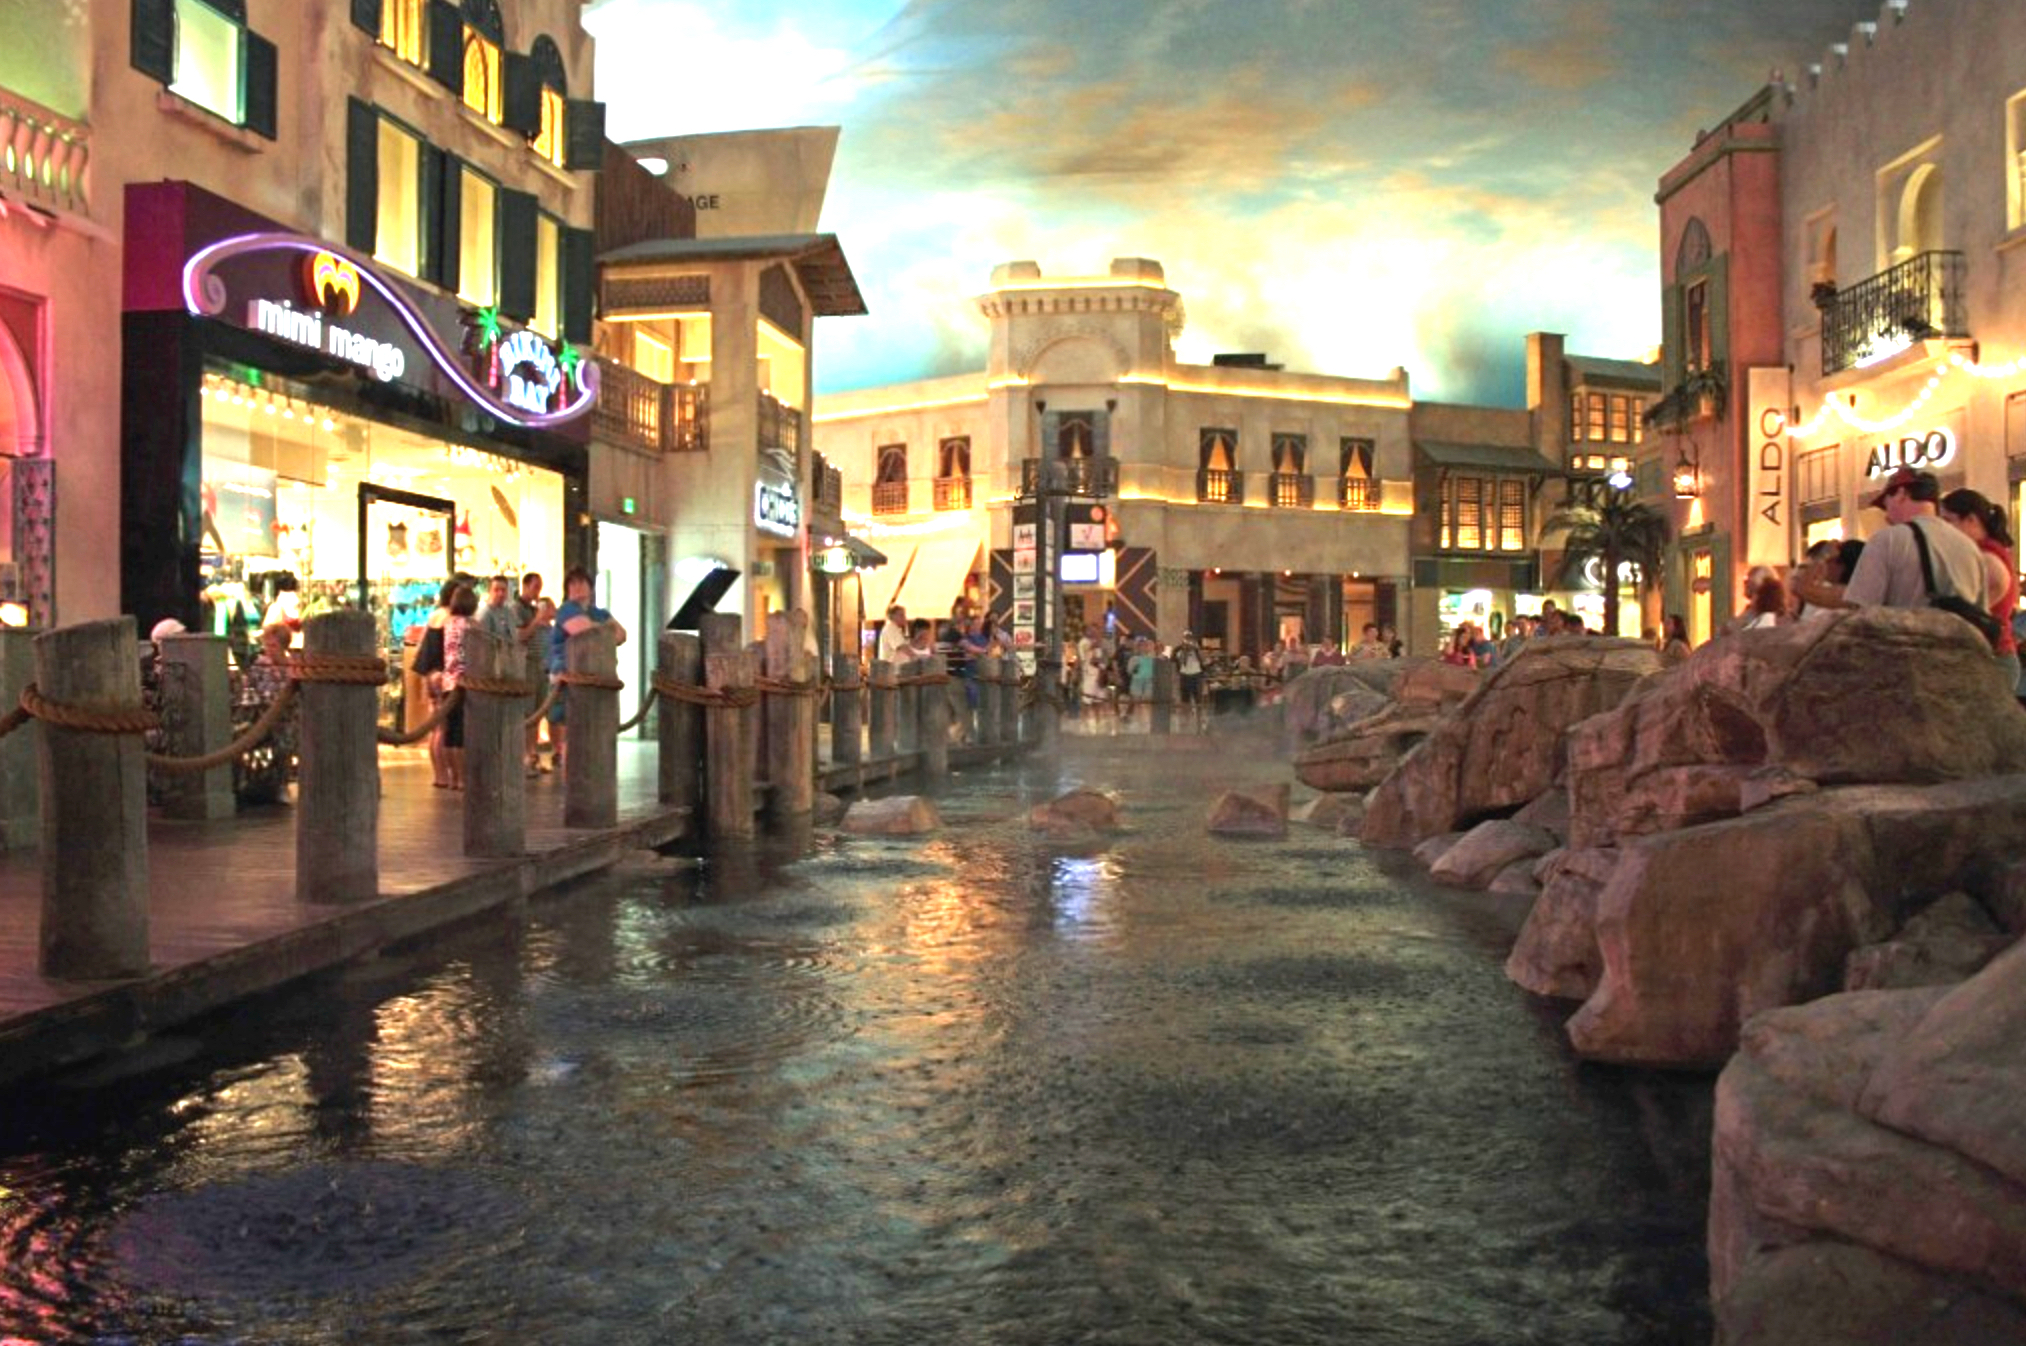
\includegraphics[height=3.25in]{Cover2.jpg} 
%%\end{figure}
%\begin{figure}[h!] %  figure placement: here, top, bottom, or page
%   \centering
%   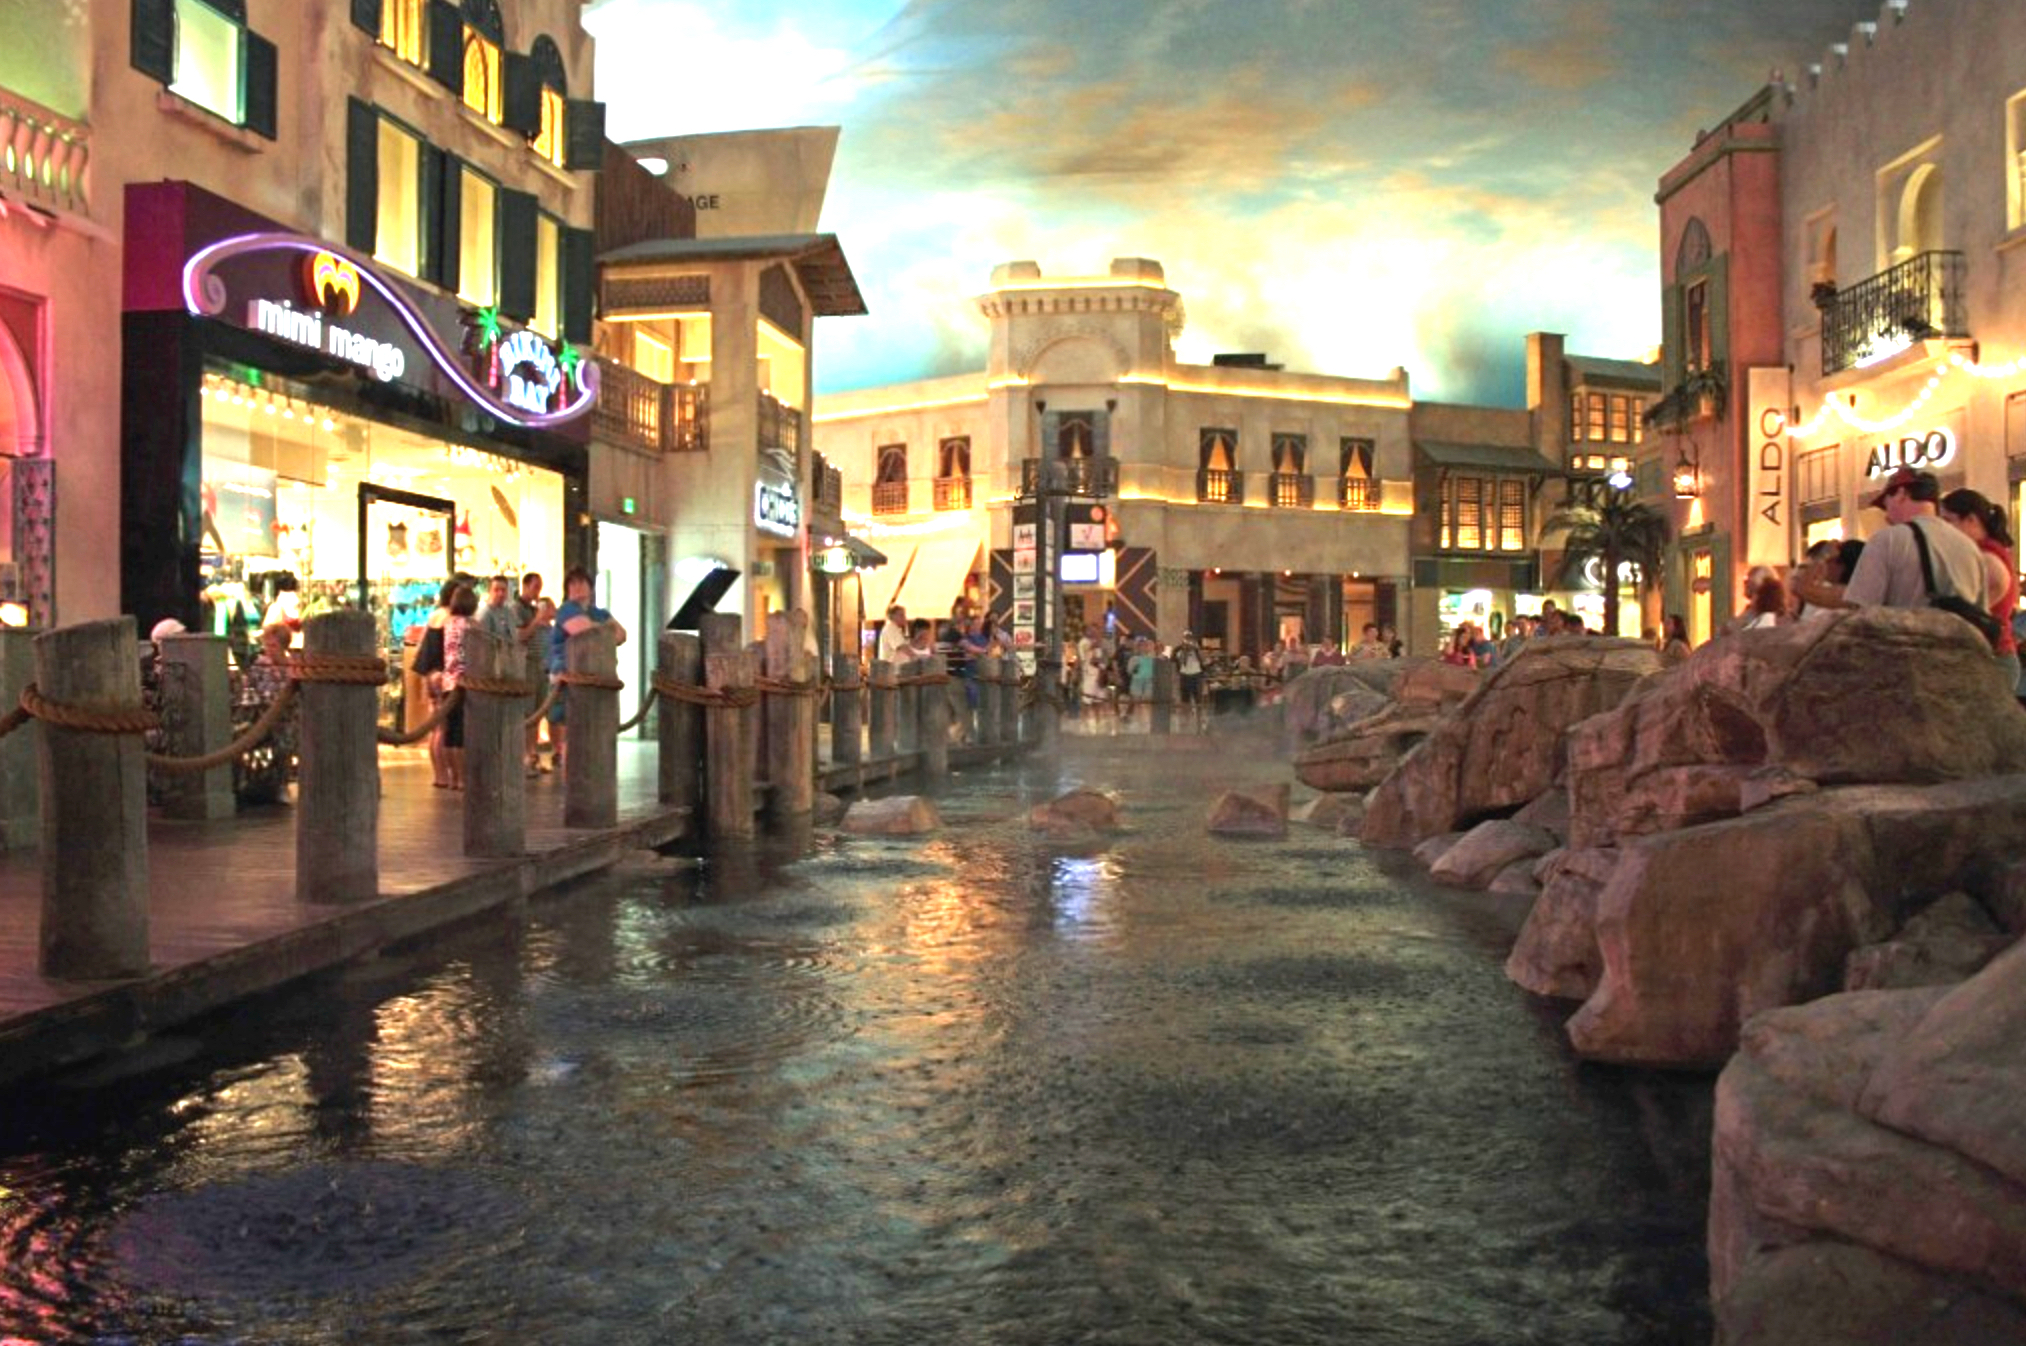
\includegraphics[width=6in]{Cover2.jpg} 
%\end{figure}
%\begin{figure}[h!] %  figure placement: here, top, bottom, or page
%   \centering
%%   \includegraphics[width=5in]{Cover.jpg} 
%\end{figure}
%
%\endgroup
%
%~\newpage

%\begingroup
%\begin{center}
%{\textbf{{ CE 3305 Engineering Fluid Mechanics} \\ Exercise Set 17 \\ Summer 2018 -- GERMANY} }
%\end{center}
%\endgroup
%\begingroup
%~\newline
%\textbf{Purpose} : Apply network hydraulics principles to compute discharges and pressures in a pipeline network. \\
%\textbf{Assessment Criteria} : Completion, results plausible, format correct, \textbf{R} script shown\\~\\
%\textbf{Exercises}:


%\tableofcontents
%%%%%%%%%%%%%%%%%%%%%%%%%%%%%%%%%%%%%%%%
%%%%%%%%%%%%%%%%%%%% CHAPTER 1 %%%%%%%%%%%%%%%%%%%%%%%%%%%%%%%%%%%%%
%%%%%%% INTRODUCTION %%%%%%%%%%%%%%%%%%%%%%%%%%%%%%%%%%%%%%%%%%%%%%%
\section{Introduction and Getting Started}
In the 1990s Civil Engineering programs reduced programming courses in a effort to recover hours for other topics -- a logical decision at the time, but with some consequences.  
The philosophy was that engineers would not need to be able to write computer programs, but instead just use them.  
Microsoft Excel and Lotus 1-2-3 were the dominant spreadsheet software programs (Borland QuatroPro was a close third), and with macro instruction capability, much legitimate engineering computation could be performed within these tools.  
In fact I developed Excel spreadsheets that could solve multi-dimensional diffusion problems (3D groundwater flow) using fully implicit finite difference methods.  These spreadsheets were slow relative to MODFLOW, but you could watch the solutions evolve -- ultimately the process was deemed a waste, because of the ever present ``... there is no longer a need for engineers to be able to write programs.''
Later on I developed spreadsheets to perform pressurized pipe network simulation, gradually varied flow simulation, and rudimentary water-hammer and St-Venant equation solutions.  The spreadsheets were never really practical (yes they worked well, produced the same results as professional products, but were always intended a pedagogical tools), but they proved an important point -- if you could teach a computer to follow an algorithm it made you a more self-help user of the professional tools.

In 2014 several of my students expressed desire to understand programming -- they all know how to write code, but feel they don't know how to build algorithms (and implement them).   This workbook is an attempt to remedy that student self-identified weakness.   I conducted several one-to-one classes (as special topics); they learned a lot, I learned even more.  This book is a tribute to their interests.

The workbook plan is to introduce a programming tool -- I have selected \textbf{R} because it has a rich development environment already available, graphics is almost trivial, then apply that tool to selected hydraulics problems of practical value.  In the end the reader ends up with a toolkit that can either stand-alone, or more likely supplement professional tools they will eventually use.

 \textbf{R} is freeware, but it is built and maintained by a consortium of programmers and statisticians.  They have evolved the environment to work on most of the main architectures (MacOS, Windows, Linux); there are even parallel processor and GPU builds available, and a company called RStudio provides the APIs to even run it server side.  Much of the underlying code is C, C++, and well proven FORTRAN routines.
%%%%%%%%%%%%%%%%%%%%%%% CHAPTER 2 %%%%%%%%%%%%%%%%%%%%%%%%%%%%%%%
%%%%%% Getting Started %%%%%%%%%%%%%%%%%%%%%%%%%%%%%%%%%%%%%%%%%%%%%%%
\subsection{About \textbf{R}}
\textbf{R} is a open source envrionment that runs on Windows, Linux/UNIX, and Mac OS X.  The individual binaries are unique to each OS and architecture, but \textbf{R} ``source'' is interchangeable among machines.  With very minor differences, an \textbf{R} script will run equally well on any machine.

\textbf{R} is a statistical analysis tool, it is also a programming tool and language, it is also a nearly ``publication'' quality graphics tool.  Naturally all this capability comes at a cost (especially since the software is distributed for ``free'') --- learning to do more than simple calculations takes some time (not much), but the skill is highly perishable.  You will need to keep notes, or copies of your \textbf{R} scripts for future reference.  Relearning after some time away from \textbf{R} is pretty simple, so the modeler only has to pay the steep learning cost once.

The remainder of this essay shows how to obtain and install \textbf{R} on a Windows machine.  Macintosh and Linux installs are accomplished in a similar fashion.  For the truly insane, the entire envrionment can be built from source on any machine with PERL, gcc, and gfortran compliers (default in Linux, easy to obtain for other architectures).

\subsection{Getting Started}
The first step required (for using \textbf{R} as a programming tool) is to install \textbf{R} on your computer.
The source of the binary builds is the same regardless of the underlying operating system -- the Comprehensive R Archive Network (CRAN for short).
The remainder of this chapter shows how to get the tool running on the three main operating systems in current practice.
\subsubsection{Windows Users}
The purpose of this section is to demonstrate how to get \textbf{R} running on a Windows computer.  This document assumes the following:
\begin{enumerate}
\item You have internet connection.
\item You have sufficient user privileges to install software on your machine.  (If you need someone else to install, I did my install by running the installer as a local administrator --- obviously you need the password)
\item You have 60MB or so of vacant disk space on the system directory.
\end{enumerate}

The step-by-step guide is presented as a series of screen captures.  Obviously adjust inputs to fit your machine.  The version in these screen captures is quite dated --- use the most recent, stable version offered on CRAN (Comprehensive R Archive Network).\footnote{I have updated the screen captures for Windows 10 --- so these should replicate the steps.}

%\section*{}

\begin{figure}[h!] %  figure placement: here, top, bottom, or page
   \centering
   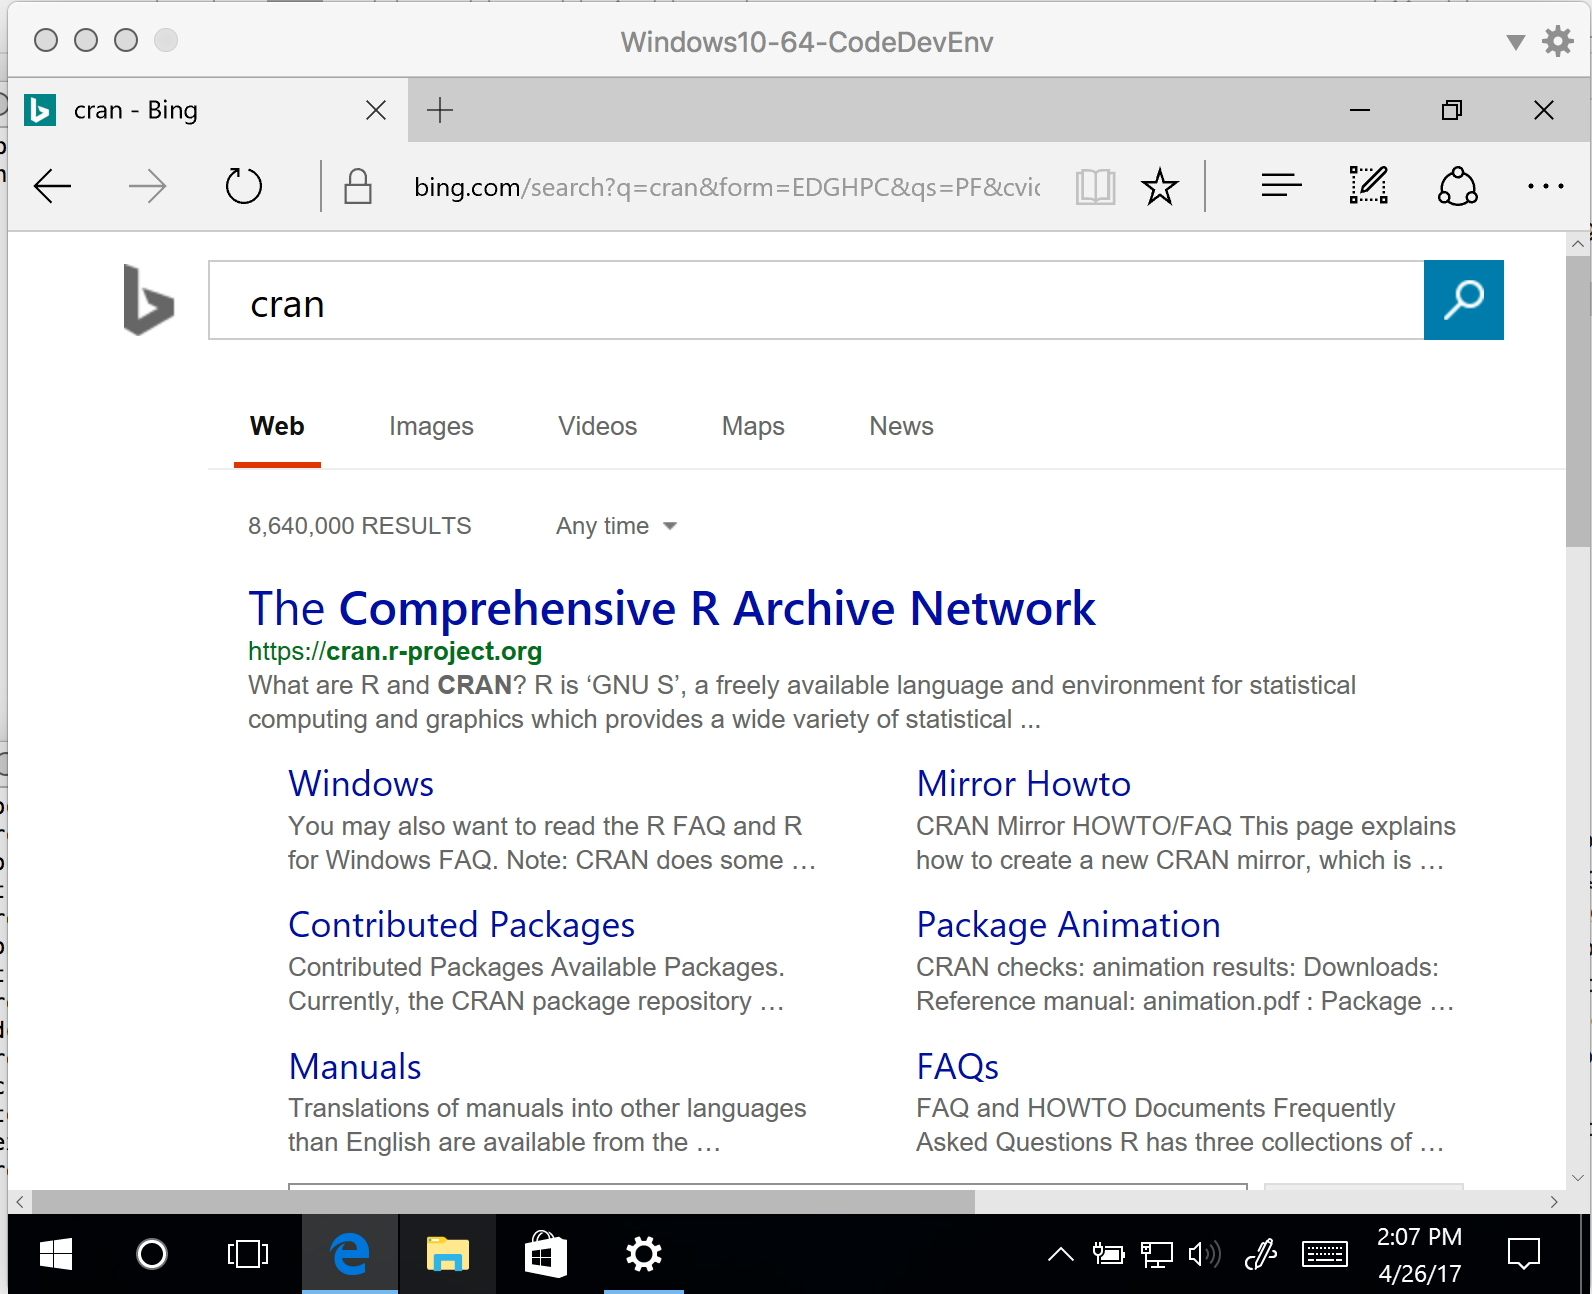
\includegraphics[width=4.5in]{./1-Introduction/googleR.jpg} 
   \caption{Google ``R'' (alternatively google CRAN)}
%   \label{fig:example}
\end{figure}

\begin{figure}[h!] %  figure placement: here, top, bottom, or page
   \centering
   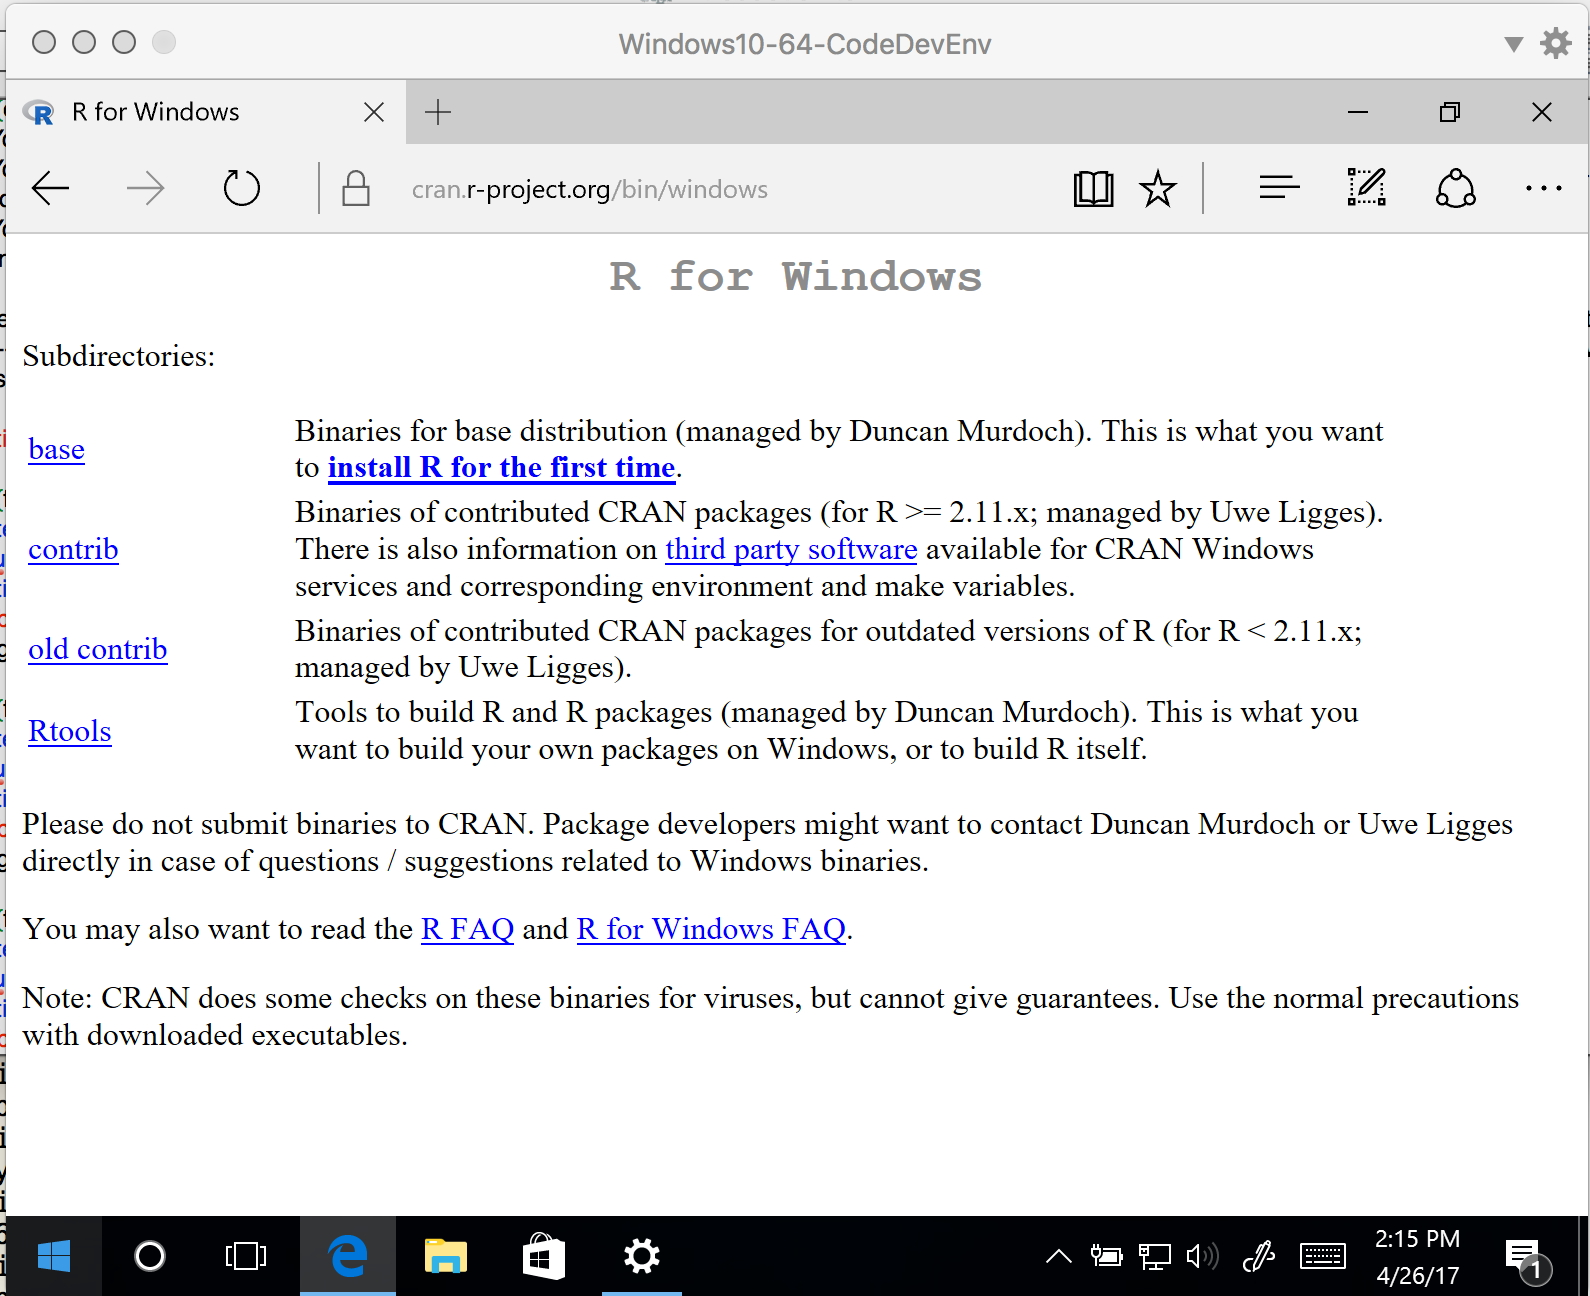
\includegraphics[width=4.5in]{./1-Introduction/gnuRproject.jpg} 
   \caption{Taking the ``Windows Link''}
%   \label{fig:example}
\end{figure}

\begin{figure}[h!] %  figure placement: here, top, bottom, or page
   \centering
   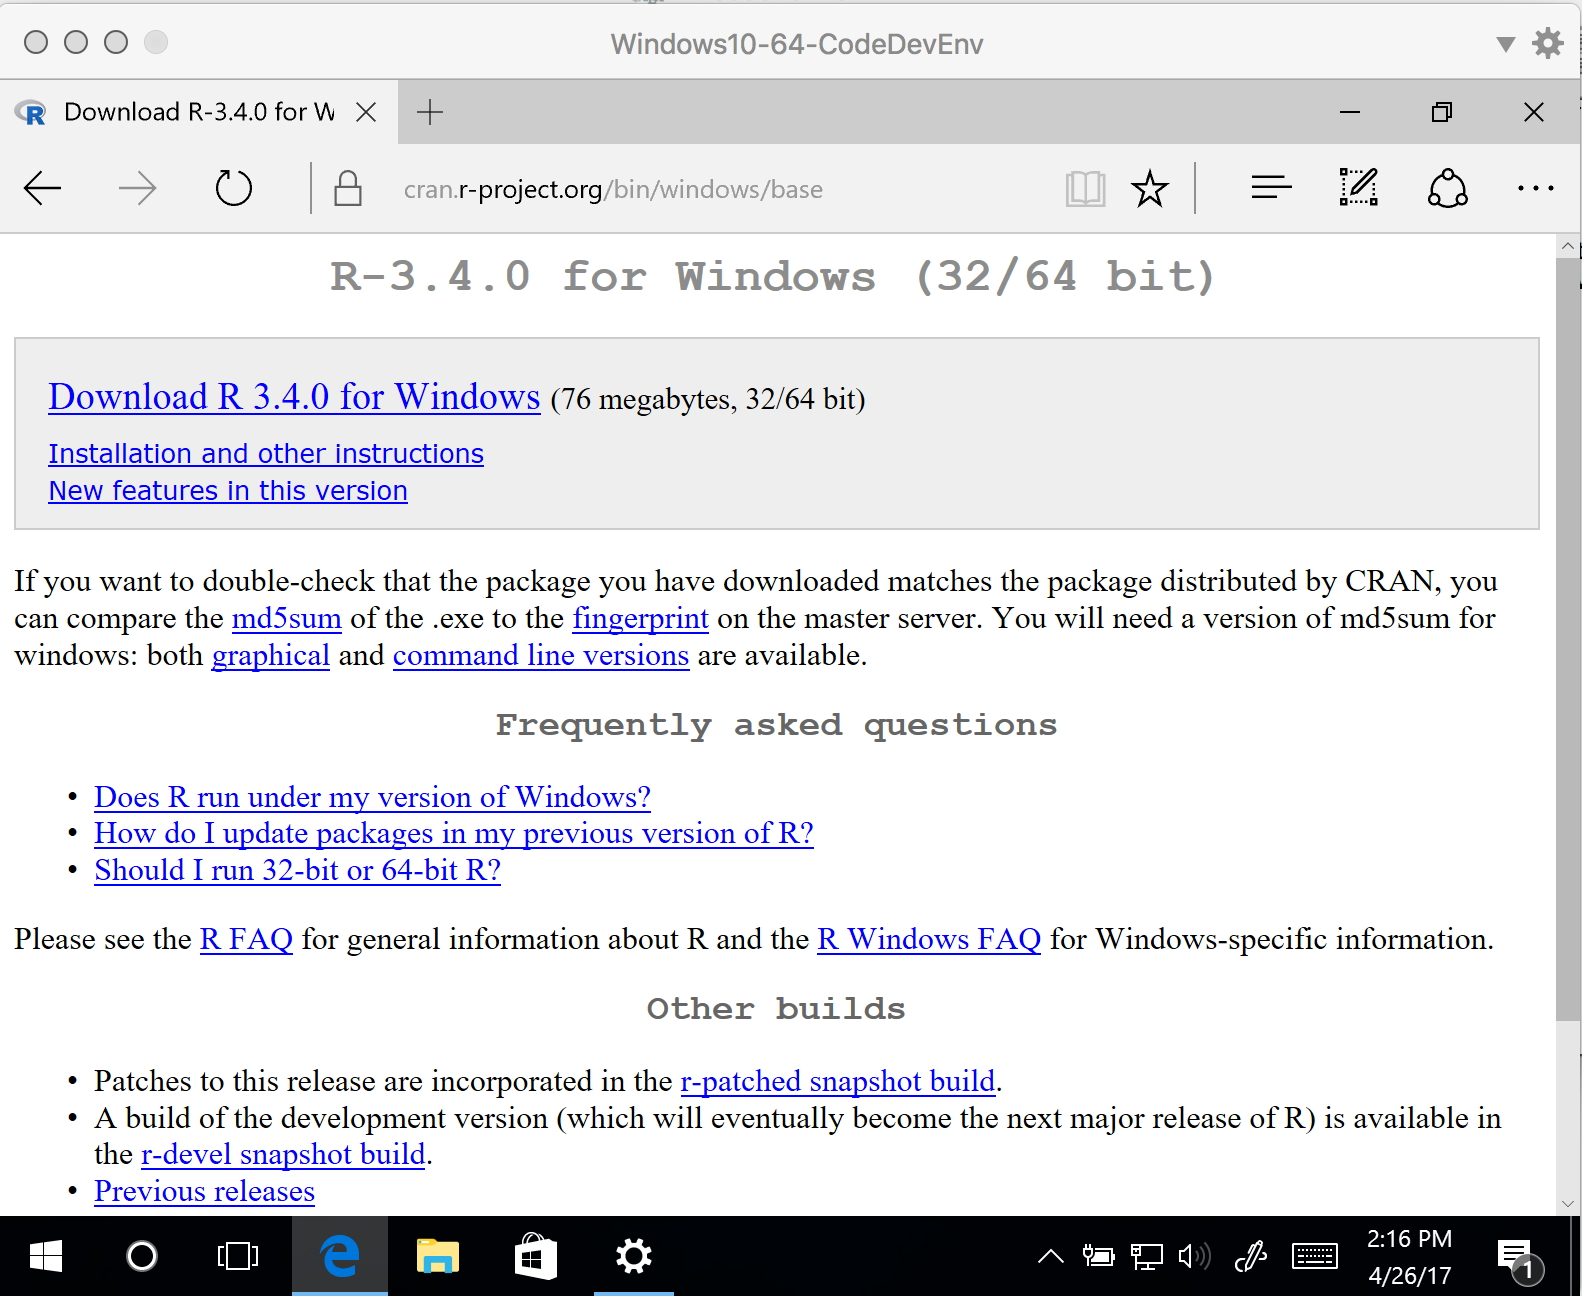
\includegraphics[width=4.5in]{./1-Introduction/downloadR.jpg} 
   \caption{Choose ``Install R for the First Time" -- goes to the download page.  We will next select ``Download R \dots'' and it should download a windows installer.  Choose ``save'' when prompted.}
%   \label{fig:example}
\end{figure}

\begin{figure}[h!] %  figure placement: here, top, bottom, or page
   \centering
   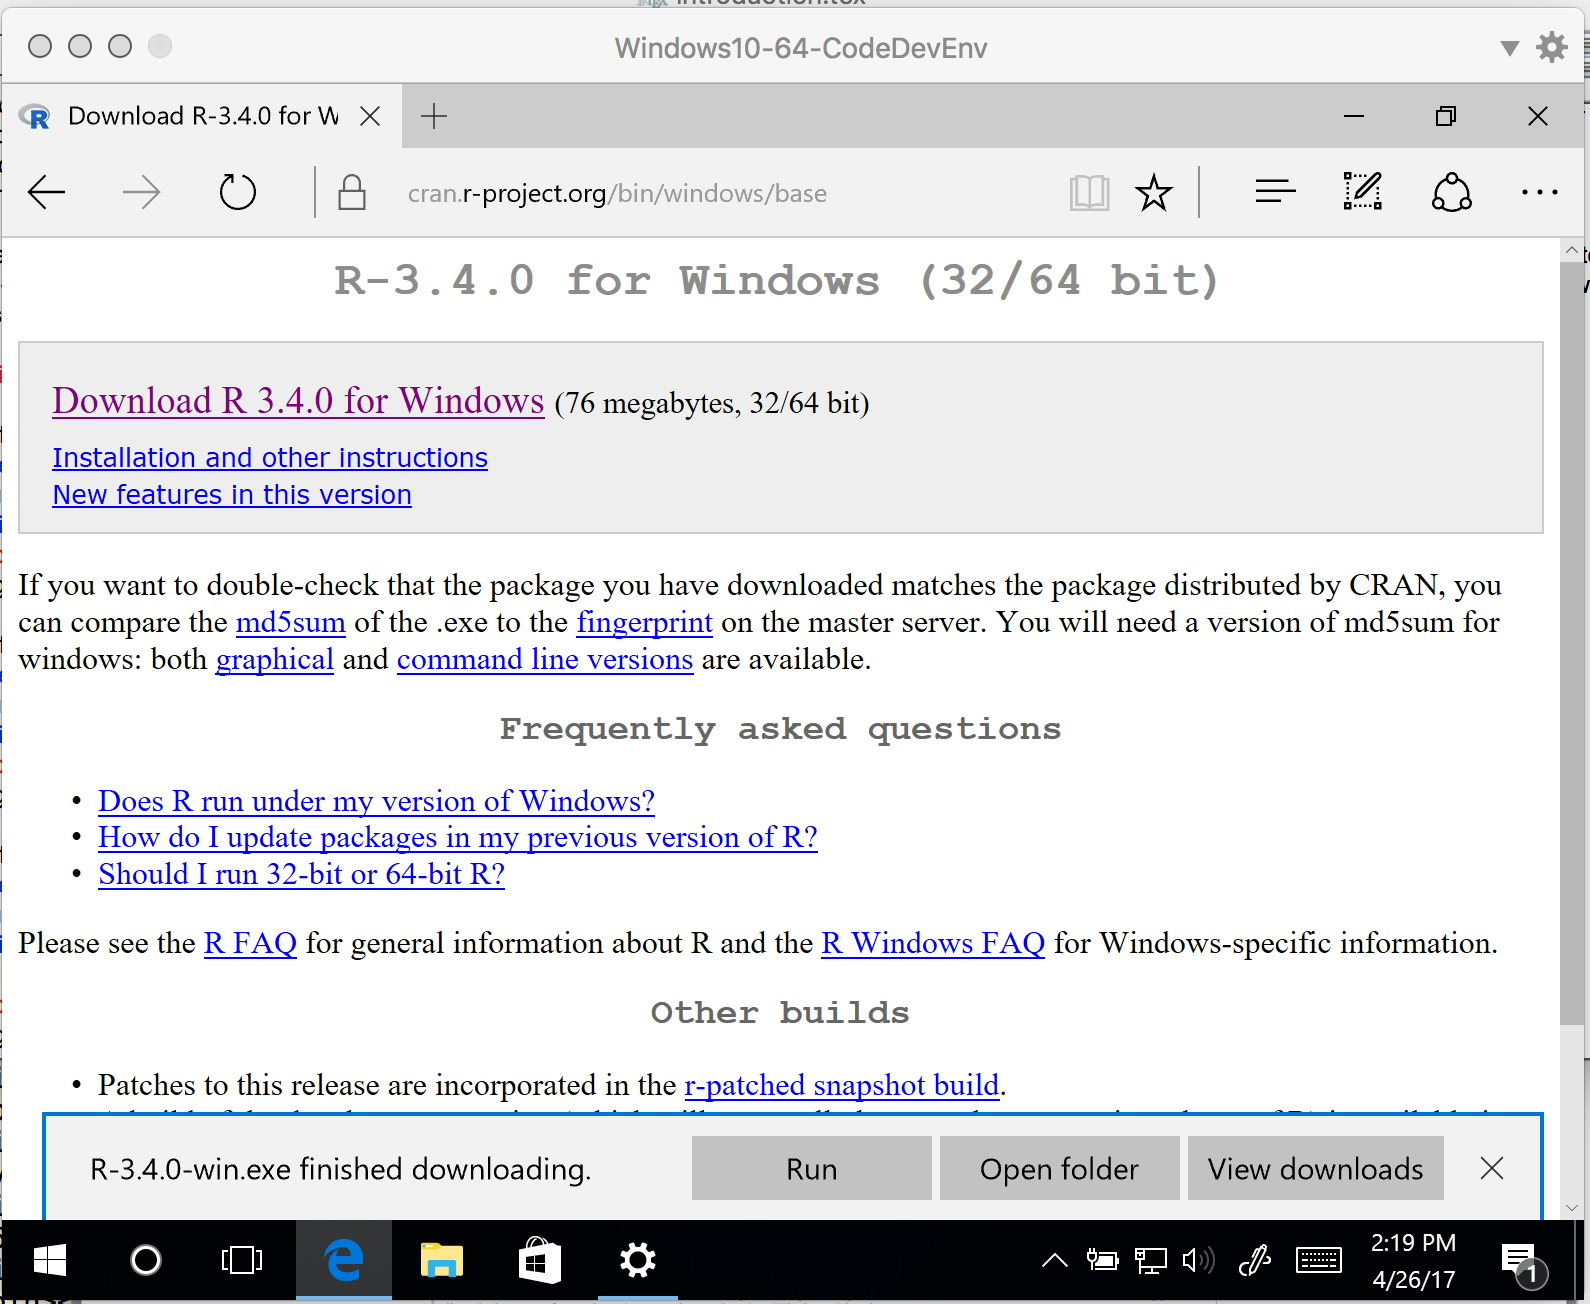
\includegraphics[width=4.5in]{./1-Introduction/repositoryR.jpg} 
   \caption{Download arrived.  Now run the installer (you need install privileges -- if its your personal laptop, then your regular user account should work). }
%   \label{fig:example}
\end{figure}

\begin{figure}[h!] %  figure placement: here, top, bottom, or page
   \centering
   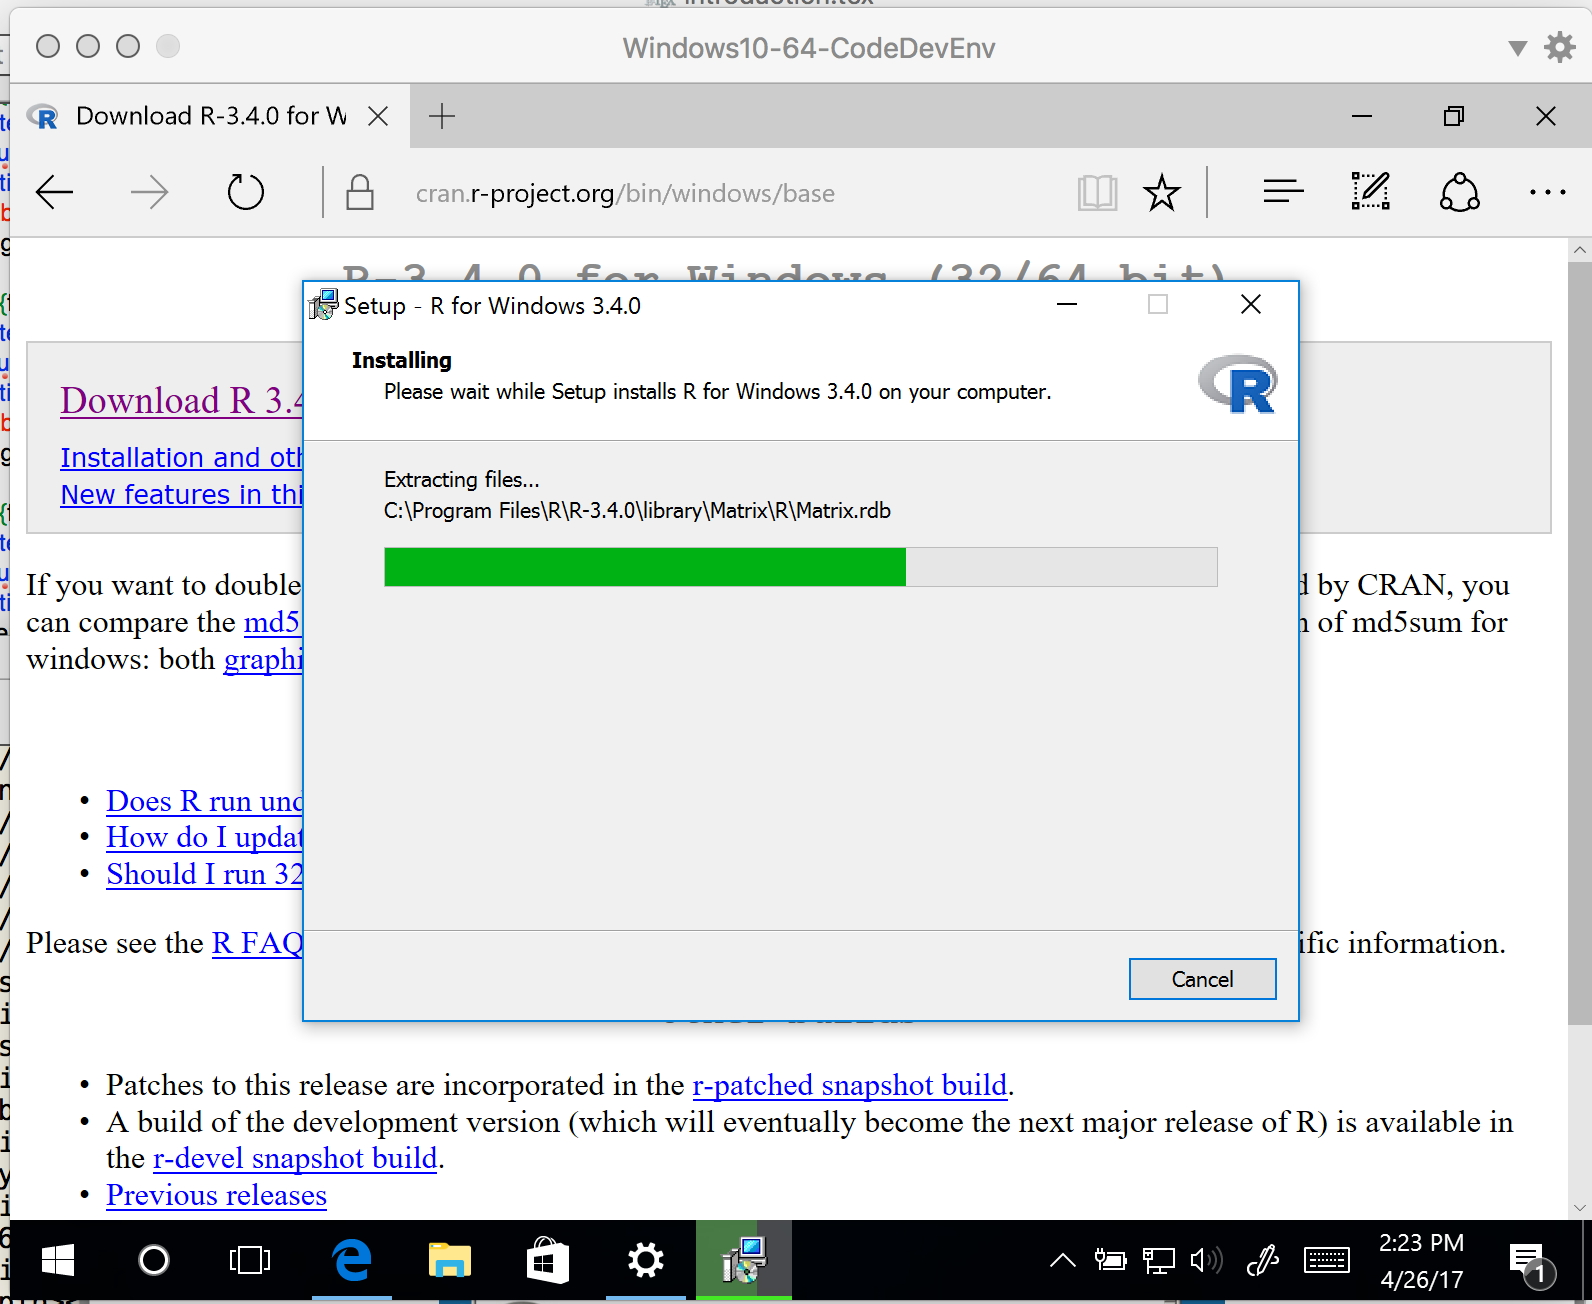
\includegraphics[width=4.5in]{./1-Introduction/chooseOS.jpg} 
   \caption{Installer run in progress.  Accept the defaults -- its just easier and works.   Later you can re-install elsewhere in your filesystem.}
%   \label{fig:example}
\end{figure}

\begin{figure}[h!] %  figure placement: here, top, bottom, or page
   \centering
   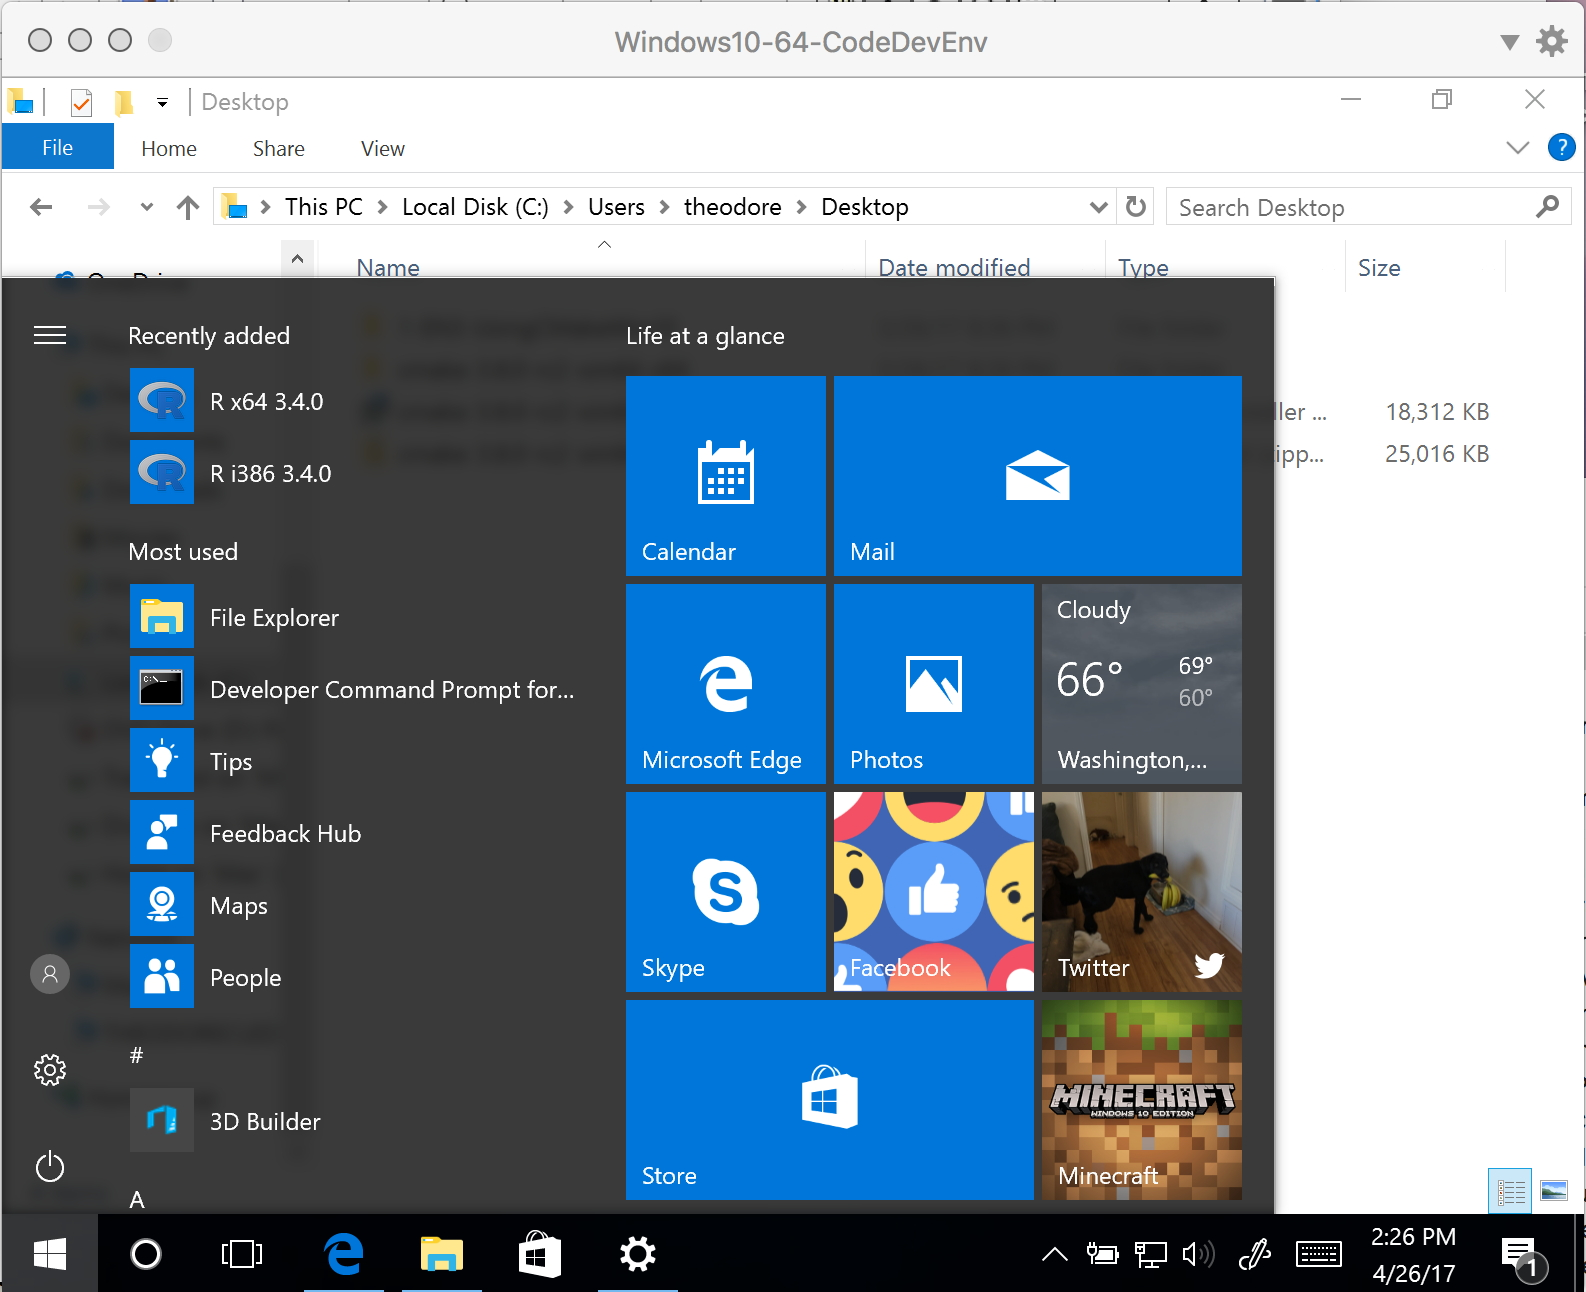
\includegraphics[width=4.5in]{./1-Introduction/baseR.jpg} 
   \caption{Installed ``R base'' packages.  Notice it installs 32-bit and 64-bit versions.  The next step is to verify the install by trying to run the program.}
%   \label{fig:example}
\end{figure}

\begin{figure}[h!] %  figure placement: here, top, bottom, or page
   \centering
   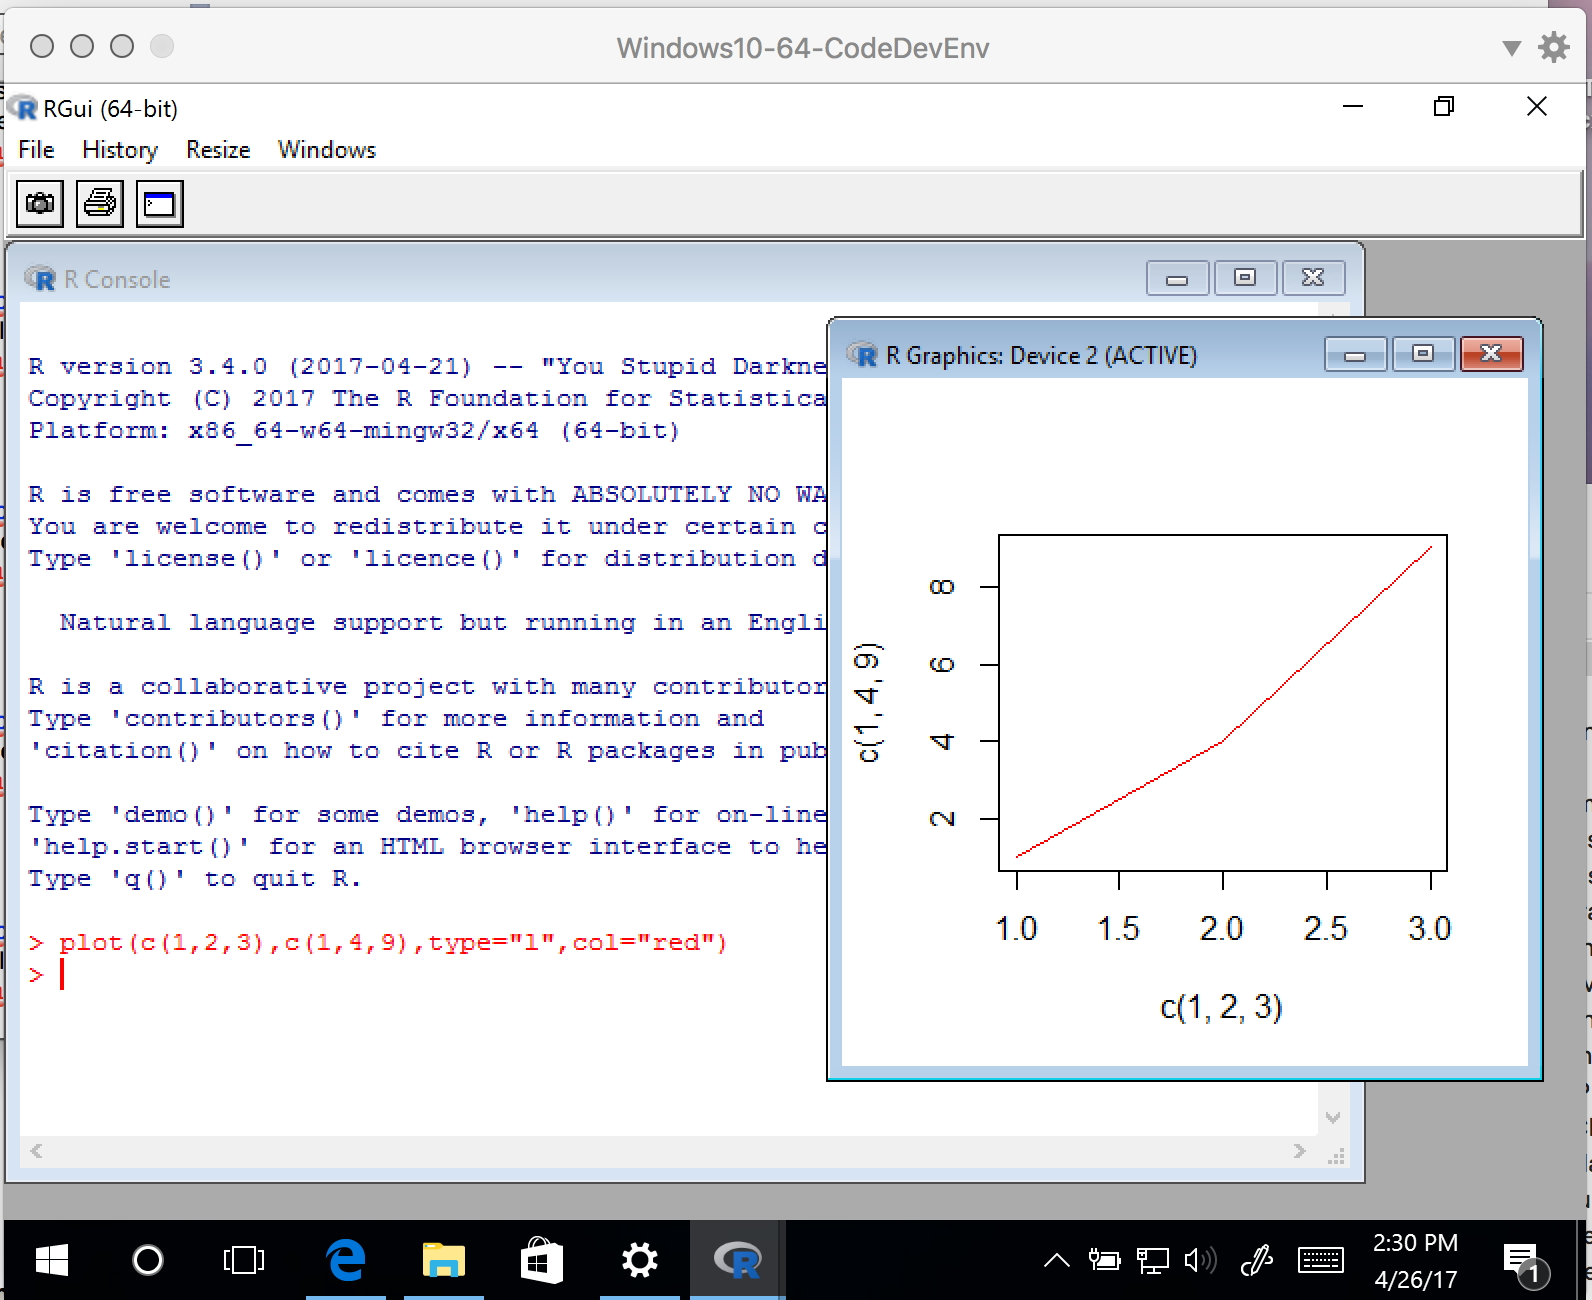
\includegraphics[width=4.5in]{./1-Introduction/installerR.jpg} 
   \caption{Run the program.  Type \texttt{plot(c(1,2,3),c(1,4,9),type="l",col="red")} into the console window.  A plot should be generated as shown.  If this works, then your install is good and now we install \textbf{R Studio}}
%   \label{fig:example}
\end{figure}

\begin{figure}[h!] %  figure placement: here, top, bottom, or page
   \centering
   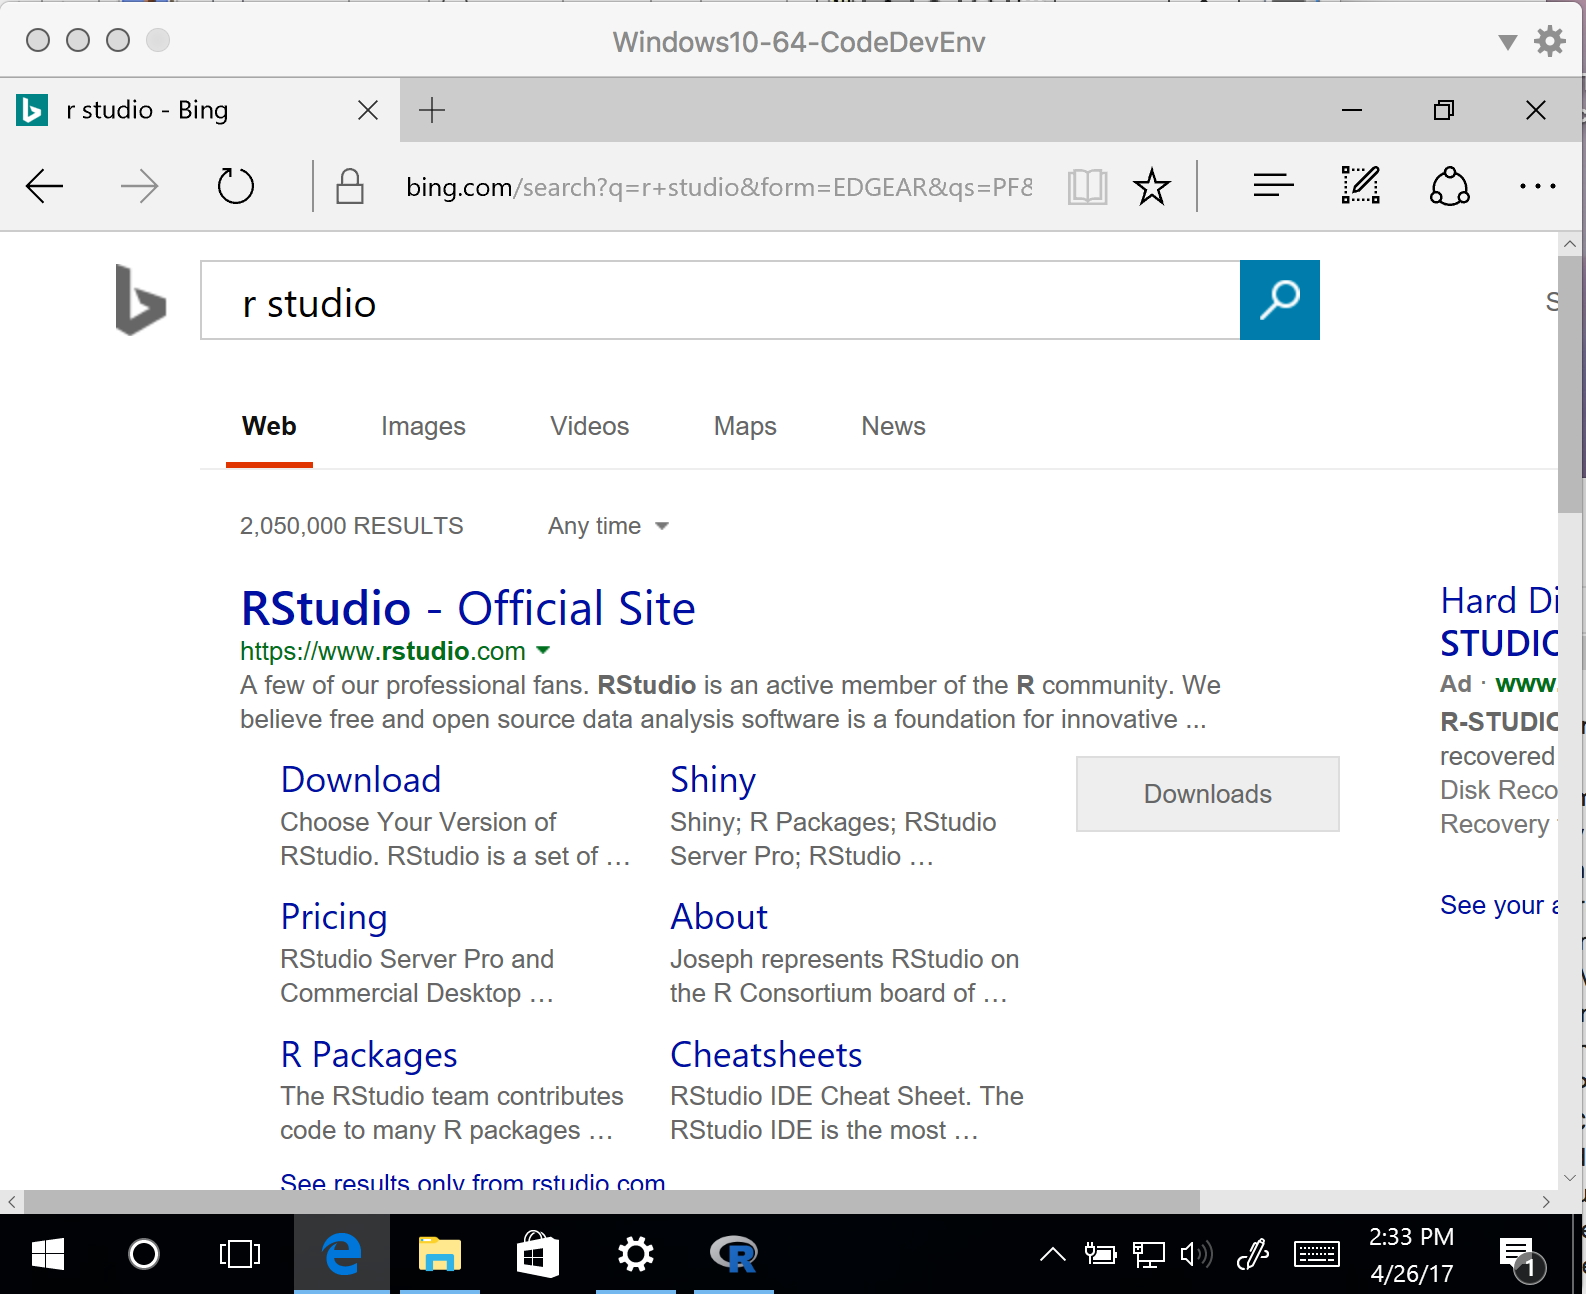
\includegraphics[width=4.5in]{./1-Introduction/downloading.jpg} 
   \caption{Search for \textbf{R Studio}.  Choose the Download link.}
%   \label{fig:example}
\end{figure}

\begin{figure}[h!] %  figure placement: here, top, bottom, or page
   \centering
   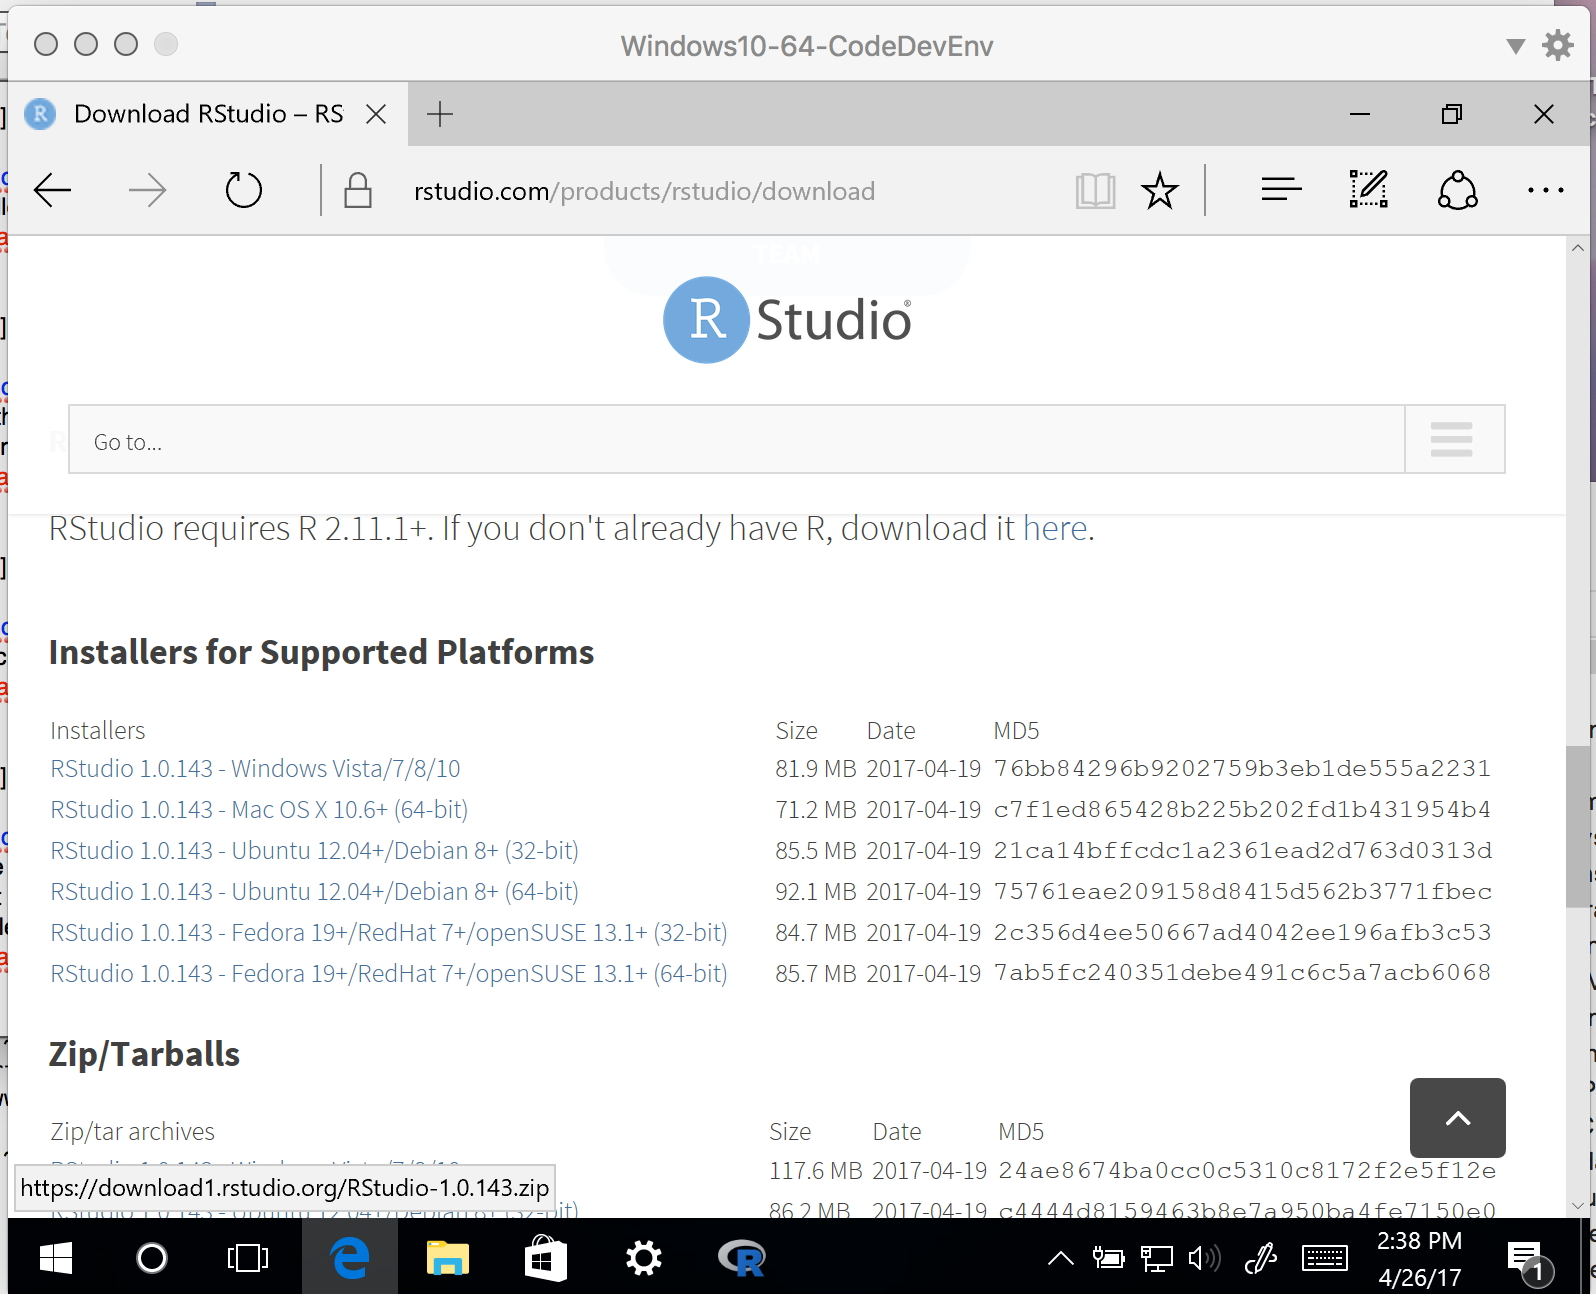
\includegraphics[width=4.5in]{./1-Introduction/runInstall.jpg} 
   \caption{In the download link scroll down to the repository.  You want to install the FREE Desktop version.  If on a windows machine, it is the top most of the installers.  Don't accidentally download the Zip/Tarballs -- all that is source code and without the compilers you cannot make much use of it.  Building from source is a challenge.  Choose the windows installer and download, select ``save'' when prompted}
%   \label{fig:example}
\end{figure}

\begin{figure}[h!] %  figure placement: here, top, bottom, or page
   \centering
   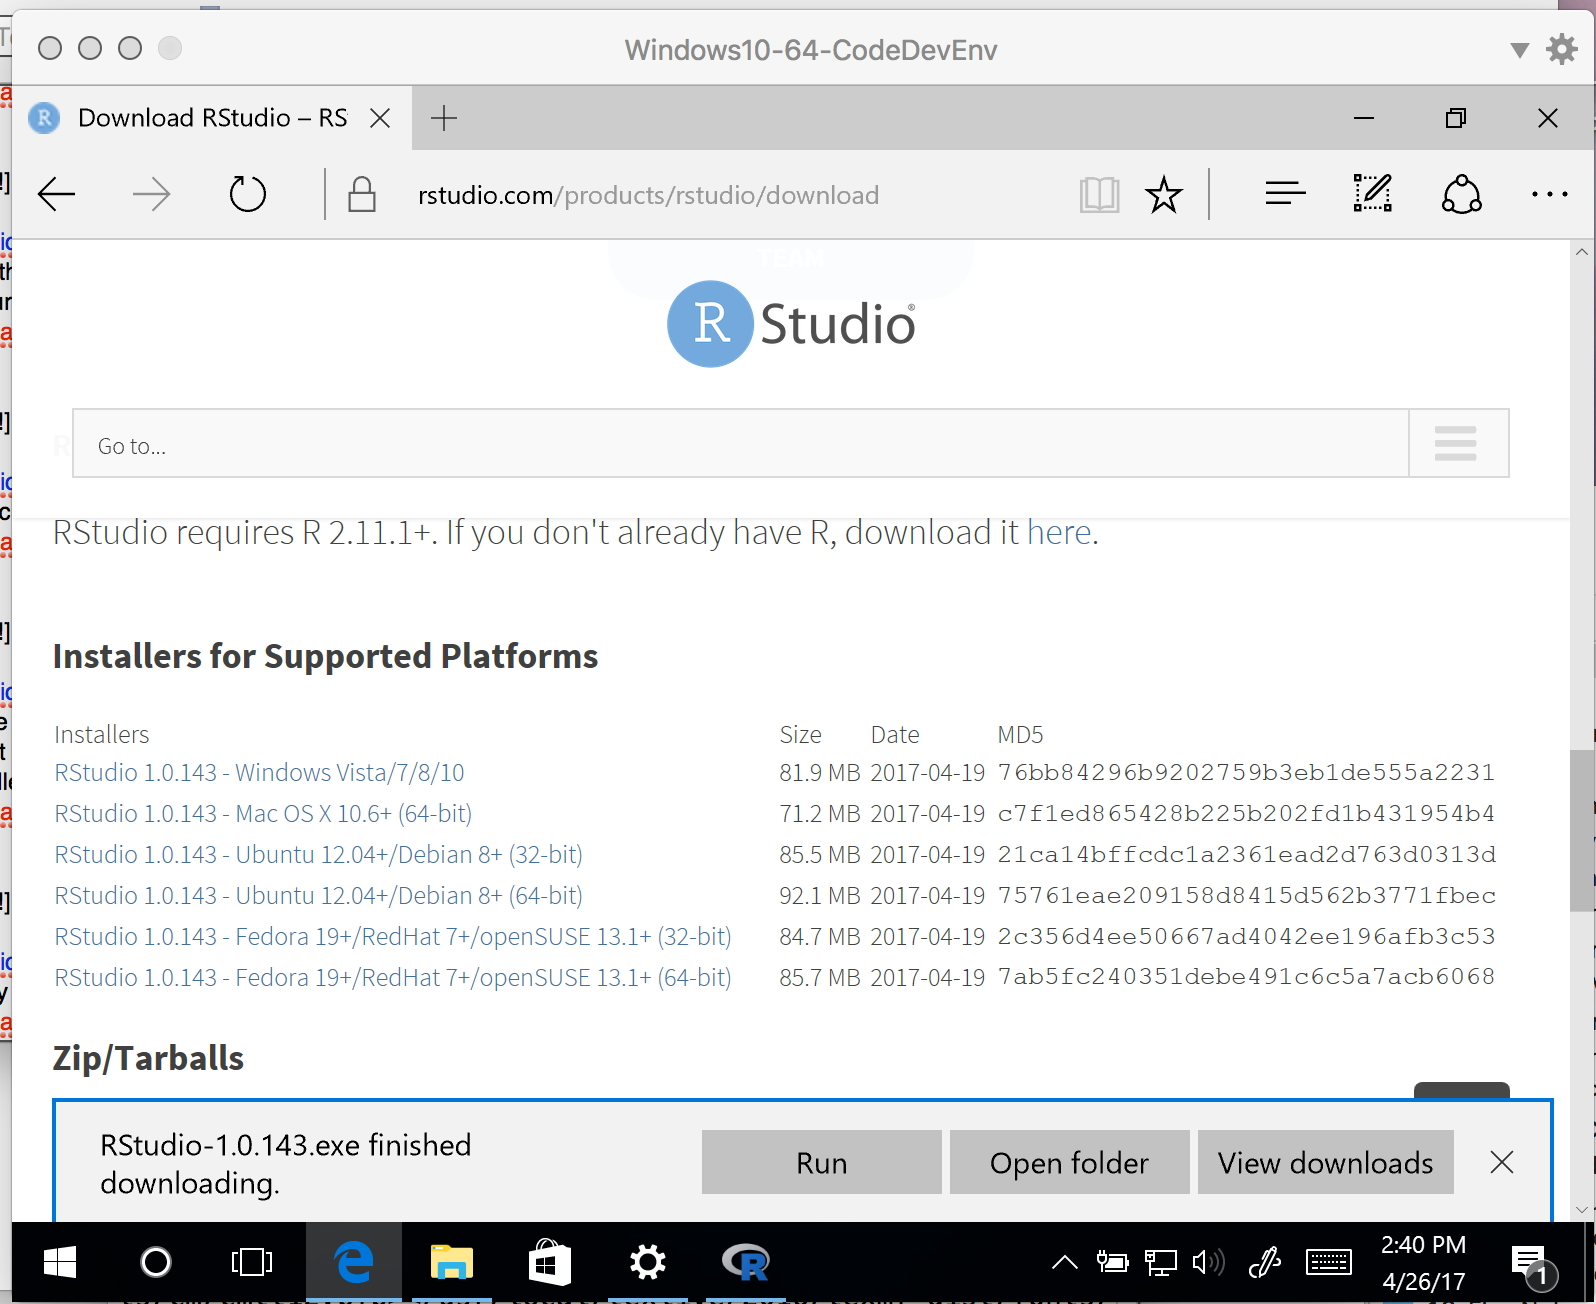
\includegraphics[width=4.5in]{./1-Introduction/repositoryR2.jpg} 
   \caption{Download arrived, run the executable (it should be a \texttt{.exe} file).  Accept the defaults during the install}
%   \label{fig:example}
\end{figure}

\begin{figure}[h!] %  figure placement: here, top, bottom, or page
   \centering
   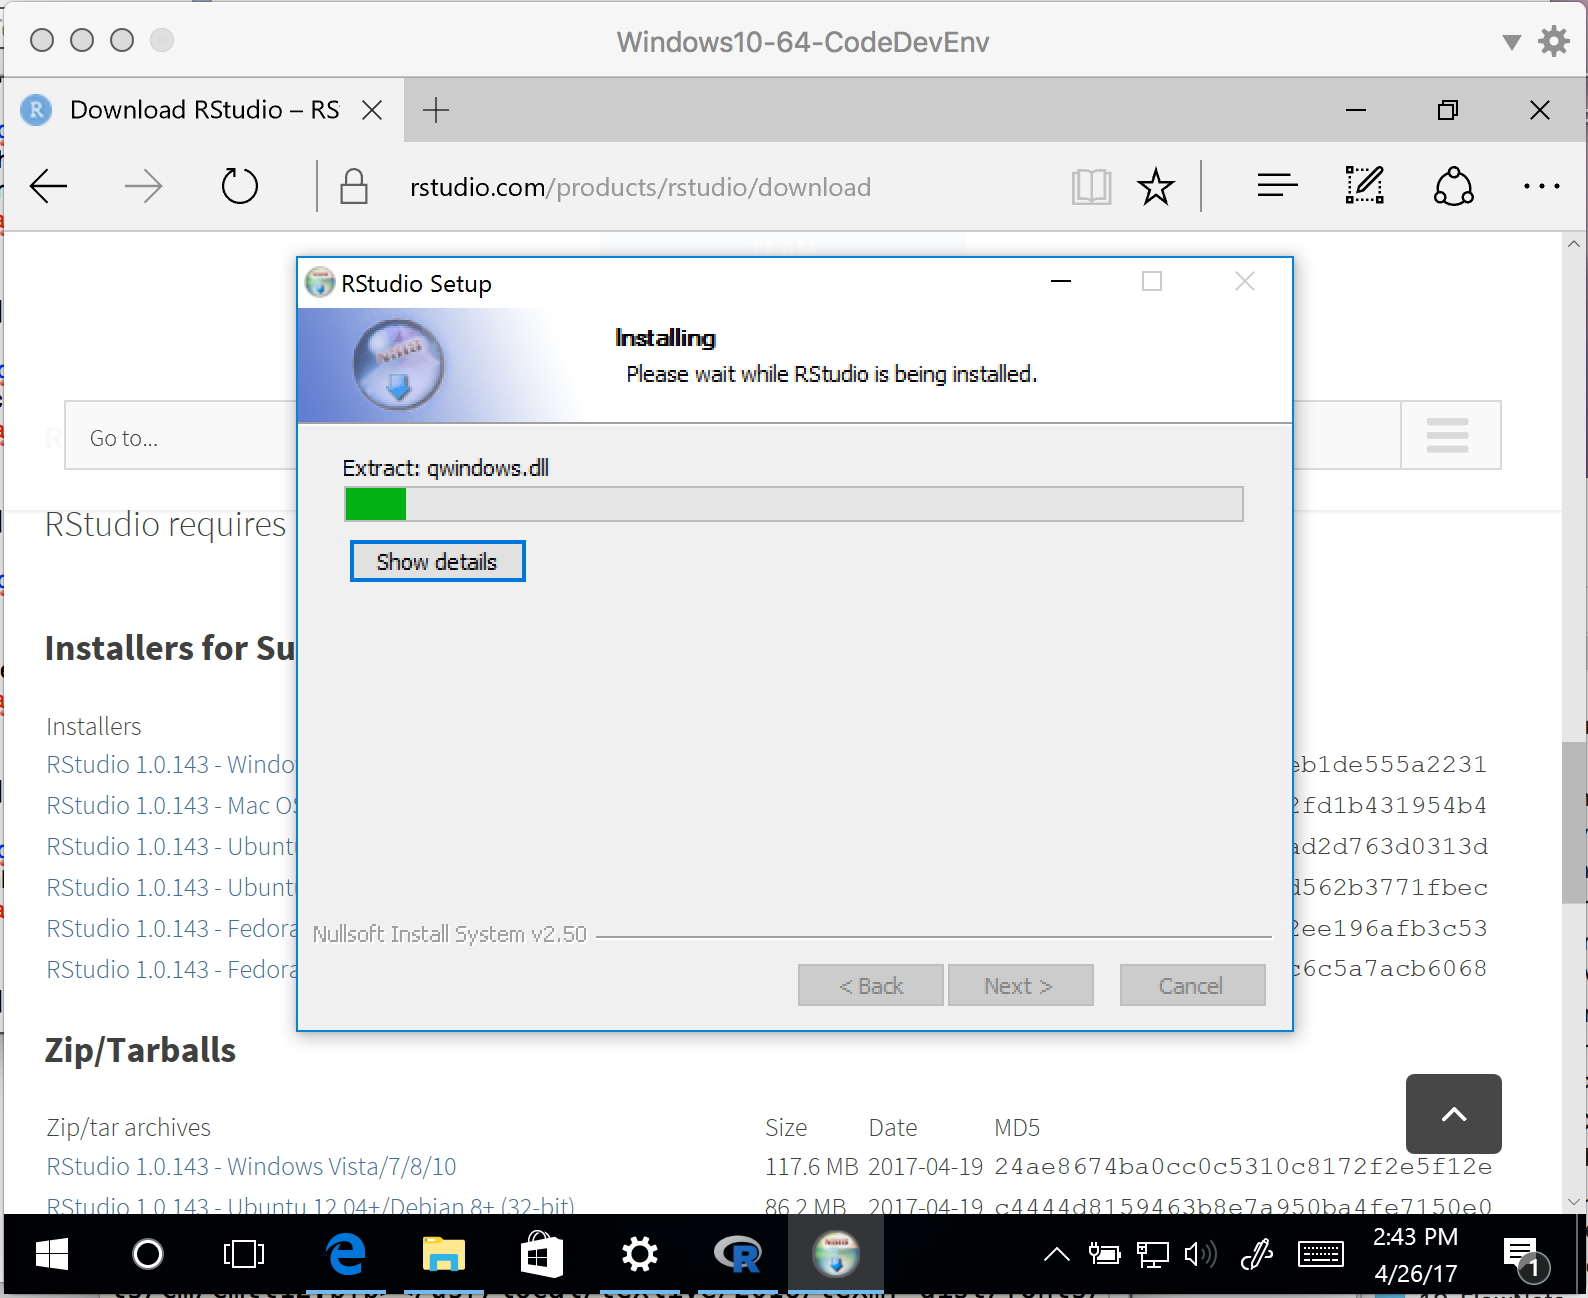
\includegraphics[width=4.5in]{./1-Introduction/runInstall2.jpg} 
   \caption{Installer in-progress.  When it completes, you should now have \textbf{R Studio} and \textbf{R} installed.  We will test the \textbf{R Studio} install using the same simple plot call}
%   \label{fig:example}
\end{figure}


\begin{figure}[h!] %  figure placement: here, top, bottom, or page
   \centering
   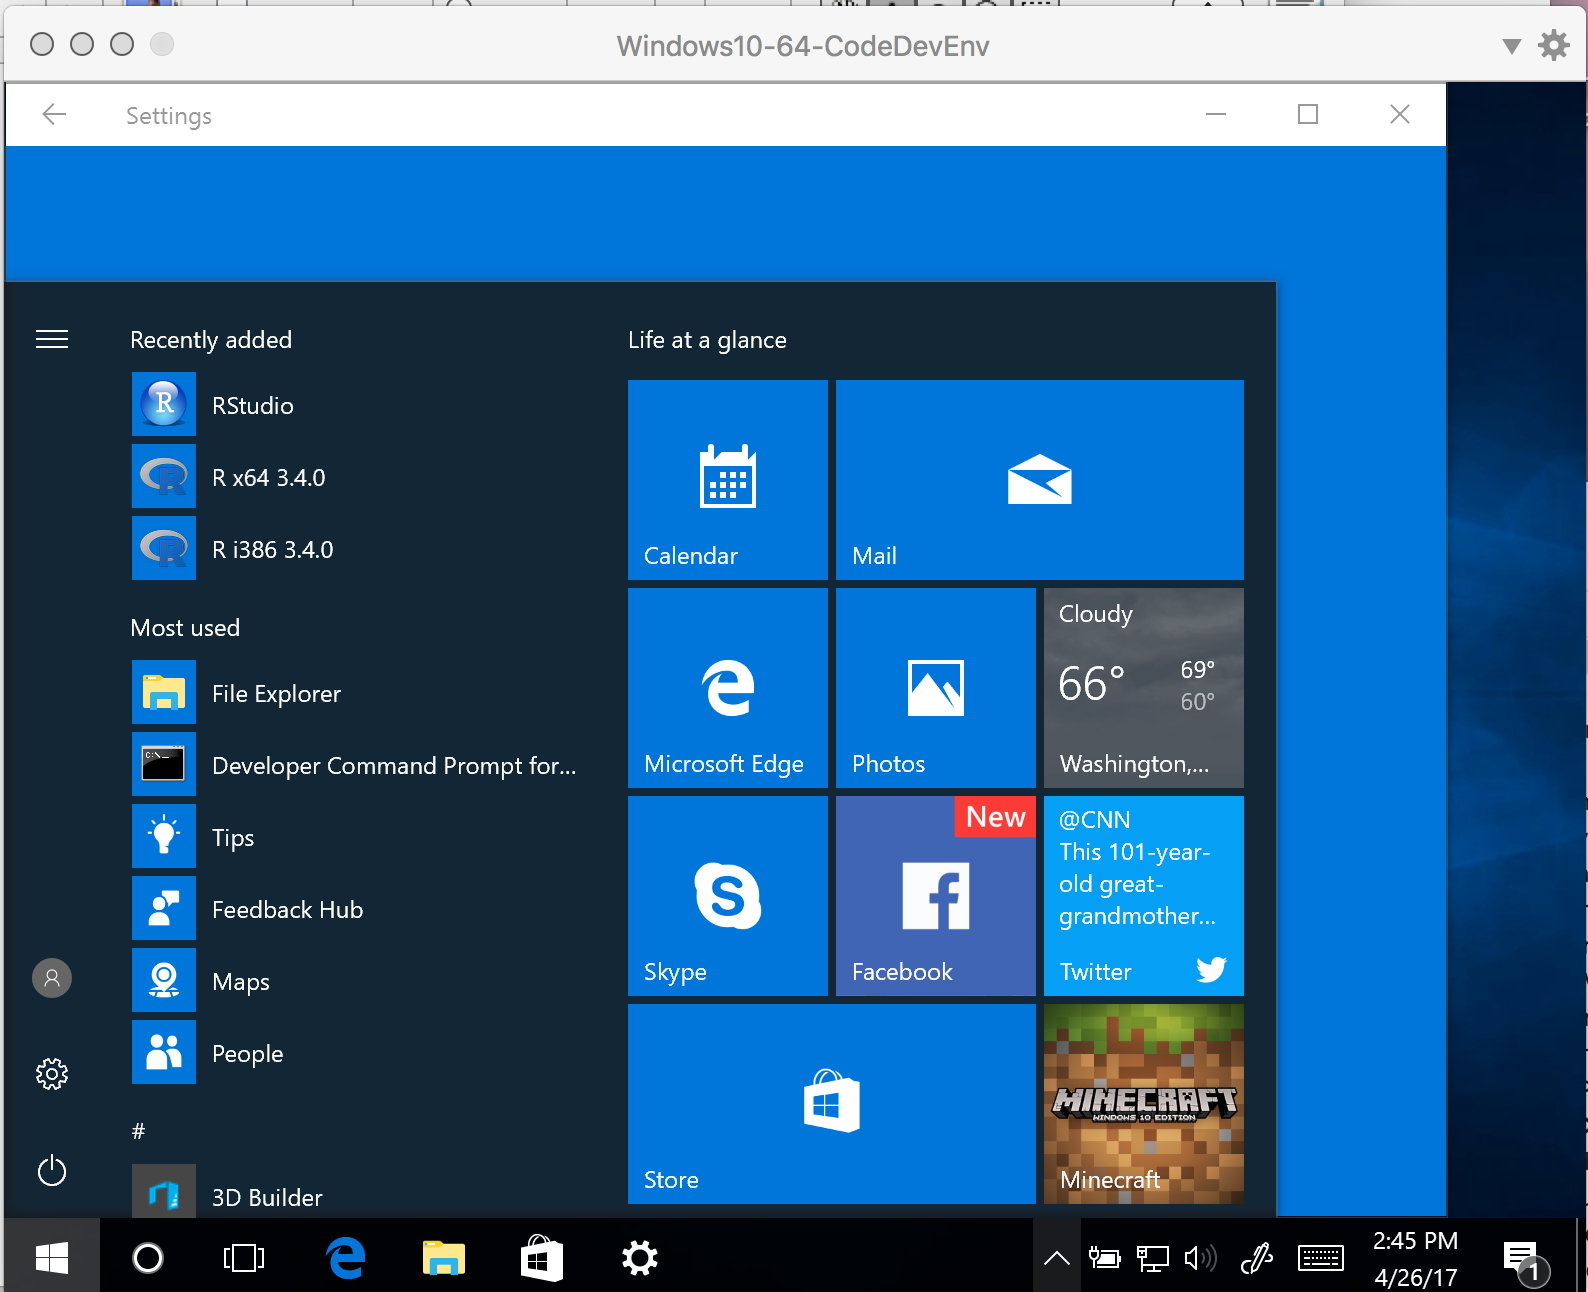
\includegraphics[width=4.5in]{./1-Introduction/verifyInstall.jpg} 
   \caption{Here we see the program is installed, now run \textbf{R Studio} to verify the install}
%   \label{fig:example}
\end{figure}

\begin{figure}[h!] %  figure placement: here, top, bottom, or page
   \centering
   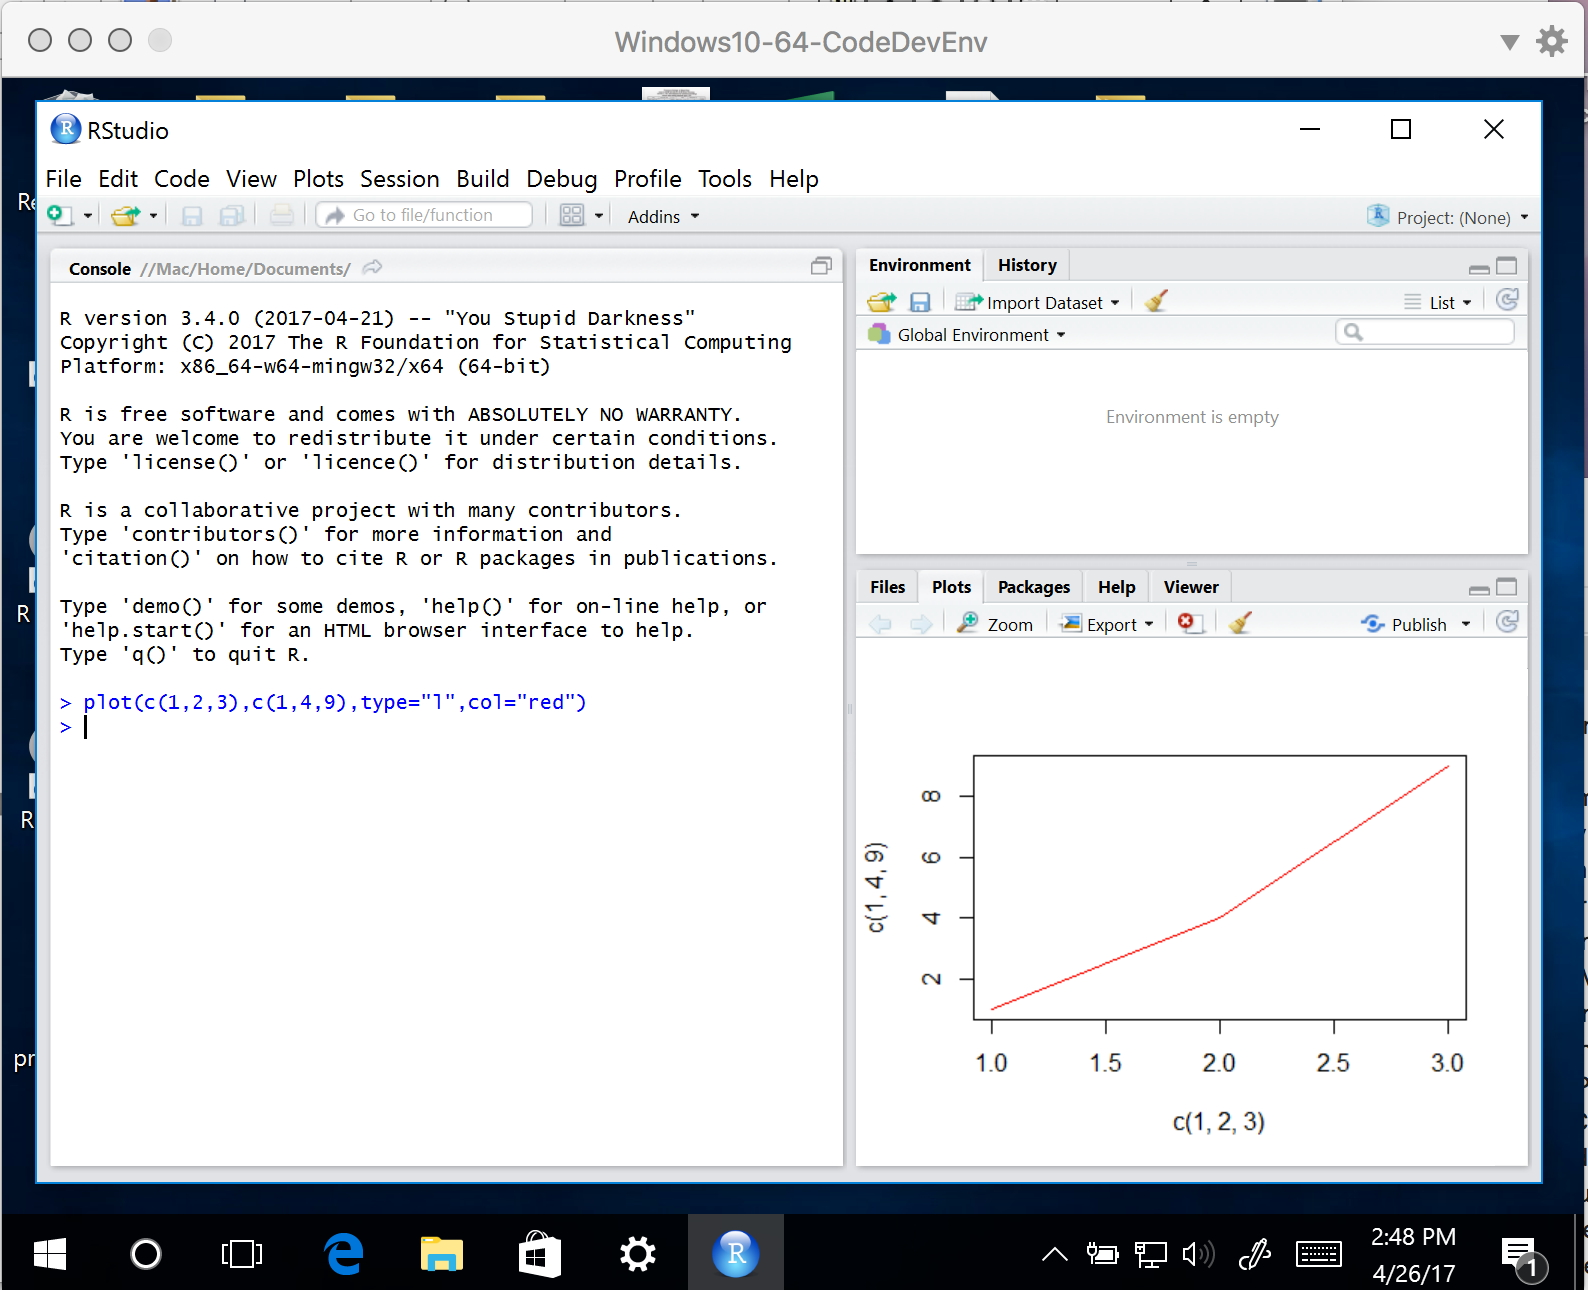
\includegraphics[width=4.5in]{./1-Introduction/verifyInstall2.jpg} 
   \caption{Type \texttt{plot(c(1,2,3),c(1,4,9),type="l",col="red")} into the console window.  A plot should be generated as shown}
%   \label{fig:example}
\end{figure}

\newpage~
\newpage~
\newpage~
\newpage~
\newpage~
\newpage~
\newpage~
Yipee!  It is running.  You can install additional packages now or later.  You should now have sufficient computation capability for the course.  
\clearpage

\subsubsection{Macintosh OSX Users}
[Replicate Windows using MacOS screen captures]
The purpose of this section is to demonstrate how to get \textbf{R} running on a Macintosh computer.\footnote{I assume no-one will be using a PPC-Based Mac.  If so, the CRAN does have PPC builds of R, but R Studio is not available; you would have to build from the source code.}  
This document assumes the following:
\begin{enumerate}
\item You have internet connection.
\item You have sufficient user privileges to install software on your machine.  (If it is your personal machine, the install may request your password, but should install.)
\item You have 60MB or so of vacant disk space on the system directory.
\end{enumerate}

The step-by-step guide is presented as a series of screen captures.  Obviously adjust inputs to fit your machine.  The version in these screen captures is quite dated --- use the most recent, stable version offered on CRAN (Comprehensive R Archive Network).\footnote{I have updated the screen captures for Windows 10 --- so these should replicate the steps.}

\begin{figure}[h!] %  figure placement: here, top, bottom, or page
   \centering
   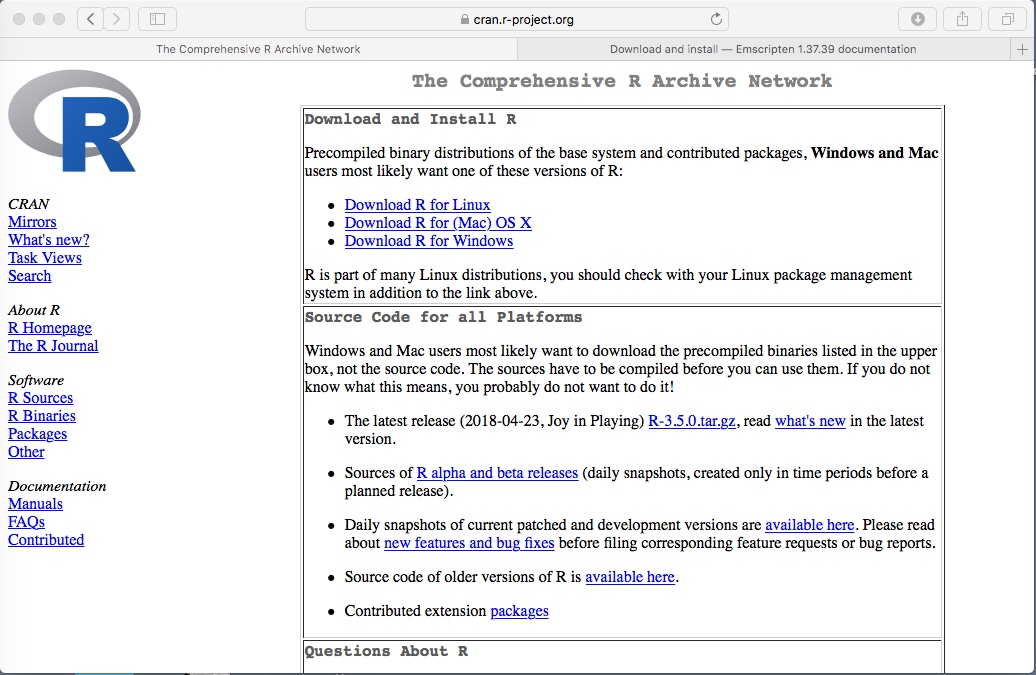
\includegraphics[width=5in]{./1-Introduction/GoogleRonMac.jpeg} 
   \caption{Google ``R'' (alternatively google CRAN)}
%   \label{fig:example}
\end{figure}

\begin{figure}[h!] %  figure placement: here, top, bottom, or page
   \centering
   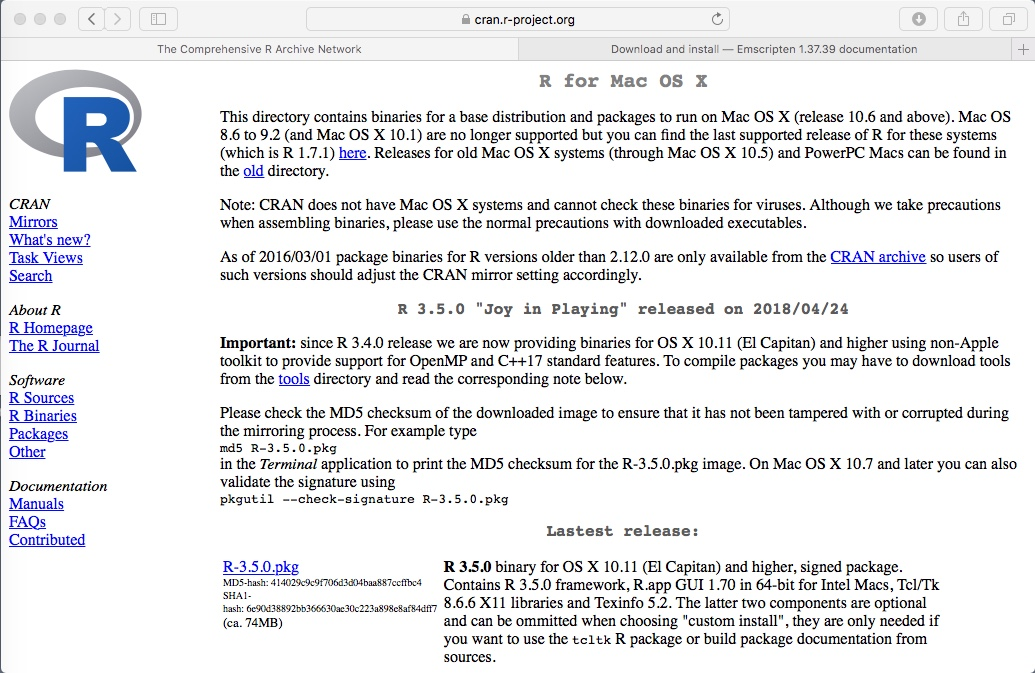
\includegraphics[width=5in]{./1-Introduction/SelectOS-Mac.jpeg} 
   \caption{Select MacOS operating system link}
%   \label{fig:example}
\end{figure}

\begin{figure}[h!] %  figure placement: here, top, bottom, or page
   \centering
   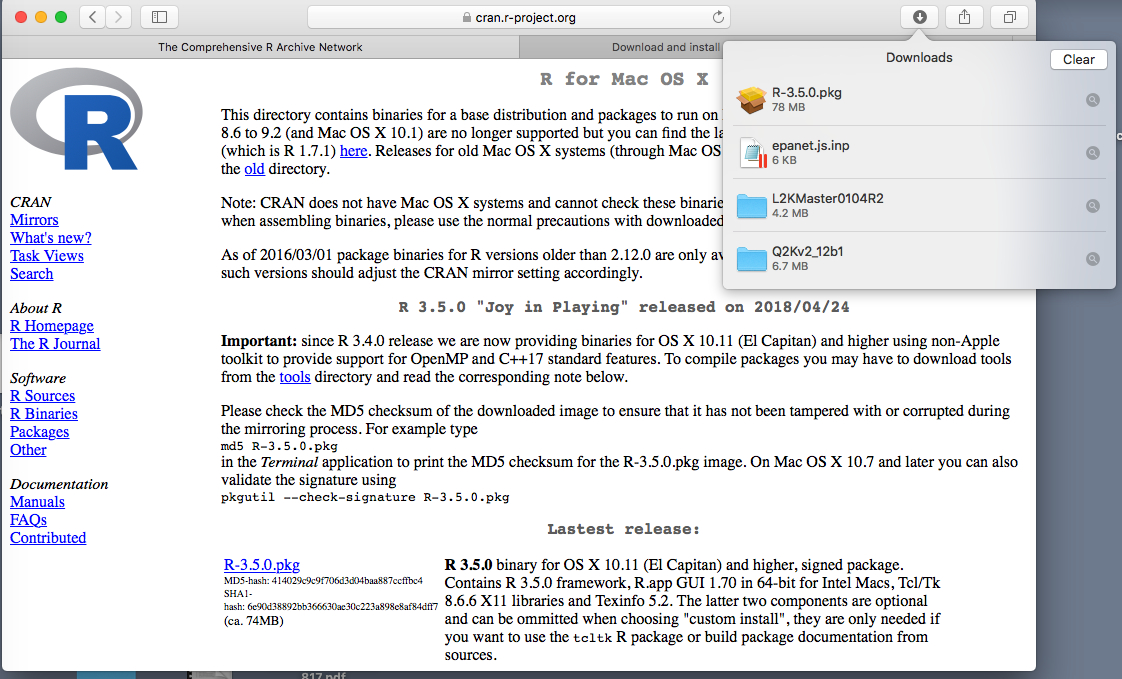
\includegraphics[width=5in]{./1-Introduction/DownloadR-pkg.jpg} 
   \caption{Download the R Installer}
%   \label{fig:example}
\end{figure}

\begin{figure}[h!] %  figure placement: here, top, bottom, or page
   \centering
   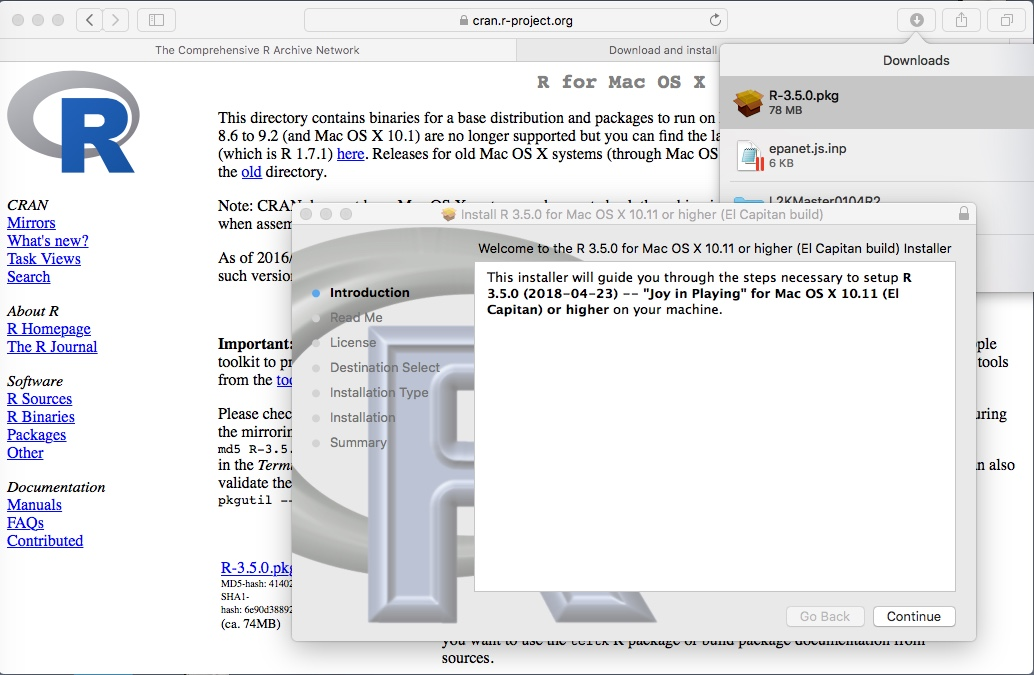
\includegraphics[width=5in]{./1-Introduction/RunInstallerMAC.jpeg} 
   \caption{Run the installer, accept the defaults}
%   \label{fig:example}
\end{figure}

\begin{figure}[h!] %  figure placement: here, top, bottom, or page
   \centering
   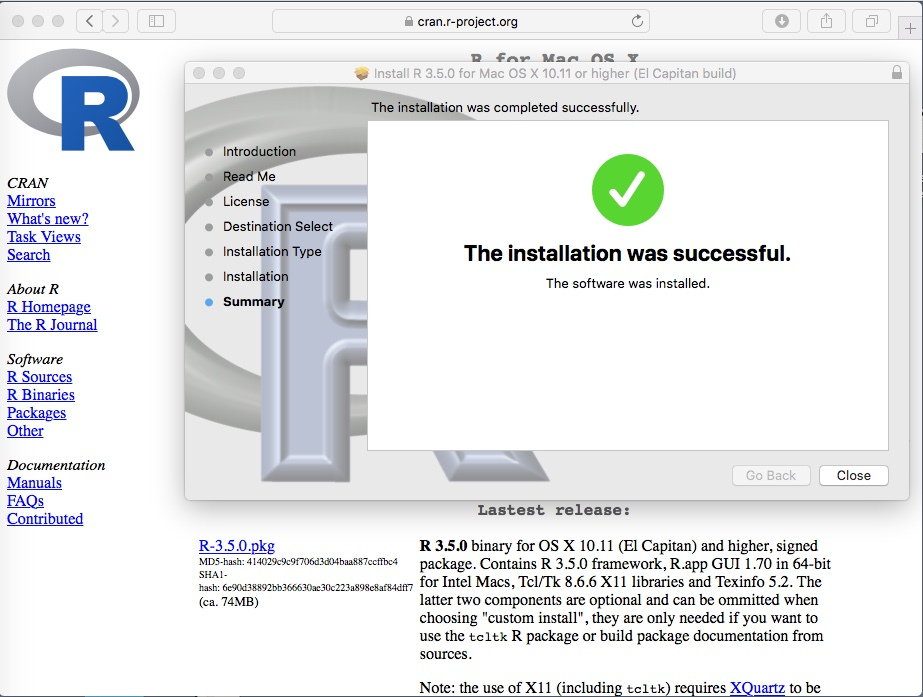
\includegraphics[width=5in]{./1-Introduction/MacSuccessR.jpeg} 
   \caption{Successful install}
%   \label{fig:example}
\end{figure}

\begin{figure}[h!] %  figure placement: here, top, bottom, or page
   \centering
   
\includegraphics[width=5in]{./1-Introduction/GoogleRStudio4Mac.jpeg} 
   \caption{Google R Studio}
%   \label{fig:example}
\end{figure}

\begin{figure}[h!] %  figure placement: here, top, bottom, or page
   \centering
   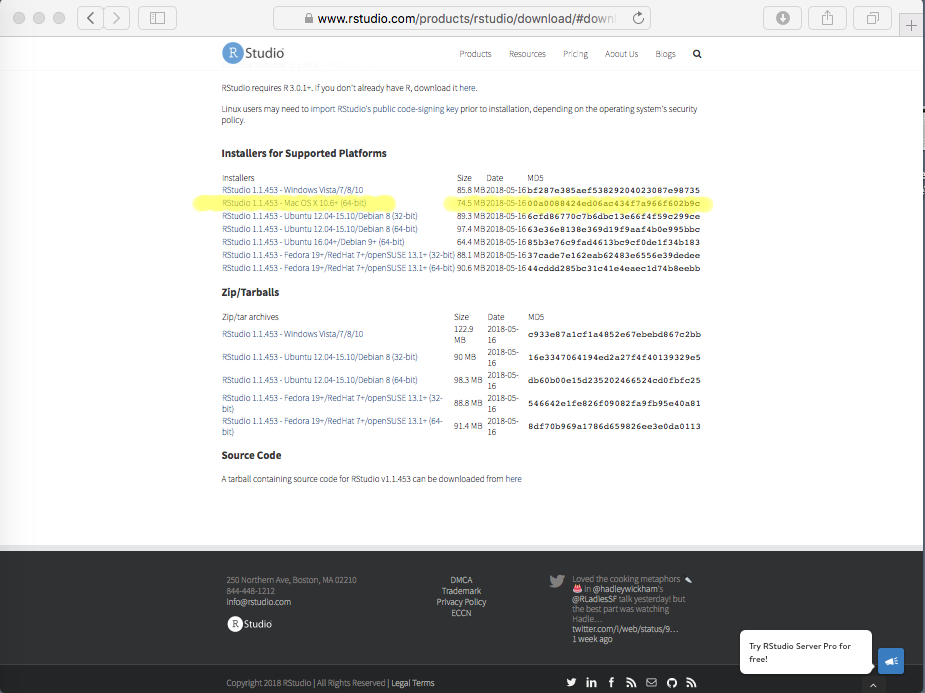
\includegraphics[width=5in]{./1-Introduction/SelectRStudioInstaller.jpg} 
   \caption{Select R Studio installer (for MacOS)}
%   \label{fig:example}
\end{figure}

\begin{figure}[h!] %  figure placement: here, top, bottom, or page
   \centering
   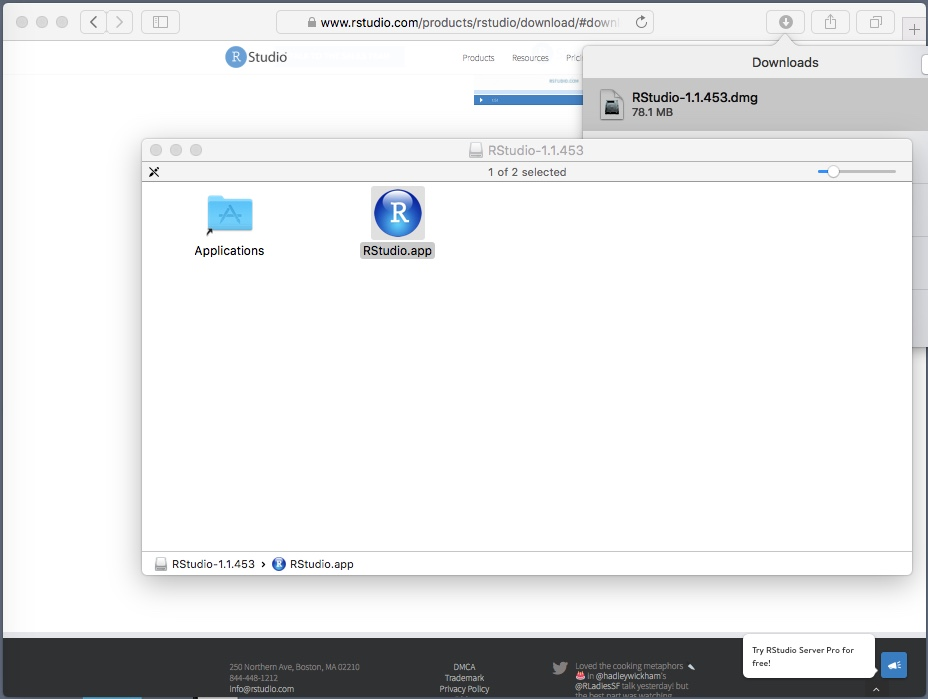
\includegraphics[width=5in]{./1-Introduction/MountDiskImage.jpeg} 
   \caption{Mount the disk image.  Then drag the R Studio icon on top of the Applications link -- this action will install the program}
%   \label{fig:example}
\end{figure}

\begin{figure}[h!] %  figure placement: here, top, bottom, or page
   \centering
   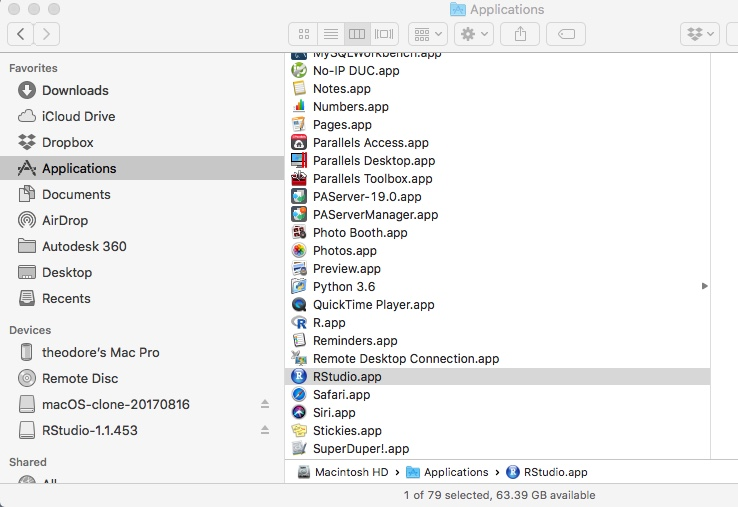
\includegraphics[width=5in]{./1-Introduction/LaunchRStudioMac.jpeg} 
   \caption{Start R Studio (in Applications directory, double click on the icon)}
%   \label{fig:example}
\end{figure}

\begin{figure}[h!] %  figure placement: here, top, bottom, or page
   \centering
   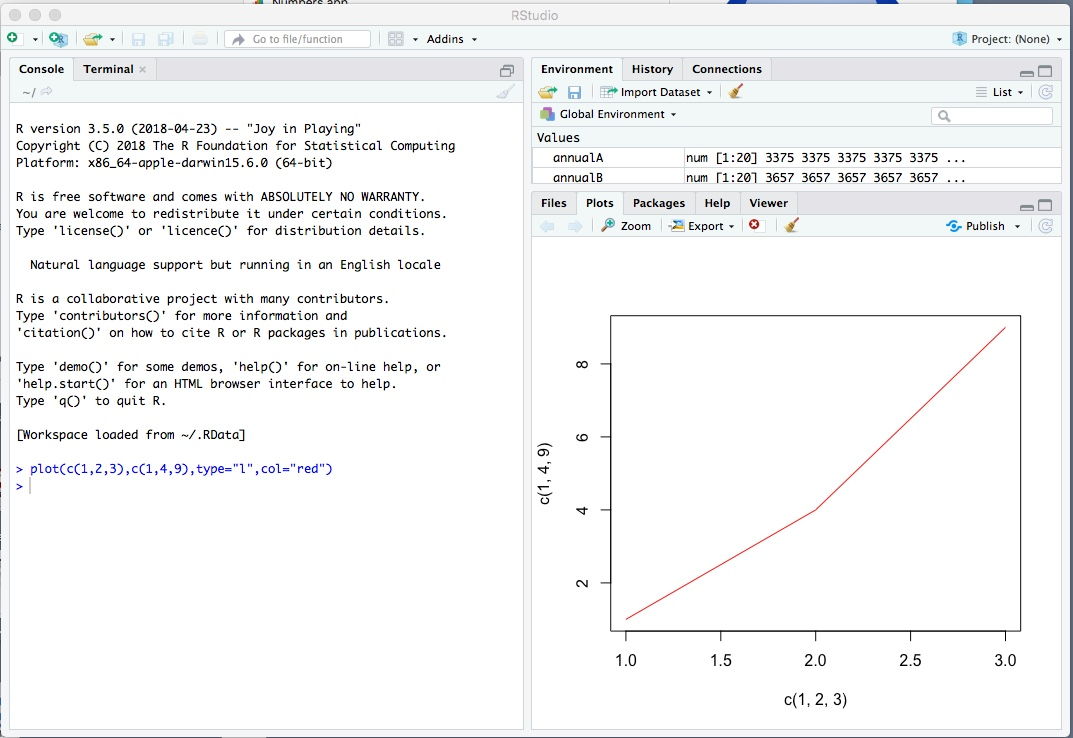
\includegraphics[width=5in]{./1-Introduction/TestMacInstall.jpeg} 
   \caption{Type in some R script and viola -- it produces a simple plot}
%   \label{fig:example}
\end{figure}

\newpage~
\newpage~
\newpage~
\newpage~
\newpage~
Yipee!  It is running.  You can install additional packages now or later.  You should now have sufficient computation capability for the course.  



\clearpage
\subsubsection{Linux Users}
The purpose of this section is to demonstrate how to get \textbf{R} and \textbf{R Studio}  running on a Linux computer.  
This document assumes the following:
\begin{enumerate}
\item You have internet connection.
\item You have sufficient user privileges to install software on your machine.  
Generally, if it is your own machine then you have superuser (root) privileges.
If it is some network machine maintained by someone else you probably don't have such priviliges.
The examples here use the \texttt{sudo <command>} to do the installs -- on my machine the password I enter is my user password (and not the root password).  
Alternativley you can switch user \texttt{su} to root, and run the installs as root -- this approach is considerably more dangerous in terms of wrecking your operating system that using the \texttt{sudo} approach.
\item You have 60MB or so of vacant disk space on the system directory.
\end{enumerate}

The step-by-step guide is presented as a series of screen captures.  Obviously adjust inputs to fit your machine.  
Use the most recent, stable version offered on CRAN (Comprehensive R Archive Network).

\begin{figure}[h!] %  figure placement: here, top, bottom, or page
   \centering
   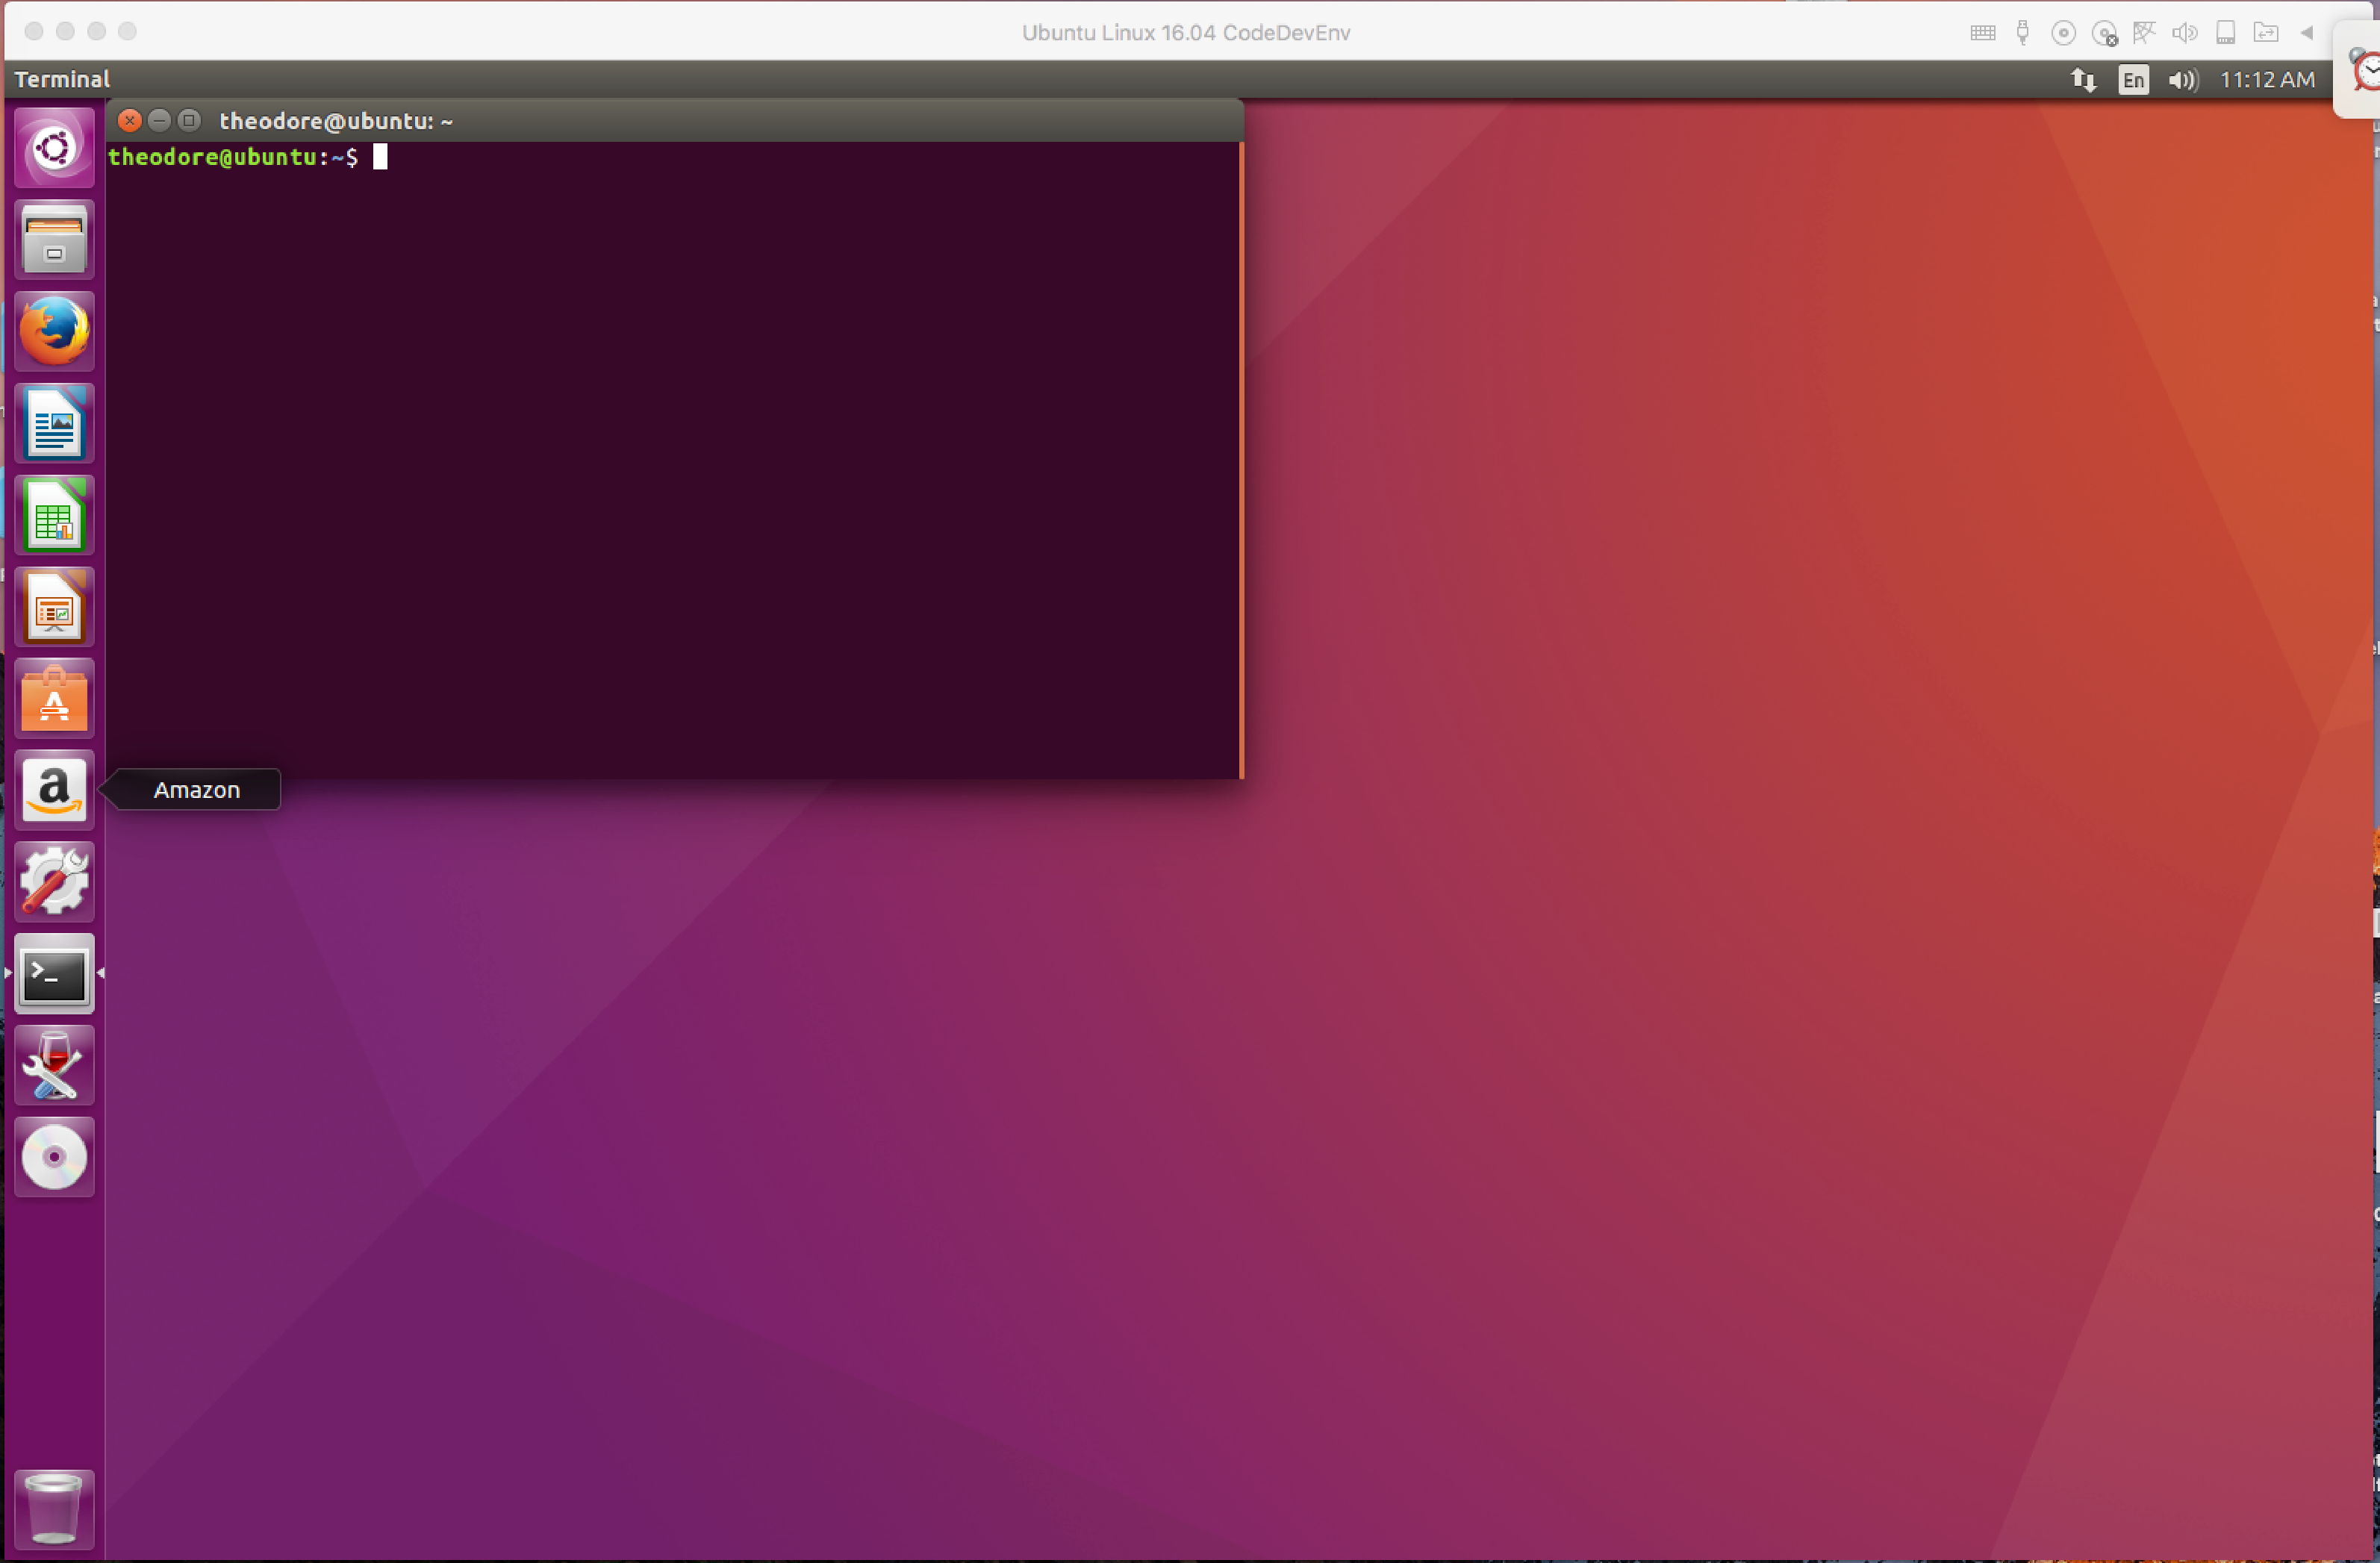
\includegraphics[width=5in]{./1-Introduction/LinuxTerminalPrompt.pdf} 
   \caption{Terminal Prompt in Linux}
%   \label{fig:example}
\end{figure}

To get started we need to install \textbf{R}.  
The easiest method is to use the package manager -- my Linux distribution is Ubuntu 16.XX.  
It is built from the debian distribution and uses the \texttt{apt} package manager.
The package manager is pretty cool because when we request a package it finds the package and its dependencies, downloads everything needed and then we can install.
In earlier times (the 1990's) using the Red Hat Package Manager (\texttt{rpm}) one would have to find the dependencies themselves (in all fairness \texttt{rpm} would identify the dependencies and suggest where to find them!).  So here we go, first open a terminal in Linux.

Next in the terminal window issue the command \texttt{sudo apt install r-cran-littler}.

\begin{figure}[h!] %  figure placement: here, top, bottom, or page
   \centering
   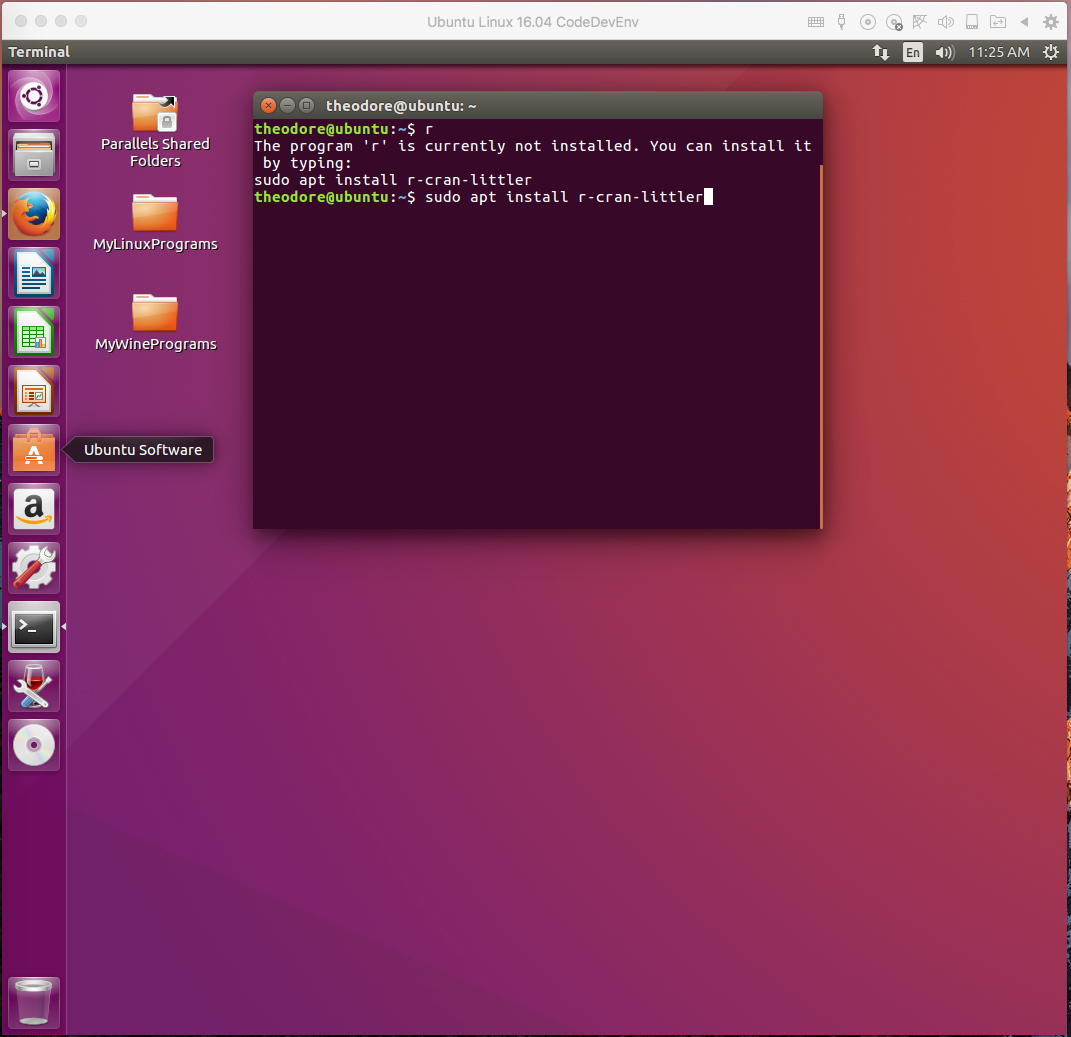
\includegraphics[width=4.5in]{./1-Introduction/LinuxInstallR.jpg} 
   \caption{Install R using the \texttt{apt} package manager (or \texttt{rpm} if using a red hat variant)}
%   \label{fig:example}
\end{figure}

When you press return, the computer should ask for a password -- use your user password; if you have install privileges this will work.  
If not, you will have to switch user to root and either add your user account to the group \texttt{wheel}, return to your account -- or just install as root.

Next the install will begin and may take a few minutes.  
Usually there is a lot of installer messages that run across the screen (kind of like in ``The Matrix'').
The \texttt{apt} utility is downloading files and binging them to resources on the system so that \textbf{R} can run.
Eventually it should get to the end of the install and may look something like the next screen capture.

Our next task is to verify that the install was successful.
Usually failure is obvious, but not always.
I find the easiest way to verify that the operating system thinks the software is installed is issue the command to run the program with the version switch active.
In this case, issue the command \texttt{r --version}.
This command will try to run \textbf{R}, and will return the version number (or build number). 

In the next screen capture when we run the command we see that the version number is \textbf{R} version 3.2.2.
The version numbering system is typical for all software -- it identifies something like this is the second subversion, of the second revision, of the third stable release. 

\begin{figure}[h!] %  figure placement: here, top, bottom, or page
   \centering
   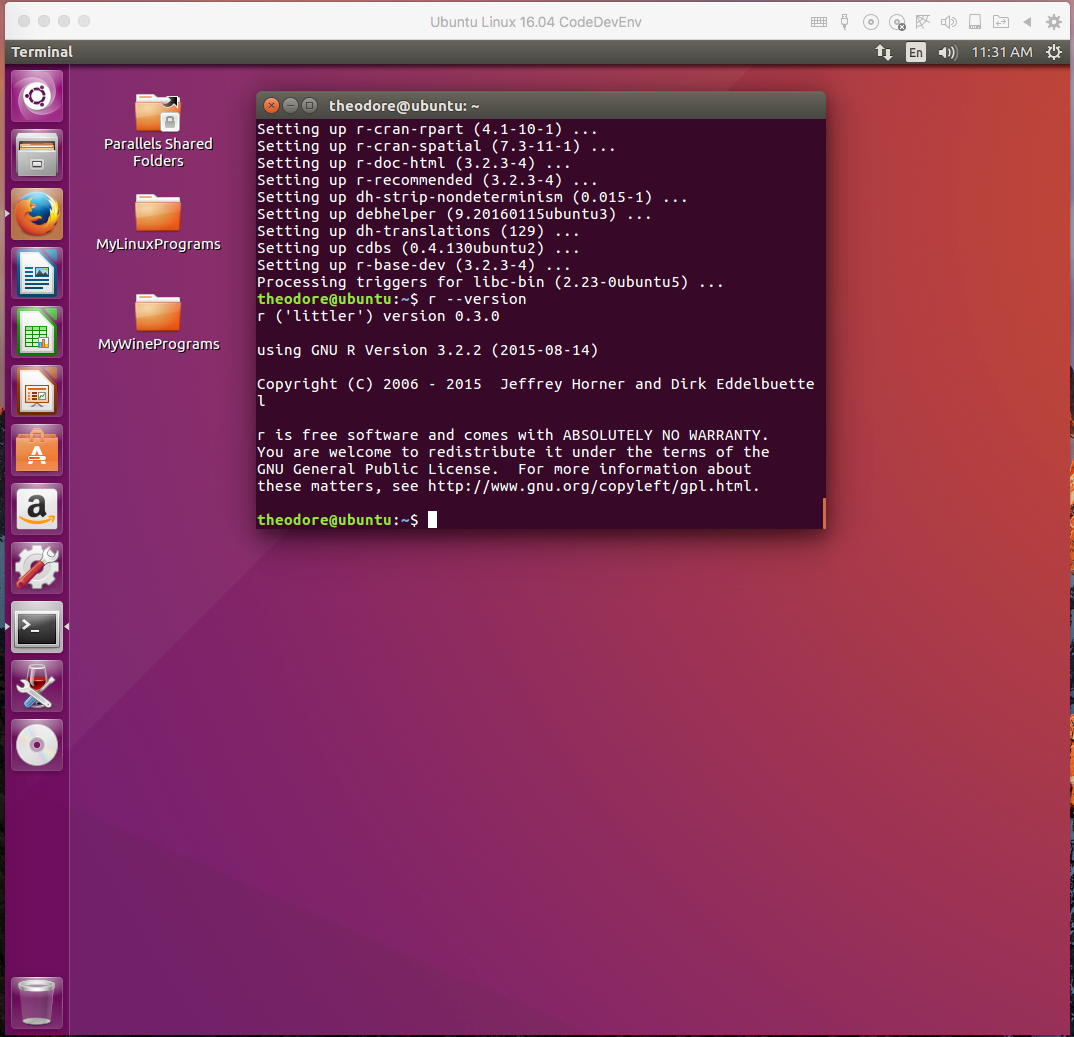
\includegraphics[width=5in]{./1-Introduction/LinuxRVersion.jpg} 
   \caption{Verify install of \textbf{R} using \texttt{r --version}}
%   \label{fig:example}
\end{figure}

The next step I recommend is to go ahead and download a development environment.
\textbf{R Studio} is an integrated development environment for \textbf{R}.   
We don't ``need'' it, but it enforces some discipline, gives us a place to store and modify \textbf{R}-scripts (little programs), and lets us see all of our work going on in one location.

To get \textbf{R Studio} we have to download it from the manufacturer, the copy we will use is free.  
Instead of \texttt{apt} this time I used Firefox to navigate to the \textbf{R Studio} website, then select download.

Next select the appropriate installer for your platform.
Be sure you are selecting an installer and not the source codes for the program.\footnote{In theory we could build the program from source using the make utility and (hopefully) already installed compilers -- this is for people with time, training, inclination and need.  We are going to use the already built binaries!}

We will download the 64-bit version (unless you have a 32-bit machine, then you need 32-bit software).
We need to select our Linux platform -- mine is Unbuntu/Debian.   
I also have a Red Hat/SuSe machine, so if I were using that machine, i would select its software.

\begin{figure}[h!] %  figure placement: here, top, bottom, or page
   \centering
   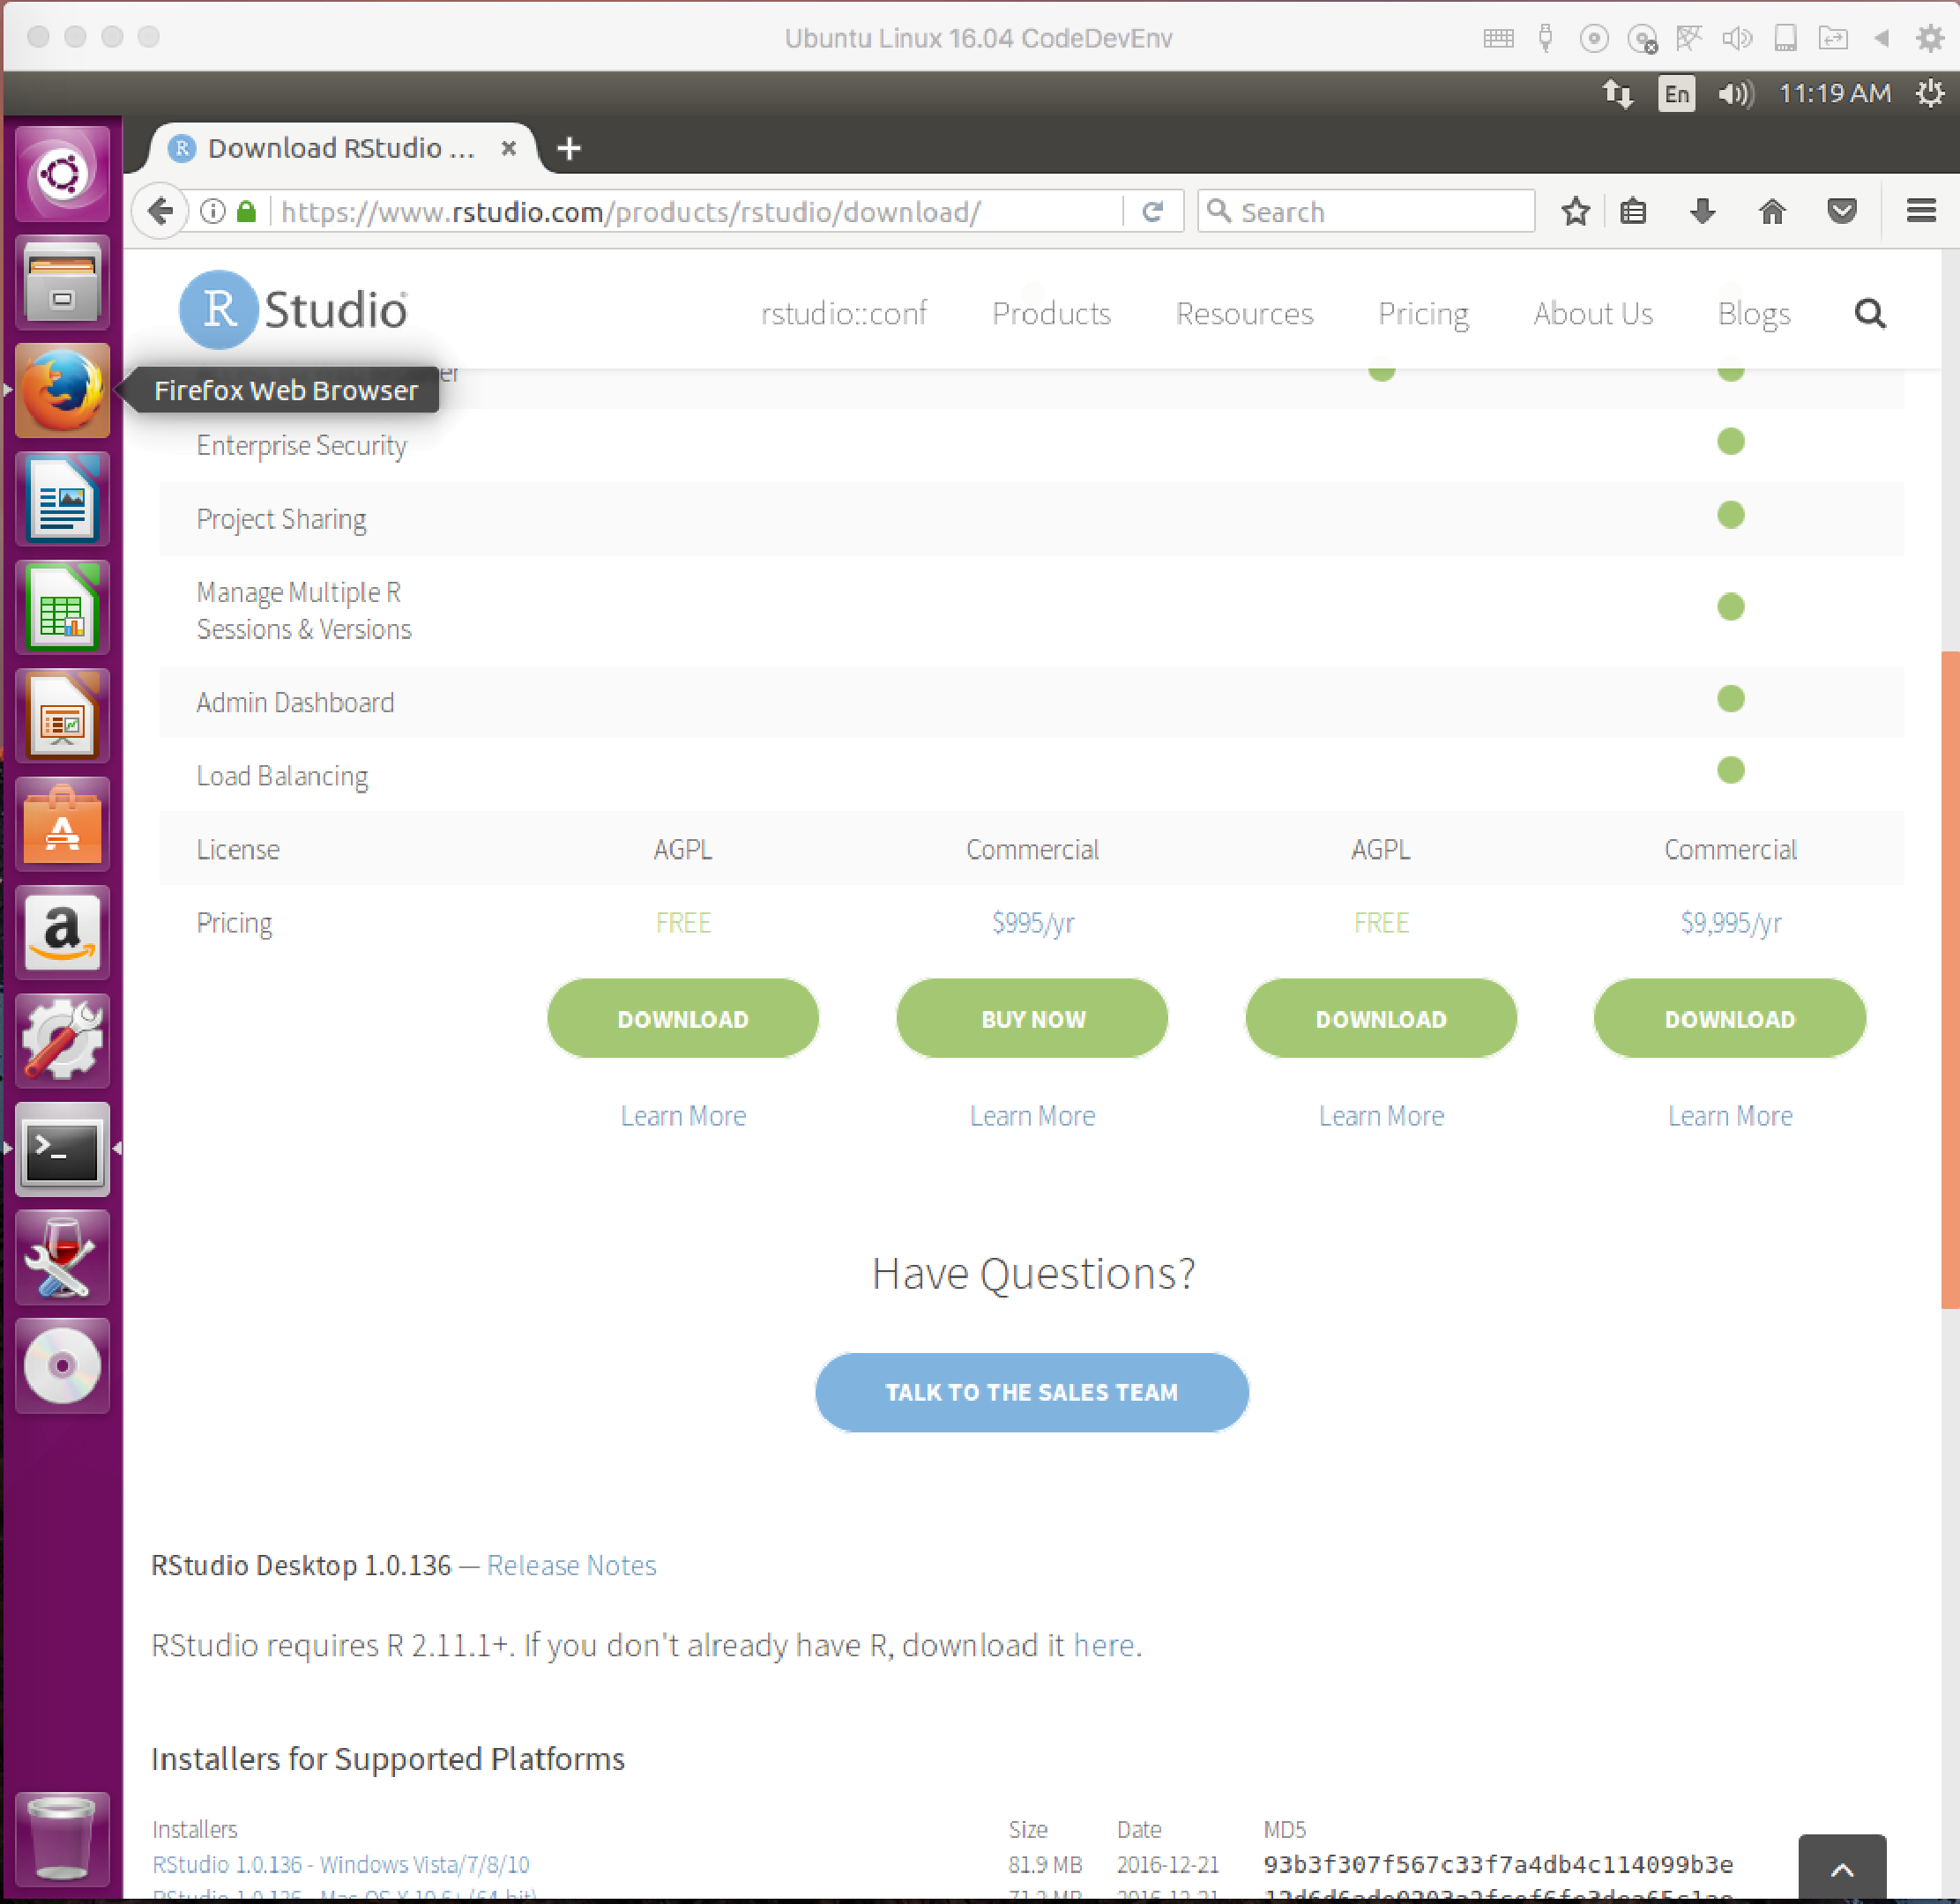
\includegraphics[width=3.5in]{./1-Introduction/LinuxRStudio.pdf} 
   \caption{Browser search for \textbf{R Studio}; go to downloads.  We are going to select the free (leftmost) column}
%   \label{fig:example}
\end{figure}

\begin{figure}[h!] %  figure placement: here, top, bottom, or page
   \centering
   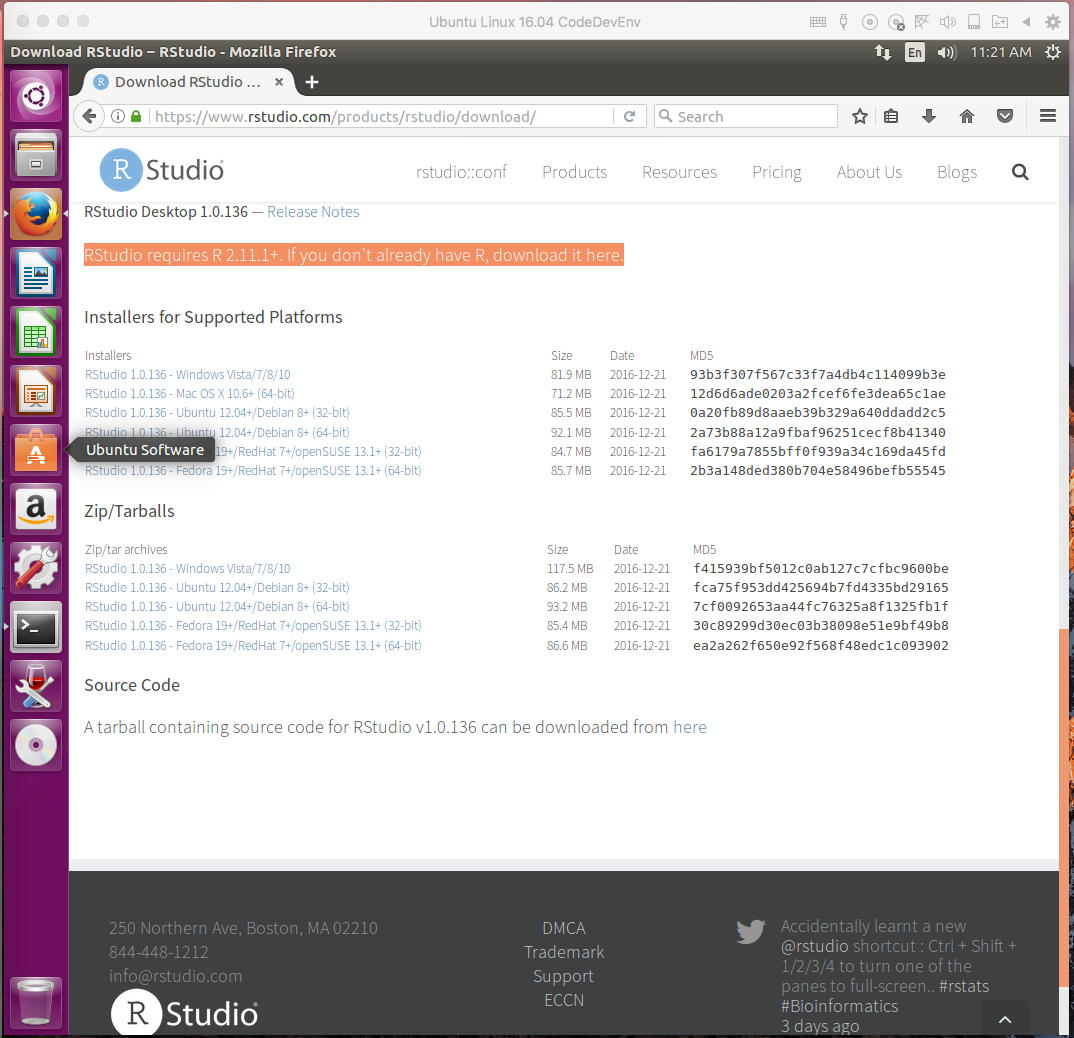
\includegraphics[width=3.5in]{./1-Introduction/LinuxRStudioDownload.jpg} 
   \caption{Download the version of \textbf{R Studio}; in this case 64-bit for Ubuntu Linux (what I am using).  
   My computer asks if upon download if I want to run the installer, of course select YES}
   \label{fig:LinuxRStudioDownload}
\end{figure}

\clearpage

Figure \ref{fig:LinuxRStudioDownload} is the selection page for selecting the installers.  
Once I select the package the computer starts the download, and asks me if I want to run the installer, as in Figure \ref{fig:LinuxRStudioInstall}



\begin{figure}[h!] %  figure placement: here, top, bottom, or page
   \centering
   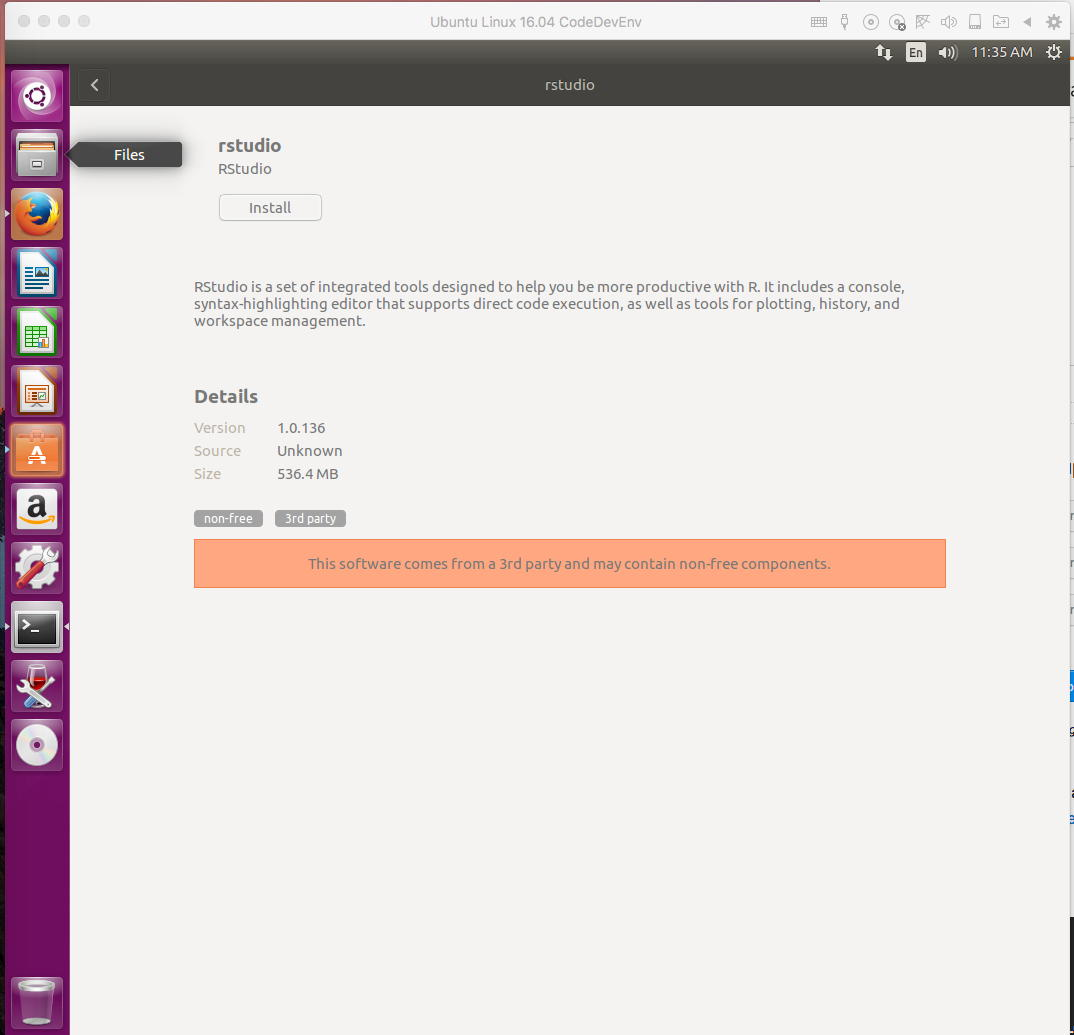
\includegraphics[width=3.5in]{./1-Introduction/LinuxRStudioInstall.jpg} 
   \caption{Here we select install, and let the installer do its thing}
   \label{fig:LinuxRStudioInstall}
\end{figure}

Selecting yes, the installer will attempt to install \textbf{R Studio} onto my computer. 
Once installation is complete, the program is ready for a validation (of install) run.

\begin{figure}[h!] %  figure placement: here, top, bottom, or page
   \centering
   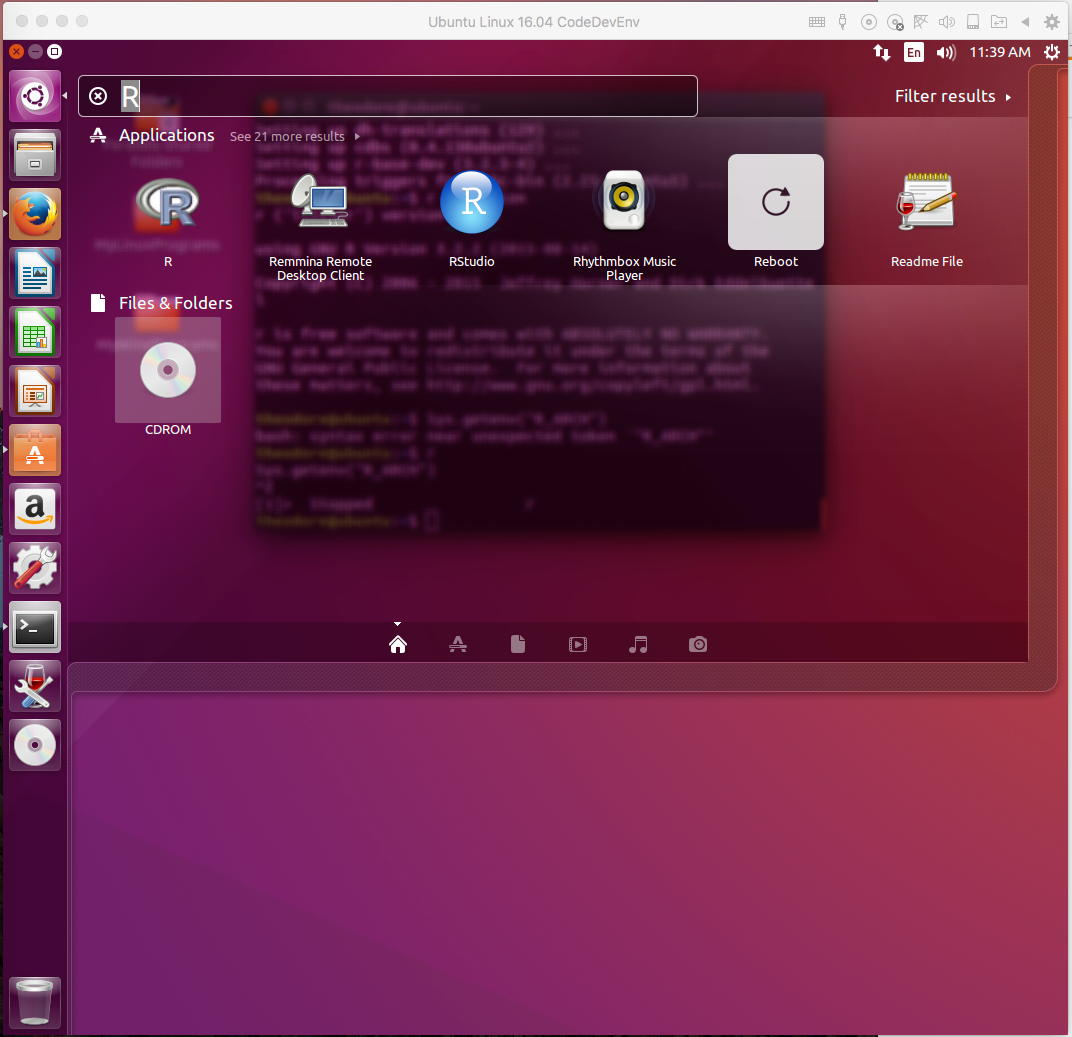
\includegraphics[width=3.35in]{./1-Introduction/LinuxRStudioSelect.jpg} 
   \caption{To launch \textbf{R Studio}, either select in the applications folder (or type in the terminal \texttt{rstudio}}
\label{fig:LinuxRStudioSelect}
\end{figure}

\clearpage
Figure \ref{fig:LinuxRStudioSelect} is a screen capture after installation using the Unbuntu program manager window.  
Both \textbf{R} and \textbf{R Studio} are available.  

Either select \textbf{R Studio} to launch it, or type in a terminal window \texttt{rstudio} and the IDE should launch.
The IDE itself is a bit complicated, but actually enables us to keep better track of our work and ultimately saves time.
MatLab users should notice that the interface looks quite similar (at least it does to me) -- its also the same concept.

Figure \ref{fig:LinuxRStudioOpen} is the result of launching the program.  
The left side of the IDE is an \textbf{R} console -- exactly what would occur if we had just started \textbf{R}.
The right side of the IDE is divided into an upper and lower panel.  
Each panel  provides information about our programming environment at any instant -- and the content is selectable from the icons at the top of each panel.


\begin{figure}[h!] %  figure placement: here, top, bottom, or page
   \centering
   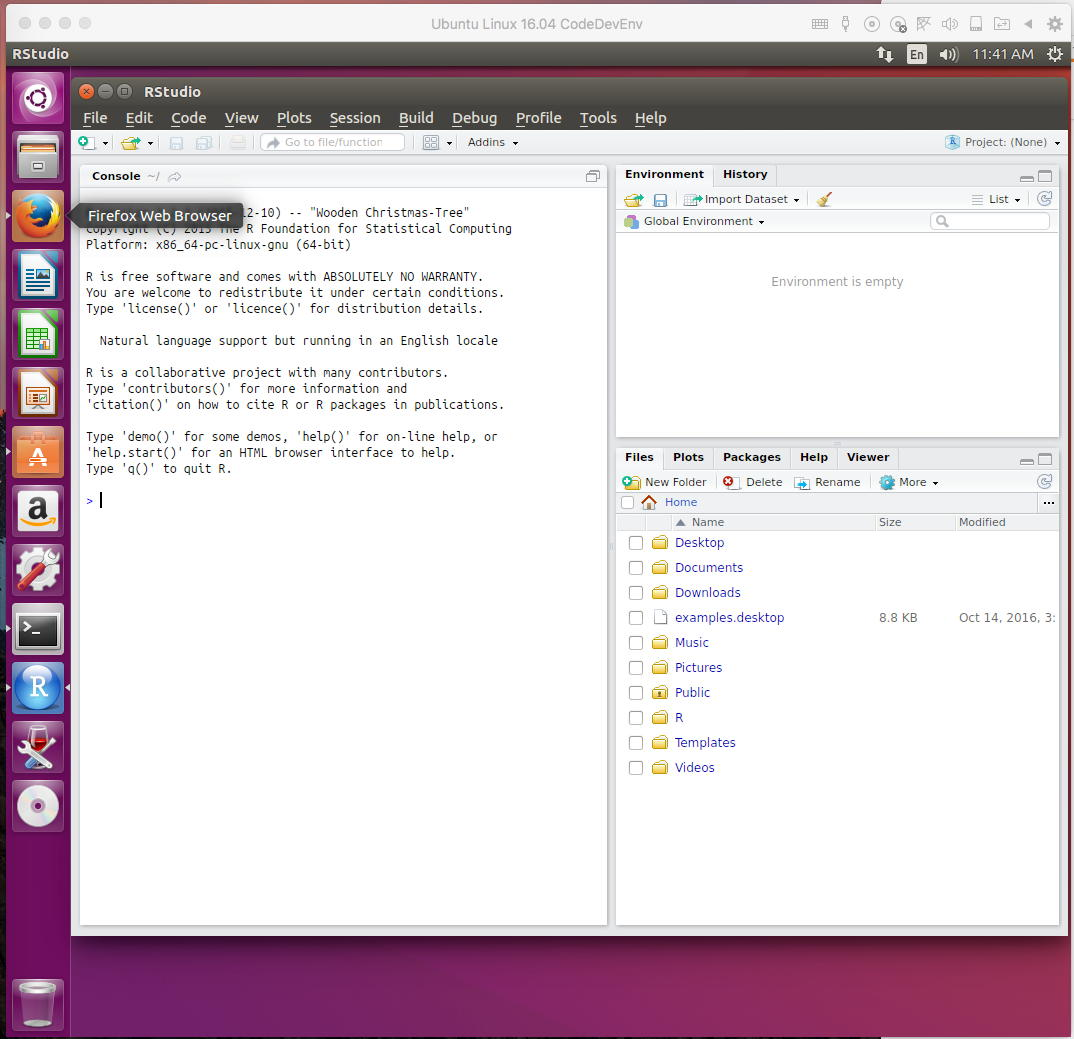
\includegraphics[width=4.5in]{./1-Introduction/LinuxRStudioOpen.jpg} 
   \caption{Upon opening you should have the following integrated development environment (IDE).   The left panel is exactly what you would obtain if
   you just type \texttt{r} in the terminal window.  }
   \label{fig:LinuxRStudioOpen}
\end{figure}

The next few figures are a step-by-step example to introduce \textbf{R Studio} as well as test if it installed correctly.
We could simply type in the \textbf{R} console within the IDE, but instead to get into the habit of saving our work, we will open a new scripting file.
\clearpage

Figure \ref{fig:LinuxRStudioNewFile} shows the process of selecting FILE/OPEN to create a new file to store our scripts.
We will type a few commands into the file and then run them.

\begin{figure}[h!] %  figure placement: here, top, bottom, or page
   \centering
   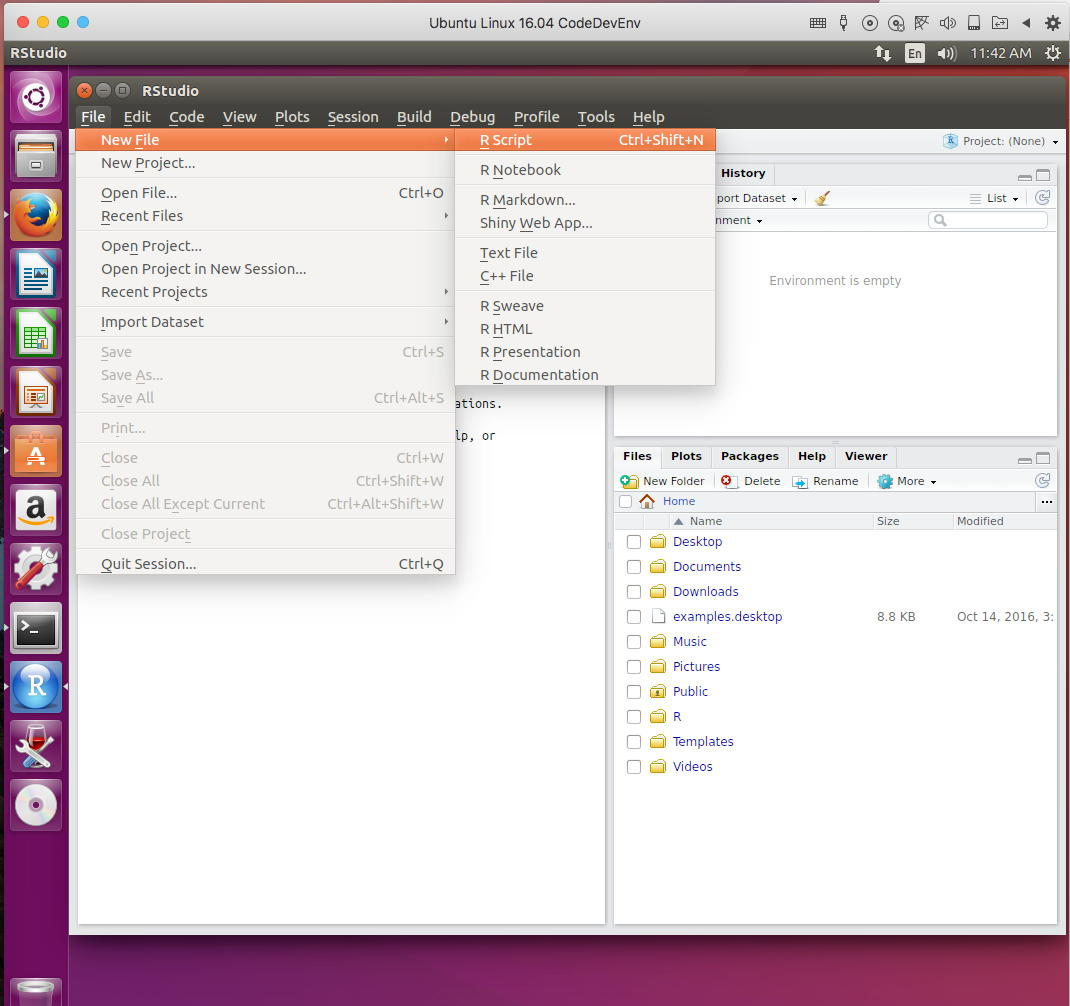
\includegraphics[width=4in]{./1-Introduction/LinuxRStudioNewFile.jpg} 
   \caption{Open a new file -- in this case as an \textbf{R-Script}}
   \label{fig:LinuxRStudioNewFile}
\end{figure}

\begin{figure}[h!] %  figure placement: here, top, bottom, or page
   \centering
   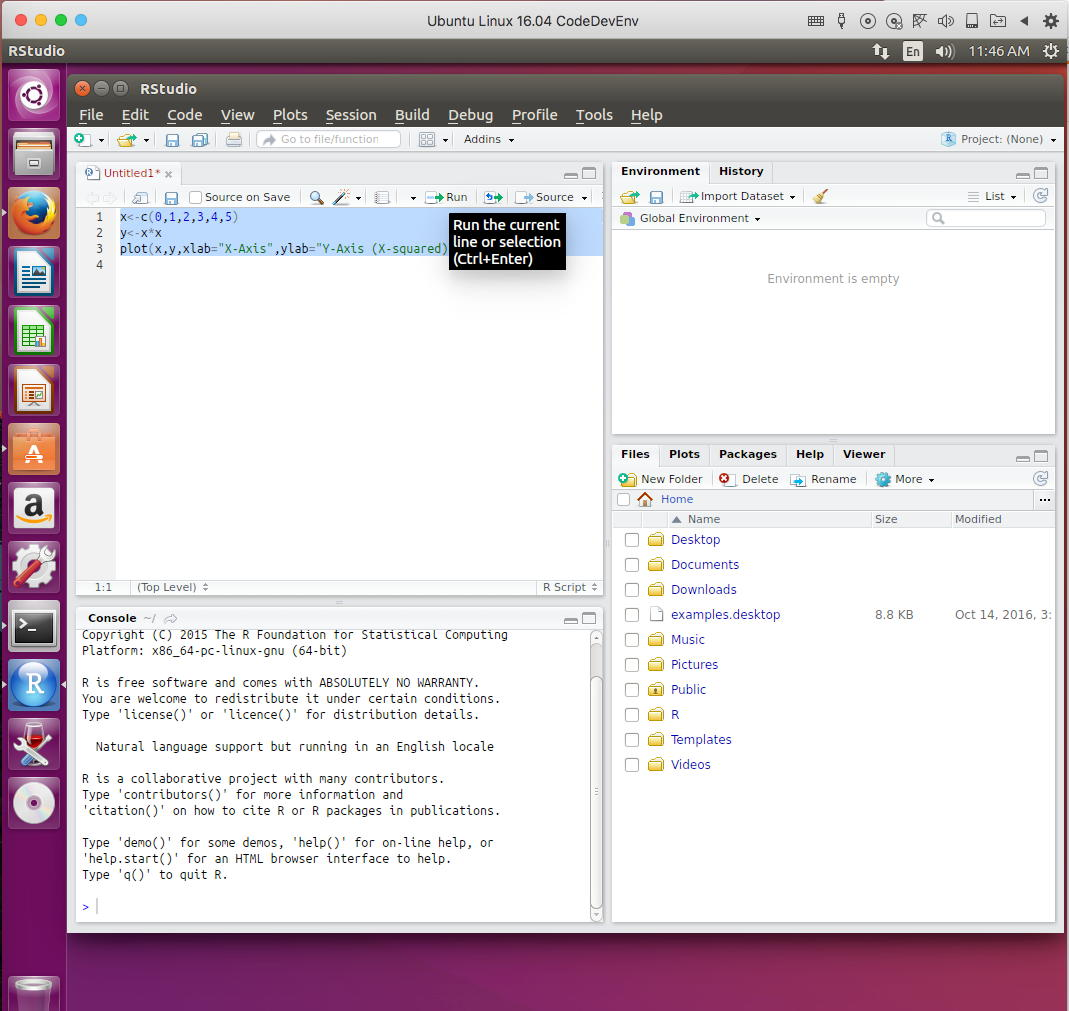
\includegraphics[width=4in]{./1-Introduction/LinuxRStudioRunFile.jpg} 
   \caption{Type in some \textbf{R} instructions, select the instructions and choose \texttt{RUN}}
   \label{fig:LinuxRStudioRunFile}
\end{figure}

So once the file is open the left side of the IDE divides into two panels, an upper and lower panel.
The lower panel is the console environment, and the upper panel is a script editor.

Figure \ref{fig:LinuxRStudioRunFile} shows the upper panel with the \textbf{R} commands shown in Listing \ref{lst:LinuxRStudioRunFile}

\begin{lstlisting}[caption=R code demonstrating a few commands \\ This fragment of code generates two vectors X and Y and then plots them, label=lst:LinuxRStudioRunFile]
############### Some R Commands ########################
x <- c(0,1,2,3,4,5) # create a vector of 6 elements -- integers 0 to 5.
y <- x*x                 # square x, put result in y.
plot(x,y,xlab="X_Axis",ylab="Y-Axis (X-squared)",lwd=3, type="l") # make and label a plot
\end{lstlisting}  

To actually run the code we can either highlight the portion of the script file we wish the program to execute (that's what done here), or we can save the file and run the entire file.
Often we will do both -- highlight portions to develop a model, then save and run the file as needed.
The term ``sourcing'' a [file] in \text{R} is jargon for running the commands contained within a file named [file].
The ability to save and reuse commands is really useful and is what makes \textbf{R} (or any other stored program software) really useful.

Figure \ref{fig:LinuxRStudioCompleted}  is the result of highlighting these three lines of code and running them (notice the little run icon above the script editor).

\begin{figure}[h!] %  figure placement: here, top, bottom, or page
   \centering
   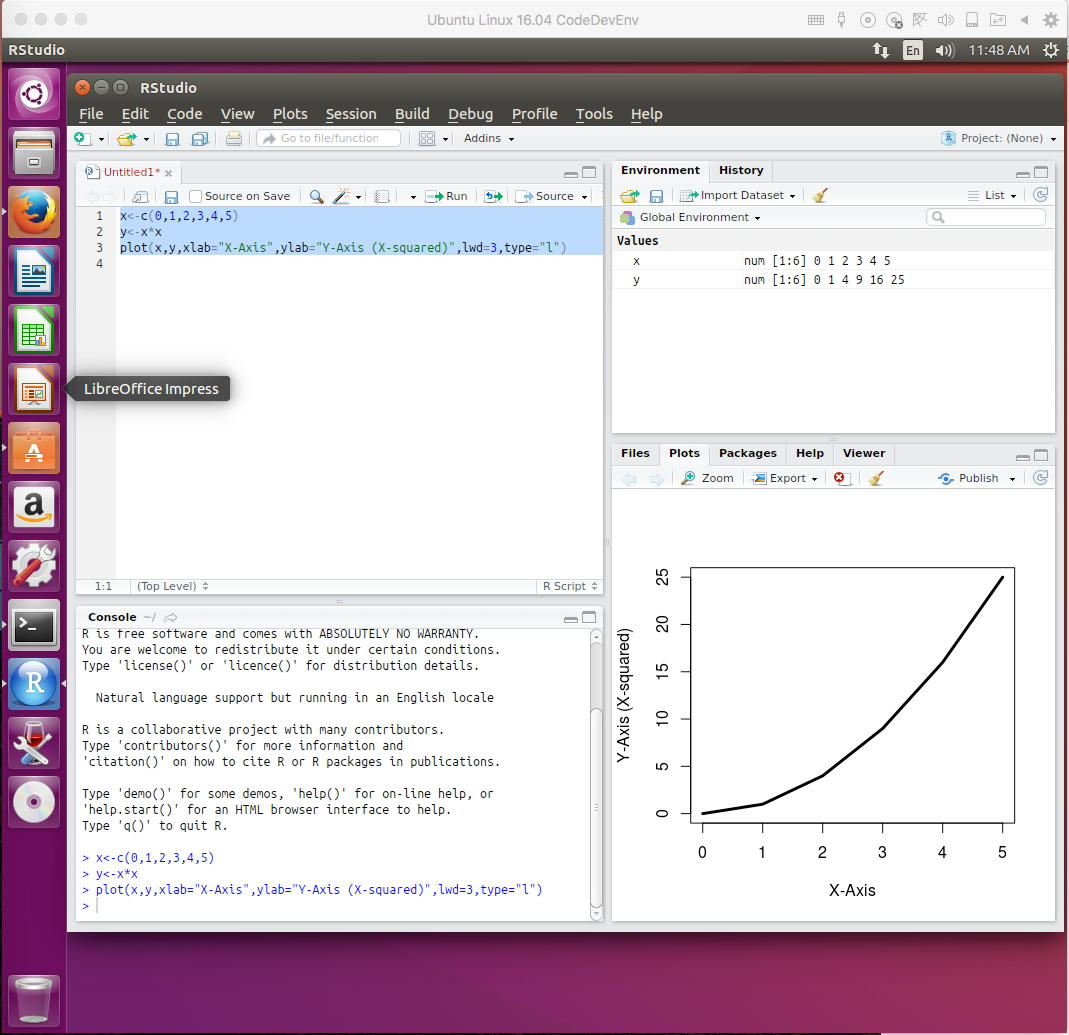
\includegraphics[width=4.5in]{./1-Introduction/LinuxRStudioCompleted.jpg} 
   \caption{Completed script run.  Notice the plot in the lower right panel.  At this point you have a functioning programming tool}
   \label{fig:LinuxRStudioCompleted}
\end{figure}

\clearpage

%\subsection{Exercises}

%%%%%%%%%%%%%%%%%%%%%%%%%%%%%%%%%%%%%%%%%%%%%%%%%%%%%%%%%%%%%%
%%%%%%%%%%%%%%%%%%%%%%%%%%%%%%%%%%%%%%%%
%\section{Algorithms and \textbf{R} for Computing}
An algorithm is a recipe.  A useful definition is 
\begin{quote}
An algorithm is a computational method or an ensemble of rules determining the order and form of numerical operations to be applied to a set of data $\textbf{a}(a_1,a_2,\dots)$ in order to find a new set of values $\textbf{x}(x_1,x_2,\dots)$ forming the solution of a problem.

An algorithmic procedure can be represented as 
\begin{equation}
\textbf{x}~=~f(\textbf{a})
\end{equation}

From a mathematical perspective the main concern is that the algorithm is well posed:
\begin{enumerate}
\item A solution exists for a given $\textbf{a}$.
\item The computation must lead to a single solution for $\textbf{x}$ given $\textbf{a}$.
\item The results for $\textbf{x}$ must be connected to the input $\textbf{a}$ through the Lipschitz relation.
\begin{equation}
|\delta \textbf{a}| < \eta~~\text{then}~~ |\delta \textbf{x}| < M|\delta \textbf{a}|
\end{equation}
where $M$ is a bounded natural number, $M = M(\textbf{a},\eta)$\footnote{Think of $M$ as a mapping function.}.
\end{enumerate}

Certain common problems are not well posed as stated but with reasonable assumptions can be forced into such a state.
\end{quote}

Thus an algorithm is a recipe to take input data and produce output responses through some relationships.  If a well posed problem then each result is related to the inputs, and the same inputs (in an algorithm) produce the same results.  By the recipe analogy, if you follow the same recipe each time with the same raw materials then the cake should taste the same when it is baked.

An important concept is that an algorithm operates on data (procedure-oriented); an object-oriented view is that an algorithm performs a task (generate response) based on states established by the data.  Both points of view are valid and equivalent.

Most computational hydraulics models are built (by a quirk of history) in a procedure-oriented perspective.
%Need more here

\subsection{Tools}
A practicing modeler needs a toolkit --- these tools range from the actual computation engine (EPA-SWMM, HEC-RAS, FESWMS, HSPF, WSPRO, TR-20, etc.) to analysis tools for result interpretation (\textbf{R}, \textbf{Excel}) to actual programming tools (\texttt{FORTRAN},\texttt{PERL}, etc.) to construct their own special purpose models or to test results from general purpose professional models.

In this book \textbf{R} will be used for programming, analysis, and presentation.  

\subsection{Programming}
Why programming?

There are three fundamental reasons for requiring a programming experience:
\begin{enumerate}
\item Teaching someone else a subject or procedure forces the teacher to have a reasonable understanding of the subject or procedure.  Teaching a computer (by virtue of programming) forces a very deep understanding of the underlying algorithm.  
\item You will encounter situations that general purpose programs are not designed to address; if you have a moderate ability to build your own tools when you need to, then you can.  In all likliehood, you will ``trick'' the professional program, but you cannot invent tricks unless you know a little bit about programming.
\item Programming a computer requires an algorithmic thought process --- this process is valuable in many other areas of engineering, hence the act of programming is good discipline for other problems you will encounter.
\end{enumerate}

%%%%%%%%%%%%%%%%%%%% CHAPTER 3 %%%%%%%%%%%%%%%%%%%%%%%%%%
%%%%% Variables and Operators %%%%%%%%%%%%%%%%%%%%%%%%%%%%%%%%%%% 
\subsection{Interpolating Tabular Data -- A useful algorithm}
Material properties in physical systems are usually tabulated values.
A frequent task is to interpolate in a set of tabular values to approximate the value between rows (or columns) in the table.  
Linear interpolation is the common technique used; and the tables can are stores as either separate files, or, if the tables are small enough, they can be directly imbedded into the code.

\subsection{Linear Interpolation}
Figure \ref{fig:XYPair} is a sketch of a set of ordered pairs $(x,y)$. 

\begin{figure}[h!] %  figure placement: here, top, bottom, or page
   \centering
   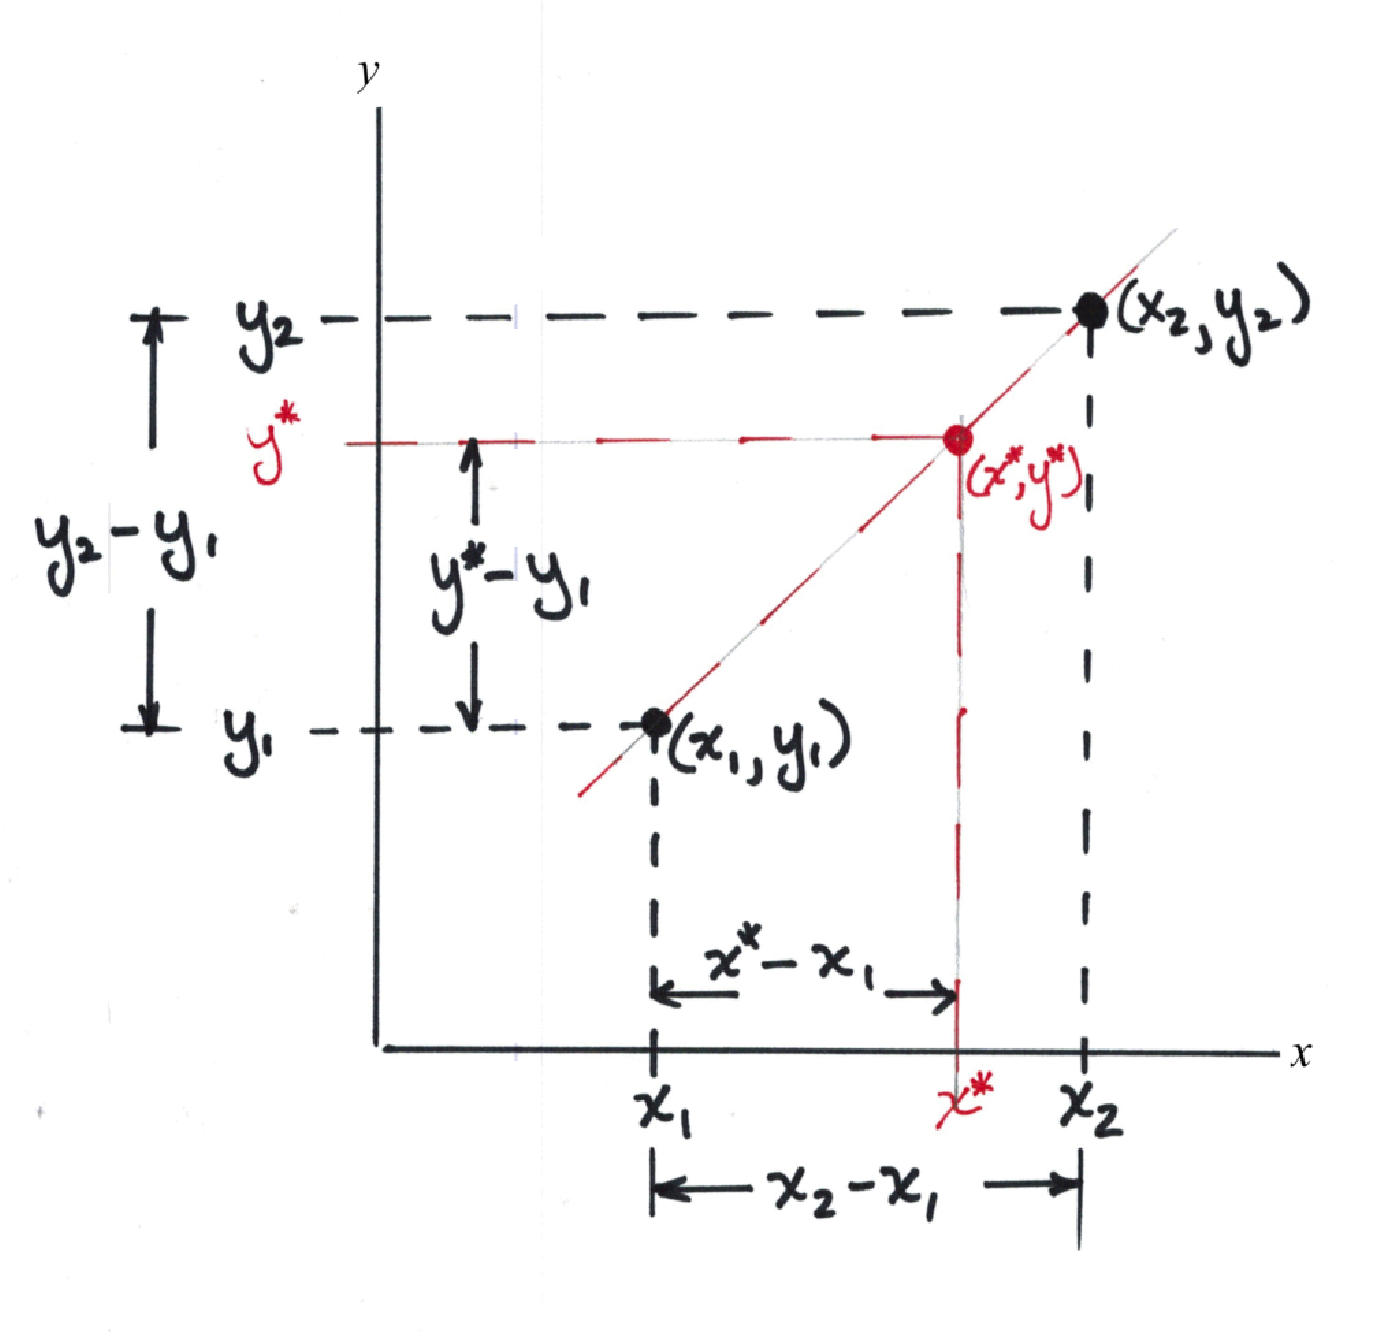
\includegraphics[width=6in]{./2-Algorithms/XYPair.jpg} 
   \caption{Sketch of two adjacent values from a table, plotted in Cartesian coordinate system.}
   \label{fig:XYPair}
\end{figure}

These pairs (there are two in the sketch) represent values in a table, for instance $x$ may represent water temperature, and $y$ may represent vapor pressure at that particular temperature.
Two adjacent values (in the table) are depicted in the sketch, and the pairs are ordered bases on the $x$-value.  

Now suppose we want to estimate the value of $y^*$ at some intermediate value $x^*$ that lies between $x_1$ and $x_2$.
As a computational task, the problem statement is to\\~\\
``Estimate the value of $y^*$ associated with the value $x^*$ given the ordered pairs $(x_1,y_1)$ and $(x_2,y_2)$.'' \\~\\
Linear interpolation simply uses the concept of similar triangles to scale the $x$ and $y$ distances between the ordered pairs to the intermediate location.   Equation \ref{eqn:InterpolationEquation} is the result of application of similar triangles to the situation described by Figure \ref{fig:LinearInterpolation} and the problem statement.

\begin{equation}
\frac{x^*-x_1}{x_2-x_1}=\frac{y^*-y_1}{y_2-y_1}
\label{eqn:InterpolationEquation}
\end{equation}

Next, apply algebra to solve Equation \ref{eqn:InterpolationEquation} for $y^*$, to obtain Equation \ref{eqn:InterpolationEquation2}

\begin{equation}
y^*=y_1+\frac{(y_2-y_1)(x^*-x_1)}{(x_2-x_1)}
\label{eqn:InterpolationEquation2}
\end{equation}

Now we can use \ref{eqn:InterpolationEquation2} to estimate values between any two data pairs.\\

\subsubsection{Interpolation of Values in Two Pairs}

Figure \ref{fig:FluidData} is a table of water properties from (CITE), that represents typically how tabular data are presented.  The temperature column is arranged in increasing order and the other properties associate with temperature across a row.

\begin{figure}[htbp] %  figure placement: here, top, bottom, or page
   \centering
   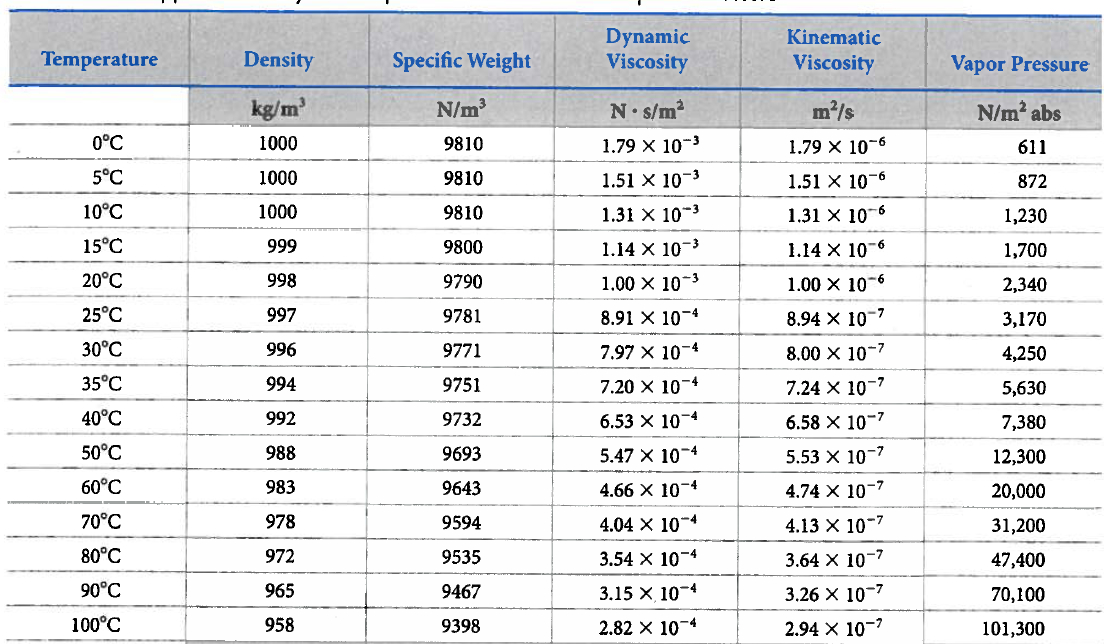
\includegraphics[width=6in]{./2-Algorithms/FluidData.jpg} 
   \caption{Table of water properties in SI units (from CITE)}
   \label{fig:FluidData}
\end{figure}

Now suppose we wished to estimate the density of water at $44^o$ C.  
The two ordered pairs of temperature and density that surround $44^o$ C are $(40^o~C,992~kg/m^3)$ and $(50^o~C,988~kg/m^3)$.
So, to estimate the unknown density we can apply Equation \ref{eqn:InterpolationEquation2} and obtain the following result
\begin{equation}
y^*=992+\frac{(988-992)(44-40)}{(50-40)}=990.4
\label{eqn:DensityInterpolation}
\end{equation}

We might want to do this a lot, so we could write a simplistic script in R and remember to load it into our environment when we need it

\begin{lstlisting}[caption=R code demonstrating the interpolation equation, label=lst:InterpolatePairs]
# EXAMPLE # ** Interpolating Between Tabulated Pairs
interpolate2pairs<-function(xstar,x1,y1,x2,y2){
# apply interpolation equation
#   does not trap errors (divide by zero, etc)
  ystar <- y1 + (y2-y1)*(xstar-x1)/(x2-x1)
  return(ystar)
}
# In R Console
> interpolate2pairs(44,40,992,50,988)
[1] 990.4
> 
\end{lstlisting}   

For a single interrogation of a table we can stop here, but in many instances we have to interrogate a table a lot -- we want some kind of program structure to handle the work so all we have to do is pass the temperature value and have the program return the density.

\subsubsection{Interpolation of Values in Two Arrays}
To accomplish repeated interpolation we will need to have: (1) an interpolating method (we have the beginning of one above in Listing \ref{lst:InterpolatePairs}), (2) the entire table so we don't have to enter the pairs, and (3) a way to  automatically search the table so we don't have to look up values and supply them to the interpolator.

The table itself in this instance is relatively small, so we can simply assign values to some constant arrays in below in Listing \ref{lst:AssignFluidConstants}.

\begin{lstlisting}[caption=R code assigning Liquid Properties, label=lst:AssignFluidConstants]
# EXAMPLE # ** Assigning Constants
tempSI<-c(0.00,5.00,10.00,15.00,20.00,25.00,30.00,35.00,
   40.00,50.00,60.00,70.00,80.00,90.00,100.00)
densitySI<-c(1000.00,1000.00,1000.00,999.00,998.00,997.00,996.00,
   994.00,992.00,988.00,983.00,978.00,972.00,965.00,958.00)

# In R Console
> cbind(tempSI,densitySI)
      tempSI densitySI
 [1,]      0      1000
 [2,]      5      1000
 [3,]     10      1000
 [4,]     15       999
 [5,]     20       998
 [6,]     25       997
 [7,]     30       996
 [8,]     35       994
 [9,]     40       992
[10,]     50       988
[11,]     60       983
[12,]     70       978
[13,]     80       972
[14,]     90       965
[15,]    100       958
> 
\end{lstlisting}  

Returning to our example, the value $44$ lies between \texttt{tempSI[9]} and \texttt{tempSI[10]}, so we desire an algorithm that starts at \texttt{tempSI[1]} and determines if the search value is between \texttt{tempSI[1]} and \texttt{tempSI[2]}, if not, then increment the row counter and determine if the search value is between \texttt{tempSI[2]} and \texttt{tempSI[3]}, and so on.

Once we locate in the searched array where the value lies then the interpolation uses the lower and upper elements of the range to interpolate.  In the case of our example, once we determine the $44$ lies between  \texttt{tempSI[9]} and \texttt{tempSI[10]}, then the interpolation equation is

\begin{equation}
y^*=\texttt{densitySI[9]}+\frac{(\texttt{densitySI[10]}-\texttt{densitySI[9]})(44-\texttt{tempSI[9]})}{(\texttt{tempSI[10]}-\texttt{tempSI[9]})}
\label{eqn:InterpolationArrayEquation}
\end{equation}

Listing \ref{lst:GetAValue} is an \textbf{R} script that implements the search and interpolation just described.  The script assumes that the searched array ($x$) is ordered and increasing -- not a trivial assumption!  The script has some limited error handling to test if the search value actually lies in the total range of the array before beginning the search.  Once these tests are passed, then the code searches in the $x$ array for the search value $x^*$ and finds the two rows that contain the value.  Once the rows are located, the interpolation equation is used.

\begin{lstlisting}[caption=R code to Search and Interpolate, label=lst:GetAValue]
# EXAMPLE # ** Search and Interpolate
  getAvalue <- function(x,xvector,yvector){
    # returns a y value for x interpolated from (xvector,yvector)
    # xvector is assumed to be in a monotonic sequence
    # function performs limited error checks
    # NULL return is error indicator
    # T.G. Cleveland July 2007 
    #
    xvlength <- length(xvector)
    yvlength <- length(yvector)
    # check that vector lengths same
    if(xvlength != yvlength){
      message("vectors xvector and yvector different lengths -- exiting function")
      return()
    }
    # check that x in range xvector
    if(x < min(xvector)){
      message(" x too small -- exiting function")
      return()
    }
    if(x > max(xvector)){
      message(" x too big -- exiting function")
      return()
    }
    #
    for (i in 1:(xvlength-1)){
      if( (x >= xvector[i]) & (x < xvector[i+1]) ){
        result = yvector[i]+(yvector[i+1]-yvector[i])*(x - xvector[i])/
        (xvector[i+1]-xvector[i])
        return(result)
      }
      # next row  
    }
    # check if at endpoint
    if( (x >= xvector[xvlength-1]) & (x <= xvector[xvlength]) ){
      result = yvector[i]+(yvector[i+1]-yvector[i])*(x - xvector[i])/
      (xvector[i+1]-xvector[i])
      return(result)
    }
    # should never get to next line
    message("something is really wrong -- check the vectors!")
    return()
  }
 # In R Console:  
> getAvalue(44,tempSI,densitySI)
[1] 990.4
> 
  \end{lstlisting}  

Now we can load and run the \texttt{getAvalue} script and supply the two vectors plus the search value as shown in Listing \ref{lst:GetAValue}

This look-up process is readily transferred to other cases, we do have to decide if the data will be coded as constants (as was done here) or read from a file -- if the database is large the file read option is best.  In terms of building a generic look-up tool several things actually happen in a particular order.

\begin{enumerate}
\item The function call loads in the table (of reading from a file, we would have to forward declare the vectors).
\item The function searches the first vector for the bounding location of the search variable.
\item Once the boundaries are located, the interpolation is performed -- notice how the last boundary pair is handled.
\end{enumerate}

Now we can combine the data assignment, the search and interpolate into a single function so when we want to evaluate in the future we only need the single function.

Listing \ref{lst:getDensitySI} is an example of everything combined.   Here I have embedded the \texttt{getAvalue} script into the function so the whole function itself is portbable (we don't have keep track of \texttt{getAvalue}).  This embedding can be replaced with a load from a library (but then we must keep track of the path).  

The library way is preferable; if \texttt{getAvalue} needs changing, we will have to change every instance of it in the code, if we miss one the code may still run and it could be years before we discover the error because a single instance of code fragment within a larger code was missed -- its far better to only change a single instance of the function when maintenance is necessary.

\begin{lstlisting}[caption=R code to Return Water Density for Given Temperature, label=lst:getDensitySI]
# Script to return water density in SI units as a function of temperature
getDensitySI<-function(t){
# load the getAvalue() function ###################################################
  getAvalue <- function(x,xvector,yvector){
    # returns a y value for x interpolated from (xvector,yvector)
    # NULL return is error indicator
    #
    xvlength <- length(xvector)
    yvlength <- length(yvector)
    # check that vector lengths same
    if(xvlength != yvlength){
      message("vectors xvector and yvector different lengths -- exiting function")
      return()
    }
    # check that x in range xvector
    if(x < min(xvector)){
      message(" x too small -- exiting function")
      return()
    }
    if(x > max(xvector)){
      message(" x too big -- exiting function")
      return()
    }
    #
    for (i in 1:(xvlength-1)){
      if( (x >= xvector[i]) & (x < xvector[i+1]) ){
        result = yvector[i]+(yvector[i+1]-yvector[i])*(x - xvector[i])/
          (xvector[i+1]-xvector[i])
        return(result)
      }
      # next row  
    }
    # check if at endpoint
    if( (x >= xvector[xvlength-1]) & (x <= xvector[xvlength]) ){
      result = yvector[i]+(yvector[i+1]-yvector[i])*(x - xvector[i])/
        (xvector[i+1]-xvector[i])
      return(result)
    }
    # should never get to next line
    message("something is really wrong -- check the vectors!")
    return()
  }
#########################################################################################
# load the data vectors, tempSI and densitySI
tempSI<-c(0.00,5.00,10.00,15.00,20.00,25.00,30.00,35.00,
  40.00,50.00,60.00,70.00,80.00,90.00,100.00)
densitySI<-c(1000.00,1000.00,1000.00,999.00,998.00,997.00,996.00,
  994.00,992.00,988.00,983.00,978.00,972.00,965.00,958.00)
# now call getAValue
result<-getAvalue(t,tempSI,densitySI)
return(result)
}
  \end{lstlisting}  

The ``library'' approach is demonstrated in Listing \ref{lst:PlotDensity}; in this listing the path in the \texttt{source()} command is unique to my machine -- your path is likely to be different.  I find it is useful to contain all the various codes into a single directory and source that directory once to find the path, then change all the source calls to that path.  In fact that path can be a string variable and the referencing can be automatic (as long as the files exist!).

Once the look-up function is built then we can  interrogate the table many times; and even build a plot of the table -- these features are demonstrated in Listing \ref{lst:PlotDensity}.

\begin{lstlisting}[caption=R code demonstrating use of getDensitySI(), label=lst:PlotDensity]
## In R Console  
> # Example demonstrating use of functions
> # load in the functions (must exist -- use path on your machine)
> source('~/Dropbox/1-CE-TTU-Classes/UnderDevelopment/
   CE4333-PCH-R/6-RScripts/getAvalue.R')
> source('~/Dropbox/1-CE-TTU-Classes/UnderDevelopment/
   CE4333-PCH-R/6-RScripts/getDensitySI.R')
> # Now use them
> getDensitySI(44)
[1] 990.4
> getDensitySI(54)
[1] 986
> getDensitySI(88)
[1] 966.4
> t<-seq(0,100,2) # make a temperature vector 0 to 100 in 2 degree increments
> d<-numeric(0) # forward declare d to store results
> howMany<-length(t)
> for(i in 1:howMany){
+     d[i]<-getDensitySI(t[i])
+ }
> plot(t,d,type="l",xlab="Degrees Celsius",ylab="Density (kg/m^3)")
> 
\end{lstlisting}  

The resulting plot is shown on Figure \ref{fig:PlotDensity} below.
\begin{figure}[htbp] %  figure placement: here, top, bottom, or page
   \centering
   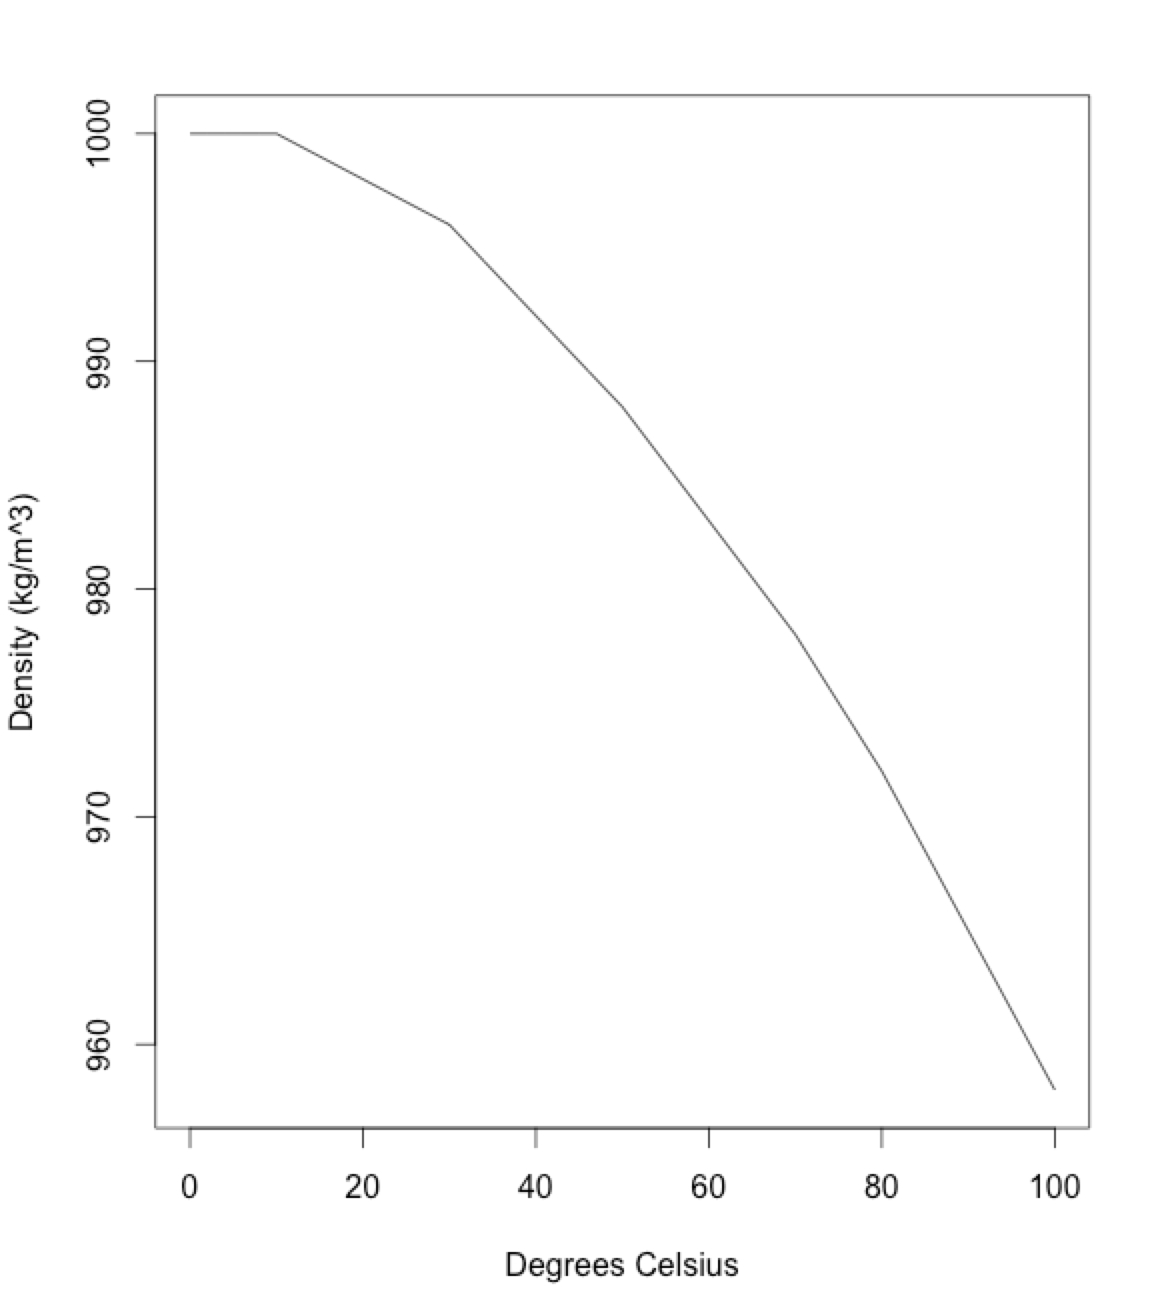
\includegraphics[width=5in]{./2-Algorithms/PlotDensity.jpg} 
   \caption{Plot of density versus temperature generated using the \texttt{getDensity()} function.}
   \label{fig:PlotDensity}
\end{figure}

%%%%%%%%%%%%%%%%%%%% CHAPTER 3 %%%%%%%%%%%%%%%%%%%%%%%%%%
%%%%% Variables and Operators %%%%%%%%%%%%%%%%%%%%%%%%%%%%%%%%%%% 
\subsection{Sorting}
Another frequent task in engineering hydraulics is the seemingly mundane task of sorting or ordering things. 
Here we explore a couple of simple sorting algorithms, just to show some of the thoughts that go into such a task, then will ultimately resort to the internal sorting routines built into R.
\subsubsection{Bubble Sort}
The bubble sort is a place to start despite it's relative slowness.
It is a pretty reviled algorithm (read the Wikipedia entry), but it is the algorithm that a naive programmer might cobble together in a hurry, and despite its shortcomings (its really slow and inefficient), it is robust.

Here is a description of the sorting task as described by \cite{Christian2016} (pg. 65):
\begin{quote}
``Imagine you want to alphabetize your unsorted collection of books. A natural approach would be just to scan across the shelf looking for out-of-order pairs -- Wallace followed by Pynchon, for instance -- and flipping them around. Put Pynchon ahead of Wallace, then continue your scan, looping around to the beginning of the shelf each time you reach the end. When you make a complete pass without finding any more out-of-order pairs on the entire shelf, then you know the job is done.

This process is a Bubble Sort, and it lands us in quadratic time. There are $n$ books out of order, and each scan through the shelf can move each one at most one position. (We spot a tiny problem, make a tiny fix.) So in the worst case, where the shelf is perfectly backward, at least one book will need to be moved n positions. Thus a maximum of $n$ passes through $n$ books, which gives us $O(n2)$ in the worst case.\footnote{Actually, the average running time for Bubble Sort isn't any better, as books will, on average, be $n/2$ positions away from where they?re supposed to end up. One would round the $n/2$ passes of $n$ books up to $O(n2)$.}
$\dots \dots$  For instance, it means that sorting five shelves of books will take not five times as long as sorting a single shelf, but twenty-five times as long.''
\end{quote}

Converting the word description into \textbf{R} is fairly simple.  We will have a vector of $n$ numbers (we use a vector because its easy to step through the different positions), and we will scan through the vector once (and essentially find the smallest thing), and put it into the first position.  Then we scan again from the second position and find the smallest thing remaining, and put it into the second position, and so on until the last scan which should have the remaining largest thing.  If we desire a decreasing order, simply change the sense of the comparison.  

Listing \ref{lst:MyBubbleSort.R} is an \textbf{R} script that implements the algorithm -- in the script the actual sort is treated as a function (we may actually want to use it again someday) which is loaded into the programming environment first, then an array is defined, and sorted.  The program (outside of the sorting algorithm) is really quite simple.  
\begin{itemize}
\item Load the sorting function.
\item Load contents into an array to be sorted.
\item Echo (print) the array (so we can verify the data are loaded as anticipated).
\item Sort the array, put the results back into the array (an in-place sort).
\item Report the results.
\end{itemize}

\begin{lstlisting}[caption=R code demonstrating the naive bubble sort, label=lst:MyBubbleSort.R]
##############################################################
rm(list=ls())  # clear the object list (i.e. deallocate and clear memory)
### Bubble Sort Function -- Needs to be defined before sending array to sort ###
# Bubble Sort Function
# MyLocation: ~/Dropbox/1-CE-TTU-Classes/CE4333-PCH-R/1-Lectures/Lecture03/ScriptsInLecture
# Bubble Sort with array indexing starting at [1] 
# Compare to Python or C where arrays start at [0])
# by: Theodore G. Cleveland 2017-0317
################################################################
bubble <- function(array)
{
  # Prepare the sort, need to know how many things and need a temporary store
  swap <- numeric(0) # temporary store (aka swap location)
  howMany <- length(array) # how many things to be sorted
  # The actual sorting process
  for (irow in 1:(howMany-1))
  {
    for (jrow in 1:(howMany-irow))
    {
      if( array[jrow] > array[jrow+1])
      {
        swap <- array[jrow];
        array[jrow] <- array[jrow+1];
        array[jrow+1] <- swap;
      }
    } 
  }
  # return result (sort in-place)
  return(array)
}
##############################################################

##############################################################
xarray <- c(1003,3.2,55.5,-0.0001,-6,666.6,102)  # the array to sort
print(xarray)
xarray <- bubble(xarray)
print(xarray)
##############################################################
\end{lstlisting}  

Figure \ref{fig:MyBubbleSort.jpg} is a screen capture of the script running.   
In the figure we see that the program (near the bottom of the file) assigns the values to the vector named array and the initial order of the array is $[1003,3.2,55.5,-0.0001,-6,666.6,102]$.   
The smallest value in the example is $-6$ and it appears in the 5-th position, not the 1-st as it should.  

The first pass through the array will move the largest value, $1003$, in sequence to the right until it occupies the last position.
Repeated passes through the array move the remaining largest values to the right until the array is ordered.  
One can consider the values of the array at each scan of the array as a series of transformations (\texttt{irow}-th scan) -- in practical cases we don't necessarily care about the intermediate values, but here because the size is manageable and we are trying to get our feet wet with algorithms, we can look at the values.

The sequence of results (transformations) after each pass through the array is shown in the following list:
\begin{enumerate}
\item Initial value: $[1003,3.2,55.5,-0.0001,-6,666.6,102]$.
\item First pass: $[3.2,55.5,-0.0001,-6,666.6,102,1003]$.
\item Second pass: $[3.2,-0.0001,-6,55.5,102,666.6,1003]$.
\item Third pass: $[-0.0001,-6,3.2,55.5,102,666.6,1003]$.
\item Fourth pass: $[-6,-0.0001,3.2,55.5,102,666.6,1003]$.
\item Fifth pass:  $[-6,-0.0001,3.2,55.5,102,666.6,1003]$. Sorted, fast scan.
\item Sixth pass: $[-6,-0.0001,3.2, 55.5,102,666.6,1003]$.  Sorted, fast scan.
\end{enumerate}
\begin{figure}[h!] %  figure placement: here, top, bottom, or page
   \centering
   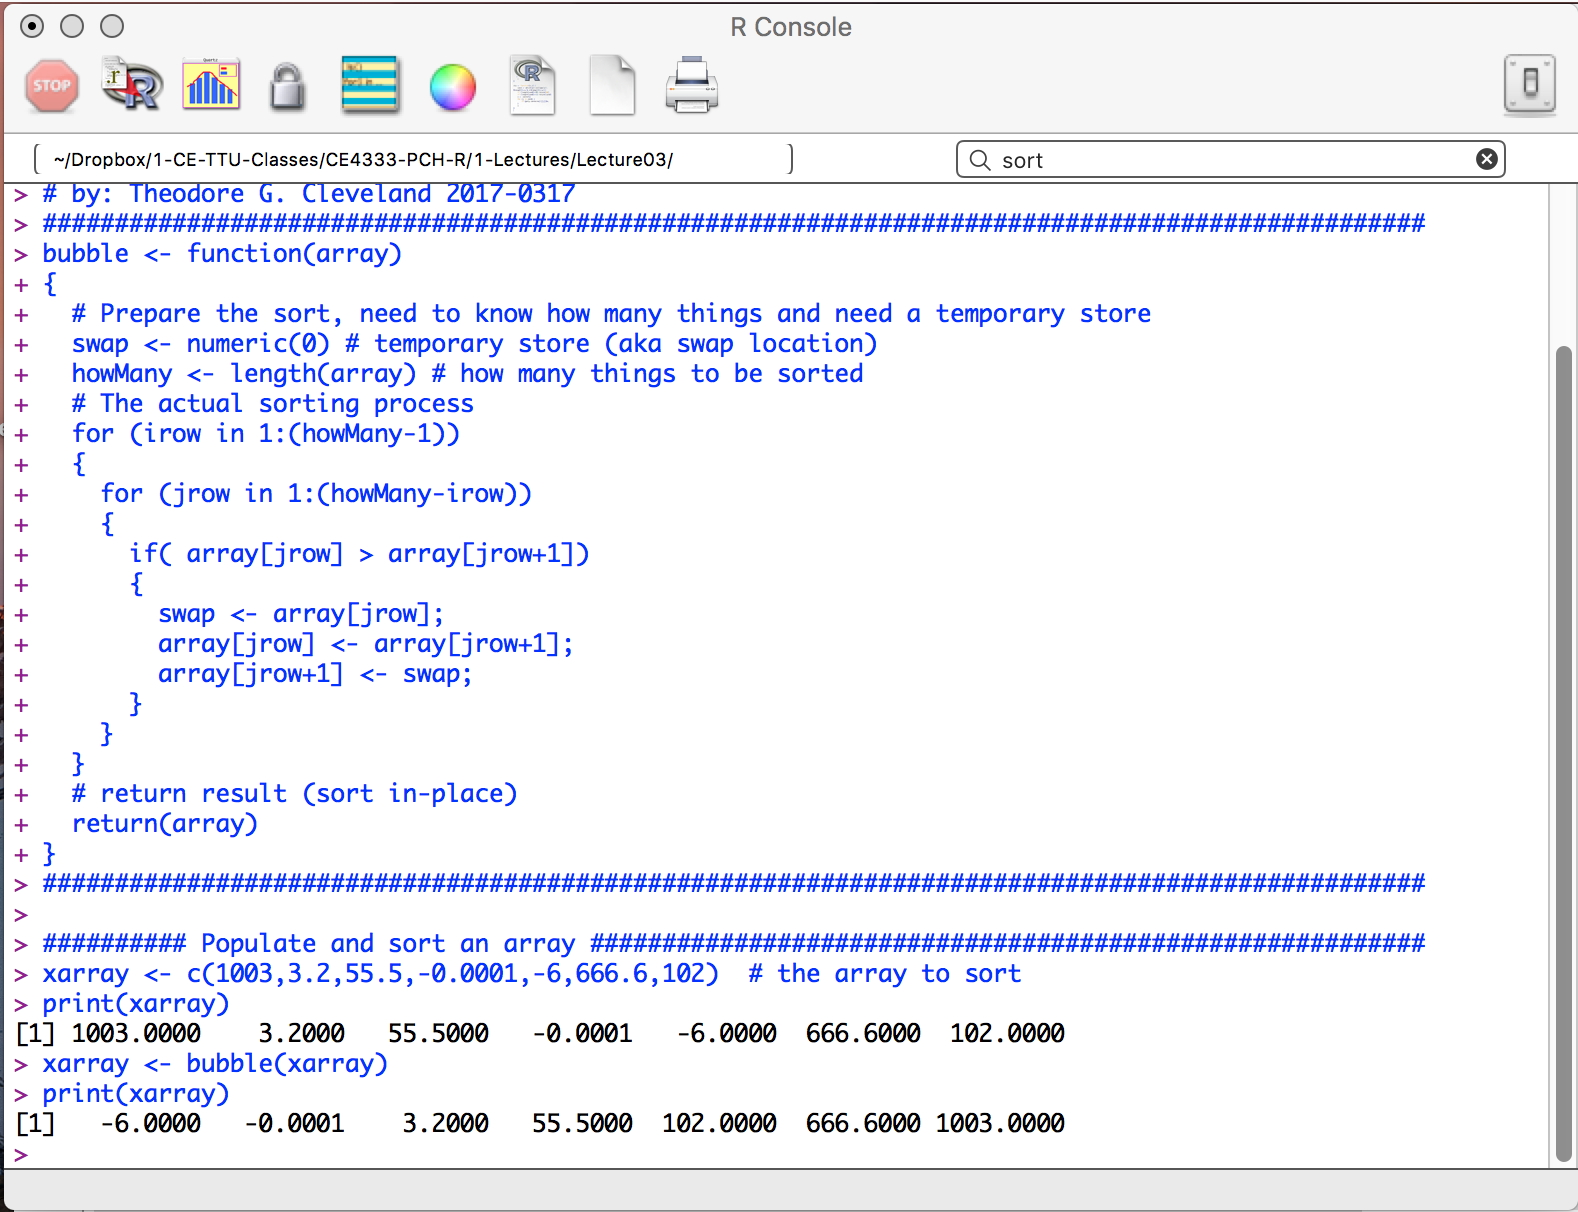
\includegraphics[width=6in]{./2-Algorithms/MyBubbleSort.jpg} 
   \caption{Bubble Sort implemented in \textbf{R}}
   \label{fig:MyBubbleSort.jpg}
\end{figure}

We could probably add additional code to break from the scans when we have a single pass with no exchanges -- while meaningless in this example, for larger collections of things, being able to break out when the sorting is complete is a nice feature.
\clearpage

\subsubsection{Insertion Sort}
The next type of sorting would be to select one item and locate it either left or right of an adjacent item based on its size -- like sorting a deck of cards, or perhaps a better description -- again using the bookshelf analog from \cite{Christian2016} (pg. 65):
\begin{quote}
``$\dots \dots$ You might take a different tack -- pulling all the books off the shelf and putting them back in place one by one. You'd put the first book in the middle of the shelf, then take the second and compare it to the first, inserting it either to the right or to the left. Picking up the third book, you'd run through the books on the shelf from left to right until you found the right spot to tuck it in. Repeating this process, gradually all of the books would end up sorted on the shelf and you'd be done. Computer scientists call this, appropriately enough, Insertion Sort. The good news is that it's arguably even more intuitive than Bubble Sort and doesn't have quite the bad reputation. The bad news is that it's not actually that much faster. You still have to do one insertion for each book. And each insertion still involves moving past about half the books on the shelf, on average, to find the correct place.

Although in practice Insertion Sort does run a bit faster than Bubble Sort, again we land squarely, if you will, in quadratic time. Sorting anything more than a single bookshelf is still an unwieldy prospect.''
\end{quote}

Listing \ref{lst:MyInsertionSort.R} is an \textbf{R} implementation of a straight insertion sort.  
The script is quite compact, and I used indentation and extra line spacing to keep track of the scoping delimiters.
The sort works as follows, take the an element of the array (start with 2 and work to the right) and put it into a temporary location (called \texttt{swap} in my script).  Then compare locations to the left of \texttt{swap}.  If smaller, then break from the loop, exchange values, otherwise the values are currently ordered. Repeat (starting at the next element) , when all elements have been traversed the resulting vector is sorted.  Here are the transformations for each pass through the outer loop:
\begin{enumerate}
\item Pass 0: $[1003,3.2,55.5,-0.0001,-6,666.6,102]$, Initial array.
\item Pass 1: $[3.2,1003,55.5,-0.0001,-6.,666.6,102]$.
\item Pass 2: $[3.2,55.5,1003,-0.0001,-6.,666.6,102]$.
\item Pass 3: $[-0.0001,3.2,55.5,1003,-6.,666.6,102]$.
\item Pass 4: $[-6,-0.0001,3.2,55.5,1003.,666.6,102]$.
\item Pass 5: $[-6,-0.0001,3.2,55.5,666.6,1003,102]$.
\item Pass 6: $[-6,-0.0001,3.2,55.5,102,666.6,1003]$, Sorted array.
\end{enumerate}
Figure \ref{fig:MyInsertionSort.jpg} is a screen capture of the insertion sort in operation.  
Insertion sorting is reasonably fast for small lists (about 50 or so elements) and forms the basis of the internal sorts in other routines that divide up the overall list into smaller lists, sort the smaller lists, then uses a merge to collate back to the overall list (now sorted).
\begin{lstlisting}[caption=R code demonstrating the insertion sort, label=lst:MyInsertionSort.R]
### Straight Insertion Sort Function by: Theodore G. Cleveland 2017-0317
rm(list=ls())  # clear the object list (i.e. deallocate and clear memory)
################################################################
insertSort <- function(array){
# Prepare the sort, need to know how many things and need a temporary store
  swap <- numeric(0) # temporary store (aka swap location)
  howMany <- length(array) # how many things to be sorted
  for (j in 2:howMany)  # select each position in turn
    {
    test <- 0           # set a test value, used to insert later
    swap <- array[j]    # current position to swap
    for (i in seq(j-1,1,by=-1)) #find place to insert by ...
      {
      if (array[i] <= swap)  # test if current position is bigger
        {
        test <- 1            # if true set test to 1, break inner loop
        break
        }
      array[i+1] <- array[i]  # otherwise exchange postions
      }
    if(test == 1)             # if broke from loop, insert swap
      array[i+1] <- swap      
    else
      i = 0
      array[i+1] <- swap      # otherwise swap goes to first position
    }
  return(array) }    # return result (sort in-place)
##############################################################
xarray <- c(1003,3.2,55.5,-0.0001,-6,666.6,102)  # the array to sort
print(xarray)
xarray <- insertSort(xarray)
print(xarray)
##############################################################
\end{lstlisting}  


\begin{figure}[h!] %  figure placement: here, top, bottom, or page
   \centering
   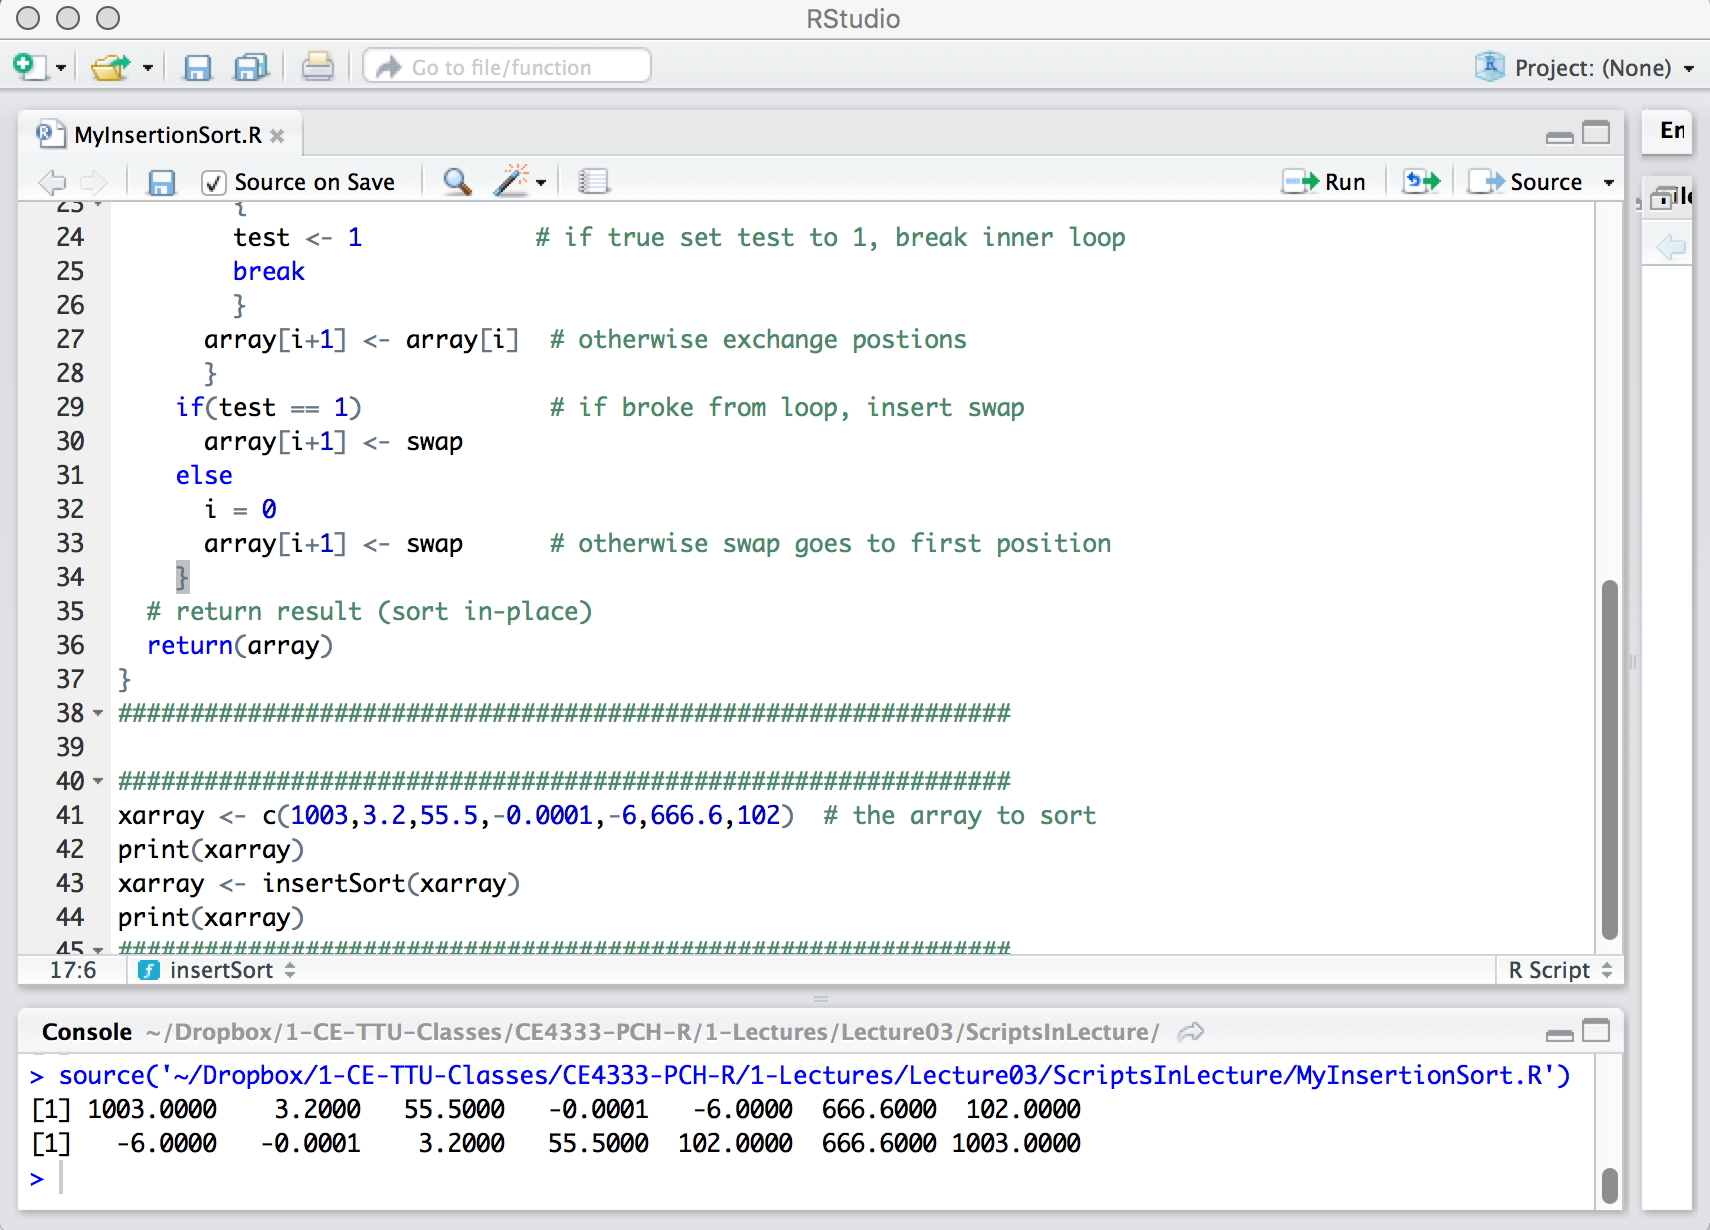
\includegraphics[height=4.2in]{./2-Algorithms/MyInsertionSort.jpg} 
   \caption{Insertion Sort implemented in \textbf{R}}
   \label{fig:MyInsertionSort.jpg}
\end{figure}

\subsubsection{Merge Sort}
A practical extension of these slow sorts is called the Merge Sort.  It is an incredibly useful method.  One simply breaks up the items into smaller arrays, sorts those arrays - then merges the sub-arrays into larger arrays (now already sorted), and finally merges the last two arrays into the final, single, sorted array.

Here is a better description, again from \cite{Christian2016}:
\begin{quote}
``$\dots \dots$ information processing began in the US censuses of the nineteenth century, with the development, by Herman Hollerith and later by IBM, of physical punch-card sorting devices. In 1936, IBM began producing a line of machines called ``collators'' that could merge two separately \textbf{ordered} stacks of cards into one. \textit{As long as the two stacks were themselves sorted}, the procedure of merging them into a single sorted stack was incredibly straightforward and took linear time: simply compare the two top cards to each other, move the smaller of them to the new stack you're creating, and repeat until finished.

The program that John von Neumann wrote in 1945 to demonstrate the power of the stored-program computer took the idea of collating to its beautiful and ultimate conclusion. Sorting two cards is simple: just put the smaller one on top. And given a pair of two-card stacks, both of them sorted, you can easily collate them into an ordered stack of four. Repeating this trick a few times, you'd build bigger and bigger stacks, each one of them already sorted. Soon enough, you could collate yourself a perfectly sorted full deck -- with a final climactic merge, like a riffle shuffle's order-creating twin, producing the desired result. This approach is known today as Merge Sort, one of the legendary algorithms in computer science.''
\end{quote}

There are several other variants related to Merge Sort; Quicksort and Heapsort being relatives.  The creation of a Merge Sort is left to the reader if there is a need, and at this point we can just use the built-in \texttt{sort()}  and/or \texttt{order()} functions in \textbf{R} -- which implements either a Shellsort (useful if character strings are to be sorted) or Quicksort (used if numeric values are supplied).   We also have to supply if we want increasing or decreasing sorts.

\subsubsection{Built-In \textbf{R} Sorts}

Figure \ref{fig:BuiltInRSorts.jpg} illustrates using the built-in functions.  
For an ordinary sort, we simply use the function name \texttt{sort()} and direct its output into an object (it can even be the same vector as shown in the figure). 

If we wish to sort several related columns, based on values in one of the columns, it is easiest to construct a data frame (like a matrix), then order the contents based on one of the columns, and send the results to another data frame, or we can send the result back to itself.  Usually when we are manipulating multiple columns, we are operating in a ``relational database'' kind of mindset, and it is probably to our benefit to not destroy the original association structure.  Be aware of the syntax of a dataframe function, you will notice there is a comma that appears at the end of the function that is important for the script to function.

For example, \texttt{z <- z[order(xarray),]} will function as shown, \\ whereas \texttt{zztop <- z[order(xarray)]} will not.

\begin{figure}[h!] %  figure placement: here, top, bottom, or page
   \centering
   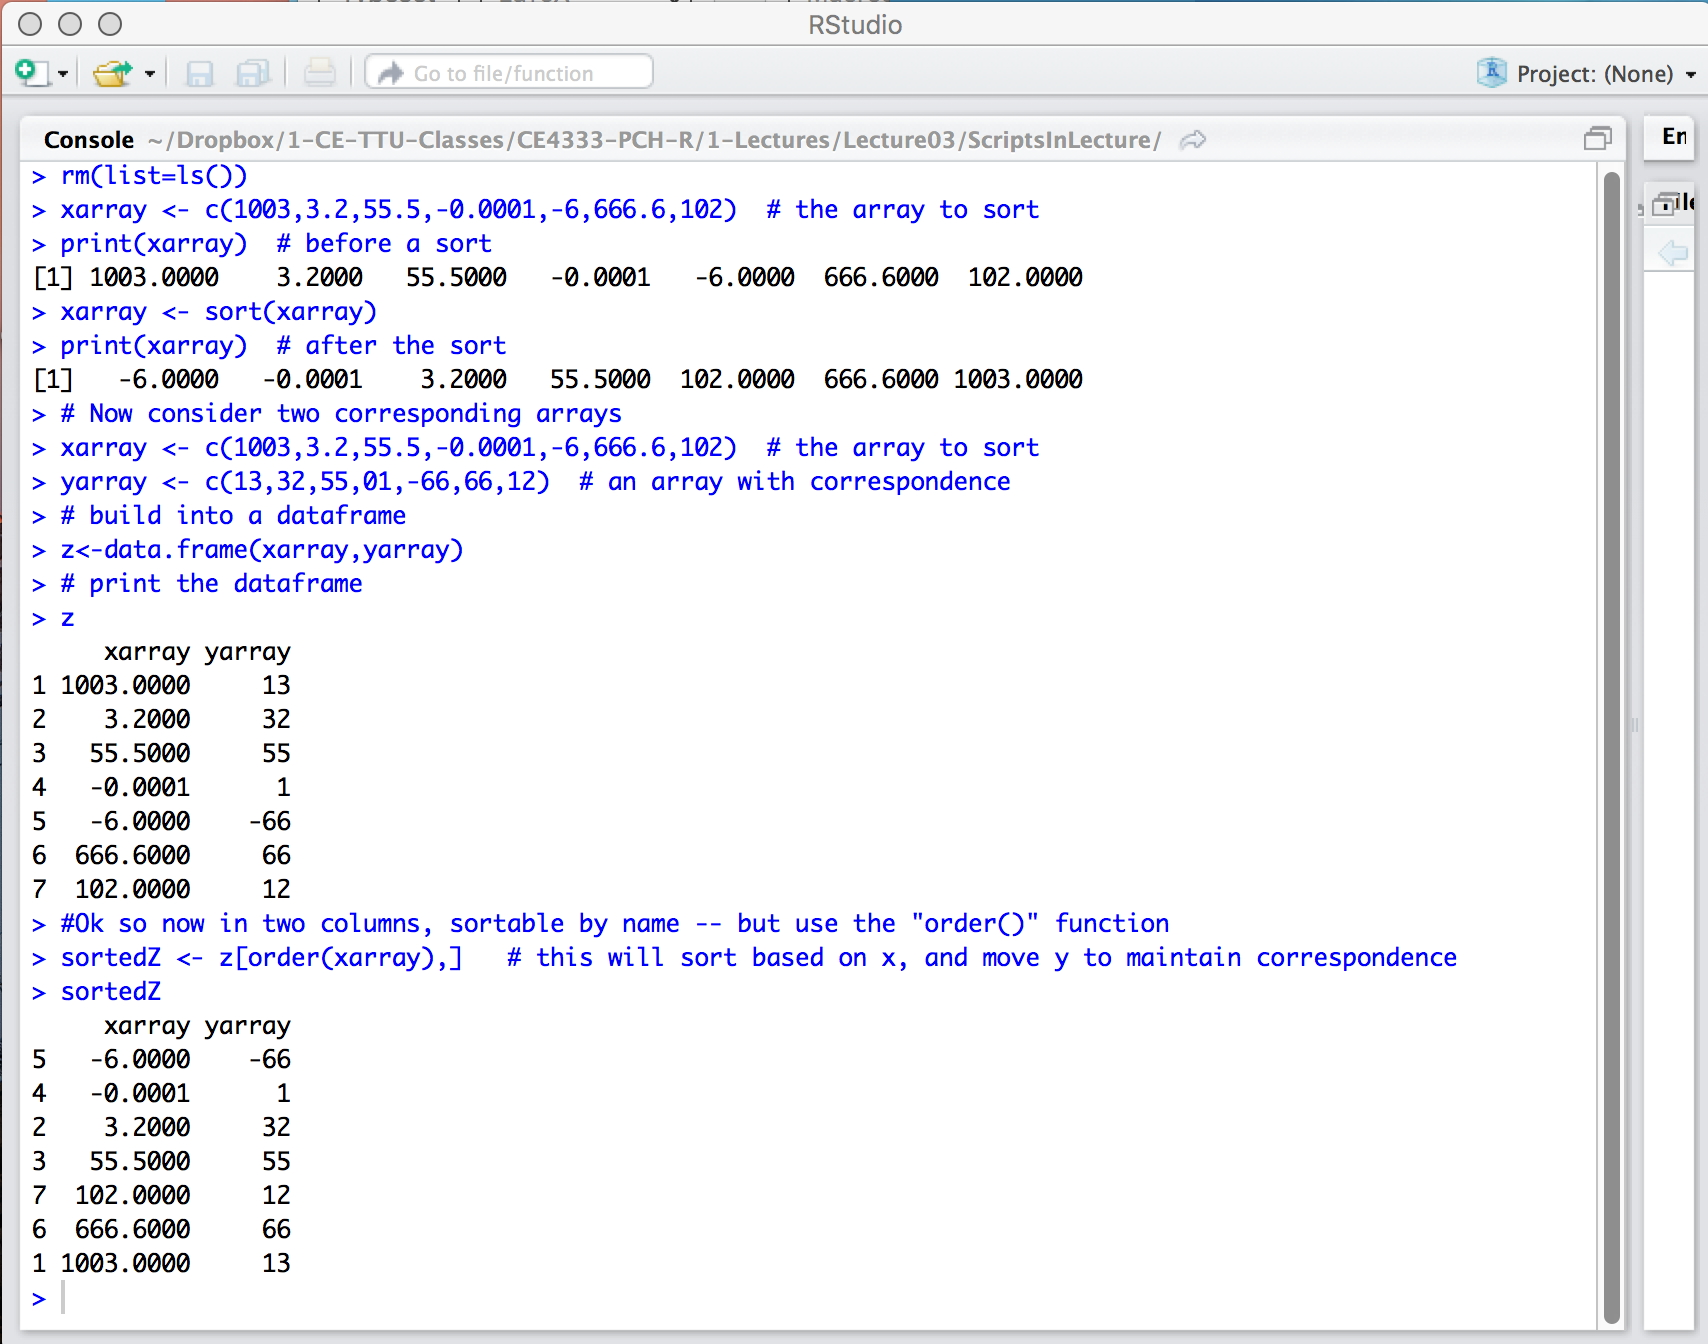
\includegraphics[width=6in]{./2-Algorithms/BuiltInRSorts.jpg} 
   \caption{Sorting using built-in \textbf{R} functions}
   \label{fig:BuiltInRSorts.jpg}
\end{figure}

Now if we return to the interpolation chapter just before this one, we can immediately see a need for sorting.  The interpolation algorithm \textit{assumes} that the explanatory structure (x-axis) is ordered, otherwise the interpolation equation will return garbage.


I conclude the section on sorting with one more quoted section from \cite{Christian2016} about the value for sorting -- which is already relevant to a lot of computational hydraulics:
\begin{quote}
``The poster child for the advantages of sorting would be an Internet search engine like Google. It seems staggering to think that Google can take the search phrase you typed in and scour the entire Internet for it in less than half a second. Well, it can't -- but it doesn't need to. If you're Google, you are almost certain that (a) your data will be searched, (b) it will be searched not just once but repeatedly, and (c) the time needed to sort is somehow ``less valuable'' than the time needed to search. (Here, sorting is done by machines ahead of time, before the results are needed, and searching is done by users for whom time is of the essence.) All of these factors point in favor of tremendous up-front sorting, which is indeed what Google and its fellow search engines do.''
\end{quote}




%%%%%%%%%%%%%%%%%%%%%%%%%%%%%%%%%%%%%%%%%%%%%%%%%%%%

\subsection*{Exercise Set 1}
\begin{enumerate}
\item Build a function \texttt{getDensityUS()} that searches the table in Figure \ref{fig:FluidData} and returns the density of water in US customary units for a value of temperature supplied in degrees Farenheight. \\~\\
Submit your code and screen captures of the density for temperatures of $43^o~F$, $146^o~F$, and $210^o~F$.

\item Later in the class we will need functions to return viscosity to compute head losses in pipe networks.  \\
Build and test a function \texttt{getKinViscosityUS()} that searches the table in Figure \ref{fig:FluidDataUS} and returns the kinematic viscosity of water in US customary units for a value of temperature supplied in degrees Farenheight\\~\\
Submit the code and screen captures of the kinematic viscosity for temperatures of $43^o~F$, $146^o~F$, and $210^o~F$. 

\item Build and test a function \texttt{getKinViscositySI()} that searches the table in Figure \ref{fig:FluidData} and returns the kinematic viscosity of water in SI units for a value of temperature supplied in degrees Celsius \\~\\
Submit the code and screen captures of the kinematic viscosity for temperatures of $13^o~C$, $66^o~C$, and $97^o~C$.

\item Imagine you have two arrays, \texttt{array1} and \texttt{array2} that are linked in the sense that each element of \texttt{array1} is associated with the corresponding element of \texttt{array2}.  You wish to sort based on contents of \texttt{array1} and maintain the correspondence of \texttt{array2}.  In words we would simply modify the script to move and element of \texttt{array2} whenever you move an element of \texttt{array1}.

Modify the Insertion Sort script to accept two arrays, the sort is based on contents of the first array and you are to maintain correspondence with the second array.

Test your script on the following arrays:\\
\texttt{array1} = $[5,6,8,2,3,4,1]$\\
\texttt{array2} = $[24,35,63,3,8,15,0]$\\

when these are reordered, the result should be: \\
\texttt{array1} = $[1,2,3,4,5,6,8]$\\
\texttt{array2} = $[0,3,8,15,35,63]$\\

Then modify your script to read input from an ASCII file that contains the two arrays as columns (like in a spreadsheet) where you will sort on the first column, and carry along the correspondence with the second column.

Apply the script on the file \texttt{es3-pr1.txt}.

\item Repeat the exercise above but use built-in \textbf{R} functions.\footnote{My solution uses the \texttt{data.frame()} and \texttt{order()} functions.  There are probably several other ways to accomplish the goal -- corresponding sorts are hugely important in many practical situations.} 
\end{enumerate}

This exercise set is also located on the class server as \texttt{ES-1}.
%%%%%%%%%%%%%%%%%%%%%%%%%%%%%%%%%%%%%%%%%%%%%%%%%%%%%%%%%%%%%%%
% need more here

%%%%%%%%%%%%%%%%%%%%%%%%%%%%%%%%%%%%%%%%
%\section{Numerical Methods -- Integrals, Derivatives, and Newton's Method}
\subsection{Numerical Integration of Functions}
Numerical integration is the numerical approximation of
\begin{equation}
I = \int_a^b f(x)dx
\end{equation}
 
Consider the problem of determining the shaded area under the curve $y = f(x)$ from $x = a$ to $x = b$, as depicted in Figure \ref{fig:IntegrationPanels}, and suppose that analytical integration is not feasible. 
 
\begin{figure}[h!] %  figure placement: here, top, bottom, or page
   \centering
   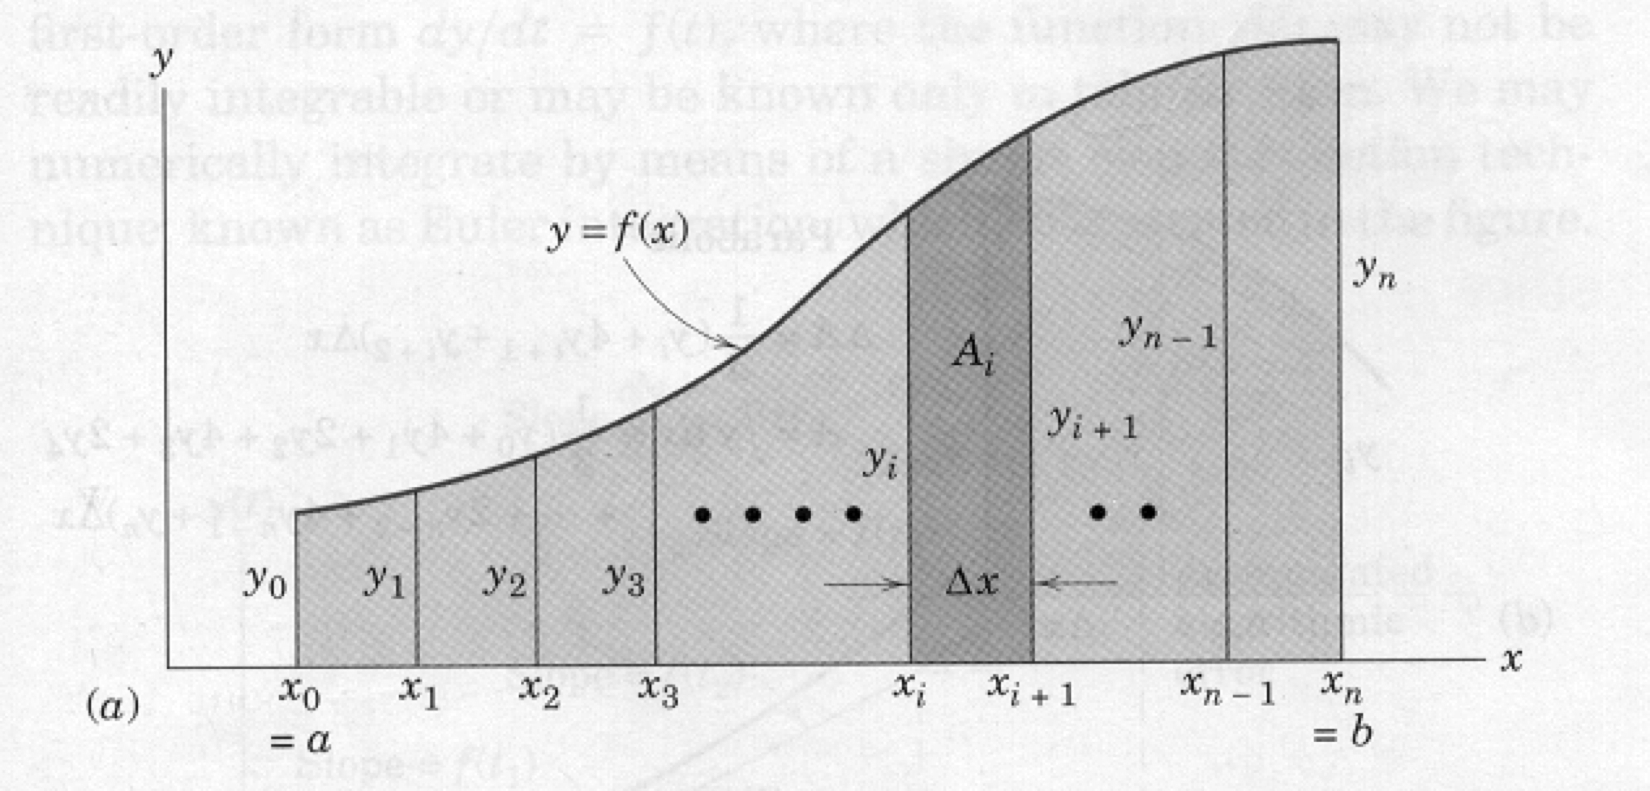
\includegraphics[width=5in]{./3-Differentation/IntegrationPanels.jpg} 
   \caption{Schematic of Panels for Numerical Integration. }
   \label{fig:IntegrationPanels}
\end{figure}

The function may be known in tabular form from experimental measurements or it may be known in an analytical form. 
The function is taken to be continuous within the interval $a < x < b$. 
We may divide the area into $n$ vertical panels, each of width $\Delta x = (b - a)/n$, and then add the areas of all strips to obtain  $A~\approx \int ydx$.

A representative panel of area $A_i$ is shown with darker shading in the figure. 
Three useful numerical approximations are listed in the following sections.    
The approximations differ in how the function is represented by the panels --- in all cases the function is approximated by known polynomial models between the panel end points.

In each case the greater the number of strips, and correspondingly smaller value of $\Delta x$, the more accurate the approximation. 
Typically, one can begin with a relatively small number of panels and increase the number until the resulting area approximation stops changing.

\subsubsection{Rectangular Panels}
Figure \ref{fig:RectangularPanels} is a schematic of a rectangular panels.  The figure is assuming the function structure is known and can be evaluated at an arbitrary location in the $\Delta x$ dimension.  
\begin{figure}[h!] %  figure placement: here, top, bottom, or page
   \centering
   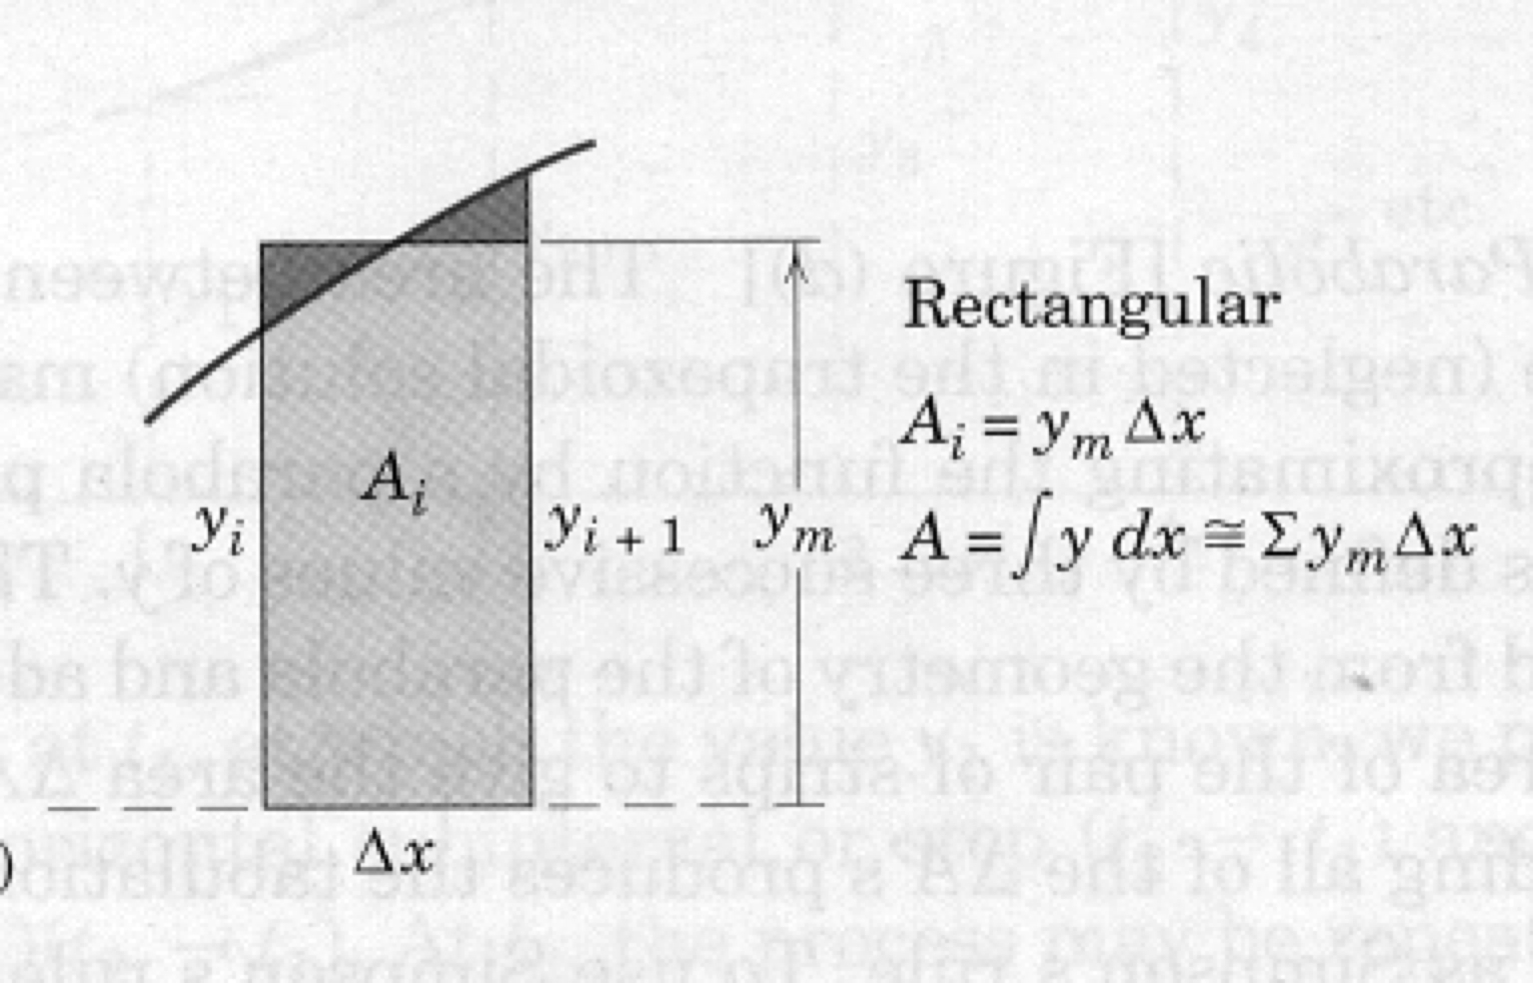
\includegraphics[width=5in]{./3-Differentation/RectangularPanels.jpg} 
   \caption{Rectangular Panel Schematic.}
   \label{fig:RectangularPanels}
\end{figure}
Each panels is treated as a rectangle, as shown by the representative panel whose height $y_m$ is chosen visually so that the small cross-hatched areas are as nearly equal as possible. Thus, we form the sum $\sum y_m$ of the effective heights and multiply by $\Delta x$. For a function known in analytical form, a value for $y_m$ equal to that of the function at the midpoint $x_i + \Delta x /2$ may be calculated and used in the summation.

For tabulated functions, we have to choose to either take $y_m$ as the value at the left endpoint or right endpoint.    This limitation is often quite handy when we are trying to integrate a function that is integrable, but undefined on one endpoint.

Lets try some examples in \textbf{R}.\\

\newpage \textbf{Problem:} Find the area under the curve $y= x\sqrt{1+x^2}$  from $x = 0$ to $x = 2$.

\textbf{Solution:} One solution is shown in Figure \ref{fig:RectExample},which is a screen capture of a rudimentary code that implements the rectangular panel method.\footnote{The exact solution is A=3.393477}   
\begin{figure}[h!] %  figure placement: here, top, bottom, or page
   \centering
   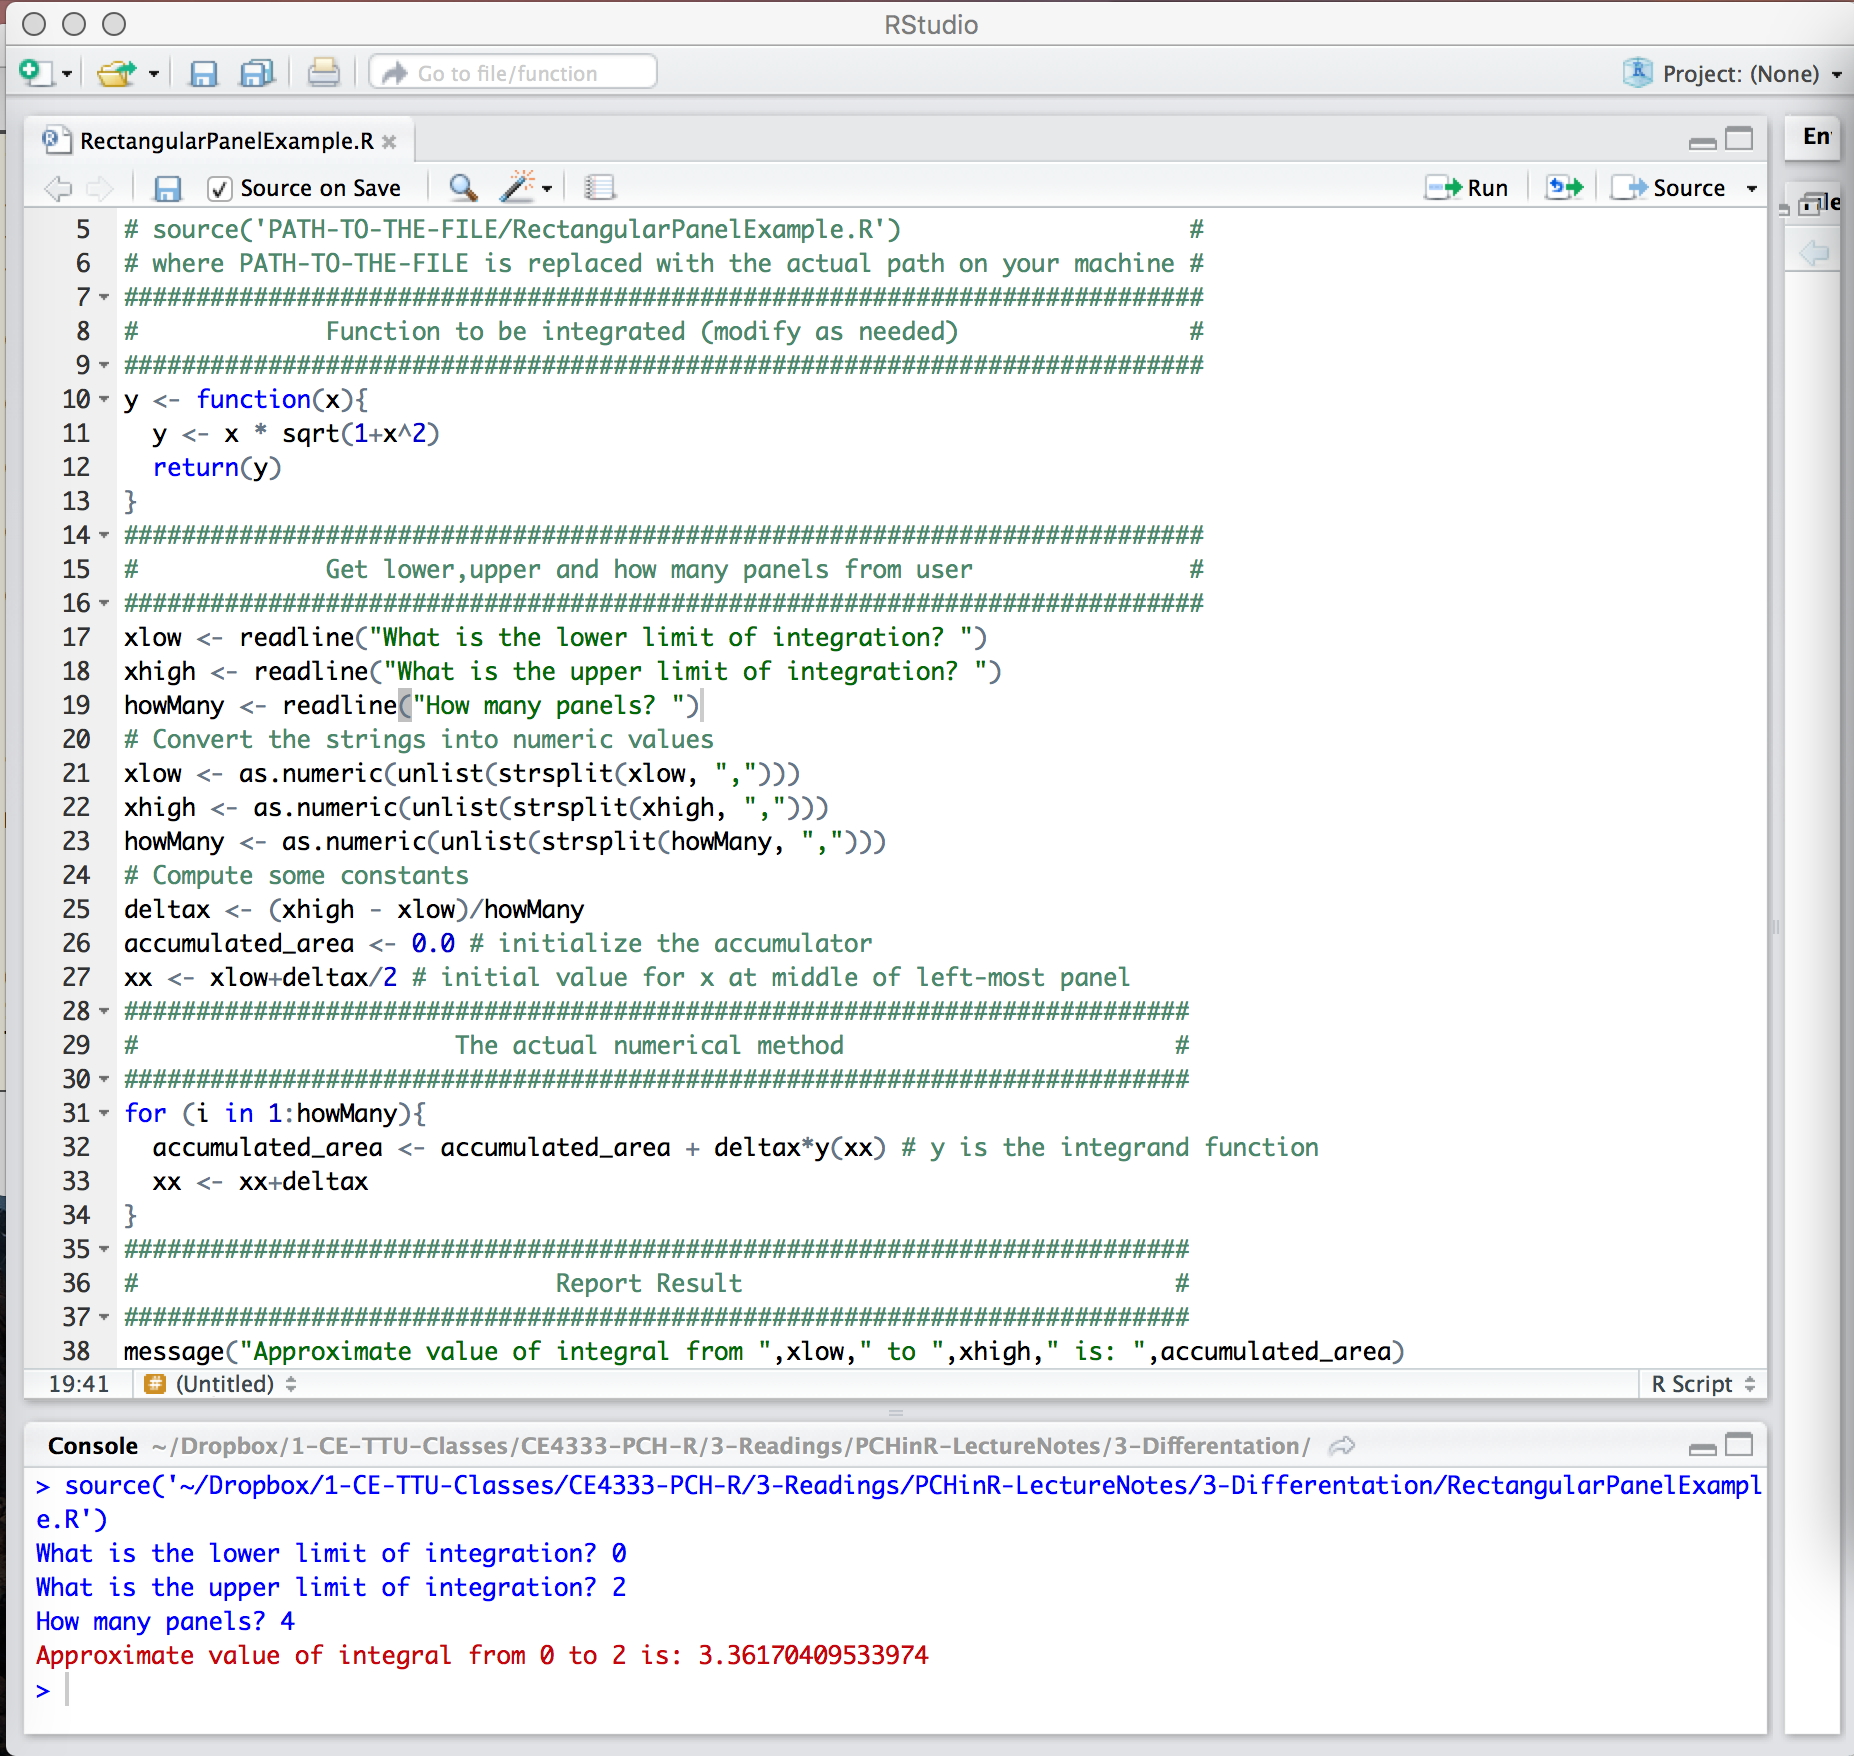
\includegraphics[width=6in]{./3-Differentation/RectExample.jpg} 
   \caption{Rectangular panel example showing code and resulting computed area using just 4 panels.}
   \label{fig:RectExample}
\end{figure}

The script does not implement any kind of error checking -- we could enter text values for the lower and upper values of $x$ as well as the number of panels to use, and the script would attempt to run. 
A better version would force us to enter numeric values, and check for undefined ranges and such; devotion to error trapping is typical for professional programs where you are going to distribute executable modules and not expect the end user to be a programmer.

For the time being, we will accept this approach (error trapping is left as an exercise), however in your own scripts you should implement error traps where possible -- you may start without them but as you maintain your scripts, you will learn where data entry errors occur and trap them.\footnote{For example, traps are used to force the user to enter a value that actually is meaningful, or select a default value, or internally prevent division by zero.}

The actual listing depicted in Figure \ref{fig:RectExample} is shown in Listing \ref{lst:RectPanels}

\begin{lstlisting}[caption=R code demonstrating Rectangular Panel Numerical Integration, label=lst:RectPanels]
# R script to implement rectangular panel numerical integration
################################# NOTE ####################################
## The interactive input requires the script to be sourced                #
# In R console the command line would be                                  #
# source('PATH-TO-THE-FILE/RectangularPanelExample.R')                    #
# where PATH-TO-THE-FILE is replaced with the actual path on your machine #
###########################################################################
#             Function to be integrated (modify as needed)                #
###########################################################################
y <- function(x){
  y <- x * sqrt(1+x^2)
  return(y)
}
###########################################################################
#             Get lower,upper and how many panels from user               #
###########################################################################
xlow <- readline("What is the lower limit of integration? ")  
xhigh <- readline("What is the upper limit of integration? ")
howMany <- readline("How many panels? ")
# Convert the strings into numeric values
xlow <- as.numeric(unlist(strsplit(xlow, ",")))
xhigh <- as.numeric(unlist(strsplit(xhigh, ",")))
howMany <- as.numeric(unlist(strsplit(howMany, ",")))
# Compute some constants
deltax <- (xhigh - xlow)/howMany  
accumulated_area <- 0.0 # initialize the accumulator
xx <- xlow+deltax/2 # initial value for x at middle of left-most panel
##########################################################################
#                      The actual numerical method                       #
##########################################################################
for (i in 1:howMany){
  accumulated_area <- accumulated_area + deltax*y(xx) # y is the integrand function
  xx <- xx+deltax
}
##########################################################################
#                             Report Result                              #
##########################################################################
message("Approximate value of integral from ",xlow," to ",xhigh," is: ",accumulated_area)
\end{lstlisting}

\begin{figure}[h!] %  figure placement: here, top, bottom, or page
   \centering
   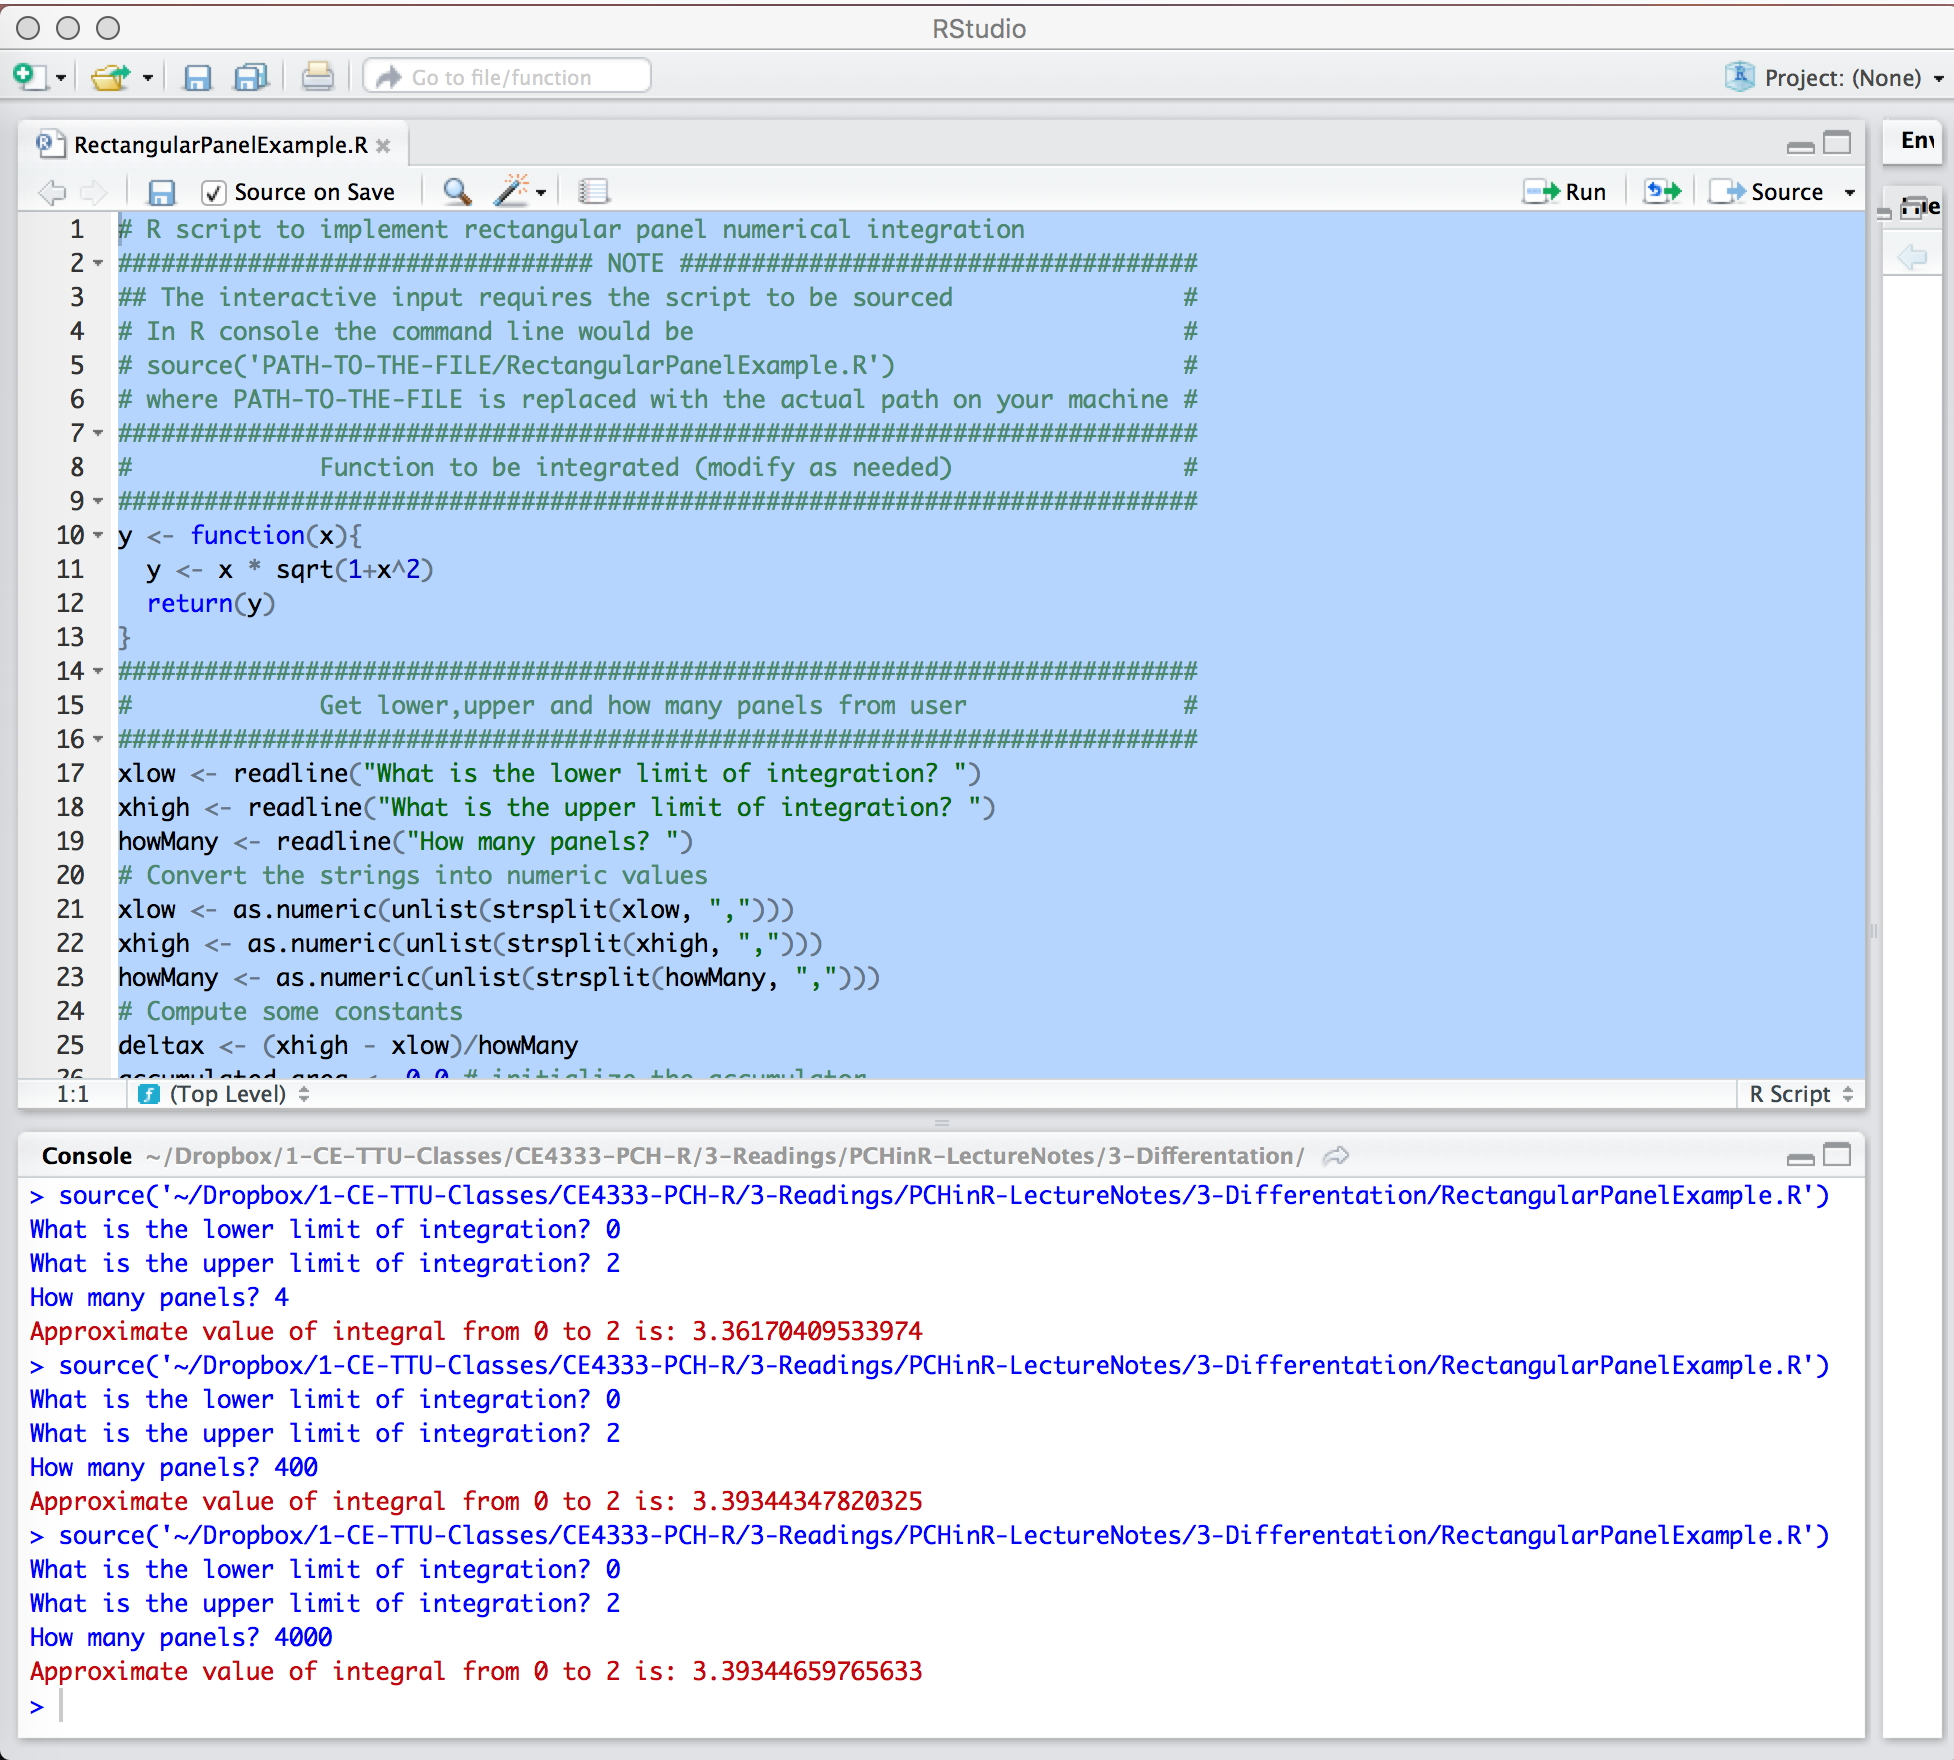
\includegraphics[width=6in]{./3-Differentation/RectExample44.jpg} 
   \caption{Rectangular panel example showing difference in computed area using 4, 400, and 4000 panels.  The 4000 panel result is essentially equivalent to the exact solution.  Such convergence to exact values is typical}
   \label{fig:RectExample44}
\end{figure}
Figure \ref{fig:RectExample44} is the same program run using 4,400, and 4000 panels observe the difference in computed area as well as the results closeness to the exact solution.

\subsubsection{Trapezoidal Panels}
The trapezoidal panels are approximated as shown in Figure \ref{fig:TrapPanels}. The area $A_i$ is the average height $(y_i + y_{i+1} )/2$ times $\Delta x$. Adding the areas gives the area approximation as tabulated.   For the example with the curvature shown, the approximation will be on the low side. For the reverse curvature, the approximation will be on the high side.  The trapezoidal approximation is commonly used with tabulated values.

\begin{figure}[h!] %  figure placement: here, top, bottom, or page
   \centering
   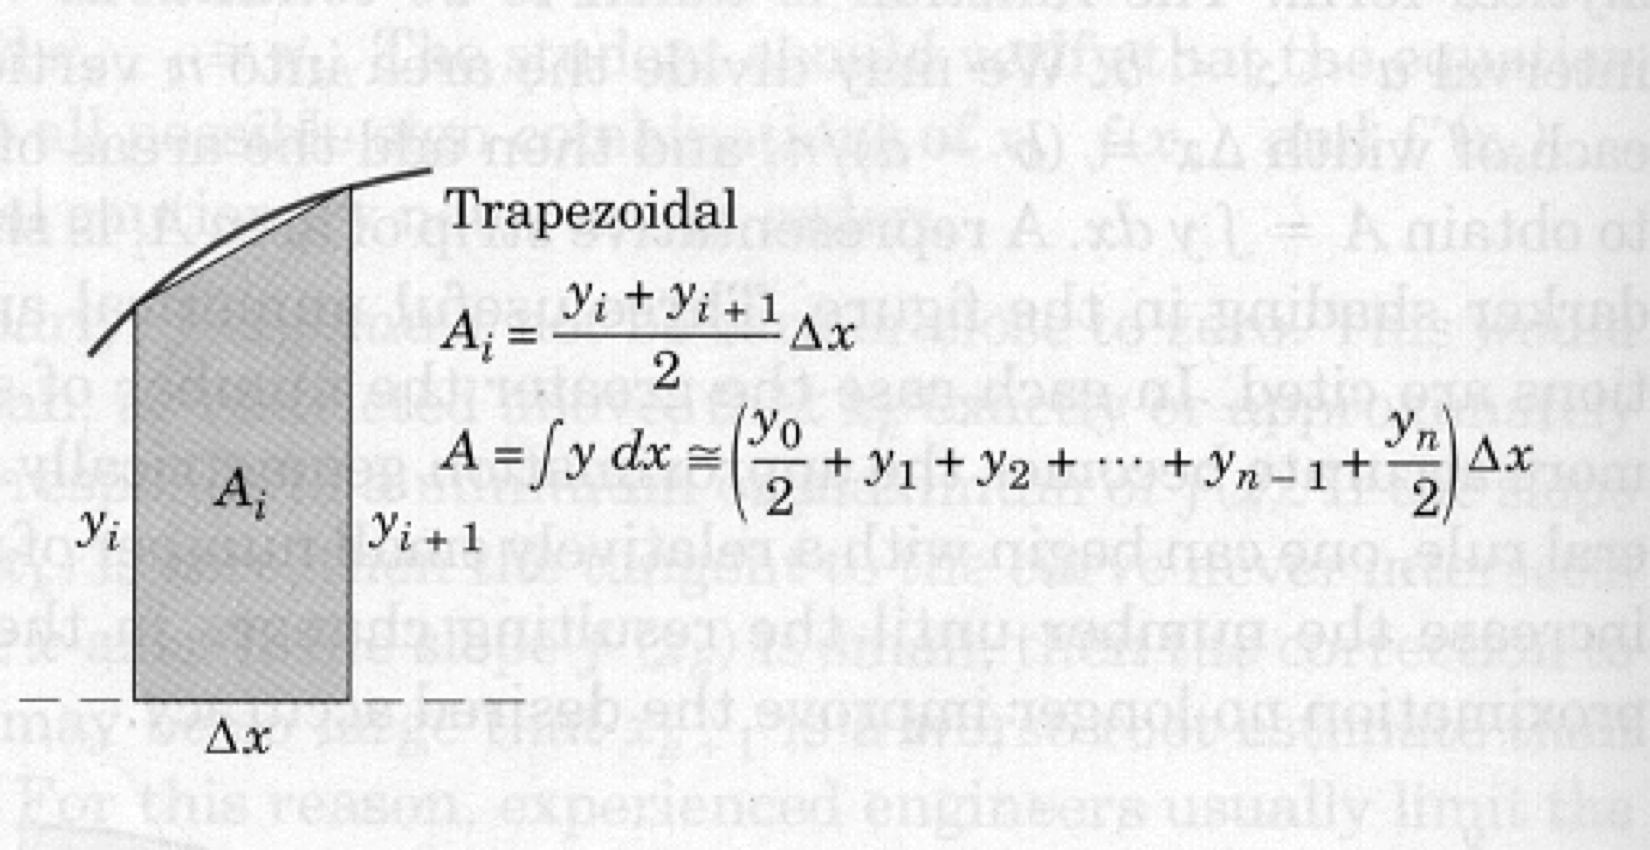
\includegraphics[width=4.3in]{./3-Differentation/TrapPanels.jpg} 
   \caption{Trapezoidal Panel Schematic.}
   \label{fig:TrapPanels}
\end{figure}

The same example as presented for rectangular panels is repeated, except using trapezoidal panels.  The code is changed because we will evaluate at each end of the panel (so no fussing to find an intermediate estimate for where to evaluate the function).

Figure \ref{fig:TrapExample} illustrates the trapezoidal method for approximating an integral.   In the example, the left and right panel endpoints in $x$ are set as separate variables $x_{left}$ and $x_{right}$ and incremented by $\Delta x$ as we step through the count-controlled repetition to accumulate the area.  The corresponding $y$ values are computed within the loop and averaged, then multiplied by $\Delta x$ and added to the accumulator.  Finally the $x$ values are incremented.
 
\begin{figure}[h!] %  figure placement: here, top, bottom, or page
   \centering
   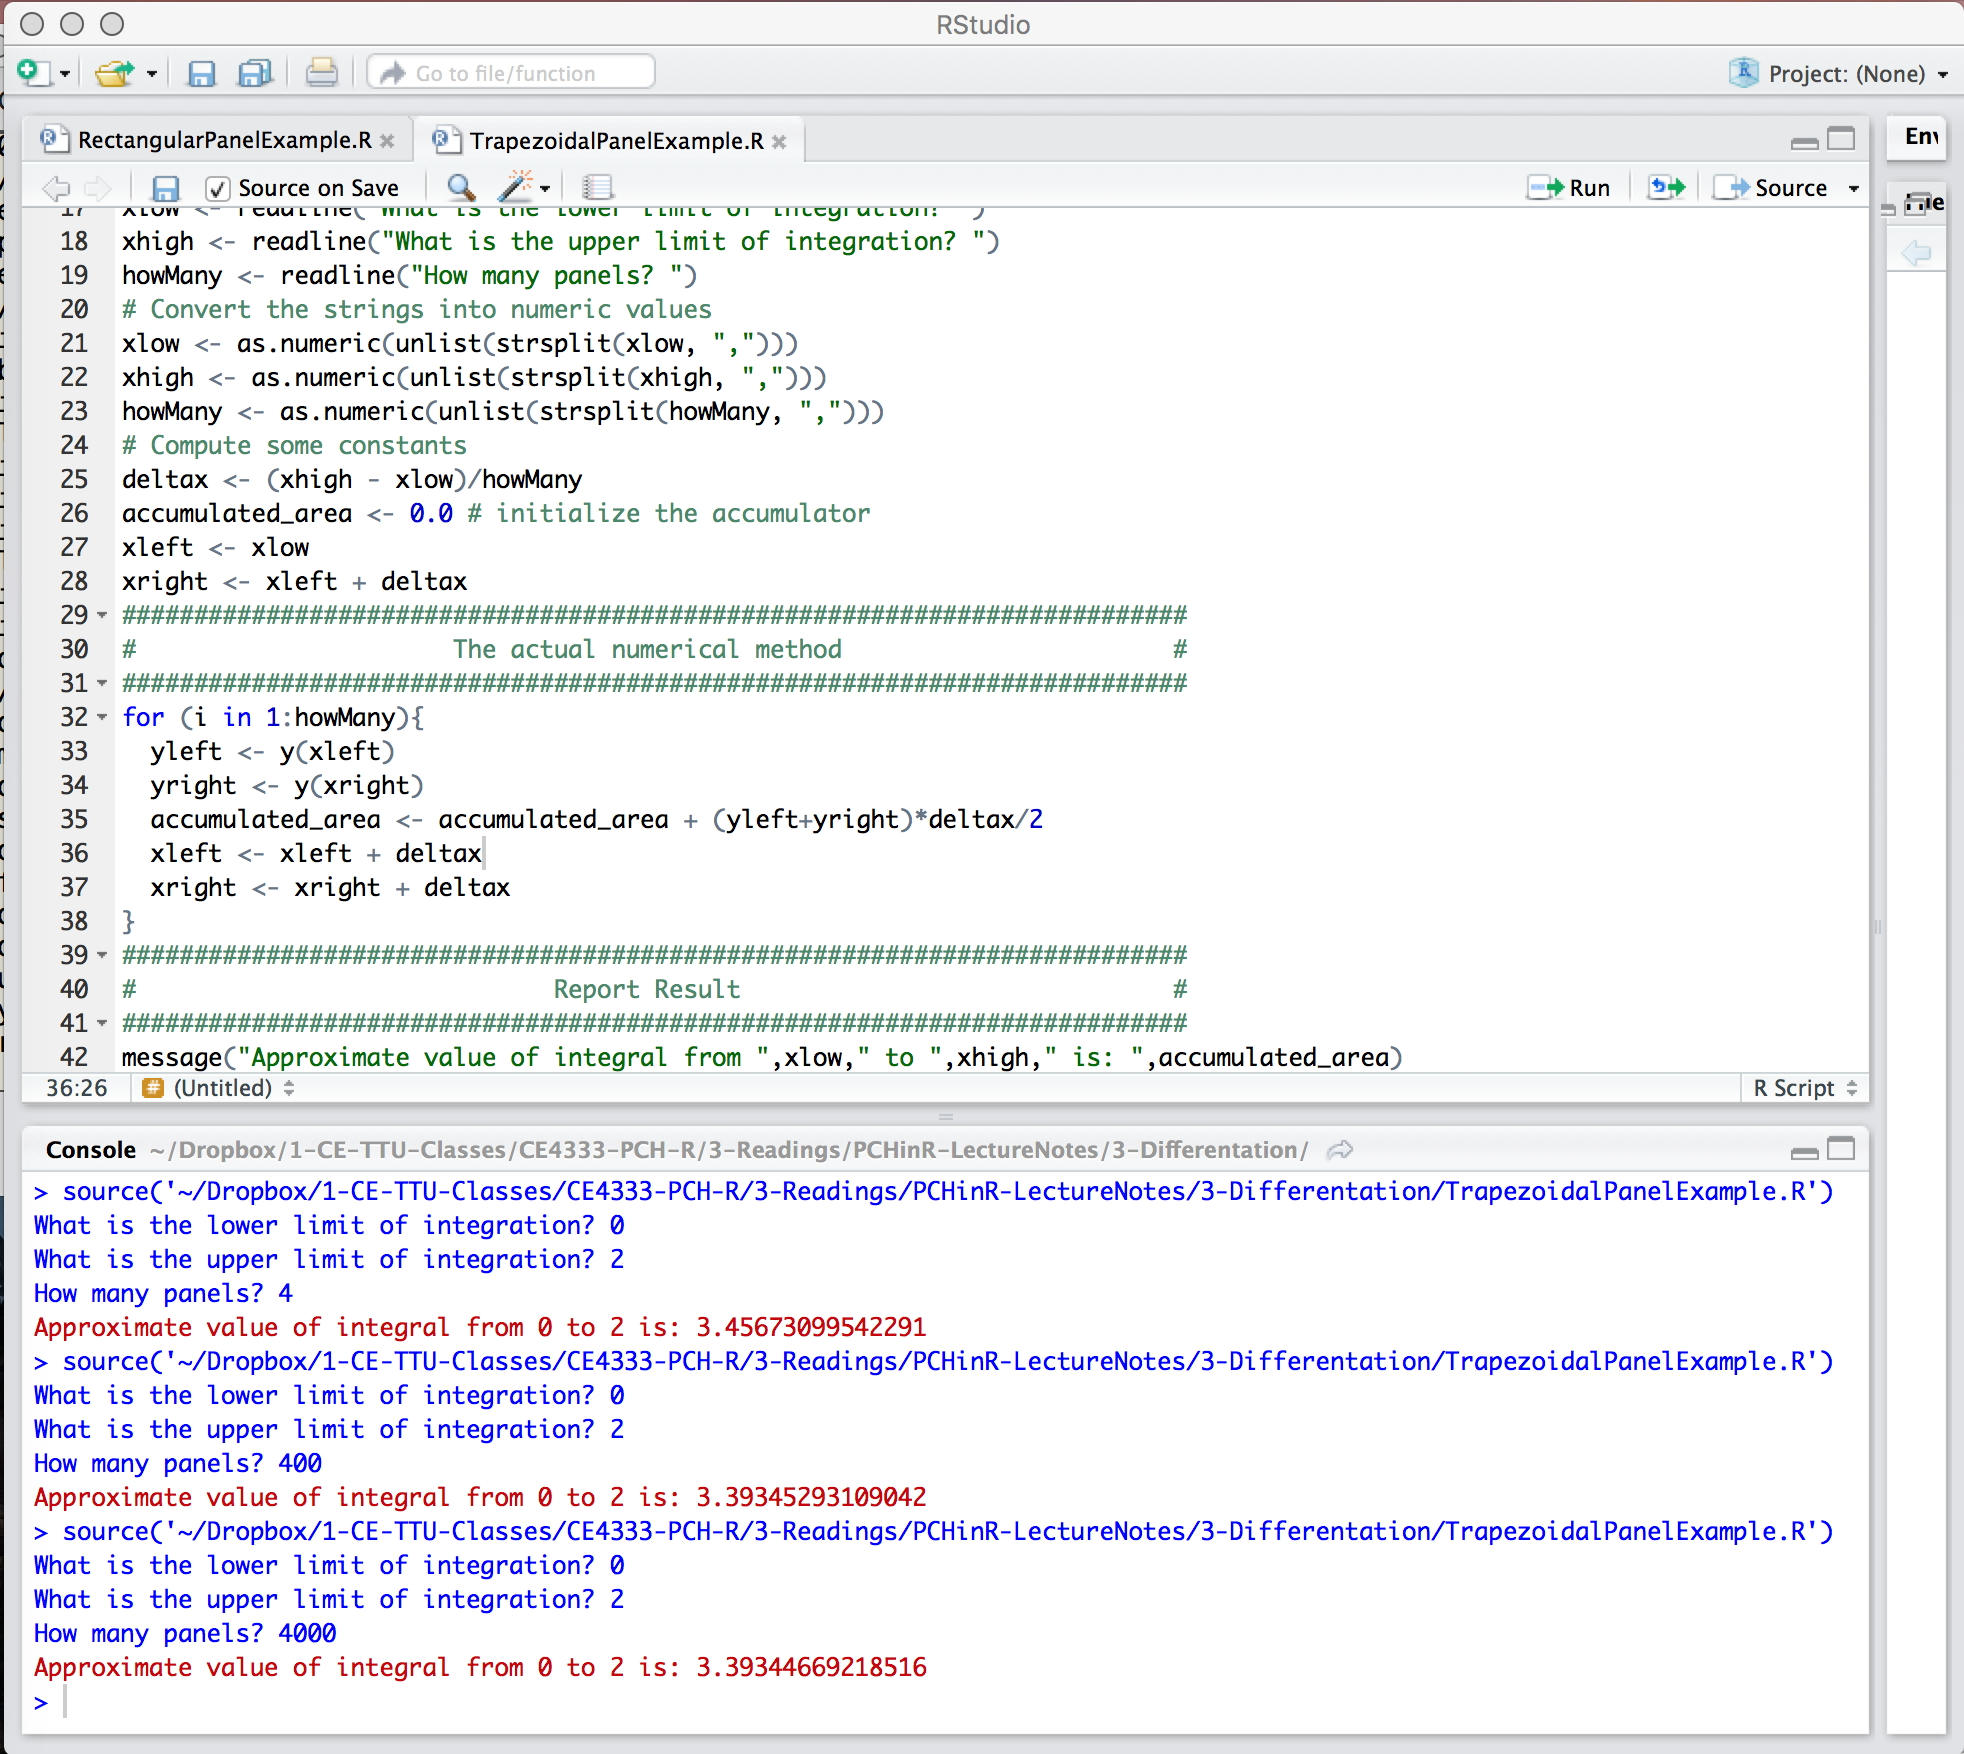
\includegraphics[width=6in]{./3-Differentation/TrapExample.jpg} 
   \caption{Trapezoidal panel example using 4, 400, and 4000 panels.}
   \label{fig:TrapExample}
\end{figure}

The actual listing depicted in Figure \ref{fig:TrapExample} is shown in Listing \ref{lst:TrapPanels}. 
Observe (at least for this example) the method appears more accurate that the rectangular method for the same number of panels, however also observe we are making twice as many function calls.
\clearpage

\begin{lstlisting}[caption=R code demonstrating Trapezoidal Panel Numerical Integration, label=lst:TrapPanels]
# R script to implement trapezoidal panel numerical integration
################################# NOTE ####################################
## The interactive input requires the script to be sourced                #
# In R console the command line would be                                  #
# source('PATH-TO-THE-FILE/TrapezoidalPanelExample.R')                    #
# where PATH-TO-THE-FILE is replaced with the actual path on your machine #
###########################################################################
#             Function to be integrated (modify as needed)                #
###########################################################################
y <- function(x){
  y <- x * sqrt(1+x^2)
  return(y)
}
###########################################################################
#             Get lower,upper and how many panels from user               #
###########################################################################
xlow <- readline("What is the lower limit of integration? ")  
xhigh <- readline("What is the upper limit of integration? ")
howMany <- readline("How many panels? ")
# Convert the strings into numeric values
xlow <- as.numeric(unlist(strsplit(xlow, ",")))
xhigh <- as.numeric(unlist(strsplit(xhigh, ",")))
howMany <- as.numeric(unlist(strsplit(howMany, ",")))
# Compute some constants
deltax <- (xhigh - xlow)/howMany  
accumulated_area <- 0.0 # initialize the accumulator
xleft <- xlow
xright <- xleft + deltax
##########################################################################
#                      The actual numerical method                       #
##########################################################################
for (i in 1:howMany){
  yleft <- y(xleft)
  yright <- y(xright)
  accumulated_area <- accumulated_area + (yleft+yright)*deltax/2
  xleft <- xleft + deltax
  xright <- xright + deltax
}
##########################################################################
#                             Report Result                              #
##########################################################################
message("Approximate value of integral from ",xlow," to ",xhigh," is: ",accumulated_area)
\end{lstlisting}

\subsubsection{Parabolic Panels}
Parabolic panels approximate the shape of the panel with a parabola.  The area between the chord and the curve (neglected in the trapezoidal solution) may be accounted for by approximating the function with a parabola passing through the points defined by three successive values of $y$.  

This area may be calculated from the geometry of the parabola and added to the trapezoidal area of the pair of strips to give the area $\Delta A$ of the pair as illustrated. Adding all of the $\Delta A$s produces the tabulation shown, which is known as Simpson's rule. To use Simpson's rule, the number $n$ of strips must be even.

\begin{figure}[h!] %  figure placement: here, top, bottom, or page
   \centering
   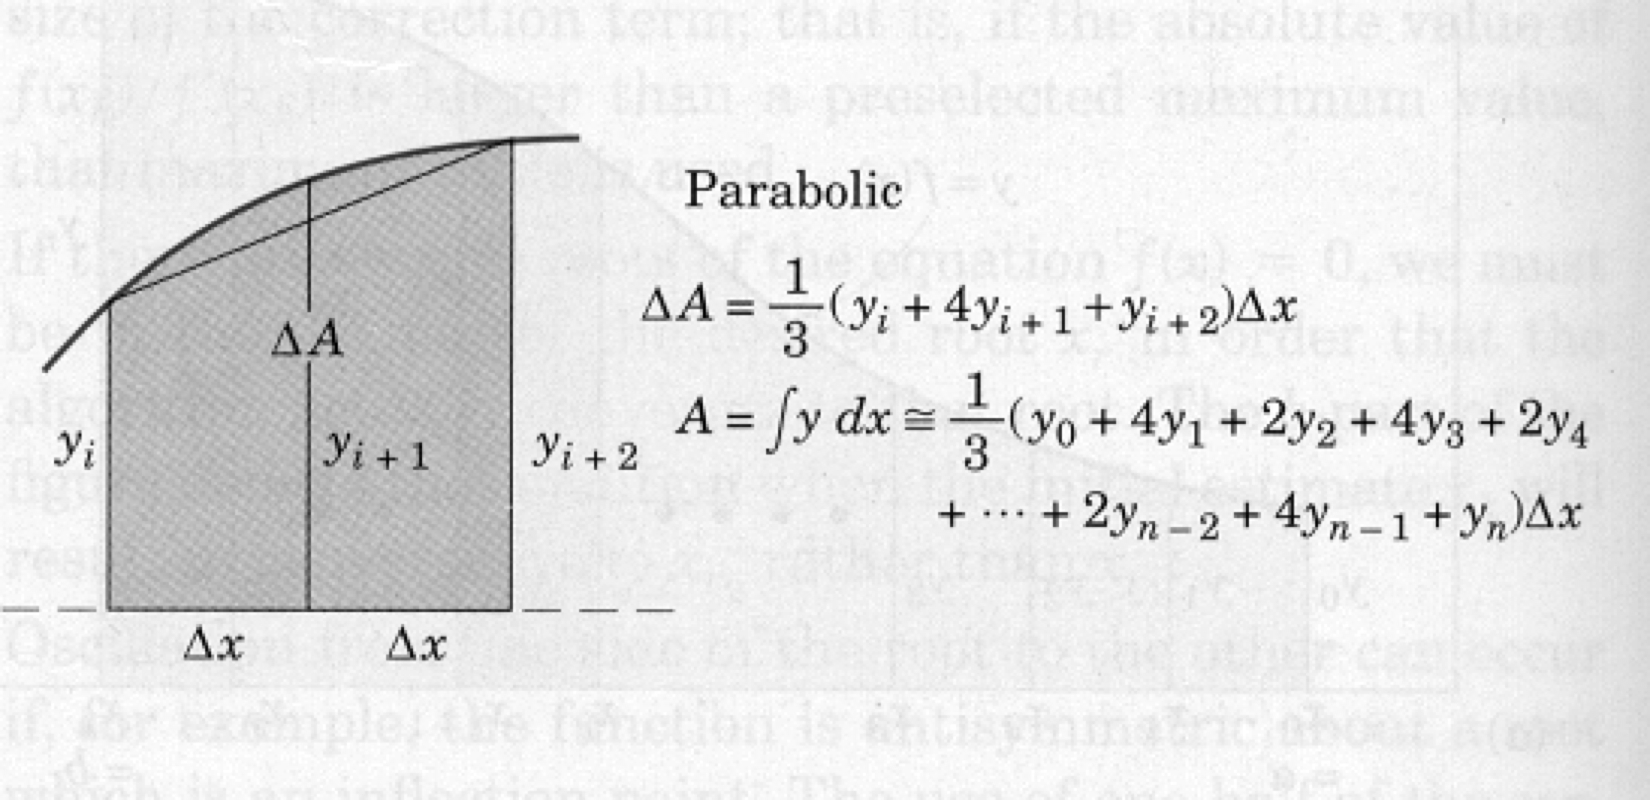
\includegraphics[width=5in]{./3-Differentation/ParabolicPanels.jpg} 
   \caption{Parabolic Panel Schematic.}
   \label{fig:ParabolicPanels}
\end{figure}

The same example as presented for rectangular panels is repeated, except using parabolic panels.  The code is changed yet again because we will evaluate at each end of the panel as well as at an intermediate value.

Figure \ref{fig:ParaExample} is a screen capture of a parabolic panel integration.   
The actual script is also listed in Listing \ref{lst:ParaPanels}. 
In the script, I substituted  $\frac{\Delta x}{2}$ for $\Delta x$ from Figure \ref{fig:ParabolicPanels}, so the accumulation line has a 6 in the denominator (rather than the 3 in the figure).\footnote{$\dots \frac{\Delta x}{2} \times \frac{1}{3}$ = $\dots \frac{\Delta x}{6}$}

\begin{figure}[h!] %  figure placement: here, top, bottom, or page
   \centering
   \includegraphics[width=6in]{./3-Differentation/ParaExample.jpg} 
   \caption{Parabolic panel example using 4, 400, and 4000 panels}
   \label{fig:ParaExample}
\end{figure}

Observe that the estimated integral for 400 and 4000 panels is nearly the same, suggesting no need to go beyond a certain number of panels.  
Algorithms that detect when to stop adding panels exist and would be implemented in many scientific and engineering programming applications.

\begin{lstlisting}[caption=R code demonstrating Parabolic Panel Numerical Integration, label=lst:ParaPanels]
# R script to implement trapezoidal panel numerical integration
################################# NOTE ####################################
## The interactive input requires the script to be sourced                #
# In R console the command line would be                                  #
# source('PATH-TO-THE-FILE/RectangularPanelExample.R')                    #
# where PATH-TO-THE-FILE is replaced with the actual path on your machine #
###########################################################################
#             Function to be integrated (modify as needed)                #
###########################################################################
y <- function(x){
  y <- x * sqrt(1+x^2)
  return(y)
}
###########################################################################
#             Get lower,upper and how many panels from user               #
###########################################################################
xlow <- readline("What is the lower limit of integration? ")  
xhigh <- readline("What is the upper limit of integration? ")
howMany <- readline("How many panels? ")
# Convert the strings into numeric values
xlow <- as.numeric(unlist(strsplit(xlow, ",")))
xhigh <- as.numeric(unlist(strsplit(xhigh, ",")))
howMany <- as.numeric(unlist(strsplit(howMany, ",")))
# Compute some constants
deltax <- (xhigh - xlow)/howMany  
accumulated_area <- 0.0 # initialize the accumulator
xleft <- xlow
xmiddle <- xleft + deltax/2
xright <- xleft + deltax
##########################################################################
#                      The actual numerical method                       #
##########################################################################
for (i in 1:howMany){
  yleft <- y(xleft)
  ymiddle <- y(xmiddle)
  yright <- y(xright)
  accumulated_area <- accumulated_area + (yleft+4*ymiddle+yright)*deltax/6
  xleft <- xright
  xmiddle <- xleft + deltax/2
  xright <- xleft + deltax
}
##########################################################################
#                             Report Result                              #
##########################################################################
message("Approximate value of integral from ",xlow," to ",xhigh," is: ",accumulated_area)
\end{lstlisting}

If we study all the forms of the numerical method we observe that the numerical integration method is really the sum of function values at specific locations in the interval of interest, with each value multiplied by a specific weight. 
In this development the weights were based on polynomials, but other method use different weighting functions.  
An extremely important method is called gaussian quadrature, which is outside the scope of the discussion herein  --- Gaussian quadrature routines are readily available within \textbf{R}.
The method is valuable because one can approximate convolution integrals quite effectively using quadrature routines, while the number of function evaluations for a polynomial based approximation could become hopeless.

When the function values are tabular, we are going to have to accept the rectangular (with adaptations) and trapezoidal as our best tool to approximate an integral because we don't have any really effective way to evaluate the function between the tabulated values --  if we were to use our interpolation routine from earlier, its really going to be a kind of trapezoidal rule anyway.

\clearpage
\subsection{Exercise Set 2}
\begin{enumerate}
\item Write a script to approximate $\int_{1.8}^{3.4}e^x dx$ using rectangular panels.  \\Run your script using 6 and 600 panels.  
\begin{enumerate}
\item What is the analytical solution (e.g. do the calculus!)?  
\item What is the percent error between the analytical solution and the approximation using 6 panels?
\item What is the percent error between the analytical solution and the approximation using 600 panels?
\end{enumerate}
\item Write a script to approximate $\int_{1.8}^{3.4}e^x dx$ using trapezoidal panels.   \\Run your script using 6 and 600 panels.  
\begin{enumerate}
\item What is the analytical solution (e.g. do the calculus!)?  
\item What is the percent error between the analytical solution and the approximation using 6 panels?
\item What is the percent error between the analytical solution and the approximation using 600 panels?
\end{enumerate}
\item Based on the previous two exercises, which method do you think is more accurate for a given panel count?  Why (do you think so)?
\item Write a script to approximate $\int_{0}^{1}ln(x) dx$ using rectangular panels.  \\Run your script using 6 and 600 panels.  
\begin{enumerate}
\item What is the analytical solution (e.g. do the calculus!)?  
\item What is the percent error between the analytical solution and the approximation using 6 panels?
\item What is the percent error between the analytical solution and the approximation using 600 panels?
\end{enumerate}

\item Write a script to approximate $\int_{0}^{1}ln(x) dx$ using trapezoidal panels.  \\Run your script using 6 and 600 panels.  
\begin{enumerate}
\item Did you get an error message --- why?
\end{enumerate}

\end{enumerate}

This exercise set is also located on the class server as \texttt{ES-2}
\clearpage

\subsection{Numerical Integration of Tabular Data}
This subsection is going to work with tabular data --- different from function evaluation, but similar.  
To be really useful, we need to learn how to read data from a file --- manually entering tabular data is really time consuming, error prone, and just plain idiotic.

So in this subsection we will first learn how to read data from a file into a list, then we can process the list as if it were a function and integrate its contents.   %I am probably going to dispense with cuteness for awhile --- file reads and writes are complex in any language, so you have to adult (as a verb) for a little while --- sorry!

\subsubsection{Reading from a file -- open, read, close files}
\textbf{R} can read from an ASCII file (or even an Excel .csv file) using a multitude of methods.  Common methods are \texttt{read.table(\dots )}, \texttt{read.table(\dots )}, \texttt{read.table(\dots )}, \texttt{read.table(\dots )}, and \texttt{read.table(\dots )}.

One can also use primatives\footnote{Jargon to describe lower level tools within \textbf{R}} to read individual rows in a file and process them.\footnote{We will use this approach later in the book -- the interactive prompt and reads in the prior subsection are similar to this approach where input is read into a string, then the string is converted into the appropriate type of object (numeric or text).}

First, lets create a file named \texttt{MyFile.txt}.
The extension is important so that we can examine the file with other tools (a text editor) and remember that it is an ASCII file.
The contents of \texttt{MyFile.txt} are:
\begin{verbatim}
1 , 1
2 , 4
3 , 9
4 , 16
5 , 25
\end{verbatim}

To read the contents into an \textbf{R} script we have to do the following:
\begin{enumerate}
\item Open a connection to the file --- this is a concept common to all languages, it might be called something different, but the program needs to somehow know the location and name of the file.
\item Read the contents into an object --- we have a lot of control on how this gets done, for the time being we won't exercise much control yet.  When you do substantial programs, you will depend on the control of the reads (and writes).
\item Disconnect the file --- this too is common to all languages.  Its a really easy step to forget.  Not a big deal if the program ends as planned but terrible if there is a error in the program and the connection is still open.  Usually noting bad happens, but with an open connection it is possible for the file to get damaged.   If that file represents millions of customers data, that's kind of a problem.
\end{enumerate}
\newpage
The \texttt{read.table} class of functions handles all three of these steps for us, we do have to provide the filename and some information about the file structure.  Later when we are doing network simulation and other hydraulic techniques, different parts of an input file will be read line-by-line and processed --- for this task we will need to handle these three steps using primatives.

Figure \ref{fig:ReadMyFile} illustrates the process.  The input file has 5 lines, these get read then echoed (printed) back to us.  The actual script is pretty simple, notice how the \texttt{filepath} and \texttt{filename} character variables are defined, then pasted together to produce a full \textit{absolute} file name.\footnote{A file name can specify all the directory names starting from the root of the tree; then it is called an absolute file name. Or it can specify the position of the file in the tree relative to a default directory; then it is called a relative file name. On the computer I used to write this workbook, the symbol \~ ~, is the root to my user account, then the remaining directories from that location are explicitly listed.  The actual absolute name is 
/Users/cleveland/Dropbox/1-CE-TTU-Classes/CE4333-PCH-R/3-Readings/PCHinR-LectureNotes/3-Differentation/RScripts}

Listing \ref{lst:ReadMyFile} is a listing of the script used in Figure \ref{fig:ReadMyFile}.  
The analyst should be able to deduce that the filenames could be read from user input using the prompting technique used in the earlier subsections, so if one is going to process a lot of similar files the explicit naming could be replaced with variable naming -- it would probably be a good idea to confine the files to a reasonably memorable path.

\begin{figure}[h!] %  figure placement: here, top, bottom, or page
   \centering
   \includegraphics[width=6in]{./3-Differentation/ReadMyFile.jpg} 
   \caption{Rudimentary file reading}
   \label{fig:ReadMyFile}
\end{figure}

\begin{lstlisting}[caption=R code demonstrating Reading from a File, label=lst:ReadMyFile]
# R script to illustrate reading from a file using read.table
# The script is intentionally complicated to illustrate the 
# three steps: open connection, read into object, close connection
filepath <- "~/Dropbox/1-CE-TTU-Classes/CE4333-PCH-R/3-Readings/PCHinR-LectureNotes/3-Differentation/RScripts"
filename <- "MyFile.txt"
fileToRead <- paste(filepath,filename,sep="/") # build the user absolute filename
# Here we open the connection to the file (within read.table)
# Then the read.table attempts to read the entire file into an object named zz
# Upon either fail or success, read.table closes the connection
zz <- read.table(fileToRead,header=FALSE,sep=",") # comma seperated ASCII, No header
# Echo zz 
print(zz)
\end{lstlisting}

Now that we can read a file,  we are now able to integrate tabular data.

\subsection{Integrating tabular data}
Suppose instead of a function we only have tabulations and wish to estimate the area under the curve represented by the tabular values.  Then our integration rules from the prior sections still work more or less, except the rectangular panels will have to be shifted to either the left edge or right edge of a panel (where the tabulation exists).   

Lets just examine an example.  Suppose some measurement technology produced Table \ref{tab:MyIntegralTable} a table of related values.   The excitation variable is $x$ and $f(x)$ is the response.   

% Requires the booktabs if the memoir class is not being used
\begin{table}[h!]
   \centering
   \caption{Tabular values of an excitation--response relationship}
   \begin{tabular}{p{1in}p{1in}} 
   $x$ & $f(x)$ \\
   \hline
   \hline
   1.0 & 1.543 \\
   1.1 & 1.668 \\
   1.2 & 1.811 \\
   1.3 & 1.971 \\
   1.4 & 2.151 \\
   1.5 & 2.352 \\
   1.6 & 2.577 \\
   1.7 & 2.828 \\
   1.8 & 3.107 \\
   \hline
   \end{tabular}
   \label{tab:MyIntegralTable}
\end{table}

To integrate this table using the trapezoidal method is straightforward.  We will modify our earlier code to read the table (which we put into a file), and compute the integral.  

Figure \ref{fig:MyTrapTab} is a screen capture of a script that implements the file read and the numerical integration.
The conversion of the method from the functional form in the previous section is pretty straightforward.  
The main nusiance here is the syntax required to access the ``x'' values and the ``y'' values.   
In \textbf{R} the most generic approach is \texttt{object\$name}, where \textit{object} is the data frame name, and \textit{name} is the variable (column) name.  If you don't use headers, \textbf{R} assigns names as \texttt{V1,V2,\dots,V$_{max}$}.   

\begin{figure}[h!] %  figure placement: here, top, bottom, or page
   \centering
   \includegraphics[width=6in]{./3-Differentation/MyTrapTab.jpg} 
   \caption{Integrating tabular data.}
   \label{fig:MyTrapTab}
\end{figure}

Realistically the only other simple integration method for tabular data is the rectangular rule, either using the left edge of a panel or the right edge of a panel (and you could do both and average the result which would result in the same outcome as the trapezoidal method).   For the sake of completeness lets do both and then compare the results from all four approaches (trapezoidal, rectangular-left, rectangular-right, average rectangular).

First, Figure \ref{fig:MyRectLeft} implements the file read and tabular integration using the rectangular panel method, evaluating the function at the left edge of each panel.

\begin{figure}[h!] %  figure placement: here, top, bottom, or page
   \centering
   \includegraphics[width=6in]{./3-Differentation/MyRectLeft.jpg} 
   \caption{Integrating tabular data.   Rectangular panel, evaluate at left edge.}
   \label{fig:MyRectLeft}
\end{figure}

Next, Figure \ref{fig:MyRectRight} implements the file read and tabular integration using the rectangular panel method, evaluating the function at the left edge of each panel.

Now lets compare the results from using the three (four) approaches.  Table \ref{tab:MyTabularMethodCompare} are the results by method.   
% Requires the booktabs if the memoir class is not being used
\begin{table}[h!]
   \centering
   \caption{Comparison of tabular integration}
   \begin{tabular}{p{2.5in}p{2in}} 
   Method & Computed Area \\
   \hline
   \hline
Trapezoidal Panels & 1.7683 \\
Rectangular - Left Edge & 1.6901 \\
Rectangular - Right Edge & 1.8465 \\
Arithmetic Mean Rectangular & 1.7683  \\
   \hline
   \end{tabular}
   \label{tab:MyTabularMethodCompare}
\end{table}

What Table \ref{tab:MyTabularMethodCompare} illustrates is that the trapezoidal rule is simply the average of the rectangular rule evaluated at first the left-edge then the right-edge of a panel.   

\begin{figure}[t!] %  figure placement: here, top, bottom, or page
   \centering
   \includegraphics[width=6in]{./3-Differentation/MyRectRight.jpg} 
   \caption{Integrating tabular data.   Rectangular panel, evaluate at right edge.}
   \label{fig:MyRectRight}
\end{figure}

%\subsection{Exercises}
%\begin{enumerate}
%\item Approximate $\int_0^2 f(x) dx$ from the tabulation in Table \ref{tab:IntegrateThisProblem}.
%% Requires the booktabs if the memoir class is not being used
%\begin{table}[h!]
%   \centering
%   \caption{Tabular values of a function -- non-uniform spacing in $x$}
%   \begin{tabular}{p{1in}p{1in}} 
%   $x$ & $f(x)$ \\
%   \hline
%   \hline
%   0.00 & 1.0000 \\
%   0.12 & 0.8869 \\
%   0.53 & 0.5886 \\
%   0.87 & 0.4190 \\
%   1.08 & 0.3396 \\
%   1.43 & 0.2393 \\
%   2.00 & 0.1353 \\
%   \hline
%   \end{tabular}
%   \label{tab:IntegrateThisProblem}
%\end{table}
%\newpage
%\item Table \ref{tab:HyperbolicCosine} is a tabulation of various values of the hyperbolic cosine function.   
%\begin{enumerate}
%\item Approximate $\int_1^{9.0} f(x) dx$ from the tabulation in Table \ref{tab:HyperbolicCosine}.
%\item Approximate $\int_1^{4.2} f(x) dx$ from the tabulation in Table \ref{tab:HyperbolicCosine}.
%\item Approximate $\int_1^{4.0} f(x) dx$ from the tabulation in Table \ref{tab:HyperbolicCosine}.
%\item Briefly explain how you choose to handle starting and stopping the integration from values that are intermediate and within the tabulation.
%\item Also explain how you choose to handle  working with values that fall between tabulated values.
%\end{enumerate}
%\begin{table}[h!]
%   \centering
%   \caption{Tabular values of the hyperbolic cosine}
%   \begin{tabular}{p{1in}p{1in}} 
%   $x$ & $f(x)$ \\
%   \hline
%   \hline
%1.0 & 1.54308063481524 \\
%1.1 & 1.66851855382226 \\
%1.2 & 1.81065556732437 \\
%1.3 & 1.97091423032663 \\
%1.4 & 2.15089846539314 \\
%1.5 & 2.35240961524325 \\
%1.6 & 2.57746447119489 \\
%1.7 & 2.82831545788997 \\
%1.8 & 3.10747317631727 \\
%2.0 & 3.76219569108363 \\
%2.2 & 4.56790832889823 \\
%2.4 & 5.55694716696551 \\
%2.6 & 6.76900580660801 \\
%2.8 & 8.25272841686113 \\
%3.0 & 10.0676619957778 \\
%3.3 & 13.5747610440296 \\
%3.6 & 18.3127790830626 \\
%3.9 & 24.711345508488 \\
%4.2 & 33.3506633088728 \\
%4.6 & 49.7471837388392 \\
%5.0 & 74.2099485247878 \\
%5.5 & 122.348009517829 \\
%6.0 & 201.715636122456 \\
%7.0 & 548.317035155212 \\
%8.0 & 1490.47916125218 \\
%9.0 & 4051.54202549259 \\
%   \hline
%   \end{tabular}
%   \label{tab:HyperbolicCosine}
%\end{table}
%\end{enumerate}
%%%%%%%%%%%%%%%%%%%%%%%%%%%%%%%%%%%%%%%%%%%%%%%%%%%%%%%%
%%%%%%%%%%%%%%%%%%%%%%%%%%%%%%%%%%%%%%%%%%%%%%%%%%%%%%%%
\subsection{Numerical Differentiation}
Similar in context to numerical integration is approximation of derivatives.   
If the functions are representable as functions, then differencing degenerates into the selection of an appropriate difference formula.
If the function is tabular, the same decision is presented, but we have to pay additional attention to the quantity of observations available.

\subsection{Difference Approximations for Tabulated Data}
Here we will introduce differencing by an example.
Suppose we want to convert a cumulative data series into an incremental data series.  
It is operationally related to numerical differentiation.   

As an example (leading to an algorithm) consider the cumulative rainfall time series in Table \ref{tab:cumulative_rainfall_timeseries}.

We shall import this data into \textbf{R}, then plot the data, then construct a computational procedure to extract the incremental values from the cumulative values.
To load the data into \textbf{R} we start the program and then read the contents of a data file that contains the data into \textbf{R}, then we will introduce the plotting tools in \textbf{R}.
In addition to plotting, we will also learn about headers and attaching an object (which gives access to header names rather than the \texttt{object\$name} structure.

% Requires the booktabs if the memoir class is not being used
\begin{table}[ht!]
\centering
\caption{Cumulative Rainfall Time Series}
\begin{tabular}{cc} % Column formatting, @{} suppresses leading/trailing space
~&~\\
  hours & cumulative\_rain\\
  0.0&0.00\\
  0.5&1.06\\
  1.0&2.99\\
 1.5&4.80\\
 2.0&4.80\\
 2.5&4.80\\
 3.0&4.80\\
 3.5&4.80\\
 4.0&4.80\\
 4.5&4.80\\
 5.0&4.80\\
 5.5&4.80\\
\end{tabular}
\label{tab:cumulative_rainfall_timeseries}
\end{table}


\begin{figure}[htbp] %  figure placement: here, top, bottom, or page
   \centering
   \includegraphics[width=6in]{./3-Differentation/cumulative_rain_plot.jpg} 
   \caption{Plot of Cumulative Rainfall Time Series}
   \label{fig:cumulative_rain_plot}
\end{figure}

The plot suggests that the values are accumulated at the end of the time interval, thus the value accumulated is some average ``rate'' multiplied by the time interval.  
The line segment between each point is called a ``secant'' line.  
The slope of each secant line, provides that average ``rate''.  
So a fundamental computational step will be a function that computes the slope given any two points (assumed to be adjacent --- so that's why sorting can become important, although the program doesn't actually care).

\subsubsection{Slope of a Secant Line}
\texttt{slopeOfSecant} is a prototype function that we write to that computes the slope of the secant line through two known points on a function $f(x_1)$ and $f(x_2)$.  The function could be tabular or evaluated.  The script assumes tabular in that the function is evaluates external to \texttt{slopeOfSecant}.  

\begin{lstlisting}[caption=R code demonstrating the prototype function \texttt{slopeOfSecant} , label=lst:SlopeOfSecant]
############## slope function prototype ####################
slopeOfSecant<-function(f1,f2,x1,x2){
  slopeOfSecant <- (f2-f1)/(x2-x1);
  return(slopeOfSecant)
}
#######################################################
\end{lstlisting}

This slope is also a first order approximation of a derivative (forward, backward, and centered differences depending on values supplied).  This function can then be used to compute ``derivatives'' of data series using a disaggregation function.

As an illustrative example, if we present parts of the cumulative rainfall data series we can recover the average rate between the inputs.  Figure \ref{fig:addSecant} is a screen capture of such a test.

\begin{figure}[htbp] %  figure placement: here, top, bottom, or page
   \centering
   \includegraphics[width=6in]{./3-Differentation/addSecant.jpg} 
   \caption{Script with slopeOfSecant prototype inserted and validation that we recover rate and can re-accumulate correctly}
   \label{fig:addSecant}
\end{figure}

\subsubsection{Disaggregation}
\texttt{disaggregate} is a prototype function that computes the slopes of the secant lines joining adjacent pairs of input data.  Depending on the way the input arrays are presented to the \texttt{disaggregate} function, the function returns either the backward difference approximation to the function's derivative or if an index is presented instead of actual $t$ values, then the function returns the incremental values that when aggregated reconstruct the original input function.

\begin{lstlisting}[caption=R code demonstrating the prototype function \texttt{disaggregate()} , label=lst:Disaggregate]
########      disaggregate function prototype    ###########
# returns a vector of slopes computed by sloepOfSecant 
disaggregate<-function(f,x,dfdx){
  n<-length(x) # length of vectors
  dfdx<-rep(0,n); # zero dfdx
  for (i in 2:n){dfdx[i]<-slopeOfSecant(f[i-1],f[i],x[i-1],x[i]);};
  dfdx[1]<-0;
  return(dfdx)} 
############################################################
\end{lstlisting}

\subsubsection{Numerical Differentiation}

A related concept is to determine the average rate for the time interval, the principal difference is that the rate occurs during the entire time interval and should be assigned to the beginning of the interval instead of the end of the interval.  A subtle change in the \texttt{disaggregate} function can accomplish the task, we will name that new function \texttt{brbt}.  The name is a nemonic for ``backward-rate, backward-time'' differencing.

\begin{lstlisting}[caption=R code demonstrating the prototype function \texttt{brbt()} , label=lst:BrBt]
########### backward rate, backward time prototype ###########
brbt<-function(f,x,dfdx){
  n<-length(x) # length of vectors
  dfdx<-rep(0,n); # zero dfdx
  for (i in 1:(n-1)){dfdx[i]<-slopeOfSecant(f[i],f[i+1],x[i],x[i+1]);};
  dfdx[n]<-0;
  return(dfdx)}
############################################################
\end{lstlisting}

Finally, putting everything together, we have the toolkit to determine the incremental rates (which is an approximation to the derivative of the cumulative rates) and incremental depths which are these individual rates multiplied by the length of the time interval.
Figure \ref{fig:processed_rain_plot} is a screen capture of the \textbf{R} script that implements these functions on the tabular data.

\begin{figure}[h!] %  figure placement: here, top, bottom, or page
   \centering
   \includegraphics[width=6in]{./3-Differentation/processed_rain_plot.jpg} 
   \caption{Plot of Cumulative Rainfall Time Series (BLUE), Incremental Depth Time Series (GREEN), and Average Rate Time Series (RED)}
   \label{fig:processed_rain_plot}
\end{figure}

Listing \ref{lst:NumDifferencing} is a listing of the \textbf{R} script that produced Figure \ref{fig:processed_rain_plot}.  
The intermediate steps from Figure \ref{fig:addSecant} is removed in this listing.

\begin{lstlisting}[caption=R code demonstrating Numerical Differencing , label=lst:NumDifferencing]
# R script to illustrate numerical differencing 
rm(list=ls()) # clear all objects
############ Prototype (forward define) Functions #########
############## slope function prototype ####################
slopeOfSecant<-function(f1,f2,x1,x2){
  slopeOfSecant <- (f2-f1)/(x2-x1);
  return(slopeOfSecant)}
########      disaggregate function prototype    ###########
disaggregate<-function(f,x,dfdx){
  n<-length(x) # length of vectors
  dfdx<-rep(0,n); # zero dfdx
  for (i in 2:n){dfdx[i]<-slopeOfSecant(f[i-1],f[i],x[i-1],x[i]);};
  dfdx[1]<-0;
  return(dfdx)} 
########### backward rate, backward time prototype ###########
brbt<-function(f,x,dfdx){
  n<-length(x) # length of vectors
  dfdx<-rep(0,n); # zero dfdx
  for (i in 1:(n-1)){dfdx[i]<-slopeOfSecant(f[i],f[i+1],x[i],x[i+1]);};
  dfdx[n]<-0;
  return(dfdx)}
##############################################################

################ Build the filename #########################
filepath <- "~/Dropbox/1-CE-TTU-Classes/CE4333-PCH-R/3-Readings/PCHinR-LectureNotes/3-Differentation/RScripts"
filename <- "cumulative_rainfall.txt"
fileToRead <- paste(filepath,filename,sep="/") # build the user absolute filename
# Here we open the connection to the file (within read.table)
# Then the read.table attempts to read the entire file into an object named zz
# Upon either fail or success, read.table closes the connection
zz <- read.table(fileToRead,header=TRUE,sep=",") # comma seperated ASCII, No header
attach(zz) # attach associates the column names with the data below them.
## summary(zz) # useful to be sure data were imported correctly
incremental_depth <- disaggregate(cumulative_rain,hours,dfdx)
incremental_rate <- brbt(cumulative_rain,hours,dfdx)
dt <- 0.5 # how long each interval, make adaptive as exercise
incremental_depth <- incremental_depth*dt
print(cbind(zz,incremental_rate,incremental_depth))
################ Build the Plot #####################################
plot(hours,cumulative_rain,xlab="Time(hours)",ylab="Cumulative Depth 
(inches)",type="l",lwd=5,col="Blue",tck=1)
lines(hours,incremental_depth*dt,pch=16,col="green",lwd=3)
lines(hours,incremental_rate,pch=16,col="red",lwd=2,type="s")
text(3,4.1,"Cumulative Rain",col="blue")
text(3,3.1,"Incremental Rain",col="green")
text(3,2.1,"Incremental Rate",col="red")
#####################################################################
detach(zz) #deallocate the zz object
\end{lstlisting}

\subsubsection{Aggregation}
Aggregation is the compliment of disaggregation; instead of finding differences we are trying to produce cumulatives from incremental values or rates.  Aggregation is to integration as disaggregation is to differentiation.  Simple aggregation functions are straightforward to build.  Numerical integration (already introduced) is a bit more challenging because there are many different ways to compute areas from tabular data -- we will illustrated rectangular, trapezoidal, and parabolic panels.  

We can insert a prototype \texttt{aggregate} function that simply adds elements in a series to prior elements and stores the value in another series.  Another name for this kind of arithmetic is a running sum.   Functionally, it is rectangular panel (evaluate from the left), numerical integration.
 
\begin{lstlisting}[caption=R code demonstrating the prototype function \texttt{aggregate()} , label=lst:aggregate]
########### aggregate function prototype ###########
aggregate<-function(vector1,vector2){
n<-length(vector1)
# fill vector2 with zeros
vector2<-rep(0,n)
vector2[1]<-vector1[1]+0.0
for(i in 2:n)vector2[i]<-vector2[i-1]+vector1[i]
return(vector2)}
###############################################
\end{lstlisting}

We add this function to the prototype list ate the top of the script and can run
To illustrate the use of \texttt{aggregate} we will aggregate the incremental depths into the cumulative rainfall -- we should recover the original cumulative rainfall series that was originally supplied.

\subsection{Exercises}
\begin{enumerate}
\item Add the \texttt{aggregate} prototype function to collection of prototype functions in the script.
The add some code like:
\begin{verbatim}
new_cum_rain<-aggregate(incremental_depth,dummy)
plot(hours,cumulative_rain,xlab="Time(hours)",ylab="Cumulative Depth
(inches)",type="l",lwd=5,col="Blue",tck=1)
lines(hours,new_cum_rain,col="red",lwd=1.5)
\end{verbatim}
Demonstrate that the two series are identical (e.g. plotting on top of one another).
\item (Advanced) Modify the \texttt{disaggregate()} prototype function to automatically determine the time spacing ($x$) and perform the correct multiplication within the function to return the correct increments.
You only have to add one line of code to the prototype function at
\begin{verbatim}
for (i in 2:n){dfdx[i]<-slopeOfSecant(f[i-1],f[i],x[i-1],x[i]);
	deltax <-   # you need to define this in terms of x[i] and x[i-1]!
	dfdx[i]<- deltax*dfdx[i];};
\end{verbatim}
\end{enumerate}

\subsection{Finite-Difference Formulas}
What we have just done is to explore the use of finite-difference approximations for derivatives. 
Some common formulas for difference formulas are listed below (without derivation -- you should be able to find explanation in any numerical methods text).
All the difference equations presented here are the result of truncated Taylor series expansions about $x$.
The ``order'' refers to the magnitude of truncation error, and this magnitude is proportional to the step size ($\Delta x$) raised to a power (the order).   
Truncation error decreases as the step size is decreased, but one is approaching a divide-by-zero situation (because numerical methods don't do limits just yet!).
\subsubsection{First Derivatives}
Equation \ref{eqn:1st-back} is a first-order backwards difference.
\begin{equation}
\frac{df}{dx} \approx~ \frac{f(x) - f(x -\Delta x)}{\Delta x}
\label{eqn:1st-back}
\end{equation}
Equation \ref{eqn:1st-forward} is a first-order backwards difference.
\begin{equation}
\frac{df}{dx}  \approx~ \frac{f(x + \Delta x) - f(x)}{\Delta x}
\label{eqn:1st-forward}
\end{equation}
Equation \ref{eqn:1st-center} is a second-order central difference.
\begin{equation}
\frac{df}{dx}  \approx~ \frac{f(x + \Delta x) - f(x -\Delta x)}{2 \Delta x}
\label{eqn:1st-center}
\end{equation}
\subsubsection{Second Derivatives}
Equation \ref{eqn:2nd-center} is a second-order central difference.
\begin{equation}
\frac{d^2f}{dx^2}  \approx~ \frac{f(x + \Delta x) - 2f(x) + f(x -\Delta x)}{ \Delta x^2}
\label{eqn:2nd-center}
\end{equation}

\subsubsection{Third Derivatives}
Equation \ref{eqn:3nd-center} is a sixth-order central difference.
\begin{equation}
\frac{d^3f}{dx^3}  \approx~ \frac{f(x + 2\Delta x) -2f(x + \Delta x) + 2f(x -\Delta x) + f(x -2\Delta x)}{ 2 \Delta x^3}
\label{eqn:3nd-center}
\end{equation}

The procedure to generate such difference formulas is general and can supply estimates with approximations of any degree.  
The accuracy depends on the location and number of field variable values involved in the approximation.  
The selection of a formula is not at all trivial (especially with tabulations), but beyond the scope of this handbook.

Despite known complications, this is a general tool used in computational hydraulics and we will use it throughout the remainder of the handbook -- in some examples it will not be obvious that it is finite differencing, and in others it will be explicitly obvious.
The next section introduces Newton's method, and finite-differences will be used to approximate the derivative (Quasi-Newton) to implement the method.  The procedure is really quite common and imbedded in a lot of the computational tools we use professionnaly.
\clearpage

\subsection{Single Variable Quasi-Newton Methods}
%Single variable minimization and root finding are similar numerical exercises.
%Both activities are aimed at finding solutions to the equation $f(x) = 0$, although minimization may not necessarily solve such an equation.\footnote{In essence, root finding can be posed as a minimization problem, but the converse is not true}

The application of fundamental principles of modeling and mechanics often leads to an algebraic or transcendental equation that cannot be easily solved and represented in a closed form.  
In these cases a numerical method is required to obtain an estimate of the root or roots of the expression.  

Newton's method is an iterative technique that can produce good estimates of solutions to such equations.  
The method is employed by rewriting the equation in the form $f(x)=0$, then successively manipulating guesses for $x$ until the function evaluates to a value close enough to zero for the modeler to accept.
  
Figure \ref{fig:ArbitraryFunction} is a graph of some function whose intercept with the $x-$axis is unknown.  
The goal of Newton's method is to find this intersection (root) from a realistic first guess.  
Suppose the first guess is $x_1$, shown on the figure as the right-most specific value of $x$. 
The value of the function at this location is $f(x_1)$.  
Because $x_1$ is supposed to be a root the difference from the value zero represents an error in the estimate.  
Newton's method simply provides a recipe for corrections to this error.  

\begin{figure}[h!] %  figure placement: here, top, bottom, or page
   \centering
   \includegraphics[width=4in]{./3-Differentation/ArbitraryFunction.jpg} 
   \caption{Graph of Arbitrary Function.}
   \label{fig:ArbitraryFunction}
\end{figure}

Provided $x_1$ is not near a minimum or maximum (slope of the function is not zero) then a better estimate of the root can be obtained by extending a tangent line from $x_1,f(x_1)$ to the $x$-axis.  
The intersection of this line with the axis represents a better estimate of the root.

This new estimate is $x_2$.  
A formula for $x_2$ can be derived from the geometry of the triangle $x_2$,$f(x_1)$,$x_1$.   
Recall from calculus that the tangent to a function at a particular point is the first derivative of the function.  
Therefore, from the geometry of the triangle and the definition of tangent we can write,
\begin{equation}
tan(\theta)=\frac{df}{dx}\Biggr\vert_{x_1} = \frac{f(x_1)}{x_1 - x_2}
\end{equation}

Solving the equation for $x_2$ results in a formula that expresses $x_2$ in terms of the first guess plus a correction term.
\begin{equation}
x_2=x_1 - \frac{f(x_1)}{\frac{df}{dx}\vert_{x_1}} 
\end{equation}

The second term on the right hand side is the correction term to the estimate on the right hand side.  
Once $x_2$ is calculated we can repeat the formula substituting $x_2$ for $x_1$ and $x_3$ for $x_2$ in the formula.  
Repeated application usually leads to one of three outcomes:
\begin{enumerate}
\item a root;
\item divergence to $\pm\infty$; or 
\item cycling.
\end{enumerate}

These three outcomes are discussed below in various subsections along with some remedies.


The generalized formula is 

\begin{equation}
x_{k+1}=x_{k} - \frac{  f(x_{k})  }{   \frac{df}{dx}\rvert_{x_k} } 
\label{eqn:NewtonFormula}
\end{equation}

If the derivative is evaluated using analytical derivatives the method is called Newton's method, if approximations to the derivative are used, it is called a quasi-Newton method.

\subsubsection{Newton's Method --- Using analytical derivatives}
This subsection presents an example in \textbf{R} of implementing Newton's method with analytical derivatives.   
The algorithm itself is:
\begin{enumerate}
\item Write the function in proper form, and code it into a computer.
\item Write the derivative in proper form and code it into a computer.
\item Make an initial guess of the solution (0 and 1 are always convenient guesses).
\item Evaluate the function, evaluate the derivative, calculate their ratio.
\item Subtract the ratio from the current guess and save the result as the update.
\item Test for stopping:
\begin{enumerate}
\item Did the update stay the same value? Yes, then stop, probably have a solution.
\item Is the function nearly zero?  Yes, then stop we probably have a solution.
\item Have we tried too many updates? Yes, then stop the process is probably cycling, stop.
\end{enumerate}
\item If stopping is indicated proceed to next step, otherwise proceed back to step 4.
\item Stopping indicated, report last update as the result (or report failure to find solution), and related information about the status of the numerical method.
\end{enumerate}

The following example illustrates these step as well as a \textbf{R} implementation of Newton's method.

Suppose we wish to find a root (value of $x$) that satisfies Equation \ref{eqn:FindARoot}.
\begin{equation}
f(x) = e^x - 10 cos(x) -100
\label{eqn:FindARoot}
\end{equation}

Then we will need to code it into a script.   Here is a code fragment that will work:
\begin{lstlisting}[caption=R code fragment for the function calculation, label=lst:NewtonsFunction]
# Define Function Here
func <- function(x)
{
  func <- exp(x)-10*cos(x)-100;
  return(func);
}
\end{lstlisting}

%Notice in the code fragment we import three built-in functions from the \textbf{Python} \texttt{math} package, specifically $\exp()$, $\sin()$, and $\cos ()$.

The next step is to code the derivative.   In this case, Equation \ref{eqn:DerFind} is the derivative of Equation \ref{eqn:FindARoot}.

\begin{equation}
\frac{df}{dx}\vert{(x)} = e^x + 10 \sin(x)
\label{eqn:DerFind}
\end{equation}

A code fragment to compute the value of the derivative at any value of $x$ that will work is:

\begin{lstlisting}[caption=R code fragment for the derivative calculation, label=lst:NewtonsDerivative]
# Define Derivative Here
dfdx <- function(x)
{
  dfdx <- exp(x) + 10*sin(x); 
  return(dfdx);
}
\end{lstlisting}

Next we will need script to read in an initial guess, and ask us how many trials we will use to try to find a solution, as well as how close to zero we should be before we declare victory.   
\newpage

\begin{lstlisting}[caption=R code fragment for reading input data from the programmer, label=lst:InputNewtonData]
# Read some values from the console
message('Enter an initial guess for X for Newton method :  ')
xnow <- as.numeric(readline())
message('Enter iteration maximum :  ')
HowMany <- as.numeric(readline())
message('Enter a tolerance value for stopping (e.g. 1e-06) :  ')
HowSmall <- as.numeric(readline())
## There are several other ways to make these reads!  The scan() function would probably also work.
\end{lstlisting}



The use of \texttt{HowSmall}; is called a zero tolerance.   We will use the same numerical value for two tolerance tests.   Also notice how we are using error traps to force numeric input.   Probably overkill for this example, but we already wrote the code in an earlier chapter, so might as well use the code.  Professional codes do a lot of error checking before launching into the actual processing --- especially of the processing part is time consuming, its worth the time to check for obvious errors before running far a few hours then at some point failing because of an input value error that was predictable.

Now back to the tolerance tests. The first test is to determine if the update has changed or not.   If it has not, we may not have a correct answer, but there is no point continuing because the update is unlikely to move further.   The test is something like

\begin{math}
\text{IF}~\lvert x_{k+1} - x_{k} \rvert < \text{Tol.~ THEN Exit and Report Results}
\end{math}  

The second test is if the function value is close to zero.   The structure of the test is similar, just an different argument.   The second test is something like

\begin{math}
\text{IF}~\lvert f(x_{k+1}) \rvert < \text{Tol.~ THEN Exit and Report Results}
\end{math} 

One can see from the nature of the two tests that a programmer might want to make the tolerance values different.   This modification is left as a reader exercise.

Checking for maximum iterations is relatively easy, we just include code that checks for normal exit the loop.\footnote{Rather than breaking from the loop.}

Now we simply connect the three fragments, and we have a working \textbf{R} script that implements Newton's method for Equation \ref{eqn:FindARoot}.  
Listing \ref{lst:NewtonsMethod} is the entire code module that implements the method, makes the various tests, and reports results.
Figure \ref{fig:NewtonTrials} is a screen capture of the program run in \textbf{R}.

The example is specific to the particular function provided, but the programmer could move the two functions \texttt{func} and \texttt{dfdx} into a user specified module, and then load that module in the program to make it even more generic.   The next section will use such an approach to illustrate the ability to build a generalized Newton method and only have to program the function itself.

\newpage
\begin{lstlisting}[caption=R code demonstrating Newton's Method calculations, label=lst:NewtonsMethod]
# Newtons Method in R
# Define Function Here
func <- function(x)
{
  func <- exp(x)-10*cos(x)-100;
  return(func);
}
# Define Derivative Here
dfdx <- function(x)
{
  dfdx <- exp(x) + 10*sin(x); 
  return(dfdx);
}
# Newton's Method Here
# Read some values from the console
message('Enter an initial guess for X for Newton method :  ')
xnow <- as.numeric(readline())
message('Enter iteration maximum :  ')
HowMany <- as.numeric(readline())
message('Enter a tolerance value for stopping (e.g. 1e-06) :  ')
HowSmall <- as.numeric(readline())
# Now start the iterations
for (i in 1:HowMany) {
  xnew <- xnow - func(xnow)/dfdx(xnow)
# test for stopping
  if (abs(xnew-xnow) < HowSmall){
    message('Update not changing')
    xnow <- xnew
    print(cbind(xnow,xnew,func(xnew)))
    break
  }
  if (abs(func(xnew) < HowSmall)) {
    message('Function value close to zero')
    xnow <- xnew
    print(cbind(xnow,xnew,func(xnew)))
    break    
  }
# next iteration
xnow <- xnew
}
if (i >= HowMany){
  message('Iteration limit reached')
  print(cbind(xnow,xnew,func(xnew)))
}
\end{lstlisting}

\begin{figure}[h!] %  figure placement: here, top, bottom, or page
   \centering
   \includegraphics[width=6in]{./3-Differentation/NewtonTrials.jpg} 
   \caption{Several runs of the program using the analytical derivative to illustrate different kinds of responses.}
   \label{fig:NewtonTrials}
\end{figure}

%%%%%%%%%%%%%%%%%%%%%%%%%%%%%%%%%%%%%%%%
\subsubsection{Newton's Method --- Using Finite-Differences to estimate derivatives}
A practical difficulty in using Newton's method is determining the value of the derivative in cases where differentiation is difficult.  
In these cases we can replace the derivative by a difference equation and then proceed as in Newton's method. 

Recall from calculus that the derivative was defined as the limit of the difference quotient:
\begin{equation}
\frac{df}{dx}\vert_{x} = \lim_{\Delta x \rightarrow 0}\frac{f(x + \Delta x) - f(x) }{\Delta x}
\end{equation}

A good approximation to the derivative should be possible by using this formula with a small, but non-zero value for $\Delta x$.

\begin{equation}
\frac{df}{dx}\vert_{x} \approx \frac{f(x + \Delta x) - f(x) }{\Delta x}
\end{equation}

When one replaces the derivative with the difference formula the root finding method the resulting update formula is

\begin{equation}
x_{k+1}=x_k - \frac{f(x_k) \Delta x}{f(x_k + \Delta x)-f(x_k)} 
\label{eqn:QuasiNewtonFormula}
\end{equation}

This root-finding method is called a quasi-Newton method.

Listing \ref{lst:QNewton}  is the code fragment that we change by commenting out the analytical derivative and replacing it with a first-order finite difference approximation of the derivative.  
The numerical value $1e-06$ is called the step size ($\Delta x$)  and should be an input value (rather than built-in to the code as shown here) like the tolerance test values, and be passed to the function as another argument.

\begin{lstlisting}[caption=R code demonstrating Newton's Method calculations, label=lst:QNewton]
# Define Derivative Here
dfdx <- function(x)
{
#  dfdx <- exp(x) + 10*sin(x); 
    dfdx <- (func(x + 1e-06) - func(x) )/ (1e-06);
# func must already exist before first call!
  return(dfdx);
}
\end{lstlisting}

Starting with the last example lets modify the analytical version of the code by inserting the above fragment in place of the analytical derivative.  Listing \ref{lst:QuasiNewton} is the listing with the modification in place.  Notice we have only changed a single line, and not have a more flexible tool.  The next modification (left as an exercise) is to detach the creation of the function from the main algorithm, then we would have a general purpose Quasi-Newton's method.

\begin{lstlisting}[caption=R code demonstrating Newton's Method calculations using finite-difference approximation for the derivative, label=lst:QuasiNewton]
# Newtons Method in R
# Define Function Here
func <- function(x)
{
  func <- exp(x)-10*cos(x)-100;
  return(func);
}
# Define Derivative Here
dfdx <- function(x)
{
#  dfdx <- exp(x) + 10*sin(x); 
  dfdx <- (func(x + 1.0e-06) - func(x))/(1.0e-06)
  return(dfdx);
}
# Newton's Method Here
# Read some values from the console
message('Enter an initial guess for X for Newton method :  ')
xnow <- as.numeric(readline())
message('Enter iteration maximum :  ')
HowMany <- as.numeric(readline())
message('Enter a tolerance value for stopping (e.g. 1e-06) :  ')
HowSmall <- as.numeric(readline())
# Now start the iterations
for (i in 1:HowMany) {
  xnew <- xnow - func(xnow)/dfdx(xnow)
# test for stopping
  if (abs(xnew-xnow) < HowSmall){
    message('Update not changing')
    xnow <- xnew
    print(cbind(xnow,xnew,func(xnew)))
    break
  }
  if (abs(func(xnew) < HowSmall)) {
    message('Function value close to zero')
    xnow <- xnew
    print(cbind(xnow,xnew,func(xnew)))
    break    
  }
# next iteration
xnow <- xnew
}
if (i >= HowMany){
  message('Iteration limit reached')
  print(cbind(xnow,xnew,func(xnew)))
}
\end{lstlisting}



Listing \ref{lst:QuasiNewton} is the main code.  Notice how the function definitions are changed, in particular \texttt{dfdx}.



Figure \ref{fig:NewtonTrials2} is a screen capture of the program run after the code modification above.   
\begin{figure}[h!] %  figure placement: here, top, bottom, or page
   \centering
   \includegraphics[width=6in]{./3-Differentation/NewtonTrials2.jpg} 
   \caption{Program run after changing from analytical to finite-difference approximation for the derivative.}
   \label{fig:NewtonTrials2}
\end{figure}

The~advantage of the approximate derivative is that we don't have to do the calculus --- just code in the function.  

The obvious advantage of modular coding is to protect the parts of the code that are static, and just modify the function definitions.   We can keep a working example around in case we break something and use that to find what we broke.

\subsubsection{Method Fails}
The three subsections below describe the ways that the method routinely fails, along with some suggestions for remedy.   Generally we should plot the function before trying to find a root, but sometimes the root finding is a component of a more complex program and we just want it to work.   In that situation, the programmer would build in many more tests that the three above to try to force a result before giving up.   
\subsubsection{Multiple Roots}
Figure \ref{fig:MultipleRoots} illustrates the behavior in the presence of multiple roots.  
When there are multiple roots the method will converge on the root that that is defined by the initial guess.\footnote{This behavior is called ``sensitive dependence on initial conditions''.}  
The initial estimate must be close enough to the desired root to converge to the root.\footnote{Ironically, we need a good idea of the answer before we start the method.}
\begin{figure}[h!] %  figure placement: here, top, bottom, or page
   \centering
   \includegraphics[width=4in]{./3-Differentation/MultipleRoots.jpg} 
   \caption{Multiple roots.}
   \label{fig:MultipleRoots}
\end{figure}
Another challenge is what happens if the initial guess is at the divide (the peak of the function in Figure \ref{fig:MultipleRoots}); in such cases we may actually get a divergent solution because the slope of the function at that peak is nearly zero.  
\subsubsection{Cycling}
Cycling can occur when the root is close to an inflection point of the function.  
Usual practice is to again limit the step size to prevent such behavior.  
Figure \ref{fig:RootCycling} is an illustration of cycling.
\begin{figure}[h!] %  figure placement: here, top, bottom, or page
   \centering
   \includegraphics[width=4in]{./3-Differentation/RootCycling.jpg} 
   \caption{Estimates cycling around a root.}
   \label{fig:RootCycling}
\end{figure}
A good remedy for cycling is to first detect the cycling, then provide a small ``shove'' to the guess.  
Examination of root finding codes often reveals a pseudo-random number generator within the code that will provide this shove when cycling is detected.
\subsubsection{Near-zero derivatives}
The derivative in Equation \ref{eqn:NewtonFormula} must not be zero, otherwise the guess corresponds to a maximum or minimum of the function and the tangent line will never intersect the x-axis.    
The derivative must not be too close to zero, otherwise the slope will be so small as to make the correction too large to produce a meaningful update.  Usual practice is to limit the size of the correction term to some maximum and to use this maximum value whenever the formula prescribes a larger step.
Divergence to $\pm\infty$ is usually explained by near-zero derivatives at the sign change. 
The bi-section method is a little more robust in this respect.
\subsection{Related Concepts}
A couple of other root finding methods are worth mentioning because they can sometimes serve as a fallback when Newton's method fails.   Two robust methods are bisection and false-positioning. These are discussed in the suggested reading list in Chapra's textbook.
%\subsubsection{Root finding by bisection}
%\subsubsection{Root finding by false-positioning}

\clearpage
\subsection{Exercise Set 3}
\begin{enumerate}
\item Build a Newton's Method program (or use mine) and make the program request a tolerance value for ``how close to zero'' is the function, and ``how small is the change in update values.''  Build your code using the modular approach (two files).  Test your code using the same example in the notes.

\item Now modify the main and the function module to use approximate derivatives (the finite-difference formulation) and require the user supply a step size.   Test the code using the same example in the notes.

For each of the exercises above, prepare documentation similar to the notes where you describe the salient points of your program.   

\item  Now use your program to find roots for the following equations:
\begin{enumerate}
\item $\exp(x) - 3x^2 =0$ \\
\item $\ln(x) - x + 2 = 0$ \\
\item $\tan(x) - x - 1 = 0$ \\
\end{enumerate}
For these three equations, document your search for roots.  Identify if there are bad initial guesses that cause the program to fail to find a root.   Also the equations may have multiple roots.  If you discover multiple roots, identify the starting values one needs to use to converge to a particular root.


\end{enumerate}

These exercises are also located on the class server in \texttt{ES-3}.
%%%%%%%%%%%%%%%%%%%%%%%%%%%%%%%%%%%%%%%%%%%%%%%%%%%%%%%%%%%%%
%%%%%%%%%%%%%%%%%%%%%%%%%%%%%%%%%%%%%%%%%%%%%%%%%%%%%%%%%%%%%%


%%%%%%%%%%%%%%%%%%%%%%%%%%%%%%%%%%%%%%%%
%\section{Tank Drain Simulation using Finite-Differences}
This section examines how to simulate the time to drain a tank.  
This particular example is a common exercise in fluid mechanics and hydraulic engineering courses to motivate the concept of control volumes and the conservation of mass.  
The equations of motion are usually given (as they are here) based on an assumption of negligible energy loss as the tank drains\footnote{Bernoulli's equation.}.

The purpose is to gain some practice with numerical modeling techniques before trying more complex methods in hydraulics.
\subsection{Problem Description}
Consider the tank depicted in Figure \ref{fig:time2drain.pdf}.  The water depth in the tank at any instant is $z(t)$.  The tank cross-section area is $A_{tank}$ and the outlet cross section area is $A_{out}$.   The product of $A_{tank}$ and $z(t)$ is the volume in storage in the tank at some instant, and the outflow from the tank is $Q(t)$.
\begin{figure}[h!] %  figure placement: here, top, bottom, or page
   \centering
   \includegraphics[width=3in]{./4-TankDrain/time2drain.pdf} 
   \caption{Storage tank with drain on bottom.}
   \label{fig:time2drain.pdf}
\end{figure}


As a first model consider the computation of 
\begin{enumerate}
\item Time to drain the tank from a known initial depth.
\item Storage in the tank at some given time.
\item Depth in tank at some given time.
\item Discharge rate at some instant in time.
\item How long to drain the tank to $\frac{1}{2}$ or $\frac{1}{4}$ full.
\end{enumerate}

All these questions are reasonable kinds of questions that could arise in some engineering design situation or (more likely) in an operations scenario. In this example the tank has constant cross section, but it is not a far stretch to imagine that the tank could represent a reservoir of variable geometry.  A practical reason to ask such questions arises in storm-water detention pond design (as well as reactor design in wastewater when dynamic flows are considered) --- the time to drain impacts the remaining capacity in a detention pond, the remaining capacity is what provides some measure of control for back-to-back storms.  If the tank drains too slowly, there will not be enough reserve for a back-to-back storm, whereas if the tank drains too fast it is hydraulically irrelevant.

While this problem seems detached from an open channel flow course, it [the problem] is not.  Each node in the open channel equations where flow depth is computed is essentially such a tank.  The tank area is not constant (instead the area is related to depth and reach distance), but like this tank the inflows and outflows are, in-part, governed by the depth already in the tank.


\subsection{Computational Approach}
This example will be handled first analytically (because it is simple to do so), then by a simple finite-difference scheme implemented in \textbf{R}

\subsection{Problem Analysis --- Development of the Analytical Solution}
To write an equation or set of equations for this problem, the relationship of tank depth, areas, and discharges must be specified.

If we write Bernoulli's equation along a streamline in the tank from the free surface to the outlet we would arrive at something like
\begin{equation}
\frac{p_{fs}}{\gamma}+\frac{V_{fs}^2}{2g}+z_{fs} = \frac{p_{out}}{\gamma}+\frac{V_{out}^2}{2g}+z_{out}
\label{eqn:tank_bernoulli}
\end{equation}

If we invoke the following reasonable assumptions:
\begin{enumerate}
\item $p_{fs}~=~0$ Free surface at zero gage pressure.
\item $p_{out}~=~0$ Pressure in jet is $\approx~0$.
\item $V_{fs} << V_{out}$ Free surface velocity is small relative to the outlet velocity.
\item $z_{out}~=~0$ the outlet is the datum.
\end{enumerate}

The resulting relationship between depth, and discharge is
\begin{equation}
Q(t)=A_{out} \times \sqrt{2gz(t)}
\label{eqn:tank_discharge}
\end{equation}

Now we have an equation of motion.  A mass balance in the tank requires that the storage decrease as the tank drains. Thus relating the change in tank depth and discharge produces the ordinary differential equation (ODE) that governs (at least in our model world) the tank.

\begin{equation}
A_{out} \times \sqrt{2gz(t)}=-A_{tank} \times \frac{d z}{d t}
\label{eqn:tank_ode}
\end{equation}

If one collects the constants $\frac{-A_{out}}{A_{tank}}\sqrt{2g} = \alpha$ the ODE is a little simpler to examine\footnote{The constants can be collected in this case because the geometry stays constant in the tank --- changing geometries would have areas as functions of depth and could not be collected in this fashion.}

\begin{equation}
\alpha  [z(t)]^{\frac{1}{2}}=  \frac{d z}{d t}
\label{eqn:tank_characteristic_ode}
\end{equation}

Equation \ref{eqn:tank_characteristic_ode} can be separated and integrated

\begin{equation}
\int_0^T{\alpha~dt }= \int_{z(0)}^0{ \frac{d z}{ [z(t)]^{\frac{1}{2}}} }
\label{eqn:tank_characteristic_integrated}
\end{equation}

The solution is

\begin{equation}
z(t)=(z(0)^{\frac{1}{2}}-\frac{\alpha}{2}t)^2
\label{eqn:tank_characteristic_solution}
\end{equation}

\subsubsection{Application of Analytical Solution in \textbf{R}}
This section presents the analytical solution coded in Excel, \textbf{R}, and \texttt{FORTRAN}.  


Analytical solutions are usually straightforward to represent in environments like \textbf{R}.  In this example, a single line of code builds the relationship and a couple more lines for a plot.

\begin{verbatim}
> depth<-function(alpha,time,initialDepth){(sqrt(initialDepth)-0.5*alpha*time)^2}
> tt<-seq(1,1000)
> plot(tt,depth(alpha,tt,5),xlab="Time (minutes)",ylab="Depth (meters)")
\end{verbatim}

The actual ``plot'' is left as an exercise. 

\subsection{Problem Analysis --- Development of the Finite-Difference Approximation}
The finite difference approximation follows the same principles up to Equation \ref{eqn:tank_characteristic_ode} then approximates the derivative term by its difference quotient for small time steps\footnote{Recall the fundamental theorem of calculus where the difference quotient is taken to the limit and this limit is called the derivative --- here we don't go to the limit, instead using small but finite steps.}

\begin{equation}
\alpha  [z(t)]^{\frac{1}{2}}\approx~  \frac{\Delta z}{\Delta t}
\label{eqn:tank_characteristic_fda}
\end{equation}

Notice some features of \ref{eqn:tank_characteristic_fda}.  First the equal sign is changed to ``approximately'' equal; second the derivative is changed to a related rate.  The remainder of the ``equation'' is unchanged.  The trick here is to understand how to interpret the equation. 
\begin{quote}
The approximation states that the rate of change of depth with time is approximately equal to the product of the geometric and gravitational constant and the square root of the current depth. 
\end{quote}

Using this approximation, and knowing the depth in the tank to start produces an algorithm to explore the tank behavior.  First expand the difference equation.
\begin{equation}
\alpha  [z(t)]^{\frac{1}{2}}= \frac{z(t+\Delta t) - z(t) }{\Delta t}
\label{eqn:tank_expanded_fda}
\end{equation}

Then rearrange to isolate values at time $t+\Delta t$,

\begin{equation}
{z(t+\Delta t) } = z(t) + \Delta t \alpha  [z(t)]^{\frac{1}{2}}
\label{eqn:tank_update}
\end{equation}

All the terms on the right hand side are known and the equation\footnote{Now known as an update equation} tells the modeler how to approximate depth at a future time.  Because the analysis assumed the difference quotient is close to the derivative, the time steps need to be kept pretty small (in fact in many problems the time step is constrained by the physics for stability and by the computation regime for precision).

The particular update here is an implementation of Euler's method\footnote{One of many methods to approximate solutions to ordinary differential equations}.  There are other methods --- the reader should observe that the time difference scheme could be backwards so that the discharge could be at an unknown time, or a weighted average of the two times, or a variety of other ways to approximate the derivative.




\subsection{Application of the Finite-Difference Approximation in \textbf{R}}
This section presents the same set of ``solutions'' using the finite-difference model.  In these cases the underlying algorithm is that expressed by Equation \ref{eqn:tank_update}.

To model the tank using \textbf{R} the modeler needs to write the necessary equation structure in the proper order.  Listing \ref{lst:Time2Drain} is a crude implementation --- note how the update quotient is actually built with a test for near zero values to prevent attempted square root of a negative number.   
Also note how there is some flexibility to change the time step.

\begin{lstlisting}[caption=R code demonstrating time to drain calculations, label=lst:Time2Drain]
> # Time to Drain Model
> AreaTank<-987
> AreaPipe<-1
> alpha<-sqrt(2*9.8)*AreaPipe/AreaTank
> z<-numeric(0)  # define the depth array
> z[1]<-5.0 # initial depth
> dt<-5.0 # time step size
> # program the update difference quotient
> dzdt<-function(alpha,depth){if(depth >= 0.001)alpha*sqrt(depth) else 0}
> # update many times
> for (i in 1:500){z[i+1]=z[i]-dt*dzdt(alpha,z[i])}
> length(z) # get length for plotting
[1] 501
> time<-seq(0,500)*dt
> plot(time,z,xlab="Time (minutes)",ylab="Depth (meters)")
\end{lstlisting}  

The result of the plot call is displayed in Figure \ref{fig:Time2DrainR.pdf}

\begin{figure}[htbp] %  figure placement: here, top, bottom, or page
   \centering
   \includegraphics[width=5in]{./4-TankDrain/Time2DrainR.pdf} 
   \caption{Plot of relationship of elapsed time and depth of water in tank.}
   \label{fig:Time2DrainR.pdf}
\end{figure}

The plot displays a lot of zero values, the student should explore tricks to plot only the interesting portion of the behavior.  The student should also explore how to plot both the analytical and numerical solution on the same graph.

What this section presented is actually quite simple.  The engineer in any case will have to conceptualize the physical system into a structure amenable to mathematical representation.  The tools are the conservation of mass, momentum, and energy.  Then relationships between components must be established --- generally time, lengths, and forces are somehow related.  These relationships, whether empirical or fundamental constitute the basis to build a model to reality.

Next the modeler has to convert these relationships into a structure that can be solved using the tools at hand: in this case \textbf{R}.  Finally the application is built and used for the problem of interest.  While intellectually desirable to have a fairly general tool, the engineer should never be afraid to use a purpose built tool if a general tool is unavailable.  Be sure to test the tool and know its limitations.

In the example a simple hydraulics computation was presented to motivate these modeling steps.  
Solutions were constructed in the \textbf{R} programming environments.   

\subsection{Exercise Set 4}
\begin{enumerate}

\item Adapt the \textbf{R} script and build a simulator that approximates the depth of water in a cylindrical drum lying on its side as a function of time.  
Figure \ref{fig:drum} is a sketch of the drum of interest. 
Also desired is the volume in storage in the drum as a function of time.

\begin{figure}[h!] %  figure placement: here, top, bottom, or page
   \centering
   \includegraphics[width=4in]{./4-TankDrain/drum.jpg} 
   \caption{Sketch of drum dimensions}
   \label{fig:drum}
\end{figure}

The drum is drained by a 2-inch diameter short pipe at the bottom of the drum.  The velocity of water in the pipe is $V_e~=~\sqrt{2~g~h}$ where $g$ is gravitational acceleration and $h$ is water depth in the tank above the outlet.  The drum is 4-feet long and 2-feet in diameter.  Simulate the time to drain from $\frac{1}{2}$ full to empty, then generalize to any starting depth (up to the tank diameter).

Produce a time versus depth and time versus storage plot for the drum using \textbf{R}.  

Document your work in a short modeling report that includes conceptualization, problem analysis (development of requisite equations), coding, any testing, and finally the application of the model.  


\item Adapt the \textbf{R} script and build a simulator for a trough of arbitrary dimensions as shown in Figure \ref{fig:trough}.  

\begin{figure}[h!] %  figure placement: here, top, bottom, or page
   \centering
   \includegraphics[width=4in]{./4-TankDrain/trough.jpg} 
   \caption{Sketch of trough dimensions}
   \label{fig:trough}
\end{figure}

The angle with the vertical of the sloping sides is $\alpha$, and the distance between the parallel ends is $B$.  
The width of the trough is $W_0 + 2h~tan~\alpha$, where $h$ is the distance from the trough bottom.  
The velocity of water issuing from the opening in the bottom of the trough is equal to $V_e~=~\sqrt{2~g~h}$.  
The area of the water stream at the bottom of the trough is $A_e$.  

Produce a drainage curve (time versus depth) for the case where $h_0~=~5m$, $W_0~=~1m$, $\alpha~=~30^o$, $B~=~10m$, and $A_e~=~1m^2$.

Document your work in a short modeling report that includes conceptualization, problem analysis (development of requisite equations), coding, any testing, and finally the application of the model.  
\end{enumerate}

These exercises are also located on the class server as \texttt{ES-4}.
%%%%%%%%%%%%%%%%%%%%%%%%%%%%%%%%%%%%%%%%%%%%%%%%%%%%%%%%
%%%%%%%%%%%%%%%%%%%%%%%%%%%%%%%%%%%%%%%%%
%%%%%%%%%%%%%%%%%%%%% CHAPTER 3 %%%%%%%%%%%%%%%%%%%%%%%%%%
%%%%% Variables and Operators %%%%%%%%%%%%%%%%%%%%%%%%%%%%%%%%%%% 
\section{Simultaneous Linear Systems of Equations}
Many engineering simulations require the solution of simultaneous algebraic equations.
These algebraic equation systems are either linear or non-linear in the unknown variables.
Many computation schemes have been developed to solve the resulting systems, mostly depending on the structure of the systems (and the corresponding coefficient matrices).

The solution of linear (or non-linear for that matter) can be accomplished using either direct methods or iterative (successive approximation) methods. 
The method choice depends on:
\begin{enumerate}
\item The amount of computation required (size of the problem) and computer memory available.\footnote{In the past, the memory was indeed an issue -- its less so today; a really big problem of thousands of equations and thousands of variables might indeed be too big for any single computer array and would require out-of-core solver techniques, which I suspect are a slowly dying art.}
\item The accuracy of the solution required.
\item The ability to control accuracy (i.e. find accurate enough solutions) to improve overall computation speed and throughput.
\end{enumerate}
Direct solution methods lead to results by means of finite and predictable operations count, but at the expense of error amplification and  difficulty to deal with near-singular systems.  
Iterative methods can converge to exact solutions, are robust in near-singular cases, but at the expense of a non-predictable number of operations.   

In this chapter we will see how to solve systems using built-in method(s) in \textbf{R} and will also see the simplest of the iterative methods, Jacobi iteration.  
Jacobi iteration is presented for several reasons: it is simple to program, it shows the beauty of iteration when it works, and introduces a concept called pre-conditioning.
For problems in this workbook, the built in \texttt{solve(\dots)} is recomended; we will use Jacobi iteration later on the the aquifer flow models, because the model equation structure is quite amenable to this kind of solution method.  

For really large systems of equations iterative methods probably dominate because they are quite amenable to out-of-core solution --- Jacobi iteration is ideal for parallel processing in a GPU\footnote{Graphics Processing Unit --- Nearly all our laptops have GPU; either an Intel, NVIDIA, or AMD.  These are intended for rendering graphics, but can be directly accessed with the proper software tools and can perform floating point operations really quickly.   For example on my laptop I have an NVIDIA  GeForce GT750M which I can program using a CUDA toolkit.  If I had a really large system to solve, I would try Jacobi iteration, make each equation a thread, the solution guess a thread, and the update a thread.  Its relatively easy to multiply, add, and divide threads, so one could compute the update directly from parallel thread multiplication using the guess, then thread addition to update the guess, and repeat.  GPU programming is beyond this handbook, but remember that one can trade efficiency for speed if the operations are simple vector arithmetic.}


%%%%%%%%%%%%%%%%%%%%%%%%%% Matrix %%%%%%%%%%%%%%%%%%%%%%%%%%
%%%%%%%%%%%%%%%%%%%%%%%%%%%%%%%%%%%%%%%%%%%%%%%%%%%%%%%%%
\subsection{Numerical Linear Algebra -- Matrix Manipulation}
This section introduces use of matrices in \textbf{R} to learn how to address particular elements of a matrix -- once that is understood, the remaining arithmetic is reasonably straightforward.   
\subsection{The Matrix --- A data structure}
Listing \ref{lst:ReadMatrixNew} is script fragment that reads in two different matrices $\mathbf{A}$ and $\mathbf{B}$, and writes them back to the screen.   
While such an action alone is sort of meaningless, the code does illustrate how to read the two different files, and write back the result in a row wise fashion.

The two matrices are

\begin{gather}
\mathbf{A} =
\begin{pmatrix}
12 & 7 & 3 \\
~\\
4 & 5 &6 \\
~\\
7 & 8 & 9 \\
\end{pmatrix}
\end{gather}

and 

\begin{gather}
\mathbf{B} =
\begin{pmatrix}
5 & 8 & 1 & 2 \\
~\\
6 & 7 & 3 & 0 \\
~\\
4 & 5 & 9 & 1 \\
\end{pmatrix}
\end{gather}

Now that we have a way (albeit pretty arcane) for getting matrices into our program from a file\footnote{The read from a file is a huge necessity --- manually entering values will get old fast.   I have written matrix generators whose purpose in life is to construct matrices and put them into files for subsequent processing --- often these programs are pretty simple because of structure in a problem, at other times they rival the solution tool in complexity; once for a Linear Programming model (circa 1980's) I developed a code to write a 1200 X 1200 matrix to a file, which would be functionally impossible to enter by hand.} we can explore some elementary matrix arithmetic operations, and then will later move on to some more sophisticated operations, ultimately culminating in solutions to systems if linear equations (and non-linear systems in the next chapter).
\newpage
\begin{lstlisting}[caption=R code demonstrating reading in two matrices , label=lst:ReadMatrixNew]
# R script for some matrix operations
############## READ IN DATA FROM A FILE ####################
filepath <- "~/Dropbox/1-CE-TTU-Classes/CE4333-PCH-R/3-Readings/PCHinR-LectureNotes/5-LinearSystems/RScripts"
filename <- "MatrixA.txt"
fileToRead <- paste(filepath,filename,sep="/") # build the user absolute filename
# Read the first file
yy <- read.table(fileToRead,header=FALSE,sep=",") # comma seperated ASCII, No header
filename <- "MatrixB.txt"   # change the filename
fileToRead <- paste(filepath,filename,sep="/") # build the user absolute filename
# Read the second file
zz <- read.table(fileToRead,header=FALSE,sep=",") # comma seperated ASCII, No header
############## Get Row and Column Counts ###################
HowManyColumnsA <- length(yy)
HowManyRowsA    <- length(yy$V1)
HowManyColumnsB <- length(zz)
HowManyRowsB    <- length(zz$V1)
###############  Build A and B Matrices  ####################
Amat <- matrix(0,nrow = HowManyRowsA, ncol = HowManyColumnsA)
Bmat <- matrix(0,nrow = HowManyRowsB, ncol = HowManyColumnsB)
for (i in 1:HowManyRowsA){
  for(j in 1:(HowManyColumnsA)){
    Amat[i,j] <- yy[i,j]
  }
}
rm(yy) # deallocate zz and just work with matrix and vectors 
for (i in 1:HowManyRowsB){
  for(j in 1:(HowManyColumnsB)){
    Bmat[i,j] <- zz[i,j]
  }
}
rm(zz) # deallocate zz and just work with matrix and vectors 
############# Echo Input ###################################
print(Amat)
print(Bmat)
\end{lstlisting}

 
\subsection{Matrix Arithmetic}
Analysis of many problems in engineering result in systems of simultaneous equations.  
We typically represent systems of equations with a matrix.  
For example the two-equation system,

\begin{gather}
\begin{matrix}
2x_1 & ~+~~3x_2  \\
~\\
4x_1 & ~-~~3x_2 \\
\end{matrix}
\begin{matrix}
=~8\\
~\\
=~-2\\
\end{matrix}
\end{gather}

Could be represented by set of vectors and matrices\footnote{Usually called ``vector-matrix'' form.   Additionally, a vector is really just a matrix with column rank = 1 (a single column matrix).}

\begin{gather}
\mathbf{A} =
\begin{pmatrix}
2 & ~3 \\
~\\
4 & -3 \\
\end{pmatrix}
~
\mathbf{x} =
\begin{pmatrix}
x_1\\
~\\
x_2\\
\end{pmatrix}
~
\mathbf{b} =
\begin{pmatrix}
~8\\
~\\
-2\\
\end{pmatrix}
\end{gather}

and the linear system then written as

\begin{gather}
\mathbf{A} \cdot \mathbf{x} = \mathbf{b}
\end{gather}

So the ``algebra'' is considerably simplified, at least for writing things, 
however we now have to be able to do things like multiplication (indicated by $ ~\cdot $) as well as the concept of addition and subtraction, and division (multiplication by an inverse).  
There are also several kinds of matrix multiplication -- the inner product as required by the linear system, the vector (cross product), the exterior (wedge), and outer (tensor) product are a few of importance in both mathematics and engineering. 

The remainder of this section will examine the more common matrix operations.
\subsubsection{Matrix Definition}
A matrix is a rectangular array of numbers.
\begin{gather}
\begin{pmatrix}
1 & 5 & 7 & 2\\
2 & 9 & 17 & 5 \\
11 & 15 & 8 & 3 \\
\end{pmatrix}
\end{gather}

The size of a matrix is referred to in terms of the number of rows and the number of columns.  The enclosing parenthesis are optional above, but become meaningful when writing multiple matrices next to each other.
The above matrix is 3 by 4.  

When we are discussing matrices we will often refer to specific numbers in the matrix.  
To refer to a specific element of a matrix we refer to the row number (i) and the column number (j).  
We will often call a specific element of the matrix, the $a_{i,j}$ -th element of the matrix.  For example $a_{2,3}$ element in the above matrix is 17.  
In \textbf{R} we would refer to the element as \texttt{a\_matrix[i][j]} or whatever the name of the matrix is in the program.

\subsubsection{Multiply a matrix by a scalar}
A scalar multiple of a matrix is simply each element of the matrix multiplied by the scalar value.
 Consider the matrix $\mathbf{A}$ below.
\begin{gather}
\mathbf{A}=
\begin{pmatrix}
12 & 7 & 3 \\
4 & 5 &6 \\
7 & 8 & 9 \\
\end{pmatrix}
\end{gather}

If the scalar is say 2, then $2 \times \mathbf{A}$ is computed by doubling each element of $\mathbf{A}$, as

\begin{gather}
2\mathbf{A}=
\begin{pmatrix}
24 & 14 & 6\\
8 & 10 & 12 \\
17 & 16 & 18 \\
\end{pmatrix}
\end{gather}

In \textbf{R} we can simply perform the arithmetic as

\begin{lstlisting}[caption=R code demonstrating scalar multiplication , label=lst:ScalarMultiply]
#######################
twoA <- 2 * Amat
print(twoA)
\end{lstlisting}


Figure \ref{fig:ScalarMultiply} is an example using the earlier $\mathbf{A}$ matrix and multiplying it by the scalar value of 2.0.   

\begin{figure}[h!] %  figure placement: here, top, bottom, or page
   \centering
   \includegraphics[width=6in]{./5-LinearSystems/ScalarMultiply.jpg} 
   \caption{Multiply each element in \texttt{amatrix} by a scalar }
   \label{fig:ScalarMultiply}
\end{figure}

\clearpage
 \subsubsection{Matrix addition (and subtraction)}
Matrix addition and subtraction are also element-by-element operations.
In order to add or subtract two matrices they must be the same size and shape.  
This requirement means that they must have the same number of rows and columns.  
To add or subtract a matrix we simply add or subtract the corresponding elements from each matrix.

For example consider the two matrices $\mathbf{A}$ and $\mathbf{2A}$ below


\begin{gather}
\mathbf{A}=
\begin{pmatrix}
12 & 7 & 3 \\
4 & 5 &6 \\
7 & 8 & 9 \\
\end{pmatrix}
~ 
2\mathbf{A}=
\begin{pmatrix}
24 & 14 & 6\\
8 & 10 & 12 \\
17 & 16 & 18 \\
\end{pmatrix}
\end{gather}

For example the sum of these two matrices is the matrix named $\mathbf{3A}$,  shown below:

\begin{gather}
\mathbf{A+2A}=
\begin{pmatrix}
12+24 & 7+14 & 3+6 \\
4+8 & 5+10 & 6+12 \\
7+14 & 8+16 & 9+18 \\
\end{pmatrix}
=
\begin{pmatrix}
36 &  21 &   9 \\
12  & 15 &  18 \\
21  & 24 &  27 \\
\end{pmatrix}
\end{gather}

Now to do the operation in \textbf{R}, we need to read in the matrices, perform the addition, and write the result.  
In the code example in \ref{fig:AddMatrix} I added a third matrix to store the result -- generally we don't want to clobber existing matrices, so we will use the result instead.   

\begin{figure}[h!] %  figure placement: here, top, bottom, or page
   \centering
   \includegraphics[width=6in]{./5-LinearSystems/AddMatrix.jpg} 
   \caption{Add each element in \texttt{A} to each element in \texttt{twoA}, store the result in \texttt{threeA}.}
   \label{fig:AddMatrix}
\end{figure}

Subtraction is performed in a similar fashion, except the subtraction operator is used.  
\clearpage
\subsubsection{Multiply a matrix}
One kind of matrix multiplication is an inner product.  
Usually when matrix multiplication is mentioned without further qualification ,the implied meaning is an inner product of the matrix and a vector (or another matrix).

Matrix multiplication is  more complex than addition and subtraction.  
If two matrices such as a matrix $\mathbf{A}$ (size l x m) and a matrix $\mathbf{B}$ ( size m x n) are multiplied together, the resulting matrix $\mathbf{C}$ has a size of l x n.  
The order of multiplication of matrices is extremely important\footnote{Matrix multiplication is not  transitive;  $\mathbf{A}~\mathbf{B} ~\ne~  \mathbf{B}~\mathbf{A}$.}.  

To obtain $\mathbf{C}$ = $\mathbf{A}$ $\mathbf{B}$, the number of columns in $\mathbf{A}$ must be the same as the number of rows in $\mathbf{B}$.  In order to carry out the matrix operations for multiplication of matrices, the $i,j$-th element of  $\mathbf{C}$ is simply equal to the scalar (dot or inner) product of row $i$ of $\mathbf{A}$ and column $j$ of $\mathbf{B}$.

Consider the example below
\begin{gather}
\mathbf{A}=
\begin{pmatrix}
1 & 5 & 7 \\
2 & 9 & 3 \\
\end{pmatrix}
~ 
\mathbf{B}=
\begin{pmatrix}
3 & -2  \\
-2 & 1 \\
1 & 1 \\
\end{pmatrix}
\end{gather}

First, we would evaluate if the operation is even possible, $\mathbf{A}$ has two rows and three columns.  
$\mathbf{B}$ has three rows and two columns.  
By our implied multiplication ``rules'' for the multiplication to be defined the first matrix must have the same number of rows as the second matrix has columns (in this case it does), and the result matrix will have the same number of rows as the first matrix, and the same number of columns as the second matrix (in this case the result will be a 2X2 matrix).

\begin{gather}
\mathbf{C}=\mathbf{A}\mathbf{B}=
\begin{pmatrix}
c_{1,1} & c_{1,2} \\
c_{2,1} & c_{2,2} \\
\end{pmatrix}
\end{gather}

And each element of $\mathbf{C}$ is the dot product of the row vector of $\mathbf{A}$ and the column vector of $\mathbf{B}$.
\newpage

\begin{gather}
c_{1,1} =
\begin{pmatrix}
1 & 5 & 7 \\
\end{pmatrix}
\cdot
\begin{pmatrix}
3 \\
-2 \\
1 \\
\end{pmatrix}
=
\begin{pmatrix}
(1)(3) +(5)(-2) + (7)(1)\\
\end{pmatrix}
= 0
\end{gather}

\begin{gather}
c_{1,2} =
\begin{pmatrix}
1 & 5 & 7 \\
\end{pmatrix}
\cdot
\begin{pmatrix}
-2 \\
1 \\
1 \\
\end{pmatrix}
=
\begin{pmatrix}
(1)(-2) +(5)(1) + (7)(1)\\
\end{pmatrix}
= 10
\end{gather}


\begin{gather}
c_{2,1} =
\begin{pmatrix}
2 & 9 & 3 \\
\end{pmatrix}
\cdot
\begin{pmatrix}
3 \\
-2 \\
1 \\
\end{pmatrix}
=
\begin{pmatrix}
(2)(3) +(9)(-2) + (3)(1)\\
\end{pmatrix}
= -9
\end{gather}


\begin{gather}
c_{2,2} =
\begin{pmatrix}
2 & 9 & 3 \\
\end{pmatrix}
\cdot
\begin{pmatrix}
-2 \\
1 \\
1 \\
\end{pmatrix}
=
\begin{pmatrix}
(2)(-2) +(9)(1) + (3)(1)\\
\end{pmatrix}
= 8
\end{gather}

Making the substitutions results in :

\begin{gather}
\mathbf{C}=\mathbf{A}\mathbf{B}=
\begin{pmatrix}
0 & 10 \\
-9 & 8 \\
\end{pmatrix}
\end{gather}

So in an algorithmic sense we will have to deal with three matrices, the two source matrices and the destination matrix.  
We will also have to manage element-by-element multiplication and be able to correctly store through rows and columns.
In \textbf{R} this manipulation is handled for us by the matrix multiply operator \texttt{\% * \%}. 

Figure \ref{fig:MultiplyMatrix} is a script that multiplies the two matrices above and prints the result.\footnote{Internal to \textbf{R} the actual code for the multiplication is three nested for-loops.  The outer loop counts based rows of the first matrix, the middle loop counts based on columns of the second matrix, and the inner most loop counts based on columns of the first matrix ( or rows of the second matrix).   In many practical cases we may actually have to manipulate at the element level --- similar to how the \texttt{zz} object was put into a matrix explicitly above.}   

\begin{figure}[h!] %  figure placement: here, top, bottom, or page
   \centering
   \includegraphics[width=6in]{./5-LinearSystems/MultiplyMatrix.jpg} 
   \caption{Matrix multiplication example}
   \label{fig:MultiplyMatrix}
\end{figure}

\subsubsection{Identity matrix}
In computational linear algebra we often need to make use of a special matrix called the ``Identity Matrix''.  
The Identity Matrix is a square matrix with all zeros except the $i,i$0-th element (diagonal) which is equal to 1:

\begin{gather}
\mathbf{I}_{3\times3}=
\begin{pmatrix}
1 & 0 & 0\\
0 & 1 & 0\\
0 & 0 & 1\\
\end{pmatrix}
\end{gather}
Usually we don't bother with the size subscript i used above and just stipulate that the matrix is sized as appropriate.
Multiplying any matrix by (a correctly sized) identity matrix results in no change in the matrix.  $\mathbf{I}\mathbf{A} = \mathbf{A}$  

In \textbf{R} the identity matrix is easily created using \texttt{$<$matrix\_name$>$~$<$- diag(dimension)}.

\subsubsection{Matrix Inverse}
In many practical computational and theoretical operations we employ the concept of the inverse of a matrix.
The inverse is somewhat analogous to``dividing'' by the matrix.  
Consider our linear system 
\begin{gather}
\mathbf{A} \cdot \mathbf{x} = \mathbf{b}
\end{gather}
If we wished to solve for $\mathbf{x}$ we would ``divide'' both sides of the equation by $\mathbf{A}$.   
Instead of division (which is essentially left undefined for matrices) we instead multiply by the inverse of the matrix\footnote{The matrix inverse is the multiplicative inverse of the matrix -- we are defining the equivalent of a division operation, just calling it something else.  This issue will be huge later on in our workbook, especially when we are dealing with non-linear systems}.
The inverse of a matrix $\mathbf{A}$ is denoted by $\mathbf{A}^{-1}$ and by definition is a matrix such that when $\mathbf{A}^{-1}$ and $\mathbf{A}$ are multiplied together, the identity matrix $\mathbf{I}$ results.  e.g. $\mathbf{A}^{-1} \mathbf{A} = \mathbf{I}$

Lets consider the matrixes below
\begin{gather}
\mathbf{A}=
\begin{pmatrix}
2 & 3 \\
4 & -3 \\
\end{pmatrix}
\end{gather}

\begin{gather}
\mathbf{A}^{-1}=
\begin{pmatrix}
\frac{1}{6} & \frac{1}{6} \\
~\\
\frac{2}{9} & -\frac{1}{9} \\
\end{pmatrix}
\end{gather}

We can check that the matrices are indeed inverses of each other using \textbf{R} and matrix multiplication --- it should return an identity matrix.
  
Figure \ref{fig:InverseMatrixCheck} is our multiplication script modified where $\mathbf{A} = \mathbf{A} $ and $\mathbf{B} = \mathbf{A}^{-1}$
perform the multiplication and then report the result.   
The result is the identity matrix regardless of the order of operation.\footnote{Why do you think this is so, when above we stated that multiplication is intransitive?}

\begin{figure}[h!] %  figure placement: here, top, bottom, or page
   \centering
   \includegraphics[width=6in]{./5-LinearSystems/InverseMatrixCheck.jpg} 
   \caption{Matrix multiplication used to check an inverse.}
   \label{fig:InverseMatrixCheck}
\end{figure}

Now that we have some background on what an inverse is, it would be nice to know how to find them --- that is a remarkably challenging problem.   Here we examine a classical algorithm for finding an inverse if we really need to --- computationally we only invert if necessary, there are other ways to ``divide'' that are faster.

\subsubsection{Gauss-Jordan method of finding $\mathbf{A}^{-1}$}
There are a number of methods that can be used to find the inverse of a matrix using elementary row operations.  
An elementary row operation is any one of the three operations listed below:
\begin{enumerate}
\item Multiply or divide an entire row by a constant.
\item Add or subtract a multiple of one row to/from another.
\item Exchange the position of any 2 rows.
\end{enumerate}

The Gauss-Jordan method of inverting a matrix can be divided into 4 main steps.  
In order to find the inverse we will be working with the original matrix, augmented with the identity matrix -- this new matrix is called the augmented matrix (because no-one has tried to think of a cooler name yet).  

\begin{gather}
\mathbf{A} | \mathbf{I} =
\begin{pmatrix}
2 & 3 & | & 1 & 0 \\
4 & -3 & | & 0 & 1 \\
\end{pmatrix}
\end{gather}

We will perform elementary row operations based on the left matrix to convert it to an identity matrix -- we perform the same operations on the right matrix and the result when we are done is the inverse of the original matrix.

So here goes -- in the theory here, we also get to do infinite-precision arithmetic, no rounding/truncation errors.  

\begin{enumerate}
\item Divide row one by the $a_{1,1}$ value to force a $1$ in the $a_{1,1}$ position.   This is elementary row operation 1 in our list above.
\begin{gather}
\mathbf{A} | \mathbf{I} =
\begin{pmatrix}
2/2 & 3/2 & | & 1/2 & 0 \\
4 & -3 & | & 0 & 1 \\
\end{pmatrix}
=
\begin{pmatrix}
1 & 3/2 & | & 1/2 & 0 \\
4 & -3 & | & 0 & 1 \\
\end{pmatrix}
\end{gather}

\item For all rows below the first row, replace $row_j$ with $row_j - a_{j,1}*row_1$.  
This happens to be elementary row operation 2 in our list above.
\begin{gather}
\mathbf{A} | \mathbf{I} =
\begin{pmatrix}
1 & 3/2 & | & 1/2 & 0 \\
4 - 4(1) & -3 - 4(3/2) & | & 0-4(1/2) & 1-4(0) \\
\end{pmatrix}
=
\begin{pmatrix}
1 & 3/2 & | & 1/2 & 0 \\
0 & -9 & | & -2 & 1 \\
\end{pmatrix}
\end{gather}


\item Now multiply $row_2$ by $ \frac{1}{ a_{2,2}} $.  This is again elementary row operation 1 in our list above.

\begin{gather}
\mathbf{A} | \mathbf{I} =
\begin{pmatrix}
1 & 3/2 & | & 1/2 & 0 \\
0 & -9/-9 & | & -2/-9 & 1/-9 \\
\end{pmatrix}
=
\begin{pmatrix}
1 & 3/2 & | & 1/2 & 0 \\
0 & 1 & | & 2/9 & -1/9 \\
\end{pmatrix}
\end{gather}

\item For all rows above and below this current row, replace $row_j$ with $row_j - a_{2,2}*row_2$.  
This happens to again be elementary row operation 2 in our list above.  
What we are doing is systematically converting the left matrix into an identity matrix by multiplication of constants and addition to eliminate off-diagonal values and force 1 on the diagonal.

\begin{gather}
\mathbf{A} | \mathbf{I} = \\
\begin{pmatrix}
1 & 3/2 - (3/2)(1) & | & 1/2 - (3/2)(2/9) & 0-(3/2)(-1/9) \\
0 & 1 & | & 2/9 & -1/9 \\
\end{pmatrix}
= \\
\begin{pmatrix}
1 & 0 & | & 1/6 & 1/6 \\
0 & 1 & | & 2/9 & -1/9 \\
\end{pmatrix}
\end{gather}

\item As far as this example is concerned we are done and have found the inverse.  
With more than a 2X2 system there will be many operations moving up and down the matrix to eliminate the off-diagonal terms.
\end{enumerate}
So the next logical step is to build an algorithm to perform these operations for us.  

In \textbf{R} inversion is simply performed using the \texttt{solve(\dots)} function where the only argument passed to the function is the matrix.\footnote{If we have to write code ourselves, its not terribly hard, but is lengthy and consequently error-prone. Sometimes we have no choice, but in this workbook, we will use the built-in tool as much as possible.  \textbf{R} does not use Gaussian reduction unless we tell it to do so, it implements a factorization called LU (or Cholesky) decomposition, then computes the inverse by repeated solution of a linear system with the right hand side being selected from one of the identify matrix columns (as was done above).}

Figure \ref{fig:InvertedMatrix} is a screen capture of using \texttt{solve(\dots)} to find the inverse of \textbf{A}.  The result is identical to the input matrix \textbf{A$^{-1}$} above.   
While we now have the ability to solve linear systems by rearrangement into 
\begin{gather}
\mathbf{x} = \mathbf{A^{-1}} \cdot \mathbf{b}
\end{gather}
this is generally not a good approach (we are solving $n$ linear systems to obtain the inverse, instead of only the one we seek!).

Instead to solve a linear system, we would supply the coefficient matrix $\mathbf{A}$ and the right hand side $\mathbf{b}$, and then supply these two matrices to the solve routine \\ (e.g.~ \texttt{x <- solve(A,b)}).

\begin{figure}[h!] %  figure placement: here, top, bottom, or page
   \centering
   \includegraphics[width=6in]{./5-LinearSystems/InvertedMatrix.jpg} 
   \caption{The matrix inversion script  showing results of a run and various input and output.}
   \label{fig:InvertedMatrix}
\end{figure}
\clearpage


%\subsection{Exercises}
%\begin{enumerate}
%\item Develop a script to read and multiply two matrices.  
%\begin{enumerate}
%\item Apply the script to find $\mathbf{A}\mathbf{x}$ where.
%\begin{gather}
%\mathbf{A} =
%\begin{pmatrix}
%4.0 &  1.5 & 0.7 & 1.2 & 0.5 \\
%1.0 & 6.0 & 0.9 & 1.4 & 0.7 \\
%0.5 & 1.0 & 3.9 & 3.2 & 0.9 \\
%0.2 & 2.0 & 0.2 & 7.5 & 1.9  \\
%1.7 & 0.9 & 1.2 & 2.3 & 4.9 \\
%\end{pmatrix}
%~ \mathbf{x} = 
%\begin{pmatrix}
%0.595194878133 \\
%0.507932173989 \\
%0.831708392507 \\
%0.630365599089 \\ 
%1.03737526565 \\
%\end{pmatrix}
%\end{gather}
%\item Use your matrix multiplication program to demonstrate that the inversion example (the 5X5 system above) does indeed produce an inverse matrix.
%\item Use the matrix multiplication program again to demonstrate that $\mathbf{x} = \mathbf{A}^{-1} \mathbf{b}$ where
%\begin{gather}
%\mathbf{A} =
%\begin{pmatrix}
%4.0 &  1.5 & 0.7 & 1.2 & 0.5 \\
%1.0 & 6.0 & 0.9 & 1.4 & 0.7 \\
%0.5 & 1.0 & 3.9 & 3.2 & 0.9 \\
%0.2 & 2.0 & 0.2 & 7.5 & 1.9  \\
%1.7 & 0.9 & 1.2 & 2.3 & 4.9 \\
%\end{pmatrix}
%~ \mathbf{b} = 
%\begin{pmatrix}
%5.0 \\
%6.0 \\
%7.0 \\
%8.0 \\ 
%9.0 \\
%\end{pmatrix}
%\end{gather}
%\end{enumerate}
%\item Develop a script to solve the following linear system of equations
%\begin{gather}
%\begin{matrix}
%2x_1 & ~-~~2x_2 & ~~+3x_3 \\
%2x_1 & ~+~~1x_2 & ~~-2x_3 \\
%4x_1 & ~-~~1x_2 & ~~-3x_3 \\
%\end{matrix}
%\begin{matrix}
%=~10\\
%=~-2\\
%=~0\\
%\end{matrix}
%\end{gather}
%
%\item Develop a script to solve the following linear system of equations\footnote{This can be a somewhat tricky problem, if you have troubles try to interchange the rows need so that the diagonal is non-zero.  If you use the matrix inverter with the system as presented you will get an error,  but if you rearrange the rows so that the diagonal term is non-zero for each row, then the solver works.  An improved version of the inverter would detect the singular nature and attempt to pivot (swap rows) to generate an investable matrix. If you just solve the system in \textbf{R} it will probably work.}
%\begin{gather}
%\begin{matrix}
%0.866x_1 & 0x_2 & -0.5x_3 & 0x_4 & 0x_5 & 0x_6 \\
%0.5x_1 & 0x_2 & 0.866x_3 & 0x_4 & 0x_5 & 0x_6 \\
%-0.866x_1 & -1x_2 & 0x_3 & -1x_4 & 0x_5 & 0x_6 \\
%-0.5x_1 & 0x_2 & 0x_3 & 0x_4 & -1x_5 & 0x_6 \\
%-0.5x_1 & 0x_2 & 0x_3 & x_4 & x_5 & x_6 \\
%0x_1 & 0x_2 & -0.866x_3 & 0x_4 & 0x_5 & -1x_6 \\
%\end{matrix}
%\begin{matrix}
%=~~~~0\\
%=-1000\\
%=~~~~0\\
%=~~~~0\\
%=~~~~0\\
%=~~~~0\\
%\end{matrix}
%\end{gather}
%
%%\item Develop a program to compute the determinant of a matrix --- apply the program to the coefficient matrix in the previous problem.   
%
%\end{enumerate}
%\subsubsection{Application Project: Static Truss Analysis}
%Figure \ref{fig:StaticTrussSketch} is a simply supported, statically determinate truss with pin connections (zero moment transfer connections).   Find forces in each member for the loading shown.
%\begin{figure}[htbp] %  figure placement: here, top, bottom, or page
%   \centering
%   \includegraphics[width=4in]{./5-LinearSystems/StaticTrussSketch.jpg} 
%   \caption{Sketch of simply supported, static truss}
%   \label{fig:StaticTrussSketch}
%\end{figure}
%
%\textsl{Static Analysis}
%Before even contemplating writing/using a program we need to build a mathematical model of the truss and assemble the system of linear equations that result from the model.  So the first step is to sketch a free-body-diagram as in Figure \ref{fig:StaticTrussFBD} and build a node naming convention and force names.
%
%\begin{figure}[h!] %  figure placement: here, top, bottom, or page
%   \centering
%   \includegraphics[width=4in]{./5-LinearSystems/StaticTrussFBD.jpg} 
%   \caption{Static truss free-body-diagram showing forces and node naming convention.}
%   \label{fig:StaticTrussFBD}
%\end{figure}
%
%Next we will write the force balance for each of the six nodes ($N1$-$N6$), which will produce a total of 12 equations in the 12 unknowns (the 9 member forces, and 3 reactions).
%\clearpage
%Figure \ref{fig:Node1} is the force balance for node $N1$, the two force equations (for the horizontal, $x$, direction and the vertical, $y$, direction) are listed below the figure.
%\begin{figure}[h!] %  figure placement: here, top, bottom, or page
%   \centering
%   \includegraphics[width=2in]{./5-LinearSystems/Node1.jpg} 
%   \caption{Force diagram at node N1}
%   \label{fig:Node1}
%\end{figure}
%
%\begin{gather}
%\begin{small}
%%\mathbf{A} =
%\begin{matrix}
%\sum F_x = 0 = & +F_1cos(45) & + F_2 &  &  &  &  &  &  & + A_x &  &  & & & \\
%\sum F_y = 0 = & +F_1sin(45) &  & &  &  &  &  &  &  &  & + A_y &  &  & \\
%\end{matrix}
%\end{small}
%\label{eqn:Node1Pair}
%\end{gather}
%
%Equation \ref{eqn:Node1Pair} is the force balance equation pair for the node.  The $x$ component equation will later be named $N1_x$ to indicate it arises from Node 1, $x$ component equation.   A similar notation convention will also be adopted for the $y$ component equation.  There will be an equation pair for each node.
%\begin{figure}[h!] %  figure placement: here, top, bottom, or page
%   \centering
%   \includegraphics[width=2in]{./5-LinearSystems/Node2.jpg} 
%   \caption{Force diagram at node N2}
%   \label{fig:Node2}
%\end{figure}
%
%\begin{gather}
%\begin{small}
%%\mathbf{A} =
%\begin{matrix}
%\sum F_x = 0 = &  & -F_2 &  &  &  & +F_6 &  &  &  &  &  &  & & \\
%\sum F_y = 0 =  &  &  & +F_3 &  &  &  &  &  &  &  &  &  & & \\
%\end{matrix}
%\end{small}
%\label{eqn:Node2Pair}
%\end{gather}
%Equation \ref{eqn:Node2Pair} is the force balance equation pair for node $N2$.
%\clearpage
%
%\begin{figure}[h!] %  figure placement: here, top, bottom, or page
%   \centering
%   \includegraphics[width=2in]{./5-LinearSystems/Node3.jpg} 
%   \caption{Force diagram at node N3}
%   \label{fig:Node3}
%\end{figure}
%
%\begin{gather}
%\begin{small}
%%\mathbf{A} =
%\begin{matrix}
%\sum F_x = 0 = &  &  &  &  & -F_5cos(30) & -F_6 & & +F_8 &  &  &  &  &  & \\
%\sum F_y = 0 =  &  &  &  &  & F_5sin(30) &  & +F_7 &  &  &  &  &  &  & -P_3\\
%\end{matrix}
%\end{small}
%\label{eqn:Node3Pair}
%\end{gather}
%Equation \ref{eqn:Node3Pair} is the force balance equation pair for node $N3$.
%
%\begin{figure}[h!] %  figure placement: here, top, bottom, or page
%   \centering
%   \includegraphics[width=2in]{./5-LinearSystems/Node4.jpg} 
%   \caption{Force diagram at node N4}
%   \label{fig:Node4}
%\end{figure}
%
%\begin{gather}
%\begin{small}
%%\mathbf{A} =
%\begin{matrix}
%\sum F_x = 0 = &  &  &  &  &  &  &  & -F_8 & -F_9cos(45) &  &  &  &  & \\
%\sum F_y = 0 =  &  &  &  &  &  &  &  &  & F_9sin(45) &  &  & +B_y  &  & \\
%\end{matrix}
%\end{small}
%\label{eqn:Node4Pair}
%\end{gather}
%Equation \ref{eqn:Node4Pair} is the force balance equation pair for node $N4$.
%\clearpage
%
%\begin{figure}[h!] %  figure placement: here, top, bottom, or page
%   \centering
%   \includegraphics[width=2in]{./5-LinearSystems/Node5.jpg} 
%   \caption{Force diagram at node N5}
%   \label{fig:Node5}
%\end{figure}
%
%\begin{gather}
%\begin{small}
%%\mathbf{A} =
%\begin{matrix}
%\sum F_x = 0 = & -F_1cos(45) &  &   & +F_4 & +F_5cos(30) &  &  &  &  &  &  &  &  & \\
%\sum F_y = 0 =  & -F_1sin(45) &  & -F_3 &   & -F_5sin(30) &  &  &  &  &  &  &  &  & -P_1\\
%\end{matrix}
%\end{small}
%\label{eqn:Node5Pair}
%\end{gather}
%Equation \ref{eqn:Node5Pair} is the force balance equation pair for node $N5$.
%
%\begin{figure}[h!] %  figure placement: here, top, bottom, or page
%   \centering
%   \includegraphics[width=2in]{./5-LinearSystems/Node6.jpg} 
%   \caption{Force diagram at node N6}
%   \label{fig:Node6}
%\end{figure}
%\begin{gather}
%\begin{small}
%%\mathbf{A} =
%\begin{matrix}
%\sum F_x = 0 = &  &  &  & -F_4 &  &  &  &  & F_9sin(45) &  &  &  &  & \\
%\sum F_y = 0 =  &  &  &  &  &  &  & -1 &  & -F_9cos(45) &  &  &  &  & P_2\\
%\end{matrix}
%\end{small}
%\label{eqn:Node6Pair}
%\end{gather}
%Equation \ref{eqn:Node6Pair} is the force balance equation pair for node $N6$.
%\clearpage
%
%The next step is to gather the equation pairs into a system of linear equations.   We will move the known loads to the right hand side and essentially construct the matrix equation $\mathbf{A}\mathbf{x} = \mathbf{b}$.   Equation \ref{eqn:AugmentTrussMatrix} is a matrix representation of the equation pairs with the forces moved to the right hand side $\mathbf{b} = RHS$. 
%\begin{gather}
%\begin{small}
%%\mathbf{A} =
%\begin{pmatrix}
%~ & F_1 & F_2 & F_3 & F_4 & F_5 & F_6 & F_7 & F_8 & F_9 & A_x & A_y & B_y & | & RHS\\
%\hline
%N1_x & 0.707 & 1 & 0 & 0 & 0 & 0 & 0 & 0 & 0 & 1 & 0 & 0 & | & 0\\
%N1_y & 0.707 & 0 & 0 & 0 & 0 & 0 & 0 & 0 & 0 & 0 & 1 & 0 & | & 0\\
%N2_x & 0 & -1 & 0 & 0 & 0 & 1 & 0 & 0 & 0 & 0 & 0 & 0 & | & 0\\
%N2_y & 0 & 0 & 1 & 0 & 0 & 0 & 0 & 0 & 0 & 0 & 0 & 0 & | & 0\\
%N3_x & 0 & 0 & 0 & 0 & -0.866 & -1 & 0 & 1 & 0 & 0 & 0 & 0 & | & 0\\
%N3_y & 0 & 0 & 0 & 0 & 0.5 & 0 & 1 & 0 & 0 & 0 & 0 & 0 & | & P_3\\
%N4_x & 0 & 0 & 0 & 0 & 0 & 0 & 0 & -1 & -0.707 & 0 & 0 & 0 & | & 0\\
%N4_y & 0 & 0 & 0 & 0 & 0 & 0 & 0 & 0 & 0.707 & 0 & 0 & 0 & | & 0\\
%N5_x & -0.707 & 0 & 0 & 1 & 0.866 & 0 & 0 & 0 & 0 & 0 & 0 & 0 & | & 0\\
%N5_y & -0.707 & 0 & -1 & 0 & -0.5 & 0 & 0 & 0 & 0 & 0 & 0 & 0 & | & P_1\\
%N6_x & 0 & 0 & 0 & -1 & 0 & 0 & 0 & 0 & 0.707 & 0 & 0 & 0 & | & 0\\
%N6_y & 0 & 0 & 0 & 0 & 0 & 0 & -1 & 0 & -0.707 & 0 & 0 &  0 & | & -P_2\\
%\end{pmatrix}
%\end{small}
%\label{eqn:AugmentTrussMatrix}
%\end{gather}
%
%In Equation \ref{eqn:AugmentTrussMatrix}, the rows are labeled on the left-most column with their node-related equation name.   Thus each row of the matrix corresponds to an equation derived from a node.   The columns are labeled with their respective unknown force (except the last column, which represents the right-hand-side of the system of linear equations).  Thus the coefficient in each column corresponds to a force in each node equation.   The sign of the coefficient refers to the assumed direction the force acts.   In the analysis all the members were assumed to be in tension (except for the reaction forces).   If a coefficient has a value of zero in a particular row, then than force does no act at the node to which the row corresponds.    
%
%From this representation the transition to the formal vector-matrix representation is straightforward.  Equation \ref{eqn:TrussMatrix}, Equation \ref{eqn:TrussX}, Equation \ref{eqn:TrussRHS} are the $\mathbf{A}$ matrix, the $\mathbf{x}$ vector, and the $\mathbf{b}$ vector, respectively.
%
%Finally, like the last problem in the exercises, the rows need to be re-ordered so the main diagonal contains non-zero values before attempting to solve the linear system.   The remaining project task is to rearrange the rows (by-hand is fine, although writing code to generate an ordering would be a worthy endeavor!), then find the unknown forces using the matrix routines we have already constructed.\footnote{In a later chapter full pivoting will be presented, and with full pivoting this system can be solved without the human having to rearrange rows.}   
%
%One pretty cool feature of this analysis, is we solve for the reactions without needing to know member lengths (no moments).  
%
%\begin{gather}
%\begin{small}
%\mathbf{A} =
%\begin{pmatrix}
%0.707 & 1 & 0 & 0 & 0 & 0 & 0 & 0 & 0 & 1 & 0 & 0 \\
%0.707 & 0 & 0 & 0 & 0 & 0 & 0 & 0 & 0 & 0 & 1 & 0 \\
%0 & -1 & 0 & 0 & 0 & 1 & 0 & 0 & 0 & 0 & 0 & 0 \\
%0 & 0 & 1 & 0 & 0 & 0 & 0 & 0 & 0 & 0 & 0 & 0 \\
%0 & 0 & 0 & 0 & -0.866 & -1 & 0 & 1 & 0 & 0 & 0 & 0 \\
%0 & 0 & 0 & 0 & 0.5 & 0 & 1 & 0 & 0 & 0 & 0 & 0 \\
%0 & 0 & 0 & 0 & 0 & 0 & 0 & -1 & -0.707 & 0 & 0 & 0 \\
%0 & 0 & 0 & 0 & 0 & 0 & 0 & 0 & 0.707 & 0 & 0 & 0 \\
%-0.707 & 0 & 0 & 1 & 0.866 & 0 & 0 & 0 & 0 & 0 & 0 & 0 \\
%-0.707 & 0 & -1 & 0 & -0.5 & 0 & 0 & 0 & 0 & 0 & 0 & 0 \\
%0 & 0 & 0 & -1 & 0 & 0 & 0 & 0 & 0.707 & 0 & 0 & 0 \\
%0 & 0 & 0 & 0 & 0 & 0 & -1 & 0 & -0.707 & 0 & 0 &  0 \\
%\end{pmatrix}
%\end{small}
%\label{eqn:TrussMatrix}
%\end{gather}
%
%\begin{gather}
%\begin{small}
%\mathbf{x} =
%\begin{pmatrix}
%F_1\\
%F_2\\
%F_3\\
%F_4\\
%F_5\\
%F_6\\
%F_7\\
%F_8\\
%F_9\\
%A_x\\
%A_y\\
%B_y\\
%\end{pmatrix}
%\end{small}
%\label{eqn:TrussX}
%\end{gather}
%
%\begin{gather}
%\begin{small}
%\mathbf{b} =
%\begin{pmatrix}
%0\\
%0\\
%0\\
%0\\
%0\\
%P_3\\
%0\\
%0\\
%0\\
%P_1\\
%0\\
%-P_2\\
%\end{pmatrix}
%\end{small}
%\label{eqn:TrussRHS}
%\end{gather}
%
%Using your scripts from the Exercises,  the resulting linear system and determine the forces in each member.

%%%%%%%%%%%%%%%%%%%%%%%%%%%%%%%%%%%%%%%%%%%%%%%%%%%%%%%%%%%%%%%
\subsection{Jacobi Iteration -- An iterative method to find solutions}
Iterative methods are often more rapid and economical in storage requirements than the direct methods in \texttt{solve(\dots)}.\footnote{The \textbf{R} solve routine is pretty robust, if you tell it \texttt{sparse=TRUE} it has a lot of internal methods to pre-condition the problem for fast solution.  But for really big systems we may wish to program our own solver --- especially if these systems have some special and predictable structure.}  The methods are useful (necessary) for non-linear systems of equations --- we will use this feature later when we find solutions to networks of pipelines.  

Lets consider a simple example:
\begin{gather}
\begin{matrix}
8 x_1 & +~1 x_2 & -~1 x_3  \\
1 x_1 & -~7 x_2 &  +~2 x_3 \\
2 x_1 & +~1 x_2 & +~9 x_3  \\
\end{matrix}
\begin{matrix}
=~~~~8\\
=~-4\\
=~~~12\\
\end{matrix}
\end{gather}

The solution is $x_1 = 1$, $x_2 = 1$, $x_3 = 1$.  
We begin the iterative scheme by refactoring each equation in terms of a single variable (there is a secret pivot step to try to make the system diagonally dominant -- the example above has already been pivoted, or ``pre-conditioned'' for the solution method):

\begin{gather}
\begin{matrix}
x_1 \\
x_2 \\
x_3  \\
\end{matrix}
\begin{matrix}
=~ 1.000 & ~ & -0.125 x_2 & 0.125 x_3 \\
=~ 0.571 & 0.143 x_1  & ~ & 0.286 x_3 \\
=~ 1.333 & -0.222 x_1 & -0.111 x_2 & ~ \\
\end{matrix}
\end{gather}

Then supply an initial guess of the solution (e.g. $(0,0,0)$) and put these values into the right-hand side, the resulting left-hand side is an improved (hopefully) solution.
Repeat the process until the solution stops changing, or goes obviously haywire.

This sequence of operation for the example above produces the results listed in Table \ref{tab:jacobi}.

% Requires the booktabs if the memoir class is not being used
\begin{table}[h!]
   \centering
      \caption{Jacobi Iteration Solution Sequence}
   \begin{tabular}{lllllllll} % Column formatting, @{} suppresses leading/trailing space
      \toprule
Iteration:&1-st&2-nd&3-rd&4-th&5th&6-th&7-th&8-th\\
\hline
$x_1$&0&1.000&1.095&0.995&0.993&1.002&1.001&1.000\\
$x_2$&0&0.571&1.095&1.026&0.990&0.998&1.001&1.000\\
$x_3$&0&1.333&1.048&0.969&1.000&1.004&1.001&1.000\\
      \bottomrule
   \end{tabular}
   \label{tab:jacobi}
\end{table}

As a practical matter, refactoring the equations can instead be accomplished by computing the inverse of each diagonal coefficient -- and matrix multiplication, scalar division, and vector addition are all that is required to find a solution (if the method will actually work).

In linear algebra terms the Jacobi iteration method (without refactoring) performs the following steps:
\begin{enumerate}
\item Read in $\mathbf{A}$, $\mathbf{b}$, and $\mathbf{x_{guess}}$.
\item Construct a vector from the diagonal elements of $\mathbf{A}$.  This vector, $\mathbf{W}$, will have one column, and same number of rows as $\mathbf{A}$.
\item Perform matrix arithmetic to compute an error vector, $\mathbf{residual}=\mathbf{A} \cdot \mathbf{x_{guess}} - \mathbf{b}$.
\item Divide this error vector by the diagonal weights $\mathbf{update} = \mathbf{residual} / \mathbf{W}$
\item Update the solution vector $\mathbf{x_{new}} = \mathbf{x_{guess}} - \mathbf{update}$
\item Test for stopping, if not indicated, move the new solution into the guess and return to step 3.
\item If time to stop, then report result and stop.
\end{enumerate}
Listing \ref{lst:JacobiUC} implements in \textbf{R} the algorithm described above to find solutions by the Jacobi iteration method. 
The script does not pre-condition the linear system (so we have to do that ourselves).

\begin{lstlisting}[caption=R code demonstrating Jacobi Iteration , label=lst:JacobiUC]
# R script to implement Jacobi Iteration Method to 
#   find solution to simultaneous linear equations
#   assumes matrix is pre-conditioned to diagional dominant
#   assumes matrix is non-singular
############## READ IN DATA FROM A FILE ####################
filepath <- "~/Dropbox/1-CE-TTU-Classes/CE4333-PCH-R/3-Readings/PCHinR-LectureNotes/5-LinearSystems/RScripts"
filename <- "LinearSystem000.txt"
fileToRead <- paste(filepath,filename,sep="/") # build the user absolute filename
# Here we open the connection to the file (within read.table)
# Then the read.table attempts to read the entire file into an object named zz
# Upon either fail or success, read.table closes the connection
zz <- read.table(fileToRead,header=FALSE,sep=",") # comma seperated ASCII, No header
############## Row and Column Counts #######################
HowManyColumns <- length(zz)
HowManyRows    <- length(zz$V1)
tolerance <- 1e-12 #stop when error vector is small
itermax <- 200 # maximum number of iterations
############### Build A, x, and B ##############################
Amat <- matrix(0,nrow = HowManyRows, ncol = (HowManyColumns-2) )
xguess <- numeric(0)
Bvec <- numeric(0)
Wvec <- numeric(0)
############################################################
for (i in 1:HowManyRows){
  for(j in 1:(HowManyColumns-2)){
    Amat[i,j] <- zz[i,j]
  }
  Bvec[i] <- zz[i,HowManyColumns-1]
  xguess[i] <- zz[i,HowManyColumns]
  Wvec[i] <- Amat[i,i]
}
rm(zz) # deallocate zz and just work with matrix and vectors 
#####################Implement Jacobi Iteration #############
for(iter in 1:itermax){
Bguess <- Amat %*% xguess
residue <- Bguess - Bvec
xnew <- xguess - residue/Wvec
xguess <- xnew
testval <- t(residue) %*% residue
if (testval < tolerance) {
  message("sum squared error vector small : ",testval);
  break
}
}
if( iter == itermax) message("Method Fail")
message(" Number Iterations : ", iter)
message(" Coefficient Matrix : ")
print(cbind(Amat))
message(" Solution Vector : ")
print(cbind(xguess))
message(" Right-Hand Side Vector : ")
print(cbind(Bvec))
\end{lstlisting}

Figure \ref{fig:JacobiUC-Works} is a screen capture of the script in Listing \ref{lst:JacobiUC} applied to the example problem.

\begin{figure}[h!] %  figure placement: here, top, bottom, or page
   \centering
   \includegraphics[width=6in]{./5-LinearSystems/JacobiUC-Works.jpg} 
   \caption{Jacobi Iteration applied to Example Problem}
   \label{fig:JacobiUC-Works}
\end{figure}
\clearpage
%\subsection{Exercises}
%\begin{enumerate}
%\item Develop a script to implement the Jacobi iteration method.  
%\item Apply your Jacobi script to find $\mathbf{x}$ in $\mathbf{A} \cdot \mathbf{x} = \mathbf{b}$ where.
%\begin{gather}
%\mathbf{A} =
%\begin{pmatrix}
% ~5 & -1 &  ~0 \\
%-1 &  ~5 & -1 \\
% ~0 & -1 &  ~5 \\
%\end{pmatrix}
%~ \mathbf{B} = 
%\begin{pmatrix}
%~9 \\
%~4 \\
%-6 \\
%\end{pmatrix}
%\end{gather}
%\item Solve the same system using \texttt{solve(\dots)} in \textbf{R}. 
%\item \label{prob:jacobiPass} Apply your Jacobi script to find $\mathbf{x}$ in $\mathbf{A} \cdot \mathbf{x} = \mathbf{b}$ where.
%\begin{gather}
%\mathbf{A} =
%\begin{pmatrix}
%1.48 &  0.93 & -1.30\\
%2.68 &  3.04 & -1.48\\
%2.51 &  1.48 &  4.53\\
%\end{pmatrix}
%~ \mathbf{b} = 
%\begin{pmatrix}
%1.03\\
%-0.53\\ 
%0.05\\
%\end{pmatrix}
%\end{gather}
%\item Solve the same system using \texttt{solve(\dots)} in \textbf{R}. 
%\item \label{prob:jacobiFail} Apply your Jacobi script to find $\mathbf{x}$ in $\mathbf{A} \cdot \mathbf{x} = \mathbf{b}$ where.
%\begin{gather}
%\mathbf{A} =
%\begin{pmatrix}
%2.51 &  1.48 &  4.53\\
%1.48 &  0.93 & -1.30\\
%2.68 &  3.04 & -1.48\\
%\end{pmatrix}
%~ \mathbf{b} = 
%\begin{pmatrix}
%0.05\\
%1.03\\
%-0.53\\ 
%\end{pmatrix}
%\end{gather}
%\item Solve the same system using \texttt{solve(\dots)} in \textbf{R}. 
%\item Problem \ref{prob:jacobiFail} failed using Jacobi -- however it is identical in a linear algebra sense to Problem \ref{prob:jacobiPass}.  
%How should the system have been pre-conditioned before attempting the Jacobi solution?\footnote{An internet search on pre-conditioning would be helpful in answering this problem.}
%
%
%
%%\item Develop a program to compute the determinant of a matrix --- apply the program to the coefficient matrix in the previous problem.   
%
%\end{enumerate}

%%%%%%%%%%%%%%%%%%%%%%%%%%%%%%%%%%%%%%%%
%%%%%%%%%%%%%%%%%%%%% CHAPTER 3 %%%%%%%%%%%%%%%%%%%%%%%%%%
%%%%% Variables and Operators %%%%%%%%%%%%%%%%%%%%%%%%%%%%%%%%%%% 
\section{Simultaneous Non-Linear Systems of Equations}
Non-linear systems are extensions of the linear systems cases except the systems involve products and powers of the unknown variables.
Non-linear problems are often quite difficult to manage, especially when the systems are large (many rows and many variables).

The solution to non-linear systems, if non-trivial yet alone even possible, are iterative.  

Within the iterative steps is a linearization component -- these linear systems which are intermediate computations within the overall solution process are treated by an appropriate linear system method (direct or iterative). 

In \textbf{R} it is sometimes successful to solve by the nonlinear minimization tool built-in, but neither efficient, nor particularly useful when the system gets large. On the \texttt{CRAN} there are a couple of packages devoted to non-linear systems, and these would be reasonable places to consider.

In this chapter we will illustrate an iterative technique called Quasi-Linearization, and the next chapter we will formally extend Newton's method to multi-dimensional cases.

%%%%%%%%%%%%%%%%%%%%%%%%%%%%%%%%%%%%%%%%%%%%%%%%%%%%%%%%%%%%%%%'
\begin{gather}
\begin{matrix}
x^2 & +~y^2  \\
 e^x & +~y  \\
\end{matrix}
\begin{matrix}
= 4\\
= 1\\
\end{matrix}
\end{gather}

Suppose we have a solution guess $x_{k},y_{k}$, which of course could be wrong, but we could linearize about that guess as

\begin{gather}
\mathbf{A} =
\begin{pmatrix}
x_k & + ~y_k  \\
0 & + ~1  \\
\end{pmatrix}
~\mathbf{x} = 
\begin{pmatrix}
x_{k+1} \\
y_{k+1} \\
\end{pmatrix}
~ \mathbf{b} = 
\begin{pmatrix}
4\\
1 - e^{x_k}\\
\end{pmatrix}
\end{gather}

Now the system is linear, and we can solve for $\mathbf{x_{k+1}}$ much like the Jacobi iteration of the previous chapter.  If the system is convergent (not all are) then we update in the same fashion, and repeat until complete.

Listing \ref{lst:QuasiLinear} is a script that implements the quasi-linearization method.  
The starting vector is crucial, and the next several screen captures illustrate good starting vectors (resulting in a solution) and poor ones.
\newpage
\begin{lstlisting}[caption=R code demonstrating Non-Linear by quasi-linearization , label=lst:QuasiLinear]
# R script to solve non-linear example by quasi-linearization
Amat <- matrix(0,nrow=2,ncol=2)
Brhs <- numeric(0)
x_guess <- c(-1.9, 0.8)
maxiter <- 20
message("Initial Guess"); print(x_guess); message("Original Equations - x_guess "); 
message( x_guess[1]^2 + x_guess[2]^2, " : should be 4 ")
message( exp(x_guess[1]) + x_guess[2], " : should be 1 ")
# Construct the current quasi-linear model
for (iter in 1:maxiter){
Amat[1,1] <- x_guess[1]; Amat[1,2] <- x_guess[2];
Amat[2,1] <- 0         ; Amat[2,2] <- 1;
Brhs[1] <- 4
Brhs[2] <- 1-exp(x_guess[1])
# Solve for the new guess
x_new <- solve(Amat,Brhs)
# Update
x_guess <- x_new
}
print(Amat); print(Brhs);
message("Current Guess"); print(x_new)
message("Original Equations - x_new")
message( x_new[1]^2 + x_new[2]^2, " : should be 4 ")
message( exp(x_new[1]) + x_new[2], " : should be 1 ")
\end{lstlisting}

Figure \ref{fig:QuasiLinear-Works1} is a screen capture of the algorithm started near a solution, that sort-of converges to the solution.  Not really satisfying, but at least not divergent.

\begin{figure}[h!] %  figure placement: here, top, bottom, or page
   \centering
   \includegraphics[width=6in]{./6-NonLinearSystems/QuasiLinear-Works1.jpg} 
   \caption{Quasi-linear, started near a solution, converges (sort-of) to the solution}
   \label{fig:QuasiLinear-Works1}
\end{figure}
\clearpage

Figure \ref{fig:QuasiLinear-Fail1} is a screen capture of the algorithm started near a solution, that fails to converge --- it actually diverged.

\begin{figure}[h!] %  figure placement: here, top, bottom, or page
   \centering
   \includegraphics[width=6in]{./6-NonLinearSystems/QuasiLinear-Fail1.jpg} 
   \caption{Quasi-linear, started near a solution, fails to converge}
   \label{fig:QuasiLinear-Fail1}
\end{figure}

What is really needed is a much more reliable algorithm.  
Sometimes the non-linear minimization tools can successfully be used.  
We will try that next.

Lets restructure our equation system a bit into

\begin{gather}
\mathbf{f(x)} = 
\begin{matrix}
f_1(x,y) = & x^2 & +~y^2 & - 4\\
f_2(x,y) = & e^x & +~y  & - 1\\
\end{matrix}
\end{gather}

At the solution $\mathbf{x}$, the result should be $\mathbf{f(x) = 0}$.  
But if we are not at a solution, then the result will be non-zero (and represents the error) --- one tool we have is a non-linear minimization tool in \textbf{R} that can minimize functions.  
So now we need the sum-of-squared errors, which with vectors is simply the inner product of the vector with itself:

\begin{equation}
\mathbf{F(x)} = \mathbf{f(x)}^T \cdot \mathbf{f(x)}
\end{equation}

So lets rewrite the script to construct $\mathbf{f(x)}$ and $\mathbf{F(x)}$, then implement the non-linear minimizer, \texttt{nlm(\dots)} in \textbf{R}.   Listing \ref{lst:Minimize} is a listing that implements these changes.  Notice the two prototype functions, the first takes vector input and returns vector output --- internal (to the function) definition of a vector using \texttt{func <- numeric(0)} provides the memory space in the program.\footnote{If you get an error message with the words \texttt{... Atomic ....}, it means that something in a function is trying to address a variable for which there is no space, or trying to address a global (external to the function) variable directly.  These are pretty hard errors to debug (fix), so I have gotten into the habit of building and testing the prototype functions before I even try to get the rest of the program to run.}

\begin{lstlisting}[caption=R code demonstrating Non-Linear by Minimization , label=lst:Minimize]
# R script for system of non-linear equations using minimization
# WARNING -- This is not recomended for large systems
# forward define the functions
####### f(x) #################
func <- function(x_vector){
  func <- numeric(0)
  func[1] <- x_vector[1]^2 + x_vector[2]^2 - 4
  func[2] <- exp(x_vector[1]) + x_vector[2] - 1
  return(func)
}
######### F(x) ###############
bigF <- function(x_vector){
  vector <- numeric(0)
  vector <- func(x_vector)
  bigF <- t(vector) \%*\% vector
  return(bigF)
}
#############################
# forward define some variables
# starting guess
x_guess <- c(1,-1.7)
result <- nlm(bigF,x_guess)
message(" Estimated bigF Value : ",result$minimum)
message(" Estimated x_vector Value : ")
print(result$estimate)
message(" Estimated func Value : ")
print(func(result$estimate))
\end{lstlisting}

Figure \ref{fig:NLM-Method-Works} is a screen capture of the script for the first solution to the system of equations, we have started quite close to a solution and the method converges to the correct solution.  The object named \texttt{result} contains several items of which we have only accessed two.  Notice how we have addressed these items using the \texttt{name\$attribute} method.

Figure \ref{fig:NLM-Method-Works2} is a screen capture of the script for the second solution to the system of equations, we have started quite close to a solution and the method converges to the correct solution.  

Naturally, to be really useful we should test the method for starting values relatively far from the solution; Figure \ref{fig:NLM-Method-Works3} is a screen capture of such testing for a few different start vectors. 
Observe that the solution at (-1.8,0.8) is the preferred solution in most cases unless we start very close to the second solution at (1,-1.7).  
This kind of preference to one solution over another is quite common in non-linear systems (sometimes these particular solutions are called attractors).
The related observation is that we can find starting vectors that simply fail --- this phenomenon is also quite common (sometimes called sensitive dependence on initial conditions).

\begin{figure}[h!] %  figure placement: here, top, bottom, or page
   \centering
   \includegraphics[height=4in]{./6-NonLinearSystems/NLM-Method-Works.jpg} 
   \caption{Solution using \texttt{nlm(\dots)}.  Start vector (-1.8,0.8)}
   \label{fig:NLM-Method-Works}
\end{figure}
\begin{figure}[h!] %  figure placement: here, top, bottom, or page
   \centering
   \includegraphics[height=4in]{./6-NonLinearSystems/NLM-Method-Works2.jpg} 
   \caption{Solution using \texttt{nlm(\dots)}.  Start vector (1.0,-1.7)}
   \label{fig:NLM-Method-Works2}
\end{figure}
\clearpage

\begin{figure}[h!] %  figure placement: here, top, bottom, or page
   \centering
   \includegraphics[width=6in]{./6-NonLinearSystems/NLM-Method-Works3.jpg} 
   \caption{Solution using \texttt{nlm(\dots)}.  Varying start vectors}
   \label{fig:NLM-Method-Works3}
\end{figure}

Using a non-linear minimization technique to solve systems of non-linear equations is not recommended for anything bigger than a few equations (maybe as many as 8 or 9).  
Quasi-linearization is a good technique --- the example here is intentionally pathological. 
The next chapter presents a better technique than quasi-linearization that can be used for large systems (assuming they will converge at all), and it is the method that will be used for pipeline networks.
%\newpage
%\subsection{Exercises}
%\begin{enumerate}
%\item Write a script that forward defines the multi-variate functions and implements the non-linear minimization technique in \textbf{R}.
%Implement the method and find a solution to:
%\begin{gather}
%\begin{matrix}
% x^3 & +~3y^2 & = 21\\
%x^2& +~2y  & = -2 \\
%\end{matrix}
%\end{gather}
%\item Write a script that forward defines the multi-variate functions and implements the non-linear minimization technique in \textbf{R}.
%Implement the method and find a solution to:
%\begin{gather}
%\begin{matrix}
%x^2 & +~ y^2 & +~z^2 & =~ 9\\
%~ & ~ & xyz & =~ 1\\
%x & +~ y & -z^2 & =~ 0\\
%\end{matrix}
%\end{gather}
%\item Write a script that forward defines the multi-variate functions and implements the non-linear minimization technique in \textbf{R}.
%Implement the method and find a solution to:
%\begin{gather}
%\begin{matrix}
%xyz & -~ x^2 & +~y^2 & =~ 1.34\\
%~ & xy &-~z^2 & =~ 0.09\\
%e^x & -~ e^y & +z & =~ 0.41\\
%\end{matrix}
%\end{gather}
%
%
%\end{enumerate}


%%%%%%%%%%%%%%%%%%%%%%%%%%%%%%%%%%%%%%%%%
%\section{Numerical Methods -- Multiple Variable Quasi-Newton Method}
This chapter formally presents the Newton-Raphson method as the preferred alternative to using an optimizer routine to solve systems of non-linear equations.
The method is used later in the document to solve for flows and heads in a pipeline network.

Lets return to our previous example where the function \textbf{f} is a vector-valued function of a vector argument.

\begin{gather}
\mathbf{f(x)} = 
\begin{matrix}
f_1 = & x^2 & +~y^2 & - 4\\
f_2 = & e^x & +~y  & - 1\\
\end{matrix}
\end{gather}

Lets also recall Newtons method for scalar valued function of a single variable.

\begin{equation}
x_{k+1}=x_{k} - \frac{  f(x_{k})  }{   \frac{df}{dx}\rvert_{x_k} } 
\label{eqn:NewtonFormula}
\end{equation}

Extending to higher dimensions, the value $x$ become the vector \textbf{x} and the function $f()$ becomes the vector function \textbf{f()}.
What remains is an analog for the first derivative in the denominator (and the concept of division of a matrix).

The analog to the first derivative is a matrix called the Jacobian which is comprised of the first derivatives of the function \textbf{f} with respect to the arguments \textbf{x}.   
For example for a 2-value function of 2 arguments (as our example above)

\begin{equation}
\frac{df}{dx}\rvert_{x_k} =>
\begin{pmatrix}
\frac{\partial f_1}{\partial x_1} & \frac{\partial f_1}{\partial x_2} \\
~ & ~ \\
\frac{\partial f_2}{\partial x_1} & \frac{\partial f_2}{\partial x_2} \\
\end{pmatrix}
\label{eqn:Jacobian}
\end{equation}

Next recall that division is replaced by matrix multiplication with the multiplicative inverse, so the analogy continues as

\begin{equation}
\frac{1}{\frac{df}{dx}\rvert_{x_k}} =>
{\begin{pmatrix}
\frac{\partial f_1}{\partial x_1} & \frac{\partial f_1}{\partial x_2} \\
~ & ~ \\
\frac{\partial f_2}{\partial x_1} & \frac{\partial f_2}{\partial x_2} \\
\end{pmatrix}}^{-1}
\label{eqn:JacobianInverse}
\end{equation}

Lets name the Jacobian \textbf{J(x)}.

So the multi-variate Newton's method can be written as

\begin{equation}
\mathbf{x}_{k+1}=\mathbf{x}_{k} - \mathbf{J(x)}^{-1}\rvert_{x_k} \cdot \mathbf{f(x)}\rvert_{x_k}
\label{eqn:VectorNewtonFormula}
\end{equation}

In the linear systems chapter we did find a way to solve for an inverse, but its not necessary -- a series of rearrangement of the system above yields a nice scheme tthat does not require inversion of a matrix.

First, move the $\mathbf{x}_{k}$ to the left-hand side.

\begin{equation}
\mathbf{x}_{k+1}-\mathbf{x}_{k} = - \mathbf{J(x)}^{-1}\rvert_{x_k} \cdot \mathbf{f(x)}\rvert_{x_k}
\label{eqn:VectorNewtonFormula}
\end{equation}

Next multiply both sides by the Jacobian. 

\begin{equation}
\mathbf{J(x)}\rvert_{x_k} \cdot (\mathbf{x}_{k+1}-\mathbf{x}_{k}) = - \mathbf{J(x)}\rvert_{x_k} \cdot \mathbf{J(x)}^{-1}\rvert_{x_k} \cdot \mathbf{f(x)}\rvert_{x_k}
\label{eqn:VectorNewtonFormula}
\end{equation}

Recall a matrix multiplied by its inverse returns the identity matrix (the matrix equivalent of unity)

\begin{equation}
- \mathbf{J(x)}\rvert_{x_k} \cdot (\mathbf{x}_{k+1}-\mathbf{x}_{k}) = \mathbf{f(x)}\rvert_{x_k}
\label{eqn:NewtonRaphsonFormula}
\end{equation}

So we now have an algorithm:
\begin{enumerate}
\item Start with an initial guess $\mathbf{x}_{k}$, compute $\mathbf{f(x)}\rvert_{x_k}$, and $\mathbf{J(x)}\rvert_{x_k}$.
\item Test for stopping.  Is $\mathbf{f(x)}\rvert_{x_k}$ close to zero?  If yes, exit and report results, otherwise continue.
\item Solve the linear system $\mathbf{J(x)}\rvert_{x_k} \cdot (\mathbf{x}_{k+1}-\mathbf{x}_{k}) = \mathbf{f(x)}\rvert_{x_k}$.
\item Test for stopping.  Is $ (\mathbf{x}_{k+1}-\mathbf{x}_{k})$ close to zero?  If yes, exit and report results, otherwise continue.
\item Compute the update $\mathbf{x}_{k+1} = \mathbf{x}_{k} - (\mathbf{x}_{k+1}-\mathbf{x}_{k}) $, then
\item Move the update into the guess vector $\mathbf{x}_{k} <=\mathbf{x}_{k+1}$ =and repeat step 1.   Stop after too many steps.
\end{enumerate}

Now to repeat the example from the previous chapter, except we will employ this algorithm.

The function (repeated)

\begin{gather}
\mathbf{f(x)} = 
\begin{matrix}
f_1 = & x^2 & +~y^2 & - 4\\
f_2 = & e^x & +~y  & - 1\\
\end{matrix}
\end{gather}

Then the Jacobian, here we will compute it analytically because we can

\begin{equation}
\mathbf{J(x)}=>
{\begin{pmatrix}
2x & 2y \\
~ & ~ \\
e^x & 1 \\
\end{pmatrix}}
\label{eqn:JacobianExample}
\end{equation}

Listing \ref{lst:NewtonRaphsonMethod} is a listing that implements the Newton-Raphson method with analytical derivatives.

\begin{lstlisting}[caption=R code demonstrating Newton's Method calculations, label=lst:NewtonRaphsonMethod]
# R script for system of non-linear equations using Newton-Raphson with analytical derivatives
# forward define the functions
####### f(x) #########################
func <- function(x_vector){
  func <- numeric(0)
  func[1] <- x_vector[1]^2 + x_vector[2]^2 - 4
  func[2] <- exp(x_vector[1]) + x_vector[2] - 1
  return(func)
}
######## J(x) #########################
jacob <- function(x_vector){
  jacob <- matrix(0,nrow=2,ncol=2)
  jacob[1,1] <- 2*x_vector[1]   ; jacob[1,2] <- 2*x_vector[2];
  jacob[2,1] <- exp(x_vector[1]); jacob[2,2] <- 1 ;
  return(jacob)
}
####### Solver Parameters #############
x_guess <- c(2.,-0.8)
tolerancef <- 1e-9  # stop if function gets to zero
tolerancex <- 1e-9  # stop if solution not changing
maxiter <- 20 # stop if too many iterations
x_now <- x_guess
###### Newton-Raphson Algorithm ########
for (iter in 1:maxiter){
  funcNow <- func(x_now)
  testf <- t(funcNow) %*% funcNow
  if(testf < tolerancef){
    message("f(x) is close to zero : ", testf);
    break
  }
  dx <- solve(jacob(x_now),funcNow)
  testx <- t(dx) %*% dx
  if(testx < tolerancex){
    message("solution change small : ", testx);
    break
  }
  x_now <- x_now - dx
}
#########################################
if( iter == maxiter) {message("Maximum iterations -- check if solution is converging : ")}
message("Initial Guess"); print(x_guess);
message("Initial Function Value: "); print(func(x_guess));
message("Exit Function Value : ");print(func(x_now));
message("Exit Vector : "); print(x_now)
\end{lstlisting}

Figure \ref{fig:NewtonRaphsonAnalytical} implements the script in Listing \ref{lst:NewtonRaphsonMethod} for the example problem.  

The next variant is to approximate the derivatives -- usually a Finite-Difference approximation is used, either forward, backward, or centered differences -- generally determined based on the actual behavior of the functions themselves or by trial and error. 
For really huge systems, we usually make the program itself make the adaptions as it proceeds.

The coding for a finite-difference representation of a Jacobian is shown in Listing \ref{lst:NewtonRaphsonQuasi}.  
In constructing the Jacobian, we observe that each column of the Jacobian is simply the directional derivative of the function with respect to the variable associated with the column.  
For instance, the first column of the Jacobian in the example is first derivative of the first function (all rows) with respect to the first variable, in this case $x$.  The second column is the first derivative of the second function with respect to the second variable, $y$.  
This structure is useful to generalize the Jacobian construction method because we can write (yet another) prototype function that can take the directional derivatives for us, and just insert the returns as columns.
The example listing is specific to the 2X2 function in the example, but the extension to more general cases is evident.

\begin{lstlisting}[caption=R code demonstrating Newton's Method calculations using finite-difference approximations to the partial derivatives, label=lst:NewtonRaphsonQuasi]
# R script for system of non-linear equations using Newton-Raphson with 
#    finite-difference approximated derivatives
#    forward define the functions
####### f(x) #########################
func <- function(x_vector){
  func <- numeric(0)
  func[1] <- x_vector[1]^2 + x_vector[2]^2 - 4
  func[2] <- exp(x_vector[1]) + x_vector[2] - 1
  return(func)
}
######## J(x) #########################
jacob <- function(x_vector,func){  #supply a vector and the function name
# the columns of the jacobian are just directional derivatives 
  dv <- 1e-06 #perturbation value for finite difference
  df1 <- numeric(0);
  df2 <- numeric(0);
  dxv <- x_vector;
  dyv <- x_vector;
# perturb the vectors
  dxv[1] <- dxv[1]+dv;
  dyv[2] <- dyv[2]+dv;
  df1 <- (func(dxv) - func(x_vector))/dv;
  df2 <- (func(dyv) - func(x_vector))/dv;
  jacob <- matrix(0,nrow=2,ncol=2)
# for a more general case should put this into a loop
  jacob[1,1] <- df1[1]   ;  jacob[1,2] <- df2[1]  ;
  jacob[2,1] <- df1[2]   ;  jacob[2,2] <- df2[2]  ;
  return(jacob)
}
####### Solver Parameters #############
x_guess <- c(2.,-0.8)
tolerancef <- 1e-9  # stop if function gets to zero
tolerancex <- 1e-9  # stop if solution not changing
maxiter <- 20 # stop if too many iterations
x_now <- x_guess
###### Newton-Raphson Algorithm ########
for (iter in 1:maxiter){
  funcNow <- func(x_now)
  testf <- t(funcNow) %*% funcNow
  if(testf < tolerancef){
    message("f(x) is close to zero : ", testf);
    break
  }
  dx <- solve(jacob(x_now,func),funcNow)
  testx <- t(dx) %*% dx
  if(testx < tolerancex){
    message("solution change small : ", testx);
    break
  }
  x_now <- x_now - dx
}
#########################################
if( iter == maxiter) {message("Maximum iterations -- check if solution is converging : ")}
message("Initial Guess"); print(x_guess);
message("Initial Function Value: "); print(func(x_guess));
message("Exit Function Value : ");print(func(x_now));
message("Exit Vector : "); print(x_now)
\end{lstlisting}


\begin{figure}[h!] %  figure placement: here, top, bottom, or page
   \centering
   \includegraphics[height=4in]{./7-NewtonRaphson/NewtonRaphsonAnalytical.jpg} 
   \caption{Newton-Raphson using Analytical Derivatives}
   \label{fig:NewtonRaphsonAnalytical}
\end{figure}

\begin{figure}[h!] %  figure placement: here, top, bottom, or page
   \centering
   \includegraphics[height=4in]{./7-NewtonRaphson/NewtonRaphsonFiniteDiff.jpg} 
   \caption{Newton-Raphson using Finite-Difference Approximated Derivatives}
   \label{fig:NewtonRaphsonFiniteDiff}
\end{figure}

%\subsection{Exercises}
%\begin{enumerate}
%\item Write a script that forward defines the multi-variate functions and implements the Newton-Raphson technique in \textbf{R}.
%Implement the method, using analytical derivatives, and find a solution to:
%\begin{gather}
%\begin{matrix}
% x^3 & +~3y^2 & = 21\\
%x^2& +~2y  & = -2 \\
%\end{matrix}
%\end{gather}
%\item Repeat the exercise, except use finite-differences to approximate the derivatives.
%\newpage
%\item Write a script that forward defines the multi-variate functions and implements the non-linear minimization technique in \textbf{R}.
%Implement the method, using analytical derivatives, and find a solution to:
%\begin{gather}
%\begin{matrix}
%x^2 & +~ y^2 & +~z^2 & =~ 9\\
%~ & ~ & xyz & =~ 1\\
%x & +~ y & -z^2 & =~ 0\\
%\end{matrix}
%\end{gather}
%\item Repeat the exercise, except use finite-differences to approximate the derivatives.
%\item Write a script that forward defines the multi-variate functions and implements the non-linear minimization technique in \textbf{R}.
%Implement the method, using analytical derivatives, and find a solution to:
%\begin{gather}
%\begin{matrix}
%xyz & -~ x^2 & +~y^2 & =~ 1.34\\
%~ & xy &-~z^2 & =~ 0.09\\
%e^x & -~ e^y & +z & =~ 0.41\\
%\end{matrix}
%\end{gather}
%\item Repeat the exercise, except use finite-differences to approximate the derivatives.
%\end{enumerate}


%%%%%%%%%%%%%%%%%%%%%%%%%%%%%%%%%%%%%%%%%
%\section{Pipelines and Networks}
Pipe networks, like single path pipelines, are analyzed for head losses in order to size pumps, determine demand management strategies, and ensure minimum pressures in the system.   Conceptually the same principles are used for steady flow systems: conservation of mass and energy; with momentum used to determine head losses.

\subsection{Pipe Networks -- Topology}
Network topology refers to the layout and connections.  
Networks are built of nodes (junctions) and arcs (links).  
\subsubsection{Continunity (at a node)}

Water is considered incompressible in steady flow in pipelines and pipe networks, and the
conservation of mass reduces to the volumetric 
flow rate, $Q$,
\begin{equation}
Q = AV 
\end{equation}

where $A$ is the cross sectional of the pipe, and $V$ is the mean section velocity. Typical units
for discharge is liters per second (lps), gallons per minute (gpm), cubic meters per second
(cms), cubic feet per second (cfs), and million gallons per day (mgd). 
The continuity equation in two cross-sections of a pipe as depicted in Figure \ref{fig:continuity-across-sections} is

\begin{equation}
A_1V_1 = A_2V_2
\end{equation}

Junctions (nodes) are where two or more pipes join together. 
A three-pipe junction node with constant external demand is shown in Figure 10. The continuity equation for the
junction node is
\begin{equation}
Q_1 - Q_2 - Q_3 - D = 0
\end{equation}

\begin{figure}[h!] %  figure placement: here, top, bottom, or page
   \centering
   \includegraphics[width=5in]{./8-PipeNetworkHydraulics/continuity-across-sections.jpg} 
   \caption{Continuity of mass (discharge) across a change in cross section}
   \label{fig:continuity-across-sections}
\end{figure}

\begin{figure}[h!] %  figure placement: here, top, bottom, or page
   \centering
   \includegraphics[width=5in]{./8-PipeNetworkHydraulics/continuity-at-node.jpg} 
   \caption{Continuity of mass (discharge) across a node (junction)}
   \label{fig:continuity-at-node}
\end{figure}

In design analysis, all demands on the system are located at junctions (nodes), and the flow connecting junctions is assumed to be uniform across the cross sections (so that mean velocities apply). 
If a substantial demand is located between nodes, then an additional node is established at the demand location. 

\subsubsection{Energy Loss (along a link)}
Equation \ref{eqn:closed-conduit-energy-equation} is the one-dimensional steady flow form of the energy equation typically applied for pressurized conduit hydraulics.
 
\begin{equation}
\frac{p_1}{\rho g}+\alpha_1 \frac{V_1^2}{2g} + z_1 + h_p =
\frac{p_2}{\rho g}+\alpha_2 \frac{V_2^2}{2g} + z_2 + h_t + h_l
\label{eqn:closed-conduit-energy-equation}
\end{equation}

where $\frac{p}{\rho g}$ is the pressure head at a location, $\alpha \frac{V^2}{2g}$ is the velocity head at a location, $z$ is the elevation, $h_p$ is the added head from a pump, $h_t$ is the added head extracted by a turbine, and $h_l$ is the head loss between sections 1 and 2.   Figure \ref{fig:closed-conduit-energy} is a sketch that illustrates the various components in Equation \ref{eqn:closed-conduit-energy-equation}.

\begin{figure}[h!] %  figure placement: here, top, bottom, or page
   \centering
   \includegraphics[width=4in]{./8-PipeNetworkHydraulics/closed-conduit-energy.pdf} 
   \caption{Definition sketch for energy equation}
   \label{fig:closed-conduit-energy}
\end{figure}

In network analysis this energy equation is applied to a link that joins two nodes.
Pumps and turbines would be treated as separate components (links) and their hydraulic behavior must be supplied using their respective pump/turbine curves.

\subsubsection{Velocity Head}
The velocity in $\alpha \frac{V^2}{2g}$ is the mean section velocity and is the ratio of discharge to flow area.  The kinetic energy correction coefficient is 
\begin{equation}
\alpha=\frac{\int_A u^3 dA}{V^3 A}
\label{eqn:kinetic-energy-correction}
\end{equation}
where $u$ is the point velocity in the cross section (usually measured relative to the centerline or the pipe wall; axial symmetry is assumed).   Generally values of $\alpha$ are 2.0 if the flow is laminar, and approach unity (1.0) for turbulent flow.  In most water distribution systems the flow is usually turbulent so $\alpha$ is assumed to be unity and the velocity head is simply $\frac{V^2}{2g}$.

\subsubsection{Added Head --- Pumps}
The head supplied by a pump is related to the mechanical power supplied to the flow.   Equation \ref{eqn:pump-power} is the relationship of mechanical power to added pump head.
\begin{equation}
\eta P=Q\rho g h_p
\label{eqn:pump-power}
\end{equation}
where the power supplied to the motor is $P$ and the  ``wire-to-water'' efficiency is $\eta$.

If the relationship is re-written in terms of added head\footnote{A negative head loss!} the pump curve is 
\begin{equation}
h_p = \frac{\eta P}{Q\rho g}
\label{eqn:pump-curve}
\end{equation}

This relationship illustrates that as discharge increases (for a fixed power) the added head decreases.
Power scales at about the cube of discharge, so pump curves for computational application typically have a mathematical structure like
\begin{equation}
h_p =  H_{\text{shutoff}} - K_{\text{pump}}Q^{\text{exponent}}
\label{eqn:pump-curve-2}
\end{equation}

\subsubsection{Extracted Head --- Turbines}
The head recovered by a turbine is also an ``added head'' but appears on the loss side of the equation.   Equation \ref{eqn:turbine-power} is the power that can be recovered by a turbine (again using the concept of ``water-to-wire'' efficiency is 
\begin{equation}
P=\eta Q\rho g h_t
\label{eqn:turbine-power}
\end{equation}


\subsection{Pipe Head Loss Models}
The Darcy-Weisbach, Chezy, Manning, and Hazen-Williams formulas are relationships between physical pipe characteristics, flow parameters, and head loss.   The Darcy-Weisbach formula is the most consistent with the energy equation formulation  being derivable (in structural form) from elementary principles.
\begin{equation}
h_{L_f}=f \frac{L}{D} \frac{V^2}{2g}
\label{eqn:dw-headloss}
\end{equation}
where $h_{L_f}$ is the head loss from pipe friction, $f$ is a dimensionless friction factor, $L$ is the pipe length, $D$ is the pipe characteristic diameter, $V$ is the mean section velocity, and $g$ is the gravitational acceleration.  

The friction factor, $f$, is a function of Reynolds number $Re_D$ and the roughness ratio $\frac{k_s}{D}$.
\begin{equation}
f=\sigma(Re_D,\frac{k_s}{D})
\label{eqn:friction-factor-dimensionless}
\end{equation}

The structure of $\sigma$ is determined experimentally.  Over the last century the structure is generally accepted to be one of the following depending on flow conditions and pipe properties
\begin{enumerate}
\item Laminar flow (Eqn 2.36, pg. 17~\cite{chin2006}) :  
\begin{equation}
f=\frac{64}{Re_D}
\label{eqn:friction-factor-laminar}
\end{equation}
\item Hydraulically Smooth Pipes(Eqn 2.34 pg. 16~\cite{chin2006}):
\begin{equation}
\frac{1}{\sqrt{f}}=-2 log_{10} (\frac{2.51}{Re_d \sqrt{f} })
\label{eqn:friction-factor-smooth}
\end{equation}
\item Hydraulically Rough Pipes(Eqn 2.34 pg. 16~\cite{chin2006}):
\begin{equation}
\frac{1}{\sqrt{f}}=-2 log_{10} (\frac{\frac{k_e}{D}} {3.7})
\label{eqn:friction-factor-rough}
\end{equation}
\item Transitional Pipes (Colebrook-White Formula)(Eqn 2.35 pg. 17~\cite{chin2006}):
\begin{equation}
\frac{1}{\sqrt{f}}=-2 log_{10} (\frac{\frac{k_e}{D}} {3.7} + \frac{2.51}{Re_d \sqrt{f} } )
\label{eqn:friction-factor-CW}
\end{equation}
\item Transitional Pipes (Jain Formula)(Eqn 2.39 pg. 19~\cite{chin2006}):
\begin{equation}
f=\frac{0.25}{[log_{10} (\frac{\frac{k_e}{D}} {3.7} + \frac{5.74}{Re_d^{0.9} } )]  ^2}
\label{eqn:friction-factor-Jain}
\end{equation}
\end{enumerate} 



%
%\subsection{Illustrative Example}
%
%
%
%
%\subsubsection{Check geometry}
%A unique solution exists only if the sum of the node count and loop count is equal to the pipe count.  In the current example this sum is 11, but the drawing shows only 10 pipes.  A modeling trick is to add a fictitious pipe at either a supply of demand point to satisfy this geometric requirement.  The particulars of this imaginary pipe are irrelevant as flow in this pipe should vanish at the solution.
%
%
%\subsubsection{Prepare $f,K,Re$ Tables}
%The next step is to prepare tables for use in the head loss equations.  In these notes, the Darcy-Weisbach formula is used for head loss, thus the relevant equations for any particular pipe are:
%\begin{enumerate}
%\item The head loss coefficient (just the constant part) to be multiplied by $|Q|Q$ to obtain loss for the pipe;
%\begin{equation}
%K=\frac{4 \rho}{\pi^2 g D^5}
%\end{equation}
%
%\item The Reynolds number coefficient, to be multiplied by $Q$ to obtain the pipe Reynolds number for determination of friction factors.
%
%
%\begin{equation}
%\frac{Re}{Q}=\frac{8L}{\mu \pi D}
%\end{equation}
%\item An the friction factor table (if variable factors are to be used); typically the Colebrook-White formula is used, but table look-up is also valid and fast.  In this example fixed values will be used, so the Reynolds number component is superfluous.
%
%\end{enumerate}
%
%The head loss in any pipe is $H_{loss} = f K |Q| Q$
%
%\subsubsection{Write the mass balance for each node and head loss for each loop}
%This step builds the equation system, the matrix below has two partitions, the upper partition corresponds to the nodal equations, and the lower partition to the loop equations.  Notice that the lower partition will change value for any change in the discharges.
%
%\setcounter{MaxMatrixCols}{15}
%%\begin{equation}
%%\begin{matrix}
%%-1& 0 & 0  & 0 & 0 & -1& 0 & 0 & 0 &0 & 0 & Q_1& = & -10\\
%% 1& -1& 0  & -1 & 0 & 0& 0 & 0 & 0 &0 & 0 & Q_2& = & 0\\
%% 0& 1 & -1 & 0 & 0 & 0& 0 & 0 & 0 &0 & 0 & Q_3& = & 0\\
%% 0& 0 & 0  & 0 & 1 & 1& -1 & 0 & 0 &0 & 0 & Q_4& = & 0\\
%%0& 0& 0 & 1 & -1 & 0 & 0 & 0 & -1 &0 & 0 & Q_5& = & 0\\
%%0& 0& 0 & 0 & 0 & 0& 1 & -1 & 0 &0 & 0 & Q_6& = & 0\\
%%0& 0& 0 & 0 & 0 & 0& 0 & 1 & 1 &1 & 0 & Q_7& = &0\\
%%0& 0& 1 & 0 & 0 & 0& 0 & 0 & 0 &-1 & -1 & Q_8& = & 10\\
%%fK|Q_1|& 0& 0 & fK|Q_4| & fK|Q-5| & - fK|Q_6|& 0 & 0 & 0 &0 & 0 & Q_9& = & 0\\
%%0& fK|Q_2|& fK|Q_3| & -fK|Q_4| & 0 & 0& 0 & 0 & -fK|Q_9| &fK|Q_10| & 0 & Q_{10}& = & 0\\
%%0& 0& 0 & 0 & -fK|Q_5| & 0& -fK|Q_7| & -fK|Q_8| & fK|Q_10| &0 & 0 & Q_{11}& = & 0\\
%% \end{matrix}
%% \end{equation}
%
%\begin{displaymath}
%\footnotesize
%\begin{matrix}
%-1& 0 & 0  & 0 & 0 & -1& 0 & 0 & 0 &0 & 0  \\
% 1& -1& 0  & -1 & 0 & 0& 0 & 0 & 0 &0 & 0  \\
% 0& 1 & -1 & 0 & 0 & 0& 0 & 0 & 0 &0 & 0  \\
% 0& 0 & 0  & 0 & 1 & 1& -1 & 0 & 0 &0 & 0 \\
%0& 0& 0 & 1 & -1 & 0 & 0 & 0 & -1 &0 & 0 \\
%0& 0& 0 & 0 & 0 & 0& 1 & -1 & 0 &0 & 0 \\
%0& 0& 0 & 0 & 0 & 0& 0 & 1 & 1 &1 & 0 \\
%0& 0& 1 & 0 & 0 & 0& 0 & 0 & 0 &-1 & -1 \\
%fK|Q_1|& 0& 0 & fK|Q_4| & fK|Q_5| & - fK|Q_6|& 0 & 0 & 0 &0 & 0 \\
%0& fK|Q_2|& fK|Q_3| & -fK|Q_4| & 0 & 0& 0 & 0 & -fK|Q_9| &fK|Q_{10}| & 0 \\
%0& 0& 0 & 0 & -fK|Q_5| & 0& -fK|Q_7| & -fK|Q_8| & fK|Q_{10}| &0 & 0 \\
% \end{matrix}
% \normalsize
% \end{displaymath}
% 
% The convention used here is that flow into a node is algebraically positive, while flow away from a node is negative.  The sign convention in the loop partition is that if the loop traverse is the same direction as the assumed flow, then the sign convention is a positive loss, while a negative loss is computed for the opposite situation.  The array above is a coefficient matrix dependent on discharge.  This array is represented here as $\mathbf{A}(\mathbf{Q})$. 
% 
% The discharges are written as the vector  $\mathbf{Q}$
% 
% \begin{displaymath}
%\footnotesize
%\begin{matrix}
%Q_1 \\
%Q_2  \\
%Q_3 \\
%Q_4 \\
%Q_5 \\
%Q_6 \\
%Q_7\\
%Q_8 \\
%Q_9 \\
%Q_{10} \\
%Q_{11} \\
% \end{matrix}
% = \mathbf{Q}
% \normalsize
% \end{displaymath}
% 
% The demand is written as the vector $\mathbf{D}$
% \begin{displaymath}
%\footnotesize
%\begin{matrix}
%-10 \\
%0  \\
%0 \\
%0\\
%0 \\
%0 \\
%0\\
%10 \\
%0 \\
%0 \\
%0 \\
% \end{matrix}
% = \mathbf{D}
% \normalsize
% \end{displaymath} 
% 
%So the resulting system of equations\footnote{Non-linear because of the $|Q|Q$ term.} are 
%
% \begin{equation}
%[\mathbf{A}(\mathbf{Q})] \cdot \mathbf{Q} = \mathbf{D}
%\end{equation}
%
%\subsection{Finding a Solution to the Network Equations}
%The network equations include the node equations\footnote{These equations are statements of conservation of mass.} and the loop equations\footnote{These equations are statements of conservation of energy and independence of path.}.  The set of equations are solved simultaneously for pipe discharge, and then these results are used to determine system pressures or other nodal quantities.  The system for a pipeline network happens to be a quadratic system of equations, therefore non-linear, and therefore some adaptation of linear solvers is used.
%
%At the ``correct'' solution the following matrix-vector system is true.
%
%\begin{equation}
%[\mathbf{A}(\mathbf{Q})] \cdot \mathbf{Q} = \mathbf{D}
%\end{equation}
%
%In this expression, $\mathbf{A}$ is a function of $\mathbf{Q}$; therefore the coefficient matrix is a function of the solution vector --- a non-linear system.  If the system were a univariate non-linear equation, we would proceed by subtracting the right-hand side from the left hand side and re-expressing the entire relationship as a function of the solution variable that is supposed to equal $0$.
%
%\subsection{Newton-Raphson Method Theory}
%The Newton-Raphson method extends the classical Newton's method to vector valued functions of vector arguments.  The first derivative of Newton;s method is replaced by the Jacobian of the function, but otherwise the method is for all purposes identical to the univariate Newton's method.
%
%Starting with the network equations, they are rewritten into a functional form suitable for a Newton's-type approach.
%\begin{equation}
%[\mathbf{A}(\mathbf{Q})] \cdot \mathbf{Q} - \mathbf{D} = \mathbf{f}(\mathbf{Q}) = \mathbf{0}
%\end{equation}
%
%Recall from Newton's method that
%
%\begin{equation}
%x_{k+1}=x_{k} - (\frac{df}{dx}\mid_{x_k})^{-1} f(x_k)
%\end{equation}
%
%thus the extension to the pipeline case is
%
%\begin{equation}
%\mathbf{Q}_{k+1}=\mathbf{Q}_{k} - [\mathbf{J}(\mathbf{Q}_{k})]^{-1} \mathbf{f}(\mathbf{Q}_k) 
%\end{equation}
%
%where
%$\mathbf{J}(\mathbf{Q}_{k})$ is the Jacobian of the coefficient matrix $\mathbf{A}$ evaluated at $\mathbf{Q}_{k}$.   Although a bit cluttered, here is the formula for a single update step, with the matrix, demand vector, and the solution vector in their proper places.
%
%\begin{equation}
%\mathbf{Q}_{k+1}=\mathbf{Q}_{k} - [\mathbf{J}(\mathbf{Q}_{k})]^{-1} \{[\mathbf{A}(\mathbf{Q}_k)] \cdot \mathbf{Q}_k - \mathbf{D}\}
%\end{equation}
%
%The Jacobian of the pipeline model is a matrix with the following properties:
%\begin{enumerate}
%\item The partition of the matrix that corresponds to the node formulas is identical to the original coefficient matrix --- it will be comprised of $0~\text{or}~\pm~1$ in the same pattern at the equivalent partition of the $\mathbf{A}$ matrix.
%\item The partition of the matrix that corresponds to the loop formulas, will consist of values that are twice the values of the coefficients in the original coefficient matrix (at any supplied value of $\mathbf{Q}_k$.
%\end{enumerate}
%
%In the current example the Jacobian would look like the following array (columns and rows are abbreviated to fit the page) :
%
%\begin{displaymath}
%\footnotesize
%\begin{matrix}
%-1& 0 & 0  & \dots &0 & 0  \\
% 1& -1& 0  & \dots &0 & 0  \\
% \dots \\
%\dots \\
%0& 0& 1 & \dots  &-1 & -1 \\
%2fK|Q_1|& 0& 0 & \dots &0 & 0 \\
%0&2 fK|Q_2|& 2fK|Q_3|  & \dots &2fK|Q_{10}| & 0 \\
%0& 0& 0 & \dots &0 & 0 \\
% \end{matrix}
% \normalsize
% \end{displaymath}
%
%In this document, the pipeline solution is a true ``Newton's'' method because analytical Jacobian values are used.  If a numerical method to approximate the derivatives is used it would be called a quasi-Newton method.
%
%As an algorithm, the engineer would supply a guess for $\mathbf{Q}_k$, compute the update value, used this just computed value as the new guess, and repeat the computation until the computed vector is relatively unchanging.  Typically, even with a poor first guess (but convergent), the solution can be found in $\approx~2~\times~\text{rank}(\mathbf{A})$
%
%This method is the basis of nearly all network models (it is even used in groundwater hydraulics and surface water networks).  The method with some effort can be extended to transient systems\footnote{In a transient solver, there would be a set of iterations per time-step, hence the method is used over-and-over to evolve forward in time.  In a transient case, analytical derivatives would be extremely desirable, but if geometry changes as in open channel cases, the programs usually sacrifice speed and use numerical approximation of the Jacobian at each time step.}.
%
%\subsection{Pipe Networks -- Computing Flow Distributions}
%
%This subsection presents a network simulator program in \textbf{R} using a simple example to motivate the script. 
%
% 
%\begin{lstlisting}[caption=R code demonstrating a Pipeline Network Simulator \\ This fragment of code reads the data file and converts the lines (read as text) into numeric values for subsequent processing, label=lst:PipeNetwork1]
%# Pipe Network Simulator Using Newton-Raphson
%########################################################
%########## Read the Input Data from a file #############
%########################################################
%zz <- file("PipeNetwork.txt", "r") # Open a connection named zz to file named PipeNetork.txt
%nodes <- as.numeric(readLines(zz, n = 1, ok = TRUE, warn = TRUE,encoding = "unknown", skipNul = FALSE))
%pipes <-as.numeric(readLines(zz, n = 1, ok = TRUE, warn = TRUE,encoding = "unknown", skipNul = FALSE))
%loops <-as.numeric(readLines(zz, n = 1, ok = TRUE, warn = TRUE,encoding = "unknown", skipNul = FALSE))
%diameter <- (readLines(zz, n = 1, ok = TRUE, warn = TRUE,encoding = "unknown", skipNul = FALSE))
%distance <- (readLines(zz, n = 1, ok = TRUE, warn = TRUE,encoding = "unknown", skipNul = FALSE))
%roughness <- (readLines(zz, n = 1, ok = TRUE, warn = TRUE,encoding = "unknown", skipNul = FALSE))
%viscosity <- (readLines(zz, n = 1, ok = TRUE, warn = TRUE,encoding = "unknown", skipNul = FALSE))
%flowguess <- (readLines(zz, n = 1, ok = TRUE, warn = TRUE,encoding = "unknown", skipNul = FALSE))
%nodearcs <- (readLines(zz, n = nodes, ok = TRUE, warn = TRUE,encoding = "unknown", skipNul = FALSE))
%looparcs <- (readLines(zz, n = loops, ok = TRUE, warn = TRUE,encoding = "unknown", skipNul = FALSE))
%rhs_true <- (readLines(zz, n = loops, ok = TRUE, warn = TRUE,encoding = "unknown", skipNul = FALSE))
%close(zz)
%#############################################################
%######## convert the multiple column strings into numeric  #############
%#############################################################
%diameter <-as.numeric(unlist(strsplit(diameter,split=" ")))
%distance <-as.numeric(unlist(strsplit(distance,split=" ")))
%roughness <-as.numeric(unlist(strsplit(roughness,split=" ")))
%viscosity <-as.numeric(unlist(strsplit(viscosity,split=" ")))
%flowguess <-as.numeric(unlist(strsplit(flowguess,split=" ")))
%nodearcs <-as.numeric(unlist(strsplit(nodearcs,split=" ")))
%looparcs <-as.numeric(unlist(strsplit(looparcs,split=" ")))
%rhs_true <-as.numeric(unlist(strsplit(rhs_true,split=" ")))
%#############################################################
%######### convert nodearcs and looparcs into matrices    ##############
%#############################################################
%nodearcs <-matrix(nodearcs,nrow=nodes,ncol=pipes,byrow = TRUE)
%looparcs <-matrix(looparcs,nrow=loops,ncol=pipes,byrow = TRUE)
%#############################################################
%#### Some constants, probably should make into inputs ################
%#############################################################
%HowMany <- 25
%tolerance1 <- 1e-24
%tolerance2 <- 1e-16
%#############################################################
%################## need some storage vectors ####################
%#############################################################
%velocity_pipe <-numeric(0)
%reynolds <- numeric(0)
%friction <- numeric(0)
%geometry <- numeric(0)
%lossfactor <- numeric(0)
%funcMatrix <- matrix(0,nodes+loops,pipes)
%jacbMatrix <- matrix(0,nodes+loops,pipes)
%gq <- numeric(0)
%\end{lstlisting}   
%
%Listing \ref{lst:PipeNetwork2} is a listing that contains the various support functions used, including a function to compute friction factors, reynolds number, and some geometric factors that are used to simulate the pipeline network.
%\clearpage
%
%\begin{lstlisting}[caption=R code demonstrating a Pipeline Network Simulator \\ This fragment of code contains the functions for computing head losses, label=lst:PipeNetwork2]
%#############################################################
%##############  Forward Define Support Functions   #################
%#############################################################
%# Jain Friction Factor Function -- Tested OK 23SEP16
%friction_factor <- function(roughness,diameter,reynolds){
%  temp1 <- roughness/(3.7*diameter);
%  temp2 <- 5.74/(reynolds^(0.9));
%  temp3 <- log10(temp1+temp2);
%  temp3 <- temp3^2;
%  friction_factor <- 0.25/temp3;
%  return(friction_factor)
%}
%# Velocity Function
%velocity <- function(diameter,discharge){
%  velocity <- discharge/(0.25*pi*diameter^2)
%  return(velocity)
%}
%# Reynolds Number Function
%reynolds_number <- function(velocity,diameter,mu){
%  reynolds_number <- abs(velocity)*diameter/mu
%  return(reynolds_number)
%}
%# Geometric factor function
%k_factor <- function(howlong,diameter,gravity){
%  k_factor <- (16*howlong)/(2.0*gravity*pi^2*diameter^5)
%  return(k_factor)
%}
%\end{lstlisting}   
%
%Listing \ref{lst:PipeNetwork3} is a listing that contains the computations implemented each iteration to compute the loss functions and populate the \textbf{A} matrix that multiplies the $Q^{k}$ vector to produce the model right-hand side.
%
%\begin{lstlisting}[caption=R code demonstrating a Pipeline Network Simulator \\ This fragment of code contains the computations that are used to build the coefficients in the \textbf{Ax=B} system, label=lst:PipeNetwork3]
%###############################################################
%# compute geometry factors (only need once, goes outside iteration loop)
%for (i in 1:pipes)
%{
%  geometry[i] <- k_factor(distance[i],diameter[i],32.2)
%}
%###############################################################
%############# iteration outer loop start here #################
%###############################################################
%for (iteration in 1:HowMany){
%# compute current velocity
%for (i in 1:pipes)
%{
%  velocity_pipe[i]<-velocity(diameter[i],flowguess[i])
%}
%# compute current reynolds
%for (i in 1:pipes) 
%{
%  reynolds[i]<-reynolds_number(velocity_pipe[i],diameter[i],viscosity)
%}
%# compute current friction factors
%for (i in 1:pipes) 
%{
%  friction[i]<-friction_factor(roughness[i],diameter[i],reynolds[i])
%}
%# compute current loss factor
%for (i in 1:pipes)
%{
%  lossfactor[i] <- friction[i]*geometry[i]*abs(flowguess[i])  
%}
%# build the function matrix
%for (i in 1:nodes)
%{
%  for (j in 1:pipes)
%  {
%    funcMatrix[i,j] <- nodearcs[i,j]
%  }
%}
%for (i in nodes+1:loops)
%{
%  for(j in 1:pipes)
%  {
%    funcMatrix[i,j] <- looparcs[i-nodes,j]*lossfactor[j]
%  }
%}
%\end{lstlisting}   
%
%Listing \ref{lst:PipeNetwork4} is a listing that contains the computations implemented each iteration to compute the Jacobian matrix that is used to compute the update.  The fragment also contains the stopping criteria and the write to \texttt{stdio()} to report the results to the programmer.
%
%\begin{lstlisting}[caption=R code demonstrating a Pipeline Network Simulator \\ This fragment of code contains the computations that are used to build the Jacobian matrix, label=lst:PipeNetwork4]
%# build the current jacobian matrix
%for (i in 1:nodes)
%{
%  for (j in 1:pipes)
%  {
%    jacbMatrix[i,j] <- nodearcs[i,j]
%  }
%}
%for (i in nodes+1:loops)
%{
%  for(j in 1:pipes)
%  {
%    jacbMatrix[i,j] <- looparcs[i-nodes,j]*2*lossfactor[j]
%  }
%}
%jacbMatrix
%# now try the multiplication to build the G(Q) vector
%gq <- funcMatrix %*% flowguess - rhs_true # cool -- working to here as expected
%# now the tricky part! want to solve the linear system Jacob*dQ = G(Q) for dQ -- system is linear
%dq <- solve(jacbMatrix,gq)
%# now update the flows
%flownew <- flowguess - dq
%# now test for stopping
%test <- abs(flownew - flowguess)
%if(t(test) %*% test < tolerance1)
%{
%  message("Update not changing -- exit loop and report current update")
%  message("Iteration count = ",iteration)
%  flowguess <- flownew
%  break
%}
%test <- abs(gq)
%if(t(test) %*% test < tolerance2)
%{
%  message("G(Q) close to zero -- exit loop and report current update")
%  message("Iteration count = ",iteration)
%  flowguess <- flownew
%  break
%}
%flowguess <- flownew
%}
%###############################################################
%########### End of iteration loop -- solution below ###########
%###############################################################
%message("Current results ")
%print(cbind(flowguess, gq, dq))
%\end{lstlisting}   



\subsection{Pipe Networks Solution Methods}
Several methods are used to produce solutions (estimates of discharge, head loss, and pressure) in a network.  
An early one, that only involves analysis of loops is the Hardy-Cross method.  
A later one, more efficient, is a Newton-Raphson method that uses node equations to balance discharges and demands, and loop equations to balance head losses.  
However, a rather ingenious method exists developed by \cite{Haman1971}, where the flow distribution and head values are determined simultaneously.   The task here is to  outline the \cite{Haman1971} method on the problem below -- first some necessary definitions and analysis.

The fundamental procedure is:
\begin{enumerate}
\item Continuity is written at nodes (node equations).
\item Energy loss (gain) is written along links (pipe equations).
\item The entire set of equations is solved simultaneously.
\end{enumerate}

\subsection{Network Analysis}
\begin{figure}[h!] %  figure placement: here, top, bottom, or page
   \centering
   \includegraphics[width=5in]{./8-PipeNetworkHydraulics/pipe-net-hybrid.jpg} 
   \caption{Pipe network for illustrative example with supply and demands identified.  Pipe dimensions and diameters are also depicted.}
   \label{fig:pipe-net-hybrid}
\end{figure}

Figure \ref{fig:pipe-net-hybrid} is a sketch of the problem that will be used.  The network supply is the fixed-grade node in the upper left hand corner of the drawing.  The remaining nodes (N1 -- N4) have demands specified as the purple outflow arrows.
The pipes are labeled (P1 -- P6), and the red arrows indicate a positive flow direction, that is, if the flow is in the indicated direction, the numerical value of flow (or velocity) in that link would be a positive number.

Define the flows in each pipe and the total head at each node as $Q_i$ and $H_i$ where the subscript indicates the particular component identification.  Expressed as a vector, these unknowns are:
\setcounter{MaxMatrixCols}{15}
\begin{displaymath}
\begin{matrix}
[Q_1, & Q_2, & Q_3,  & Q_4, & Q_5, & Q_6, & H_1, & H_2, & H_3, &H_4 ]& =  & \textbf{x} \\
 \end{matrix}
 \end{displaymath}

If we analyze continuity for each node we will have 4 equations (corresponding to each node) for continunity, for instance for Node N2 the equation is 

\begin{displaymath}
\begin{matrix}
~& Q_2 & -Q_3  & ~ & ~ & Q_6 & ~ & ~ & ~ &~ & =  & 4\\
 \end{matrix}
 \end{displaymath}
 
Similarily if we define head loss in any pipe as $\Delta H_i = f \frac{8 L_i}{\pi^2 g D_i^5} |Q_i| Q_i$ or $\Delta H_i = L_i Q_i$, where $L_i = f \frac{8 L_i}{\pi^2 g D_i^5} |Q_i|$, then we have 6 equations (corresponding to each pipe) for energy, for instance for Pipe (P2) the equation is\footnote{The seemingly awkward way of writing the equations will become apparent shortly!}

\begin{displaymath}
\begin{matrix}
~& -L_2Q_2& ~ & ~ & ~ & ~& H_1 & -H_2 & ~ & ~ & = & 0\\
 \end{matrix}
 \end{displaymath}
 
 If we now write all the node equations then all the pipe equations we could construct the following coefficient matrix below:\footnote{The horizontal lines divide the node and the pipe equations.  The upper partition are the node equations in Q and H, the lower partition are the pipe equations in Q and H}
 
\begin{displaymath}
\begin{matrix}
%Q_1 & Q_2 & Q_3  & Q_4 & Q_5 & Q_6 & H_1 & H_2 & H_3 &H_4 & ~  & ~ \\
\hline
~1&-1 & 0  & -1 & 0 & 0 & 0 & 0 & 0 &0 \\
0&~1 & -1  & 0 & 0 &~1 & 0 & 0 & 0 &0 \\
0& 0 & 0 &~1 & -1 & -1 & 0 & 0 & 0 &0 \\
0& 0 &~1  & 0 &~1 & 0 & 0  & 0 & 0 &0 \\
\hline
-L_1& 0& 0 & 0 & 0 & 0 & -1 & 0 & 0 &0 \\
0& -L_2& 0 & 0 & 0 & 0&~1 & -1 & 0 &0 \\
0& 0& -L_3 & 0 & 0 & 0& 0 &~1 & 0 & -1 \\
0& 0& 0 & -L_4 & 0 & 0&~1 & 0 & -1 & 0 \\
0& 0& 0 & 0 & -L_5 & 0& 0 & 0 &~1 & -1 \\
0& 0& 0 &0 & 0 & -L_6& 0 & -1 &~1 & 0 \\
\hline
 \end{matrix}
 \end{displaymath}
 
Declare the name of this matrix $\textbf{A(x)}$, where $\textbf{x}$ denotes the unknown vector of Q augmented by H as above.  Next consider the right-hand-side at the correct solution (as of yet still unknown!) as

\begin{displaymath}
\begin{matrix}
[0, & 4, & 3,  & 1, & -100 , & 0, & 0, & 0, & 0, &0 ] = \textbf{b}\\
 \end{matrix}
 \end{displaymath}

So if the coefficient matrix is correct then the following system would result:
\begin{displaymath}
\mathbf{A(x)} \cdot \mathbf{x} = \mathbf{b}
  \end{displaymath}
  
  which would look like
  
 \begin{gather}
\begin{pmatrix}
~1&-1 & 0  & -1 & 0 & 0 & 0 & 0 & 0 &0 \\
0&~1 & -1  & 0 & 0 &~1 & 0 & 0 & 0 &0 \\
0& 0 & 0 &~1 & -1 & -1 & 0 & 0 & 0 &0 \\
0& 0 &~1  & 0 &~1 & 0 & 0  & 0 & 0 &0 \\
\hline
-L_1& 0& 0 & 0 & 0 & 0 & -1 & 0 & 0 &0 \\
0& -L_2& 0 & 0 & 0 & 0&~1 & -1 & 0 &0 \\
0& 0& -L_3 & 0 & 0 & 0& 0 &~1 & 0 & -1 \\
0& 0& 0 & -L_4 & 0 & 0&~1 & 0 & -1 & 0 \\
0& 0& 0 & 0 & -L_5 & 0& 0 & 0 &~1 & -1 \\
0& 0& 0 &0 & 0 & -L_6& 0 & -1 &~1 & 0 \\
\end{pmatrix}
\begin{pmatrix}
Q_1\\
Q_2\\
Q_3\\
Q_4\\
Q_5\\
Q_6\\
H_1\\
H_2\\
H_3\\
H_4\\
\end{pmatrix}
=
\begin{pmatrix}
0\\
4\\
3\\
1\\
\hline
-100\\
0\\
0\\
0\\
0\\
0\\
\end{pmatrix}
\end{gather}

Observe, the system is non-linear because the coefficient matrix depends on the current values of $Q_i$ for the $L_i$ terms. 
However, the system is full-rank (rows == columns) so it is a candidate for Newton-Raphson.

Further observe that the upper partition from column 6 and smaller is simply the node-arc incidence matrix, and the lower partition for the same columns only contains $L_i$ terms on its diagonal, the remainder is zero.   
Next observe that the partition associated with heads in the node equations is the zero-matrix.

Lastly (and this is important!) the lower right partition is the transpose of the node-arc incidence matrix subjected to scalar multiplication of $-1$.
The importance is that all the information needed to find a solution is contained in the node-arc incidence matrix and the right-hand-side -- the engineer does not need to identify closed loops (nor does the computer need to find closed loops). 

The trade-off is a much larger system of equations, however solving large systems is far easier that searching a directed graph to identify closed loops, furthermore we obtain the heads as part of the solution process.

%So using the Newton-Raphson approach discussed the previous problem(s) develop a script in \textbf{R} that produces estimates of discharge and total head in the system depicted in Figure \ref{fig:pipe-net-hybrid}.

%%\subsection{Script Structure}
%%The script will need to accomplish several tasks including reading the node-arc incidence matrix supplied as the file in Figure \ref{fig:inputFile} and convert the strings into numeric values.  The script will also need some support functions defined before constructing the matrix.
%%
%%\begin{figure}[h!] %  figure placement: here, top, bottom, or page
%%   \centering
%%\begin{verbatim}
%%
%%4
%%6
%%1.00 0.67 0.67 0.67 0.67 0.5
%%800 800 700 700 800 600
%%0.00001 0.00001 0.00001 0.00001 0.00001 0.00001
%%0.000011
%%1 1 1 1 1 1
%%1 -1 0 -1 0 0
%%0 1 -1 0 0 1
%%0 0 0 1 -1 -1
%%0 0 1 0 1 0
%%0 4 3 1 -100 0 0 0 0 0 
%%
%%\end{verbatim}
%%   \caption{Input file for the problem}
%%   \label{fig:inputFile}
%%\end{figure}
%%
%%The rows of the input file are:
%%\begin{enumerate}
%%\item The node count.
%%\item The pipe count.
%%\item Pipe diameters, in feet.
%%\item Pipe lengths, in feet.
%%\item Pipe roughness heights, in feet.
%%\item Kinematic viscosity in feet$^2$/second.
%%\item Initial guess of flow rates (unbalanced OK, non-zero vital!)
%%\item The next four rows are the node-arc incidence matrix.
%%\item The last row is the demand (and fixed-grade node total head) vector.
%%\end{enumerate}
%%
%%\subsubsection{Support Functions}
%%The Reynolds number will need to be calculated for each pipe at each iteration of the solution, so a Reynolds number function will be useful.  For circular pipes, the following equation should work,
%%
%%\begin{equation}
%%{Re(Q)}=\frac{8L}{\mu \pi D}|Q|
%%\end{equation}
%%
%%The Jain equation (Jain, 1976) that directly computes friction factor from Reynolds number, diameter, and roughness is 
%%\begin{equation}
%%f(k_s,D,Re) = \frac{0.25}{[log(\frac{k_s}{3.7D} + \frac{5.74}{Re^{0.9}})]^2}
%%\end{equation}
%%
%%Once you have the Reynolds number for a pipe, and the friction factor, then the head loss factor that will be used in the coefficient matrix (and the Jacobian) is 
%%\begin{equation}
%%L_i = f \frac{8 L_i}{\pi^2 g D_i^5} |Q_i|
%%\end{equation}
%%
%%These three support functions are coded in \textbf{R} as shown in Listing \ref{lst:HydraulicSupport}.
%%
%%\begin{lstlisting}[caption=R Code to compute Reynolds numbers and friction factors \\ , label=lst:HydraulicSupport]
%%#############################################################
%%##############  Forward Define Support Functions   #################
%%#############################################################
%%# Jain Friction Factor Function -- Tested OK 23SEP16
%%friction_factor <- function(roughness,diameter,reynolds){
%%  temp1 <- roughness/(3.7*diameter);
%%  temp2 <- 5.74/(reynolds^(0.9));
%%  temp3 <- log10(temp1+temp2);
%%  temp3 <- temp3^2;
%%  friction_factor <- 0.25/temp3;
%%  return(friction_factor)
%%}
%%# Velocity Function
%%velocity <- function(diameter,discharge){
%%  velocity <- discharge/(0.25*pi*diameter^2)
%%  return(velocity)
%%}
%%# Reynolds Number Function
%%reynolds_number <- function(velocity,diameter,mu){
%%  reynolds_number <- abs(velocity)*diameter/mu
%%  return(reynolds_number)
%%}
%%# Geometric factor function
%%k_factor <- function(howlong,diameter,gravity){
%%  k_factor <- (16*howlong)/(2.0*gravity*pi^2*diameter^5)
%%  return(k_factor)
%%}
%%
%%\end{lstlisting}   
%%
%%
%%\subsubsection{Augmented and Jacobian Matrices}
%%The $\textbf{A(x)}$ is built using the node-arc incidence matrix (which does not change), and the current values of $L_i$.   
%%You will also need to build the Jacobian of $\textbf{A(x)}$ to implement the update as-per Newton-Raphson.
%%
%%A brief review; at the solution we can write
%%\begin{equation}
%%[\mathbf{A}(\mathbf{x})] \cdot \mathbf{x} - \mathbf{b} = \mathbf{f}(\mathbf{x}) = \mathbf{0}
%%\end{equation}
%%
%%Lets assume we are not at the solution, so we need a way to update the current value of \textbf{x}.
%%Recall from Newton's method (for univariate cases) that the update formula is
%%\begin{equation}
%%x_{k+1}=x_{k} - (\frac{df}{dx}\mid_{x_k})^{-1} f(x_k)
%%\end{equation}
%%
%%The Jacobian will play the role of the derivative, and \textbf{x} is now a vector (instead of a single variable).
%%Division is not defined for matrices, but the multiplicative inverse is (the inverse matrix), and plays the role of division.
%%Hence, the extension to the pipeline case is
%%
%%\begin{equation}
%%\mathbf{x}_{k+1}=\mathbf{x}_{k} - [\mathbf{J}(\mathbf{x}_{k})]^{-1} \mathbf{f}(\mathbf{x}_k) 
%%\end{equation}
%%
%%where
%%$\mathbf{J}(\mathbf{x}_{k})$ is the Jacobian of the coefficient matrix $\mathbf{A}$ evaluated at $\mathbf{x}_{k}$.   Although a bit cluttered, here is the formula for a single update step, with the matrix, demand vector, and the solution vector in their proper places.
%%
%%\begin{equation}
%%\mathbf{x}_{k+1}=\mathbf{x}_{k} - [\mathbf{J}(\mathbf{x}_{k})]^{-1} \{[\mathbf{A}(\mathbf{x}_k)] \cdot \mathbf{x}_k - \mathbf{b}\}
%%\end{equation}
%%
%%As a practical matter we actually never invert the Jacobian\footnote{Inverting the matrix every step is computationally inefficient, and unnecessary.  As an example, solving the system in this case would at worst take 10 row operations each step, but nearly 100 row operations to invert at each step -- to accomplish the same result, generate an update.  Now imagine when there are hundreds of nodes and pipes!}, instead we solve the related Linear system of 
%%
%%\begin{equation}
%% [\mathbf{J}(\mathbf{x}_{k})] \cdot \Delta \mathbf{x} = \{[\mathbf{A}(\mathbf{x}_k)] \cdot \mathbf{x}_k - \mathbf{b}\}
%%\end{equation}
%%
%%for $\Delta$\textbf{x}, then perform the update as \textbf{x}$_{k+1}$ = \textbf{x}$_{k}$ - $\Delta$\textbf{x}
%%
%%The Jacobian of the pipeline model is a matrix with the following properties:
%%\begin{enumerate}
%%\item The partition of the matrix that corresponds to the node formulas (upper left partition) is identical to the original coefficient matrix --- it will be comprised of $0~\text{or}~\pm~1$ in the same pattern at the equivalent partition of the $\mathbf{A}$ matrix.
%%\item The partition of the matrix that corresponds to the pipe head loss terms (lower left partition), will consist of values that are twice the values of the coefficients in the original coefficient matrix (at any supplied value of $\mathbf{x}_k$.
%%\item The partition of the matrix that corresponds to the head terms (lower right partition), will consist of values that are identical to the original matrix. 
%%\item The partition of the matrix that corresponds to the head coefficients in the node equations (upper right partition) will also remain unchanged.
%%\end{enumerate}
%%
%%You will want to take advantage of problem structure to build the Jacobian (you could just finite-difference the coefficient matrix to approximate the partial derivatives, but that is terribly inefficient if you already know the structure).
%%
%%\subsubsection{Stopping Criteria, and Solution Report}
%%You will need some way to stop the process -- the three most obvious (borrowed from Newton's method) are:
%%\begin{enumerate}
%%\item Approaching the correct solution (e.g. $[\mathbf{A}(\mathbf{x})] \cdot \mathbf{x} - \mathbf{b} = \mathbf{f}(\mathbf{x}) = \mathbf{0}$).
%%\item Update vector is not changing (e.g. $\mathbf{x}_{k+1}=\mathbf{x}_{k}$), so either have an answer, or the algorithm is stuck.
%%\item You have done a lot of iterations (say 100).
%%\end{enumerate}
%%
%%Have the script determine when to stop and report the conditions (which stopping criterion was used), and the values of flows and heads in the system.
%%
%%You can verify your solution using EPANET and the results should agree quite closely.
%%
%%The deliverables for this problem are a computational flowchart or psuedo-code, an actual \textbf{R} script, a screen capture of a run where it reads the file, calculates a result and reports the result, and result verification using EPANET for the same problem.
%%
%%
%%%%%%%%%%%%%%%%%%%%%%%%%%%%%%%%%%%%%%%%
%%%%%%%%%%%%%%%%%% ES8 %%%%%%%%%%%%%%%%%%%
%%%%%%%%%%%%%%%%%%%%%%%%%%%%%%%%%%%%%%%%
%%\clearpage
%%\subsection{Exercises}
%%\begin{enumerate}
%%\item Figure \ref{fig:NetworkLayout} is a five-pipe network with a water supply source at Node 1, and demands at Nodes 1-5.
%%Table \ref{tab:PipeData} is a listing of the node and pipe data.
%%
%%\begin{figure}[h!] %  figure placement: here, top, bottom, or page
%%\centering
%%   \includegraphics[width=3in]{./8-PipeNetworkHydraulics/NetworkLayout.jpg}
%%   \caption{Layout of Simple Network}
%%   \label{fig:NetworkLayout} 
%%\end{figure}
%%
%%% Requires the booktabs if the memoir class is not being used
%%\begin{table}[htbp]
%%   \centering
%%   \caption{Node and Pipe Data}
%%    \begin{tabular}{p{1in} p{1in} p{1in} p{1in} } % Column formatting, @{} suppresses leading/trailing space
%%    \hline
%%    \hline
%%Pipe ID & Diameter (inches) & Length (feet) & Rougnhess (feet) \\
%%\hline
%%P1 & 8 & 800 & 0.00001  \\
%%P2 & 8 & 700 & 0.00001  \\
%%P3 & 8 & 700 & 0.00001  \\
%%P4 & 8 & 800 & 0.00001  \\
%%P5 & 6 & 600 & 0.00001  \\
%%\hline
%%\hline
%%Node ID & Demand (CFS) & Elevation (feet) & Head (feet) \\
%%\hline
%%N1 & 2.0 & 0.0 & 100 \\
%%N2 & 4.0 & 0.0 & ~? \\
%%N3 & 3.0 & 0.0 & ~? \\
%%N4 & 1.0 & 0.0 & ~? \\
%%   \end{tabular}
%%   \label{tab:PipeData}
%%\end{table}
%%
%%Code the script, build an input file, and determine the flow distribution
%%In your solution you are to supply
%%\begin{enumerate}
%%\item An analysis showing the development of the node-arc incidence matrix based on the flow directions in Figure \ref{fig:NetworkLayout},
%%\item The input file you constructed to provide the simulation values to your script, and
%%\item A screen capture (or output file) showing the results.
%%\end{enumerate}
%%
%%
%%\item Code the script and determine the flow distribution in Figures \ref{fig:pipe-net} and \ref{fig:pipe-net-loops}.  Assume Node N1 has a total head of 300 feet. 
%%
%%\begin{figure}[h!] %  figure placement: here, top, bottom, or page
%%   \centering
%%   \includegraphics[width=4.5in]{./8-PipeNetworkHydraulics/pipe-net.jpg} 
%%   \caption{Pipe network for illustrative example with supply and demands identified.  Pipe lengths (in feet) and diameters (in feet) are also depicted.}
%%   \label{fig:pipe-net}
%%\end{figure}
%%
%%\begin{figure}[h!] %  figure placement: here, top, bottom, or page
%%   \centering
%%   \includegraphics[width=4.5in]{./8-PipeNetworkHydraulics/pipe-net-loops.jpg} 
%%   \caption{Pipe network for illustrative example with pipes and nodes labeled.}
%%   \label{fig:pipe-net-loops}
%%\end{figure}
%%
%%In your solution you are to supply
%%\begin{enumerate}
%%\item An analysis showing the development of the node-arc incidence matrix based on the flow directions in Figure \ref{fig:pipe-net-loops},
%%\item The input file you constructed to provide the simulation values to your script, and
%%\item A screen capture (or output file) showing the results.
%%\end{enumerate}
%%
%%\item Modify the script to include node elevation information to compute pressures.  Assume all nodes are at elevation 200 feet.
%%\item (Advanced) Assume the supply Node N1 in the problem in Figure \ref{fig:pipe-net-hybrid} has total head of 100 feet, as shown.  
%%Assume all the other nodes are at elevation 200 feet.  
%%Modify the algorithm and script to replace Pipe 1 with a pump with the following pump curve. 
%%\begin{equation}
%%h_p = H_{\text{shutoff}} - K_{pump}Q^2
%%\end{equation}
%%
%%\end{enumerate}

%%%%%%%%%%%%%%%%%%%%%%%%%%%%%%%%%%%%%%%%
%\section{Pipelines Network Analysis}
%The prior chapter introduced the non-linear system that results from the analysis of the pipeline network.  
%This chapter continues the effort and produces a workable \textbf{R} script that can compute flows and heads given just the node-arc incidence matrix, and pipe properties.
%
%Recall from the prior chapter the non-linear system to be solved is
%\begin{displaymath}
%\mathbf{A(x)} \cdot \mathbf{x} = \mathbf{b}
%  \end{displaymath}
%  
%  which would look like
%  
%\begin{gather}
%\begin{pmatrix}
%~1&-1 & 0  & -1 & 0 & 0 & 0 & 0 & 0 &0 \\
%0&~1 & -1  & 0 & 0 &~1 & 0 & 0 & 0 &0 \\
%0& 0 & 0 &~1 & -1 & -1 & 0 & 0 & 0 &0 \\
%0& 0 &~1  & 0 &~1 & 0 & 0  & 0 & 0 &0 \\
%\hline
%-L_1& 0& 0 & 0 & 0 & 0 & -1 & 0 & 0 &0 \\
%0& -L_2& 0 & 0 & 0 & 0&~1 & -1 & 0 &0 \\
%0& 0& -L_3 & 0 & 0 & 0& 0 &~1 & 0 & -1 \\
%0& 0& 0 & -L_4 & 0 & 0&~1 & 0 & -1 & 0 \\
%0& 0& 0 & 0 & -L_5 & 0& 0 & 0 &~1 & -1 \\
%0& 0& 0 &0 & 0 & -L_6& 0 & -1 &~1 & 0 \\
%\end{pmatrix}
%\begin{pmatrix}
%Q_1\\
%Q_2\\
%Q_3\\
%Q_4\\
%Q_5\\
%Q_6\\
%H_1\\
%H_2\\
%H_3\\
%H_4\\
%\end{pmatrix}
%=
%\begin{pmatrix}
%0\\
%4\\
%3\\
%1\\
%\hline
%-100\\
%0\\
%0\\
%0\\
%0\\
%0\\
%\end{pmatrix}
%\end{gather}
%
%The system is non-linear because the coefficient matrix depends on the current values of $Q_i$ for the $L_i$ terms. 
%The upper partition from column 6 and smaller is simply the node-arc incidence matrix, and the lower partition for the same columns only contains $L_i$ terms on its diagonal, the remainder is zero.   
%Next observe that the partition associated with heads in the node equations is the zero-matrix.
%The lower right partition is the transpose of the node-arc incidence matrix subjected to scalar multiplication of $-1$.
%So using the Newton-Raphson approach discussed earlier we develop a script in \textbf{R} that produces estimates of discharge and total head in the system depicted in Figure \ref{fig:pipe-net-hybrid}.
%
%\subsection{Script Structure}
%The script will need to accomplish several tasks including reading the node-arc incidence matrix supplied as the file in Figure \ref{fig:inputFile} and convert the strings into numeric values.  The script will also need some support functions defined before constructing the matrix.
%
%\begin{figure}[h!] %  figure placement: here, top, bottom, or page
%   \centering
%\begin{verbatim}
%
%4
%6
%1.00 0.67 0.67 0.67 0.67 0.5
%800 800 700 700 800 600
%0.00001 0.00001 0.00001 0.00001 0.00001 0.00001
%0.000011
%1 1 1 1 1 1
%1 -1 0 -1 0 0
%0 1 -1 0 0 1
%0 0 0 1 -1 -1
%0 0 1 0 1 0
%0 4 3 1 -100 0 0 0 0 0 
%
%\end{verbatim}
%   \caption{Input file for the problem}
%   \label{fig:inputFile}
%\end{figure}
%
%The rows of the input file are:
%\begin{enumerate}
%\item The node count.
%\item The pipe count.
%\item Pipe diameters, in feet.
%\item Pipe lengths, in feet.
%\item Pipe roughness heights, in feet.
%\item Kinematic viscosity in feet$^2$/second.
%\item Initial guess of flow rates (unbalanced OK, non-zero vital!)
%\item The next four rows are the node-arc incidence matrix.
%\item The last row is the demand (and fixed-grade node total head) vector.
%\end{enumerate}
%
%\subsubsection{Support Functions}
%The Reynolds number will need to be calculated for each pipe at each iteration of the solution, so a Reynolds number function will be useful.  For circular pipes, the following equation should work,
%
%\begin{equation}
%{Re(Q)}=\frac{8L}{\mu \pi D}|Q|
%\end{equation}
%
%The Jain equation (Jain, 1976) that directly computes friction factor from Reynolds number, diameter, and roughness is 
%\begin{equation}
%f(k_s,D,Re) = \frac{0.25}{[log(\frac{k_s}{3.7D} + \frac{5.74}{Re^{0.9}})]^2}
%\end{equation}
%
%Once you have the Reynolds number for a pipe, and the friction factor, then the head loss factor that will be used in the coefficient matrix (and the Jacobian) is 
%\begin{equation}
%L_i = f \frac{8 L_i}{\pi^2 g D_i^5} |Q_i|
%\end{equation}
%
%These three support functions are coded in \textbf{R} as shown in Listing \ref{lst:HydraulicSupport}.
%
%\begin{lstlisting}[caption=R Code to compute Reynolds numbers and friction factors \\ , label=lst:HydraulicSupport]
%#############################################################
%##############  Forward Define Support Functions   #################
%#############################################################
%# Jain Friction Factor Function -- Tested OK 23SEP16
%friction_factor <- function(roughness,diameter,reynolds){
%  temp1 <- roughness/(3.7*diameter);
%  temp2 <- 5.74/(reynolds^(0.9));
%  temp3 <- log10(temp1+temp2);
%  temp3 <- temp3^2;
%  friction_factor <- 0.25/temp3;
%  return(friction_factor)
%}
%# Velocity Function
%velocity <- function(diameter,discharge){
%  velocity <- discharge/(0.25*pi*diameter^2)
%  return(velocity)
%}
%# Reynolds Number Function
%reynolds_number <- function(velocity,diameter,mu){
%  reynolds_number <- abs(velocity)*diameter/mu
%  return(reynolds_number)
%}
%# Geometric factor function
%k_factor <- function(howlong,diameter,gravity){
%  k_factor <- (16*howlong)/(2.0*gravity*pi^2*diameter^5)
%  return(k_factor)
%}
%\end{lstlisting}   
%
%
%\subsubsection{Augmented and Jacobian Matrices}
%The $\textbf{A(x)}$ is built using the node-arc incidence matrix (which does not change), and the current values of $L_i$.   
%You will also need to build the Jacobian of $\textbf{A(x)}$ to implement the update as-per Newton-Raphson.
%
%A brief review; at the solution we can write
%\begin{equation}
%[\mathbf{A}(\mathbf{x})] \cdot \mathbf{x} - \mathbf{b} = \mathbf{f}(\mathbf{x}) = \mathbf{0}
%\end{equation}
%
%Lets assume we are not at the solution, so we need a way to update the current value of \textbf{x}.
%Recall from Newton's method (for univariate cases) that the update formula is
%\begin{equation}
%x_{k+1}=x_{k} - (\frac{df}{dx}\mid_{x_k})^{-1} f(x_k)
%\end{equation}
%
%The Jacobian will play the role of the derivative, and \textbf{x} is now a vector (instead of a single variable).
%Division is not defined for matrices, but the multiplicative inverse is (the inverse matrix), and plays the role of division.
%Hence, the extension to the pipeline case is
%
%\begin{equation}
%\mathbf{x}_{k+1}=\mathbf{x}_{k} - [\mathbf{J}(\mathbf{x}_{k})]^{-1} \mathbf{f}(\mathbf{x}_k) 
%\end{equation}
%
%where
%$\mathbf{J}(\mathbf{x}_{k})$ is the Jacobian of the coefficient matrix $\mathbf{A}$ evaluated at $\mathbf{x}_{k}$.   Although a bit cluttered, here is the formula for a single update step, with the matrix, demand vector, and the solution vector in their proper places.
%
%\begin{equation}
%\mathbf{x}_{k+1}=\mathbf{x}_{k} - [\mathbf{J}(\mathbf{x}_{k})]^{-1} \{[\mathbf{A}(\mathbf{x}_k)] \cdot \mathbf{x}_k - \mathbf{b}\}
%\end{equation}
%
%As a practical matter we actually never invert the Jacobian\footnote{Inverting the matrix every step is computationally inefficient, and unnecessary.  As an example, solving the system in this case would at worst take 10 row operations each step, but nearly 100 row operations to invert at each step -- to accomplish the same result, generate an update.  Now imagine when there are hundreds of nodes and pipes!}, instead we solve the related Linear system of 
%
%\begin{equation}
% [\mathbf{J}(\mathbf{x}_{k})] \cdot \Delta \mathbf{x} = \{[\mathbf{A}(\mathbf{x}_k)] \cdot \mathbf{x}_k - \mathbf{b}\}
%\end{equation}
%
%for $\Delta$\textbf{x}, then perform the update as \textbf{x}$_{k+1}$ = \textbf{x}$_{k}$ - $\Delta$\textbf{x}
%
%The Jacobian of the pipeline model is a matrix with the following properties:
%\begin{enumerate}
%\item The partition of the matrix that corresponds to the node formulas (upper left partition) is identical to the original coefficient matrix --- it will be comprised of $0~\text{or}~\pm~1$ in the same pattern at the equivalent partition of the $\mathbf{A}$ matrix.
%\item The partition of the matrix that corresponds to the pipe head loss terms (lower left partition), will consist of values that are twice the values of the coefficients in the original coefficient matrix (at any supplied value of $\mathbf{x}_k$.
%\item The partition of the matrix that corresponds to the head terms (lower right partition), will consist of values that are identical to the original matrix. 
%\item The partition of the matrix that corresponds to the head coefficients in the node equations (upper right partition) will also remain unchanged.
%\end{enumerate}
%
%You will want to take advantage of problem structure to build the Jacobian (you could just finite-difference the coefficient matrix to approximate the partial derivatives, but that is terribly inefficient if you already know the structure).
%
%\subsubsection{Stopping Criteria, and Solution Report}
%You will need some way to stop the process -- the three most obvious (borrowed from Newton's method) are:
%\begin{enumerate}
%\item Approaching the correct solution (e.g. $[\mathbf{A}(\mathbf{x})] \cdot \mathbf{x} - \mathbf{b} = \mathbf{f}(\mathbf{x}) = \mathbf{0}$).
%\item Update vector is not changing (e.g. $\mathbf{x}_{k+1}=\mathbf{x}_{k}$), so either have an answer, or the algorithm is stuck.
%\item You have done a lot of iterations (say 100).
%\end{enumerate}
%
%Listing \ref{lst:PipeNetworkSolver} is a code fragment to find the flow distribution and heads for the example problem. 
%Not listed is the forward defined functions already listed above -- these should be placed into the script in the location shown (or directly sourced into the code in \textbf{R}).
%
%\begin{lstlisting}[caption=R Code to Implement Pipe Network Solution\\ This fragment reads the data file and converts it into numeric values and reports back the values, label=lst:PipeNetworkSolver]
%# Steady Flow in a Pipe Network Using Hybrid Method (and Newton-Raphson) based on
%# Haman YM, Brameller A. Hybrid method for the solution of piping networks. Proc IEEE 1971;118(11):1607?12.
%#
%# Clear all existing objects
% rm(list=ls())
%###############################################################
%##############Forward Define Support Functions Go Here ##########
%###############################################################
%# Read Input Data Stream from File
%zz <- file("PipeNetwork.txt", "r") # Open a connection named zz to file named PipeNetwork.txt
%nodeCount <- as.numeric(readLines(zz, n = 1, ok = TRUE, warn = TRUE,encoding = "unknown", skipNul = FALSE))
%pipeCount <-as.numeric(readLines(zz, n = 1, ok = TRUE, warn = TRUE,encoding = "unknown", skipNul = FALSE))
%diameter <- (readLines(zz, n = 1, ok = TRUE, warn = TRUE,encoding = "unknown", skipNul = FALSE))
%distance <- (readLines(zz, n = 1, ok = TRUE, warn = TRUE,encoding = "unknown", skipNul = FALSE))
%roughness <- (readLines(zz, n = 1, ok = TRUE, warn = TRUE,encoding = "unknown", skipNul = FALSE))
%viscosity <- (readLines(zz, n = 1, ok = TRUE, warn = TRUE,encoding = "unknown", skipNul = FALSE))
%flowguess <- (readLines(zz, n = 1, ok = TRUE, warn = TRUE,encoding = "unknown", skipNul = FALSE))
%nodearcs <- (readLines(zz, n = nodeCount, ok = TRUE, warn = TRUE,encoding = "unknown", skipNul = FALSE))
%rhs_true <- (readLines(zz, n = pipeCount+nodeCount, ok = TRUE, warn = TRUE,encoding = "unknown", skipNul = FALSE))
%close(zz) # Close connection zz
%#
%# Convert Input Stream into Numeric Structures
%diameter <-as.numeric(unlist(strsplit(diameter,split=" ")))
%distance <-as.numeric(unlist(strsplit(distance,split=" ")))
%roughness <-as.numeric(unlist(strsplit(roughness,split=" ")))
%viscosity <-as.numeric(unlist(strsplit(viscosity,split=" ")))
%flowguess <-as.numeric(unlist(strsplit(flowguess,split=" ")))
%nodearcs <-as.numeric(unlist(strsplit(nodearcs,split=" ")))
%rhs_true <-as.numeric(unlist(strsplit(rhs_true,split=" ")))
%# convert nodearcs a matrix
%# We will need to augment this matrix for the actual solution -- so after augmentation will deallocate the memory
%nodearcs <-matrix(nodearcs,nrow=nodeCount,ncol=pipeCount,byrow = TRUE)
%# echo input
%message("Node Count = ",nodeCount)
%message("Pipe Count = ",pipeCount)
%message("Pipe Lengths = "); distance
%message("Pipe Diameters = "); diameter
%message("Pipe Roughness = "); roughness
%message("Fluid Viscosity = ",viscosity)
%message("Initial Guess = "); flowguess
%message("Node-Arc-Incidence Matrix = "); nodearcs
%#
%\end{lstlisting}
%\clearpage
%Listing \ref{lst:PipeNetworkSolver2} is a code fragment to construct the coefficient matrix structure for the non-changing part and allocate variables for the Newton-Raphson method.  
%
%\begin{lstlisting}[caption=R Code to Implement Pipe Network Solution\\ This fragment constructs the initial \textbf{A(x)} matrix and allocates variables used in the iteration loop, label=lst:PipeNetworkSolver2]
%
%# create the augmented matrix 
%headCount <- nodeCount
%flowCount <- pipeCount
%augmentedRowCount <- nodeCount+pipeCount
%augmentedColCount <- flowCount+headCount
%augmentedMat <- matrix(0,nrow=augmentedRowCount,ncol=augmentedColCount,byrow = TRUE)
%#
%augmentedMat
%# build upper left partition of matrix -- this partition is constants from node-arc matrix
%for (i in 1:nodeCount){
%  for (j in 1:flowCount){
%    augmentedMat[i,j] <- nodearcs[i,j]
%  }
%}
%augmentedMat
%# build lower right partition of matrix -- this partition is -1*transpose(node-arc) matrix
%istart <- nodeCount+1
%iend <- nodeCount+pipeCount
%jstart <- flowCount+1
%jend <- flowCount+headCount
%for (i in istart:iend ){
%  for(j in jstart:jend ){
%    augmentedMat[i,j] <- -1*nodearcs[j-jstart+1,i-istart+1]
%  }
%}
%augmentedMat
%# here it should be safe to delete the nodearc matrix
%rm(nodearcs)
%# Need some vorking vectors
% HowMany <- 50
% tolerance1 <- 1e-24
% tolerance2 <- 1e-24
% velocity_pipe <-numeric(0)
% reynolds <- numeric(0)
% friction <- numeric(0)
% geometry <- numeric(0)
% lossfactor <- numeric(0)
% jacbMatrix <- matrix(0,nrow=augmentedRowCount,ncol=augmentedColCount,byrow = TRUE)
% gq <- numeric(0)
% solvecguess <- numeric(length=augmentedRowCount)
% solvecnew <- numeric(length=augmentedRowCount)
% solvecguess[1:flowCount] <- flowguess[1:flowCount]
% 
% # compute geometry factors (only need once, goes outside iteration loop)
% for (i in 1:pipeCount)
% {
%   geometry[i] <- k_factor(distance[i],diameter[i],32.2)
% }
% geometry
% \end{lstlisting}
% 
% Listing \ref{lst:PipeNetworkSolver3} is the code fragment that implements the iteration loop of the Newton-Raphson method.
% Within each iteration, the support functions are repeatedly used to construct the changing part of the coefficient and Jacobian matrices, solving the resulting linear system, performing the vector update, and testing for stopping. 
% \clearpage
% \begin{lstlisting}[caption=R Code to Implement Pipe Network Solution\\ This fragment executes the iteration loop where the Newton-Raphson method and updates are implemented , label=lst:PipeNetworkSolver3]
% # going to wrap below into an interation loop -- forst a single instance
%for (iteration in 1:HowMany){
%################### BEGIN ITERATION OUTER LOOP ###########################
% # compute current velocity
% for (i in 1:pipeCount)
% {
%   velocity_pipe[i]<-velocity(diameter[i],flowguess[i])
% }
% # compute current reynolds
% for (i in 1:pipeCount) 
% {
%   reynolds[i]<-reynolds_number(velocity_pipe[i],diameter[i],viscosity)
% }
% # compute current friction factors
% for (i in 1:pipeCount) 
% {
%   friction[i]<-friction_factor(roughness[i],diameter[i],reynolds[i])
% }
% # compute current loss factor
% for (i in 1:pipeCount)
% {
%   lossfactor[i] <- friction[i]*geometry[i]*abs(flowguess[i])  
% }
% # build the function matrix
% # operate on the lower left partition of the matrix
% istart <- nodeCount+1
% iend <- nodeCount+pipeCount
% jstart <- 1
% jend <- flowCount
% for (i in istart:iend ){
%   for(j in jstart:jend ){
%     if ((i-istart+1) == j)  augmentedMat[i,j] <- -1*lossfactor[j]
%   }
% }
% # now build the current jacobian
% # slick trick -- we will copy the current function matrix, then modify the lower left partition
% jacbMatrix <- augmentedMat
% # build the function matrix
% # operate on the lower left partition of the matrix
% istart <- nodeCount+1
% iend <- nodeCount+pipeCount
% jstart <- 1
% jend <- flowCount
% for (i in istart:iend ){
%   for(j in jstart:jend ){
%     if ((i-istart+1) == j)  jacbMatrix[i,j] <- 2*jacbMatrix[i,j]
%   }
% }
%# now build the gq() vector
%gq <- augmentedMat %*% solvecguess - rhs_true
%gq
%dq <- solve(jacbMatrix,gq)
%# update the solution vector
%solvecnew <- solvecguess - dq
%solvecnew
%# # now test for stopping
%test <- abs(solvecnew - solvecguess)
%if( t(test) %*% test < tolerance1){
%  message("Update not changing -- exit loop and report current update")
%  message("Iteration count = ",iteration)
%  solvecguess <- solvecnew
%  flowguess[1:flowCount] <- solvecguess[1:flowCount]
%  break
%}
%test <- abs(gq)
%if( t(test) %*% test < tolerance2 ){
%  message("G(Q) close to zero -- exit loop and report current update")
%  message("Iteration count = ",iteration)
%  solvecguess <- solvecnew
%  flowguess[1:flowCount] <- solvecguess[1:flowCount]
%  break
%}
%solvecguess <- solvecnew
%flowguess[1:flowCount] <- solvecguess[1:flowCount]
%################### END OF ITERATION OUTER LOOP #############################
%}
%message("Current Results")
%print(cbind(solvecguess,gq,dq))
%print(cbind(friction,diameter,distance,velocity_pipe))
%\end{lstlisting}
%
%\clearpage
%Figure \ref{fig:FindLoopsRun} is a screen capture of the script running the example problem.
%The first column in the output is the solution vector.  
%The first 6 rows are the flows in pipes P1-P6.
%The remaining 4 rows are the heads at nodes N1-N4.
%
%\begin{figure}[h!] %  figure placement: here, top, bottom, or page
%\centering
%   \includegraphics[width=6in]{./9-PipelineNetworkAnalysis/FindLoopsRun.jpg}
%   \caption{Screen capture of \textbf{R} script for pipe network analysis}
%   \label{fig:FindLoopsRun} 
%\end{figure}
%
%%%%%%%%%%%%%%%%%%%%%%%%%%%%%%%%%%%%%%%
%%%%%%%%%%%%%%%%% ES8 %%%%%%%%%%%%%%%%%%%
%%%%%%%%%%%%%%%%%%%%%%%%%%%%%%%%%%%%%%%
%\clearpage
%\subsection{Exercises}
\begingroup
\begin{center}
{\textbf{{ CE 3305 Engineering Fluid Mechanics} \\ Exercise Set 17 \\ Summer 2018 -- GERMANY} }
\end{center}
\endgroup
\begingroup
~\newline
\textbf{Purpose} : Apply network hydraulics principles to compute discharges and pressures in a pipeline network. \\
\textbf{Assessment Criteria} : Completion, results plausible, format correct, \textbf{R} script shown\\~\\
\textbf{Exercises}:
\begin{enumerate}
\item Figure \ref{fig:NetworkLayout} is a five-pipe network with a water supply source at Node 1, and demands at Nodes 1-5.
Table \ref{tab:PipeData} is a listing of the node and pipe data.

\begin{figure}[h!] %  figure placement: here, top, bottom, or page
\centering
   \includegraphics[width=3in]{./8-PipeNetworkHydraulics/NetworkLayout.jpg}
   \caption{Layout of Simple Network}
   \label{fig:NetworkLayout} 
\end{figure}

% Requires the booktabs if the memoir class is not being used
\begin{table}[htbp]
   \centering
   \caption{Node and Pipe Data}
    \begin{tabular}{p{1in} p{1in} p{1in} p{1in} } % Column formatting, @{} suppresses leading/trailing space
    \hline
    \hline
Pipe ID & Diameter (inches) & Length (feet) & Rougnhess (feet) \\
\hline
P1 & 8 & 800 & 0.00001  \\
P2 & 8 & 700 & 0.00001  \\
P3 & 8 & 700 & 0.00001  \\
P4 & 8 & 800 & 0.00001  \\
P5 & 6 & 600 & 0.00001  \\
\hline
\hline
Node ID & Demand (CFS) & Elevation (feet) & Head (feet) \\
\hline
N1 & 2.0 & 0.0 & 100 \\
N2 & 4.0 & 0.0 & ~? \\
N3 & 3.0 & 0.0 & ~? \\
N4 & 1.0 & 0.0 & ~? \\
   \end{tabular}
   \label{tab:PipeData}
\end{table}

Code the script, build an input file, and determine the flow distribution
In your solution you are to supply
\begin{enumerate}
\item An analysis showing the development of the node-arc incidence matrix based on the flow directions in Figure \ref{fig:NetworkLayout},
\item The input file you constructed to provide the simulation values to your script, and
\item A screen capture (or output file) showing the results.
\end{enumerate}


\item Code the script and determine the flow distribution in Figures \ref{fig:pipe-net} and \ref{fig:pipe-net-loops}.  Assume Node N1 has a total head of 300 feet. 

\begin{figure}[h!] %  figure placement: here, top, bottom, or page
   \centering
   \includegraphics[width=3in]{./8-PipeNetworkHydraulics/pipe-net.jpg} 
   \caption{Pipe network for illustrative example with supply and demands identified.  Pipe lengths (in feet) and diameters (in feet) are also depicted.}
   \label{fig:pipe-net}
\end{figure}

\begin{figure}[h!] %  figure placement: here, top, bottom, or page
   \centering
   \includegraphics[width=3in]{./8-PipeNetworkHydraulics/pipe-net-loops.jpg} 
   \caption{Pipe network for illustrative example with pipes and nodes labeled.}
   \label{fig:pipe-net-loops}
\end{figure}

In your solution you are to supply
\begin{enumerate}
\item An analysis showing the development of the node-arc incidence matrix based on the flow directions in Figure \ref{fig:pipe-net-loops},
\item The input file you constructed to provide the simulation values to your script, and
\item A screen capture (or output file) showing the results.
\end{enumerate}

\item Modify the script to include node elevation information to compute pressures.  Assume all nodes are at elevation 200 feet.

\end{enumerate}

%%%%%%%%%%%%%%%%%%%%%%%%%%%%%%%%%%%%%%%%
%\section{Pumps and Valves}
The addition of pumps, turbines, and valves increases some of the complexity for a network simulator.
Valves and other fittings like elbows and such, that have a fixed setting are modeled as links and the resulting equations look much like pipe loss equations.

Pumps while also logically categorized as links are more complex because their head loss behavior is firstly negative -- that is they add head to a flow system, and their ability to actually function is governed by their own performance curve.   First we will reviwe the modified Bernoulli equation again and then construct a prototype pump function to add to the program and simulate pump performance.

\subsection{Energy Loss (along a link)}
Equation \ref{eqn:closed-conduit-energy-equation} is the one-dimensional steady flow form of the energy equation typically applied for pressurized conduit hydraulics.
 
\begin{equation}
\frac{p_1}{\rho g}+\alpha_1 \frac{V_1^2}{2g} + z_1 + h_p =
\frac{p_2}{\rho g}+\alpha_2 \frac{V_2^2}{2g} + z_2 + h_t + h_l
\label{eqn:closed-conduit-energy-equation}
\end{equation}

where $\frac{p}{\rho g}$ is the pressure head at a location, $\alpha \frac{V^2}{2g}$ is the velocity head at a location, $z$ is the elevation, $h_p$ is the added head from a pump, $h_t$ is the added head extracted by a turbine, and $h_l$ is the head loss between sections 1 and 2.   Figure \ref{fig:closed-conduit-energy} is a sketch that illustrates the various components in Equation \ref{eqn:closed-conduit-energy-equation}.

\begin{figure}[h!] %  figure placement: here, top, bottom, or page
   \centering
   \includegraphics[width=4in]{./10-PumpsAndValves/closed-conduit-energy.pdf} 
   \caption{Definition sketch for energy equation}
   \label{fig:closed-conduit-energy}
\end{figure}

In network analysis this energy equation is applied to a link that joins two nodes.
Pumps and turbines would be treated as separate components (links) and their hydraulic behavior must be supplied using their respective pump/turbine curves.

\subsubsection{Added Head --- Pumps}
The head supplied by a pump is related to the mechanical power supplied to the flow.   Equation \ref{eqn:pump-power} is the relationship of mechanical power to added pump head.
\begin{equation}
\eta P=Q\rho g h_p
\label{eqn:pump-power}
\end{equation}
where the power supplied to the motor is $P$ and the  ``wire-to-water'' efficiency is $\eta$.

If the relationship is re-written in terms of added head\footnote{A negative head loss!} the pump curve is 
\begin{equation}
h_p = \frac{\eta P}{Q\rho g}
\label{eqn:pump-curve22}
\end{equation}

Figure \ref{fig:PumpCurve} is a typical pump curve depicting the kind of information available from a manufacturer of a pump.

\begin{figure}[h!] %  figure placement: here, top, bottom, or page
   \centering
   \includegraphics[width=4in]{./10-PumpsAndValves/PumpCurve.jpg} 
   \caption{Pump Curve}
   \label{fig:PumpCurve}
\end{figure}

In introductory fluid mechanics we spend effort to match the pump curve to the system curve (head losses in our distribution system) and that match tells us how the pump-system combination should function.   
The pump curve relationship, as well as Equation \ref{eqn:pump-curve22}, illustrates that as discharge increases (for a fixed power) the added head decreases.
Power scales at about the cube of discharge, so pump curves for computational application typically have a mathematical structure like
\begin{equation}
h_p =  H_{\text{shutoff}} - K_{\text{pump}}Q^{\text{exponent}}
\label{eqn:pump-curve-33}
\end{equation}
In computational hydraulics we will need to represent the added as a head loss term (with opposite sign), and the functional form represented by Equation \ref{eqn:pump-curve-33} is a good starting point.  
Practical (professional) programs will allow the curve to be represented in a tabular form and will use interpolation (just like our examples earlier) to specify the added head at a particular flow rate.

The next example will illustrate how to add pumps into the model.

\textbf{Example 1: Pipe network with pumps}\\
Figure \ref{fig:pipe-net-pumps} is a sketch of the problem that will be used.  
The network supply is the fixed-grade node in the upper left hand corner of the drawing -- in this example its head is set at zero.  
The remaining nodes (N1 -- N4) have demands specified as the purple outflow arrows.
The pipes are labeled (P2 -- P6), and the red arrows indicate a positive flow direction, that is, if the flow is in the indicated direction, the numerical value of flow (or velocity) in that link would be a positive number.
\begin{figure}[h!] %  figure placement: here, top, bottom, or page
   \centering
   \includegraphics[width=4in]{./10-PumpsAndValves/pipe-net-pumps.jpg} 
   \caption{Pipe Network with a Pump}
   \label{fig:pipe-net-pumps}
\end{figure}
The pump replaces pipe (P1) from the previous version of this example.  
We will use the observation that we really only need to identify which links are pumps, substitute in the correct added head component and then solve the system as in the earlier example.   

We have to specify how the pump curve will be represented.
In this example we will use a functional form.
\begin{equation}
h_p(Q) = H_{shutoff} - K_{pump}\times Q^{n}
\end{equation}

For this example we will use the following numerical values for the pump function:
$H_{shutoff} = 104.54~\text{feet}$, $K_{pump} = 0.25~\text{feet}/cfs^2$, and $n = 2$.

The $h_p(Q)$ is actually written as an added head factor, just like the friction factor, so we will use absolute values of flow so the term at each computational step can be placed in the augmented maxrix as if it were a head loss term; the solver will not know the difference.

The actual functional form employed is
\begin{equation}
h_p(Q) = [H_{shutoff}/|Q| - K_{pump}\times |Q^{}|]Q
\end{equation}

As before the sign of $Q$ at the solution conveys flow direction.   
The program example does not trap the potential divide by zero error $H_{shutoff}/|Q|$, but one could test for zero flow, and just apply the shutoff head.  
Listing \ref{lst:PipelineWithPump} implements the prototype function described above.  

\begin{lstlisting}[caption=R Code to pump prototype function \\ , label=lst:PipelineWithPump]
.....
# Pump Curve factor function
p_factor <- function(shutoff,constant,exponent,flow){
  p_factor <- shutoff/abs(flow) - constant*abs(flow^(exponent-1))
  return(p_factor)
}
\end{lstlisting}   

Next we have to read in the pump characteristics, I decided to just have pumps replace links (so I won't have to rebuild a node-arc-incidence matrix), so the pump characteristics are 
\begin{enumerate}
\item Link ID -- the index of the pipe that is replaced by a pump.
\item Shutoff head.
\item $K_{pump}$.
\item Exponent on the pump curve, $n$.  Typically it will be larger than $1.0$.  
\end{enumerate}

Listing \ref{lst:PipelineWithPump2} implements the reads from the input file, and builds the pump matrix.  

\begin{lstlisting}[caption=R Code to include pumps in a pipeline network \\ , label=lst:PipelineWithPump2]
# Read Input Data Stream from File
zz <- file("PipeNetwork.txt", "r") # Open a connection named zz to file named PipeNetwork.txt
pumpCount <- as.numeric(readLines(zz, n = 1, ok = TRUE, warn = TRUE,encoding = "unknown", skipNul = FALSE))
nodeCount <- as.numeric(readLines(zz, n = 1, ok = TRUE, warn = TRUE,encoding = "unknown", skipNul = FALSE))
.....
rhs_true <- (readLines(zz, n = 1, ok = TRUE, warn = TRUE,encoding = "unknown", skipNul = FALSE))
pumps <- (readLines(zz, n = pumpCount, ok = TRUE, warn = TRUE,encoding = "unknown", skipNul = FALSE))
close(zz) # Close connection zz
.....
pumps <-as.numeric(unlist(strsplit(pumps,split=" ")))
# convert nodearcs a matrix
# We will need to augment this matrix for the actual solution -- so after augmentation will deallocate the memory
nodearcs <-matrix(nodearcs,nrow=nodeCount,ncol=pipeCount,byrow = TRUE)
pumps <-matrix(pumps,nrow=pumpCount,ncol=4,byrow=TRUE)
.....
\end{lstlisting}   

Next we will have to compute the added head factor at each step, just like the friction factor, and we will overwrite the pipe that the pump replaces.\footnote{This approach is decidedly a hack for illustration purposes.  A more advanced program would probably just treat everything as a link and use a similar database build structure to determine if a link is a head loss or head add link.  My reasoning is that there will be fewer pumps than pipes in any system, so overwriting a fictitious pipe is not too much trouble.}

Listing \ref{lst:PipelineWithPump3} implements the computation of the added head factor, and the pump selection factor.  

\begin{lstlisting}[caption=R Code to include pumps in a pipeline network \\ , label=lst:PipelineWithPump3]
.................
 # compute the current pump factor
 if(pumpCount > 0){
  for (i in 1:pumpCount)
    {
      addedhead[i] <- p_factor(pumps[i,2],pumps[i,3],pumps[i,4],flowguess[pumps[i,1]]) 
    }
  }
# build the function matrix
 # operate on the lower left partition of the matrix
 istart <- nodeCount+1
 iend <- nodeCount+pipeCount
 jstart <- 1
 jend <- flowCount
 for (i in istart:iend ){
   for(j in jstart:jend ){
     if ((i-istart+1) == j)  {augmentedMat[i,j] <- -1*lossfactor[j];
      if(pumpCount > 0){
        for(ipump in 1:pumpCount) {
          if(j == pumps[ipump,1]) augmentedMat[i,j] <- addedhead[ipump]
        }
      }
    }
   }
 }
# print(augmentedMat)
..................
\end{lstlisting}   

The remainder of the code is unchanged.
Listing \ref{lst:InputWithPump} illustrates the changes in the input file.
We have added a row to indicate how many pumps will be used as the first record in the file.
The last record after the right-hand side vector is the pump characteristics; one row for each pump.
The scripts also test if there are zero pumps and skip code as needed.
Observe we still preserve Link \#1 data because its part of the node-arc matrix, but the length and diameter of the link is irrelevant (but need to be non-zero because we compute friction factors as if there were a pipe, but never use them.

\begin{figure}[h!] %  figure placement: here, top, bottom, or page
   \centering
   \includegraphics[width=6in]{./10-PumpsAndValves/PipeNetPumpInR.jpg} 
   \caption{Pipe Network with a Pump}
   \label{fig:PipeNetPumpInR}
\end{figure}

\begin{lstlisting}[caption=Input file with pumps at link\#1 in a pipeline network \\ , label=lst:InputWithPump]
1  <== how many pumps
4
6
1.00 0.67 0.67 0.67 0.67 0.5  <== link #1 needs values as placeholders, but are not used
800 800 700 700 800 600
0.00001 0.00001 0.00001 0.00001 0.00001 0.00001
0.000011
1 1 1 1 1 1
1 -1 0 -1 0 0
0 1 -1 0 0 1
0 0 0 1 -1 -1
0 0 1 0 1 0
0 4 3 1 0 0 0 0 0 0
1 100.54 0.25 2.0  <== Pump Link ID, H\_shutoff, K\_pump, Exponent
\end{lstlisting}   

Figure \ref{fig:PipeNetPumpInR} is a screen capture of the example problem run in \textbf{R Studio}.  
The script produces the correct flow values, and the pump specified was intended to match the previous problem closely in that it produces enough head so that node N1 has nearly the same head value as the problem without a pump.

\subsubsection{Fitting (Minor) Losses}
In addition to head loss in the conduit, other losses are created by inlets, outlets, transitions, and other connections in the system.   In fact such losses can be used to measure discharge (think of the orifice plate in the fluids laboratory).  The fittings create additional turbulence that generates heat and produces the head loss.

Equation \ref{eqn:minor-loss-model} is the typical loss model
\begin{equation}
h_{minor} = K \frac{V^2}{2g}
\label{eqn:minor-loss-model}
\end{equation}
where $K$ is called a minor loss coefficient, and is tabulated (e.g. Table \ref{tab:minor-loss-coefficients}) for various kinds of fittings.

\begin{table}[ht!]
   \centering
   \caption{Minor Loss Coefficients for Different Fittings}
   \footnotesize
\begin{tabular}{p{3in}p{.6in}}
Fitting Type & $K$ \\
\hline
\hline
Tee, Flanged, Line Flow&0.2\\
Tee, Threaded, Line Flow&0.9\\
Tee, Flanged, Branched Flow&1.0\\
Tee, Threaded , Branch Flow&2.0\\
Union, Threaded&0.08\\
Elbow, Flanged Regular $90^o$&0.3\\
Elbow, Threaded Regular $90^o$ &1.5\\
Elbow, Threaded Regular $45^o$ &0.4\\
Elbow, Flanged Long Radius $90^o$ &0.2\\
Elbow, Threaded Long Radius $90^o$ &0.7\\
Elbow, Flanged Long Radius $45^o$ &0.2\\
Return Bend, Flanged $180^o$ &0.2\\
Return Bend, Threaded $180^o$ &1.5\\
Globe Valve, Fully Open&10\\
Angle Valve, Fully Open&2\\
Gate Valve, Fully Open&0.15\\
Gate Valve, 1/4 Closed&0.26\\
Gate Valve, 1/2 Closed&2.1\\
Gate Valve, 3/4 Closed&17\\
Swing Check Valve, Forward Flow&2\\
Ball Valve, Fully Open&0.05\\
Ball Valve, 1/3 Closed&5.5\\
Ball Valve, 2/3 Closed&200\\
Diaphragm Valve, Open&2.3\\
Diaphragm Valve, Half Open&4.3\\
Diaphragm Valve, 1/4 Open&21\\
Water meter&7\\
\hline
\end{tabular}
\normalsize
\label{tab:minor-loss-coefficients}
\end{table}

The use is straightforward, and multiple fittings are summed in the loss term in the energy equation.
In practical computation, these losses make the most sense when associated with a particular pipe.  
If we rewrite the loss equation
\begin{equation}
h_{minor} = \frac{K}{2g} \frac{16Q^2}{\pi^2 D^4}
\label{eqn:minor-loss-model-discharge}
\end{equation}
we see that these terms can be added to a pipe either as an additional loss term and placed in the augmented matrix in the same way as the other loss term.

\subsubsection{Extracted Head --- Turbines}
The head recovered by a turbine is also an ``added head'' but appears on the loss side of the equation.   Equation \ref{eqn:turbine-power} is the power that can be recovered by a turbine (again using the concept of ``water-to-wire'' efficiency is 
\begin{equation}
P=\eta Q\rho g h_t
\label{eqn:turbine-power}
\end{equation}
An approach similar to pumps would be employed --- the effort in all these cases is to represent the hydraulic components as a loss factor so the non-linear solver we have already built can be used.  

%\subsection{Exercises}
%\begin{enumerate}
%\item Build a script that includes a pump that supplies the network at the upper left corner and determine the flow distribution in Figures \ref{fig:pipe-net} and \ref{fig:pipe-net-loops}.  
%
%\begin{figure}[h!] %  figure placement: here, top, bottom, or page
%   \centering
%   \includegraphics[width=4.5in]{./10-PumpsAndValves/pipe-net.jpg} 
%   \caption{Pipe network for illustrative example with supply and demands identified.  Pipe lengths (in feet) and diameters (in feet) are also depicted.}
%   \label{fig:pipe-net}
%\end{figure}
%
%\begin{figure}[h!] %  figure placement: here, top, bottom, or page
%   \centering
%   \includegraphics[width=4.5in]{./10-PumpsAndValves/pipe-net-loops.jpg} 
%   \caption{Pipe network for illustrative example with pipes and nodes labeled.}
%   \label{fig:pipe-net-loops}
%\end{figure}
%
%Assume the supply to node N1 is a pump with the following characteristic curve
%\begin{equation}
%h_p = 318.11 - 0.25\times Q^{1.86}
%\end{equation}
%The pump supplies from a reservoir with total head of $0.0$ feet.
%
%In your solution you are to supply
%\begin{enumerate}
%\item An analysis showing the development of the node-arc incidence matrix based on the flow directions in Figure \ref{fig:pipe-net-loops},
%\item The input file you constructed to provide the simulation values to your script,
%\item A screen capture (or output file) showing the results,
%\item The pumping rate of the pump, and
%\item The total heads at each node.
%\end{enumerate}
%
%\end{enumerate}

%%%%%%%%%%%%%%%%%%%%%%%%%%%%%%%%%%%%%%%%
%%%%%%%%%%%% CHAPTER 5 %%%%%%%%%%%%%%%%%%%%%%%%%%%%%%%%%%%%
%%%% Conditional Computations %%%%%%%%%%%%%%%%%%%%%%%%%%%%%%%%%%%%
\section{Pipeline Transients --- Water Hammer}
Unsteady flow in closed conduits is important for estimating the forces involved from a sudden change in discharge from a pump failing (or starting), or the closing (or opening) of a valve.
The flow variation will create a pressure wave traveling along the pipe.\footnote{These waves will travel in alternating directions as they find boundaries as each end of the disturbed discharge conduit -- in some sense the pimeplin becomes a resonant chamber.  Over time the magnitude of the waves will decrease as friction dissipates the energy.  During these transients high and low pressures are applied to the pipe walls and fixtures and can concievably damage them.}
The computational goal is to estimate the magnitude and timing of these extreme pressures to evaluate the safety of the conduit, or design a pump shutdown (or startup) or valve operation protocol to control these extreme pressures to some acceptable magnitude.
\subsection{Analysis}
If the conduit walls are treated as elastic material, and the liquid is compressible the velocity of a wave along the conduit is
\begin{equation}
c = \sqrt{\frac{1}{\rho(\frac{1}{E_f}+\frac{D}{E_c \cdot e})}}
\end{equation}
The value $c$ is called the celerity, $E_f$ is the fluid modulus of elasticity, $D$ is the conduit diameter, $E_c$ is the pipe material modulus of elasticity, $e$ is the conduit wall thickness.
Typical values for water are $E_f~=~2.2 \times 10^9~\text{Pa}$ and for steel $E_c~=~160 \times 10^9~\text{Pa}$.

The pipe is approximated as a series of steel rings (all in line, negligible Poisson ratio) with uniform internal pressure in each ring (but can be different for adjacent rings).
The relative pressure head inside the pipe at any given ring is related to the pipe diameter as
\begin{equation}
H = \frac{2c^2}{g} \times \frac{\frac{d}{2}-\frac{d_0}{2}}{\frac{d}{2}}
\end{equation}
where $\frac{d}{2}$ is the radius under pressure head $H$ and $\frac{d_0}{2}$ is the radius when pressure head is zero gage.\footnote{1 atmosphere absolute.  It is usually easier to work with gage pressure in practice.}

The continuity equation is written for each ring, and a force balance is written between each ring.\footnote{The time to drain problem is mildly similar the tanks represent a ring where the change in depth (head) is related to outflow velocity; the outflow velocity is related to force at the outlet -- in that case the pressure force of the water above the outlet; Bernoulli's equation for that case simplified the work considerably.  Here we will have a series of tanks (rings) that communicate pressure head and velocity between them.  We will arrive at a staggered spatial and temporal grid.}

The resulting coupled set of differential equations are
\begin{gather}
\begin{matrix}
\frac{\partial V}{\partial t} &+ V\frac{\partial V}{\partial x} &+ g\frac{\partial H}{\partial x} & = &- \frac{2 \tau_0}{r} \\
\\
\frac{\partial H}{\partial t} &+ V\frac{\partial H}{\partial x} &+ \frac{c^2}{g}\frac{\partial V}{\partial x} & = & 0\\
\end{matrix}
\end{gather}
The shear wall stress is $\tau_0$ and the entire term is usefully approximated as
\begin{equation}
\frac{2 \tau_0}{r} = \frac{fV|V|}{2d}
\end{equation}
where $f$ is a friction factor (Darcy-Wiesbach).
The finite-difference approximation of the above equations is challenging for a variety of reasons, however a useful simplification can be achieved by neglecting the non-linear terms and assuming friction terms are small relative to the time-scale of the problem at a particular location.  The resulting simplified model is
\begin{gather}
\begin{matrix}
\frac{\partial V}{\partial t} & + g\frac{\partial H}{\partial x} &+ \frac{fV|V|}{2d}& = & 0 \\
\\
\frac{\partial H}{\partial t} & + \frac{c^2}{g}\frac{\partial V}{\partial x}& & = & 0\\
\end{matrix}
\end{gather}
The model is completed by specification of initial and boundary conditions.
The velocity and pressure heads are determined before the initiation of the flow change.  
For the development herein, we will use the simplest boundary conditions which are a specified head at one end of our pipeline (a reservoir) and a specified velocity at the other end of our pipeline.
A reasonably simple model of a valve-type condition is
\begin{equation}
V(t) = \frac{A(t)}{A_0} \sqrt{2gH(t)}
\end{equation}
where $A(t)$ is the time varying open area of the conduit at the valve, and $A_0$ is the cross sectional area of the conduit when fully open. 
For an instant close or open $A(t)$ is a step function.

\subsection{Explicit Finite-Difference Model}
An explicit finite-difference scheme (much like the tank-drain model, but there are coupled components of $H$ and $V$) can be constructed using a staggered space-time grid like that depicted in Figure \ref{fig:StaggeredSpaceTimeGrid}.

\begin{figure}[htbp] %  figure placement: here, top, bottom, or page
   \centering
   \includegraphics[width=6in]{./11-PipelineTransients/StaggeredSpaceTimeGrid.jpg} 
   \caption{Staggered grid (in space and time)}
   \label{fig:StaggeredSpaceTimeGrid}
\end{figure}

The figure depicts the spatial dimension along the horizontal axis.  
Each index value (i, i+1, i+2, \dots) labeled as a circle in the figure represents the interface between two ``rings, and fluid flow values are computed at these locations.  
Each index value labeled as a triangle in the figure represents the space within a ``ring'' and the head values are computed at these locations.   
Thus in the figure, location i (solid vertical lines) is the interface between rings i-1 and i. 
The values of head in the i-1 and i ring determine the velocity that traverses the ring interface.
For instance if the head in i-1 is larger than in ring i, flow should be from left to right in that time interval.

A similar staggered structure is depicted in the vertical time domain. 
Time levels are treated in the same fashion where all the head values are used to update velocity values, then these updated velocity values are in turn used to update the head values.

The boundary conditions are applied at each end of the computational domain -- Typically node 1 where head is a fixed value, and velocity depends on the head in node 2, and node N, where velocity is determined from the valve model, and head at N-1 is computed.

The application of the finite-difference equations to the linearized set of partial differential equations for any interior node (of either type) is
\begin{gather}
\begin{matrix}
\frac{V_i^{n+3/2}-V_i^{n+1/2}}{\Delta t}  &+~g\frac{H_i^{n+1}-H_{i-1}^{n+1/2}}{\Delta x} &+~\frac{fV_i^{n+1/2}|V_i^{n+1/2}|}{2d} &= & 0 \\
\\
\frac{H_i^{n+1}-H_i^{n}}{\Delta t}  &+~\frac{c^2}{g}\frac{V_{i+1}^{n+1/2}-V_{i}^{n+1/2}}{\Delta x} & &= & 0\\
\end{matrix}
\end{gather}
\newpage
\subsection{An Example \textbf{R} Implementation}
Figure \ref{fig:PipelineExample} is a sketch showing a pipeline supplied by a reservoir on the left with constant head of 5 meters.  The reservoir will be quite large relative to the volume in the pipeline -- think of Lake Mead on Boulder Canyon (Hoover Dam), and the pipeline is a supply pipe to a water treatment plant for a nearby community.

\begin{figure}[h!] %  figure placement: here, top, bottom, or page
   \centering
   \includegraphics[width=6in]{./11-PipelineTransients/PipelineExample.jpg} 
   \caption{Pipeline with a constant head reservoir at the left side, and a valve shutdown at the right side}
   \label{fig:PipelineExample}
\end{figure}

The pipeline itself is 6 kilometers long (about 3.5 miles), with a diameter of 0.5 meters (about 18 inches) , and the pipe wall thickness is 4 millimeters (a little under 1/4 inch thick).  The steady flow velocity with the valve open is 9.9 meters/second (30 feet per second -- really fast for real pipes).

The valve is closed over a 2 second interval, with linear decrease in outlet area during the closure.  Neglecting frictional losses in the system, compute and plot the pressures at the valve for a 250-second duration. 

The script to accomplish these computations is shown in Listing \ref{lst:PipeTransientCode}. 
The code includes provision for the friction term, here we will just set it to zero.  
The code also sets time step size based on the Courant condition.  
The Courant number must equal unity for the algorithm to be stable.  
\newpage
\begin{lstlisting}[caption=R Code to compute for a pipeline transient example \\ , label=lst:PipeTransientCode]
##########################################################################################
# Pipeline Transients using Explicit Finite Differences (linearized formulation)         #
##########################################################################################
rm(list=ls()) # deallocate memory
######## prototype functions ###############
celerity <- function(density,elasticity_fluid,elasticity_solid,diameter,thickness){
  temp1<- 1.0/elasticity_fluid
  temp2<- diameter/(elasticity_solid*thickness)
  temp3<- temp1 + temp2
  temp4<- density*temp3
  celerity <- sqrt(1.0/temp4)
  return(celerity)
}
### Simulator Code ##############################
# Simulation Conditions (this section could be replaced with an input file)
# fluid properties
density <- 1000  #kg/m^3
elasticity_fluid <-   2.0e09 #Pa
elasticity_solid <- 160.0e09 #Pa
diameter <-  0.500 #m
thickness <- 0.004 #m
cc <- celerity(density,elasticity_fluid,elasticity_solid,diameter,thickness)
print(cc)
# simulation properties
deltax <- 600 #meters
courantRatio <- 0.99 #select courant ratio to set time step.  If bigger than 1 unstable
deltat <- courantRatio*(deltax/cc) # force to be courant number for stability
# allocate head and velocity vectors, assign initial values
startHead <- 5.0 #meters
startVelo <- 9.9 #meters/second
pipeLength <- 6000 #meters
closeTime <- 2.0 #seconds
simulationDuration <- 250 #seconds
frictionFactor <- 0.015 #Moody Chart
cellCount <- as.integer((pipeLength/600)+1)
head <- numeric(0)
velocity <- numeric(0)
for(i in 1:cellCount){
      head[i]<-startHead
  velocity[i]<-startVelo
}
# useful constants
dtdx <- deltat/deltax
cc2g <- cc^2/9.81
do2 <- 1.0/(diameter*2) #used when friction included
# allocate some output vectors
etime<-numeric(0)
headvalve<-numeric(0)
velocitytank<-numeric(0)
# simulation values
etime[1] <- 0
headvalve[1] <- head[cellCount]
velocitytank[1] <-velocity[1]
######################
# Time Stepping Loop #
######################
maxiter <- 1+simulationDuration/deltat
for(itime in 2:maxiter){
  etime[itime]<-etime[itime-1]+deltat
###### valve closure model ##############
  closeRatio <- 1.0 - (etime[itime]/closeTime)
  if(closeRatio >= 0.0){
  velocity[cellCount] <- closeRatio*sqrt(2*9.8*(head[1]))
  }
  else{
  velocity[cellCount] <- 0
  }
####### update velocity #########
for(i in 1:(cellCount-1)){
  friction <- frictionFactor*velocity[i]*abs(velocity[i])*do2
  velocity[i]=velocity[i]-9.81*dtdx*(head[i+1]-head[i])-deltat*friction
}
####### update head #########
for(i in 2:(cellCount)){
  head[i]=head[i]-cc2g*dtdx*(velocity[i]-velocity[i-1])
}
headvalve[itime]<-head[cellCount]
velocitytank[itime] <-velocity[1]
}
# report results
message("Maximum head at valve : ",max(headvalve))
message("Minimum head at valve : ",min(headvalve))
# plot results
par(mfrow=c(2,1))
plot(etime,headvalve,type="l",pch=19,lwd=3,tck=1,xlab="Time (seconds)",ylab="Head at Valve (meters)",col="red")
plot(etime,velocitytank,type="l",pch=19,lwd=3,tck=1,xlab="Time (seconds)",ylab="Velocity at Tank (meters/sec)",col="blue")
\end{lstlisting} 

The listing seems elaborate, but it is relatively simple.
First is a prototype function for the celerity. 
Next material properties and simulation characteristics are supplied.  
For the code to be more general, one would probably move a lot of these assignments into a file read structure.

Once everything is ready, the algorithm begins time-stepping. 
Within any single time step the following activities are performed:
\begin{enumerate}
\item Determine the downstream velocity at the valve based on the required closure model.
\item Update the velocity in each interior interface (1 to the section before the valve).
\item Update the head in each interior cell (2 to the last cell, which is upstream of the valve).
\item Record the head at the valve, and the velocity at the tank exit.
\end{enumerate}
 When the requisite time steps are completed, then report and plot the results.
 
Figure \ref{fig:PipelineExampleResult} is the example presented herein using \textbf{R Studio}.
The friction factor was set to 0, and the courant ratio was set to 1.
The head at the valve oscillates from $+\Delta~H$ to $-\Delta~H$, and the velocity repeatedly changes direction an value from +9.9 t0 -9.9 meters per second, exactly phase shifted relative to head by one-half cycle.
The time for the values to change is twice the pipeline length divided by the wave speed.

\begin{figure}[h!] %  figure placement: here, top, bottom, or page
   \centering
   \includegraphics[width=6in]{./11-PipelineTransients/ExampleResult.jpg} 
   \caption{Pipeline transient simulation}
   \label{fig:PipelineExampleResult}
\end{figure}

Now if we add the friction term say $f=0.015$ which would be a value for a smooth pipe (especially at the flow velocities in the example) the effect of frictional damping is evident in the simulation and is displayed in 
Figure \ref{fig:PipelineExampleFriction}

\begin{figure}[h!] %  figure placement: here, top, bottom, or page
   \centering
   \includegraphics[width=6in]{./11-PipelineTransients/ExampleResultFriction.jpg} 
   \caption{Pipeline simulation with friction}
   \label{fig:PipelineExampleFriction}
\end{figure}

%\section*{Exercises}
%\begin{enumerate}
%\item Repeat the example problem presented in class and the textbook except modify the code for a frictionless, instantaneous valve closure. 
%\item Repeat the example problem for a friction factor of 0.016, and instantaneous valve closure.
%\item Repeat the example problem with a friction factor of 0.016, and a 1-second valve closure.  Change the ``ring'' length to 60 meters (instead of 600 in the example).  Use the largest Courant ratio that produces a stable result, for a 300 second long simulation.  What does the output trace look like as compared to the 60 meter long computation element?
%\item Repeat the above problem, except assume the pipe wall thickness is 25 millimeters.  What effect does this change in material property have on the simulation result?
%\item Suppose the steel pipe is replaced with a thin wall polymer pipe (thickness 4 millimeters), with elastic modulus ten times greater than water, what effect do these material property changes have on the simulation result?
%\end{enumerate}

\subsection*{Exercises}
Exercise Set ES-9 On Class Server

%%%%%%%%%%%%%%%%%%%%%%%%%%%%%%%%%%%%%%%%%
%%%%%%%%%%%%%% CHAPTER 7 %%%%%%%%%%%%%%%%%%%%%%%%%%%%%%%%%%
%%%%%%%%%%%%%% Numerical Integration %%%%%%%%%%%%%%%%%%%%%%%%%%%%%
%%%%%%%%%%%%%%%%%%%%%%%%%%%%%%%%%%%%%%%%%%%%%%%%%%%%%%%
\section{Open Channel Flow}
This chapter derives the St. Venant equations for one-dimensional (1-D) open channel flow.   
The equations were originally developed in the 1850's, so the concept is not very new.  
The tools have changed since that time; computational methods have greatly increased the utility of these equations.
\subsection{St. Venant Equations}
%%%%%%%%%%%%%%%%%%%%%%%%%%
In general, 1-D unsteady flow would be considered state-of-practice computation; every engineer would be expected to be able to make such calculations (albeit using software).  
2-D computation is becoming routine using general purpose software.  
3-D computation as of this writing (circa 2009) is still in the realm of state-of-art, and would not be within the  capability a typical consulting firm.

The conservation of mass, momentum, and energy in the context of the cell balance method is used to develop the mathematical and computational structure.  
The cell balance is a computational structure that is analogous to the Reynolds transport theorem, except the end result are difference equations that can be updates to approximate physical processes.  
We later employ the method for porous media flow.
The philosophy is a hybrid approach -- instead of developing the  differential equations first, then numerical approximations, the numerical constructs are built directly and the limiting process is employed to demonstrate that the constructs indeed mimic the differential equations that describe our current understanding of the physics.  

\subsubsection{The Computational Cell}
The cell balance method envisions the world as representable by a computational cell (or more typically a collection of cells) with some finite dimension, fixed in space about a cell centroid.  Some dimensions are changeable -- such as depth.\footnote{This concept is distinct from a particle view of the world, which will be explored in future versions of this course.}  

The fundamental computational element is a computational cell or a reach.\footnote{Some professional software, in particular HEC-RAS, considers a reach to be a specific portion of a river system that may be comprised of several computational sub-reaches (cells).  The engineer will need to consider the context and the tool used to decide which way to describe their problem --- and it is quite possible that the author of this document may be wrong in terminology!}
Figure \ref{fig:reach_sketch} is a sketch of a portion of a channel.  The left-most section is uphill (and upstream) of the right-most section.
The section geometry is arbitrary, but is drawn to look like a channel cross section.

The length of the reach (distance between each section along the flow path) is $\Delta x$.  The depth of liquid in the section is $z$, the width at the free surface is $B(z)$, the functional relationship established by the channel geometry.  
The flow into the reach on the upstream face is $Q-\frac{\partial Q}{\partial x}*\frac{\Delta x}{2}$.  The flow out of  the reach on the downstream face is $Q+\frac{\partial Q}{\partial x}*\frac{\Delta x}{2}$.  The direction is strictly a sign convention and the development does not require flow in a single direction.  The topographic slope is $S_0$, assumed relatively constant in each reach, but can vary between reaches.  



%Figure \ref{fig:single_cell} is a sketch that illustrates a single computational cell. Within the cell's volume average properties of the world which we are trying to simulate are represented.  In the context of flow these properties would be head, storage within the cell, fluid density, constituent concentration, etc.   Intensive or extensive properties related to these average properties enter and leave the cell through flux terms ($J_{x+-{\partial x}/2} $)at the cell boundaries.   The cell's volume is the product of the cell dimensions ($\Delta x \times \Delta y \times \Delta z$).  In some situations the volume is allowed to change, in others it is held fixed.  It is the modeler's choice of how to handle the dimensional fixation\footnote{In many surface flow problems, $\Delta z$ is a variable and only the width and length are fixed.  The backwater curves already presented implicitly used this structure.} or lack of fixation.

\begin{figure}[h!] %  figure placement: here, top, bottom, or page
   \centering
   \includegraphics[width=5in]{reach_sketch.jpg} 
   \caption{Reach/Computational Cell}
   \label{fig:reach_sketch}
\end{figure}

\subsubsection{Assumptions}
The development of the unsteady flow equations in this chapter uses several assumptions:
\begin{enumerate}
\item The pressure distribution at any section is hydrostatic --- this assumption allows computation of pressure force as a function of depth.
\item Wavelengths are long relative to flow depth --- this is called the shallow wave theory.
\item Channel slopes are small enough so that the topographic slope is roughly equal to the tangent of the angle formed by the channel bottom and the horizontal. 
\item The flow is one-dimensional --- this assumption implies that longitudinal dimension is large relative to cross sectional dimension.  Generally river flows will meet this assumption, it fails in estuaries where the spatial dimensions (length and width) are roughly equal.  Thus rivers that are hundreds of feet wide imply that reaches are miles long.  If this assumption cannot be met, then 2-D methods are more appropriate.
\item Friction is modeled by Chezy or Manning's type empirical models.  The particular friction model does not really matter, but historically these equations have used the friction slope concept as computed from one of these empirical models.
\end{enumerate}

The tools that are used to build the equations are conservation of mass and linear momentum.
%The flux terms convey mass into the cell (conservation of mass), or momentum (conservation of momentum; linear and angular), or energy (conservation of energy).  In many problems momentum and energy look the same (from a computational point of view), but are fundamentally different concepts although related through the friction term in the momentum equation.

%These flux terms are generally related to the average properties in the adjacent cells and hence this (adjacent interactions) relationship is how the flux terms are determined and in turn how the average properties are updated.

\subsubsection{Conservation of Mass}
The conservation of mass in the cell is the statement that mass entering and leaving the cell is balanced by the accumulation or lass of mass within the cell.   For pedagogical clarity, this section goes through each part of a mass balance then assembles into a difference equation of interest.    

\textsl{Mass Entering:}  Mass enters from the left of the cell in our sketch.  This direction only establishes a direction convention and negative flux means the arrow points in the direction opposite of that in the sketch.  In the notation of the sketch mass entering in a short time interval is:


\begin{equation}
\dot{M}_{in}= \rho * ( Q-\frac{\partial Q}{\partial x}*\frac{\Delta x}{2})*\Delta t
\end{equation}

where $\rho$ is the fluid density.  Notice that the mass flux is evaluated at the cell interface and not the centroid, while by convention $\rho$ is assumed to be defined as an average cell property.

\textsl{Mass Leaving:}  Mass leaves from the right of the cell in our sketch.    In the notation of the sketch mass leaving is:

\begin{equation}
\dot{M}_{out}= \rho * ( Q+\frac{\partial Q}{\partial x}*\frac{\Delta x}{2})*\Delta t
\end{equation}

\textsl{Mass Accumulating:}  Mass accumulating within the reach is stored in the prism depicted in the sketch by the dashed lines.  The product of density and prism volume is the mass added to (or removed from) storage.  

The rise in water surface in a short time interval is $\frac{\partial z}{\partial t}*\Delta t$.
The plan view area of the prism is $B(z)* \Delta x$.
The product of these two terms is the mass added to storage, expressed as:

\begin{equation}
\dot{M}_{storage} = \rho *( \frac{\partial z}{\partial t}*\Delta t) *B(z)* \Delta x 
\end{equation}

Equating the accumulation to the net inflow produces 

\begin{equation}
 \rho *( \frac{\partial z}{\partial t}*\Delta t) *B(z)* \Delta x =  \rho * ( Q-\frac{\partial Q}{\partial x}*\frac{\Delta x}{2})*\Delta t - \rho * ( Q+\frac{\partial Q}{\partial x}*\frac{\Delta x}{2})*\Delta t
\end{equation}

This is the mass balance equation for the reach.  If the flow is isothermal, and essentially incompressible then the density is a constant and can be removed from both sides of the equation.  

\begin{equation}
( \frac{\partial z}{\partial t}*\Delta t) *B(z)* \Delta x =  ( Q-\frac{\partial Q}{\partial x}*\frac{\Delta x}{2})*\Delta t - ( Q+\frac{\partial Q}{\partial x}*\frac{\Delta x}{2})*\Delta t
\end{equation}

Rearranging the right hand side produces

\begin{equation}
( \frac{\partial z}{\partial t}*\Delta t) *B(z)* \Delta x =  -\frac{\partial Q}{\partial x}*\frac{\Delta x}{2}*\Delta t - \frac{\partial Q}{\partial x}*\frac{\Delta x}{2}*\Delta t = -\frac{\partial Q}{\partial x}*\Delta x*\Delta t
\end{equation}

Dividing both sides by $\Delta x*\Delta t$ yields

\begin{equation}
( \frac{\partial z}{\partial t}) *B(z) = -\frac{\partial Q}{\partial x}
\end{equation}

This equation is the conventional representation of the conservation of mass in 1-D open channel flow.   If the equation includes lateral inflow the equation is adjusted to include this additional mass term.  The usual lateral inflow is treated as a discharge per unit length added into the mass balance as expressed in Equation \ref{eqn:continunity}.

\begin{equation}
( \frac{\partial z}{\partial t}) *B(z) + \frac{\partial Q}{\partial x} = q
\label{eqn:continunity}
\end{equation}

This last equation is one of the two equations that comprise the St. Venant equations.  The other equation is developed from the conservation of linear momentum --- the next section.

\subsubsection{Conservation of Momentum}
The conservation of momentum is the statement of the change in momentum in the reach is equal to the net momentum entering the reach plus the sum of the forces on the water in the reach.  As in the mass balance, each component will be considered separately for pedagogical clarity.

Figure \ref{fig:motion_sketch} is a sketch of the reach element under consideration, on some non-zero sloped surface.  
\begin{figure}[h!] %  figure placement: here, top, bottom, or page
   \centering
   \includegraphics[width=5in]{motion_sketch1.jpg} 
   \caption{Equation of motion definition sketch}
   \label{fig:motion_sketch}
\end{figure}

\textsl{Momentum Entering:} 
Momentum entering on the left side of the sketch is 

\begin{equation}
\rho*QV = \rho*V^2A
\end{equation}


\textsl{Momentum Leaving:} 
Momentum leaving on the right side of the sketch is 

\begin{equation}
\rho*QV+\frac{\partial}{\partial x}(\rho*QV)\delta x = \rho*V^2A+\frac{\partial}{\partial x}(\rho*V^2A)\delta x
\end{equation}

\textsl{Momentum Accumulating:}
The momentum accumulating is the rate of change of linear momentum:
\begin{equation}
\frac{dL}{dt}= \frac{d~(mV)}{dt}=\frac{\partial}{\partial t}(\rho*AV*\delta x)=\rho*\delta x\frac{\partial}{\partial t}(AV)
\end{equation}


\textsl{Forces on the liquid in the reach:}

\textsl{Gravity forces:}  The gravitational force on the element is the product of the mass in the element and the downslope component of acceleration.

The mass in the element is $\rho*A\delta x$ 

The $x$-component of acceleration is $g~sin(\alpha)$, which is $\approx~S_0$ for small values of $\alpha$.

The resulting force of gravity is is the product of these two values:

\begin{equation}
F_g=\rho g *AS_0~\delta x
\end{equation}



\textsl{Friction forces:}   Friction force is the product of the shear stress and the contact area.  In the reach the contact area is the product of the reach length and average wetted perimeter.  

\begin{equation}
F_{fr} = \tau * P_w * \delta x
\end{equation}

where $P_w = A/R$, $R$ is the hydraulic radius.  A good approximation for shear stress in unsteady flow is $\tau = \rho g R S_f$.  $S_f$ is the slope of the energy grade line at some instant and is also called the friction slope.  This slope can be empirically determined by a variety of models, typically Chezy's or Manning's equation is used.  In either of these two models, we are using a STEADY FLOW equation of motion to mimic unsteady behavior --- nothing wrong, and it is common practice, but this decision does limit the frequency response of the model (the ability to change fast --- hence the shallow wave theory assumption!).

The resulting friction model is

\begin{equation}
F_{fr} =  \rho g A S_f * \delta x
\end{equation}


\textsl{Pressure forces:}   
[Set the equations, backfill discussion next version]

\begin{equation}
F_p = \int_{A} {dF}
\end{equation}

\begin{figure}[h!] %  figure placement: here, top, bottom, or page
   \centering
   \includegraphics[width=5in]{pressure_sketch.jpg} 
   \caption{Pressure integral sketch}
   \label{fig:pressure_sketch}
\end{figure}

\begin{equation}
dF = (z-h)\rho g \xi (h) dh
\end{equation}

where $\xi (h)$ is the width of the panel at a given distance above the channel bottom ($h$) at any section.

\begin{equation}
F_{p~net} = F_{p~up} - F_{p~down}
\end{equation}

\begin{equation}
F_{p~net} = F_p -( F_p + \frac{\partial F_p}{\partial x}*\delta x) = - \frac{\partial F_p}{\partial x}*\delta x
\end{equation}

\begin{equation}
 - \frac{\partial F_p}{\partial x}*\delta x = -\frac{\partial}{\partial x}[\int_{0}^{Z}\rho g (z-h) \xi(h) dh ] \delta x
\end{equation}

\begin{equation}
F_{p~net}  = -\rho g [\frac{\partial z}{\partial x}\int_{0}^{Z} \xi(h) dh + \int_{0}^{Z} (z-h) \xi(h) \frac{\partial \xi(h)}{\partial x} dh] \delta x
\end{equation}

The first term integrates to the cross sectional area, the second term is the variation in pressure with position along the channel.

The other pressure force to consider is the bank force (the pressure force exerted by the banks on the element).  This force is computed using the same type of integral structure except the order is swapped.

\begin{equation}
F_{p~bank} =  [\int_{0}^{Z} \rho g (z-h) \frac{\partial \xi(h)}{\partial x} \delta x] dh
\end{equation}

Now we put everything together.

\begin{equation}
{Momentum}_{in}-{Momentum}_{out} + \sum{F} = \frac{d(mV)}{dt}
\end{equation}

Substitution of the pieces:

\begin{equation}
{Momentum}_{in}-{Momentum}_{out} + F_{p~net}+F_{bank} + F_{gravity} - F_{friction}  = \frac{d(mV)}{dt}
\end{equation}

Now when the expressions for each expressions for each part

\begin{equation}
\begin{split}
\rho*V^2A- \rho*V^2A-\frac{\partial}{\partial x}(\rho*V^2A)\delta x  \\
-\rho g \frac{\partial z}{\partial x}\int_{0}^{Z} \xi(h) dh \delta x
- [\int_{0}^{Z}\rho g (z-h)  \frac{\partial \xi(h)}{\partial x} dh] \delta x \\ 
+[\int_{0}^{Z} \rho g (z-h) \frac{\partial \xi(h)}{\partial x} \delta x] dh\\
+\rho g *AS_0~\delta x \\- (\rho g R S_f * \delta x)  \\ =  \rho*\delta x\frac{\partial}{\partial t}(AV)
 \\
\end{split}
\label{eqn:momentum_expanded}
\end{equation}

Each row of  Equation \ref{eqn:momentum_expanded} is in order:
\begin{enumerate}
\item Net momentum entering the reach. 
\item Pressure force differential at the end sections.
\item Pressure force on the channel sides.
\item Gravitational force.
\item Frictional force opposing flow.
\item Total acceleration in the reach (change in linear momentum).
\end{enumerate}

Canceling terms and dividing by $\rho \delta x$ (isothermal, incompressible flow; reach has finite length) Equation \ref{eqn:momentum_expanded} simplifies to 

\begin{equation}
\begin{split}
-\frac{\partial}{\partial x}(V^2A) - g \frac{\partial z}{\partial x}\int_{0}^{Z} \xi(h) dh + g *AS_0~ - ( g R S_f * )  =  \frac{\partial}{\partial t}(AV)
\end{split}
\label{eqn:momentum_simpler}
\end{equation}

The second term integral is the sectional flow area, so it simplifies to 

\begin{equation}
\begin{split}
-\frac{\partial}{\partial x}(V^2A) - g \frac{\partial z}{\partial x}A + gAS_0~ -  g A S_f   =  \frac{\partial}{\partial t}(AV)
\end{split}
\label{eqn:momentum_simpler}
\end{equation}

The term with the square of mean section velocity is expanded by the chain rule, and using continunity becomes (notice the convective acceleration term from the change in area with time)

\begin{equation}
\begin{split}
\frac{\partial}{\partial t}( AV) = A \frac{\partial V }{\partial t} + V \frac{\partial A }{\partial t} = A \frac{\partial V }{\partial t} -VA \frac{ \partial V }{\partial x} - V^2 \frac{\partial A }{\partial x} 
\end{split}
\label{eqn:momentum_simpler1}
\end{equation}

Now expand and construct


\begin{equation}
\begin{split}
-V^2\frac{\partial A}{\partial x} - 2VA \frac{\partial V}{\partial x}
- gA \frac{\partial z}{\partial x} + gA(S_0-S_f)   = A \frac{\partial V }{\partial t} -VA \frac{ \partial V }{\partial x} - V^2 \frac{\partial A }{\partial x} 
\end{split}
\label{eqn:momentum_simpler2}
\end{equation}
Cancel common terms and simplify

\begin{equation}
\begin{split}
-VA \frac{\partial V}{\partial x}
- gA \frac{\partial z}{\partial x} + gA(S_0-S_f)   = A \frac{\partial V }{\partial t} 
\end{split}
\label{eqn:momentum_simpler3}
\end{equation}

Equation \ref{eqn:momentum_simpler3} is the final form of the momentum equation for practical use.  It will be rearranged in the remainder of this essay to fit some other purposes, but this is the expression of momentum in the channel reach.

Divide by $gA$ and obtain 

\begin{equation}
\begin{split}
- \frac{V}{g}\frac{\partial V}{\partial x}
-  \frac{\partial z}{\partial x} + (S_0-S_f)   =  \frac{1}{g}\frac{\partial V }{\partial t} 
\end{split}
\label{eqn:momentum_simpler4}
\end{equation}

Now rearrange to place the two slopes on the left side, and the remaining part of momentum to the right side.  
Equation \ref{eqn:momentum_simpler5} let's us examine the several flow regimes common in open channel flows.

\begin{equation}
\begin{split}
S_0-S_f   =  \frac{1}{g}\frac{\partial V }{\partial t}   +  \frac{\partial z}{\partial x} + \frac{V}{g}\frac{\partial V}{\partial x}
\end{split}
\label{eqn:momentum_simpler5}
\end{equation}

If the local acceleration (first term on the right) is zero, the depth taper (middle term on the right) is zero\footnote{Zero depth taper means constant depth flow.}, and the convective acceleration (last term on the right) is zero, then the expression degenerates to the algebraic equation of \textit{normal} flow ($S_0=S_f$).  If just the local acceleration term is zero, and all the remaining terms are considered, then the expression degenerates to the ordinary differential equation of gradually varied flow.
% -- as depicted below in Equation \ref{eqn:momentum_simpler6}.
%
%\begin{equation}
%\begin{split}
%\frac{\partial z}{\partial x} = \frac{S_0-S_f}{\frac{V}{g}\frac{\partial V}{\partial x}}  = \frac{S_0-S_f}{1-Fr^2} 
%\end{split}
%\label{eqn:momentum_simpler6}
%\end{equation}
Finally, if all the terms are retained,  then the dynamic flow (shallow wave) conditions are in effect and the resulting model is a partial differential equation.

Re-iterating these typical flow regimes.

\begin{enumerate}
\item Uniform flow; algebraic equation.
\begin{equation}
\begin{split}
S_f = S_0 
\end{split}
\end{equation}
\item Gradually varied flow; ordinary differential equation.
\begin{equation}
\begin{split}
S_f = S_0 -  \frac{\partial z}{\partial x} - \frac{V}{g}\frac{\partial V}{\partial x}
\end{split}
\end{equation}
\item Dynamic flow (shallow wave) conditions; partial differential equation.
\begin{equation}
\begin{split}
S_f = S_0 -  \frac{\partial z}{\partial x} - \frac{V}{g}\frac{\partial V}{\partial x}
- \frac{1}{g}\frac{\partial V }{\partial t} 
\end{split}
\end{equation}
\end{enumerate}

The coupled pair of equations, Equation \ref{eqn:continunity} for continuity and Equation \ref{eqn:momentum_complete} for momentum are called the St. Venant equations and comprise a coupled hyperbolic differential equation system.

\begin{equation}
( \frac{\partial z}{\partial t}) *B(z) + \frac{\partial Q}{\partial x} = q
\label{eqn:continunity}
\end{equation}

\begin{equation}
\begin{split}
S_0 - S_f  -  \frac{\partial z}{\partial x} - \frac{V}{g}\frac{\partial V}{\partial x}
- \frac{1}{g}\frac{\partial V }{\partial t} = 0
\end{split}
\label{eqn:momentum_complete}
\end{equation}


Solutions ($(z,t)$ and $(V,t)$ functions) are found by a variety of methods including finite difference, finite element, finite volume, and characteristics methods.

In the next lesson we will examine solutions to the gradually varied flow equation, then proceed to a finite difference solution to the full dynamic equations in the following chapter.





%%%%%%%%%%%%%%%%%%%%%%%%%%%%%%%%%%%%%%%%%
%\section{Steady Water Surface Profiles}
\subsection{Steady Uniform Flow}
In the previous chapter uniform flow was defines at the situation where friction slope and channel slope are the same.  
In this kind of flow the profile grade line (channel bottom), the hydraulic grade line (water surface), and the energy grade line are all parallel.
The following would be implied
\begin{equation}
S_f = \frac{\Delta h_L}{\Delta x} = S_0
\end{equation}
Suppose we apply the Darcy-Weisbach head loss model (and adapt it for non-circular conduit)
\begin{equation}
h_L = f \frac{L}{4R_h} \frac{V^2}{2g}
\end{equation}


\subsection{Steady Gradually Varied Flow}
Need a brief theory
\subsubsection{Finite Difference Methods --- Fixed Depth Change Step Method}
The fixed-step refers to fixed changes in depth for which we solve to find the variable spatial steps.
The method is a very simple method for computing water surface profiles in prismatic channels.
A prismatic channel is a channel of uniform cross sectional geometry\footnote{Channel geometry is same at any section, thus rectangular, trapezoidal, and circular channels if the characteristic width dimension is constant would be prisimatic.} with constant bed (topographic) slope.  

In such channels with smooth (non-jump) steady flow the continunity and momentum equations are 
\begin{equation}
Q=AV
\end{equation}

where $Q$ is volumetric discharge, $A$ is cross sectional flow area, and $V$ is the mean section velocity.

and

\begin{equation}
\frac{V}{g}\frac{dV}{dx}+\frac{dh}{dx}=S_o - S_f
\end{equation}

where $h$ is the flow depth (above the bottom), and $x$ is horizontal the distance along the channel.

For the variable step method, the momentum equation is rewritten as a difference equation (after application of calculus to gather terms) then rearranged to solve for the spatial step dimension
\footnote{The equation here is written moving upstream, direction matters for indexing.  Thus position $i+1$ is assumed upstream of position $i$ in this essay.  This directional convention is not generally true in numerical methods and analysts need to use care when developing their own tools or using other tools.  A clever analyst need not rewrite code, but simple interchange of upstream and downstream depths will handle both backwater and front-water curves.}.

\begin{equation}
\frac{\frac{V_{i+1}^2}{2g} - \frac{V_{i}^2}{2g}}{\Delta x} + \frac{h_{i+1} - h_{i}}{\Delta x} = S_o - \bar{S_f}
\end{equation}
where $\bar{S_f}$ is the average slope of the energy grade line between two sections (along a reach of length $\Delta x$, the unknown value).

Rearrangement to isolate $\Delta x$ produces an explicit update equation that can be evaluated to fond the different values of $\Delta x$ associated with different flow depths.  The plot of the accumulated spatial changes versus the sum of the flow depth and bottom elevation is the water surface profile.

\begin{equation}
\frac{   (h_{i+1}  +  \frac{V_{i+1}^2}{2g}) - (h_{i} + \frac{V_{i}^2}{2g})}{S_o - \bar{S_f} }  = \Delta x
\end{equation}

The distance between two sections with known discharges is computed using the equation, all the terms on the left hand side are known values.  The mean energy gradient ($\bar{S_f}$) is computed from the mean of the velocity, depth, area, and hydraulic radius for the two sections.

The friction slope can be computed using Manning's, Chezy, or the Darcy-Weisbach friction equations adapted for non-circular, free-surface conduits.

\subsubsection{Coding the algorithm in  \textbf{R}}
Here the method is illustrated in \textbf{R} to illustrate the tool as a programming environment\footnote{The \textbf{R} code in this essay is broken into parts and some unnecessary line feeds are included to fit the page.}.

First we build a set of utility functions, these will be used later in the \texttt{backwater} function:  

Listing \ref{lst:gvf-utility} are utility functions for rectangular channels for flow area given channel depth and width for rectangular and wetted perimeter given depth and width. 
Different geometries will need different functions (probably by numerical methods rather than actual functional relationships).
\begin{lstlisting}[caption=R Code for prototype hydraulic support functions (for rectangular channels) \\ , label=lst:gvf-utility]
# Depth-Area Function
area<-function(depth,width){
	area<-depth*width;
	return(area)
	}
# Wetted perimeter function for rectangular channel
perimeter<-function(depth,width){
	perimeter<-2*depth+width;
	return(perimeter)
	}
# 2-point average - useful with friction slopes
avg2point<-function(x1,x2){
	avg2point<-0.5*(x1+x2);
	return(avg2point)
	}
\end{lstlisting}   

Listing \ref{lst:gvf-generics} is a listing of the code for the hydraulic radius (ratio of the above results), this is a generic function, it does not need to know the flow geometry

\begin{lstlisting}[caption=R Code for prototype hydraulic radius function \\ , label=lst:gvf-generics]
# Hydraulic radius function
radius<-function(area,perimeter){
	radius<-area/perimeter;
	return(radius)
	}
\end{lstlisting}  

Listing \ref{lst:gvf-friction-slopes} is a listing of code for the friction slope given Manning's $n$, discharge, hydraulic radius, and flow area.  
Notice that this function implicitly assumes SI units (the $1.49$ constant in U.S. Customary units is not present).
For U.S. Customary units either add the constant or convert the US units into equivalent SI units.

\begin{lstlisting}[caption=R Code for prototype friction slope function) \\ , label=lst:gvf-friction-slopes]
# Friction slope function
slope_f<-function(discharge,mannings_n,area,radius){
	slope_f<-(discharge^2)*(mannings_n^2)/( (radius^(4/3))*(area^2) ); 
	return(slope_f)
	}
\end{lstlisting} 

The semi-colons in the functions are probably unnecessary, but have value because it forces the expression to its left to be evaluated and helps prevent ambiguous\footnote{To the human operator; the computer will either accept the code or throw an error.} code.  Also notice the use of the scope \texttt{\{  \} } delimiter, the delimiter is required, however there is no requirement to line feed --- I simply find it easier to read my own code in this fashion (and count delimiters).

At this point, we would have 5 useful, testable functions (and we should test before the next step.

Listing \ref{lst:backwater} is the step-backwater method implemented as a function.  
This function computes the space steps, changes in depth, etc. as per the algorithm.  
The function is a \texttt{FORTRAN} port, so it is not a terribly efficient use of \textbf{R}, but it illustrates count controlled repetition (for loops), array indexing, and use of the utility functions to make the code readable as well as ensure that the parts work before the whole program is assembled.  
This concept is really crucial, if you can build a tool of parts that are known to work, it helps keep logic errors contained to known locations.

\begin{lstlisting}[caption=R Code for prototype friction slope function) \\ , label=lst:backwater]
# Backwater curve function
backwater<-function(begin_depth,end_depth,how_many,discharge,width,mannings_n,slope){
#
## Example function call will be shown in class and on movie.
#
# Other functions must exist otherwise will spawn errors
#
# Prepare space for vectors
 depth<-numeric(0)  
 bse<-numeric(0) 
 wse<-numeric(0) 
# change in depth for finding spatial steps
 delta_depth<-(begin_depth-end_depth)/(how_many)  
# assign downstream value
 depth[1]<-begin_depth 
# depth values to evaluate
 for (i in 2:how_many){depth[i]<-depth[1]-i*delta_depth} 
#velocity for each depth
 velocity<-discharge/area(depth,width) 
# numeric vector for space steps (destination space)
 deltax<-numeric(0)
# next for loop is very FORTRANesque!  
for (i in 1:(how_many-1)){
#compute average depth in reach
    depth_bar<-avg2point(depth[i],depth[i+1]); 
#compute average area in reach
    area_bar<-area(depth_bar,width); 
#compute average wetted perimeter
    perimeter_bar<-perimeter(depth_bar,width);
 #compute average hydraulic radius 
    radius_bar<-radius(area_bar,perimeter_bar);
 #compute friction slope 
    friction<-slope_f(discharge,mannings_n,area_bar,radius_bar)
 # compute change in distance for each change in depth 
    deltax[i]<-( (depth[i+1]+(velocity[i+1]^2)/(2*9.8) 
                      - (depth[i] + (velocity[i]^2)/(2*9.8)) )  /  (slope-friction); 
}
# space for computing cumulative distances
 distance<-numeric(0); 
 distance[1]<-0;
 bse[1]<-0; # bottom elevation at origin
 for (i in 2:(how_many)){
	distance[i]<-distance[i-1]+deltax[i-1]; # spatial distances
	bse[i]<-bse[i-1]-deltax[i-1]*slope; # bottom elevations
	}
 wse<-bse+depth # water surface elevations
# output
 z<-cbind(distance,depth,bse,wse) # bind output into 4 columns
return(z)
#
}
\end{lstlisting} 


\subsubsection{Example 1 --- Backwater curve}

Figure \ref{fig:example1} is a backwater curve\footnote{Page 85.  
   Koutitas, C.G. (1983). Elements of Computational Hydraulics. Pentech Press, London 138p. ISBN 0-7273-0503-4 } for a rectangular channelwith discharge over a weir (on the right hand side --- not depicted).  The channel width is 5 meters, bottom slope $0.001$, Manning's $n=0.02$ and discharge $Q=55.4 \frac{m^3}{sec}$.

Using the \texttt{backwater} function and some plot calls in \textbf{R} we can duplicate the figure (assuming the figure is essentially correct).

\begin{figure}[h!] %  figure placement: here, top, bottom, or page
   \centering
   \includegraphics[width=5in]{bw_curve1.jpg} 
   \caption{Example backwater curve} 
   \label{fig:example1}
\end{figure}
\newpage
\begin{lstlisting}[caption=R Console Output when script is run \\ , label=lst:backwaterConsole]
> # here is the function call
> backwater(begin_depth=8,end_depth=5,how_many=31,
    + discharge=55.4,width=5,mannings_n=0.02,slope=0.001)
         distance    depth        bse       wse
 [1,]      0.0000 8.000000  0.0000000  8.000000
 [2,]   -283.3504 7.806452  0.2833504  8.089802
 [3,]   -428.0112 7.709677  0.4280112  8.137689
 [4,]   -574.8516 7.612903  0.5748516  8.187755
 [5,]   -724.0433 7.516129  0.7240433  8.240172
 [6,]   -875.7785 7.419355  0.8757785  8.295133
... Many Rows ...
[29,]  -7186.0943 5.193548  7.1860943 12.379643
[30,]  -8389.5396 5.096774  8.3895396 13.486314
[31,] -11393.2010 5.000000 11.3932010 16.393201
\end{lstlisting} 

Figure \ref{fig:Rplot1} is the same situation computed and plotted using the script in this essay\footnote{With some additions that will be demonstrated in class!}.

\begin{figure}[h!] %  figure placement: here, top, bottom, or page
   \centering
   \includegraphics[width=5in]{example1Rplot.pdf} 
   \caption{Backwater curve computed and plotted using \textbf{R}}
   \label{fig:Rplot1}
\end{figure}

%~\newpage
%\subsubsection{Example 2 --- Front-water curve}
%
%Figure \ref{fig:example2} is another illustrative case.  Here the water discharges into a horizontal channel at a rate of $1 \frac{m^3}{sec}$ per meter width.  Assuming Manning's $n~\approx 0.01$ we wish to compute the profile downstream of the gate and determine if it will extend  to the sharp edge\footnote{Obviously the profile will change a lot near the edge, but the question is will the profile continue to rise as depicted if the edge were further away?}.
%
%\begin{figure}[h!] %  figure placement: here, top, bottom, or page
%   \centering
%   \includegraphics[width=4in]{bw_curve2.jpg} 
%   \caption{Flow under a sluice gate}
%   \label{fig:example2}
%\end{figure}
%
%We would need to know the critical depth for the section ($\approx 0.47 meters$), then compute the profile moving from the gate downstream (a frontwater curve with respect to the gate).  
%
%With the \texttt{backwater} function, all we really need to do is change the function arguments because it is already built for rectangular channels.  
%
%Observe that the distance is now incrementing forward (by choice of begin and end depths).  Figure \ref{fig:Rplot2} is the situation computed and plotted using the script.
%
%\begin{lstlisting}[caption=R Console Output when script is run \\ , label=lst:frontwaterConsole]
%> # The function --- note the changes in parameter values!
%> backwater(begin_depth=0.1,end_depth=0.47,how_many=20,
%   + discharge=1,width=1,mannings_n=0.01,slope=0.000)
%      distance  depth bse    wse
% [1,]  0.00000 0.1000   0 0.1000
%... Rows ...
%[13,] 79.00486 0.3405   0 0.3405
%[14,] 82.82243 0.3590   0 0.3590
%... Rows ...
%\end{lstlisting} 
%
%\begin{figure}[h!] %  figure placement: here, top, bottom, or page
%   \centering
%   \includegraphics[width=4in]{Example2Rplot.pdf} 
%   \caption{Frontwater curve computed and plotted using \textbf{R}}
%   \label{fig:Rplot2}
%\end{figure}
%\newpage
%\subsubsection{Finite Difference Methods --- Fixed Space Change Method}
%The fixed-depth change, variable-space result is a useful tool, but not terribly practical because we mostly perform engineering hydraulics calculations to estimate values (depth, pressure, force) at prescribed locations in space, so we need another approach to the problem where we can prescribe the spatial locations, and solve for the depths.
%
%First the gradually varied flow equation is rearranged for relating the change in specific energy between two section to the spatial difference and the slope differences as
%\begin{equation}
%\Delta h_s = \Delta (h + \frac{V^2}{2g}) = \Delta x (S_o - S_f)
%\label{eqn:gvf-energy-bal}
%\end{equation}
%
%The computation of $h_{i+1},V_{i+1}$ from $h_i,V_i$ is performed by iteration.
%An initial value for $h_{i+1}$ that is known to be too large is used in Equation \ref{eqn:gvf-energy-bal} along with the known value of $h_i$ to compute a trial value $h_{s(i+1)}$.
%
%Then the trial value is used in the right hand side of Equation \ref{eqn:gvf-energy-newl}
%\begin{equation}
%h_s = (h + \frac{V^2}{2g})
%\label{eqn:gvf-energy-newl}
%\end{equation}
%
%The two trial values are compared and the next value of $h_{i+1}$ is computed by sucessively decreasing until the two values computed by the difference equation and the definition of specific energy coincide.  The example below uses a method from Hamming to make the comparisons and adjust the guesses until they are sufficiently close enough.
%
%\textbf{Example (Non-Prismatic Channel), Fixed Spatial Steps)}\\
%A plan view of a rectangular channel of variable width as shown in Figure \ref{fig:NonPrismaticExample}.
%\begin{figure}[h!] %  figure placement: here, top, bottom, or page
%   \centering
%   \includegraphics[width=3.4in]{NonPrismaticExample} 
%   \caption{Non-Prismatic Rectangular Channel}
%   \label{fig:NonPrismaticExample}
%\end{figure}
%\newpage
%The channel conveys $Q=100~m^3/sec$, with a bottom slope of $0.001$ and average Manning's $n$ value of $0.033$.  
%A backwater curve is caused by a weir at the downstream end (to the right in the figure) by a 7 meter tall weir.
%Flow depth over the weir is at critical depth $h_c = 2.17$ meters.  Normal flow in the upstream portion for 10-meter channel width is $h_n = 5.6$ meters.  Using the fixed space step method determine and plot a profile view of the water surface and channel bottom.
%
%Figure \ref{fig:ExamplePlot} is a screen capture of the result for the example problem.  
%
%\begin{figure}[h!] %  figure placement: here, top, bottom, or page
%   \centering
%   \includegraphics[width=5.6in]{ExamplePlot.jpg} 
%   \caption{Backwater curve computed and plotted using \textbf{R}}
%   \label{fig:ExamplePlot}
%\end{figure}
%
%Listing \ref{lst:FixedSpaceMethod} is an entire listing for the example problem.  
%The listing introduces our first intricate use of \texttt{for(...)}, \texttt{while(...)}, and the use of \texttt{break} to control the program logic.   The outer \texttt{for(...)} loop is used to step through the various cross sections while the two inner \texttt{while(...)} ``loops'' are used to perform the specific energy balancing logic and exit under different conditions.
%
%In older languages where \texttt{goto ... <label>} was allowed logical control crossed over loopback paths.  
%Computer scientists claimed that a  \texttt{goto ... <label>} was unnecessary -- this example here was ported from a \texttt{FORTRAN} code from the 1980's, and indeed the  \texttt{goto ... <label>} statements were not required.
%\clearpage
%
%\begin{lstlisting}[caption=R script for Backwater Curve by Fixed Space Method \\ , label=lst:FixedSpaceMethod]
%###### Fixed Space Step Method for Backwater Curve  ###########
%#Uses Hamming's Method for Matching Specific Energy at Sections
%################
%imax <- 30             #number of computational stations
%dx <- -1000            #spacing between stations
%manningsN <- 0.033     #mannings n value
%slopeChan <- 0.001     #channel slope
%normalD  <- 5.6        #upstream station normal depth
%controlD <- 9.17       #downstream station control depth
%discharge <- 100       #steady discharge
%#################
%topwidth <- numeric(0) # allocate a topwidth vector
%# populate the vector -- should use a file read for general program
%topwidth <- c(10,10,10,11,12,13,14,13,12,11,10,9,8,7,8,9,10,10,10,10,10,10,10,10,10,10,10,10,10,10)
%# populate the vector (should convert to a file read)
%velo <- rep(0,imax) # allocate a velocity vector, put zeroes everywhere
%velo[1] <- discharge/topwidth[1]/controlD #set velocity at control section
%depth <- rep(0,imax) # allocate a depth vector, put zeroes everywhere
%depth[1] <- controlD
%spDepth <- rep(0,imax) # allocate a sp. depth vector, put zeroes everywhere
%spDepth[1] <- ((velo[1]^2)/(2.0*9.81)) + depth[1]
%spDepthT <- rep(0,imax) # allocate a sp. depth vector, put zeroes everywhere
%#################
%for(i in 2:imax){
%  depth[i] <- 10
%  difn <- 1.0
%  dh <- 1.0
%  while(dh > 0.0001){
%    dif <- difn
%    ntest <- 0
%    depth[i]<-depth[i]-dh
%### do while loop 2
%    while(dh > 0){
%      velo[i] <- discharge/topwidth[i]/depth[i]
%      avgDepth <- 0.5*(depth[i-1]+depth[i])
%      avgTopW <- 0.5*(topwidth[i-1]+topwidth[i])
%      avgV <- discharge/avgTopW/avgDepth
%      hydR <- avgDepth*avgTopW/(avgTopW+2.0*avgDepth)
%      sFric <- (avgV^2)*(manningsN^2)/(hydR^(1.33))
%      spDepth[i] <- spDepth[i-1]+(slopeChan-sFric)*dx
%      spDepthT[i] <- depth[i]+(velo[i]^2/(2.0*9.81))
%      difn <- spDepthT[i]-spDepth[i]
% #     print(difn)
%#      print(cbind(i,depth[i],spDepth[i],spDepthT[i],dh))
%        if(ntest > 0){
%          dh <- dh/10.0
%          break #break from do while loop 2
%          }
%        if(dif*difn > 0){
%          break #break from do while loop 2
%        }
%      depth[i] <- depth[i] + dh
%      ntest <- 1
%    } #do while loop 2
%  } # do while loop 1
%} # for loop
%##### report results #####
%# build x-vector
%distance <- seq(0,(imax-1)*dx,dx)
%bottom <- -distance*slopeChan
%watersurface <- depth+bottom
%plot(distance,watersurface,ylim=c(0,max(watersurface)),type="l",col="blue",lwd=3)
%lines(distance,bottom,col="brown",lwd=3)
%\end{lstlisting} 

%\subsection{Exercise Set 10}
%\begingroup
%\begin{center}
%{\textbf{{ CE 3305 Engineering Fluid Mechanics} \\ Exercise Set 23 \\ Summer 2018 -- GERMANY} }
%\end{center}
%\endgroup
%\begingroup
%~\newline
%\textbf{Purpose} : Apply computational hydraulics principles to compute steady water surface profiles in an open channel. \\
%\textbf{Assessment Criteria} : Completion, results plausible, format correct, \textbf{R} script shown\\~\\
%\textbf{Exercises}:
%\begin{enumerate}
%\item Modify the (variable space step method) \textbf{R} code for U.S. Customary units.  Use the modified function to compute the water surface profile for a wide rectangular channel with Manning's $n = 0.022$, bottom slope $S_0 = 0.0048$, and discharge per unit width of $\frac{Q}{W} = 5 \frac{ft^3}{sec}$.  Determine how far along the channel $x=L$ does it take for the flow depth to rise from a value of $y=3.0 ft$ to $y=4.0 ft$. Is the 4-ft depth position upstream or downstream of the 3-ft depth position?  Plot the water surface profile.\footnote{Guideline:  The profile should extend less than 400 feet for this problem --- if your profiles are going further, there is probably something wrong with your functions or input values.}.  
%\item Modify the (variable space step method) \texttt{area} and \texttt{perimeter} functions as well as the \texttt{backwater} functions for a trapezoidal channel.  Apply the modified functions for a trapezoidal channel with a [$2:1$] side slope, $3.5 ft$ bottom width, $0.012$ bed slope, that discharges from a reservoir at $Q=185 \frac{ft^3}{sec}$.  You should assume the upstream value is at critical depth ($\approx~2.7 ft$) and compute the profile to within $2\%$ of normal depth.  Plot the profile\footnote{Guideline:  The profile should extend less than 100 feet for this problem --- if your profiles are going further, there is probably something wrong with your functions or input values.} .
%\item Convert the fixed space step example problem into US customary units.  Then modify the script for US customary units and repeat the example. 
%\end{enumerate}

%These exercises are also located on the class server as \texttt{ES-10}




%%\subsection{References}
%Jaeger, C. (1957). Engineering Fluid Mechanics. St. Martin's Press. 529p. 
%
%Koutitas, C.G. (1983). Elements of Computational Hydraulics. Pentech Press, London 138p. ISBN 0-7273-0503-4 

%%%%%%%%%%%%%%%%%%%%%%%%%%%%%%%%%%%%%%%%%
%\section{Finite-Difference Method for Unsteady Open Channel Flow}
%%%%%%%%%%%%%%%%%%%%%%%%%%%
Solving the St. Venant Equations is accomplished by mapping the physical system and the
set of partial differential equations into an algebraic structure that a computer can manipulate.
Finite-difference, finite-element, finite-volume, and marker-in-cell are the typical methods.
The simplest form of solution that is conditionally stable and reasonably straightforward to
program is called the Lax-Diffusion scheme.

This scheme is reasonably accurate and useful for practical problems as well as to learn what
goes on under the hood of a professional tool like HEC-RAS.
\subsection{Governing Difference Equations -- Lax Scheme}
The finite-difference analysis converts the two PDEs into an algebraic update structure and
maps boundary conditions onto a computational domain.
The two PDEs are continuity and momentum; they are coupled in the same sense as they were in the water-hammer part of pipeline flow -- the resulting difference scheme will look quite similar.
\subsubsection{Continunity}
The continuity equation for a computational cell (reach) is 
\begin{equation}
\frac{\partial y}{\partial t} = -\frac{A}{B}\frac{\partial V}{\partial x}-V\frac{\partial y}{\partial x}
\end{equation}

$A$ is the depth-area function (a function of x and y). 
$B$ is the depth-topwidth function (a function of x and y). 
The Lax scheme uses spatial averaging to represent the $A$, $B$, and $V$ terms that appear as coefficients on the partial derivatives on the right-hand side of the equation. 
The time derivative is accomplished with a conventional forward-in-time first order finite difference model, and the spatial derivatives are conventional first-order centered differences.

\subsubsection{Momentum}
The momentum equation is
\begin{equation}
\frac{\partial V}{\partial t} = g(S_0-S_f)-V\frac{\partial V}{\partial x}-g\frac{\partial y}{\partial x}
\end{equation}
and also uses spatial averages for the coefficients on the spatial derivatives in the right hand side of the equation as well as spatial averages for the friction and topographic slopes. 
Friction slope can be recovered using any resistance model, Chezy-Manning's is typical.

\subsection{Mapping from the Physical to Computational Domain}
The next important step is to map the physical world to the computer world.

\begin{figure}[h!] %  figure placement: here, top, bottom, or page
   \centering
   \includegraphics[width=3.6in]{stream-schematic.jpg} 
   \caption{Plan view of a stream.  Flow in figure is from left to right}
   \label{fig:stream-schematic}
\end{figure}

Figure \ref{fig:stream-schematic} is a schematic of a stream that is to be modeled. 
The stream has some width, depth, and path. 
The dashed line in the figure is the thalweg and is the pathline of the stream. 
Distances in the computational model are along this path. 
The conventional orientation is ``looking downstream." 
So when the cross sections are stationed the distances in a cross section are usually referenced as distanced from the left bank, looking downstream.

Figure \ref{fig:stream-section-schematic} is a schematic that depicts the relationship of left-bank, cross section, elevations, and such -- all referenced to the concept of ``looking downstream."

\begin{figure}[h!] %  figure placement: here, top, bottom, or page
   \centering
   \includegraphics[width=3.6in]{stream-section-schematic.jpg} 
   \caption{Schematic of relationship of cross-section, elevation, and left bank}
   \label{fig:stream-section-schematic}
\end{figure}
\newpage

Figure \ref{fig:stream-discritize} is a schematic of the next step of mapping into the computational domain. 

\begin{figure}[h!] %  figure placement: here, top, bottom, or page
   \centering
   \includegraphics[width=4in]{stream-discritize.jpg} 
   \caption{Schematic of physical interpretation of a reach, cell, and node}
   \label{fig:stream-discritize}
\end{figure}

In the figure the stream is divided into cells called reaches (or cells, depends on context and author).
The centroid of the reach is canned the node, and most of the arithmetic is written with the
understanding that all properties of the reach are somehow ``averaged" and these averages
are assigned to these nodes. 
Adjacent nodes are connected (in the computer) by links.
The continuity and momentum equations collectively describe the node average behavior (such
as depth) and link behavior (such as momentum flux).

Figure \ref{fig:stream-node-scheme} is a schematic of three adjacent nodes that is used to develop the difference equations.

\begin{figure}[h!] %  figure placement: here, top, bottom, or page
   \centering
   \includegraphics[width=4.25in]{stream-node-scheme.jpg} 
   \caption{Schematic of three adjacent nodes, with average depth and section velocity depicted \textbf{at the node}.
   Different schemes map these quantities to different places in the cell -- often velocities are at cell interfaces}
   \label{fig:stream-node-scheme}
\end{figure}

In the figure both the velocities and depths are mapped to the node (Lax-Diffusion scheme), but other schemes map the velocities to the interfaces. 
Again this decision affects the differencing scheme; the differencing scheme
chooses the location. 
A kind of chicken and egg situation. 

At this point the mapping has abstracted considerably from the physical world and the computer world loses sense of
sinuosity. 
In this development, we will assume the reach lengths are all the same value, the velocities are all parallel to the local thalweg and perpendicular to the cross sections, and the depth is measured from the channel bottom.
The differencing scheme then replaces the continuity and momentum PDEs with update
equations to map the water surface position and mean section velocity at the nodes to different moments in time. 
The updating is called time-stepping.

\subsection{Building the Difference Equations}
The partial derivatives are replaced with difference quotients that approximate their behavior.  
The mapping in some sense influences the resulting difference scheme.  

\subsubsection{Time Differences}
The naive time difference is 
\begin{equation}
\frac{\partial y}{\partial t}~\approx~\frac{y_i^{t+\Delta t}-y_i^t}{\Delta t}
\end{equation}
Lax replaced the known time-level term with its spatial average from adjacent cells.
For the depth;
\begin{equation}
\frac{\partial y}{\partial t}~\approx~\frac{y_i^{t+\Delta t}-\frac{1}{2}(y_{i-1}^t+y_{i+1}^t}{\Delta t}
\end{equation}
Similarly for mean section velocity
\begin{equation}
\frac{\partial V}{\partial t}~\approx~\frac{V_i^{t+\Delta t}-\frac{1}{2}(V_{i-1}^t+V_{i+1}^t}{\Delta t}
\end{equation}

\subsubsection{Space Differences}
Lax used centered differences for the spatial derivatives
\begin{equation}
\frac{\partial y}{\partial x}~\approx~\frac{y_{i+1}^{t}-y_{i-1}^t}{2\Delta x}
\end{equation}

\begin{equation}
\frac{\partial V}{\partial x}~\approx~\frac{V_{i+1}^{t}-V_{i-1}^t}{2\Delta x}
\end{equation}
Lax also used spatial averages for the depth-area and slope functions
\begin{equation}
\frac{1}{2}(\frac{A}{B}\vert_{i-1}^t + \frac{A}{B}\vert_{i+1}^t)
\end{equation}
\begin{equation}
\frac{1}{2}(S_{f,i-1}^t + S_{f,i+1}^t)
\end{equation}

These difference formulations are substituted into continunity and momentum and then rearranged to isolate the terms at the $t+\Delta t$ time level.

\subsubsection{Continunity}
Starting with the PDE,
\begin{equation}
\frac{\partial y}{\partial t} = -\frac{A}{B}\frac{\partial V}{\partial x}-V\frac{\partial y}{\partial x}
\end{equation}
first replace the time derivative
\begin{equation}
\frac{y_i^{t+\Delta t}-\frac{1}{2}(y_{i-1}^t+y_{i+1}^t}{\Delta t} = -\frac{A}{B}\frac{\partial V}{\partial x}-V\frac{\partial y}{\partial x}
\end{equation}
then replace the space derivatives
\begin{equation}
\frac{y_i^{t+\Delta t}-\frac{1}{2}(y_{i-1}^t+y_{i+1}^t}{\Delta t} = -\frac{A}{B}\frac{V_{i+1}^{t}-V_{i-1}^t}{2\Delta x}-V\frac{y_{i+1}^{t}-y_{i-1}^t}{2\Delta x}
\end{equation}
then the spatial averages for the remaining terms.
\begin{equation}
\begin{matrix}
\frac{y_i^{t+\Delta t}-\frac{1}{2}(y_{i-1}^t+y_{i+1}^t)}{\Delta t} = -\frac{1}{2}(\frac{A}{B}\vert_{i-1}^t + \frac{A}{B}\vert_{i+1}^t)\frac{V_{i+1}^{t}-V_{i-1}^t}{2\Delta x}-\frac{1}{2}(V_{f,i-1}^t + V_{f,i+1}^t)\frac{y_{i+1}^{t}-y_{i-1}^t}{2\Delta x}\\
~\\
 \end{matrix}
\end{equation}
Next multiply by $\Delta t$
\begin{equation}
\begin{matrix}
y_i^{t+\Delta t}-\frac{1}{2}(y_{i-1}^t+y_{i+1}^t) = -\Delta t\frac{1}{2}(\frac{A}{B}\vert_{i-1}^t + \frac{A}{B}\vert_{i+1}^t)\frac{V_{i+1}^{t}-V_{i-1}^t}{2\Delta x}-\Delta t \frac{1}{2}(V_{f,i-1}^t + V_{f,i+1}^t)\frac{y_{i+1}^{t}-y_{i-1}^t}{2\Delta x}\\
~\\
 \end{matrix}
\end{equation}
Move the time level $t$ term to the right hand side
\begin{equation}
\begin{matrix}
y_i^{t+\Delta t} = \frac{1}{2}(y_{i-1}^t+y_{i+1}^t) -\Delta t\frac{1}{2}(\frac{A}{B}\vert_{i-1}^t + \frac{A}{B}\vert_{i+1}^t)\frac{V_{i+1}^{t}-V_{i-1}^t}{2\Delta x}-\Delta t \frac{1}{2}(V_{f,i-1}^t + V_{f,i+1}^t)\frac{y_{i+1}^{t}-y_{i-1}^t}{2\Delta x}\\
~\\
 \end{matrix}
\end{equation}
Rename the constant  $\frac{\Delta t}{2 \Delta x} = r$ and simplify
\begin{equation}
\begin{matrix}
y_i^{t+\Delta t} = \frac{1}{2}(y_{i-1}^t+y_{i+1}^t) -\frac{r}{2}(\frac{A}{B}\vert_{i-1}^t + \frac{A}{B}\vert_{i+1}^t)(V_{i+1}^{t}-V_{i-1}^t)-\frac{r}{2}(V_{f,i-1}^t + V_{f,i+1}^t)(y_{i+1}^{t}-y_{i-1}^t) \\
~\\
 \end{matrix}
 \label{eqn:lax-continunity}
\end{equation}

\subsubsection{Momentum}
Again, starting with the PDE, make the time substitution
\begin{equation}
\frac{V_i^{t+\Delta t}-\frac{1}{2}(V_{i-1}^t+V_{i+1}^t)}{\Delta t} = g(S_0-S_f)-V\frac{\partial V}{\partial x}-g\frac{\partial y}{\partial x}
\end{equation}
next the space derivatives
\begin{equation}
\begin{matrix}
\frac{V_i^{t+\Delta t}-\frac{1}{2}(V_{i-1}^t+V_{i+1}^t)}{\Delta t} = g(S_0-S_f)-V\frac{V_{i+1}^{t}-V_{i-1}^t}{2\Delta x}-g\frac{y_{i+1}^{t}-y_{i-1}^t}{2\Delta x}\\
~\\
\end{matrix}
\end{equation}
then the spatial averages\footnote{If the channel slope is changing, then this would be subjected to a spatial averaging scheme too!}
\begin{equation}
\begin{matrix}
\frac{V_i^{t+\Delta t}-\frac{1}{2}(V_{i-1}^t+V_{i+1}^t)}{\Delta t} = 
g(S_0-\frac{1}{2}(S_{f,i-1}^t + S_{f,i+1}^t))
-\frac{1}{2}(V_{i-1}^t+V_{i+1}^t) \frac{V_{i+1}^{t}-V_{i-1}^t}{2\Delta x}
-g\frac{y_{i+1}^{t}-y_{i-1}^t}{2\Delta x}\\
~\\
\end{matrix}
\end{equation}
Multiply by $\Delta t$
\begin{equation}
\begin{matrix}
V_i^{t+\Delta t}-\frac{1}{2}(V_{i-1}^t+V_{i+1}^t)= 
\Delta t  g(S_0-\frac{1}{2}(S_{f,i-1}^t + S_{f,i+1}^t))
-\Delta t  \frac{1}{2}(V_{i-1}^t+V_{i+1}^t) \frac{V_{i+1}^{t}-V_{i-1}^t}{2\Delta x}
-\Delta t  g\frac{y_{i+1}^{t}-y_{i-1}^t}{2\Delta x}\\
~\\
\end{matrix}
\end{equation}
Rename the constant  $\frac{\Delta t}{2 \Delta x} = r$ and isolate the $t + \Delta t$ term
\begin{equation}
\begin{matrix}
V_i^{t+\Delta t}=\frac{1}{2}(V_{i-1}^t+V_{i+1}^t) +
\Delta t  g(S_0-\frac{1}{2}(S_{f,i-1}^t + S_{f,i+1}^t))
- \frac{r}{2}(V_{i-1}^t+V_{i+1}^t) (V_{i+1}^{t}-V_{i-1}^t)
-rg(y_{i+1}^{t}-y_{i-1}^t)\\
~\\
\end{matrix}
\label{eqn:lax-momentum}
\end{equation}

The pair of update equations, Equation \ref{eqn:lax-continunity} and \ref{eqn:lax-momentum} are the interior point update equations.

Figure \ref{fig:space-time-map} depicts the updating information transfer. 
At each cell the three known values of a variable ($y$ or $V$) are projected to the next time line as depicted in the figure.
Boundary conditions are the next challenge.
These are usually handled using characteristic equations (unless the boundaries are really simple).

\begin{figure}[h!] %  figure placement: here, top, bottom, or page
   \centering
   \includegraphics[width=4.25in]{space-time-map.jpg} 
   \caption{Relation of the linked reaches to solution of the equations in the XT-plane. Explicit updating (as used herein) uses the three values at the known time level to project (update) the unknown value at the next time level. 
Boundary behavior is an independent calculation, dependent on the evolution of the interior solution}
   \label{fig:space-time-map}
\end{figure}

\subsubsection{Example 1 -- Steady flow in a rectangular channel}
The backwater curve situation for a rectangular channel with discharge over a weir is repeated.  
The channel width is 5 meters, bottom slope $0.001$, Manning's $n=0.02$ and discharge $Q=55.4 \frac{m^3}{sec}$.
We will start with the flow depth artificially large and observe that the transient solver will eventually produce an equilibrium solution that is the same as the steady-flow solver.  
Generally such a simulation is a good idea to test a new algorithm -- it should be stable enough to convereg to and maintain a steady solution.

A script that implements these concepts is listed on the next several pages.
The script is comprised of several parts, and for the sake of taking advantage of the ability of \textbf{R} to read and operate on files, the script will have several ``libraries'' that read by a main control program.
The main program controls the overall solution process, while the library functions can be built and tested in advance.

First are prototype functions for the hydraulic components associated with the channel geometry, shown on listing \ref{lst:hydraulic-functions}.

\begin{lstlisting}[caption=R code demonstrating prototype hydraulic functions, label=lst:hydraulic-functions]
# hydraulic functions -- save in file named <lax-diffusion-hydraulics-lib.R>
# depth == flow depth          
# bottom == bottom width of trapezoidal channel
# side == side slope (same value both sides) of trapezoidal channel
# computed values:
# bt == computed topwidth :: ar == flow area, used in fd update :: wp == wetted perimeter, used in fd update
bt <- function(depth,bottom,side){   # depth-topwidth function
 topwidth <- (bottom + 2.0*side*depth);
 return(topwidth);
} # tested 12MAR2015 TGC
ar <- function(depth,bottom,side){   # depth area function
 area <- (depth*(bottom+side*depth));
 return(area)
} # tested 12MAR2015 TGC
# depth perimeter
wp <- function(depth,bottom,side){   
 perimeter <- (bottom+2.0*depth*sqrt(1.0+side*side));
 return(perimeter)
} # tested 12MAR2015 TGC
\end{lstlisting}

The next set of functions are prototype functions for reporting the output -- it will be cleaner to build the output functions separate from the control program, and send the necessary vectors when we want to actually print results.
Listing \ref{lst:display-functions} is a listing of such functions (albeit specific to the particular code).

\begin{lstlisting}[caption=R code demonstrating prototype display (printing) functions, label=lst:display-functions]
# display functions -- save in a file named <lax-diffusion-display-lib.R>
###### Message Functions #####################
writenow <- function(t,dt,y,v,b0,s) { # printing functions
message("__________")
message("Time = ",t," seconds.","Time step length = ",dt," seconds ")
aa <- ar(y,b0,s);
qq <- aa*v
brb <- bt(y,b0,s)
ww <- wp(y,b0,s)
message("--in write now----")
print(cbind(y,qq,v,qq,brb,ww,zz))
message("-----------------")
return()  #observe a NULL return, this function messages to the output device, so there is nothing to return.
}
###### Plotting Functions #####################
plotnow<-function(t,x,y,v){
 mainlabel=c("Flow Depth at time = ",t," seconds")
	plot(x,y,main=mainlabel,xlab="distance (m)",ylab="depth (m)",xlim=c(0,30000),ylim=c(0,15),type="l",lwd=3,col="blue")
	lines(x,v,lwd=3,col="red",type="l")
return()  #observe a NULL return, this function plots to the graphics device, so there is nothing to return.
	}
\end{lstlisting}



\begin{lstlisting}[caption=R code demonstrating prototype finite-difference formulation/function, label=lst:finite-difference-functions]
###### Finite Difference Functions ############
finitedifference<-function(){
r <- 0.5*dt/dx;
###### LEFT BOUNDARY ##########
## MODIFY TO A REFLECTION BOUNDARY ##
## THEN SUPPLY DISCHARGE TO THE FIRST CELL AND USE CONTINUNITY TO FIND DEPTH ##
##  qq is the interpolated hydrograph flow value
#debug message("left boundary ",qq$y)
#debug message("left boundary ",y[1])
#######################################################
vp[1] <<- qq$y/ar(y[1],b0,s);
ab <- ar(y[2],b0,s);
bb <- bt(y[2],b0,s);
cb <- sqrt(g*bb/ab);
rb <- ab/wp(y[2],b0,s);
sfb <- (mn2*v[2]*v[2])/(rb^(1.333));
#debug print(cbind(ab,bb,cb,rb,sfb));
cn <- v[2] -cb*y[2]+ g*(s0-sfb)*dt;
yp[1] <<- (vp[1] - cn )/cb;
######################################################
### gives y,v at location 1 time level k+1
#debug message("--left bndry ----")
#debug print(cbind(y,yp,v,vp,sfb,cn,rb));
######## RIGHT BOUNDARY ##############
## MODIFY TO A FREE OUTFALL
## USE A WEIR EQUATION BASED ON SOME REFERENCE DEPTH
vp[nn]<<- (y[n]-yd)*sqrt(9.8*y[n]);
## USE CHARACTERISTIC LINE TO FIND ASSOCIATED DEPTH
 aa <- ar(y[n],b0,s);
 ba <- bt(y[n],b0,s);
 ca <- sqrt(g*ba/aa);
 ra <- aa/wp(y[n],b0,s);
 sfa <- (mn2*v[n]*v[n])/(ra^(4.0/3.0));
 cp <- v[n] + ca*y[n]+g*(s0-sfa)*dt;
 yp[nn] <<- (cp - vp[nn])/ca;
#  ## fixed stage
# yp[nn] <<- yd ;
# aa <- ar(y[n],b0,s);
# ba <- bt(y[n],b0,s);
# ca <- sqrt(g*ba/aa);
# ra <- aa/wp(y[n],b0,s);
# sfa <- (mn2*v[n]*v[n])/(ra^(4.0/3.0));
# cp <- v[n] + ca*y[n]+g*(s0-sfa)*dt;
# vp[nn] <<- (cp - ca*yp[nn]); # check sign
#   message("--right bndry ----")
# print(cbind(y,yp,v,vp));

# reflection boundary, find depth along a characteristic
# vp[nn] <<-0 ;
# aa <- ar(y[n],b0,s);
# ba <- bt(y[n],b0,s);
# ca <- sqrt(g*ba/aa);
# ra <- aa/wp(y[n],b0,s);
# sfa <- (mn2*v[n]*v[n])/(ra^(4.0/3.0));
# cp <- v[n] + ca*y[n]+g*(s0-sfa)*dt;
# yp[nn] <<- (cp - vp[nn])/ca;
##print(cbind(y,yp,v,vp));
######## INTERIOR NODES AND REACHES ###############
# loop through the interior nodes
for (i in 2:n){ # begin interior node loop scope
aa <- ar(y[i-1],b0,s);
ba <- bt(y[i-1],b0,s);
pa <- wp(y[i-1],b0,s);
ra <- aa/pa;
sfa <- (mn2*v[i-1]*v[i-1])/(ra^(4.0/3.0));
ab <- ar(y[i+1],b0,s);
bb <- bt(y[i+1],b0,s);
pb <- wp(y[i+1],b0,s);
rb <- ab/pb;
sfb <- (mn2*v[i+1]*v[i+1])/(rb^(4.0/3.0));
# need averages of sf, hydraulic depth
dm <- 0.5*(aa/ba + ab/bb);
sfm <- 0.5*(sfa+sfb);
vm <- 0.5*(v[i-1]+v[i+1]);
ym <- 0.5*(y[i-1]+y[i+1]);
# update momentum
# note the double <<, this structure forces the
# value to be global and accessible
# to other functions when the script is run
vp[i] <<- vm -r*g*(y[i+1] - y[i-1]) -r*vm*(v[i+1] - v[i-1]) + g*dt*(s0-sfm);
# update depth
yp[i] <<- ym - r*dm*(v[i+1] - v[i-1]) -r*vm*(y[i+1] - y[i-1]);
} # end of interior node loop scope
} # end of function scope
\end{lstlisting}

\begin{lstlisting}[caption=R code demonstrating prototype updating function, label=lst:update-functions]

###### Solution Update Function ###########
update<-function(y,yp,v,vp){
y <<- yp;
v <<- vp;
return()
}
### NEED ADAPTIVE TIME STEPPING FOR THE FLOOD WAVE 
###### Adaptive Time Step Functions ###########
## here is where we do adaptive time stepping
bestdt<-function(y,v){
  bestdt <- dt # start with current time step
  for (i in 1:nn){
    a <- ar(y[i],b0,s);
    b <- bt(y[i],b0,s);
    c <- sqrt(g*a/b);
    dtn <- dx/abs((v[i])+c)
    # now test
    if(dtn <= bestdt){bestdt <- dtn}
  } # end loop scope
  dt <<- bestdt
} #end bestdt function
###### Solution Update Function ###########
update<-function(y,yp,v,vp){
  y <<- yp;
  v <<- vp;
  return()
}
\end{lstlisting}

[Present the problem, and important features -- then to solution listed below.  Uses the library]



\subsubsection{Example 2 -- Routing a storm hydrograph}
The initial depth in a horizontal channel of rectangular cross section is 1 meter.
The channel is 29 kilometers long and ends with a non-reflection boundary condition.
The initial discharge in the channel is 0 cubic meters per second.
The upstream input hydrograph is shown in Figure \ref{fig:upstreamHydro}.
The manning friction factor is $n=1/40$.  
Simulate the water surface elevation over time in the channel.

\begin{figure}[h!] %  figure placement: here, top, bottom, or page
   \centering
   \includegraphics[width=4.25in]{upstreamHydro.jpg} 
   \caption{Upstream hydrograph for example}
   \label{fig:upstreamHydro}
\end{figure}

\subsubsection{Example 3 -- Sudden gate closing in an aqueduct channel}
To illustrate a script to implement these concepts consider the example problem:\\
Flow in a 1000-m long trapezoidal channel with a bottom width of 20-m, side slope of 2H:1V, longitudinal slope $S_0$=0.0001, and Manning's resistance n=0.013. 
Initial discharge in the channel is 110 m3/s and initial flow depth is 3.069 m.
Simulate the flow and depth at every 100-m station when a downstream gate is closed at t=0. 
Produce a graph of depth and velocity versus location for t=0, 60, 360 seconds.

\subsubsection{Example 4 -- Long waves in a tidal-influenced channel}


\subsection{Appendix}
Listing \ref{lst:Lax Scheme Implementation} is a listing of a Lax Scheme as a single file.

\begin{lstlisting}[caption=R code for Lax Scheme, label=lst:Lax Scheme Implementation]

# main program for st. venant
rm(list=ls())
setwd("~/Dropbox/CE5361-2015-1/Project2/Project2-Problem2")
# clear workspace and set directory
source('~/Dropbox/CE5361-2015-1/Project2/Project2-Problem2/Project2.2.Lib.R')

###### Problem Constants #######
# these are constants that define the problem
# change for different problems
# a good habit is to assign constants to names so the
# program is readable by people in a few years
g <-9.81 # gravitational acceleration, obviously SI units
n <- 29 # number of reaches
#q0 <- 110 # initial discharge
q0 <- 11 # initial discharge
#yd <- 3.069 # initial flow depth in the model
yd <- 1.000 # initial flow depth in the model
#yu <- 3.069 # upstream constant depth
yu <- 1.1 # upstream constant depth
# mn <- 0.013 # Manning's n
mn <- 0.02 # Manning's n
# b0 <- 20 # bottom width
b0 <- 5 # bottom width
## modify for problem 1 s0 <- 0.0001 # longitudinal slope (along direction of flow)
s0 <- 0.0000001 # longitudinal slope (along direction of flow)
#s  <- 2.0 # side slope (passed to calls to hydraulic variables)
s  <- 0.0 # side slope (passed to calls to hydraulic variables)
l  <- 30000.0 # total length (the lenght of computational domain)
tmax <- 640000 # total simulation time in seconds
iprt <- 8 # print every iprt time steps
nn <- n+1 # how many nodes, will jack with boundaries later
mn2 <- mn*mn # Manning's n squared, will appear a lot.
a <- ar(yd,b0,s) # flow area at beginning of time
v0 <- q0/a # initial velocity
######## Here we build vectors ###############
y <- numeric(nn) # create nn elements of vector y
yp <- numeric(nn) # updates go in this vector, same length as y
v <- numeric(nn) # create nn elements of vecotr v
vp <-numeric(nn) # updates go in this vector, same length and v
ytmp <-numeric(nn)
vtmp <-numeric(nn)
y <- rep(yd,nn) # populate y with nn things, each thing has value yd
v <- rep(v0,nn) # populate v with nn things, each thing has value v0
b <- bt(yd,b0,s) # topwidth at beginning
c <- sqrt(g*a/b) # celerity at initial conditions
###
hydrograph <- numeric(1)
dummy<- read.csv(file="hydrograph.csv",header=F)
elapsedtime <- dummy$V1; # forst column of hydrograph is time
hydrograph <- dummy$V2; # second column of hydrograph is flow
print(cbind(c))
dx <- l/n # delta x, length of a reach
xx <- dx*seq(1:nn)-1000  # Spatial locations of nodes, used for plotting
zz <- 30 - s0*xx # bottom channel elevation
dt <- dx/(v0 + c) # the time step that satisfies the courant condtions
kmax <- round(tmax/dt)  # set maximum number of time steps
print(cbind(dx,dt))



### Run the simulation                  ###
k <- 0 # time counter
t <- 0.0 # elapsed time
pdf("junk2.2.plot.pdf") # graphics device for plots -- plotnow() sends data to plot
writenow(t,dt,y,v,b0,s)  # Write initial conditions
plotnow(t,xx,y,v)
####### BEGIN TIME STEPPING ########
message("kmax =", kmax)
for (itime in 1:kmax){
## put in the hydrograph here -- use approx function to interpolate
## we are after the second value qq$y in the approx function
qq <<- approx(elapsedtime,hydrograph,t)
print (qq$x);
print (qq$y);
#debug print(qq$y) 
#############  NEED ADAPTIVE TIME STEPPING FOR THE HYDROGRAPH ROUTING #############
bestdt(y,v);
############# THIS IS A HACK TO GET STABILITY #################
# halve the time step 
dt <- dt/16 
finitedifference(); # Finite difference a single time step
#update(ytmp,yp,vtmp,vp); # Update vectors
#update(y,yp,v,vp); # Update vectors
#bestdt(yp,vp)
message("dt now = ",dt);
#finitedifference(); # Finite difference a single time step
ytmp <- (yp+ytmp)/2;
vtmp <- (vp+vtmp)/2;
update(y,yp,v,vp); # Update vectors
message(" dt is ",dt);
t <- t+dt; # Increment simulation time
k <- k+1; # Increment loop counter
if (k%%iprt == 0){writenow(t,dt,y,v,b0,s)}; # Write current conditions every iprt time steps
if (k%%iprt == 0){plotnow(t,xx[seq(1,nn,1)],(y[seq(1,nn,1)]),(v[seq(1,nn,1)]))}; # Plot current solution
# reset the time step
############ UNHACK TO KEEP ADAPTIVE TIME STEPPING WORKING ###########
dt <- 16*dt
}
dev.off() # disconnect the pdf file.
\end{lstlisting}
%%
%%%%%%%%%%%%%%%%%%%%%%%%%%%%%%%%%%%%%%%%%
%\section{Using Method of Characteristics for Boundary Conditions}
The method of characteristics is a technique used to find boundary conditions for the finite-difference model(s).
The readings for this chapter (on the server) contain several examples of the method of characteristics to establish boundary values for the model

Starting again with continuity and momentum

\begin{equation}
\frac{\partial y}{\partial t} = -\frac{A}{B}\frac{\partial V}{\partial x}-V\frac{\partial y}{\partial x}
\end{equation}

\begin{equation}
\frac{\partial V}{\partial t} = g(S_0-S_f)-V\frac{\partial V}{\partial x}-g\frac{\partial y}{\partial x}
\end{equation}

multiply the continuity equation by a term $\lambda$, them add the result to the momentum equation to obtain

\begin{equation}
\lambda \frac{\partial y}{\partial t} + \lambda \frac{A}{B}\frac{\partial V}{\partial x} + 
\lambda V\frac{\partial y}{\partial x} + g\frac{\partial y}{\partial x} + 
\frac{\partial V}{\partial t} + V\frac{\partial V}{\partial x}= g(S_0-S_f)
\end{equation}

Define the $\lambda$ as
\begin{equation}
V + \lambda \frac{A}{B} = \frac{dx}{dt} = V + \frac{g}{\lambda}
\end{equation}

where $\frac{dx}{dt}$ is from the total derivative
\begin{equation}
\frac{dF}{dt} = \frac{\partial F}{\partial t} + \frac{\partial F}{\partial x}\frac{\partial x}{\partial t}
\end{equation}

[ need sketchs to define + and - characteristics then extrapolate back to the boundary.]
[ for Summer 2017 - use the boundary conditions in the code without explain]

%%%%%%%%%%%%%%%%%%%%%%%%%%%%%%%%%%%%%%%%%
%%%%%%%%%%%%%%%%%% CHAPTER 6 %%%%%%%%%%%%%%%%%%%%%%%%%%%%%%%%%
%%%%% Sorting %%%%%%%%%%%%%%%%%%%%%%%%%%%%%%%%%%%%%%%%%%%%%%%%
\section{Flow in Porous Materials}
Flow in porous media is a topic that appears in many branches of engineering and science, e.g., ground water hydrology, reservoir engineering, soil science, soil mechanics, and chemical engineering (filtration).
The aquifer, which is the porous medium domain of the hydrologist, or the oil reservoir, which is the porous medium of the petroleum engineer are typical examples.

Figure \ref{fig:aquifers} is a sketch of different aquifer classifications. 
A confined aquifer (pressure aquifer) is one bounded above and below by impermeable formations.
In a well penetrating such an aquifer, the water level will rise above the base of the confining formation.
Water levels in wells that sample a certain aquifer define an imaginary surface called the piezometric surface.

\begin{figure}[h!] %  figure placement: here, top, bottom, or page
   \centering
   \includegraphics[width=6in]{./14-PorousMediumFlow/aquifers.jpg} 
   \caption{Aquifer classifications}
   \label{fig:aquifers}
\end{figure}

An unconfined aquifer (water table aquifer; phreatic aquifer) is one with the water table as its upper boundary.
The classifications are important because the equations of motion are different in different kinds of aquifers.

\subsection{Storage}
Storativity of an aquifer is the relationship between changes in head within the aquifer and the quantity of water stored in the aquifer.
Figure \ref{fig:storage} is a sketch showing the storage process in a confined, and unconfined aquifer.
\begin{figure}[h!] %  figure placement: here, top, bottom, or page
   \centering
   \includegraphics[width=6in]{./14-PorousMediumFlow/storage.jpg} 
   \caption{Illustrative sketches of definition of storage coefficient}
   \label{fig:storage}
\end{figure}
\newline
The mechanism of storage is different for confined and unconfined aquifers.
In a confined aquifer the water is stored or released by compression and decompression of water and the solid matrix (like a sponge squeezed while wrapped in plastic wrap).
In an unconfined aquifer the water is stored or released from the pore space when the water table elevation changes.

The storage coefficient (confined) or specific yield (unconfined) is the volume of water added to (or removed from) storage per unit area of aquifer per unit change in head.  The usual symbols are $S$, and $S_y$.


\subsection{Permeability}
Permeability is the material property that relates the resistance of flow through the porous medium to the hydraulic gradient.

\subsection{Head Loss Models}
Darcy's law (a linear flux model) is the head loss model used for porous media flow.   
Equation \ref{eqn:darcy-law} is Darcy's law expressed as a head loss model.
\begin{equation}
h_L = \frac{QL}{KA}
%Q = KA\frac{\partial h}{\partial x}
\label{eqn:darcy-law}
\end{equation}
where $Q$ is the discharge in the aquifer, $L$ is the length in the flow direction, $A$ is the cross sectional area of aquifer (pore space and solid phase), $K$ is the hydraulic conductivity.\footnote{also called the permeability}

A more useful (for computation) form of the head loss model, is to express it [the loss equation] as an equation of motion as in Equation \ref{eqn:groundwater-motion}.
\begin{equation}
Q = -KA\frac{\partial h}{\partial x}
\label{eqn:groundwater-motion}
\end{equation}
where $- \frac{\partial h}{\partial x}$ is the hydraulic gradient (slope of the hydraulic grade line) in the aquifer.

Figure \ref{fig:1D-aquifer-flow} is a diagram that illustrates the relationships expressed by Darcy's law.  

\begin{figure}[h!] %  figure placement: here, top, bottom, or page
   \centering
   \includegraphics[width=6in]{./14-PorousMediumFlow/1D-aquifer-flow.jpg} 
   \caption{Schematic diagram of unidirectional flow in a generic aquifer, showing heads in two measuring wells located distance $L$ apart.}
   \label{fig:1D-aquifer-flow}
\end{figure}

The cross-sectional flow area, $A$, is the product of height of the aquifer block and its width [in this case the width is into the plane of the paper].
The distance between two measurement points is $L$.
The head at the two points is $h_1$ and $h_2$.
The gradient of head, $\frac{\partial h}{\partial x}$, is $\frac{h_2 - h_1}{L}$.
The hydraulic gradient is  $- \frac{\partial h}{\partial x}$, is $\frac{h_1 - h_2}{L}$.
Finally Darcy's law (for the drawing) is $Q = K A \frac{h_1 - h_2}{L}$.

\subsection{Confined Aquifer Flow}
Using Figure \ref{fig:1D-aquifer-flow} as a starting point, we can develop a computational model of flow in a confined aquifer.
Let's decide that the distance $L$ in the figure is going to be divided into a series of connected, small blocks.
The flow direction in the figure will be declared the $x$ direction, the depth into the drawing is declared the $y$ direction, and the height of the block is declared the $z$ direction.

Figure \ref{fig:single-computational-cell} is a diagram of one such small block.
\begin{figure}[h!] %  figure placement: here, top, bottom, or page
   \centering
   \includegraphics[width=6in]{./14-PorousMediumFlow/single-computational-cell.jpg} 
   \caption{Single computational cell definition sketch}
   \label{fig:single-computational-cell}
\end{figure}

Using this diagram we can now develop a set of expressions for the cell volume, solids volume in the cell,  pore volume in the cell (where water actually can flow), and solids mass.

\begin{equation}
V_{cell} = \Delta x \times \Delta y \times \Delta z
\end{equation}

\begin{equation}
V_{soild} =(1-\omega) \Delta x \times \Delta y \times \Delta z
\end{equation}

\begin{equation}
V_{pore} = \omega \Delta x \times \Delta y \times \Delta z
\end{equation}

\begin{equation}
M_{solid} = \rho_{s} (1-\omega) \Delta x \times \Delta y \times \Delta z
\end{equation}

Next write a mass balance for water in the cell;
\begin{equation}
\frac{d M_{water}}{dt} = M_{Inflow} - M_{Outlfow}
\end{equation}

The left side of the expression is simply the storage term, and in the context of storage coefficients and aquifer head is replaced by
\begin{equation}
{\frac{d M_{water}}{dt}\mid}_{cell} =\rho_{w} S_{s} \Delta x \Delta y \Delta z \frac{\partial h_i}{\partial t}
\end{equation}
 where $h_i$ is the head in the $i-$th cell.  
 
The right hand side of the expression is based on writing Darcy's law for the cell, using values in adjacent (hydraulically connected) cells.

\begin{figure}[h!] %  figure placement: here, top, bottom, or page
   \centering
   \includegraphics[width=6in]{./14-PorousMediumFlow/multiple-computational-cell.jpg} 
   \caption{Multiple computational cell definition sketch}
   \label{fig:multiple-computational-cell}
\end{figure}

Figure \ref{fig:multiple-computational-cell} is a sketch showing three such cells.  
The $i-$th cell is the cell of interest, the cell to the left is cell ID $i-1$, and the cell to the right is cell ID $i+1$.  

We now write Darcy's law for each face of cell $i$, treating the head in each of the cell centers as if they were the sampling wells of Figure \ref{fig:1D-aquifer-flow}.\footnote{In the context of Figure \ref{fig:1D-aquifer-flow}, the cell face is halfway between the two wells; the cell centers are at the wells.}

Darcy's law for the left face is 

\begin{equation}
M_{Inflow} = Q_{left} =\rho_{w} K \Delta y \Delta z \frac{h_{i-1} - h_{i}}{\Delta x}
\end{equation}
 
Similarly for the right face, 
 \begin{equation}
M_{Outflow} = Q_{right} =\rho_{w} K \Delta y \Delta z \frac{h_{i} - h_{i+1}}{\Delta x}
\end{equation}

Now combine these together in the mass balance
 \begin{equation}
\rho_{w} S_{s} \Delta x \Delta y \Delta z \frac{\partial h_i}{\partial t} = 
(\rho_{w} K \Delta y \Delta z \frac{h_{i-1} - h_{i}}{\Delta x}) - 
(\rho_{w} K \Delta y \Delta z \frac{h_{i} - h_{i+1}}{\Delta x})
\end{equation}

Next divide by the water density $\rho_{w}$,
 \begin{equation}
S_{s} \Delta x \Delta y \Delta z \frac{\partial h_i}{\partial t} = 
(K \Delta y \Delta z \frac{h_{i-1} - h_{i}}{\Delta x}) - 
(K \Delta y \Delta z \frac{h_{i} - h_{i+1}}{\Delta x})
\label{eqn:finite-difference-structure}
\end{equation}

The divide by cell width $\Delta y $,
 \begin{equation}
S_{s} \Delta x \Delta z \frac{\partial h_i}{\partial t} = 
(K  \Delta z \frac{h_{i-1} - h_{i}}{\Delta x}) - 
(K  \Delta z \frac{h_{i} - h_{i+1}}{\Delta x})
\end{equation}

Rewrite the right hand side into gradient of head form
 \begin{equation}
S_{s} \Delta x \Delta z \frac{\partial h_i}{\partial t} = 
(K \Delta z \frac{h_{i+1} - h_{i}}{\Delta x}) - 
(K \Delta z \frac{h_{i} - h_{i-1}}{\Delta x})
= 
{K \Delta z \frac{\partial h}{\partial x}}\mid_{i~\rightarrow i+1} -
{K \Delta z \frac{\partial h}{\partial x}}\mid_{i-1~\rightarrow i}
\end{equation}

Divide by cell distance, $\Delta x$,
 \begin{equation}
S_{s}  \Delta z \frac{\partial h_i}{\partial t} = 
\frac{{K \Delta z \frac{\partial h}{\partial x}}\mid_{i~\rightarrow i+1} -
{K \Delta z\frac{\partial h}{\partial x}}\mid_{i-1~\rightarrow i}}{\Delta x}
\end{equation}

Take limit as $\Delta x~\rightarrow0$, 
\begin{equation}
S_{s} \Delta z  \frac{\partial h}{\partial t} = 
\frac{\partial}{\partial x}({K \Delta z \frac{\partial h}{\partial x}})
\end{equation}

Finally, stipulate that $S_{s} \Delta z = S$, the storage coefficient (for confined aquifer), and define the aquifer transmissivity as $K \Delta z = T$ and we have performed a back-handed way to get the partial differential equation of aquifer flow.  

\begin{equation}
S \frac{\partial h}{\partial t} = 
\frac{\partial}{\partial x}({T \frac{\partial h}{\partial x}})
\end{equation}

Ironically, the analysis actually provides an algorithm to approximate head in the aquifer at Equation \ref{eqn:finite-difference-structure} -- which is the subject of the next section.

\subsubsection{Finite-Difference Methods -- 1 Spatial Dimension}
Here we will use Equation \ref{eqn:finite-difference-structure} as a starting point for simulating aquifer behavior.   

As a first model, lets consider the steady flow situation, in which case the left hand side vanishes (there is no change in storage).
 \begin{equation}
0 = 
(K \Delta y \Delta z \frac{h_{i-1} - h_{i}}{\Delta x}) - 
(K \Delta y \Delta z \frac{h_{i} - h_{i+1}}{\Delta x})
\end{equation}

Next we will use the arithmetic mean values of the material properties ($K$) at the cell interfaces, so the difference equation becomes
 \begin{equation}
0 = 
(\frac{1}{2}(K_{i-1}+K_{i}) \Delta y \Delta z \frac{h_{i-1} - h_{i}}{\Delta x}) - 
(\frac{1}{2}(K_{i}+K_{i-1}) \Delta y \Delta z \frac{h_{i} - h_{i+1}}{\Delta x})
\end{equation}

Now lets group some constants:
\begin{equation}
\begin{matrix}
A_{i} = \frac{1}{2 \Delta x}(K_{i-1}+K_{i}) \Delta y \Delta z \\
B_{i} = \frac{1}{2 \Delta x}(K_{i}+K_{i+1}) \Delta y \Delta z
\end{matrix}
\end{equation}

Now substitute into the difference equation
 \begin{equation}
0 = A_{i}(h_{i-1}) -(A_{i}+B_{i})(h_{i}) + B_{i}(h_{i+1})
\end{equation}

Now all that remains is to specify boundary conditions, and then implement an algorithm to solve the resulting system of algebraic equations.\footnote{I have assumed that the spatial step, $\Delta x$ is the same for each cell -- it doesn't have to be, but relaxing that assumption complicates the specifications of the constants $A$ and $B$.}

Some of the plausible boundary conditions are:
\begin{enumerate}
\item Specified head boundary (pretty easy to specify in a computer representation).
\item Zero-flux boundary (also easy to specify using the cell-centered formulation herein).
\item Specified flux boundary (using a modeling trick not too hard to specify).
\end{enumerate}
These three types of conditions should handle the majority of practical situations where one would need to model an aquifer system.

Lets examine the difference equation a little bit -- assume we have the correct values then
\begin{equation}
h_{i} = \frac{A_{i}(h_{i-1}) + B_{i}(h_{i+1})}{(A_{i}+B_{i})}
\end{equation}
which suggests a nice algorithm.  
We will simply apply boundary conditions, then evaluate the expression for each cell, and after we do the expression for al the cells, we will repeat the process until the solution stops changing.  
Computationally, we are employing a Jacobi iteration scheme, which will work nicely for this particular problem structure.  
An alternative, equally valid, would be to construct the linear system of equations (in this case it will be a three-banded matrix), and apply an appropriate row reduction technique to find the solution. 

Here are a few examples:

\textbf{Example 1: 1D Steady Flow in a Confined Aquifer using Jacobi Iteration}
First the iterative approach.

Consider the aquifer depicted in Figure \ref{fig:1D-aquifer-flow}.  Suppose that the two wells are located 400 meters apart, and we wish to approximate the head distribution in the aquifer using the multiple-cell-balance model.  Further suppose that the desired cell spacing is $\Delta x~=$100 meters.  Additionally suppose the aquifer is 100 meters wide ($\Delta y~=$100 meters), and the thickness is 50 meters ($\Delta z~=$50 meters).  The hydraulic conductivity everywhere in the aquifer is 0.2 meters per second.  



\begin{figure}[h!] %  figure placement: here, top, bottom, or page
   \centering
   \includegraphics[width=4in]{./14-PorousMediumFlow/1D-aquifer-flow-fdm.jpg} 
   \caption{Schematic diagram of unidirectional flow in a generic aquifer, showing heads in two measuring wells.  The diagram is annotated with the cell spacing for the example (in magenta), as well as the cell ID.  The aquifer material properties are constant (K=0.2 m/s).   The head in the left well (Well 1) is 100 meters.   The head in the right well (Well 2) is 60 meters.}
   \label{fig:1D-aquifer-flow-fdm}
\end{figure}

Figure \ref{fig:1D-aquifer-flow-fdm} is the original sketch, annotated with cell spacing, material properties, and the head at the two wells.  In the figure, Well 1 has a head measurement of 100 meters, whereas Well 2 has a head measurement of 60 meters.  Because the flow is steady, and the material properties are spatially invariant, the EGL/HGL would be a line (the blue one in the figure) connecting the wells sloping from Well 1 to Well 2.

We will use the cell balance model to estimate the EGL/HGL in the aquifer (i.e. find the piezometric surface\footnote{Hydraulic head or piezometric head is a specific measurement of liquid pressure above a geodetic datum. It is usually measured as a liquid surface elevation, expressed in units of length, at the entrance (or bottom) of a piezometer. In an aquifer, it can be calculated from the depth to water in a piezometric well, and given information of the piezometer's elevation and screen depth.} between the two wells).

\begin{lstlisting}[caption=R code demonstrating an Aquifer Flow Simulator for Steady Flow \\ This fragment of code contains ..., label=lst:AquiferFlowSteady1Dimensional]
# 1D-confined-aquifer-steady-flow
# Implements Finite-Difference Porous Medium Flow using Jacobi Iteration
# Assumes boundary cells 1 and ncells are fixed head cells.
zz <- file("input1.dat", "r") # Open a connection named zz to file named input.dat
#
# read the simulation conditions
#
deltax <-as.numeric(readLines(zz, n = 1, ok = TRUE, warn = TRUE,encoding = "unknown", skipNul = FALSE))
deltay <-as.numeric(readLines(zz, n = 1, ok = TRUE, warn = TRUE,encoding = "unknown", skipNul = FALSE))
deltaz <-as.numeric(readLines(zz, n = 1, ok = TRUE, warn = TRUE,encoding = "unknown", skipNul = FALSE))
ncells <-as.numeric(readLines(zz, n = 1, ok = TRUE, warn = TRUE,encoding = "unknown", skipNul = FALSE))
tolerance <- as.numeric(readLines(zz, n = 1, ok = TRUE, warn = TRUE,encoding = "unknown", skipNul = FALSE))
hydhead <-(readLines(zz, n = 1, ok = TRUE, warn = TRUE,encoding = "unknown", skipNul = FALSE))
hydcond <-(readLines(zz, n = 1, ok = TRUE, warn = TRUE,encoding = "unknown", skipNul = FALSE))
close(zz)
#
# split the multiple column strings into numeric components for a vector
#
hydhead <-as.numeric(unlist(strsplit(hydhead,split=" ")))
hydcond <-as.numeric(unlist(strsplit(hydcond,split=" ")))
#
# built a position array for plotting
#
distance<-numeric(ncells)
distance[1]<-deltax/2.0
for (i in 2:ncells){distance[i]<-distance[i-1]+deltax}
#
# Plot Distance vs. Head before calculations
#
plot(distance,hydhead,col="red",xlim=c(0,deltax*ncells),ylim=c(0,max(hydhead)*2.0),pch=21,tck=1)
lines(distance,hydhead,col="red",type="l",lwd=3)
#
# built the transmissivity arrays
#
amat<-numeric(ncells) # make an ncells long array
bmat<-numeric(ncells) # make an ncells long array
for(irow in 2:(ncells-1)){
  amat[irow]<-((hydcond[irow-1]+hydcond[irow  ])*deltay*deltaz)/(2.0*deltax)
  bmat[irow]<-((hydcond[irow  ]+hydcond[irow+1])*deltay*deltaz)/(2.0*deltax)
}
#
# #se Jacobi iteration to find a solution to the difference equations
# 
headold<-hydhead # copy the head array, used to test for stopping 
maxit <- 100 # set the maximum number of iterations (to prevent infinite loop)
for (iter in 1:maxit){
  for (irow in 2:(ncells-1)){
    hydhead[irow]<-(amat[irow]*hydhead[irow-1]+bmat[irow]*hydhead[irow+1])/(amat[irow]+bmat[irow])
  }
# test for stopping iterations
  percentdiff <- sum((hydhead-headold)^2)
  if (percentdiff < tolerance){break}
  headold<-hydhead
}
#
# Add the steady-flow solution to the graph -- both points and a line.
#
lines(distance,hydhead,col="blue",type="p")
lines(distance,hydhead,col="blue",type="l",lwd=3)
\end{lstlisting}

Listing \ref{lst:AquiferFlowSteady1Dimensional} is a \textbf{R} script that reads an input file, computes the head distirbution (the ``blue line'') and plots the result.   The script also plots the initial values of the heads used in the computation engine.  Only the left most value and right most value remain unchanged as they represent the boundary conditions for the problem.

The iterative method is elementary for this case -- the replication of the head array at each step is used to test for stopping when the solution meets some tolerance.  The compute, test, update part of the script is a common structure in iterative problems, and when we modify the program for transient (time-varying) behavior it will come in handy.   There is no error trapping in the example -- so it is quite possible to supply an input file that would not work.  

Listing \ref{lst:1D-input-case1} is the contents of the input file (\texttt{input1.dat}) that is read by the script. 
To model different condtions, we would change the input file contents and leave the script alone.

\begin{lstlisting}[caption= Input File for Example Problem \\ This fragment of code contains ..., label=lst:1D-input-case1]
100
100
 50
5
1e-12
100 100 100 100 60
0.2 0.2 0.2 0.2 0.2
\end{lstlisting}

\begin{figure}[h!] %  figure placement: here, top, bottom, or page
   \centering
   \includegraphics[width=4in]{./14-PorousMediumFlow/aquifer-1d-solution-case1.jpg} 
   \caption{Plot of computed head in each cell using Jacobi interation.   The head in the left well (Well 1) is 100 meters.   The head in the right well (Well 2) is 60 meters.  The steady flow solution is the blue line labelled ``Computed Head Array".}
   \label{fig:aquifer-1d-solution-case1}
\end{figure}
\newpage
Finally, for this problem Figure \ref{fig:aquifer-1d-solution-case1} is the output graphics from the script.  The red line is the value of heads supplied in the input file (these can be any values as long as the left and right values represent the conditions at the two wells); the blue line is the computed piezometric surface.  The markers are the computed head for each cell.

\textbf{Example 2: 1D Steady Flow in a Confined Aquifer using Gaussian Reduction}
The second example is the identical physical situation, but instead of iterative computations in our code, we will instead construct a simultaneous linear system ($Ax=b$) where the coefficient matrix $A$ is constructed from the difference equations and solved simultaneously.   

First we have to specify how to construct the matrices -- essentially because $h_1$ and $h_5$ are known, there are only three unknowns in the 5-cell example.  So we will have a linear system with 3 equations and 3 unknowns.  Here is the linear system in the context of the development of the difference equations.

\begin{displaymath}
\footnotesize
\begin{matrix}
-(A_2+B_2)\times h_2  & B_2\times h_3 & 0 \times h_4&  = & -A_3 \times h_1\\
A_3 \times h_2& -(A_3+B_3) \times h_3& B_3 \times h_4&  = & 0\\
0 \times h_2 & A_4 \times h_3 & -(A_4+B_4) \times h_4 & = & - B_4 \times h_5\\
 \end{matrix}
 \normalsize
 \end{displaymath}
 
 A more compact representation is
 \begin{displaymath}
\footnotesize
\begin{pmatrix}
-(A_2+B_2)  & B_2 & 0 \\
A_3 & -(A_3+B_3) & B_3 \\
0 & A_4 & -(A_4+B_4) \\
 \end{pmatrix}
 \begin{pmatrix}
 h_2 \\ h_3 \\ h_4 \\
 \end{pmatrix}
 =
  \begin{pmatrix}
 -A_3  h_1 \\ 0 \\ - B_4  h_5 \\
 \end{pmatrix}
 \normalsize
 \end{displaymath}
 Recall that the values for the coefficient matrix are known, as are the values $h_1$ and $h_5$.
 Now we will modify the script, to use the linear system solver and dispense with the iteration entirely.
 
 The modification(s) are to read in the values for the material and spatial properties -- just use the same code.  
 Then construct the compact matrix-vector equation by careful looping on the index values. 
 In the 5 cell example, only the inner three cells [2-4] are part of the linear system. 
 So we use indexing in the arithmetic to build the coefficient matrix and right-hand-side.
 
 Then when we have the solution, we need to put the computed values back into their correct position in the head vector.
 Listing \ref{lst:AquiferFlowSteady1DimensionalLinearSys} is a code listing that performs the various tasks.
 The script is intentionally built to use the same input file as the prior example. 
 
 The computed results are identical (as anticipated).  
 The next step (and the point of building such tools) is to try different spatial sizing (partly to be sure the code is generic and automatically adapts to such changes), and to apply the tool to aquifers with different material properties.

\clearpage 
 \begin{lstlisting}[caption= R code demonstrating an Aquifer Flow Simulator for Steady Flow  \\ 
 This version constructs coefficient matrix then solves the linear system. The program uses the same input
 file, label=lst:AquiferFlowSteady1DimensionalLinearSys]
# 1D-confined-aquifer-steady-flow
# Implements Finite-Difference Porous Medium Flow using Gaussian reduction
# Assumes boundary cells 1 and ncells are fixed head cells.
zz <- file("input1.dat", "r") # Open a connection named zz to file named input.dat
# read the simulation conditons
deltax <-as.numeric(readLines(zz, n = 1, ok = TRUE, warn = TRUE,encoding = "unknown", skipNul = FALSE))
deltay <-as.numeric(readLines(zz, n = 1, ok = TRUE, warn = TRUE,encoding = "unknown", skipNul = FALSE))
deltaz <-as.numeric(readLines(zz, n = 1, ok = TRUE, warn = TRUE,encoding = "unknown", skipNul = FALSE))
ncells <-as.numeric(readLines(zz, n = 1, ok = TRUE, warn = TRUE,encoding = "unknown", skipNul = FALSE))
tolerance <- as.numeric(readLines(zz, n = 1, ok = TRUE, warn = TRUE,encoding = "unknown", skipNul = FALSE))
hydhead <-(readLines(zz, n = 1, ok = TRUE, warn = TRUE,encoding = "unknown", skipNul = FALSE))
hydcond <-(readLines(zz, n = 1, ok = TRUE, warn = TRUE,encoding = "unknown", skipNul = FALSE))
close(zz)
# split the multiple column strings into numeric components for a vector
hydhead <-as.numeric(unlist(strsplit(hydhead,split=" ")))
hydcond <-as.numeric(unlist(strsplit(hydcond,split=" ")))

# built a position array for plotting
distance<-numeric(ncells)
distance[1]<-deltax/2.0
for (i in 2:ncells){distance[i]<-distance[i-1]+deltax}
plot(distance,hydhead,col="red",xlim=c(0,deltax*ncells),ylim=c(0,max(hydhead)*2.0),pch=21,tck=1)
lines(distance,hydhead,col="red",type="l",lwd=3)
# built the transmissivity arrays
amat<-numeric(ncells) # make an ncells long array
bmat<-numeric(ncells) # make an ncells long array
for(irow in 2:(ncells-1)){
  amat[irow]<-((hydcond[irow-1]+hydcond[irow  ])*deltay*deltaz)/(2.0*deltax)
  bmat[irow]<-((hydcond[irow  ]+hydcond[irow+1])*deltay*deltaz)/(2.0*deltax)
}
amatrix <- matrix(0,ncells-2,ncells-2)  # prefill matrix with zeros
rhs <- matrix(0,ncells-2)               # prefill vector with zeros
####################################################################
## build matrices here -- there are array indexing things going on #
## because we only have three equations to deal with.              #
## hydhead[1] is the left boundary                                 #
## hydhead[ncells] is the right boundary                           #
##  Only build the non-zero elements using the structure of the    #
##  difference-equation stencil (mask, computational molecule ...) #
####################################################################
## first row special
for (irow in 1:1){
  amatrix[irow,1]=-1.0*(amat[irow+1]+bmat[irow+1])
  amatrix[irow,2]=bmat[irow+1]
  rhs[irow] = -amat[irow+1]*hydhead[irow]
}
## interior rows
for (irow in 2:(ncells-3)){
  amatrix[irow,irow-1]=amat[irow+1] 
  amatrix[irow,irow]= -1.0*(amat[irow+1]+bmat[irow+1])
  amatrix[irow,irow+1]= bmat[irow+1]
}
## last row special
for (irow in (ncells-2):(ncells-2)){
  amatrix[irow,ncells-3]=amat[irow+1] 
  amatrix[irow,ncells-2]=-1.0*(amat[irow+1]+bmat[irow+1])
  rhs[irow] = -bmat[irow+1]*hydhead[irow+2]
}
####################################################################
## Now solve the linear system amatrix*unkvector=rhs for unkvector #
##  then put values from unkvector into correct position hydhead   #
####################################################################
unkvector<-solve(amatrix,rhs)
for (irow in 2:(ncells-1)){
  hydhead[irow] <- unkvector[irow-1]
}
###################################################################
## Plot the computed values in blue                               #
###################################################################
lines(distance,hydhead,col="blue",type="p")
lines(distance,hydhead,col="blue",type="l",lwd=3)
\end{lstlisting}
\clearpage
The next part of the example is what is the cell size is changed?  
The whole point of input files and such to to keep the script generic.  
So to check this situation, lets halve the space size (50 meters spacing, instead of 100 meters).
Thus instead of 5 cells of 100 meters each, we now have 5 cells of 50 meters each.
Listing \ref{lst:1D-input-case2} is a listing of what the input file looks like, other than twice as many initial heads and K values, essentially the same input.
\begin{lstlisting}[caption= Input File for Example Problem \\ , label=lst:1D-input-case2]
50 << changed cell size
100
 50
9 << more cells
1e-12
100 100 100 100 100 100 100 100 60 << more cells
0.2 0.2 0.2 0.2 0.2 0.2 0.2 0.2 0.2 0.2 << more cells
\end{lstlisting}

\begin{figure}[h!] %  figure placement: here, top, bottom, or page
   \centering
   \includegraphics[width=4in]{./14-PorousMediumFlow/aquifer-1d-solution-case2.jpg} 
   \caption{Plot of computed head in each cell using different cell spacing.   The head in the left well (Well 1) is 100 meters.   The head in the right well (Well 2) is 60 meters.  The steady flow solution is the blue line labelled ``Computed Head Array".}
   \label{fig:aquifer-1d-solution-case2}
\end{figure}

Lastly, before we move to 2-Dimensional cases, lets examine when the material properties change.  
In this change, we will leave the first third of the aquifer with the same properties, but decrease hydraulic conductivity in the next third by 1/2 and the last third by 1/4 again.

Listing \ref{lst:1D-input-case3} is the input file for this case.  The anticipated result is that the HGL/EGL will change slope twice (starting out shallow, and getting steeper as we move to the right).
\clearpage
\begin{lstlisting}[caption= Input File for Example Problem \\ , label=lst:1D-input-case3]
50 
100
 50
9 << 
1e-12
100 100 100 100 100 100 100 100 60 << more cells
0.2 0.2 0.2 0.1 0.1 0.1 0.05 0.05 0.05 << more cells
\end{lstlisting}

Figure \ref{fig:aquifer-1d-solution-case3} is the results with this different input file and indeed as anticipated there are three different slopes (it looks like curvature on the plot, but its really just three different line segments with different slopes.).

\begin{figure}[h!] %  figure placement: here, top, bottom, or page
   \centering
   \includegraphics[width=4in]{./14-PorousMediumFlow/aquifer-1d-solution-case3.jpg} 
   \caption{Plot of computed head in each cell using different cell spacing.   The head in the left well (Well 1) is 100 meters.   The head in the right well (Well 2) is 60 meters.  The steady flow solution is the blue line.  The apparent curvature is really the three different slopes anticipated as the material properties change.}
   \label{fig:aquifer-1d-solution-case3}
\end{figure}
%%%%%%%%%%%%%%%%%%%%%%%%%%%%%%%%%%%%%%
%%%%%%%%%%%%%%%%%%%%%%%%%%%%%%%%%%%%%%
%%%%%%%%%%%%%%%%%%%%%%%%%%%%%%%%%%%%%%
\subsubsection{Finite-Difference Methods -- 2 Spatial Dimensions}
If we perform an analysis in the same way as we did to arrive at Equation \ref{eqn:finite-difference-structure} except now include another direction (the $y$-direction) we will have an aquifer in two spatial dimensions.  The governing equation becomes
  
\begin{equation}
S \frac{\partial h}{\partial t} = 
\frac{\partial}{\partial x}({T_x \frac{\partial h}{\partial x}})
+
\frac{\partial}{\partial y}({T_y \frac{\partial h}{\partial y}})
\end{equation}

The meanings of the terms are the same, except the transmissivity terms now have subscripts to indicate they can have different values depending on direction.

Then as before we will construct the difference-equation model from a multiple-cell balance model of the aquifer at a cell of interest, then extend the equations to cover the entire model domain.

Figure \ref{fig:multiple-cell-balance-2d} is a plan view schematic of a aquifer with flow to be computed in two directions ($x$ and $y$).   The cell indexing convention in the sketch is that rows are indexed by the letter $j$ and columns are indexed by the letter $i$.  This naming convention is arbitrary; in some instances it is probably preferable to reverse the convention.
The schematic also shows the assumed flow directions; for column $i$, flows are upward in the drawing, and for row $j$, flows are from left to right.  If indeed the opposite is true for a given set of boundary conditions and material properties, then the flows will be computed as negative numbers -- hence the convention here is that ``positive flow'' is right and up.  
\begin{figure}[h!] %  figure placement: here, top, bottom, or page
   \centering
   \includegraphics[width=4in]{./14-PorousMediumFlow/multiple-cell-balance-2d.jpg} 
   \caption{Plan view schematic of 2-dimensional multiple cell balance computational stencil}
   \label{fig:multiple-cell-balance-2d}
\end{figure}

As in the one-dimensional development the storage term is 
\begin{equation}
{\frac{d M_{water}}{dt}\mid}_{cell} =\rho_{w} S_{s} \Delta x \Delta y \Delta z \frac{\partial h_i}{\partial t}
\end{equation}
 where $h_i$ is the head in the $i-$th cell.  
 
 The mass flows entering the $i-\text{th},j-\text{th}$ cell are:
 \begin{equation}
M_{Inflow} = Q_{left} + Q_{bottom}=
\rho_{w} K_{x} \Delta y \Delta z \frac{h_{i-1,j} - h_{i,j}}{\Delta x} +
\rho_{w} K_{y} \Delta x \Delta z \frac{h_{i,j-1} - h_{i,j}}{\Delta y}                  
\end{equation}
 
The mass flows leaving the $i-\text{th},j-\text{th}$ cell are:
\begin{equation}
M_{Inflow} = Q_{right} + Q_{top}=
\rho_{w} K_{x} \Delta y \Delta z \frac{h_{i,j} - h_{i+1,j}}{\Delta x} +
\rho_{w} K_{y} \Delta x \Delta z \frac{h_{i,j} - h_{i,j+1}}{\Delta y}                  
\end{equation}

Now write the entire balance equation

\begin{equation}
\begin{matrix}
\rho_{w} S_{s} \Delta x \Delta y \Delta z \frac{\partial h_i}{\partial t} = 
[\rho_{w} K_{x} \Delta y \Delta z \frac{h_{i-1,j} - h_{i,j}}{\Delta x} +
\rho_{w} K_{y} \Delta x \Delta z \frac{h_{i,j-1} - h_{i,j}}{\Delta y}] - \\
~~~~~~~~~~\\
~~~~~~~~~~[\rho_{w} K_{x} \Delta y \Delta z \frac{h_{i,j} - h_{i+1,j}}{\Delta x} +
\rho_{w} K_{y} \Delta x \Delta z \frac{h_{i,j} - h_{i,j+1}}{\Delta y} ]        
\end{matrix}        
\end{equation}

Next replace $S_s \Delta z$ with the storage coefficient $S$, and the $K_{x,y} \Delta z$ with the transmissivity $T_{x,y}$ terms, and divide by the density of the fluid and the cell plan view area $\Delta x \Delta y$ to obtain a more compact form of the difference equation.

\begin{equation}
\begin{matrix}
S \frac{\partial h_i}{\partial t} = 
[\frac{1}{\Delta x} T_{x} \frac{h_{i-1,j} - h_{i,j}}{\Delta x} +
 \frac{1}{\Delta y} T_{y} \frac{h_{i,j-1} - h_{i,j}}{\Delta y}] - \\
~~~~~~~~~~\\
~~~~~~~~~~[ \frac{1}{\Delta x} T_{x}  \frac{h_{i,j} - h_{i+1,j}}{\Delta x} +
  \frac{1}{\Delta y}  T_{y} \frac{h_{i,j} - h_{i,j+1}}{\Delta y} ]        
\end{matrix}        
\end{equation}

As in the one-dimensional case, lets again consider steady flow (we will do transient flows later on)

\begin{equation}
\begin{matrix}
0= 
[\frac{1}{\Delta x} T_{x} \frac{h_{i-1,j} - h_{i,j}}{\Delta x} +
 \frac{1}{\Delta y} T_{y} \frac{h_{i,j-1} - h_{i,j}}{\Delta y}] - \\
~~~~~~~~~~\\
~~~~~~~~~~[ \frac{1}{\Delta x} T_{x}  \frac{h_{i,j} - h_{i+1,j}}{\Delta x} +
  \frac{1}{\Delta y}  T_{y} \frac{h_{i,j} - h_{i,j+1}}{\Delta y} ]        
\end{matrix}        
\end{equation}

Also as in the one-dimensional case, we will approximate the spatial variation of the material properties (transmissivity) as arithmetic mean values between two cells, so making the following definitions:

\begin{equation}
\begin{matrix}
A_{i,j} = \frac{1}{2 \Delta x^2}(T_{x,(i-1,j)}+T_{x,(i,j)}) \\ ~~ \\
B_{i,j} = \frac{1}{2 \Delta x^2}(T_{x,(i,j)}+T_{x,(i+1,j)})   \\ ~~ \\
C_{i,j} = \frac{1}{2 \Delta y^2}(T_{y,(i,j-1)}+T_{y,(i,j)})   \\ ~~ \\
D_{i,j} = \frac{1}{2 \Delta y^2}(T_{y,(i,j)}+T_{y,(i,j+1)})   \\ ~~ \\
\end{matrix}
\end{equation}

Substitution into the difference equation yields

\begin{equation}
0 = A_{i,j}h_{i-1,j} + B_{i,j}h_{i+1,j} - (A_{i,j}+B_{i,j}+C_{i,j}+D_{i,j})h_{i,j} + C_{i,j}h_{i,j-1} + D_{i,j}h_{i,j+1}
\end{equation}

As before we can explicitly write the cell equation for $h_{i,j}$ as

\begin{equation}
h_{i,j} = \frac{[A_{i,j}h_{i-1,j} + B_{i,j}h_{i+1,j} + C_{i,j}h_{i,j-1} + D_{i,j}h_{i,j+1}]}{[A_{i,j}+B_{i,j}+C_{i,j}+D_{i,j}]}
\end{equation}

This difference equation represents an approximation to the governing flow equation, the accuracy depending on the cell
size. Boundary conditions are applied directly into the analogs (another name for the difference equations) at appropriate
locations on the computational grid. Also as in the one-dimensional case we can generate solutions either by iteration or solving the resulting linear system.  

\textbf{Example 1: 2D Steady Flow in a Confined Aquifer using Jacobi Iteration}
As before we will start the example with a simple physical condition and use Jacobi iteration\footnote{Jacobi iteration for large domain problems (say 200x200) or bigger, is pretty inefficient -- better iterative methods are available; however they represent clever changes to the basic iteration methods explained here, hence Jacobi is a good place to start.} to obtain a solution.  
We will also incorporate two kinds of boundary conditions (fixed head as before, and no-flow boundaries).

Figure \ref{fig:aquifer-2d-layout} is a schematic of this example.   The right panel of the figure shows the index naming convention.  The known material properties are transmissivity (in each direction, at each cell center, and the thickness of the aquifer ($b == \Delta z$).
\begin{figure}[h!] %  figure placement: here, top, bottom, or page
   \centering
   \includegraphics[width=6in]{./14-PorousMediumFlow/aquifer-2d-layout.jpg} 
   \caption{Schematic of 2-dimensional aquifer.  The left and right boundaries are constant head boundaries, whereas the upper and lower boundaries are no-flow}
   \label{fig:aquifer-2d-layout}
\end{figure}
Our task is to simulate the aquifer with the 5 x 5 model shown. 
The left and right boundaries will be treated as specified head boundaries. 
The upper and lower boundary will be treated as no flow boundaries.

The head on the left is 100 meters and the right is 60 meters (same as before).
The transmissivity ($K_{x,y} \Delta z$=10) square meters per second (but to be consistent with the earlier models we will supply a value of $K$ and $\Delta z$; keeping with the earlier examples the values are $K=0.2$ meters per second, and $\Delta z=50$ meters.
The spatial dimensions are $\Delta x = 100$ meters and $\Delta y = 100$ meters.

Listing \ref{lst:2D-Jacobi} is a listing that implements the method -- in this case there are changes to the data reading (to read and build matrices), and notice how the no-flow boundary conditions are implemented.   
\begin{lstlisting}[caption= R code demonstrating an Aquifer Flow Simulator for 2D Steady Flow.  This code fragment implements the Jacobi iteration.  A subsequent listing shows the contour plot syntax.  In the example the two fragments are joined and run as a single source file \\ , label=lst:2D-Jacobi]
# Implements 2D-Confined Aquifer Steady Flow Finite-Difference using Jacobi Iteration
# Assumes no-flow boundary row=1,and nrows.  Assumes fixed head boundary col=1, and ncols
# Head boundary conditions are entered in input file
zz <- file("input1.dat", "r") # Open a connection named zz to file named input.dat
# read the simulation conditons
deltax <-as.numeric(readLines(zz, n = 1, ok = TRUE, warn = TRUE,encoding = "unknown", skipNul = FALSE))
deltay <-as.numeric(readLines(zz, n = 1, ok = TRUE, warn = TRUE,encoding = "unknown", skipNul = FALSE))
deltaz <-as.numeric(readLines(zz, n = 1, ok = TRUE, warn = TRUE,encoding = "unknown", skipNul = FALSE))
nrows <-as.numeric(readLines(zz, n = 1, ok = TRUE, warn = TRUE,encoding = "unknown", skipNul = FALSE))
ncols <-as.numeric(readLines(zz, n = 1, ok = TRUE, warn = TRUE,encoding = "unknown", skipNul = FALSE))
tolerance <- as.numeric(readLines(zz, n = 1, ok = TRUE, warn = TRUE,encoding = "unknown", skipNul = FALSE))
hydhead <-(readLines(zz, n = nrows, ok = TRUE, warn = TRUE,encoding = "unknown", skipNul = FALSE))
hydcondx <-(readLines(zz, n = nrows, ok = TRUE, warn = TRUE,encoding = "unknown", skipNul = FALSE))
hydcondy <-(readLines(zz, n = nrows, ok = TRUE, warn = TRUE,encoding = "unknown", skipNul = FALSE))
close(zz)
# split the multiple column strings into numeric components for a vector
hydhead <-as.numeric(unlist(strsplit(hydhead,split=" ")))
hydcondx <-as.numeric(unlist(strsplit(hydcondx,split=" ")))
hydcondy <-as.numeric(unlist(strsplit(hydcondy,split=" ")))
# convert the numeric vectors into matrices for easier indexing
hydhead <-matrix(hydhead,nrow=nrows,ncol=ncols,byrow = TRUE)
hydcondx <-matrix(hydcondx,nrow=nrows,ncol=ncols,byrow = TRUE)
hydcondy <-matrix(hydcondy,nrow=nrows,ncol=ncols,byrow = TRUE)
# built the transmissivity arrays
amat<-matrix(0,nrows,ncols) 
bmat<-matrix(0,nrows,ncols) 
cmat<-matrix(0,nrows,ncols)
dmat<-matrix(0,nrows,ncols)
for(irow in 2:(nrows-1)){
  for(jcol in 2:(ncols-1)){
amat[irow,jcol]<-((hydcondx[irow-1,jcol  ]+hydcondx[irow  ,jcol  ])*deltaz)/(2.0*deltax^2)
bmat[irow,jcol]<-((hydcondx[irow  ,jcol  ]+hydcondx[irow+1,jcol  ])*deltaz)/(2.0*deltax^2)
cmat[irow,jcol]<-((hydcondy[irow  ,jcol-1]+hydcondy[irow  ,jcol  ])*deltaz)/(2.0*deltay^2)
dmat[irow,jcol]<-((hydcondy[irow  ,jcol  ]+hydcondy[irow  ,jcol+1])*deltaz)/(2.0*deltay^2)
  }
}
headold<-hydhead # copy the head array, used to test for stopping 
maxit <- 100 # set the maximum number of iterations (to prevent infinite loop)
for (iter in 1:maxit){
  # first and last row special == no flow boundaries
  for(jcol in 1:ncols){
    hydhead[1,jcol]=hydhead[2,jcol]
    hydhead[nrows,jcol]=hydhead[nrows-1,jcol]
  }
  for (irow in 2:(nrows-1)){
    for (jcol in 2:(nrows-1)){
      hydhead[irow,jcol] = 
        (amat[irow,jcol]*hydhead[irow-1,jcol  ] +
         bmat[irow,jcol]*hydhead[irow+1,jcol  ] +
         cmat[irow,jcol]*hydhead[irow  ,jcol-1] +
         dmat[irow,jcol]*hydhead[irow  ,jcol+1]  )/
        (amat[irow,jcol]+bmat[irow,jcol]+cmat[irow,jcol]+dmat[irow,jcol])
    }
  }
# test for stopping iterations
  percentdiff <- sum((hydhead-headold)^2)
  if (percentdiff < tolerance){
    message("Exit iterations because tolerance met")
    break}
  headold<-hydhead  #update the current head vector
}\end{lstlisting}
\clearpage

Instead of line plots, the built-in contouring algorithm in \textbf{R} is used to render the output plot(s).  Listing \ref{lst:2D-Contour} is the script that generates a contour plot.  The rows are actually plotted in the vertical, and columns in the horizontal, so the plot is rotated relative to the definition sketch.\footnote{This kind of plotting is a hold-over from line-printer days, where the long axis would be oriented to the vertical so that it could print to its heart's content and still fit on the paper. Older tractor-feed line-printers could print 135 characters wide, and as long as the paper roll held out.  The paper was called green-bar; each perforated sheet was 11x17 and the sheets were connected.  Essentially the paper length was functionally infinite, but the width was fixes at 17 inches.}

\begin{lstlisting}[caption= R code demonstrating building a contour plot from the computed head distribution \\ , label=lst:2D-Contour]
##############################################################
###    built position arrays for contour plotting          ###
##############################################################
distancex<-numeric(nrows)
distancey<-numeric(ncols)
distancex[1]<-50
distancey[1]<-50
for (irow in 2:nrows){distancex[irow]<-distancex[irow-1]+deltax}
for (jcol in 2:ncols){distancey[jcol]<-distancey[jcol-1]+deltay}
##############################################################
###    contour plot of head -- note axes are rotated       ###
##############################################################
contour(distancex,distancey,hydhead,
        plot.title = title(main = "Steady 2D Aquifer Model (Head in Meters)",
                           xlab = "Meters (Y axis) ====>>", 
                           ylab = "Meters (X axis) ====>>"))
\end{lstlisting}

Listing \ref{lst:2D-input-case1} is a listing of the input file.  The only major change from the one-dimensional examples is the entire head and transmissivity arrays are supplied.  

\begin{lstlisting}[caption= Input File for Example Problem \\ , label=lst:2D-input-case1]
100
100
 50
5
5
1e-12
100 100 100 100 60
100 100 100 100 60
100 100 100 100 60
100 100 100 100 60
100 100 100 100 60
0.2 0.2 0.2 0.2 0.2
0.2 0.2 0.2 0.2 0.2
0.2 0.2 0.2 0.2 0.2
0.2 0.2 0.2 0.2 0.2
0.2 0.2 0.2 0.2 0.2
\end{lstlisting}

\begin{figure}[h!] %  figure placement: here, top, bottom, or page
   \centering
   \includegraphics[height=6in]{./14-PorousMediumFlow/aquifer-2d-contour1.jpg} 
   \caption{Output from \textbf{R} script for 2D model.  Observe how the X-axis is plotted upward, and the Y-axis is plotter left to right.  The plotting is because of how ROWS and COLUMNS were indexed in the script.  Rather than alter the script, I find it easier to rotate the problem for practical application.}
   \label{fig:aquifer-2d-contour1}
\end{figure}
Figure \ref{fig:aquifer-2d-contour1} is a screen capture of the \textbf{R} output (using the R studio IDE).   The plot is on the right side of the screen image.
Figure \ref{fig:aquifer-2d-contour2} is a screen capture of just the plot, rotated, and with the boundaries identified (no-flow top and bottom; fixed head left and right).

\begin{figure}[h!] %  figure placement: here, top, bottom, or page
   \centering
   \includegraphics[height=6in]{./14-PorousMediumFlow/aquifer-2d-contour2.jpg} 
   \caption{Output from \textbf{R} script for 2D model, rotated and annotated to fit the original problem statement}
   \label{fig:aquifer-2d-contour2}
\end{figure}

Inspection of the script shows that there are still some parts of the script that could use generalization (namely the graphics portion, and a more sophisticated approach to boundary conditions), but otherwise we have the beginnings of a useful tool.   

\textbf{Example 3: 2D Stream Function using Jacobi Iteration}
In steady aquifer flow, the flow is irrotational (or at least can be modeled as such). 
There exists an orthogonal function called the stream function (it is the function that exists in the flow field when vorticity is zero).
A really good explaination of stream functions (and streamlines) appears on pages 381--398 in \cite{Zheng1995}.

This function can be used to generate plots of streamlines for the same system.
The principal changes are the material properties representation and the boundary conditions.  

The stream function $\Psi$ as a partial differential equation is
\begin{equation}
0= 
\frac{\partial}{\partial x}({\frac{1}{T_y} \frac{\partial \Psi}{\partial x}})
+
\frac{\partial}{\partial y}({\frac{1}{T_x} \frac{\partial \Psi}{\partial y}})
\end{equation}

Observe how the material property is inverted and changes directional identity, otherwise the equation is structurally identical to the groundwater flow equation (for steady flow).

The difference equation is also almost the same

\begin{equation}
\begin{matrix}
0= 
[\frac{1}{\Delta x} \frac{1}{T_{y}} \frac{\Psi_{i-1,j} - \Psi_{i,j}}{\Delta x} +
 \frac{1}{\Delta y} \frac{1}{T_{x}} \frac{\Psi_{i,j-1} - \Psi_{i,j}}{\Delta y}] - \\
~~~~~~~~~~\\
~~~~~~~~~~[ \frac{1}{\Delta x} \frac{1}{T_{y}}  \frac{\Psi_{i,j} - \Psi_{i+1,j}}{\Delta x} +
  \frac{1}{\Delta y}  \frac{1}{T_{x}} \frac{\Psi_{i,j} - \Psi_{i,j+1}}{\Delta y} ]        
\end{matrix}        
\end{equation}

The substitutions are

\begin{equation}
\begin{matrix}
A_{i,j} = \frac{1}{2 \Delta x^2}(T_{y,(i-1,j)}^{-1}+T_{y,(i,j)}^{-1}) \\ ~~ \\
B_{i,j} = \frac{1}{2 \Delta x^2}(T_{y,(i,j)}^{-1}+T_{y,(i+1,j)}^{-1})   \\ ~~ \\
C_{i,j} = \frac{1}{2 \Delta y^2}(T_{x,(i,j-1)}^{-1}+T_{x,(i,j)}^{-1})   \\ ~~ \\
D_{i,j} = \frac{1}{2 \Delta y^2}(T_{x,(i,j)}^{-1}+T_{x,(i,j+1)}^{-1})   \\ ~~ \\
\end{matrix}
\end{equation}

Substitution into the difference equation yields

\begin{equation}
0 = A_{i,j}\Psi_{i-1,j} + B_{i,j}\Psi_{i+1,j} - (A_{i,j}+B_{i,j}+C_{i,j}+D_{i,j})\Psi_{i,j} + C_{i,j}\Psi_{i,j-1} + D_{i,j}\Psi_{i,j+1}
\end{equation}

As before we can explicitly write the cell equation for $h_{i,j}$ as

\begin{equation}
\Psi_{i,j} = \frac{[A_{i,j}\Psi_{i-1,j} + B_{i,j}\Psi_{i+1,j} + C_{i,j}\Psi_{i,j-1} + D_{i,j}\Psi_{i,j+1}]}{[A_{i,j}+B_{i,j}+C_{i,j}+D_{i,j}]}
\end{equation}

So at this point we could literally use the same script, however boundary conditions also ``invert.''
A no-flow head-domain boundary is a constant value stream function-domain boundary.
A constant value head-domain boundary is a zero-gradient stream function-domain boundary.

So we could use the same code, but probably are better off building a separate code (it can read the same input file), and use it to generate stream functions.  
The prior example code is modified to generate the stream function for its case (and plot the stream function contours), which if overlaid on the head contours produces a flow net.
%After the example is presented, the two contour plots will be overlaid outside of \textbf{R}.\footnote{I will be using macOS programs to render the two plots into a single plot.  
%What the analyst has to do is to make both plots and save them.  Then choose one plot, and render all ``white pixels" as transparent.  Then take this new image and import onto the other plot.  The result is a flownet for the aquifer system.} 

The modified code literally changes the names of the head array to stream function, modifies how the material properties ($A,B,C,D$) are constructed, and modified how the boundary conditions are incorporated.  Listing \ref{lst:2D-JacobiStream} is a listing that implements the method -- notice how the no-flow boundary conditions are implemented.   

In this example the value of the stream function is arbitrarily set to range from $0$ to $100$.  One useful interpretation of stream function values is that their differences indicate the flow fraction (of total flow) that flows between the streamlines (contour lines of constant stream function value).
\clearpage

\begin{lstlisting}[caption= R code demonstrating an Stream Function Simulator for 2D Steady Flow.  This code fragment implements the Jacobi iteration.  A subsequent listing shows the contour plot syntax.  In the example the two fragments are joined and run as a single source file \\ , label=lst:2D-JacobiStream]
# 2D-streamfunction
# Implements Finite-Difference Stream Function using Jacobi Iteration
# Assumes no-flow boundary row=1,and nrows ==> constant stream function
# Assumes fixed head boundary col=1, and ncols ==> no-flux stream function -- stream function runs from 0 to 100
zz <- file("input1.dat", "r") # Open a connection named zz to file named input.dat
# read the simulation conditons
deltax <-as.numeric(readLines(zz, n = 1, ok = TRUE, warn = TRUE,encoding = "unknown", skipNul = FALSE))
deltay <-as.numeric(readLines(zz, n = 1, ok = TRUE, warn = TRUE,encoding = "unknown", skipNul = FALSE))
deltaz <-as.numeric(readLines(zz, n = 1, ok = TRUE, warn = TRUE,encoding = "unknown", skipNul = FALSE))
nrows <-as.numeric(readLines(zz, n = 1, ok = TRUE, warn = TRUE,encoding = "unknown", skipNul = FALSE))
ncols <-as.numeric(readLines(zz, n = 1, ok = TRUE, warn = TRUE,encoding = "unknown", skipNul = FALSE))
tolerance <- as.numeric(readLines(zz, n = 1, ok = TRUE, warn = TRUE,encoding = "unknown", skipNul = FALSE))
streamfn <-(readLines(zz, n = nrows, ok = TRUE, warn = TRUE,encoding = "unknown", skipNul = FALSE))
hydcondx <-(readLines(zz, n = nrows, ok = TRUE, warn = TRUE,encoding = "unknown", skipNul = FALSE))
hydcondy <-(readLines(zz, n = nrows, ok = TRUE, warn = TRUE,encoding = "unknown", skipNul = FALSE))
close(zz)
# split the multiple column strings into numeric components for a vector
streamfn <-as.numeric(unlist(strsplit(streamfn,split=" ")))
hydcondx <-as.numeric(unlist(strsplit(hydcondx,split=" ")))
hydcondy <-as.numeric(unlist(strsplit(hydcondy,split=" ")))
# convert the numeric vectors into matrices for easier indexing
streamfn <-matrix(streamfn,nrow=nrows,ncol=ncols,byrow = TRUE)
hydcondx <-matrix(hydcondx,nrow=nrows,ncol=ncols,byrow = TRUE)
hydcondy <-matrix(hydcondy,nrow=nrows,ncol=ncols,byrow = TRUE)
# built the transmissivity arrays
amat<-matrix(0,nrows,ncols) 
bmat<-matrix(0,nrows,ncols) 
cmat<-matrix(0,nrows,ncols)
dmat<-matrix(0,nrows,ncols)
for(irow in 2:(nrows-1)){
  for(jcol in 2:(ncols-1)){
    amat[irow,jcol]<-((1.0/hydcondy[irow-1,jcol  ]+1.0/hydcondy[irow  ,jcol  ])*deltaz)/(2.0*deltax^2)
    bmat[irow,jcol]<-((1.0/hydcondy[irow  ,jcol  ]+1.0/hydcondy[irow+1,jcol  ])*deltaz)/(2.0*deltax^2)
    cmat[irow,jcol]<-((1.0/hydcondx[irow  ,jcol-1]+1.0/hydcondx[irow  ,jcol  ])*deltaz)/(2.0*deltay^2)
    dmat[irow,jcol]<-((1.0/hydcondx[irow  ,jcol  ]+1.0/hydcondx[irow  ,jcol+1])*deltaz)/(2.0*deltay^2)
  }
}
# begin the calculations
streamold<-streamfn # copy the head array, used to test for stopping 
maxit <- 100 # set the maximum number of iterations (to prevent infinite loop)
for (iter in 1:maxit){
  # first and last row special == no flow boundaries in head, fixed value streamfunction
  for(jcol in 1:ncols){
    streamfn[1,jcol]=0.0
    streamfn[nrows,jcol]=100.0
  }
  for (irow in 2:(nrows-1)){
  # first and last columns special == fixed head boundaries, no-gradient stream function
    streamfn[irow,1]=streamfn[irow,2]
    streamfn[irow,nrows]=streamfn[irow,nrows-1]
    for (jcol in 2:(nrows-1)){
      streamfn[irow,jcol] = 
        (amat[irow,jcol]*streamfn[irow-1,jcol  ] +
         bmat[irow,jcol]*streamfn[irow+1,jcol  ] +
         cmat[irow,jcol]*streamfn[irow  ,jcol-1] +
         dmat[irow,jcol]*streamfn[irow  ,jcol+1]  )/
        (amat[irow,jcol]+bmat[irow,jcol]+cmat[irow,jcol]+dmat[irow,jcol])
    }
  }
# test for stopping iterations
  percentdiff <- sum((streamfn-streamold)^2)
  if (percentdiff < tolerance){
    message("Exit iterations because tolerance met")
    break}
  streamold<-streamfn  #update the current head vector
}
}\end{lstlisting}
\clearpage

\begin{lstlisting}[caption= R code demonstrating an Stream Function Simulator for 2D Steady Flow.  This code fragment implements the contour plotting \\ , label=lst:2D-ContourStream]
# echo contents for debugging
# streamfn
# streamold
##############################################################
###    built position arrays for contour plotting          ###
##############################################################
distancex<-numeric(nrows)
distancey<-numeric(ncols)
distancex[1]<-50
distancey[1]<-50
for (irow in 2:nrows){distancex[irow]<-distancex[irow-1]+deltax}
for (jcol in 2:ncols){distancey[jcol]<-distancey[jcol-1]+deltay}
##############################################################
###    contour plot of head -- note axes are rotated       ###
##############################################################
contour(distancex,distancey,streamfn,
        plot.title = title(main = "Stream Function Model",
                           xlab = "Meters (Y axis) ====>>", 
                           ylab = "Meters (X axis) ====>>"))
}\end{lstlisting}

Figure \ref{fig:streamfn-2d-contour1} is the stream function result.  
Compare it to Figure \ref{fig:aquifer-2d-contour1} and it should be clear that the ``lines'' are at right angles to each other --that is the stream function is orthogonal to the head function (which is anticipated, because of the nature of the relationship between stream function and head functions; the orthogonality is a consequence of the flow satisfying the the Cauchy-Riemann conditions.).

\begin{figure}[h!] %  figure placement: here, top, bottom, or page
   \centering
   \includegraphics[height=4in]{./14-PorousMediumFlow/streamfn-2d-contour1.jpg} 
   \caption{Output from \textbf{R} script for stream function model.}
   \label{fig:streamfn-2d-contour1}
\end{figure}

To complete the example, and prepare for the next example, we will modify the script one more time to:
\begin{enumerate}
\item Read in the material property values, head values, etc.  (no change).
\item Compute the head distribution.
\item Compute the stream function distribution. (merge the two scripts)
\item Plot the head and stream function on the same graph -- use different colors.  Also rotate the plots so axes agree with the problem statement.
\end{enumerate}

Figure \ref{fig:streamfn-2d-contour2} is the result of these modifications.  


\begin{figure}[h!] %  figure placement: here, top, bottom, or page
   \centering
   \includegraphics[height=4.5in]{./14-PorousMediumFlow/streamfn-2d-contour2.jpg} 
   \caption{Output from \textbf{R} script for velocity-potential, stream function model, rotated and annotated to fit the original problem statement}
   \label{fig:streamfn-2d-contour2}
\end{figure}

Listing \ref{lst:velocitypotential} is a script fragment that implements the velocity-potential (here the same thing as the head equations) portion of the computations.  
The data file is the same, the only difference is the head values are copied to another vector (the stream functions) for use in the next fragment.

Listing \ref{lst:streamfunction} is a script fragment that implements the stream-function calculations.  
The $A,B,C,D$ matrices are re-initialized and re-used.
The stream function values are computed using the same computation engine (code is repeated --  generally poor practice; done here to illustrate the re-use).

Listing \ref{lst:2by2contour} is the script fragment that rotates the results and plots the flow net.
\clearpage

\begin{lstlisting}[caption= R code demonstrating an Velocity Potential (Aquifer Head) Simulator for 2D Steady Flow.  This code fragment implements the contour plotting \\ , label=lst:velocitypotential]
# 2D Velocity Potential Stream Function Model
# hydhead is velocity potential
# streamfm is stream function
zz <- file("input1.dat", "r") # Open a connection named zz to file named input.dat
# read the simulation conditons
deltax <-as.numeric(readLines(zz, n = 1, ok = TRUE, warn = TRUE,encoding = "unknown", skipNul = FALSE))
deltay <-as.numeric(readLines(zz, n = 1, ok = TRUE, warn = TRUE,encoding = "unknown", skipNul = FALSE))
deltaz <-as.numeric(readLines(zz, n = 1, ok = TRUE, warn = TRUE,encoding = "unknown", skipNul = FALSE))
nrows <-as.numeric(readLines(zz, n = 1, ok = TRUE, warn = TRUE,encoding = "unknown", skipNul = FALSE))
ncols <-as.numeric(readLines(zz, n = 1, ok = TRUE, warn = TRUE,encoding = "unknown", skipNul = FALSE))
tolerance <- as.numeric(readLines(zz, n = 1, ok = TRUE, warn = TRUE,encoding = "unknown", skipNul = FALSE))
hydhead <-(readLines(zz, n = nrows, ok = TRUE, warn = TRUE,encoding = "unknown", skipNul = FALSE))
hydcondx <-(readLines(zz, n = nrows, ok = TRUE, warn = TRUE,encoding = "unknown", skipNul = FALSE))
hydcondy <-(readLines(zz, n = nrows, ok = TRUE, warn = TRUE,encoding = "unknown", skipNul = FALSE))
close(zz)
# split the multiple column strings into numeric components for a vector
hydhead <-as.numeric(unlist(strsplit(hydhead,split=" ")))
hydcondx <-as.numeric(unlist(strsplit(hydcondx,split=" ")))
hydcondy <-as.numeric(unlist(strsplit(hydcondy,split=" ")))
# convert the numeric vectors into matrices for easier indexing
hydhead <-matrix(hydhead,nrow=nrows,ncol=ncols,byrow = TRUE)
hydcondx <-matrix(hydcondx,nrow=nrows,ncol=ncols,byrow = TRUE)
hydcondy <-matrix(hydcondy,nrow=nrows,ncol=ncols,byrow = TRUE)
# copy the hydhead array into streamfn for later use
streamfn <- hydhead
# here we perform the velocity potential calculations
# built the transmissivity arrays
amat<-matrix(0,nrows,ncols) 
bmat<-matrix(0,nrows,ncols) 
cmat<-matrix(0,nrows,ncols)
dmat<-matrix(0,nrows,ncols)
for(irow in 2:(nrows-1)){
  for(jcol in 2:(ncols-1)){
    amat[irow,jcol]<-((hydcondx[irow-1,jcol  ]+hydcondx[irow  ,jcol  ])*deltaz)/(2.0*deltax^2)
    bmat[irow,jcol]<-((hydcondx[irow  ,jcol  ]+hydcondx[irow+1,jcol  ])*deltaz)/(2.0*deltax^2)
    cmat[irow,jcol]<-((hydcondy[irow  ,jcol-1]+hydcondy[irow  ,jcol  ])*deltaz)/(2.0*deltay^2)
    dmat[irow,jcol]<-((hydcondy[irow  ,jcol  ]+hydcondy[irow  ,jcol+1])*deltaz)/(2.0*deltay^2)
  }
}
# veloity potential
headold<-hydhead # copy the head array, used to test for stopping 
maxit <- 100 # set the maximum number of iterations (to prevent infinite loop)
for (iter in 1:maxit){
  # first and last row special == no flow boundaries
  for(jcol in 1:ncols){
    hydhead[1,jcol]=hydhead[2,jcol]
    hydhead[nrows,jcol]=hydhead[nrows-1,jcol]
  }
  for (irow in 2:(nrows-1)){
    for (jcol in 2:(nrows-1)){
      hydhead[irow,jcol] = 
        (amat[irow,jcol]*hydhead[irow-1,jcol  ] +
           bmat[irow,jcol]*hydhead[irow+1,jcol  ] +
           cmat[irow,jcol]*hydhead[irow  ,jcol-1] +
           dmat[irow,jcol]*hydhead[irow  ,jcol+1]  )/
        (amat[irow,jcol]+bmat[irow,jcol]+cmat[irow,jcol]+dmat[irow,jcol])
    }
  }
  # test for stopping iterations
  percentdiff <- sum((hydhead-headold)^2)
  if (percentdiff < tolerance){
    message("Exit iterations because tolerance met")
    break}
  headold<-hydhead  #update the current head vector
}
}\end{lstlisting}
\clearpage

\begin{lstlisting}[caption= R code demonstrating an Stream Function Simulator for 2D Steady Flow.  This code fragment implements the stream function \\ , label=lst:streamfunction]
# built the streamfn transmissivity arrays  -- notice reuse of the a,b,c,d arrays
amat<-matrix(0,nrows,ncols) 
bmat<-matrix(0,nrows,ncols) 
cmat<-matrix(0,nrows,ncols)
dmat<-matrix(0,nrows,ncols)
for(irow in 2:(nrows-1)){
  for(jcol in 2:(ncols-1)){
    amat[irow,jcol]<-((1.0/hydcondy[irow-1,jcol  ]+1.0/hydcondy[irow  ,jcol  ])*deltaz)/(2.0*deltax^2)
    bmat[irow,jcol]<-((1.0/hydcondy[irow  ,jcol  ]+1.0/hydcondy[irow+1,jcol  ])*deltaz)/(2.0*deltax^2)
    cmat[irow,jcol]<-((1.0/hydcondx[irow  ,jcol-1]+1.0/hydcondx[irow  ,jcol  ])*deltaz)/(2.0*deltay^2)
    dmat[irow,jcol]<-((1.0/hydcondx[irow  ,jcol  ]+1.0/hydcondx[irow  ,jcol+1])*deltaz)/(2.0*deltay^2)
  }
}
streamold<-streamfn # copy the head array, used to test for stopping 
maxit <- 100 # set the maximum number of iterations (to prevent infinite loop)
for (iter in 1:maxit){
  # first and last row special == no flow boundaries in head, fixed value streamfunction
  for(jcol in 1:ncols){
    streamfn[1,jcol]=0.0
    streamfn[nrows,jcol]=100.0
  }
  for (irow in 2:(nrows-1)){
  # first and last columns special == fixed head boundaries, no-gradient stream function
    streamfn[irow,1]=streamfn[irow,2]
    streamfn[irow,nrows]=streamfn[irow,nrows-1]
    for (jcol in 2:(nrows-1)){
      streamfn[irow,jcol] = 
        (amat[irow,jcol]*streamfn[irow-1,jcol  ] +
         bmat[irow,jcol]*streamfn[irow+1,jcol  ] +
         cmat[irow,jcol]*streamfn[irow  ,jcol-1] +
         dmat[irow,jcol]*streamfn[irow  ,jcol+1]  )/
        (amat[irow,jcol]+bmat[irow,jcol]+cmat[irow,jcol]+dmat[irow,jcol])
    }
  }
# test for stopping iterations
  percentdiff <- sum((streamfn-streamold)^2)
  if (percentdiff < tolerance){
    message("Exit iterations because tolerance met")
    break}
  streamold<-streamfn  #update the current head vector
}
}\end{lstlisting}
\clearpage

\begin{lstlisting}[caption= R code demonstrating an Velocity Potential -- Stream Function Simulator for 2D Steady Flow.  This code fragment implements the contour plotting \\ , label=lst:2by2contour]
##############################################################
###    built position arrays for contour plotting          ###
##############################################################
distancex<-numeric(nrows)
distancey<-numeric(ncols)
distancex[1]<-50
distancey[1]<-50
for (irow in 2:nrows){distancex[irow]<-distancex[irow-1]+deltax}
for (jcol in 2:ncols){distancey[jcol]<-distancey[jcol-1]+deltay}
# rotate the arrays - wasting memory.  Fix for homework.
velocity_plt<-matrix(0,nrows,ncols) 
streamfn_plt<-matrix(0,nrows,ncols) 
for( i in 1:nrows){
  for( j in 1:ncols){
    velocity_plt[i,j]=hydhead[j,i]
    streamfn_plt[i,j]=streamfn[j,i]
  }
}
##############################################################
###    contour plot of head -- note axes are rotated       ###
##############################################################
contour(distancex,distancey,velocity_plt,
        plot.title = title(main = "Head (Blue) and Stream Function (Red)",
                           xlab = "Meters (X axis) ====>>", 
                           ylab = "Meters (Y axis) ====>>"),
        col="blue",lwd=3,xlim=c(50,450),ylim=c(50,450),nlevels=20)
contour(distancey,distancex,streamfn_plt,add=TRUE,col="red",lwd=3,nlevels=20)
}\end{lstlisting}

\clearpage
\textbf{Example 3: 2D Flow Net in a Confined Aquifer using Jacobi Iteration with Low Permeability Inclusion}

Figure \ref{fig:aquifer-2d-lowKinclusion} is a schematic of a different situation that now only requires us to change the contents of the data file, and re-run the scripts unchanged.  
Some additional modifications have been added, mostly messages to the user because of anticipated long run times.    
The data file is changed a bit and two lines are added to help with the plotting -- they represent the axis labels used in the contour plots.
The boundary conditions are still directly coded into the algorithm, and that would be the next modification to the code - general boundary condition information.\footnote{That modification is left for homework.}

\begin{figure}[h!] %  figure placement: here, top, bottom, or page
   \centering
   \includegraphics[width=4.5in]{./14-PorousMediumFlow/aquifer-2d-lowKinclusion.jpg} 
   \caption{Schematic of vertical slice in an aquifer with low permeability inclusion.  Values are indicated on the schematic.  Example illustrates how to use the scripts to generate flow nets for the vertical slice }
   \label{fig:aquifer-2d-lowKinclusion}
\end{figure}

The following pages contain the code fragments (listings) for the velocity potential, the stream function, and the contour plotting.  As above, these listings are combined into a single file (the fragmentation herein is to fit the printed page layout) and then run as a script. 

Listing \ref{lst:2DinclusionVelocity} is the listing for the velocity potential calculations.

Listing \ref{lst:2DinclusionStream} is the listing for the stream function calculations.

Listing \ref{lst:2DinclusionPlot} is the is the listing for the plotting calculations.

Listing \ref{lst:2DinclusionInput} is the input file for the problem.  The file in this case is named \texttt{input2.dat}.  
In addition the generalized boundary conditons, the reader should consider making the program prompt the user for the file name, so that the program is somewhat deployable.

\clearpage

\begin{lstlisting}[caption= Velocity Potential Script , label=lst:2DinclusionVelocity]
# 2D Velocity Potential Stream Function Model
# hydhead is velocity potential; streamfm is stream function
rm(list=ls())  # deallocate (clear) memory
zz <- file("input2.dat", "r") # Open a connection named zz to file named input.dat to read input conditions
deltax <-as.numeric(readLines(zz, n = 1, ok = TRUE, warn = TRUE,encoding = "unknown", skipNul = FALSE))
deltay <-as.numeric(readLines(zz, n = 1, ok = TRUE, warn = TRUE,encoding = "unknown", skipNul = FALSE))
deltaz <-as.numeric(readLines(zz, n = 1, ok = TRUE, warn = TRUE,encoding = "unknown", skipNul = FALSE))
nrows <-as.numeric(readLines(zz, n = 1, ok = TRUE, warn = TRUE,encoding = "unknown", skipNul = FALSE))
ncols <-as.numeric(readLines(zz, n = 1, ok = TRUE, warn = TRUE,encoding = "unknown", skipNul = FALSE))
tolerance <- as.numeric(readLines(zz, n = 1, ok = TRUE, warn = TRUE,encoding = "unknown", skipNul = FALSE))
distancex <- (readLines(zz, n = 1, ok = TRUE, warn = TRUE,encoding = "unknown", skipNul = FALSE))
distancey <- (readLines(zz, n = 1, ok = TRUE, warn = TRUE,encoding = "unknown", skipNul = FALSE))
hydhead <-(readLines(zz, n = nrows, ok = TRUE, warn = TRUE,encoding = "unknown", skipNul = FALSE))
hydcondx <-(readLines(zz, n = nrows, ok = TRUE, warn = TRUE,encoding = "unknown", skipNul = FALSE))
hydcondy <-(readLines(zz, n = nrows, ok = TRUE, warn = TRUE,encoding = "unknown", skipNul = FALSE))
close(zz)
# split the multiple column strings into numeric components for a vector
distancex <-as.numeric(unlist(strsplit(distancex,split=" ")))
distancey <-as.numeric(unlist(strsplit(distancey,split=" ")))
hydhead <-as.numeric(unlist(strsplit(hydhead,split=" ")))
hydcondx <-as.numeric(unlist(strsplit(hydcondx,split=" ")))
hydcondy <-as.numeric(unlist(strsplit(hydcondy,split=" ")))
# convert the numeric vectors into matrices for easier indexing
hydhead <-matrix(hydhead,nrow=nrows,ncol=ncols,byrow = TRUE)
hydcondx <-matrix(hydcondx,nrow=nrows,ncol=ncols,byrow = TRUE)
hydcondy <-matrix(hydcondy,nrow=nrows,ncol=ncols,byrow = TRUE)
# built the transmissivity arrays
amat<-matrix(0,nrows,ncols) 
bmat<-matrix(0,nrows,ncols) 
cmat<-matrix(0,nrows,ncols)
dmat<-matrix(0,nrows,ncols)
for(irow in 2:(nrows-1)){
  for(jcol in 2:(ncols-1)){
    amat[irow,jcol]<-((hydcondx[irow-1,jcol  ]+hydcondx[irow  ,jcol  ])*deltaz)/(2.0*deltax^2)
    bmat[irow,jcol]<-((hydcondx[irow  ,jcol  ]+hydcondx[irow+1,jcol  ])*deltaz)/(2.0*deltax^2)
    cmat[irow,jcol]<-((hydcondy[irow  ,jcol-1]+hydcondy[irow  ,jcol  ])*deltaz)/(2.0*deltay^2)
    dmat[irow,jcol]<-((hydcondy[irow  ,jcol  ]+hydcondy[irow  ,jcol+1])*deltaz)/(2.0*deltay^2)
  }
}
headold<-hydhead      # copy the head array, used to test for stopping 
tolflag<-FALSE
maxit <- 500000 # set the maximum number of iterations (to prevent infinite loop)
for (iter in 1:maxit){
  # first and last row special == no flow boundaries
  for(jcol in 1:ncols){
    hydhead[1,jcol]<-hydhead[2,jcol]
    hydhead[nrows,jcol]<-hydhead[nrows-1,jcol]
  }
  for (irow in 2:(nrows-1)){
    for (jcol in 2:(ncols-1)){
      hydhead[irow,jcol] <- 
        (amat[irow,jcol]*hydhead[irow-1,jcol  ] +
           bmat[irow,jcol]*hydhead[irow+1,jcol  ] +
           cmat[irow,jcol]*hydhead[irow  ,jcol-1] +
           dmat[irow,jcol]*hydhead[irow  ,jcol+1]  )/
        (amat[irow,jcol]+bmat[irow,jcol]+cmat[irow,jcol]+dmat[irow,jcol])
    }
  }
  # test for stopping iterations
  percentdiff <- sum((hydhead-headold)^2)
  if (percentdiff < tolerance){
    message("Exit iterations in velocity potential because tolerance met");
    message("Iterations =", iter);
    tolflag <- TRUE
    break}
 headold<-hydhead  #update the current head vector
 if( iter %% 5000 == 0){message("Calculating in Potential Function ",iter," of ",maxit, "iterations")}
}
if (tolflag == FALSE){message("Exit iterations in potential function at max iterations")}
}\end{lstlisting}








\begin{lstlisting}[caption= Stream Function Script , label=lst:2DinclusionStream]
streamfn<-matrix(1.0,nrows,ncols)
for (i in 1:nrows){
  for(j in 1:ncols){
    streamfn[i,j]=as.numeric(i)/as.numeric(nrows)
  }
}
streamfn
# built the streamfn transmissivity arrays
amats<-matrix(0,nrows,ncols) 
bmats<-matrix(0,nrows,ncols) 
cmats<-matrix(0,nrows,ncols)
dmats<-matrix(0,nrows,ncols)
for(irow in 2:(nrows-1)){
  for(jcol in 2:(ncols-1)){
    amats[irow,jcol]<-((1.0/hydcondy[irow-1,jcol  ]+1.0/hydcondy[irow  ,jcol  ])*deltaz)/(2.0*deltax^2)
    bmats[irow,jcol]<-((1.0/hydcondy[irow  ,jcol  ]+1.0/hydcondy[irow+1,jcol  ])*deltaz)/(2.0*deltax^2)
    cmats[irow,jcol]<-((1.0/hydcondx[irow  ,jcol-1]+1.0/hydcondx[irow  ,jcol  ])*deltaz)/(2.0*deltay^2)
    dmats[irow,jcol]<-((1.0/hydcondx[irow  ,jcol  ]+1.0/hydcondx[irow  ,jcol+1])*deltaz)/(2.0*deltay^2)
  }
}
streamold<-streamfn # copy the head array, used to test for stopping 
tolflag<-FALSE
maxit <- maxit/10 # set the maximum number of iterations (to prevent infinite loop)
for (iter in 1:maxit){
  # first and last row special == no flow boundaries in head, fixed value streamfunction
  for(jcol in 1:ncols){
    streamfn[1,jcol]=0.0
    streamfn[nrows,jcol]=1.0
  }
  for (irow in 2:(nrows-1)){
    # first and last columns special == fixed head boundaries, no-gradient stream function
    streamfn[irow,1]=streamfn[irow,2]
    streamfn[irow,ncols]=streamfn[irow,ncols-1]
    for (jcol in 2:(ncols-1)){
      streamfn[irow,jcol] = 
        (amats[irow,jcol]*streamfn[irow-1,jcol  ] +
           bmats[irow,jcol]*streamfn[irow+1,jcol  ] +
           cmats[irow,jcol]*streamfn[irow  ,jcol-1] +
           dmats[irow,jcol]*streamfn[irow  ,jcol+1]  )/
        (amats[irow,jcol]+bmats[irow,jcol]+cmats[irow,jcol]+dmats[irow,jcol])
    }
  }
  # test for stopping iterations
  percentdiff <- sum((streamfn-streamold)^2)
  if (percentdiff < tolerance)
    {
    message("Exit iterations in stream function because tolerance met");
    message("Iterations =", iter);
    tolflag <- TRUE;
    break
    }
  streamold<-streamfn  #update the current head vector
  if( iter %% 5000 == 0){message("Calculating in Stream Function ",iter," of ",maxit, "iterations")}
}
if (tolflag == FALSE){message("Exit iterations in stream function at max iterations")}
}\end{lstlisting}















\begin{lstlisting}[caption= Contour plotting script , label=lst:2DinclusionPlot]
###############################################################################
###    rotate arrays for contour plotting -- position values read in input  ###
###############################################################################
velocity_plt<-matrix(0,ncols,nrows) 
streamfn_plt<-matrix(0,ncols,nrows) 
for( i in 1:nrows){
  for( j in 1:ncols){
    velocity_plt[j,i]=hydhead[i,j]
    streamfn_plt[j,i]=streamfn[i,j]
  }
}
##############################################################
###    contour plot of head -- note axes are rotated       ###
##############################################################
contour(distancey,distancex,velocity_plt,
        plot.title = title(main = "Head (Blue) and Stream Function (Red)",
                           xlab = "Meters (X axis) ====>>", 
                           ylab = "Meters (Y axis) ====>>"),
        col="blue",lwd=3,nlevels=20)
contour(distancey,distancex,streamfn_plt,add=TRUE,col="red",lwd=3,nlevels=20)
}\end{lstlisting}

\begin{lstlisting}[caption= Input file for 2D vertical slice confined aquifer with low permeability inclusion , label=lst:2DinclusionInput]
1
10
1
13
23
1e-16
0.5 1.5 2.5 3.5 4.5 5.5 6.5 7.5 8.5 9.5 10.5 11.5 12.5
5 15 25 35 45 55 65 75 85 95 105 115 125 135 145 155 165 175 185 195 205 215 225
100 100 100 100 100 100 100 100 100 100 100 100 100 100 100 100 100 100 100 100 100 100 90
100 100 100 100 100 100 100 100 100 100 100 100 100 100 100 100 100 100 100 100 100 100 90
100 100 100 100 100 100 100 100 100 100 100 100 100 100 100 100 100 100 100 100 100 100 90
100 100 100 100 100 100 100 100 100 100 100 100 100 100 100 100 100 100 100 100 100 100 90
100 100 100 100 100 100 100 100 100 100 100 100 100 100 100 100 100 100 100 100 100 100 90
100 100 100 100 100 100 100 100 100 100 100 100 100 100 100 100 100 100 100 100 100 100 90
100 100 100 100 100 100 100 100 100 100 100 100 100 100 100 100 100 100 100 100 100 100 90
100 100 100 100 100 100 100 100 100 100 100 100 100 100 100 100 100 100 100 100 100 100 90
100 100 100 100 100 100 100 100 100 100 100 100 100 100 100 100 100 100 100 100 100 100 90
100 100 100 100 100 100 100 100 100 100 100 100 100 100 100 100 100 100 100 100 100 100 90
100 100 100 100 100 100 100 100 100 100 100 100 100 100 100 100 100 100 100 100 100 100 90
100 100 100 100 100 100 100 100 100 100 100 100 100 100 100 100 100 100 100 100 100 100 90
100 100 100 100 100 100 100 100 100 100 100 100 100 100 100 100 100 100 100 100 100 100 90
10 10 10 10 10 10 10 10 10 10 10 10 10 10 10 10 10 10 10 10 10 10 10
10 10 10 10 10 10 10 10 10 10 10 10 10 10 10 10 10 10 10 10 10 10 10
10 10 10 10 10 10 10 10 10 10 10 10 10 10 10 10 10 10 10 10 10 10 10
10 10 10 10 10 10 10 10 10 10 10 10 10 10 10 10 10 10 10 10 10 10 10
10 10 10 10 10 10 10 10 10 10 10 10 10 10 10 10 10 10 10 10 10 10 10
10 10 10 10 10 10 10 10 10 10 0.0001 0.0001 0.0001 10 10 10 10 10 10 10 10 10 10
10 10 10 10 10 10 10 10 10 10 0.0001 0.0001 0.0001 10 10 10 10 10 10 10 10 10 10
10 10 10 10 10 10 10 10 10 10 0.0001 0.0001 0.0001 10 10 10 10 10 10 10 10 10 10
10 10 10 10 10 10 10 10 10 10 10 10 10 10 10 10 10 10 10 10 10 10 10
10 10 10 10 10 10 10 10 10 10 10 10 10 10 10 10 10 10 10 10 10 10 10
10 10 10 10 10 10 10 10 10 10 10 10 10 10 10 10 10 10 10 10 10 10 10
10 10 10 10 10 10 10 10 10 10 10 10 10 10 10 10 10 10 10 10 10 10 10
10 10 10 10 10 10 10 10 10 10 10 10 10 10 10 10 10 10 10 10 10 10 10
10 10 10 10 10 10 10 10 10 10 10 10 10 10 10 10 10 10 10 10 10 10 10
10 10 10 10 10 10 10 10 10 10 10 10 10 10 10 10 10 10 10 10 10 10 10
10 10 10 10 10 10 10 10 10 10 10 10 10 10 10 10 10 10 10 10 10 10 10
10 10 10 10 10 10 10 10 10 10 10 10 10 10 10 10 10 10 10 10 10 10 10
10 10 10 10 10 10 10 10 10 10 10 10 10 10 10 10 10 10 10 10 10 10 10
10 10 10 10 10 10 10 10 10 10 0.0001 0.0001 0.0001 10 10 10 10 10 10 10 10 10 10
10 10 10 10 10 10 10 10 10 10 0.0001 0.0001 0.0001 10 10 10 10 10 10 10 10 10 10
10 10 10 10 10 10 10 10 10 10 0.0001 0.0001 0.0001 10 10 10 10 10 10 10 10 10 10
10 10 10 10 10 10 10 10 10 10 10 10 10 10 10 10 10 10 10 10 10 10 10
10 10 10 10 10 10 10 10 10 10 10 10 10 10 10 10 10 10 10 10 10 10 10
10 10 10 10 10 10 10 10 10 10 10 10 10 10 10 10 10 10 10 10 10 10 10
10 10 10 10 10 10 10 10 10 10 10 10 10 10 10 10 10 10 10 10 10 10 10
10 10 10 10 10 10 10 10 10 10 10 10 10 10 10 10 10 10 10 10 10 10 10
}\end{lstlisting}

Lastly, the result of running the script on the input file is shown in figure \ref{fig:LowPInclusionOut}

\begin{figure}[h!] %  figure placement: here, top, bottom, or page
   \centering
   \includegraphics[width=5.2in]{./14-PorousMediumFlow/LowPInclusionOut.jpg} 
   \caption{Vertical slice in an aquifer with low permeability inclusion using Jacobi iteration scripts}
   \label{fig:LowPInclusionOut}
\end{figure}

[Modifications to handle generalized boundary conditions]



\clearpage
\subsection{Unconfined Aquifer Flow}
\subsubsection{Finite-Difference Methods}
\subsection{Exercises}
%%%%%%%%%%%%%%%%%%%%%%%%%%%%%%%%%%%%%%%%%%%%%%%%%%%%%%
%%%%%%%%%%%%%%%%%%%%%%%%%%%%%%%%%%%%%%%%%
%%%%%%%%%%%%%%%%%% CHAPTER 6 %%%%%%%%%%%%%%%%%%%%%%%%%%%%%%%%%
%%%%% Sorting %%%%%%%%%%%%%%%%%%%%%%%%%%%%%%%%%%%%%%%%%%%%%%%%
\section{Steady Groundwater Flow}
This chapter presents methods for the approximation of heads in steady groundwater flow where the time derivative vansihes.


\subsection{Confined Aquifer Flow}
We will address approximating heads in a confined aquifer, first in one spatial dimension, then in two spatial dimensions. 
The 2D example is a vertical aquifer slice, but the method described would also work just fine for a horizontal layer.
The extension to a third spatial dimension is relatively straightforward if one can picture each 2D horizontal slice as a layer.

\subsubsection{Finite-Difference Methods -- 1 Spatial Dimension}
Using Equation \ref{eqn:confined-aquifer-flow-PDE} as a starting point for simulating aquifer behavior, the steady flow condition means that the left hand side vanishes (there is no change in storage).
 \begin{equation}
0 = 
(K \Delta y \Delta z \frac{h_{i-1} - h_{i}}{\Delta x}) - 
(K \Delta y \Delta z \frac{h_{i} - h_{i+1}}{\Delta x})
\end{equation}

Next we will use the arithmetic mean values of the material properties ($K$) at the cell interfaces, so the difference equation becomes
 \begin{equation}
0 = 
(\frac{1}{2}(K_{i-1}+K_{i}) \Delta y \Delta z \frac{h_{i-1} - h_{i}}{\Delta x}) - 
(\frac{1}{2}(K_{i}+K_{i-1}) \Delta y \Delta z \frac{h_{i} - h_{i+1}}{\Delta x})
\end{equation}

Now lets group some constants:
\begin{equation}
\begin{matrix}
A_{i} = \frac{1}{2 \Delta x}(K_{i-1}+K_{i}) \Delta y \Delta z \\
B_{i} = \frac{1}{2 \Delta x}(K_{i}+K_{i+1}) \Delta y \Delta z
\end{matrix}
\end{equation}

Now substitute into the difference equation
 \begin{equation}
0 = A_{i}(h_{i-1}) -(A_{i}+B_{i})(h_{i}) + B_{i}(h_{i+1})
\end{equation}

Now all that remains is to specify boundary conditions, and then implement an algorithm to solve the resulting system of algebraic equations.\footnote{I have assumed that the spatial step, $\Delta x$ is the same for each cell -- it doesn't have to be, but relaxing that assumption complicates the specifications of the constants $A$ and $B$.}

Some of the plausible boundary conditions are:
\begin{enumerate}
\item Specified head boundary (pretty easy to specify in a computer representation).
\item Zero-flux boundary (also easy to specify using the cell-centered formulation herein).
\item Specified flux boundary (using a modeling trick not too hard to specify).
\end{enumerate}
These three types of conditions should handle the majority of practical situations where one would need to model an aquifer system.

Lets examine the difference equation a little bit -- assume we have the correct values then
\begin{equation}
h_{i} = \frac{A_{i}(h_{i-1}) + B_{i}(h_{i+1})}{(A_{i}+B_{i})}
\end{equation}
which suggests a nice algorithm.  
We will simply apply boundary conditions, then evaluate the expression for each cell, and after we do the expression for al the cells, we will repeat the process until the solution stops changing.  
Computationally, we are employing a Jacobi iteration scheme, which will work nicely for this particular problem structure.  
An alternative, equally valid, would be to construct the linear system of equations (in this case it will be a three-banded matrix), and apply an appropriate row reduction technique to find the solution. 

Here are a few examples:

\textbf{Example 1: 1D Steady Flow in a Confined Aquifer using Jacobi Iteration}
First the iterative approach.

Consider the aquifer depicted in Figure \ref{fig:1D-aquifer-flow}.  Suppose that the two wells are located 400 meters apart, and we wish to approximate the head distribution in the aquifer using the multiple-cell-balance model.  Further suppose that the desired cell spacing is $\Delta x~=$100 meters.  Additionally suppose the aquifer is 100 meters wide ($\Delta y~=$100 meters), and the thickness is 50 meters ($\Delta z~=$50 meters).  The hydraulic conductivity everywhere in the aquifer is 0.2 meters per second.  



\begin{figure}[h!] %  figure placement: here, top, bottom, or page
   \centering
   \includegraphics[width=4in]{./17-SteadyGroundwaterFlow/1D-aquifer-flow-fdm.jpg} 
   \caption{Schematic diagram of unidirectional flow in a generic aquifer, showing heads in two measuring wells.  The diagram is annotated with the cell spacing for the example (in magenta), as well as the cell ID.  The aquifer material properties are constant (K=0.2 m/s).   The head in the left well (Well 1) is 100 meters.   The head in the right well (Well 2) is 60 meters.}
   \label{fig:1D-aquifer-flow-fdm}
\end{figure}

Figure \ref{fig:1D-aquifer-flow-fdm} is the original sketch, annotated with cell spacing, material properties, and the head at the two wells.  In the figure, Well 1 has a head measurement of 100 meters, whereas Well 2 has a head measurement of 60 meters.  Because the flow is steady, and the material properties are spatially invariant, the EGL/HGL would be a line (the blue one in the figure) connecting the wells sloping from Well 1 to Well 2.

We will use the cell balance model to estimate the EGL/HGL in the aquifer (i.e. find the piezometric surface\footnote{Hydraulic head or piezometric head is a specific measurement of liquid pressure above a geodetic datum. It is usually measured as a liquid surface elevation, expressed in units of length, at the entrance (or bottom) of a piezometer. In an aquifer, it can be calculated from the depth to water in a piezometric well, and given information of the piezometer's elevation and screen depth.} between the two wells).

\begin{lstlisting}[caption=R code demonstrating an Aquifer Flow Simulator for Steady Flow \\ This fragment of code contains ..., label=lst:AquiferFlowSteady1Dimensional]
# 1D-confined-aquifer-steady-flow
# Implements Finite-Difference Porous Medium Flow using Jacobi Iteration
# Assumes boundary cells 1 and ncells are fixed head cells.
zz <- file("input1.dat", "r") # Open a connection named zz to file named input.dat
#
# read the simulation conditions
#
deltax <-as.numeric(readLines(zz, n = 1, ok = TRUE, warn = TRUE,encoding = "unknown", skipNul = FALSE))
deltay <-as.numeric(readLines(zz, n = 1, ok = TRUE, warn = TRUE,encoding = "unknown", skipNul = FALSE))
deltaz <-as.numeric(readLines(zz, n = 1, ok = TRUE, warn = TRUE,encoding = "unknown", skipNul = FALSE))
ncells <-as.numeric(readLines(zz, n = 1, ok = TRUE, warn = TRUE,encoding = "unknown", skipNul = FALSE))
tolerance <- as.numeric(readLines(zz, n = 1, ok = TRUE, warn = TRUE,encoding = "unknown", skipNul = FALSE))
hydhead <-(readLines(zz, n = 1, ok = TRUE, warn = TRUE,encoding = "unknown", skipNul = FALSE))
hydcond <-(readLines(zz, n = 1, ok = TRUE, warn = TRUE,encoding = "unknown", skipNul = FALSE))
close(zz)
#
# split the multiple column strings into numeric components for a vector
#
hydhead <-as.numeric(unlist(strsplit(hydhead,split=" ")))
hydcond <-as.numeric(unlist(strsplit(hydcond,split=" ")))
#
# built a position array for plotting
#
distance<-numeric(ncells)
distance[1]<-deltax/2.0
for (i in 2:ncells){distance[i]<-distance[i-1]+deltax}
#
# Plot Distance vs. Head before calculations
#
plot(distance,hydhead,col="red",xlim=c(0,deltax*ncells),ylim=c(0,max(hydhead)*2.0),pch=21,tck=1)
lines(distance,hydhead,col="red",type="l",lwd=3)
#
# built the transmissivity arrays
#
amat<-numeric(ncells) # make an ncells long array
bmat<-numeric(ncells) # make an ncells long array
for(irow in 2:(ncells-1)){
  amat[irow]<-((hydcond[irow-1]+hydcond[irow  ])*deltay*deltaz)/(2.0*deltax)
  bmat[irow]<-((hydcond[irow  ]+hydcond[irow+1])*deltay*deltaz)/(2.0*deltax)
}
#
# #se Jacobi iteration to find a solution to the difference equations
# 
headold<-hydhead # copy the head array, used to test for stopping 
maxit <- 100 # set the maximum number of iterations (to prevent infinite loop)
for (iter in 1:maxit){
  for (irow in 2:(ncells-1)){
    hydhead[irow]<-(amat[irow]*hydhead[irow-1]+bmat[irow]*hydhead[irow+1])/(amat[irow]+bmat[irow])
  }
# test for stopping iterations
  percentdiff <- sum((hydhead-headold)^2)
  if (percentdiff < tolerance){break}
  headold<-hydhead
}
#
# Add the steady-flow solution to the graph -- both points and a line.
#
lines(distance,hydhead,col="blue",type="p")
lines(distance,hydhead,col="blue",type="l",lwd=3)
\end{lstlisting}

Listing \ref{lst:AquiferFlowSteady1Dimensional} is a \textbf{R} script that reads an input file, computes the head distirbution (the ``blue line'') and plots the result.   The script also plots the initial values of the heads used in the computation engine.  Only the left most value and right most value remain unchanged as they represent the boundary conditions for the problem.

The iterative method is elementary for this case -- the replication of the head array at each step is used to test for stopping when the solution meets some tolerance.  The compute, test, update part of the script is a common structure in iterative problems, and when we modify the program for transient (time-varying) behavior it will come in handy.   There is no error trapping in the example -- so it is quite possible to supply an input file that would not work.  

Listing \ref{lst:1D-input-case1} is the contents of the input file (\texttt{input1.dat}) that is read by the script. 
To model different condtions, we would change the input file contents and leave the script alone.

\begin{lstlisting}[caption= Input File for Example Problem \\ This fragment of code contains ..., label=lst:1D-input-case1]
100
100
 50
5
1e-12
100 100 100 100 60
0.2 0.2 0.2 0.2 0.2
\end{lstlisting}

\begin{figure}[h!] %  figure placement: here, top, bottom, or page
   \centering
   \includegraphics[width=4in]{./17-SteadyGroundwaterFlow/aquifer-1d-solution-case1.jpg} 
   \caption{Plot of computed head in each cell using Jacobi interation.   The head in the left well (Well 1) is 100 meters.   The head in the right well (Well 2) is 60 meters.  The steady flow solution is the blue line labelled ``Computed Head Array".}
   \label{fig:aquifer-1d-solution-case1}
\end{figure}
\newpage
Finally, for this problem Figure \ref{fig:aquifer-1d-solution-case1} is the output graphics from the script.  The red line is the value of heads supplied in the input file (these can be any values as long as the left and right values represent the conditions at the two wells); the blue line is the computed piezometric surface.  The markers are the computed head for each cell.

\textbf{Example 2: 1D Steady Flow in a Confined Aquifer using Gaussian Reduction}
The second example is the identical physical situation, but instead of iterative computations in our code, we will instead construct a simultaneous linear system ($Ax=b$) where the coefficient matrix $A$ is constructed from the difference equations and solved simultaneously.   

First we have to specify how to construct the matrices -- essentially because $h_1$ and $h_5$ are known, there are only three unknowns in the 5-cell example.  So we will have a linear system with 3 equations and 3 unknowns.  Here is the linear system in the context of the development of the difference equations.

\begin{displaymath}
\footnotesize
\begin{matrix}
-(A_2+B_2)\times h_2  & B_2\times h_3 & 0 \times h_4&  = & -A_3 \times h_1\\
A_3 \times h_2& -(A_3+B_3) \times h_3& B_3 \times h_4&  = & 0\\
0 \times h_2 & A_4 \times h_3 & -(A_4+B_4) \times h_4 & = & - B_4 \times h_5\\
 \end{matrix}
 \normalsize
 \end{displaymath}
 
 A more compact representation is
 \begin{displaymath}
\footnotesize
\begin{pmatrix}
-(A_2+B_2)  & B_2 & 0 \\
A_3 & -(A_3+B_3) & B_3 \\
0 & A_4 & -(A_4+B_4) \\
 \end{pmatrix}
 \begin{pmatrix}
 h_2 \\ h_3 \\ h_4 \\
 \end{pmatrix}
 =
  \begin{pmatrix}
 -A_3  h_1 \\ 0 \\ - B_4  h_5 \\
 \end{pmatrix}
 \normalsize
 \end{displaymath}
 Recall that the values for the coefficient matrix are known, as are the values $h_1$ and $h_5$.
 Now we will modify the script, to use the linear system solver and dispense with the iteration entirely.
 
 The modification(s) are to read in the values for the material and spatial properties -- just use the same code.  
 Then construct the compact matrix-vector equation by careful looping on the index values. 
 In the 5 cell example, only the inner three cells [2-4] are part of the linear system. 
 So we use indexing in the arithmetic to build the coefficient matrix and right-hand-side.
 
 Then when we have the solution, we need to put the computed values back into their correct position in the head vector.
 Listing \ref{lst:AquiferFlowSteady1DimensionalLinearSys} is a code listing that performs the various tasks.
 The script is intentionally built to use the same input file as the prior example. 
 
 The computed results are identical (as anticipated).  
 The next step (and the point of building such tools) is to try different spatial sizing (partly to be sure the code is generic and automatically adapts to such changes), and to apply the tool to aquifers with different material properties.

\clearpage 
 \begin{lstlisting}[caption= R code demonstrating an Aquifer Flow Simulator for Steady Flow  \\ 
 This version constructs coefficient matrix then solves the linear system. The program uses the same input
 file, label=lst:AquiferFlowSteady1DimensionalLinearSys]
# 1D-confined-aquifer-steady-flow
# Implements Finite-Difference Porous Medium Flow using Gaussian reduction
# Assumes boundary cells 1 and ncells are fixed head cells.
zz <- file("input1.dat", "r") # Open a connection named zz to file named input.dat
# read the simulation conditons
deltax <-as.numeric(readLines(zz, n = 1, ok = TRUE, warn = TRUE,encoding = "unknown", skipNul = FALSE))
deltay <-as.numeric(readLines(zz, n = 1, ok = TRUE, warn = TRUE,encoding = "unknown", skipNul = FALSE))
deltaz <-as.numeric(readLines(zz, n = 1, ok = TRUE, warn = TRUE,encoding = "unknown", skipNul = FALSE))
ncells <-as.numeric(readLines(zz, n = 1, ok = TRUE, warn = TRUE,encoding = "unknown", skipNul = FALSE))
tolerance <- as.numeric(readLines(zz, n = 1, ok = TRUE, warn = TRUE,encoding = "unknown", skipNul = FALSE))
hydhead <-(readLines(zz, n = 1, ok = TRUE, warn = TRUE,encoding = "unknown", skipNul = FALSE))
hydcond <-(readLines(zz, n = 1, ok = TRUE, warn = TRUE,encoding = "unknown", skipNul = FALSE))
close(zz)
# split the multiple column strings into numeric components for a vector
hydhead <-as.numeric(unlist(strsplit(hydhead,split=" ")))
hydcond <-as.numeric(unlist(strsplit(hydcond,split=" ")))

# built a position array for plotting
distance<-numeric(ncells)
distance[1]<-deltax/2.0
for (i in 2:ncells){distance[i]<-distance[i-1]+deltax}
plot(distance,hydhead,col="red",xlim=c(0,deltax*ncells),ylim=c(0,max(hydhead)*2.0),pch=21,tck=1)
lines(distance,hydhead,col="red",type="l",lwd=3)
# built the transmissivity arrays
amat<-numeric(ncells) # make an ncells long array
bmat<-numeric(ncells) # make an ncells long array
for(irow in 2:(ncells-1)){
  amat[irow]<-((hydcond[irow-1]+hydcond[irow  ])*deltay*deltaz)/(2.0*deltax)
  bmat[irow]<-((hydcond[irow  ]+hydcond[irow+1])*deltay*deltaz)/(2.0*deltax)
}
amatrix <- matrix(0,ncells-2,ncells-2)  # prefill matrix with zeros
rhs <- matrix(0,ncells-2)               # prefill vector with zeros
####################################################################
## build matrices here -- there are array indexing things going on #
## because we only have three equations to deal with.              #
## hydhead[1] is the left boundary                                 #
## hydhead[ncells] is the right boundary                           #
##  Only build the non-zero elements using the structure of the    #
##  difference-equation stencil (mask, computational molecule ...) #
####################################################################
## first row special
for (irow in 1:1){
  amatrix[irow,1]=-1.0*(amat[irow+1]+bmat[irow+1])
  amatrix[irow,2]=bmat[irow+1]
  rhs[irow] = -amat[irow+1]*hydhead[irow]
}
## interior rows
for (irow in 2:(ncells-3)){
  amatrix[irow,irow-1]=amat[irow+1] 
  amatrix[irow,irow]= -1.0*(amat[irow+1]+bmat[irow+1])
  amatrix[irow,irow+1]= bmat[irow+1]
}
## last row special
for (irow in (ncells-2):(ncells-2)){
  amatrix[irow,ncells-3]=amat[irow+1] 
  amatrix[irow,ncells-2]=-1.0*(amat[irow+1]+bmat[irow+1])
  rhs[irow] = -bmat[irow+1]*hydhead[irow+2]
}
####################################################################
## Now solve the linear system amatrix*unkvector=rhs for unkvector #
##  then put values from unkvector into correct position hydhead   #
####################################################################
unkvector<-solve(amatrix,rhs)
for (irow in 2:(ncells-1)){
  hydhead[irow] <- unkvector[irow-1]
}
###################################################################
## Plot the computed values in blue                               #
###################################################################
lines(distance,hydhead,col="blue",type="p")
lines(distance,hydhead,col="blue",type="l",lwd=3)
\end{lstlisting}
\clearpage
The next part of the example is what is the cell size is changed?  
The whole point of input files and such to to keep the script generic.  
So to check this situation, lets halve the space size (50 meters spacing, instead of 100 meters).
Thus instead of 5 cells of 100 meters each, we now have 5 cells of 50 meters each.
Listing \ref{lst:1D-input-case2} is a listing of what the input file looks like, other than twice as many initial heads and K values, essentially the same input.
\begin{lstlisting}[caption= Input File for Example Problem \\ , label=lst:1D-input-case2]
50 << changed cell size
100
 50
9 << more cells
1e-12
100 100 100 100 100 100 100 100 60 << more cells
0.2 0.2 0.2 0.2 0.2 0.2 0.2 0.2 0.2 0.2 << more cells
\end{lstlisting}

\begin{figure}[h!] %  figure placement: here, top, bottom, or page
   \centering
   \includegraphics[width=4in]{./17-SteadyGroundwaterFlow/aquifer-1d-solution-case2.jpg} 
   \caption{Plot of computed head in each cell using different cell spacing.   The head in the left well (Well 1) is 100 meters.   The head in the right well (Well 2) is 60 meters.  The steady flow solution is the blue line labelled ``Computed Head Array".}
   \label{fig:aquifer-1d-solution-case2}
\end{figure}

Lastly, before we move to 2-Dimensional cases, lets examine when the material properties change.  
In this change, we will leave the first third of the aquifer with the same properties, but decrease hydraulic conductivity in the next third by 1/2 and the last third by 1/4 again.

Listing \ref{lst:1D-input-case3} is the input file for this case.  The anticipated result is that the HGL/EGL will change slope twice (starting out shallow, and getting steeper as we move to the right).
\clearpage
\begin{lstlisting}[caption= Input File for Example Problem \\ , label=lst:1D-input-case3]
50 
100
 50
9 << 
1e-12
100 100 100 100 100 100 100 100 60 << more cells
0.2 0.2 0.2 0.1 0.1 0.1 0.05 0.05 0.05 << more cells
\end{lstlisting}

Figure \ref{fig:aquifer-1d-solution-case3} is the results with this different input file and indeed as anticipated there are three different slopes (it looks like curvature on the plot, but its really just three different line segments with different slopes.).

\begin{figure}[h!] %  figure placement: here, top, bottom, or page
   \centering
   \includegraphics[width=4in]{./17-SteadyGroundwaterFlow/aquifer-1d-solution-case3.jpg} 
   \caption{Plot of computed head in each cell using different cell spacing.   The head in the left well (Well 1) is 100 meters.   The head in the right well (Well 2) is 60 meters.  The steady flow solution is the blue line.  The apparent curvature is really the three different slopes anticipated as the material properties change.}
   \label{fig:aquifer-1d-solution-case3}
\end{figure}
%%%%%%%%%%%%%%%%%%%%%%%%%%%%%%%%%%%%%%
%%%%%%%%%%%%%%%%%%%%%%%%%%%%%%%%%%%%%%
%%%%%%%%%%%%%%%%%%%%%%%%%%%%%%%%%%%%%%
\subsubsection{Finite-Difference Methods -- 2 Spatial Dimensions}
If we perform an analysis in the same way as we did to arrive at Equation \ref{eqn:confined-aquifer-flow-PDE} except now include another direction (the $y$-direction) we will have an aquifer in two spatial dimensions.  The governing equation becomes
  
\begin{equation}
S \frac{\partial h}{\partial t} = 
\frac{\partial}{\partial x}({T_x \frac{\partial h}{\partial x}})
+
\frac{\partial}{\partial y}({T_y \frac{\partial h}{\partial y}})
\label{eqn:confined-aquifer-flow-PDE2D}
\end{equation}

The meanings of the terms are the same, except the transmissivity terms now have subscripts to indicate they can have different values depending on direction.

Then as before we will construct the difference-equation model from a multiple-cell balance model of the aquifer at a cell of interest, then extend the equations to cover the entire model domain.

Figure \ref{fig:multiple-cell-balance-2d} is a plan view schematic of a aquifer with flow to be computed in two directions ($x$ and $y$).   The cell indexing convention in the sketch is that rows are indexed by the letter $j$ and columns are indexed by the letter $i$.  This naming convention is arbitrary; in some instances it may be preferable to reverse the convention.
The schematic also shows the assumed flow directions; for column $i$, flows are upward in the drawing, and for row $j$, flows are from left to right.  If indeed the opposite is true for a given set of boundary conditions and material properties, then the flows will be computed as negative numbers -- hence the convention here is that ``positive flow'' is right and up.  
\begin{figure}[h!] %  figure placement: here, top, bottom, or page
   \centering
   \includegraphics[width=4in]{./17-SteadyGroundwaterFlow/multiple-cell-balance-2d.jpg} 
   \caption{Plan view schematic of 2-dimensional multiple cell balance computational stencil}
   \label{fig:multiple-cell-balance-2d}
\end{figure}

As in the one-dimensional development the storage term is 
\begin{equation}
{\frac{d M_{water}}{dt}\mid}_{cell} =\rho_{w} S_{s} \Delta x \Delta y \Delta z \frac{\partial h_i}{\partial t}
\end{equation}
 where $h_i$ is the head in the $i-$th cell.  
 
 The mass flows entering the $i-\text{th},j-\text{th}$ cell are:
 \begin{equation}
M_{Inflow} = Q_{left} + Q_{bottom}=
\rho_{w} K_{x} \Delta y \Delta z \frac{h_{i-1,j} - h_{i,j}}{\Delta x} +
\rho_{w} K_{y} \Delta x \Delta z \frac{h_{i,j-1} - h_{i,j}}{\Delta y}                  
\end{equation}
 
The mass flows leaving the $i-\text{th},j-\text{th}$ cell are:
\begin{equation}
M_{Inflow} = Q_{right} + Q_{top}=
\rho_{w} K_{x} \Delta y \Delta z \frac{h_{i,j} - h_{i+1,j}}{\Delta x} +
\rho_{w} K_{y} \Delta x \Delta z \frac{h_{i,j} - h_{i,j+1}}{\Delta y}                  
\end{equation}

Now write the entire balance equation

\begin{equation}
\begin{matrix}
\rho_{w} S_{s} \Delta x \Delta y \Delta z \frac{\partial h_i}{\partial t} = 
[\rho_{w} K_{x} \Delta y \Delta z \frac{h_{i-1,j} - h_{i,j}}{\Delta x} +
\rho_{w} K_{y} \Delta x \Delta z \frac{h_{i,j-1} - h_{i,j}}{\Delta y}] - \\
~~~~~~~~~~\\
~~~~~~~~~~[\rho_{w} K_{x} \Delta y \Delta z \frac{h_{i,j} - h_{i+1,j}}{\Delta x} +
\rho_{w} K_{y} \Delta x \Delta z \frac{h_{i,j} - h_{i,j+1}}{\Delta y} ]        
\end{matrix}        
\end{equation}

Next replace $S_s \Delta z$ with the storage coefficient $S$, and the $K_{x,y} \Delta z$ with the transmissivity $T_{x,y}$ terms, and divide by the density of the fluid and the cell plan view area $\Delta x \Delta y$ to obtain a more compact form of the difference equation.

\begin{equation}
\begin{matrix}
S \frac{\partial h_i}{\partial t} = 
[\frac{1}{\Delta x} T_{x} \frac{h_{i-1,j} - h_{i,j}}{\Delta x} +
 \frac{1}{\Delta y} T_{y} \frac{h_{i,j-1} - h_{i,j}}{\Delta y}] - \\
~~~~~~~~~~\\
~~~~~~~~~~[ \frac{1}{\Delta x} T_{x}  \frac{h_{i,j} - h_{i+1,j}}{\Delta x} +
  \frac{1}{\Delta y}  T_{y} \frac{h_{i,j} - h_{i,j+1}}{\Delta y} ]        
\end{matrix}        
\end{equation}

As in the one-dimensional case, lets again consider steady flow (we will do transient flows later on)

\begin{equation}
\begin{matrix}
0= 
[\frac{1}{\Delta x} T_{x} \frac{h_{i-1,j} - h_{i,j}}{\Delta x} +
 \frac{1}{\Delta y} T_{y} \frac{h_{i,j-1} - h_{i,j}}{\Delta y}] - \\
~~~~~~~~~~\\
~~~~~~~~~~[ \frac{1}{\Delta x} T_{x}  \frac{h_{i,j} - h_{i+1,j}}{\Delta x} +
  \frac{1}{\Delta y}  T_{y} \frac{h_{i,j} - h_{i,j+1}}{\Delta y} ]        
\end{matrix}        
\end{equation}

Also as in the one-dimensional case, we will approximate the spatial variation of the material properties (transmissivity) as arithmetic mean values between two cells, so making the following definitions:

\begin{equation}
\begin{matrix}
A_{i,j} = \frac{1}{2 \Delta x^2}(T_{x,(i-1,j)}+T_{x,(i,j)}) \\ ~~ \\
B_{i,j} = \frac{1}{2 \Delta x^2}(T_{x,(i,j)}+T_{x,(i+1,j)})   \\ ~~ \\
C_{i,j} = \frac{1}{2 \Delta y^2}(T_{y,(i,j-1)}+T_{y,(i,j)})   \\ ~~ \\
D_{i,j} = \frac{1}{2 \Delta y^2}(T_{y,(i,j)}+T_{y,(i,j+1)})   \\ ~~ \\
\end{matrix}
\end{equation}

Substitution into the difference equation yields

\begin{equation}
0 = A_{i,j}h_{i-1,j} + B_{i,j}h_{i+1,j} - (A_{i,j}+B_{i,j}+C_{i,j}+D_{i,j})h_{i,j} + C_{i,j}h_{i,j-1} + D_{i,j}h_{i,j+1}
\end{equation}

As before we can explicitly write the cell equation for $h_{i,j}$ as

\begin{equation}
h_{i,j} = \frac{[A_{i,j}h_{i-1,j} + B_{i,j}h_{i+1,j} + C_{i,j}h_{i,j-1} + D_{i,j}h_{i,j+1}]}{[A_{i,j}+B_{i,j}+C_{i,j}+D_{i,j}]}
\end{equation}

This difference equation represents an approximation to the governing flow equation, the accuracy depending on the cell
size. Boundary conditions are applied directly into the analogs (another name for the difference equations) at appropriate
locations on the computational grid. Also as in the one-dimensional case we can generate solutions either by iteration or solving the resulting linear system.  

\textbf{Example 1: 2D Steady Flow in a Confined Aquifer using Jacobi Iteration}
As before we will start the example with a simple physical condition and use Jacobi iteration\footnote{Jacobi iteration for large domain problems (say 200x200) or bigger, is pretty inefficient -- better iterative methods are available; however they represent clever changes to the basic iteration methods explained here, hence Jacobi is a good place to start.} to obtain a solution.  
We will also incorporate two kinds of boundary conditions (fixed head as before, and no-flow boundaries).

Figure \ref{fig:aquifer-2d-layout} is a schematic of this example.   The right panel of the figure shows the index naming convention.  The known material properties are transmissivity (in each direction, at each cell center, and the thickness of the aquifer ($b == \Delta z$).
\begin{figure}[h!] %  figure placement: here, top, bottom, or page
   \centering
   \includegraphics[width=6in]{./17-SteadyGroundwaterFlow/aquifer-2d-layout.jpg} 
   \caption{Schematic of 2-dimensional aquifer.  The left and right boundaries are constant head boundaries, whereas the upper and lower boundaries are no-flow}
   \label{fig:aquifer-2d-layout}
\end{figure}
Our task is to simulate the aquifer with the 5 x 5 model shown. 
The left and right boundaries will be treated as specified head boundaries. 
The upper and lower boundary will be treated as no flow boundaries.

The head on the left is 100 meters and the right is 60 meters (same as before).
The transmissivity ($K_{x,y} \Delta z$=10) square meters per second (but to be consistent with the earlier models we will supply a value of $K$ and $\Delta z$; keeping with the earlier examples the values are $K=0.2$ meters per second, and $\Delta z=50$ meters.
The spatial dimensions are $\Delta x = 100$ meters and $\Delta y = 100$ meters.

Listing \ref{lst:2D-Jacobi} is a listing that implements the method -- in this case there are changes to the data reading (to read and build matrices), and notice how the no-flow boundary conditions are implemented.   
\begin{lstlisting}[caption= R code demonstrating an Aquifer Flow Simulator for 2D Steady Flow.  This code fragment implements the Jacobi iteration.  A subsequent listing shows the contour plot syntax.  In the example the two fragments are joined and run as a single source file \\ , label=lst:2D-Jacobi]
# Implements 2D-Confined Aquifer Steady Flow Finite-Difference using Jacobi Iteration
# Assumes no-flow boundary row=1,and nrows.  Assumes fixed head boundary col=1, and ncols
# Head boundary conditions are entered in input file
zz <- file("input1.dat", "r") # Open a connection named zz to file named input.dat
# read the simulation conditons
deltax <-as.numeric(readLines(zz, n = 1, ok = TRUE, warn = TRUE,encoding = "unknown", skipNul = FALSE))
deltay <-as.numeric(readLines(zz, n = 1, ok = TRUE, warn = TRUE,encoding = "unknown", skipNul = FALSE))
deltaz <-as.numeric(readLines(zz, n = 1, ok = TRUE, warn = TRUE,encoding = "unknown", skipNul = FALSE))
nrows <-as.numeric(readLines(zz, n = 1, ok = TRUE, warn = TRUE,encoding = "unknown", skipNul = FALSE))
ncols <-as.numeric(readLines(zz, n = 1, ok = TRUE, warn = TRUE,encoding = "unknown", skipNul = FALSE))
tolerance <- as.numeric(readLines(zz, n = 1, ok = TRUE, warn = TRUE,encoding = "unknown", skipNul = FALSE))
hydhead <-(readLines(zz, n = nrows, ok = TRUE, warn = TRUE,encoding = "unknown", skipNul = FALSE))
hydcondx <-(readLines(zz, n = nrows, ok = TRUE, warn = TRUE,encoding = "unknown", skipNul = FALSE))
hydcondy <-(readLines(zz, n = nrows, ok = TRUE, warn = TRUE,encoding = "unknown", skipNul = FALSE))
close(zz)
# split the multiple column strings into numeric components for a vector
hydhead <-as.numeric(unlist(strsplit(hydhead,split=" ")))
hydcondx <-as.numeric(unlist(strsplit(hydcondx,split=" ")))
hydcondy <-as.numeric(unlist(strsplit(hydcondy,split=" ")))
# convert the numeric vectors into matrices for easier indexing
hydhead <-matrix(hydhead,nrow=nrows,ncol=ncols,byrow = TRUE)
hydcondx <-matrix(hydcondx,nrow=nrows,ncol=ncols,byrow = TRUE)
hydcondy <-matrix(hydcondy,nrow=nrows,ncol=ncols,byrow = TRUE)
# built the transmissivity arrays
amat<-matrix(0,nrows,ncols) 
bmat<-matrix(0,nrows,ncols) 
cmat<-matrix(0,nrows,ncols)
dmat<-matrix(0,nrows,ncols)
for(irow in 2:(nrows-1)){
  for(jcol in 2:(ncols-1)){
amat[irow,jcol]<-((hydcondx[irow-1,jcol  ]+hydcondx[irow  ,jcol  ])*deltaz)/(2.0*deltax^2)
bmat[irow,jcol]<-((hydcondx[irow  ,jcol  ]+hydcondx[irow+1,jcol  ])*deltaz)/(2.0*deltax^2)
cmat[irow,jcol]<-((hydcondy[irow  ,jcol-1]+hydcondy[irow  ,jcol  ])*deltaz)/(2.0*deltay^2)
dmat[irow,jcol]<-((hydcondy[irow  ,jcol  ]+hydcondy[irow  ,jcol+1])*deltaz)/(2.0*deltay^2)
  }
}
headold<-hydhead # copy the head array, used to test for stopping 
maxit <- 100 # set the maximum number of iterations (to prevent infinite loop)
for (iter in 1:maxit){
  # first and last row special == no flow boundaries
  for(jcol in 1:ncols){
    hydhead[1,jcol]=hydhead[2,jcol]
    hydhead[nrows,jcol]=hydhead[nrows-1,jcol]
  }
  for (irow in 2:(nrows-1)){
    for (jcol in 2:(nrows-1)){
      hydhead[irow,jcol] = 
        (amat[irow,jcol]*hydhead[irow-1,jcol  ] +
         bmat[irow,jcol]*hydhead[irow+1,jcol  ] +
         cmat[irow,jcol]*hydhead[irow  ,jcol-1] +
         dmat[irow,jcol]*hydhead[irow  ,jcol+1]  )/
        (amat[irow,jcol]+bmat[irow,jcol]+cmat[irow,jcol]+dmat[irow,jcol])
    }
  }
# test for stopping iterations
  percentdiff <- sum((hydhead-headold)^2)
  if (percentdiff < tolerance){
    message("Exit iterations because tolerance met")
    break}
  headold<-hydhead  #update the current head vector
}\end{lstlisting}
\clearpage

Instead of line plots, the built-in contouring algorithm in \textbf{R} is used to render the output plot(s).  Listing \ref{lst:2D-Contour} is the script that generates a contour plot.  The rows are actually plotted in the vertical, and columns in the horizontal, so the plot is rotated relative to the definition sketch.\footnote{This kind of plotting is a hold-over from line-printer days, where the long axis would be oriented to the vertical so that it could print to its heart's content and still fit on the paper. Older tractor-feed line-printers could print 135 characters wide, and as long as the paper roll held out.  The paper was called green-bar; each perforated sheet was 11x17 and the sheets were connected.  Essentially the paper length was functionally infinite, but the width was fixes at 17 inches.}

\begin{lstlisting}[caption= R code demonstrating building a contour plot from the computed head distribution \\ , label=lst:2D-Contour]
##############################################################
###    built position arrays for contour plotting          ###
##############################################################
distancex<-numeric(nrows)
distancey<-numeric(ncols)
distancex[1]<-50
distancey[1]<-50
for (irow in 2:nrows){distancex[irow]<-distancex[irow-1]+deltax}
for (jcol in 2:ncols){distancey[jcol]<-distancey[jcol-1]+deltay}
##############################################################
###    contour plot of head -- note axes are rotated       ###
##############################################################
contour(distancex,distancey,hydhead,
        plot.title = title(main = "Steady 2D Aquifer Model (Head in Meters)",
                           xlab = "Meters (Y axis) ====>>", 
                           ylab = "Meters (X axis) ====>>"))
\end{lstlisting}

Listing \ref{lst:2D-input-case1} is a listing of the input file.  The only major change from the one-dimensional examples is the entire head and transmissivity arrays are supplied.  

\begin{lstlisting}[caption= Input File for Example Problem \\ , label=lst:2D-input-case1]
100
100
 50
5
5
1e-12
100 100 100 100 60
100 100 100 100 60
100 100 100 100 60
100 100 100 100 60
100 100 100 100 60
0.2 0.2 0.2 0.2 0.2
0.2 0.2 0.2 0.2 0.2
0.2 0.2 0.2 0.2 0.2
0.2 0.2 0.2 0.2 0.2
0.2 0.2 0.2 0.2 0.2
\end{lstlisting}

\begin{figure}[h!] %  figure placement: here, top, bottom, or page
   \centering
   \includegraphics[height=6in]{./17-SteadyGroundwaterFlow/aquifer-2d-contour1.jpg} 
   \caption{Output from \textbf{R} script for 2D model.  Observe how the X-axis is plotted upward, and the Y-axis is plotter left to right.  The plotting is because of how ROWS and COLUMNS were indexed in the script.  Rather than alter the script, I find it easier to rotate the problem for practical application.}
   \label{fig:aquifer-2d-contour1}
\end{figure}
Figure \ref{fig:aquifer-2d-contour1} is a screen capture of the \textbf{R} output (using the R studio IDE).   The plot is on the right side of the screen image.
Figure \ref{fig:aquifer-2d-contour2} is a screen capture of just the plot, rotated, and with the boundaries identified (no-flow top and bottom; fixed head left and right).

\begin{figure}[h!] %  figure placement: here, top, bottom, or page
   \centering
   \includegraphics[height=6in]{./17-SteadyGroundwaterFlow/aquifer-2d-contour2.jpg} 
   \caption{Output from \textbf{R} script for 2D model, rotated and annotated to fit the original problem statement}
   \label{fig:aquifer-2d-contour2}
\end{figure}

Inspection of the script shows that there are still some parts of the script that could use generalization (namely the graphics portion, and a more sophisticated approach to boundary conditions), but otherwise we have the beginnings of a useful tool.   
To demonstrate the utility, lets change the input file to represent a different problem.
\clearpage

\textbf{Example 3: 2D Vertical Slice in a Confined Aquifer using Jacobi Iteration with Low Permeability Inclusion}

Figure \ref{fig:aquifer-2d-lowKinclusion} is a schematic of a different situation that now only requires us to change the contents of the data file, and re-run the scripts unchanged.  
Some additional modifications have been added, mostly messages to the user because of anticipated long run times.    
The data file is changed a bit and two lines are added to help with the plotting -- they represent the axis labels used in the contour plots.
The boundary conditions are still directly coded into the algorithm, and that would be the next modification to the code - general boundary condition information.\footnote{That modification is left for homework.}

\begin{figure}[h!] %  figure placement: here, top, bottom, or page
   \centering
   \includegraphics[width=4.5in]{./17-SteadyGroundwaterFlow/aquifer-2d-lowKinclusion.jpg} 
   \caption{Schematic of vertical slice in an aquifer with low permeability inclusion.  Values are indicated on the schematic }
   \label{fig:aquifer-2d-lowKinclusion}
\end{figure}

The following pages contain the code fragments (listings) for the head calculations, and the contour plotting.  As above, these listings are combined into a single file (the fragmentation herein is to fit the printed page layout) and then run as a script. 

Listing \ref{lst:2DinclusionHead} is the listing for the head calculations.  
Listing \ref{lst:2DinclusionHeadPlot} is the is the listing for the plotting calculations.
Listing \ref{lst:2DinclusionInput} is the input file for the problem.  
The file in this case is named \texttt{input2.dat}.  

In addition the generalized boundary conditions, the reader should consider making the program prompt the user for the file name, so that the program is more deployable.
Once a generalized boundary condition component is incorporated as well as a file prompt, the script would be useful in many practical situations.   
When we add wells to the governing PDE the tool would be quite relevant for engineering calculations.
\clearpage

\begin{lstlisting}[caption= 2D Steady Confined Aquifer Flow Script , label=lst:2DinclusionHead]
# 2D Aquifer Flow Model using Jacobi Iteration
# deallocate memory
rm(list=ls())
zz <- file("input2.dat", "r") # Open a connection named zz to file named input.dat
# read the simulation conditons
deltax <-as.numeric(readLines(zz, n = 1, ok = TRUE, warn = TRUE,encoding = "unknown", skipNul = FALSE))
deltay <-as.numeric(readLines(zz, n = 1, ok = TRUE, warn = TRUE,encoding = "unknown", skipNul = FALSE))
deltaz <-as.numeric(readLines(zz, n = 1, ok = TRUE, warn = TRUE,encoding = "unknown", skipNul = FALSE))
nrows <-as.numeric(readLines(zz, n = 1, ok = TRUE, warn = TRUE,encoding = "unknown", skipNul = FALSE))
ncols <-as.numeric(readLines(zz, n = 1, ok = TRUE, warn = TRUE,encoding = "unknown", skipNul = FALSE))
tolerance <- as.numeric(readLines(zz, n = 1, ok = TRUE, warn = TRUE,encoding = "unknown", skipNul = FALSE))
maxiter <- as.numeric(readLines(zz, n = 1, ok = TRUE, warn = TRUE,encoding = "unknown", skipNul = FALSE))
distancex <- (readLines(zz, n = 1, ok = TRUE, warn = TRUE,encoding = "unknown", skipNul = FALSE))
distancey <- (readLines(zz, n = 1, ok = TRUE, warn = TRUE,encoding = "unknown", skipNul = FALSE))
hydhead <-(readLines(zz, n = nrows, ok = TRUE, warn = TRUE,encoding = "unknown", skipNul = FALSE))
hydcondx <-(readLines(zz, n = nrows, ok = TRUE, warn = TRUE,encoding = "unknown", skipNul = FALSE))
hydcondy <-(readLines(zz, n = nrows, ok = TRUE, warn = TRUE,encoding = "unknown", skipNul = FALSE))
close(zz)
# split the multiple column strings into numeric components for a vector
distancex <-as.numeric(unlist(strsplit(distancex,split=" ")))
distancey <-as.numeric(unlist(strsplit(distancey,split=" ")))
hydhead <-as.numeric(unlist(strsplit(hydhead,split=" ")))
hydcondx <-as.numeric(unlist(strsplit(hydcondx,split=" ")))
hydcondy <-as.numeric(unlist(strsplit(hydcondy,split=" ")))
# convert the numeric vectors into matrices for easier indexing
hydhead <- matrix(hydhead,nrow=nrows,ncol=ncols,byrow = TRUE)
hydcondx <-matrix(hydcondx,nrow=nrows,ncol=ncols,byrow = TRUE)
hydcondy <-matrix(hydcondy,nrow=nrows,ncol=ncols,byrow = TRUE)
# here we perform the velocity potential calculations
# built the transmissivity arrays
amat<-matrix(0,nrows,ncols) 
bmat<-matrix(0,nrows,ncols) 
cmat<-matrix(0,nrows,ncols)
dmat<-matrix(0,nrows,ncols)
for(irow in 2:(nrows-1)){
  for(jcol in 2:(ncols-1)){
    amat[irow,jcol]<-((hydcondx[irow-1,jcol  ]+hydcondx[irow  ,jcol  ])*deltaz)/(2.0*deltax^2)
    bmat[irow,jcol]<-((hydcondx[irow  ,jcol  ]+hydcondx[irow+1,jcol  ])*deltaz)/(2.0*deltax^2)
    cmat[irow,jcol]<-((hydcondy[irow  ,jcol-1]+hydcondy[irow  ,jcol  ])*deltaz)/(2.0*deltay^2)
    dmat[irow,jcol]<-((hydcondy[irow  ,jcol  ]+hydcondy[irow  ,jcol+1])*deltaz)/(2.0*deltay^2)
  }
}
headold <- hydhead # copy the head array, used to test for stopping 
tolflag <- FALSE
for (iter in 1:maxiter){
  # first and last row special == no flow boundaries
  for(jcol in 1:ncols){
    hydhead[1,jcol]<-hydhead[2,jcol]
    hydhead[nrows,jcol]<-hydhead[nrows-1,jcol]
  }
  for (irow in 2:(nrows-1)){
    for (jcol in 2:(ncols-1)){
      hydhead[irow,jcol] <- 
        (amat[irow,jcol]*hydhead[irow-1,jcol  ] +
           bmat[irow,jcol]*hydhead[irow+1,jcol  ] +
           cmat[irow,jcol]*hydhead[irow  ,jcol-1] +
           dmat[irow,jcol]*hydhead[irow  ,jcol+1]  )/
        (amat[irow,jcol]+bmat[irow,jcol]+cmat[irow,jcol]+dmat[irow,jcol])
    }
  }
  # test for stopping iterations
  percentdiff <- sum((hydhead-headold)^2)
  if (percentdiff < tolerance){
    message("Exit iterations in velocity potential because tolerance met");
    message("Iterations =", iter);
    tolflag <- TRUE
    break}
 headold<-hydhead  #update the current head vector
 if( iter %% 1000 == 0){message("Calculating in Potential Function ",iter," of ",maxiter, " iterations")}
}
if (tolflag == FALSE){message("Exit iterations in potential function at max iterations")}

}\end{lstlisting}

\begin{lstlisting}[caption= Contour plotting script , label=lst:2DinclusionHeadPlot]
##############################################################
###    built position arrays for contour plotting          ###
##############################################################
velocity_plt<-matrix(0,ncols,nrows) 
for( i in 1:nrows){
  for( j in 1:ncols){
    velocity_plt[j,i]=hydhead[i,j]
  }
}
##############################################################
###    contour plot of head -- note axes are rotated       ###
##############################################################
contour(distancex,distancey,velocity_plt,
        plot.title = title(main = "Head (Blue) Map",
                           xlab = "Meters (X axis) ====>>", 
                           ylab = "Meters (Y axis) ====>>"),
        col="blue",lwd=3,nlevels=20)
\end{lstlisting}

\begin{lstlisting}[caption= Input file for 2D vertical slice confined aquifer with low permeability inclusion.  The comments in the listing should be removed for running the program , label=lst:2DinclusionInput]
1
10
1
13
23
1e-16  ## Stopping Criterion
50000 ## Maximum Iterations
5 15 25 35 45 55 65 75 85 95 105 115 125 135 145 155 165 175 185 195 205 215 225
0.5 1.5 2.5 3.5 4.5 5.5 6.5 7.5 8.5 9.5 10.5 11.5 12.5
100 100 100 100 100 100 100 100 100 100 100 100 100 100 100 100 100 100 100 100 100 100 90
100 100 100 100 100 100 100 100 100 100 100 100 100 100 100 100 100 100 100 100 100 100 90
100 100 100 100 100 100 100 100 100 100 100 100 100 100 100 100 100 100 100 100 100 100 90
100 100 100 100 100 100 100 100 100 100 100 100 100 100 100 100 100 100 100 100 100 100 90
100 100 100 100 100 100 100 100 100 100 100 100 100 100 100 100 100 100 100 100 100 100 90
100 100 100 100 100 100 100 100 100 100 100 100 100 100 100 100 100 100 100 100 100 100 90
100 100 100 100 100 100 100 100 100 100 100 100 100 100 100 100 100 100 100 100 100 100 90
100 100 100 100 100 100 100 100 100 100 100 100 100 100 100 100 100 100 100 100 100 100 90
100 100 100 100 100 100 100 100 100 100 100 100 100 100 100 100 100 100 100 100 100 100 90
100 100 100 100 100 100 100 100 100 100 100 100 100 100 100 100 100 100 100 100 100 100 90
100 100 100 100 100 100 100 100 100 100 100 100 100 100 100 100 100 100 100 100 100 100 90
100 100 100 100 100 100 100 100 100 100 100 100 100 100 100 100 100 100 100 100 100 100 90
100 100 100 100 100 100 100 100 100 100 100 100 100 100 100 100 100 100 100 100 100 100 90
10 10 10 10 10 10 10 10 10 10 10 10 10 10 10 10 10 10 10 10 10 10 10
10 10 10 10 10 10 10 10 10 10 10 10 10 10 10 10 10 10 10 10 10 10 10
10 10 10 10 10 10 10 10 10 10 10 10 10 10 10 10 10 10 10 10 10 10 10
10 10 10 10 10 10 10 10 10 10 10 10 10 10 10 10 10 10 10 10 10 10 10
10 10 10 10 10 10 10 10 10 10 10 10 10 10 10 10 10 10 10 10 10 10 10
10 10 10 10 10 10 10 10 10 10 0.0001 0.0001 0.0001 10 10 10 10 10 10 10 10 10 10
10 10 10 10 10 10 10 10 10 10 0.0001 0.0001 0.0001 10 10 10 10 10 10 10 10 10 10
10 10 10 10 10 10 10 10 10 10 0.0001 0.0001 0.0001 10 10 10 10 10 10 10 10 10 10
10 10 10 10 10 10 10 10 10 10 10 10 10 10 10 10 10 10 10 10 10 10 10
10 10 10 10 10 10 10 10 10 10 10 10 10 10 10 10 10 10 10 10 10 10 10
10 10 10 10 10 10 10 10 10 10 10 10 10 10 10 10 10 10 10 10 10 10 10
10 10 10 10 10 10 10 10 10 10 10 10 10 10 10 10 10 10 10 10 10 10 10
10 10 10 10 10 10 10 10 10 10 10 10 10 10 10 10 10 10 10 10 10 10 10
10 10 10 10 10 10 10 10 10 10 10 10 10 10 10 10 10 10 10 10 10 10 10
10 10 10 10 10 10 10 10 10 10 10 10 10 10 10 10 10 10 10 10 10 10 10
10 10 10 10 10 10 10 10 10 10 10 10 10 10 10 10 10 10 10 10 10 10 10
10 10 10 10 10 10 10 10 10 10 10 10 10 10 10 10 10 10 10 10 10 10 10
10 10 10 10 10 10 10 10 10 10 10 10 10 10 10 10 10 10 10 10 10 10 10
10 10 10 10 10 10 10 10 10 10 0.0001 0.0001 0.0001 10 10 10 10 10 10 10 10 10 10
10 10 10 10 10 10 10 10 10 10 0.0001 0.0001 0.0001 10 10 10 10 10 10 10 10 10 10
10 10 10 10 10 10 10 10 10 10 0.0001 0.0001 0.0001 10 10 10 10 10 10 10 10 10 10
10 10 10 10 10 10 10 10 10 10 10 10 10 10 10 10 10 10 10 10 10 10 10
10 10 10 10 10 10 10 10 10 10 10 10 10 10 10 10 10 10 10 10 10 10 10
10 10 10 10 10 10 10 10 10 10 10 10 10 10 10 10 10 10 10 10 10 10 10
10 10 10 10 10 10 10 10 10 10 10 10 10 10 10 10 10 10 10 10 10 10 10
10 10 10 10 10 10 10 10 10 10 10 10 10 10 10 10 10 10 10 10 10 10 10
\end{lstlisting}

Lastly, the result of running the script on the input file is shown in figure \ref{fig:LowPInclusionOut}

\begin{figure}[h!] %  figure placement: here, top, bottom, or page
   \centering
   \includegraphics[width=5.2in]{./17-SteadyGroundwaterFlow/LowPInclusionOut.jpg} 
   \caption{Vertical slice in an aquifer with low permeability inclusion using Jacobi iteration scripts}
   \label{fig:LowPInclusionOut}
\end{figure}

Now when you run the script, it seems to take a long time and many iterations.  
This observation is indeed correct -- the ratio of conductivity terms and spatial discretization exerts a lot of influence on how fast the script can find a solution.
This problem exists for most iterative methods.  One could use the built-in \texttt{solve( \dots )} function, and simply solve the linear system without regard to structure, but assembly of the system matrix is non-trivial.\footnote{The system will be penta-diagional, and knowing this structure we could code a very efficient solver -- in this case we will use the built-in function, although we will tell the program that the matrix is sparse (e.g. \texttt{sparse = TRUE}) in the function call.}  
The head ``array'' would need to be addressed as a vector (we can use pointers to accomplish this task --- not too hard, but we would need to build the coefficient matrix, solve the system, and de-construct the result).   This task is saved for a future edition.

\subsubsection{Generalizing the Boundary Conditions}
In the prior examples the boundary conditions for the problems were kind of glossed over.
We applied a fixed head boundary on the left and right edges of the rectangular domain, and zero-flux boundary at the top and bottom edges.
A useful improvement is to allow the user to choose which type by supplying information in the input file.
I find the easiest way (as we are just learning) is to assume the entire model is always surrounded by a constant head condition and use a mask to tell the program when that is not true.  

The code fragments for making this change are pretty straightforward, and are displayed in Listing \ref{lst:BoundaryMask}.
We need to read in boundary indicators for the top, bottom, left, and right boundaries.  
Then convert them into numeric values for later.
Here I choose to use a zero to indicate a zero-flux boundary and any non-zero (usually a 1) to indicate a fixed head boundary.

Next we apply the conditions within the solver loop by assigning the compued value of the adjacent cell (either above, below, left, or right as appropriate).   
The reaminder of the script is unchanged, of coude we need to include the new input values in the data file as in Listing \ref{lst:BoundaryInputFile}.

\begin{lstlisting}[caption= Script fragments for implementing generalized boundary conditions , label=lst:BoundaryMask]
### Up in the input read section of the script ########
# add boundary conditions 0= fixed head, 1= no flow
boundarytop <- (readLines(zz, n = 1, ok = TRUE, warn = TRUE,encoding = "unknown", skipNul = FALSE))
boundarybottom <- (readLines(zz, n = 1, ok = TRUE, warn = TRUE,encoding = "unknown", skipNul = FALSE))
boundaryleft <- (readLines(zz, n = 1, ok = TRUE, warn = TRUE,encoding = "unknown", skipNul = FALSE))
boundaryright <- (readLines(zz, n = 1, ok = TRUE, warn = TRUE,encoding = "unknown", skipNul = FALSE))
hydhead <-(readLines(zz, n = nrows, ok = TRUE, warn = TRUE,encoding = "unknown", skipNul = FALSE))
.........
### Convert to numeric ######
boundarytop <-as.numeric(unlist(strsplit(boundarytop,split=" ")))
boundarybottom <-as.numeric(unlist(strsplit(boundarybottom,split=" ")))
boundaryleft <-as.numeric(unlist(strsplit(boundaryleft,split=" ")))
boundaryright <-as.numeric(unlist(strsplit(boundaryright,split=" ")))
...........
#### Apply the conditions ####
for (iter in 1:maxiter){
# Boundary Conditions
# Top and Bottom
for(jcol in 1:ncols){
    if(boundarytop[jcol] == 0){hydhead[1,jcol]<-hydhead[2,jcol]} #no-flow at top
    if(boundarybottom[jcol] == 0){hydhead[nrows,jcol]<-hydhead[2,jcol]} #no-flow at bottom
    # otherwise values are fixed head
}
for(irow in 1:nrows){
    if(boundaryleft[irow] == 0){hydhead[irow,1]<-hydhead[irow,2]} #no-flow at left
    if(boundaryright[irow] == 0){hydhead[irow,ncols]<-hydhead[irow,ncols-1]} #no-flow at right
    # otherwise values are fixed head
}
  for (irow in 2:(nrows-1)){ 
  ...........
  
\end{lstlisting}

\begin{lstlisting}[caption= Input file for 2D vertical slice confined aquifer with low permeability inclusion using a generalized boundary mask. The comments in the listing should be removed for running the program , label=lst:BoundaryInputFile]
1
10
1
13
23
1e-8
5000
5 15 25 35 45 55 65 75 85 95 105 115 125 135 145 155 165 175 185 195 205 215 225
0.5 1.5 2.5 3.5 4.5 5.5 6.5 7.5 8.5 9.5 10.5 11.5 12.5
0 0 0 0 0 0 0 0 0 0 0 0 0 0 0 0 0 0 0 0 0 0 0  # Boundary Conditions along Top
0 0 0 0 0 0 0 0 0 0 0 0 0 0 0 0 0 0 0 0 0 0 0  # Boundary Conditions along Bottom
1 1 1 1 1 1 1 1 1 1 1 1 1                      # Boundary Conditions along Left
1 1 1 1 1 1 1 1 1 1 1 1 1                      # Boundary Conditions along Right
100 100 100 100 100 100 100 100 100 100 100 100 100 100 100 100 100 100 100 100 100 100 100
100 100 100 100 100 100 100 100 100 100 100 100 100 100 100 100 100 100 100 100 100 100 100
100 100 100 100 100 100 100 100 100 100 100 100 100 100 100 100 100 100 100 100 100 100 100
100 100 100 100 100 100 100 100 100 100 100 100 100 100 100 100 100 100 100 100 100 100 100
100 100 100 100 100 100 100 100 100 100 100 100 100 100 100 100 100 100 100 100 100 100 100
100 100 100 100 100 100 100 100 100 100 100 100 100 100 100 100 100 100 100 100 100 100 100
100 100 100 100 100 100 100 100 100 100 100 100 100 100 100 100 100 100 100 100 100 100 100
100 100 100 100 100 100 100 100 100 100 100 100 100 100 100 100 100 100 100 100 100 100 100
100 100 100 100 100 100 100 100 100 100 100 100 100 100 100 100 100 100 100 100 100 100 100
100 100 100 100 100 100 100 100 100 100 100 100 100 100 100 100 100 100 100 100 100 100 100
100 100 100 100 100 100 100 100 100 100 100 100 100 100 100 100 100 100 100 100 100 100 100
100 100 100 100 100 100 100 100 100 100 100 100 100 100 100 100 100 100 100 100 100 100 100
100 100 100 100 100 100 100 100 100 100 100 100 100 100 100 100 100 100 100 100 100 100 100
10 10 10 10 10 10 10 10 10 10 10 10 10 10 10 10 10 10 10 10 10 10 10
10 10 10 10 10 10 10 10 10 10 10 10 10 10 10 10 10 10 10 10 10 10 10
10 10 10 10 10 10 10 10 10 10 10 10 10 10 10 10 10 10 10 10 10 10 10
10 10 10 10 10 10 10 10 10 10 10 10 10 10 10 10 10 10 10 10 10 10 10
10 10 10 10 10 10 10 10 10 10 10 10 10 10 10 10 10 10 10 10 10 10 10
10 10 10 10 10 10 10 10 10 10 0.001 0.001 0.001 10 10 10 10 10 10 10 10 10 10
10 10 10 10 10 10 10 10 10 10 0.001 0.001 0.001 10 10 10 10 10 10 10 10 10 10
10 10 10 10 10 10 10 10 10 10 0.001 0.001 0.001 10 10 10 10 10 10 10 10 10 10
10 10 10 10 10 10 10 10 10 10 10 10 10 10 10 10 10 10 10 10 10 10 10
10 10 10 10 10 10 10 10 10 10 10 10 10 10 10 10 10 10 10 10 10 10 10
10 10 10 10 10 10 10 10 10 10 10 10 10 10 10 10 10 10 10 10 10 10 10
10 10 10 10 10 10 10 10 10 10 10 10 10 10 10 10 10 10 10 10 10 10 10
10 10 10 10 10 10 10 10 10 10 10 10 10 10 10 10 10 10 10 10 10 10 10
10 10 10 10 10 10 10 10 10 10 10 10 10 10 10 10 10 10 10 10 10 10 10
10 10 10 10 10 10 10 10 10 10 10 10 10 10 10 10 10 10 10 10 10 10 10
10 10 10 10 10 10 10 10 10 10 10 10 10 10 10 10 10 10 10 10 10 10 10
10 10 10 10 10 10 10 10 10 10 10 10 10 10 10 10 10 10 10 10 10 10 10
10 10 10 10 10 10 10 10 10 10 10 10 10 10 10 10 10 10 10 10 10 10 10
10 10 10 10 10 10 10 10 10 10 0.001 0.001 0.001 10 10 10 10 10 10 10 10 10 10
10 10 10 10 10 10 10 10 10 10 0.001 0.001 0.001 10 10 10 10 10 10 10 10 10 10
10 10 10 10 10 10 10 10 10 10 0.001 0.001 0.001 10 10 10 10 10 10 10 10 10 10
10 10 10 10 10 10 10 10 10 10 10 10 10 10 10 10 10 10 10 10 10 10 10
10 10 10 10 10 10 10 10 10 10 10 10 10 10 10 10 10 10 10 10 10 10 10
10 10 10 10 10 10 10 10 10 10 10 10 10 10 10 10 10 10 10 10 10 10 10
10 10 10 10 10 10 10 10 10 10 10 10 10 10 10 10 10 10 10 10 10 10 10
10 10 10 10 10 10 10 10 10 10 10 10 10 10 10 10 10 10 10 10 10 10 10
\end{lstlisting}

Addition of the generalized boundary conditions expands the utility of our script as illustrated in the next example.\\

\textbf{Example 4: 2D Vertical Slice in for Computing Heads (Pore Pressure) under a Dam}

Figure \ref{fig:DamSeepage} is a schematic of a dam built upon a permeable ground layer 80 meters thick (segment A to I).  
The dam has a base 60 meters wide (segment B to F), with an upstream water depth of 10 meters.
The downstream side of the dam is at 0 meters depth (otherwise its not a very good dam!).  
A sheetpile cutoff wall is installed beneath the dam (segment C to D to U to E).   
The ground layer has a hydraulic conductivity of $K = 1 \times 10^{-4}$ meters per second.

\begin{figure}[h!] %  figure placement: here, top, bottom, or page
   \centering
   \includegraphics[width=5.2in]{./17-SteadyGroundwaterFlow/DamSeepage.jpg} 
   \caption{Schematic of a dam on permeable soil with the sheet pile curtain underneath the dam}
   \label{fig:DamSeepage}
\end{figure}
Important engineering questions are what is the pore water pressure under the dam, and is what is the total seepage under the dam?
The pore water pressure can be found by solving for heads under the dam then subtracting the elevation of the computation location elative to a datum.   
The flow is found by Darcy's law applied under the dam (shown as locations 1,2,3,4, and 5 in the sketch), which in turn requires computation of head under the dam.  
Thus the questions are answered by finding the head distribution under the dam.

The flow field (mathematically) extends an infinite distance upstream and downstream, but as a practical matter the contribution to seepage far upstream of the dam is negligible, and hence is approximated by the finite domain depicted.  

Using the tools we have already built we can simply build an input file, run our script and determine the head distribution (and thus compute the discharges under the dam.   There are two ways to conceptualize the model domain, we will examine both.  

The first is to represent the domain as shown, and make the following specifications in the boundary condition information, and we will treat the sheetpile cutoff wall as a low permeability inclusion (much like the the prior example).
The boundary conditions are:
\begin{enumerate}
\item The segment from A to B is a constant head boundary with value equal to 10.
\item The segment from B to F is a zero-flux boundary.
\item The segment from B to C to D to U to E to F should be treated as a zero-flux boundary, but our mask does not extend into the interior -- however the sheetpile itself can be approximated by providing a very small permeability.   Alternately we could (should) modify the code to handle interior boundaries -- but that is outside the scope of this chapter.
\item The segment from F to G is a constant head boundary with value equal to 0.
\item The segment form G to H is a constant head boundary with value equal to 0.
\item The segment from H to I is a zero-flux boundary.
\item The segment from I to A is a constant head boundary with value equal to 10.
\end{enumerate}

Listing \ref{lst:DamSeepage} is the input file that is used that incorporates the boundary conditions stated above.   
Observe how all we did was change the $\Delta x$ and $\Delta y$ specifications, modified the boundary condition arrays, and set the row and column counts.
\begin{lstlisting}[caption= Input file for 2D vertical slice for Dam Seepage Example , label=lst:DamSeepage]
10
10
1
9
31
1e-12
5000
0 10 20 30 40 50 60 70 80 90 100 110 120 130 140 150 160 170 180 190 200 210 220 230 240 250 260 270 280 290 300
0 10 20 30 40 50 60 70 80
1 1 1 1 1 1 1 1 1 1 1 1 0 0 0 0 0 0 1 1 1 1 1 1 1 1 1 1 1 1 1 
0 0 0 0 0 0 0 0 0 0 0 0 0 0 0 0 0 0 0 0 0 0 0 0 0 0 0 0 0 0 0 
1 1 1 1 1 1 1 1 1 
1 1 1 1 1 1 1 1 1 
10 10 10 10 10 10 10 10 10 10 10 10 10 10 10 0 0 0 0 0 0 0 0 0 0 0 0 0 0 0 0
10 10 10 10 10 10 10 10 10 10 10 10 10 10 10 0 0 0 0 0 0 0 0 0 0 0 0 0 0 0 0
10 10 10 10 10 10 10 10 10 10 10 10 10 10 10 0 0 0 0 0 0 0 0 0 0 0 0 0 0 0 0
10 10 10 10 10 10 10 10 10 10 10 10 10 10 10 0 0 0 0 0 0 0 0 0 0 0 0 0 0 0 0
10 10 10 10 10 10 10 10 10 10 10 10 10 10 10 0 0 0 0 0 0 0 0 0 0 0 0 0 0 0 0
10 10 10 10 10 10 10 10 10 10 10 10 10 10 10 0 0 0 0 0 0 0 0 0 0 0 0 0 0 0 0
10 10 10 10 10 10 10 10 10 10 10 10 10 10 10 0 0 0 0 0 0 0 0 0 0 0 0 0 0 0 0
10 10 10 10 10 10 10 10 10 10 10 10 10 10 10 0 0 0 0 0 0 0 0 0 0 0 0 0 0 0 0
10 10 10 10 10 10 10 10 10 10 10 10 10 10 10 0 0 0 0 0 0 0 0 0 0 0 0 0 0 0 0
0.0001 0.0001 0.0001 0.0001 0.0001 0.0001 0.0001 0.0001 0.0001 0.0001 0.0001 0.0001 0.0001 0.0001 0.0000001 0.0000001 0.0001 0.0001 0.0001 0.0001 0.0001 0.0001 0.0001 0.0001 0.0001 0.0001 0.0001 0.0001 0.0001 0.0001 0.0001
0.0001 0.0001 0.0001 0.0001 0.0001 0.0001 0.0001 0.0001 0.0001 0.0001 0.0001 0.0001 0.0001 0.0001 0.0000001 0.0000001 0.0001 0.0001 0.0001 0.0001 0.0001 0.0001 0.0001 0.0001 0.0001 0.0001 0.0001 0.0001 0.0001 0.0001 0.0001
0.0001 0.0001 0.0001 0.0001 0.0001 0.0001 0.0001 0.0001 0.0001 0.0001 0.0001 0.0001 0.0001 0.0001 0.0000001 0.0000001 0.0001 0.0001 0.0001 0.0001 0.0001 0.0001 0.0001 0.0001 0.0001 0.0001 0.0001 0.0001 0.0001 0.0001 0.0001
0.0001 0.0001 0.0001 0.0001 0.0001 0.0001 0.0001 0.0001 0.0001 0.0001 0.0001 0.0001 0.0001 0.0001 0.0000001 0.0000001 0.0001 0.0001 0.0001 0.0001 0.0001 0.0001 0.0001 0.0001 0.0001 0.0001 0.0001 0.0001 0.0001 0.0001 0.0001
0.0001 0.0001 0.0001 0.0001 0.0001 0.0001 0.0001 0.0001 0.0001 0.0001 0.0001 0.0001 0.0001 0.0001 0.0000001 0.0000001 0.0001 0.0001 0.0001 0.0001 0.0001 0.0001 0.0001 0.0001 0.0001 0.0001 0.0001 0.0001 0.0001 0.0001 0.0001
0.0001 0.0001 0.0001 0.0001 0.0001 0.0001 0.0001 0.0001 0.0001 0.0001 0.0001 0.0001 0.0001 0.0001 0.0001 0.0001 0.0001 0.0001 0.0001 0.0001 0.0001 0.0001 0.0001 0.0001 0.0001 0.0001 0.0001 0.0001 0.0001 0.0001 0.0001
0.0001 0.0001 0.0001 0.0001 0.0001 0.0001 0.0001 0.0001 0.0001 0.0001 0.0001 0.0001 0.0001 0.0001 0.0001 0.0001 0.0001 0.0001 0.0001 0.0001 0.0001 0.0001 0.0001 0.0001 0.0001 0.0001 0.0001 0.0001 0.0001 0.0001 0.0001
0.0001 0.0001 0.0001 0.0001 0.0001 0.0001 0.0001 0.0001 0.0001 0.0001 0.0001 0.0001 0.0001 0.0001 0.0001 0.0001 0.0001 0.0001 0.0001 0.0001 0.0001 0.0001 0.0001 0.0001 0.0001 0.0001 0.0001 0.0001 0.0001 0.0001 0.0001
0.0001 0.0001 0.0001 0.0001 0.0001 0.0001 0.0001 0.0001 0.0001 0.0001 0.0001 0.0001 0.0001 0.0001 0.0001 0.0001 0.0001 0.0001 0.0001 0.0001 0.0001 0.0001 0.0001 0.0001 0.0001 0.0001 0.0001 0.0001 0.0001 0.0001 0.00010
0.0001 0.0001 0.0001 0.0001 0.0001 0.0001 0.0001 0.0001 0.0001 0.0001 0.0001 0.0001 0.0001 0.0001 0.0001 0.0001 0.0001 0.0001 0.0001 0.0001 0.0001 0.0001 0.0001 0.0001 0.0001 0.0001 0.0001 0.0001 0.0001 0.0001 0.0001
0.0001 0.0001 0.0001 0.0001 0.0001 0.0001 0.0001 0.0001 0.0001 0.0001 0.0001 0.0001 0.0001 0.0001 0.0001 0.0001 0.0001 0.0001 0.0001 0.0001 0.0001 0.0001 0.0001 0.0001 0.0001 0.0001 0.0001 0.0001 0.0001 0.0001 0.0001
0.0001 0.0001 0.0001 0.0001 0.0001 0.0001 0.0001 0.0001 0.0001 0.0001 0.0001 0.0001 0.0001 0.0001 0.0001 0.0001 0.0001 0.0001 0.0001 0.0001 0.0001 0.0001 0.0001 0.0001 0.0001 0.0001 0.0001 0.0001 0.0001 0.0001 0.0001
0.0001 0.0001 0.0001 0.0001 0.0001 0.0001 0.0001 0.0001 0.0001 0.0001 0.0001 0.0001 0.0001 0.0001 0.0001 0.0001 0.0001 0.0001 0.0001 0.0001 0.0001 0.0001 0.0001 0.0001 0.0001 0.0001 0.0001 0.0001 0.0001 0.0001 0.0001
0.0001 0.0001 0.0001 0.0001 0.0001 0.0001 0.0001 0.0001 0.0001 0.0001 0.0001 0.0001 0.0001 0.0001 0.0001 0.0001 0.0001 0.0001 0.0001 0.0001 0.0001 0.0001 0.0001 0.0001 0.0001 0.0001 0.0001 0.0001 0.0001 0.0001 0.0001
0.0001 0.0001 0.0001 0.0001 0.0001 0.0001 0.0001 0.0001 0.0001 0.0001 0.0001 0.0001 0.0001 0.0001 0.0001 0.0001 0.0001 0.0001 0.0001 0.0001 0.0001 0.0001 0.0001 0.0001 0.0001 0.0001 0.0001 0.0001 0.0001 0.0001 0.0001
0.0001 0.0001 0.0001 0.0001 0.0001 0.0001 0.0001 0.0001 0.0001 0.0001 0.0001 0.0001 0.0001 0.0001 0.0001 0.0001 0.0001 0.0001 0.0001 0.0001 0.0001 0.0001 0.0001 0.0001 0.0001 0.0001 0.0001 0.0001 0.0001 0.0001 0.0001
0.0001 0.0001 0.0001 0.0001 0.0001 0.0001 0.0001 0.0001 0.0001 0.0001 0.0001 0.0001 0.0001 0.0001 0.0001 0.0001 0.0001 0.0001 0.0001 0.0001 0.0001 0.0001 0.0001 0.0001 0.0001 0.0001 0.0001 0.0001 0.0001 0.0001 0.0001
0.0001 0.0001 0.0001 0.0001 0.0001 0.0001 0.0001 0.0001 0.0001 0.0001 0.0001 0.0001 0.0001 0.0001 0.0001 0.0001 0.0001 0.0001 0.0001 0.0001 0.0001 0.0001 0.0001 0.0001 0.0001 0.0001 0.0001 0.0001 0.0001 0.0001 0.0001
\end{lstlisting}

Figure \ref{fig:DamSeepageInR} is a screen capture of the code running and producing the contour plot. 
I was unable to force the plot to plot the zero head contour, however the problem is symmetric, so this line should be the mirror image of the 10 meter contour on the left of the image.

The contour plot itself (even with these cautions) is a little deceptive, so I added a write command at the end of the script to write the contents of the hydraulic head array to a file that can be loaded into Excel to make the requisite flow calculations.

A screen capture of the output data loaded into an Excel spreadsheet is shown on Figure \ref{fig:DamSeepageInExcel}.  
The red shaded area in the figure is where the sheetpile cutoff wall is located. \newpage
\begin{figure}[h!] %  figure placement: here, top, bottom, or page
   \centering
   \includegraphics[width=6in]{./17-SteadyGroundwaterFlow/DamSeepageInR.jpg} 
   \caption{Screen capture of the script run with the different input file}
   \label{fig:DamSeepageInR}
\end{figure}
If we apply Darcy's law to the orange portion in the vertical direction (where flow mush be vertical to seep under the dam) the result is about 3.76 m$^3$ per day, per meter of width (perpendicular to Figure Figure \ref{fig:DamSeepage}).
These computations are shown in the spreadsheet beneath the output data.

\begin{figure}[h!] %  figure placement: here, top, bottom, or page
   \centering
   \includegraphics[width=6in]{./17-SteadyGroundwaterFlow/DamSeepageInExcel.jpg} 
   \caption{Output file loaded into Excel for further analysis}
   \label{fig:DamSeepageInExcel}
\end{figure}
\clearpage
This example (like most roll-your-own) requires some specific knowledge of hydraulics to interpret the results, in this case knowing to apply Darcy's law along the bottom of the reservoir to determine the flow rate, and to integrate (sum up) the individual cell flows to obtain total flow.

The second way to solve this example, and perhaps better is to take advantage of the symmetry and cut the domain in half, as in Figure \ref{fig:DamSeepageHalf}.  In this method we can actually specify the sheetpile as a boundary, and we will obtain the same results, but only need to supply half as much input data.

\begin{figure}[h!] %  figure placement: here, top, bottom, or page
   \centering
   \includegraphics[width=6in]{./17-SteadyGroundwaterFlow/DamSeepageHalf.jpg} 
   \caption{Output file loaded into Excel for further analysis}
   \label{fig:DamSeepageHalf}
\end{figure}

Listing \ref{lst:DamSeepageHalf} is the input file for this symmetry based approach.

\begin{lstlisting}[caption= Input file for 2D vertical slice for Dam Seepage Example using Symmetry , label=lst:DamSeepageHalf]
10
10
1
9
15
1e-16
5000
0 10 20 30 40 50 60 70 80 90 100 110 120 130 140
0 10 20 30 40 50 60 70 80
1 1 1 1 1 1 1 1 1 1 1 1 0 0 0  
0 0 0 0 0 0 0 0 0 0 0 0 0 0 0  
1 1 1 1 1 1 1 1 1 
0 0 0 0 1 1 1 1 1 
10 10 10 10 10 10 10 10 10 10 10 10 10 10 10
10 10 10 10 10 10 10 10 10 10 10 10 10 10 10
10 10 10 10 10 10 10 10 10 10 10 10 10 10 10
10 10 10 10 10 10 10 10 10 10 10 10 10 10 10
10 10 10 10 10 10 10 10 10 10 10 10 10 10 5
10 10 10 10 10 10 10 10 10 10 10 10 10 10 5
10 10 10 10 10 10 10 10 10 10 10 10 10 10 5
10 10 10 10 10 10 10 10 10 10 10 10 10 10 5
10 10 10 10 10 10 10 10 10 10 10 10 10 10 5
0.0001 0.0001 0.0001 0.0001 0.0001 0.0001 0.0001 0.0001 0.0001 0.0001 0.0001 0.0001 0.0001 0.0001 0.0001
0.0001 0.0001 0.0001 0.0001 0.0001 0.0001 0.0001 0.0001 0.0001 0.0001 0.0001 0.0001 0.0001 0.0001 0.0001
0.0001 0.0001 0.0001 0.0001 0.0001 0.0001 0.0001 0.0001 0.0001 0.0001 0.0001 0.0001 0.0001 0.0001 0.0001
0.0001 0.0001 0.0001 0.0001 0.0001 0.0001 0.0001 0.0001 0.0001 0.0001 0.0001 0.0001 0.0001 0.0001 0.0001
0.0001 0.0001 0.0001 0.0001 0.0001 0.0001 0.0001 0.0001 0.0001 0.0001 0.0001 0.0001 0.0001 0.0001 0.0001
0.0001 0.0001 0.0001 0.0001 0.0001 0.0001 0.0001 0.0001 0.0001 0.0001 0.0001 0.0001 0.0001 0.0001 0.0001
0.0001 0.0001 0.0001 0.0001 0.0001 0.0001 0.0001 0.0001 0.0001 0.0001 0.0001 0.0001 0.0001 0.0001 0.0001
0.0001 0.0001 0.0001 0.0001 0.0001 0.0001 0.0001 0.0001 0.0001 0.0001 0.0001 0.0001 0.0001 0.0001 0.0001
0.0001 0.0001 0.0001 0.0001 0.0001 0.0001 0.0001 0.0001 0.0001 0.0001 0.0001 0.0001 0.0001 0.0001 0.0001
0.0001 0.0001 0.0001 0.0001 0.0001 0.0001 0.0001 0.0001 0.0001 0.0001 0.0001 0.0001 0.0001 0.0001 0.0001
0.0001 0.0001 0.0001 0.0001 0.0001 0.0001 0.0001 0.0001 0.0001 0.0001 0.0001 0.0001 0.0001 0.0001 0.0001
0.0001 0.0001 0.0001 0.0001 0.0001 0.0001 0.0001 0.0001 0.0001 0.0001 0.0001 0.0001 0.0001 0.0001 0.0001
0.0001 0.0001 0.0001 0.0001 0.0001 0.0001 0.0001 0.0001 0.0001 0.0001 0.0001 0.0001 0.0001 0.0001 0.0001
0.0001 0.0001 0.0001 0.0001 0.0001 0.0001 0.0001 0.0001 0.0001 0.0001 0.0001 0.0001 0.0001 0.0001 0.0001
0.0001 0.0001 0.0001 0.0001 0.0001 0.0001 0.0001 0.0001 0.0001 0.0001 0.0001 0.0001 0.0001 0.0001 0.0001
0.0001 0.0001 0.0001 0.0001 0.0001 0.0001 0.0001 0.0001 0.0001 0.0001 0.0001 0.0001 0.0001 0.0001 0.0001
0.0001 0.0001 0.0001 0.0001 0.0001 0.0001 0.0001 0.0001 0.0001 0.0001 0.0001 0.0001 0.0001 0.0001 0.0001
0.0001 0.0001 0.0001 0.0001 0.0001 0.0001 0.0001 0.0001 0.0001 0.0001 0.0001 0.0001 0.0001 0.0001 0.0001
\end{lstlisting}

Figure \ref{fig:DamSeepageHalfInR} is the result of using the half-domain approach.
\begin{figure}[h!] %  figure placement: here, top, bottom, or page
   \centering
   \includegraphics[width=6in]{./17-SteadyGroundwaterFlow/DamSeepageHalfInR.jpg} 
   \caption{Output file loaded into Excel for further analysis}
   \label{fig:DamSeepageHalfInR}
\end{figure}

If we repeat the flow calculations, this time along the portion at the bottom of the sheetpile, we obtain nearly the same result, 3.74 m$^3$ per day, per meter of width.  
This second way of solving the problem is more correct because we didn't have to choose an artificial value to mimic the effect of the sheetpile.

\subsubsection{Internal sources/sinks to handle a discharge (well) at a specific location}
The last concept we will add here is to illustrate a means to approximate the effect of a localized source (recharge or an injection well) or sink (pumping well).  
To incorporate these kinds of inputs we add the terms to Equation \ref{eqn:confined-aquifer-flow-PDE2D} to obtain Equation \ref{eqn:confined-aquifer-flow-PDE2D-Wells}
\begin{equation}
S \frac{\partial h}{\partial t} = 
\frac{\partial}{\partial x}({T_x \frac{\partial h}{\partial x}})
+
\frac{\partial}{\partial y}({T_y \frac{\partial h}{\partial y}})
+ R - Q
\label{eqn:confined-aquifer-flow-PDE2D-Wells}
\end{equation}
where $R$ and $Q$ are recharge and pumping expressed in dimensions of $\frac{L^3}{T}$.

The resulting difference equation is 
\begin{equation}
\begin{matrix}
0= 
[\frac{1}{\Delta x} T_{x} \frac{h_{i-1,j} - h_{i,j}}{\Delta x} +
 \frac{1}{\Delta y} T_{y} \frac{h_{i,j-1} - h_{i,j}}{\Delta y}] - \\
~~~~~~~~~~\\
~~~~~~~~~~[ \frac{1}{\Delta x} T_{x}  \frac{h_{i,j} - h_{i+1,j}}{\Delta x} +
  \frac{1}{\Delta y}  T_{y} \frac{h_{i,j} - h_{i,j+1}}{\Delta y} ]  \\
  ~~~~~~~\\
  + \frac{R_{i,j}}{\Delta x \Delta y} - \frac{Q_{i,j}}{\Delta x \Delta y} \\
\end{matrix}        
\end{equation}

These additions are incorporated into our program by only adding a few code fragments in certain places.
Listing \ref{lst:AddWellsFrags} shows the various added components to handle a well field.  
Observe we can incorporate recharge as if it were a well with a negative pumping rate so for this document it is not considered separately, although in many practical cases that might  be a preferable way to incorporate the process.

\begin{lstlisting}[caption= Input file for 2D Steady flow with generalized boundary conditions and wells , label=lst:AddWellsFrags]
# 2D Steady Confined -- With Boundary Arrays -- And Pumping Array
# 2D Aquifer Flow Model using Jacobi Iteration
# deallocate memory
rm(list=ls())
zz <- file("wellfield.dat", "r") # Open a connection named zz to file named input.dat
# read the simulation conditons
deltax <-as.numeric(readLines(zz, n = 1, ok = TRUE, warn = TRUE,encoding = "unknown", skipNul = FALSE))
deltay <-as.numeric(readLines(zz, n = 1, ok = TRUE, warn = TRUE,encoding = "unknown", skipNul = FALSE))
deltaz <-as.numeric(readLines(zz, n = 1, ok = TRUE, warn = TRUE,encoding = "unknown", skipNul = FALSE))
nrows <-as.numeric(readLines(zz, n = 1, ok = TRUE, warn = TRUE,encoding = "unknown", skipNul = FALSE))
ncols <-as.numeric(readLines(zz, n = 1, ok = TRUE, warn = TRUE,encoding = "unknown", skipNul = FALSE))
tolerance <- as.numeric(readLines(zz, n = 1, ok = TRUE, warn = TRUE,encoding = "unknown", skipNul = FALSE))
maxiter <- as.numeric(readLines(zz, n = 1, ok = TRUE, warn = TRUE,encoding = "unknown", skipNul = FALSE))
distancex <- (readLines(zz, n = 1, ok = TRUE, warn = TRUE,encoding = "unknown", skipNul = FALSE))
distancey <- (readLines(zz, n = 1, ok = TRUE, warn = TRUE,encoding = "unknown", skipNul = FALSE))
# add boundary conditions 0= fixed head, 1= no flow
boundarytop <- (readLines(zz, n = 1, ok = TRUE, warn = TRUE,encoding = "unknown", skipNul = FALSE))
boundarybottom <- (readLines(zz, n = 1, ok = TRUE, warn = TRUE,encoding = "unknown", skipNul = FALSE))
boundaryleft <- (readLines(zz, n = 1, ok = TRUE, warn = TRUE,encoding = "unknown", skipNul = FALSE))
boundaryright <- (readLines(zz, n = 1, ok = TRUE, warn = TRUE,encoding = "unknown", skipNul = FALSE))
hydhead <-(readLines(zz, n = nrows, ok = TRUE, warn = TRUE,encoding = "unknown", skipNul = FALSE))
# hydhead is now the initial condition array #
hydcondx <-(readLines(zz, n = nrows, ok = TRUE, warn = TRUE,encoding = "unknown", skipNul = FALSE))
hydcondy <-(readLines(zz, n = nrows, ok = TRUE, warn = TRUE,encoding = "unknown", skipNul = FALSE))
# add pumping array
pumping <-(readLines(zz, n = nrows, ok = TRUE, warn = TRUE,encoding = "unknown", skipNul = FALSE))
close(zz)
# split the multiple column strings into numeric components for a vector
distancex <-as.numeric(unlist(strsplit(distancex,split=" ")))
distancey <-as.numeric(unlist(strsplit(distancey,split=" ")))
boundarytop <-as.numeric(unlist(strsplit(boundarytop,split=" ")))
boundarybottom <-as.numeric(unlist(strsplit(boundarybottom,split=" ")))
boundaryleft <-as.numeric(unlist(strsplit(boundaryleft,split=" ")))
boundaryright <-as.numeric(unlist(strsplit(boundaryright,split=" ")))
hydhead <-as.numeric(unlist(strsplit(hydhead,split=" ")))
hydcondx <-as.numeric(unlist(strsplit(hydcondx,split=" ")))
hydcondy <-as.numeric(unlist(strsplit(hydcondy,split=" ")))
pumping <-as.numeric(unlist(strsplit(pumping,split=" ")))
# convert the numeric vectors into matrices for easier indexing
hydhead <- matrix(hydhead,nrow=nrows,ncol=ncols,byrow = TRUE)
hydcondx <-matrix(hydcondx,nrow=nrows,ncol=ncols,byrow = TRUE)
hydcondy <-matrix(hydcondy,nrow=nrows,ncol=ncols,byrow = TRUE)
pumping <-matrix(pumping,nrow=nrows,ncol=ncols,byrow = TRUE)
# here we perform the velocity potential calculations
# built the transmissivity arrays
amat<-matrix(0,nrows,ncols) 
bmat<-matrix(0,nrows,ncols) 
cmat<-matrix(0,nrows,ncols)
dmat<-matrix(0,nrows,ncols)
qrat<-matrix(0,nrows,ncols)
for(irow in 2:(nrows-1)){
  for(jcol in 2:(ncols-1)){
    amat[irow,jcol]<-((hydcondx[irow-1,jcol  ]+hydcondx[irow  ,jcol  ])*deltaz)/(2.0*deltax^2)
    bmat[irow,jcol]<-((hydcondx[irow  ,jcol  ]+hydcondx[irow+1,jcol  ])*deltaz)/(2.0*deltax^2)
    cmat[irow,jcol]<-((hydcondy[irow  ,jcol-1]+hydcondy[irow  ,jcol  ])*deltaz)/(2.0*deltay^2)
    dmat[irow,jcol]<-((hydcondy[irow  ,jcol  ]+hydcondy[irow  ,jcol+1])*deltaz)/(2.0*deltay^2)
    qrat[irow,jcol]<-(-1.0)*pumping[irow,jcol]/(deltax*deltay)
  }
}
headold <- hydhead # copy the head array, used to test for stopping 
tolflag <- FALSE
for (iter in 1:maxiter){
# Boundary Conditions
# Top and Bottom
for(jcol in 1:ncols){
    if(boundarytop[jcol] == 0){hydhead[1,jcol]<-hydhead[2,jcol]} #no-flow at top
    if(boundarybottom[jcol] == 0){hydhead[nrows,jcol]<-hydhead[nrows-1,jcol]} #no-flow at bottom
    # otherwise values are fixed head
}
for(irow in 1:nrows){
    if(boundaryleft[irow] == 0){hydhead[irow,1]<-hydhead[irow,2]} #no-flow at left
    if(boundaryright[irow] == 0){hydhead[irow,ncols]<-hydhead[irow,ncols-1]} #no-flow at right
    # otherwise values are fixed head
}
  for (irow in 2:(nrows-1)){
    for (jcol in 2:(ncols-1)){
      hydhead[irow,jcol] <- 
          (                       qrat[irow,jcol] +
           amat[irow,jcol]*hydhead[irow-1,jcol  ] +
           bmat[irow,jcol]*hydhead[irow+1,jcol  ] +
           cmat[irow,jcol]*hydhead[irow  ,jcol-1] +
           dmat[irow,jcol]*hydhead[irow  ,jcol+1]  )/
        (amat[irow,jcol]+bmat[irow,jcol]+cmat[irow,jcol]+dmat[irow,jcol])
    }
  }
  # test for stopping iterations
  percentdiff <- sum((hydhead-headold)^2)
  if (percentdiff < tolerance){
    message("Exit iterations in velocity potential because tolerance met");
    message("Iterations =", iter);
    message("Current error : ",percentdiff);
    tolflag <- TRUE
    break}
 headold<-hydhead  #update the current head vector
 if( iter %% 1000 == 0){message("Calculating in Potential Function ",iter," of ",maxiter, " iterations")}
}
if (tolflag == FALSE){
  message("Exit iterations in potential function at max iterations")
  message("Current error : ",percentdiff)
  }
##############################################################
###    built position arrays for contour plotting          ###
##############################################################
velocity_plt<-matrix(0,ncols,nrows) 
for( i in 1:nrows){
  for( j in 1:ncols){
    velocity_plt[j,i]=hydhead[(nrows+1)-i,j]
  }
}
##############################################################
###    contour plot of head -- note axes are rotated       ###
##############################################################
contour(distancex,distancey,velocity_plt,
        plot.title = title(main = "Head (Blue) Map",
                           xlab = "Meters (X axis) ====>>", 
                           ylab = "Meters (Y axis) ====>>"),
        col="blue",lwd=3,nlevels=21,xlim=c(0,300),ylim=c(0,300),zlim=c(-1,40),tck=1)
# write to an ASCII file to show in Excel
write(t(hydhead), file='damseepage-out.txt',ncolumns = ncols,sep=",") 
message("min head : ",min(hydhead))
\end{lstlisting}


\textbf{Example 5: 4 Wells in a rectangular aquifer}
Figure \ref{fig:4WellsSteady} is a rectangular aquifer with 4 wells as shown.
The aquifer thickness is 1 meters.
The aquifer is surrounded with a constant head boundary of 30 meters.
The hydraulic conductivity is $K=0.033~m/day$.

Using a $10~meter~\times~10~meter$ grid spacing estimate the pumping rate in each well so that the head within the rectangular area defined by the well field is no greater than 15 meters.
\begin{figure}[h!] %  figure placement: here, top, bottom, or page
   \centering
   \includegraphics[height=4in]{./17-SteadyGroundwaterFlow/4WellsSteady.jpg} 
   \caption{Rectangular aquifer with 4 wells}
   \label{fig:4WellsSteady}
\end{figure}
\clearpage

Listing \ref{lst:wellfield} is the input file for the modified script for the example problem.  
The file takes several pages in this document --- as the input requirements become substantial, one would write separate scripts just to build input files to structure them properly.  
We are essentially constructing a specialized database, and manually building that database can become tedious whereas we can automatically populate portions of the database with a script. 

\begin{lstlisting}[caption= Input file for 4 well example , label=lst:wellfield]
10
10
1
28
28
1e-16
5000
0 10 20 30 40 50 60 70 80 90 100 110 120 130 140 150 160 170 180 190 200 210 220 230 240 250 260 270
0 10 20 30 40 50 60 70 80 90 100 110 120 130 140 150 160 170 180 190 200 210 220 230 240 250 260 270
1 1 1 1 1 1 1 1 1 1 1 1 1 1 1 1 1 1 1 1 1 1 1 1 1 1 1 1 
1 1 1 1 1 1 1 1 1 1 1 1 1 1 1 1 1 1 1 1 1 1 1 1 1 1 1 1
1 1 1 1 1 1 1 1 1 1 1 1 1 1 1 1 1 1 1 1 1 1 1 1 1 1 1 1
1 1 1 1 1 1 1 1 1 1 1 1 1 1 1 1 1 1 1 1 1 1 1 1 1 1 1 1 
30 30 30 30 30 30 30 30 30 30 30 30 30 30 30 30 30 30 30 30 30 30 30 30 30 30 30 30
30 30 30 30 30 30 30 30 30 30 30 30 30 30 30 30 30 30 30 30 30 30 30 30 30 30 30 30
30 30 30 30 30 30 30 30 30 30 30 30 30 30 30 30 30 30 30 30 30 30 30 30 30 30 30 30
30 30 30 30 30 30 30 30 30 30 30 30 30 30 30 30 30 30 30 30 30 30 30 30 30 30 30 30
30 30 30 30 30 30 30 30 30 30 30 30 30 30 30 30 30 30 30 30 30 30 30 30 30 30 30 30
30 30 30 30 30 30 30 30 30 30 30 30 30 30 30 30 30 30 30 30 30 30 30 30 30 30 30 30
30 30 30 30 30 30 30 30 30 30 30 30 30 30 30 30 30 30 30 30 30 30 30 30 30 30 30 30
30 30 30 30 30 30 30 30 30 30 30 30 30 30 30 30 30 30 30 30 30 30 30 30 30 30 30 30
30 30 30 30 30 30 30 30 30 30 30 30 30 30 30 30 30 30 30 30 30 30 30 30 30 30 30 30
30 30 30 30 30 30 30 30 30 30 30 30 30 30 30 30 30 30 30 30 30 30 30 30 30 30 30 30
30 30 30 30 30 30 30 30 30 30 30 30 30 30 30 30 30 30 30 30 30 30 30 30 30 30 30 30
30 30 30 30 30 30 30 30 30 30 30 30 30 30 30 30 30 30 30 30 30 30 30 30 30 30 30 30
30 30 30 30 30 30 30 30 30 30 30 30 30 30 30 30 30 30 30 30 30 30 30 30 30 30 30 30
30 30 30 30 30 30 30 30 30 30 30 30 30 30 30 30 30 30 30 30 30 30 30 30 30 30 30 30
30 30 30 30 30 30 30 30 30 30 30 30 30 30 30 30 30 30 30 30 30 30 30 30 30 30 30 30
30 30 30 30 30 30 30 30 30 30 30 30 30 30 30 30 30 30 30 30 30 30 30 30 30 30 30 30
30 30 30 30 30 30 30 30 30 30 30 30 30 30 30 30 30 30 30 30 30 30 30 30 30 30 30 30
30 30 30 30 30 30 30 30 30 30 30 30 30 30 30 30 30 30 30 30 30 30 30 30 30 30 30 30
30 30 30 30 30 30 30 30 30 30 30 30 30 30 30 30 30 30 30 30 30 30 30 30 30 30 30 30
30 30 30 30 30 30 30 30 30 30 30 30 30 30 30 30 30 30 30 30 30 30 30 30 30 30 30 30
30 30 30 30 30 30 30 30 30 30 30 30 30 30 30 30 30 30 30 30 30 30 30 30 30 30 30 30
30 30 30 30 30 30 30 30 30 30 30 30 30 30 30 30 30 30 30 30 30 30 30 30 30 30 30 30
30 30 30 30 30 30 30 30 30 30 30 30 30 30 30 30 30 30 30 30 30 30 30 30 30 30 30 30
30 30 30 30 30 30 30 30 30 30 30 30 30 30 30 30 30 30 30 30 30 30 30 30 30 30 30 30
30 30 30 30 30 30 30 30 30 30 30 30 30 30 30 30 30 30 30 30 30 30 30 30 30 30 30 30
30 30 30 30 30 30 30 30 30 30 30 30 30 30 30 30 30 30 30 30 30 30 30 30 30 30 30 30
30 30 30 30 30 30 30 30 30 30 30 30 30 30 30 30 30 30 30 30 30 30 30 30 30 30 30 30
30 30 30 30 30 30 30 30 30 30 30 30 30 30 30 30 30 30 30 30 30 30 30 30 30 30 30 30
0.033 0.033 0.033 0.033 0.033 0.033 0.033 0.033 0.033 0.033 0.033 0.033 0.033 0.033 0.033 0.033 0.033 0.033 0.033 0.033 0.033 0.033 0.033 0.033 0.033 0.033 0.033 0.033
0.033 0.033 0.033 0.033 0.033 0.033 0.033 0.033 0.033 0.033 0.033 0.033 0.033 0.033 0.033 0.033 0.033 0.033 0.033 0.033 0.033 0.033 0.033 0.033 0.033 0.033 0.033 0.033
0.033 0.033 0.033 0.033 0.033 0.033 0.033 0.033 0.033 0.033 0.033 0.033 0.033 0.033 0.033 0.033 0.033 0.033 0.033 0.033 0.033 0.033 0.033 0.033 0.033 0.033 0.033 0.033
0.033 0.033 0.033 0.033 0.033 0.033 0.033 0.033 0.033 0.033 0.033 0.033 0.033 0.033 0.033 0.033 0.033 0.033 0.033 0.033 0.033 0.033 0.033 0.033 0.033 0.033 0.033 0.033
0.033 0.033 0.033 0.033 0.033 0.033 0.033 0.033 0.033 0.033 0.033 0.033 0.033 0.033 0.033 0.033 0.033 0.033 0.033 0.033 0.033 0.033 0.033 0.033 0.033 0.033 0.033 0.033
0.033 0.033 0.033 0.033 0.033 0.033 0.033 0.033 0.033 0.033 0.033 0.033 0.033 0.033 0.033 0.033 0.033 0.033 0.033 0.033 0.033 0.033 0.033 0.033 0.033 0.033 0.033 0.033
0.033 0.033 0.033 0.033 0.033 0.033 0.033 0.033 0.033 0.033 0.033 0.033 0.033 0.033 0.033 0.033 0.033 0.033 0.033 0.033 0.033 0.033 0.033 0.033 0.033 0.033 0.033 0.033
0.033 0.033 0.033 0.033 0.033 0.033 0.033 0.033 0.033 0.033 0.033 0.033 0.033 0.033 0.033 0.033 0.033 0.033 0.033 0.033 0.033 0.033 0.033 0.033 0.033 0.033 0.033 0.033
0.033 0.033 0.033 0.033 0.033 0.033 0.033 0.033 0.033 0.033 0.033 0.033 0.033 0.033 0.033 0.033 0.033 0.033 0.033 0.033 0.033 0.033 0.033 0.033 0.033 0.033 0.033 0.033
0.033 0.033 0.033 0.033 0.033 0.033 0.033 0.033 0.033 0.033 0.033 0.033 0.033 0.033 0.033 0.033 0.033 0.033 0.033 0.033 0.033 0.033 0.033 0.033 0.033 0.033 0.033 0.033
0.033 0.033 0.033 0.033 0.033 0.033 0.033 0.033 0.033 0.033 0.033 0.033 0.033 0.033 0.033 0.033 0.033 0.033 0.033 0.033 0.033 0.033 0.033 0.033 0.033 0.033 0.033 0.033
0.033 0.033 0.033 0.033 0.033 0.033 0.033 0.033 0.033 0.033 0.033 0.033 0.033 0.033 0.033 0.033 0.033 0.033 0.033 0.033 0.033 0.033 0.033 0.033 0.033 0.033 0.033 0.033
0.033 0.033 0.033 0.033 0.033 0.033 0.033 0.033 0.033 0.033 0.033 0.033 0.033 0.033 0.033 0.033 0.033 0.033 0.033 0.033 0.033 0.033 0.033 0.033 0.033 0.033 0.033 0.033
0.033 0.033 0.033 0.033 0.033 0.033 0.033 0.033 0.033 0.033 0.033 0.033 0.033 0.033 0.033 0.033 0.033 0.033 0.033 0.033 0.033 0.033 0.033 0.033 0.033 0.033 0.033 0.033
0.033 0.033 0.033 0.033 0.033 0.033 0.033 0.033 0.033 0.033 0.033 0.033 0.033 0.033 0.033 0.033 0.033 0.033 0.033 0.033 0.033 0.033 0.033 0.033 0.033 0.033 0.033 0.033
0.033 0.033 0.033 0.033 0.033 0.033 0.033 0.033 0.033 0.033 0.033 0.033 0.033 0.033 0.033 0.033 0.033 0.033 0.033 0.033 0.033 0.033 0.033 0.033 0.033 0.033 0.033 0.033
0.033 0.033 0.033 0.033 0.033 0.033 0.033 0.033 0.033 0.033 0.033 0.033 0.033 0.033 0.033 0.033 0.033 0.033 0.033 0.033 0.033 0.033 0.033 0.033 0.033 0.033 0.033 0.033
0.033 0.033 0.033 0.033 0.033 0.033 0.033 0.033 0.033 0.033 0.033 0.033 0.033 0.033 0.033 0.033 0.033 0.033 0.033 0.033 0.033 0.033 0.033 0.033 0.033 0.033 0.033 0.033
0.033 0.033 0.033 0.033 0.033 0.033 0.033 0.033 0.033 0.033 0.033 0.033 0.033 0.033 0.033 0.033 0.033 0.033 0.033 0.033 0.033 0.033 0.033 0.033 0.033 0.033 0.033 0.033
0.033 0.033 0.033 0.033 0.033 0.033 0.033 0.033 0.033 0.033 0.033 0.033 0.033 0.033 0.033 0.033 0.033 0.033 0.033 0.033 0.033 0.033 0.033 0.033 0.033 0.033 0.033 0.033
0.033 0.033 0.033 0.033 0.033 0.033 0.033 0.033 0.033 0.033 0.033 0.033 0.033 0.033 0.033 0.033 0.033 0.033 0.033 0.033 0.033 0.033 0.033 0.033 0.033 0.033 0.033 0.033
0.033 0.033 0.033 0.033 0.033 0.033 0.033 0.033 0.033 0.033 0.033 0.033 0.033 0.033 0.033 0.033 0.033 0.033 0.033 0.033 0.033 0.033 0.033 0.033 0.033 0.033 0.033 0.033
0.033 0.033 0.033 0.033 0.033 0.033 0.033 0.033 0.033 0.033 0.033 0.033 0.033 0.033 0.033 0.033 0.033 0.033 0.033 0.033 0.033 0.033 0.033 0.033 0.033 0.033 0.033 0.033
0.033 0.033 0.033 0.033 0.033 0.033 0.033 0.033 0.033 0.033 0.033 0.033 0.033 0.033 0.033 0.033 0.033 0.033 0.033 0.033 0.033 0.033 0.033 0.033 0.033 0.033 0.033 0.033
0.033 0.033 0.033 0.033 0.033 0.033 0.033 0.033 0.033 0.033 0.033 0.033 0.033 0.033 0.033 0.033 0.033 0.033 0.033 0.033 0.033 0.033 0.033 0.033 0.033 0.033 0.033 0.033
0.033 0.033 0.033 0.033 0.033 0.033 0.033 0.033 0.033 0.033 0.033 0.033 0.033 0.033 0.033 0.033 0.033 0.033 0.033 0.033 0.033 0.033 0.033 0.033 0.033 0.033 0.033 0.033
0.033 0.033 0.033 0.033 0.033 0.033 0.033 0.033 0.033 0.033 0.033 0.033 0.033 0.033 0.033 0.033 0.033 0.033 0.033 0.033 0.033 0.033 0.033 0.033 0.033 0.033 0.033 0.033
0.033 0.033 0.033 0.033 0.033 0.033 0.033 0.033 0.033 0.033 0.033 0.033 0.033 0.033 0.033 0.033 0.033 0.033 0.033 0.033 0.033 0.033 0.033 0.033 0.033 0.033 0.033 0.033
0.033 0.033 0.033 0.033 0.033 0.033 0.033 0.033 0.033 0.033 0.033 0.033 0.033 0.033 0.033 0.033 0.033 0.033 0.033 0.033 0.033 0.033 0.033 0.033 0.033 0.033 0.033 0.033
0.033 0.033 0.033 0.033 0.033 0.033 0.033 0.033 0.033 0.033 0.033 0.033 0.033 0.033 0.033 0.033 0.033 0.033 0.033 0.033 0.033 0.033 0.033 0.033 0.033 0.033 0.033 0.033
0.033 0.033 0.033 0.033 0.033 0.033 0.033 0.033 0.033 0.033 0.033 0.033 0.033 0.033 0.033 0.033 0.033 0.033 0.033 0.033 0.033 0.033 0.033 0.033 0.033 0.033 0.033 0.033
0.033 0.033 0.033 0.033 0.033 0.033 0.033 0.033 0.033 0.033 0.033 0.033 0.033 0.033 0.033 0.033 0.033 0.033 0.033 0.033 0.033 0.033 0.033 0.033 0.033 0.033 0.033 0.033
0.033 0.033 0.033 0.033 0.033 0.033 0.033 0.033 0.033 0.033 0.033 0.033 0.033 0.033 0.033 0.033 0.033 0.033 0.033 0.033 0.033 0.033 0.033 0.033 0.033 0.033 0.033 0.033
0.033 0.033 0.033 0.033 0.033 0.033 0.033 0.033 0.033 0.033 0.033 0.033 0.033 0.033 0.033 0.033 0.033 0.033 0.033 0.033 0.033 0.033 0.033 0.033 0.033 0.033 0.033 0.033
0.033 0.033 0.033 0.033 0.033 0.033 0.033 0.033 0.033 0.033 0.033 0.033 0.033 0.033 0.033 0.033 0.033 0.033 0.033 0.033 0.033 0.033 0.033 0.033 0.033 0.033 0.033 0.033
0.033 0.033 0.033 0.033 0.033 0.033 0.033 0.033 0.033 0.033 0.033 0.033 0.033 0.033 0.033 0.033 0.033 0.033 0.033 0.033 0.033 0.033 0.033 0.033 0.033 0.033 0.033 0.033
0.033 0.033 0.033 0.033 0.033 0.033 0.033 0.033 0.033 0.033 0.033 0.033 0.033 0.033 0.033 0.033 0.033 0.033 0.033 0.033 0.033 0.033 0.033 0.033 0.033 0.033 0.033 0.033
0.033 0.033 0.033 0.033 0.033 0.033 0.033 0.033 0.033 0.033 0.033 0.033 0.033 0.033 0.033 0.033 0.033 0.033 0.033 0.033 0.033 0.033 0.033 0.033 0.033 0.033 0.033 0.033
0.033 0.033 0.033 0.033 0.033 0.033 0.033 0.033 0.033 0.033 0.033 0.033 0.033 0.033 0.033 0.033 0.033 0.033 0.033 0.033 0.033 0.033 0.033 0.033 0.033 0.033 0.033 0.033
0.033 0.033 0.033 0.033 0.033 0.033 0.033 0.033 0.033 0.033 0.033 0.033 0.033 0.033 0.033 0.033 0.033 0.033 0.033 0.033 0.033 0.033 0.033 0.033 0.033 0.033 0.033 0.033
0.033 0.033 0.033 0.033 0.033 0.033 0.033 0.033 0.033 0.033 0.033 0.033 0.033 0.033 0.033 0.033 0.033 0.033 0.033 0.033 0.033 0.033 0.033 0.033 0.033 0.033 0.033 0.033
0.033 0.033 0.033 0.033 0.033 0.033 0.033 0.033 0.033 0.033 0.033 0.033 0.033 0.033 0.033 0.033 0.033 0.033 0.033 0.033 0.033 0.033 0.033 0.033 0.033 0.033 0.033 0.033
0.033 0.033 0.033 0.033 0.033 0.033 0.033 0.033 0.033 0.033 0.033 0.033 0.033 0.033 0.033 0.033 0.033 0.033 0.033 0.033 0.033 0.033 0.033 0.033 0.033 0.033 0.033 0.033
0.033 0.033 0.033 0.033 0.033 0.033 0.033 0.033 0.033 0.033 0.033 0.033 0.033 0.033 0.033 0.033 0.033 0.033 0.033 0.033 0.033 0.033 0.033 0.033 0.033 0.033 0.033 0.033
0.033 0.033 0.033 0.033 0.033 0.033 0.033 0.033 0.033 0.033 0.033 0.033 0.033 0.033 0.033 0.033 0.033 0.033 0.033 0.033 0.033 0.033 0.033 0.033 0.033 0.033 0.033 0.033
0.033 0.033 0.033 0.033 0.033 0.033 0.033 0.033 0.033 0.033 0.033 0.033 0.033 0.033 0.033 0.033 0.033 0.033 0.033 0.033 0.033 0.033 0.033 0.033 0.033 0.033 0.033 0.033
0.033 0.033 0.033 0.033 0.033 0.033 0.033 0.033 0.033 0.033 0.033 0.033 0.033 0.033 0.033 0.033 0.033 0.033 0.033 0.033 0.033 0.033 0.033 0.033 0.033 0.033 0.033 0.033
0.033 0.033 0.033 0.033 0.033 0.033 0.033 0.033 0.033 0.033 0.033 0.033 0.033 0.033 0.033 0.033 0.033 0.033 0.033 0.033 0.033 0.033 0.033 0.033 0.033 0.033 0.033 0.033
0.033 0.033 0.033 0.033 0.033 0.033 0.033 0.033 0.033 0.033 0.033 0.033 0.033 0.033 0.033 0.033 0.033 0.033 0.033 0.033 0.033 0.033 0.033 0.033 0.033 0.033 0.033 0.033
0.033 0.033 0.033 0.033 0.033 0.033 0.033 0.033 0.033 0.033 0.033 0.033 0.033 0.033 0.033 0.033 0.033 0.033 0.033 0.033 0.033 0.033 0.033 0.033 0.033 0.033 0.033 0.033
0.033 0.033 0.033 0.033 0.033 0.033 0.033 0.033 0.033 0.033 0.033 0.033 0.033 0.033 0.033 0.033 0.033 0.033 0.033 0.033 0.033 0.033 0.033 0.033 0.033 0.033 0.033 0.033
0.033 0.033 0.033 0.033 0.033 0.033 0.033 0.033 0.033 0.033 0.033 0.033 0.033 0.033 0.033 0.033 0.033 0.033 0.033 0.033 0.033 0.033 0.033 0.033 0.033 0.033 0.033 0.033
0.033 0.033 0.033 0.033 0.033 0.033 0.033 0.033 0.033 0.033 0.033 0.033 0.033 0.033 0.033 0.033 0.033 0.033 0.033 0.033 0.033 0.033 0.033 0.033 0.033 0.033 0.033 0.033
0.033 0.033 0.033 0.033 0.033 0.033 0.033 0.033 0.033 0.033 0.033 0.033 0.033 0.033 0.033 0.033 0.033 0.033 0.033 0.033 0.033 0.033 0.033 0.033 0.033 0.033 0.033 0.033
0.033 0.033 0.033 0.033 0.033 0.033 0.033 0.033 0.033 0.033 0.033 0.033 0.033 0.033 0.033 0.033 0.033 0.033 0.033 0.033 0.033 0.033 0.033 0.033 0.033 0.033 0.033 0.033
0.033 0.033 0.033 0.033 0.033 0.033 0.033 0.033 0.033 0.033 0.033 0.033 0.033 0.033 0.033 0.033 0.033 0.033 0.033 0.033 0.033 0.033 0.033 0.033 0.033 0.033 0.033 0.033
0.000 0.000 0.000 0.000 0.000 0.000 0.000 0.000 0.000 0.000 0.000 0.000 0.000 0.000 0.000 0.000 0.000 0.000 0.000 0.000 0.000 0.000 0.000 0.000 0.000 0.000 0.000 0.000
0.000 0.000 0.000 0.000 0.000 0.000 0.000 0.000 0.000 0.000 0.000 0.000 0.000 0.000 0.000 0.000 0.000 0.000 0.000 0.000 0.000 0.000 0.000 0.000 0.000 0.000 0.000 0.000
0.000 0.000 0.000 0.000 0.000 0.000 0.000 0.000 0.000 0.000 0.000 0.000 0.000 0.000 0.000 0.000 0.000 0.000 0.000 0.000 0.000 0.000 0.000 0.000 0.000 0.000 0.000 0.000
0.000 0.000 0.000 0.000 0.000 0.000 0.000 0.000 0.000 0.000 0.000 0.000 0.000 0.000 0.000 0.000 0.000 0.000 0.000 0.000 0.000 0.000 0.000 0.000 0.000 0.000 0.000 0.000
0.000 0.000 0.000 0.000 0.000 0.000 0.000 0.000 0.000 0.000 0.000 0.000 0.000 0.000 0.000 0.000 0.000 0.000 0.000 0.000 0.000 0.000 0.000 0.000 0.000 0.000 0.000 0.000
0.000 0.000 0.000 0.000 0.000 0.000 0.000 0.000 0.000 0.000 0.000 0.000 0.000 0.000 0.000 0.000 0.000 0.000 0.000 0.000 0.000 0.000 0.000 0.000 0.000 0.000 0.000 0.000
0.000 0.000 0.000 0.000 0.000 0.000 0.000 0.000 0.000 0.000 0.000 0.000 0.000 0.000 0.000 0.000 0.000 0.000 0.000 0.000 0.000 0.000 0.000 0.000 0.000 0.000 0.000 0.000
0.000 0.000 0.000 0.000 0.000 0.000 0.000 0.000 0.000 0.000 0.000 0.000 0.000 0.000 0.000 0.000 0.000 0.000 0.000 0.000 0.000 0.000 0.000 0.000 0.000 0.000 0.000 0.000
0.000 0.000 0.000 0.000 0.000 0.000 0.000 0.000 0.000 0.000 0.000 0.000 0.000 0.000 0.000 0.000 0.000 0.000 0.000 0.000 0.000 0.000 0.000 0.000 0.000 0.000 0.000 0.000
0.000 0.000 0.000 0.000 0.000 0.000 0.000 0.000 0.000 0.000 0.000 0.000 0.000 0.000 0.000 0.000 0.000 0.000 0.000 0.000 0.000 0.000 0.000 0.000 0.000 0.000 0.000 0.000
0.000 0.000 0.000 0.000 0.000 0.000 0.000 0.000 0.000 0.000 0.000 0.000 0.000 0.000 0.000 0.000 0.000 0.000 0.000 0.000 0.000 0.000 0.000 0.000 0.000 0.000 0.000 0.000
0.000 0.000 0.000 0.000 0.000 0.000 0.000 0.000 0.000 0.000 0.430 0.000 0.000 0.000 0.000 0.430 0.000 0.000 0.000 0.000 0.000 0.000 0.000 0.000 0.000 0.000 0.000 0.000
0.000 0.000 0.000 0.000 0.000 0.000 0.000 0.000 0.000 0.000 0.000 0.000 0.000 0.000 0.000 0.000 0.000 0.000 0.000 0.000 0.000 0.000 0.000 0.000 0.000 0.000 0.000 0.000
0.000 0.000 0.000 0.000 0.000 0.000 0.000 0.000 0.000 0.000 0.000 0.000 0.000 0.000 0.000 0.000 0.000 0.000 0.000 0.000 0.000 0.000 0.000 0.000 0.000 0.000 0.000 0.000
0.000 0.000 0.000 0.000 0.000 0.000 0.000 0.000 0.000 0.000 0.000 0.000 0.000 0.000 0.000 0.000 0.000 0.000 0.000 0.000 0.000 0.000 0.000 0.000 0.000 0.000 0.000 0.000
0.000 0.000 0.000 0.000 0.000 0.000 0.000 0.000 0.000 0.000 0.000 0.000 0.000 0.000 0.000 0.000 0.000 0.000 0.000 0.000 0.000 0.000 0.000 0.000 0.000 0.000 0.000 0.000
0.000 0.000 0.000 0.000 0.000 0.000 0.000 0.000 0.000 0.000 0.430 0.000 0.000 0.000 0.000 0.430 0.000 0.000 0.000 0.000 0.000 0.000 0.000 0.000 0.000 0.000 0.000 0.000
0.000 0.000 0.000 0.000 0.000 0.000 0.000 0.000 0.000 0.000 0.000 0.000 0.000 0.000 0.000 0.000 0.000 0.000 0.000 0.000 0.000 0.000 0.000 0.000 0.000 0.000 0.000 0.000
0.000 0.000 0.000 0.000 0.000 0.000 0.000 0.000 0.000 0.000 0.000 0.000 0.000 0.000 0.000 0.000 0.000 0.000 0.000 0.000 0.000 0.000 0.000 0.000 0.000 0.000 0.000 0.000
0.000 0.000 0.000 0.000 0.000 0.000 0.000 0.000 0.000 0.000 0.000 0.000 0.000 0.000 0.000 0.000 0.000 0.000 0.000 0.000 0.000 0.000 0.000 0.000 0.000 0.000 0.000 0.000
0.000 0.000 0.000 0.000 0.000 0.000 0.000 0.000 0.000 0.000 0.000 0.000 0.000 0.000 0.000 0.000 0.000 0.000 0.000 0.000 0.000 0.000 0.000 0.000 0.000 0.000 0.000 0.000
0.000 0.000 0.000 0.000 0.000 0.000 0.000 0.000 0.000 0.000 0.000 0.000 0.000 0.000 0.000 0.000 0.000 0.000 0.000 0.000 0.000 0.000 0.000 0.000 0.000 0.000 0.000 0.000
0.000 0.000 0.000 0.000 0.000 0.000 0.000 0.000 0.000 0.000 0.000 0.000 0.000 0.000 0.000 0.000 0.000 0.000 0.000 0.000 0.000 0.000 0.000 0.000 0.000 0.000 0.000 0.000
0.000 0.000 0.000 0.000 0.000 0.000 0.000 0.000 0.000 0.000 0.000 0.000 0.000 0.000 0.000 0.000 0.000 0.000 0.000 0.000 0.000 0.000 0.000 0.000 0.000 0.000 0.000 0.000
0.000 0.000 0.000 0.000 0.000 0.000 0.000 0.000 0.000 0.000 0.000 0.000 0.000 0.000 0.000 0.000 0.000 0.000 0.000 0.000 0.000 0.000 0.000 0.000 0.000 0.000 0.000 0.000
0.000 0.000 0.000 0.000 0.000 0.000 0.000 0.000 0.000 0.000 0.000 0.000 0.000 0.000 0.000 0.000 0.000 0.000 0.000 0.000 0.000 0.000 0.000 0.000 0.000 0.000 0.000 0.000
0.000 0.000 0.000 0.000 0.000 0.000 0.000 0.000 0.000 0.000 0.000 0.000 0.000 0.000 0.000 0.000 0.000 0.000 0.000 0.000 0.000 0.000 0.000 0.000 0.000 0.000 0.000 0.000
0.000 0.000 0.000 0.000 0.000 0.000 0.000 0.000 0.000 0.000 0.000 0.000 0.000 0.000 0.000 0.000 0.000 0.000 0.000 0.000 0.000 0.000 0.000 0.000 0.000 0.000 0.000 0.000
\end{lstlisting}

Figure \ref{fig:4WellsSteadyInR} is a screen capture of the script run with the datafile above. 
The contour plot shows the ``cone of depression'' around the well field.
The script has an added message that reports the smallest head, and that report was used to adjust the pumping rates at the four wells until the value was at the prescribed 15 meters.
\newpage

\begin{figure}[h!] %  figure placement: here, top, bottom, or page
   \centering
   \includegraphics[width=6in]{./17-SteadyGroundwaterFlow/4WellsSteadyInR.jpg} 
   \caption{Rectangular aquifer with 4 wells}
   \label{fig:4WellsSteadyInR}
\end{figure}

The value for a single well is $0.430~\frac{m^3}{day}$ (using the units of hydraulic conductivity as a guide).  
If the goal was then to specify particular pumps, that flow value and the required lift would be used to specify and purchase pumps for the system. 

We will repeat he problem in the next section of the workbook, except the aquifer will be unconfined --- we expect different results, but will be able to re-use the input file.


\subsection{Unconfined Aquifer Flow}
Equation \ref{eqn:unconfined-mcb-2} is the meaningful part of Equation \ref{eqn:unconfined-mcb} from the previous chapter, which is our starting point for building unconfied flow computations.
\begin{equation}
S_{y} \Delta x  \frac{\partial h_i}{\partial t} = 
(K ~\overline{h}~ \frac{h_{i+1} - h_{i}}{\Delta x}) - 
(K ~\overline{h}~ \frac{h_{i} - h_{i-1}}{\Delta x})
\label{eqn:unconfined-mcb-2}
\end{equation}

\subsubsection{Finite-Difference Methods}
Here we will start with 2D flow -- if you have a 1D problem to solve, just make the model 3 cells wide in the un-needed axis and it will accomplish the same goal (and avoid having separate codes for different dimensions).

Here is the unconfined flow equation in 2 dimensions

\begin{equation}
\begin{matrix}
S_{y} \Delta x \Delta y \frac{\partial h_i}{\partial t} = 
[ K_{x} \Delta y ~\overline{h}~ \frac{h_{i-1,j} - h_{i,j}}{\Delta x} +
 K_{y} \Delta x ~\overline{h}~ \frac{h_{i,j-1} - h_{i,j}}{\Delta y}] - \\
~~~~~~~~~~\\
~~~~~~~~~~[ K_{x} \Delta y ~\overline{h}~ \frac{h_{i,j} - h_{i+1,j}}{\Delta x} +
K_{y} \Delta x ~\overline{h}~ \frac{h_{i,j} - h_{i,j+1}}{\Delta y} ]        
\end{matrix}        
\end{equation}

Next divide by the cell plan view area $\Delta x \Delta y$ to obtain a more compact form of the difference equation.

\begin{equation}
\begin{matrix}
S \frac{\partial h_i}{\partial t} = 
[\frac{1}{\Delta x} K_{x}~\overline{h}~ \frac{h_{i-1,j} - h_{i,j}}{\Delta x} +
 \frac{1}{\Delta y} K_{y}~\overline{h}~ \frac{h_{i,j-1} - h_{i,j}}{\Delta y}] - \\
~~~~~~~~~~\\
~~~~~~~~~~[ \frac{1}{\Delta x} K_{x}~\overline{h}~  \frac{h_{i,j} - h_{i+1,j}}{\Delta x} +
  \frac{1}{\Delta y}  K_{y}~\overline{h}~ \frac{h_{i,j} - h_{i,j+1}}{\Delta y} ]        
\end{matrix}        
\end{equation}

Again consider steady flow (we will do transient flows later on)

\begin{equation}
\begin{matrix}
0 = 
[\frac{1}{\Delta x} K_{x}~\overline{h}~ \frac{h_{i-1,j} - h_{i,j}}{\Delta x} +
 \frac{1}{\Delta y} K_{y}~\overline{h}~ \frac{h_{i,j-1} - h_{i,j}}{\Delta y}] - \\
~~~~~~~~~~\\
~~~~~~~~~~[ \frac{1}{\Delta x} K_{x}~\overline{h}~  \frac{h_{i,j} - h_{i+1,j}}{\Delta x} +
  \frac{1}{\Delta y}  K_{y}~\overline{h}~ \frac{h_{i,j} - h_{i,j+1}}{\Delta y} ]        
\end{matrix}        
\end{equation}

We will approximate the spatial variation of the $K~\overline{h}~$) as arithmetic mean values between two cells, so making the following definitions:

\begin{equation}
\begin{matrix}
A_{i,j} = \frac{1}{2 \Delta x^2}(K_{x,(i-1,j)} h_{i-1,j}+K_{x,(i,j)}h_{i,j}) \\ ~~ \\
B_{i,j} = \frac{1}{2 \Delta x^2}(K_{x,(i,j)}h_{i,j}+K_{x,(i+1,j)}h_{i+1,j})   \\ ~~ \\
C_{i,j} = \frac{1}{2 \Delta y^2}(K_{y,(i,j-1)}h_{i,j-1}+K_{y,(i,j)}h_{i,j})   \\ ~~ \\
D_{i,j} = \frac{1}{2 \Delta y^2}(K_{y,(i,j)}h_{i,j}+K_{y,(i,j+1)}h_{i,j+1})   \\ ~~ \\
\end{matrix}
\end{equation}

Substitution into the difference equation yields

\begin{equation}
0 = A_{i,j}h_{i-1,j} + B_{i,j}h_{i+1,j} - (A_{i,j}+B_{i,j}+C_{i,j}+D_{i,j})h_{i,j} + C_{i,j}h_{i,j-1} + D_{i,j}h_{i,j+1}
\end{equation}

As before we can explicitly write the cell equation for $h_{i,j}$ as, however the system is a bit non-linear as the $A,B,C,D$ coefficients are themselves functions of the cell values.

\begin{equation}
h_{i,j} = \frac{[A_{i,j}h_{i-1,j} + B_{i,j}h_{i+1,j} + C_{i,j}h_{i,j-1} + D_{i,j}h_{i,j+1}]}{[A_{i,j}+B_{i,j}+C_{i,j}+D_{i,j}]}
\end{equation}

This difference equation represents an approximation to the governing flow equation, the accuracy depending on the cell
size. Boundary conditions are applied directly into the analogs (another name for the difference equations) at appropriate
locations on the computational grid. Also as in the one-dimensional case we can generate solutions either by iteration or solving the resulting non-linear system.  
Fortunately theses kinds of systems are pretty well conditioned and one can usually compute the $A,B,C,D$ coefficients from the most recent value (in an iterative sense) of $h$ and proceeds as if the system is linear and it usually eventually converges.\footnote{The approach here is called the variable transmissivity approach as thats all i really did in the difference equation development -- as long as there is not too much curvature in the head distribution or dramatic changes in material properties in adjacent cells the Jacobi iteration method already employed will function, albeit slowly compared to more elaborate methods.  In this course we are satisfied with these relatively primitive constructs, and more sophisticated approaches are presented in the groundwater hydrology class taught by others.}

The method is again demonstrated by example.\\~\\
\textbf{Example 6: 4 Wells in a rectangular unconfined aquifer}~\\
Figure \ref{fig:4WellsSteadyUnconfined} is a rectangular aquifer with 4 wells as shown -- the drawing is identical to the previous example, except the aquifer is now an unconfined aquifer.  
The saturated thickness before the pumps are turned on is 30 meters.
The aquifer is surrounded with a constant head boundary of 30 meters.
The hydraulic conductivity is $K=0.033~m/day$.

Using a $10~meter~\times~10~meter$ grid spacing estimate the pumping rate in each well so that the head within the rectangular area defined by the well field is no greater than 15 meters.
In this example, the pumping rates will be quite a bit larger because the saturated thickness at the desired drawdown is 15 times larger that the previous example.
\begin{figure}[h!] %  figure placement: here, top, bottom, or page
   \centering
   \includegraphics[height=6in]{./17-SteadyGroundwaterFlow/4WellsSteadyUnconfined.jpg} 
   \caption{Rectangular aquifer with 4 wells}
   \label{fig:4WellsSteadyUnconfined}
\end{figure}

Listing \ref{lst:UnconfinedSteady} is an \textbf{R} script that performs the indicated computations. 
Upon initial inspection it appears nearly identical to the confined flow script, except the $A,B,C,D$ computations are moved into the iteration loop, so they are updated after each iteration.  

Observe that the $\Delta z$ value is still read into the script, but never used.
I am being somewhat lazy here; however it illustrates a code development protocol to re-use as much code as possible until the program functions as desired, then we could go back and delete unused components.
I choose to retain the $\Delta z$ so I would only have to change the input file pumping array and not create an entirely new input file structure.  
As stated earlier, as the problems get big, we would write scripts that build the input files before we run the computation engines.
~\newpage
\begin{lstlisting}[caption= \textbf{R} script implementing unconfined aquifer flow computations with wells and generalized boundary conditions. , label=lst:UnconfinedSteady]
# 2D Steady UnConfined -- With Boundary Arrays -- And Pumping Array
# 2D Aquifer Flow Model using Jacobi Iteration
# deallocate memory
rm(list=ls())
zz <- file("wellfield2.dat", "r") # Open a connection named zz to file named input.dat
# read the simulation conditons
deltax <-as.numeric(readLines(zz, n = 1, ok = TRUE, warn = TRUE,encoding = "unknown", skipNul = FALSE))
deltay <-as.numeric(readLines(zz, n = 1, ok = TRUE, warn = TRUE,encoding = "unknown", skipNul = FALSE))
deltaz <-as.numeric(readLines(zz, n = 1, ok = TRUE, warn = TRUE,encoding = "unknown", skipNul = FALSE))
# here we retain deltaz but will not use it, we assume head is the deltaz
nrows <-as.numeric(readLines(zz, n = 1, ok = TRUE, warn = TRUE,encoding = "unknown", skipNul = FALSE))
ncols <-as.numeric(readLines(zz, n = 1, ok = TRUE, warn = TRUE,encoding = "unknown", skipNul = FALSE))
tolerance <- as.numeric(readLines(zz, n = 1, ok = TRUE, warn = TRUE,encoding = "unknown", skipNul = FALSE))
maxiter <- as.numeric(readLines(zz, n = 1, ok = TRUE, warn = TRUE,encoding = "unknown", skipNul = FALSE))
distancex <- (readLines(zz, n = 1, ok = TRUE, warn = TRUE,encoding = "unknown", skipNul = FALSE))
distancey <- (readLines(zz, n = 1, ok = TRUE, warn = TRUE,encoding = "unknown", skipNul = FALSE))
# add boundary conditions 0= fixed head, 1= no flow
boundarytop <- (readLines(zz, n = 1, ok = TRUE, warn = TRUE,encoding = "unknown", skipNul = FALSE))
boundarybottom <- (readLines(zz, n = 1, ok = TRUE, warn = TRUE,encoding = "unknown", skipNul = FALSE))
boundaryleft <- (readLines(zz, n = 1, ok = TRUE, warn = TRUE,encoding = "unknown", skipNul = FALSE))
boundaryright <- (readLines(zz, n = 1, ok = TRUE, warn = TRUE,encoding = "unknown", skipNul = FALSE))
hydhead <-(readLines(zz, n = nrows, ok = TRUE, warn = TRUE,encoding = "unknown", skipNul = FALSE))
# hydhead is now the initial condition array #
hydcondx <-(readLines(zz, n = nrows, ok = TRUE, warn = TRUE,encoding = "unknown", skipNul = FALSE))
hydcondy <-(readLines(zz, n = nrows, ok = TRUE, warn = TRUE,encoding = "unknown", skipNul = FALSE))
# add pumping array
pumping <-(readLines(zz, n = nrows, ok = TRUE, warn = TRUE,encoding = "unknown", skipNul = FALSE))
close(zz)
# split the multiple column strings into numeric components for a vector
distancex <-as.numeric(unlist(strsplit(distancex,split=" ")))
distancey <-as.numeric(unlist(strsplit(distancey,split=" ")))
boundarytop <-as.numeric(unlist(strsplit(boundarytop,split=" ")))
boundarybottom <-as.numeric(unlist(strsplit(boundarybottom,split=" ")))
boundaryleft <-as.numeric(unlist(strsplit(boundaryleft,split=" ")))
boundaryright <-as.numeric(unlist(strsplit(boundaryright,split=" ")))
hydhead <-as.numeric(unlist(strsplit(hydhead,split=" ")))
hydcondx <-as.numeric(unlist(strsplit(hydcondx,split=" ")))
hydcondy <-as.numeric(unlist(strsplit(hydcondy,split=" ")))
pumping <-as.numeric(unlist(strsplit(pumping,split=" ")))
# convert the numeric vectors into matrices for easier indexing
hydhead <- matrix(hydhead,nrow=nrows,ncol=ncols,byrow = TRUE)
hydcondx <-matrix(hydcondx,nrow=nrows,ncol=ncols,byrow = TRUE)
hydcondy <-matrix(hydcondy,nrow=nrows,ncol=ncols,byrow = TRUE)
pumping <-matrix(pumping,nrow=nrows,ncol=ncols,byrow = TRUE)
# here we perform the velocity potential calculations
# allocate the transmissivity arrays
amat<-matrix(0,nrows,ncols) 
bmat<-matrix(0,nrows,ncols) 
cmat<-matrix(0,nrows,ncols)
dmat<-matrix(0,nrows,ncols)
# allocate and build the pumping array
qrat<-matrix(0,nrows,ncols)
for(irow in 2:(nrows-1)){
  for(jcol in 2:(ncols-1)){
    qrat[irow,jcol]<-(-1.0)*pumping[irow,jcol]/(deltax*deltay)
  }
}
headold <- hydhead # copy the head array, used to test for stopping 
tolflag <- FALSE
for (iter in 1:maxiter){
# built the variable transmissivity arrays
  for(irow in 2:(nrows-1)){
    for(jcol in 2:(ncols-1)){
      amat[irow,jcol]<-((hydcondx[irow-1,jcol  ]*hydhead[irow-1,jcol  ]
                  +hydcondx[irow  ,jcol  ]*hydhead[irow  ,jcol  ]))/(2.0*deltax^2)
      
      bmat[irow,jcol]<-((hydcondx[irow  ,jcol  ]*hydhead[irow  ,jcol  ]
                  +hydcondx[irow+1,jcol  ]*hydhead[irow+1,jcol  ]))/(2.0*deltax^2)
      
      cmat[irow,jcol]<-((hydcondy[irow  ,jcol-1]*hydhead[irow  ,jcol-1]
                  +hydcondy[irow  ,jcol  ]*hydhead[irow  ,jcol  ]))/(2.0*deltay^2)
      
      dmat[irow,jcol]<-((hydcondy[irow  ,jcol  ]*hydhead[irow  ,jcol  ]
                  +hydcondy[irow  ,jcol+1]*hydhead[irow  ,jcol+1]))/(2.0*deltay^2)
      
    }
  }  
  
# Boundary Conditions
# Top and Bottom
for(jcol in 1:ncols){
    if(boundarytop[jcol] == 0){hydhead[1,jcol]<-hydhead[2,jcol]} #no-flow at top
    if(boundarybottom[jcol] == 0){hydhead[nrows,jcol]<-hydhead[nrows-1,jcol]} #no-flow at bottom
    # otherwise values are fixed head
}
for(irow in 1:nrows){
    if(boundaryleft[irow] == 0){hydhead[irow,1]<-hydhead[irow,2]} #no-flow at left
    if(boundaryright[irow] == 0){hydhead[irow,ncols]<-hydhead[irow,ncols-1]} #no-flow at right
    # otherwise values are fixed head
}
  for (irow in 2:(nrows-1)){
    for (jcol in 2:(ncols-1)){
      hydhead[irow,jcol] <- 
          (                       qrat[irow,jcol] +
           amat[irow,jcol]*hydhead[irow-1,jcol  ] +
           bmat[irow,jcol]*hydhead[irow+1,jcol  ] +
           cmat[irow,jcol]*hydhead[irow  ,jcol-1] +
           dmat[irow,jcol]*hydhead[irow  ,jcol+1]  )/
        (amat[irow,jcol]+bmat[irow,jcol]+cmat[irow,jcol]+dmat[irow,jcol])
    }
  }
  # test for stopping iterations
  percentdiff <- sum((hydhead-headold)^2)
  if (percentdiff < tolerance){
    message("Exit iterations in velocity potential because tolerance met");
    message("Iterations =", iter);
    message("Current error : ",percentdiff);
    tolflag <- TRUE
    break}
 headold<-hydhead  #update the current head vector
 if( iter %% 1000 == 0){message("Calculating in Potential Function ",iter," of ",maxiter, " iterations")}
}
if (tolflag == FALSE){
  message("Exit iterations in potential function at max iterations")
  message("Current error : ",percentdiff)
  }
##############################################################
###    built position arrays for contour plotting          ###
##############################################################
velocity_plt<-matrix(0,ncols,nrows) 
for( i in 1:nrows){
  for( j in 1:ncols){
    velocity_plt[j,i]=hydhead[(nrows+1)-i,j]
  }
}
##############################################################
###    contour plot of head -- note axes are rotated       ###
##############################################################
contour(distancex,distancey,velocity_plt,
        plot.title = title(main = "Head (Blue) Map",
                           xlab = "Meters (X axis) ====>>", 
                           ylab = "Meters (Y axis) ====>>"),
        col="blue",lwd=3,nlevels=21,xlim=c(0,300),ylim=c(0,300),zlim=c(-1,40),tck=1)
# write to an ASCII file to show in Excel
write(t(hydhead), file='damseepage-out.txt',ncolumns = ncols,sep=",") 
message("min head : ",min(hydhead))
\end{lstlisting}

Listing \ref{lst:wellfield2} is the relevant portion of the input file for the example.  The remainder of the file is unchanged from the previous example (hence the reason I retained the $\Delta z$ variable).
\begin{lstlisting}[caption= Relevant portion of input file for unconfined flow example.  Only the pumping values are different. , label=lst:wellfield2]
...........
0.000 0.000 0.000 0.000 0.000 0.000 0.000 0.000 0.000 0.000 0.000 0.000 0.000 0.000 0.000 0.000 0.000 0.000 0.000 0.000 0.000 0.000 0.000 0.000 0.000 0.000 0.000 0.000
0.000 0.000 0.000 0.000 0.000 0.000 0.000 0.000 0.000 0.000 9.500 0.000 0.000 0.000 0.000 9.500 0.000 0.000 0.000 0.000 0.000 0.000 0.000 0.000 0.000 0.000 0.000 0.000
0.000 0.000 0.000 0.000 0.000 0.000 0.000 0.000 0.000 0.000 0.000 0.000 0.000 0.000 0.000 0.000 0.000 0.000 0.000 0.000 0.000 0.000 0.000 0.000 0.000 0.000 0.000 0.000
0.000 0.000 0.000 0.000 0.000 0.000 0.000 0.000 0.000 0.000 0.000 0.000 0.000 0.000 0.000 0.000 0.000 0.000 0.000 0.000 0.000 0.000 0.000 0.000 0.000 0.000 0.000 0.000
0.000 0.000 0.000 0.000 0.000 0.000 0.000 0.000 0.000 0.000 0.000 0.000 0.000 0.000 0.000 0.000 0.000 0.000 0.000 0.000 0.000 0.000 0.000 0.000 0.000 0.000 0.000 0.000
0.000 0.000 0.000 0.000 0.000 0.000 0.000 0.000 0.000 0.000 0.000 0.000 0.000 0.000 0.000 0.000 0.000 0.000 0.000 0.000 0.000 0.000 0.000 0.000 0.000 0.000 0.000 0.000
0.000 0.000 0.000 0.000 0.000 0.000 0.000 0.000 0.000 0.000 9.500 0.000 0.000 0.000 0.000 9.500 0.000 0.000 0.000 0.000 0.000 0.000 0.000 0.000 0.000 0.000 0.000 0.000
0.000 0.000 0.000 0.000 0.000 0.000 0.000 0.000 0.000 0.000 0.000 0.000 0.000 0.000 0.000 0.000 0.000 0.000 0.000 0.000 0.000 0.000 0.000 0.000 0.000 0.000 0.000 0.000
.............
\end{lstlisting}

Figure \ref{fig:4WellsSteadyUnconfinedInR} is a screen capture of the example implemented in \textbf{R}.
The plot is practically the same as in the previous example (in fact of the labels were not moved on the contour lines, the figures would look identical) however the pumping rate is 20 times larger for apparently the same head distribution --- so if the dewatering effort were in an unconfined aquifer, perhaps for an excavation for a foundation, choosing the correct conditions would be kind of important.\footnote{Well more than ``kind-of''  --- absolutely vital to size the dewatering points and pumps.}

\begin{figure}[h!] %  figure placement: here, top, bottom, or page
   \centering
   \includegraphics[width=6in]{./17-SteadyGroundwaterFlow/4WellsSteadyUnconfinedInR.jpg} 
   \caption{Rectangular unconfined aquifer with 4 wells.  Solution and plotting using \textbf{R}}
   \label{fig:4WellsSteadyUnconfinedInR}
\end{figure}


As a quick summary of this chapter we started with a 1D situation and built a couple of finite-difference models to illustrate the use of \texttt{solve(...)} and our homebrew Jacobi iteration method.  Next we progressed to a 2D situation (it can either be a slice or a layer) and used the Jacobi iteration method.  Using a formal linear solver would also work quite well, but the matrix assembly is a bit tedious -- so that was left for future editions of this book.   Once we had our 2D computation engine working we extended capability by adding generalized boundary condition capability to the exterior boundaries (the same can be done for interior cells -- the matrix assembly logic is awkward, so that too is left for future editions).   Once the generalized boundary modification was built, we then added a recharge/pumping capability.  This last model is functionally useful (although it needs testing against known solutions to detect any coding errors).   To complete the chapter, a simple modification using the variable transmissivity construct allowed us to extend our capability to unconfined aquifers.  The next chapter will illustrate unsteady flow where the left hand side of the PDEs is no longer zero.
\clearpage

\subsection{Exercises}
\begin{enumerate}
\item Repeat Example 5 (4 Wells in a Confined Aquifer) with an aquifer thickness of 10 meters and determine:
\begin{enumerate}
\item The pumping rate in each well that produces a minimum aquifer head of 15 meters.
\item Produce a contour plot of this solution and report the required pumping rate in cubic meters per day.
\item Plot the head in a elevation/profile view (vertical slice into the aquifer -- section a--a in the sketch) that passes through the middle of the aquifer (between the wells) running from left to right.
\end{enumerate}


\item Figure \ref{fig:Obleo} is a plan view map of the hydrologic setting of the OBLEO aquifer.  
The aquifer is an unconfined aquifer with a single well, P-1, in its geographic center.  
The aquifer is bounded to the North and South by mountains, and the East and West by two large lakes.  
The water elevation in each lake is 100.0 meters above some datum, while the ground elevation at the well is 200.0 meters above the same datum.

\begin{figure}[h!] %  figure placement: here, top, bottom, or page
   \centering
   \includegraphics[width=6in]{./17-SteadyGroundwaterFlow/Obleo.jpg} 
   \caption{Obleo Aquifer Setting (Plan View)}
   \label{fig:Obleo}
\end{figure}

Rainfall records indicate that recharge to the subsurface is approximately 250 mm/yr.  
The aquifer is homogeneous and isotropic ($K_x = K_y$) with a hydraulic conductivity value of $K=100m/day$, and a specific yield $S_y~=0.25$.  The example constructs a computer model to help determine the safe yield of the aquifer - assume minimum permissible saturated thickness is 50 m.
\begin{enumerate}
\item Write/Modify an \textbf{R} script to include a recharge array (in addition to a pumping array).  
Take care that you use the correct sign when adding this array into the computation engine.
\item What kind of boundary condition makes sense for the two lakes?
\item What kind of boundary condition makes sense for the two mountain ranges?
\item Build an input file in the structure used in the examples.  
Use a grid size of 100km X 100km\footnote{Yes, i am aware that this aquifer is over 600 miles between the lakes!}.
\item Compute the head distribution and produce a contour plot with just recharge (no pumping).
\item Plot the head in a elevation/profile view (vertical slice into the aquifer) that passes through the well running from West to East. (Lake to Lake).
\item Compute the head distribution with recharge \textbf{and} pumping at a rate that produces a minimum saturated thickness of about 50 meters.
\item Produce a contour plot of this solution and report the required pumping rate in cubic meters per day. 
\item Plot the head in a elevation/profile view (vertical slice into the aquifer) that passes through the well running from West to East. (Lake to Lake).
\item Capture these plots into a brief report where you compare the aquifer conditions before pumping and during pumping.
\end{enumerate}

\end{enumerate}
%%%%%%%%%%%%%%%%%%%%%%%%%%%%%%%%%%%%%%%%%%%%%%%%%%%%%%
%%%%%%%%%%%%%%%%%%%%%%%%%%%%%%%%%%%%%%%%%
%\section{Unsteady Groundwater Flow}
\subsection{Confined Aquifers}
\subsubsection{Finite-Difference Methods -- 1 Spatial Dimension}
Using Equation \ref{eqn:confined-aquifer-flow-PDE} as a starting point for simulating aquifer behavior, the unsteady flow condition means that the left hand side remains.
 \begin{equation}
S \Delta x \Delta y  \frac{h_{i}^{t+\Delta t} - h_{i}^{t}}{\Delta t} = 
(K \Delta y \Delta z \frac{h_{i-1} - h_{i}}{\Delta x}) - 
(K \Delta y \Delta z \frac{h_{i} - h_{i+1}}{\Delta x})
\end{equation}

Next we will use the arithmetic mean values of the material properties ($K$) at the cell interfaces, so the difference equation becomes
 \begin{equation}
S \Delta x \Delta y  \frac{h_{i}^{t+\Delta t} - h_{i}^{t}}{\Delta t} = 
(\frac{1}{2}(K_{i-1}+K_{i}) \Delta y \Delta z \frac{h_{i-1} - h_{i}}{\Delta x}) - 
(\frac{1}{2}(K_{i}+K_{i-1}) \Delta y \Delta z \frac{h_{i} - h_{i+1}}{\Delta x})
\end{equation}

Now divide both sides by $\Delta x \Delta y$ to obtain
 \begin{equation}
S  \frac{h_{i}^{t+\Delta t} - h_{i}^{t}}{\Delta t} = 
(\frac{1}{2}(K_{i-1}+K_{i})  \Delta z \frac{h_{i-1} - h_{i}}{\Delta x^2}) - 
(\frac{1}{2}(K_{i}+K_{i-1})  \Delta z \frac{h_{i} - h_{i+1}}{\Delta x^2})
\end{equation}

Multiply by $\frac{\Delta t}{S_{i}}$ to obtain
 \begin{equation}
  h_{i}^{t+\Delta t} - h_{i}^{t} = 
\frac{\Delta t}{S_{i}} \times [ (\frac{1}{2}(K_{i-1}+K_{i})  \Delta z \frac{h_{i-1} - h_{i}}{\Delta x^2}) - 
(\frac{1}{2}(K_{i}+K_{i-1})  \Delta z \frac{h_{i} - h_{i+1}}{\Delta x^2}) ]
\end{equation}

Now lets group some constants:
\begin{equation}
\begin{matrix}
A_{i} = \frac{\Delta t}{2 S_i \Delta x^2}(K_{i-1}+K_{i}) \Delta z \\
~ \\
B_{i} = \frac{\Delta t}{2 S_i \Delta x^2}(K_{i}+K_{i+1}) \Delta z
\end{matrix}
\end{equation}

Now substitute into the difference equation.

\begin{equation}
h_{i}^{t + \Delta t} = A_{i}(h_{i-1}^{*}) -(A_{i}+B_{i})(h_{i})^{*}+ B_{i}(h_{i+1}^{*}) + h_{i}^t
\end{equation}

Next we have to decide what time level to evaluate the right hand side terms that have the $^{*}$ time superscript.
\subsubsection{Explicit Formulation}
If we choose to evaluate at the current time step, the method is called an explicit method.  
It works fine, but stability requirements force us to use ratios of space and time steps that are often limiting --- this behavior is called ``conditional stability.'' 
\begin{equation}
h_{i}^{t + \Delta t} = A_{i}(h_{i-1}^{t}) -(A_{i}+B_{i})(h_{i})^{t}+ B_{i}(h_{i+1}^{t}) + h_{i}^t
\end{equation}
The advantage of this construct is simplicity for programming -- in fact one can actually solve these kind of problem graphically if you choose a proper space and time step.

\subsubsection{Implicit Formulation}
If instead we choose to evaluate at the new time step, the method is called an implicit method. 
\begin{equation}
h_{i}^{t + \Delta t} = A_{i}(h_{i-1}^{t + \Delta t}) -(A_{i}+B_{i})(h_{i}^{t + \Delta t})+ B_{i}(h_{i+1}^{t + \Delta t}) + h_{i}^t
\end{equation}
A slight rearrangement of the equation produces a structure very amenable to Jacobi iteration (with all its faults!)
\begin{equation}
0= A_{i}(h_{i-1}^{t + \Delta t}) -(A_{i}+B_{i}+1)(h_{i}^{t + \Delta t})+ B_{i}(h_{i+1}^{t + \Delta t}) + h_{i}^t
\end{equation}
If indeed we decide to use Jacobi iteration, then the system to be solved is
\begin{equation}
h_{i}^{t + \Delta t} = \frac{A_{i}(h_{i-1}^{t + \Delta t}) + B_{i}(h_{i+1}^{t + \Delta t}) + h_{i}^t}{A_{i}+B_{i}+1}
\end{equation}

\subsection{Finite-Difference Methods -- 2 Spatial Dimensions}
Rather than build a 1D example, in this section we will just build a 2D example.  
We will use a fully-implicit method to take advantage of our Jacobi solver we have already built, and incorporate both the boundary condtion masks and a pumping array. 
The result will be a functional tool, that with some further modifications could be used for actual groundwater engineering problems, albeit the computations would seem quite slow. 
However, a few hours of run time is a lot loss costly than drilling wells in the wrong places --- for a professional problem we would probably use MODFLOW which has far more efficient solvers (but interestingly works about the same).\footnote{At the conclusion of the example, we will compare the results to MODFLOW and demonstrate that the two tools produce the same answers.  Generally we won't often have to build our own codes -- however if we do, they should produce the same results as a professional code for the same problem.  Then we would use our homebuilt code for whatever special need we have that the professional code cannot conveniently address.}

Starting with
\begin{equation}
\begin{matrix}
S \frac{\partial h_i}{\partial t} = 
[\frac{1}{\Delta x} T_{x} \frac{h_{i-1,j} - h_{i,j}}{\Delta x} +
 \frac{1}{\Delta y} T_{y} \frac{h_{i,j-1} - h_{i,j}}{\Delta y}] - \\
~~~~~~~~~~\\
~~~~~~~~~~[ \frac{1}{\Delta x} T_{x}  \frac{h_{i,j} - h_{i+1,j}}{\Delta x} +
  \frac{1}{\Delta y}  T_{y} \frac{h_{i,j} - h_{i,j+1}}{\Delta y} ]  \\
  ~~~~~~~\\
  + \frac{R_{i,j}}{\Delta x \Delta y} - \frac{Q_{i,j}}{\Delta x \Delta y} \\     
\end{matrix}        
\end{equation}

We apply the finite difference approach to the time derivative and obtain

\begin{equation}
\begin{matrix}
S \frac{h_i^{t+\Delta t}-h_i^{t}}{\Delta t} = 
[\frac{1}{\Delta x} T_{x} \frac{h_{i-1,j} - h_{i,j}}{\Delta x} +
 \frac{1}{\Delta y} T_{y} \frac{h_{i,j-1} - h_{i,j}}{\Delta y}] - \\
~~~~~~~~~~\\
~~~~~~~~~~[ \frac{1}{\Delta x} T_{x}  \frac{h_{i,j} - h_{i+1,j}}{\Delta x} +
  \frac{1}{\Delta y}  T_{y} \frac{h_{i,j} - h_{i,j+1}}{\Delta y} ]  \\
  ~~~~~~~\\
  + \frac{R_{i,j}}{\Delta x \Delta y} - \frac{Q_{i,j}}{\Delta x \Delta y} \\     
\end{matrix}        
\end{equation}

Proceeding as above in the 1D case, we will isolate the time levels, multiply through by $\Delta t$, and divide by $S$ we obtain

\begin{equation}
\begin{matrix}
h_i^{t+\Delta t} = h_i^{t} +
\frac{~\Delta t}{S_i}~[\frac{1}{\Delta x} T_{x} \frac{h_{i-1,j} - h_{i,j}}{\Delta x} +
 \frac{1}{\Delta y} T_{y} \frac{h_{i,j-1} - h_{i,j}}{\Delta y}] - \\
~~~~~~~~~~\\
~~~~~~~~~~\frac{~\Delta t}{S_i}~[ \frac{1}{\Delta x} T_{x}  \frac{h_{i,j} - h_{i+1,j}}{\Delta x} +
  \frac{1}{\Delta y}  T_{y} \frac{h_{i,j} - h_{i,j+1}}{\Delta y} ]  \\
  ~~~~~~~\\
  +\frac{~\Delta t}{S_i}~ \frac{R_{i,j}}{\Delta x \Delta y} - \frac{~\Delta t}{S_i}~\frac{Q_{i,j}}{\Delta x \Delta y} \\     
\end{matrix}        
\end{equation}

Next if we choose the time level on the right-hand side as $t$, we would have an explicit scheme\footnote{Easy to program, but conditionally stable and usually requiring a very small time step for stability.  Here we will use an implicit scheme, which will be unconditionally stable -- we will still use pretty small time steps for accuracy, but not need to worry too much about stability.}, however if we choose to evaluate at the new time level $t + \Delta t$, we have an implicit scheme.  
We are going to choose an implicit scheme to leverage our work on the Jacobi solver we have already built so the difference equation becomes

\begin{equation}
\begin{matrix}
h_i^{t+\Delta t} = h_i^{t} +
\frac{~\Delta t}{S_i}~[\frac{1}{\Delta x} T_{x} \frac{h_{i-1,j}^{t+\Delta t} - h_{i,j}^{t+\Delta t}}{\Delta x} +
 \frac{1}{\Delta y} T_{y} \frac{h_{i,j-1}^{t+\Delta t} - h_{i,j}^{t+\Delta t}}{\Delta y}] - \\
~~~~~~~~~~\\
~~~~~~~~~~\frac{~\Delta t}{S_i}~[ \frac{1}{\Delta x} T_{x}  \frac{h_{i,j}^{t+\Delta t} - h_{i+1,j}^{t+\Delta t}}{\Delta x} +
  \frac{1}{\Delta y}  T_{y} \frac{h_{i,j}^{t+\Delta t} - h_{i,j+1}^{t+\Delta t}}{\Delta y} ]  \\
  ~~~~~~~\\
  +\frac{~\Delta t}{S_i}~ \frac{R_{i,j}^{t}}{\Delta x \Delta y} - \frac{~\Delta t}{S_i}~\frac{Q_{i,j}^{t}}{\Delta x \Delta y} \\     
\end{matrix}        
\label{eqn:fdm-unsteady-confined}
\end{equation}

Equation \ref{eqn:fdm-unsteady-confined} is the difference equation we will code into our \textbf{R} script with some modifications to allow time stepping and plotting results.
I set the pumping and recharge at time level $t$, but one could just as well choose to average over two time levels.
As long as the time steps are small relative to changes in pumping and recharge\footnote{Stress periods on the order of months for time steps in days}, it won't make much practical difference.

Observe a very important part of the difference equation, $h_i^{t}$ is known at the beginning of a time step and does not change during the computation effort for that time period -- it is just another constant like recharge or pumping.   
However, once we have the update, then it is changed and the next time step is begun.
The observation is important to remember because we are simply going to wrap a time stepping loop around our already tested and working Jacobi solver.

Employing the same $A,B,C,D$ structure as the unsteady 2D solvers we built the update model is

Also as in the one-dimensional case, we will approximate the spatial variation of the material properties (transmissivity) as arithmetic mean values between two cells, so making the following definitions:

\begin{equation}
\begin{matrix}
A_{i,j} = \frac{\Delta t}{2 S_i~\Delta x^2}(T_{x,(i-1,j)}+T_{x,(i,j)}) \\ ~~ \\
B_{i,j} = \frac{\Delta t}{2 S_i~\Delta x^2}(T_{x,(i,j)}+T_{x,(i+1,j)})   \\ ~~ \\
C_{i,j} = \frac{\Delta t}{2 S_i~\Delta y^2}(T_{y,(i,j-1)}+T_{y,(i,j)})   \\ ~~ \\
D_{i,j} = \frac{\Delta t}{2 S_i~\Delta y^2}(T_{y,(i,j)}+T_{y,(i,j+1)})   \\ ~~ \\
E_{i,j} = \frac{~\Delta t}{S_i~\Delta x \Delta y}
\end{matrix}
\end{equation}

Substitution into the difference equation and writing the cell equation for $h_{i,j}$ yields

\begin{equation}
h_{i,j}^{t+\Delta t} = \frac{[A_{i,j}h_{i-1,j}^{t+\Delta t} + B_{i,j}h_{i+1,j}^{t+\Delta t} + C_{i,j}h_{i,j-1}^{t+\Delta t} + D_{i,j}h_{i,j+1}^{t+\Delta t}]}{[A_{i,j}+B_{i,j}+C_{i,j}+D_{i,j}+1]}+h_{i}^{t}+E_{i,j}[R_{i,j}^{t}-Q_{i,j}^{t}]\\
\end{equation}

This equation is quite amenable to the Jacobi iteration technique, with the addition of the two left-most terms for head at the start of the time step and the net recharge less pumping. 
Notice the $+1$ in the denominator of the weighting term -- it reflects that $h_{i,j}^{t+\Delta t}$ appears on both the left and right hand side of Equation \ref{eqn:fdm-unsteady-confined}.

Listing \ref{lst:2D-Unsteady} is an \textbf{R} script that implements these changes.
In the script the plotting has been moved into the prototype function, so we can generate a plot when we wish.
The input data reading portion has a line added to capture the time step length, the maximum number of time steps to take, a printing frequency (make a plot every \texttt{iprint} time steps), and a storage coefficient array.
Observe that the printing test makes use of the \texttt{MODULO} construct in \textbf{R}.

The actual script use will be demonstrated by the next example.

\begin{lstlisting}[caption= R code demonstrating an Aquifer Flow Simulator for 2D Unsteady Confined Aquifer Flow.  This code fragment implements the Jacobi iteration to solve the linear system at \textbf{each time step}.  A plotting prototype function is used so we can plot to a graphics device at specified intervals (multiples of the total number of time steps).  A graphics device is used (rather than plotting to the \textbf{R Studio} environment) so multiple plots at different simulation times can be rendered , label=lst:2D-Unsteady]
# 2D Unsteady Confined -- With Boundary Arrays and Wells using Jacobi Iteration
# deallocate memory
rm(list=ls())
##############################################################
# prototype plotting function                                #
##############################################################
plotnow<-function(headnow,ncols,nrows,etime,deltat){
###    built position arrays for contour plotting         
velocity_plt<-matrix(0,ncols,nrows) 
for( i in 1:nrows){
  for( j in 1:ncols){
    velocity_plt[j,i]=headnow[i,j]
  }
}
###    contour plot of head -- note axes are rotated
#debug  message("elapsed time : ",maxtime * deltat)
mytitle <- paste("Head (Blue) Map at Time = :",etime*deltat," seconds")
contour(distancex,distancey,velocity_plt,
        plot.title = title(main = mytitle,
                           xlab = "Meters (X axis) ====>>", 
                           ylab = "Meters (Y axis) ====>>"),
        col="blue",lwd=3,nlevels=20)
}
################################################################
################################################################
zz <- file("input2.dat", "r") # Open a connection named zz to file named input.dat
# read the simulation conditons
deltax <-as.numeric(readLines(zz, n = 1, ok = TRUE, warn = TRUE,encoding = "unknown", skipNul = FALSE))
deltay <-as.numeric(readLines(zz, n = 1, ok = TRUE, warn = TRUE,encoding = "unknown", skipNul = FALSE))
deltaz <-as.numeric(readLines(zz, n = 1, ok = TRUE, warn = TRUE,encoding = "unknown", skipNul = FALSE))
deltat <-as.numeric(readLines(zz, n = 1, ok = TRUE, warn = TRUE,encoding = "unknown", skipNul = FALSE))
nrows <-as.numeric(readLines(zz, n = 1, ok = TRUE, warn = TRUE,encoding = "unknown", skipNul = FALSE))
ncols <-as.numeric(readLines(zz, n = 1, ok = TRUE, warn = TRUE,encoding = "unknown", skipNul = FALSE))
tolerance <- as.numeric(readLines(zz, n = 1, ok = TRUE, warn = TRUE,encoding = "unknown", skipNul = FALSE))
maxiter <- as.numeric(readLines(zz, n = 1, ok = TRUE, warn = TRUE,encoding = "unknown", skipNul = FALSE))
maxtime <- as.numeric(readLines(zz, n = 1, ok = TRUE, warn = TRUE,encoding = "unknown", skipNul = FALSE))
iprint <- as.numeric(readLines(zz, n = 1, ok = TRUE, warn = TRUE,encoding = "unknown", skipNul = FALSE))
distancex <- (readLines(zz, n = 1, ok = TRUE, warn = TRUE,encoding = "unknown", skipNul = FALSE))
distancey <- (readLines(zz, n = 1, ok = TRUE, warn = TRUE,encoding = "unknown", skipNul = FALSE))
# add boundary conditions 0= fixed head, 1= no flow
boundarytop <- (readLines(zz, n = 1, ok = TRUE, warn = TRUE,encoding = "unknown", skipNul = FALSE))
boundarybottom <- (readLines(zz, n = 1, ok = TRUE, warn = TRUE,encoding = "unknown", skipNul = FALSE))
boundaryleft <- (readLines(zz, n = 1, ok = TRUE, warn = TRUE,encoding = "unknown", skipNul = FALSE))
boundaryright <- (readLines(zz, n = 1, ok = TRUE, warn = TRUE,encoding = "unknown", skipNul = FALSE))
hydhead <-(readLines(zz, n = nrows, ok = TRUE, warn = TRUE,encoding = "unknown", skipNul = FALSE))
# hydhead is now the initial condition array #
hydcondx <-(readLines(zz, n = nrows, ok = TRUE, warn = TRUE,encoding = "unknown", skipNul = FALSE))
hydcondy <-(readLines(zz, n = nrows, ok = TRUE, warn = TRUE,encoding = "unknown", skipNul = FALSE))
storage <-(readLines(zz, n = nrows, ok = TRUE, warn = TRUE,encoding = "unknown", skipNul = FALSE))
pumping <-(readLines(zz, n = nrows, ok = TRUE, warn = TRUE,encoding = "unknown", skipNul = FALSE)) 
close(zz)
# split the multiple column strings into numeric components for a vector
distancex <-as.numeric(unlist(strsplit(distancex,split=" ")))
distancey <-as.numeric(unlist(strsplit(distancey,split=" ")))
boundarytop <-as.numeric(unlist(strsplit(boundarytop,split=" ")))
boundarybottom <-as.numeric(unlist(strsplit(boundarybottom,split=" ")))
boundaryleft <-as.numeric(unlist(strsplit(boundaryleft,split=" ")))
boundaryright <-as.numeric(unlist(strsplit(boundaryright,split=" ")))
hydhead <-as.numeric(unlist(strsplit(hydhead,split=" ")))
hydcondx <-as.numeric(unlist(strsplit(hydcondx,split=" ")))
hydcondy <-as.numeric(unlist(strsplit(hydcondy,split=" ")))
storage <-as.numeric(unlist(strsplit(storage,split=" ")))
pumping <-as.numeric(unlist(strsplit(pumping,split=" ")))
# convert the numeric vectors into matrices for easier indexing
hydhead <- matrix(hydhead,nrow=nrows,ncol=ncols,byrow = TRUE)
hydcondx <-matrix(hydcondx,nrow=nrows,ncol=ncols,byrow = TRUE)
hydcondy <-matrix(hydcondy,nrow=nrows,ncol=ncols,byrow = TRUE)
storage <-matrix(storage,nrow=nrows,ncol=ncols,byrow = TRUE)
pumping <-matrix(pumping,nrow=nrows,ncol=ncols,byrow = TRUE)
# allocate a graphics device for sequential plotting
pdf("2d-unsteady-confined-junk.plot.pdf") # send any plots to file
# here we perform the velocity potential calculations
# built the transmissivity arrays
amat<-matrix(0,nrows,ncols) 
bmat<-matrix(0,nrows,ncols) 
cmat<-matrix(0,nrows,ncols)
dmat<-matrix(0,nrows,ncols)
qrat<-matrix(0,nrows,ncols)
for(irow in 2:(nrows-1)){
  for(jcol in 2:(ncols-1)){
    amat[irow,jcol]<-((hydcondx[irow-1,jcol  ]+hydcondx[irow  ,jcol  ])*deltat*deltaz)/(2.0*storage[irow,jcol]*deltax^2)
    bmat[irow,jcol]<-((hydcondx[irow  ,jcol  ]+hydcondx[irow+1,jcol  ])*deltat*deltaz)/(2.0*storage[irow,jcol]*deltax^2)
    cmat[irow,jcol]<-((hydcondy[irow  ,jcol-1]+hydcondy[irow  ,jcol  ])*deltat*deltaz)/(2.0*storage[irow,jcol]*deltay^2)
    dmat[irow,jcol]<-((hydcondy[irow  ,jcol  ]+hydcondy[irow  ,jcol+1])*deltat*deltaz)/(2.0*storage[irow,jcol]*deltay^2)
    qrat[irow,jcol]<-(-1.0)*deltat*pumping[irow,jcol]/(deltax*deltay*storage[irow,jcol])
    }
}
####### initial conditions ######################################
headnow <- hydhead
for (tstep in 1:maxtime){   ### this is the outer time-stepping loop
###### use jacobi to solve for a single time step ###############
hydhead <- headnow
headold <- hydhead # copy the head array, used to test for stopping
tolflag <- FALSE
for (iter in 1:maxiter){
# Boundary Conditions
# Top Row
for(jcol in 1:ncols){
    if(boundarytop[jcol] == 0){hydhead[1,jcol]<-hydhead[2,jcol]} #no-flow at top
    if(boundarybottom[jcol] == 0){hydhead[nrows,jcol]<-hydhead[2,jcol]} #no-flow at bottom
    # otherwise values are fixed head
}
for(irow in 1:nrows){
    if(boundaryleft[irow] == 0){hydhead[irow,1]<-hydhead[irow,2]} #no-flow at left
    if(boundaryright[irow] == 0){hydhead[irow,ncols]<-hydhead[irow,ncols-1]} #no-flow at right
}
  for (irow in 2:(nrows-1)){
    for (jcol in 2:(ncols-1)){
      hydhead[irow,jcol] <- (  headnow[irow,jcol] +
                                  qrat[irow,jcol] +
           amat[irow,jcol]*hydhead[irow-1,jcol  ] +
           bmat[irow,jcol]*hydhead[irow+1,jcol  ] +
           cmat[irow,jcol]*hydhead[irow  ,jcol-1] +
           dmat[irow,jcol]*hydhead[irow  ,jcol+1] )/
        (amat[irow,jcol]+bmat[irow,jcol]+cmat[irow,jcol]+dmat[irow,jcol]+1)
    }
  }
  # test for stopping iterations
  percentdiff <- sum((hydhead-headold)^2)
  if (percentdiff < tolerance){
    message("Exit iterations in velocity potential because tolerance met");
    message("Iterations =", iter);
    message("Current error : ",percentdiff);
    tolflag <- TRUE
    break
  }
 headold<-hydhead  #update the current head vector
# if( iter %% 1000 == 0){message("Calculating in Potential Function ",iter," of ",maxiter, " iterations")}
}
if (tolflag == FALSE){
#  message("Exit iterations in potential function at max iterations")
  message("Current error : ",percentdiff)
  }
# perform an update
headnow <- hydhead
########## end of a time step ################################
# check for plotnow
if(tstep%%iprint==0){plotnow(headnow,ncols,nrows,tstep,deltat)}
}
# exit the time-stepping loop
# output ending conditons
write(t(hydhead), file='2d-unsteady-confined.txt',ncolumns = ncols,sep=",")
# deallocate (disconnect) graphics device
dev.off() # disconect the pdf file
\end{lstlisting}

\textbf{Example 1: Rectangular Aquifer with Pumping -- Unsteady Flow}
Figure \ref{fig:Hubbleville} is a plan view of a confined aquifer with a Well field located as shown, near the Red River.
The head in the river is 1000 meters as is the head at the South boundary, the Green Swamp.
The aquifer thickness is about 10 meters.
The hydraulic conductivity of the water producing zone is 20 meters per day.
Determine the head distribution every 100 days of pumping at a rate of 20,000 cubic meters per day for 1000 days (about 3 years).
The storage coefficient of the aquifer is $S=0.01$.
\begin{figure}[h!] %  figure placement: here, top, bottom, or page
   \centering
   \includegraphics[height=4in]{./18-UnsteadyGroundwaterFlow/Hubbleville.jpg} 
   \caption{Rectangular aquifer with wellfield.  North and South boundaries are fixed head.  East and West boundaries are Zero-Flux}
   \label{fig:Hubbleville}
\end{figure}

Each cell in the sketch is $1000 X 1000$ meters.

Listing \ref{lst:HubblevilleInput} is the input file for the example problem.  
Literally it only has two new ``lines.''

\begin{lstlisting}[caption= Input file for the Hubbleville Aquifer Example.  Annotations in the listing need to be removed for actual running of the file and are included to illustrate the various parts of the input data , label=lst:HubblevilleInput]
1000 <== Delta x
1000 <== Delta y
10 <== Delta z (thickness)
0.1 <== Time step length (in days)
10 <==row count
10 <== column count
1e-8 <== tolerance for linear solver
1000 <== how many trials per linear system
10000 <== how many time steps
1000 <== print every ## time step
0 1000 2000 3000 4000 5000 6000 7000 8000 9000 
0 1000 2000 3000 4000 5000 6000 7000 8000 9000
1 1 1 1 1 1 1 1 1 1   <== boundary conditions
1 1 1 1 1 1 1 1 1 1
0 0 0 0 0 0 0 0 0 0
0 0 0 0 0 0 0 0 0 0
1000 1000 1000 1000 1000 1000 1000 1000 1000 1000  <== initial head array 
1000 1000 1000 1000 1000 1000 1000 1000 1000 1000 
1000 1000 1000 1000 1000 1000 1000 1000 1000 1000 
1000 1000 1000 1000 1000 1000 1000 1000 1000 1000 
1000 1000 1000 1000 1000 1000 1000 1000 1000 1000 
1000 1000 1000 1000 1000 1000 1000 1000 1000 1000 
1000 1000 1000 1000 1000 1000 1000 1000 1000 1000 
1000 1000 1000 1000 1000 1000 1000 1000 1000 1000 
1000 1000 1000 1000 1000 1000 1000 1000 1000 1000 
1000 1000 1000 1000 1000 1000 1000 1000 1000 1000 
20 20 20 20 20 20 20 20 20 20 20 20  <== Kx array
20 20 20 20 20 20 20 20 20 20 20 20
20 20 20 20 20 20 20 20 20 20 20 20
20 20 20 20 20 20 20 20 20 20 20 20
20 20 20 20 20 20 20 20 20 20 20 20
20 20 20 20 20 20 20 20 20 20 20 20
20 20 20 20 20 20 20 20 20 20 20 20
20 20 20 20 20 20 20 20 20 20 20 20
20 20 20 20 20 20 20 20 20 20 20 20
20 20 20 20 20 20 20 20 20 20 20 20
20 20 20 20 20 20 20 20 20 20 20 20  <== Ky array
20 20 20 20 20 20 20 20 20 20 20 20
20 20 20 20 20 20 20 20 20 20 20 20
20 20 20 20 20 20 20 20 20 20 20 20
20 20 20 20 20 20 20 20 20 20 20 20
20 20 20 20 20 20 20 20 20 20 20 20
20 20 20 20 20 20 20 20 20 20 20 20
20 20 20 20 20 20 20 20 20 20 20 20
20 20 20 20 20 20 20 20 20 20 20 20
20 20 20 20 20 20 20 20 20 20 20 20
0.01 0.01 0.01 0.01 0.01 0.01 0.01 0.01 0.01 0.01 <== Storage coefficient
0.01 0.01 0.01 0.01 0.01 0.01 0.01 0.01 0.01 0.01
0.01 0.01 0.01 0.01 0.01 0.01 0.01 0.01 0.01 0.01
0.01 0.01 0.01 0.01 0.01 0.01 0.01 0.01 0.01 0.01
0.01 0.01 0.01 0.01 0.01 0.01 0.01 0.01 0.01 0.01
0.01 0.01 0.01 0.01 0.01 0.01 0.01 0.01 0.01 0.01
0.01 0.01 0.01 0.01 0.01 0.01 0.01 0.01 0.01 0.01
0.01 0.01 0.01 0.01 0.01 0.01 0.01 0.01 0.01 0.01
0.01 0.01 0.01 0.01 0.01 0.01 0.01 0.01 0.01 0.01
0.01 0.01 0.01 0.01 0.01 0.01 0.01 0.01 0.01 0.11
0 0 0 0 0 0 0 0 0 0 <== pumping array
0 0 0 0 0 0 0 0 0 0
0 0 0 0 0 0 0 0 0 0
0 0 0 0 0 0 0 0 0 0
0 0 0 0 0 0 0 0 0 0
0 0 0 0 0 0 0 0 0 0
0 0 0 0 0 0 0 0 0 0
0 0 0 0 20000 0 0 0 0 0
0 0 0 0 0 0 0 0 0 0
0 0 0 0 0 0 0 0 0 0
\end{lstlisting}

Figures \ref{fig:HubblevillePlot300} and \ref{fig:HubblevillePlot900} are plots of the head distribution after 300 and 900 days (in the first year and the third year of pumping).
In the plots one can observe that the cone of depression is growing (outward from the well field), and the numerical values of the contours are reflecting the progressively declining head elevations.

At some point the head distribution would stop changing (and equilibrium solution) and would agree with a steady flow simulation for the same aquifer conditions.
If one were to perform a ``cut-and-fill'' analysis of the contour maps, the amount of aquifer dewatered (difference in head multiplied by the storage coefficient, integrated over the entire area shown) would equal the volume pumped from the system.\footnote{Numerically very close -- there might be some differences because of arithmetic precision issues.}

The next section will extend the concept to an unconfied aquifer -- again using the variable transmissivity approach of the prior chapter.

\begin{figure}[h!] %  figure placement: here, top, bottom, or page
   \centering
   \includegraphics[height=4in]{./18-UnsteadyGroundwaterFlow/HubblevillePlot300.jpg} 
   \caption{Plot of head after 300 days of pumping}
   \label{fig:HubblevillePlot300}
\end{figure}

\begin{figure}[h!] %  figure placement: here, top, bottom, or page
   \centering
   \includegraphics[height=4in]{./18-UnsteadyGroundwaterFlow/HubblevillePlot900.jpg} 
   \caption{Plot of head after 900 days of pumping}
   \label{fig:HubblevillePlot900}
\end{figure}


\clearpage

\subsection{Unconfined Aquifers}
As in the previous chapter, we will start with the unconfined flow equation in 2 dimensions

\begin{equation}
\begin{matrix}
S_{y} \Delta x \Delta y \frac{\partial h_i}{\partial t} = 
[ K_{x} \Delta y ~\overline{h}~ \frac{h_{i-1,j} - h_{i,j}}{\Delta x} +
 K_{y} \Delta x ~\overline{h}~ \frac{h_{i,j-1} - h_{i,j}}{\Delta y}] - \\
~~~~~~~~~~\\
~~~~~~~~~~[ K_{x} \Delta y ~\overline{h}~ \frac{h_{i,j} - h_{i+1,j}}{\Delta x} +
K_{y} \Delta x ~\overline{h}~ \frac{h_{i,j} - h_{i,j+1}}{\Delta y} ]        
\end{matrix}        
\end{equation}

Next divide by the cell plan view area $\Delta x \Delta y$ to obtain a more compact form of the difference equation.

\begin{equation}
\begin{matrix}
S \frac{\partial h_i}{\partial t} = 
[\frac{1}{\Delta x} K_{x}~\overline{h}~ \frac{h_{i-1,j} - h_{i,j}}{\Delta x} +
 \frac{1}{\Delta y} K_{y}~\overline{h}~ \frac{h_{i,j-1} - h_{i,j}}{\Delta y}] - \\
~~~~~~~~~~\\
~~~~~~~~~~[ \frac{1}{\Delta x} K_{x}~\overline{h}~  \frac{h_{i,j} - h_{i+1,j}}{\Delta x} +
  \frac{1}{\Delta y}  K_{y}~\overline{h}~ \frac{h_{i,j} - h_{i,j+1}}{\Delta y} ]        
\end{matrix}        
\end{equation}

Now finite-difference the left hand side and add pumping and recharge

\begin{equation}
\begin{matrix}
S \frac{h_i^{t+\Delta t}-h_i^{t}}{\Delta t} = 
[\frac{1}{\Delta x} K_{x}~\overline{h}~ \frac{h_{i-1,j} - h_{i,j}}{\Delta x} +
 \frac{1}{\Delta y} K_{y}~\overline{h}~ \frac{h_{i,j-1} - h_{i,j}}{\Delta y}] - \\
~~~~~~~~~~\\
~~~~~~~~~~[ \frac{1}{\Delta x} K_{x}~\overline{h}~  \frac{h_{i,j} - h_{i+1,j}}{\Delta x} +
  \frac{1}{\Delta y}  K_{y}~\overline{h}~ \frac{h_{i,j} - h_{i,j+1}}{\Delta y} ]          \\
  ~~~~~~~\\
  + \frac{R_{i,j}}{\Delta x \Delta y} - \frac{Q_{i,j}}{\Delta x \Delta y} \\     
\end{matrix}        
\end{equation}

Multiply through by $\Delta t$ and divide by $S_y$ (specific yield -- analogous to storage coefficient).

\begin{equation}
\begin{matrix}
h_i^{t+\Delta t}= h_i^{t} +
[\frac{\Delta t}{S_{y,i}~\Delta x} K_{x}~\overline{h}~ \frac{h_{i-1,j} - h_{i,j}}{\Delta x} +
 \frac{\Delta t}{S_{y,i}~\Delta y} K_{y}~\overline{h}~ \frac{h_{i,j-1} - h_{i,j}}{\Delta y}] - \\
~~~~~~~~~~\\
~~~~~~~~~~[ \frac{\Delta t}{S_{y,i}~\Delta x} K_{x}~\overline{h}~  \frac{h_{i,j} - h_{i+1,j}}{\Delta x} +
  \frac{\Delta t}{S_{y,i}~\Delta y}  K_{y}~\overline{h}~ \frac{h_{i,j} - h_{i,j+1}}{\Delta y} ]          \\
  ~~~~~~~\\
  + \frac{\Delta t~R_{i,j}}{S_{y,i}~\Delta x \Delta y} - \frac{\Delta t~Q_{i,j}}{S_{y,i}~\Delta x \Delta y} \\     
\end{matrix}        
\end{equation}

Next we will approximate the spatial variation of the $K~\overline{h}~$ as arithmetic mean values between two cells, so making the following definitions:

\begin{equation}
\begin{matrix}
A_{i,j} = \frac{\Delta t}{2 S_{y,i}~\Delta x^2}(K_{x,(i-1,j)} h_{i-1,j}+K_{x,(i,j)}h_{i,j}) \\ ~~ \\
B_{i,j} = \frac{\Delta t}{2 S_{y,i}~\Delta x^2}(K_{x,(i,j)}h_{i,j}+K_{x,(i+1,j)}h_{i+1,j})   \\ ~~ \\
C_{i,j} = \frac{\Delta t}{2 S_{y,i}~\Delta y^2}(K_{y,(i,j-1)}h_{i,j-1}+K_{y,(i,j)}h_{i,j})   \\ ~~ \\
D_{i,j} = \frac{\Delta t}{2 S_{y,i}~\Delta y^2}(K_{y,(i,j)}h_{i,j}+K_{y,(i,j+1)}h_{i,j+1})   \\ ~~ \\
E_{i,j} = \frac{\Delta t}{S_{y,i}~\Delta x \Delta y} 
\end{matrix}
\end{equation}

Collect the terms 

\begin{equation}
\begin{matrix}
h_i^{t+\Delta t} = h_i^{t} + \\
~~~~~~\\
~~~~~~   A_{i,j}h_{i-1,j}^{t^*} + B_{i,j}h_{i+1,j}^{t^*} - (A_{i,j}+B_{i,j}+C_{i,j}+D_{i,j})h_{i,j}^{t^*} + \\
~~~~~~\\
~~~~~~   C_{i,j}h_{i,j-1}^{t^*} + D_{i,j}h_{i,j+1}^{t^*} + E_{i,j}[R_{i,j}^{t^*}-Q_{i,j}^{t^*}]      \\
\end{matrix}        
\end{equation}

When we eventually decide whether to use explicit or implicit we will specify the time levels ($t^*$).   
As a practical matter the computation of the $A,B,C,D$ terms will have to be at a known or intermediate time level so it is not superscripted with a time level index -- although it is clear in the definition of the terms that a time level is needed to perform the requisite multiplications.

\subsubsection{Explicit Formulation}
The explicit formulation would specify the time levels on the right hand side as $t$.  
The resulting difference equation is
\begin{equation}
\begin{matrix}
h_i^{t+\Delta t} = h_i^{t} + \\
~~~~~~\\
~~~~~~   A_{i,j}h_{i-1,j}^{t} + B_{i,j}h_{i+1,j}^{t} - (A_{i,j}+B_{i,j}+C_{i,j}+D_{i,j})h_{i,j}^{t} + \\
~~~~~~\\
~~~~~~   C_{i,j}h_{i,j-1}^{t} + D_{i,j}h_{i,j+1}^{t} + E_{i,j}[R_{i,j}^{t}-Q_{i,j}^{t}]      \\
\end{matrix}        
\end{equation}

Everything on the right-hand side is known, so other than being conditionally stable (and using a small time step) we could start from known conditions and evolve the solution forward in time.  
There is non-linearity imbedded in the $A,B,C,D$ terms, but they are evaluated at known time levels.
As with the other unsteady case, the required time steps are small and dependent on the spatial and time step sizes, as well as the material properties. 
Unlike the previous case, the stability is also dependent on the solution itself and hence unpredictable in advance (although we can make very good guesses).

\subsubsection{Implicit Formulation}
The implicit formulation would specify the time levels on the right hand side as $t+ \Delta t$.
We would also have to decide how to handle the recharge and pumping -- either an average over two adjacent times, or at the old (or new) time level.
Here we choose the old time level, mostly for simplicity in building the \textbf{R} script.

The resulting difference equation is
\begin{equation}
\begin{matrix}
h_i^{t+\Delta t} = h_i^{t} + \\
~~~~~~\\
~~~~~~   A_{i,j}h_{i-1,j}^{t+ \Delta t} + B_{i,j}h_{i+1,j}^{t+ \Delta t} - (A_{i,j}+B_{i,j}+C_{i,j}+D_{i,j})h_{i,j}^{t+ \Delta t} + \\
~~~~~~\\
~~~~~~   C_{i,j}h_{i,j-1}^{t+ \Delta t} + D_{i,j}h_{i,j+1}^{t+ \Delta t} + E_{i,j}[R_{i,j}^{t}-Q_{i,j}^{t}]      \\
\end{matrix}        
\end{equation}

Observe that $h_i^{t+\Delta t}$ appears on both sides of the equation, so some additional manipulation is needed, first collect all the $h_i^{t+\Delta t}$ terms on the left side

\begin{equation}
\begin{matrix}
(A_{i,j}+B_{i,j}+C_{i,j}+D_{i,j}+1)h_i^{t+\Delta t} = h_i^{t} + \\
~~~~~~\\
~~~~~~   A_{i,j}h_{i-1,j}^{t+ \Delta t} + B_{i,j}h_{i+1,j}^{t+ \Delta t} + C_{i,j}h_{i,j-1}^{t+ \Delta t} + D_{i,j}h_{i,j+1}^{t+ \Delta t} + E_{i,j}[R_{i,j}^{t}-Q_{i,j}^{t}]      \\
\end{matrix}        
\end{equation}

Then divide both sides by the constant to get an update formula
\begin{equation}
h_i^{t+\Delta t} = 
\frac{h_i^{t} + A_{i,j}h_{i-1,j}^{t+ \Delta t} + B_{i,j}h_{i+1,j}^{t+ \Delta t} + C_{i,j}h_{i,j-1}^{t+ \Delta t} + D_{i,j}h_{i,j+1}^{t+ \Delta t} + E_{i,j}[R_{i,j}^{t}-Q_{i,j}^{t}] }{(A_{i,j}+B_{i,j}+C_{i,j}+D_{i,j}+1)} 
\end{equation}

The formula above is now structured so we can use our existing Jacobi iteration solver we developed in the previous chapter.
As we did for the steady case, we will simply move where the $A,B,C,D$ terms are computed.\footnote{They will go inside the Jacobi solver loop. We will pay a steep computational cost, but still be able to use our existing toolkit, handle the non-linearity by lagging the material properties a single iteration step, and still have an unconditionally stable solution method.}

Listing \ref{lst:2DUnsteadyUnconfined} is a listing that implements the revised finite-difference equation structure for the unconfined flow equation.
The new listing literally involved moving the portion of the steady, unconfined flow code that creates the variable transmissivity arrays to just before the assignment of boundary conditions in the unsteady confined code, and removing the existing instance of the unsteady confined code portion that created the $A,B,C,D$ portions.

The script was then tested (just to see if it runs) with the same Hubbleville input file.  
In the revised version, $\Delta z$ is still read into the program, but not actually used.  
Again this is an act of laziness as well as code re-usability.

\begin{lstlisting}[caption= Listing for \textbf{R} implementation for unsteady unconfined flow using Jacobi iteration , label=lst:2DUnsteadyUnconfined]
# 2D Unsteady Unconfined -- With Boundary Arrays and Wells
# 2D Aquifer Flow Model using Jacobi Iteration
# deallocate memory
rm(list=ls())
##############################################################
# prototype plotting function                                #
##############################################################
plotnow<-function(headnow,ncols,nrows,etime,deltat){
###    built position arrays for contour plotting         
velocity_plt<-matrix(0,ncols,nrows) 
for( i in 1:nrows){
  for( j in 1:ncols){
    velocity_plt[j,i]=headnow[i,j]
  }
}
###    contour plot of head -- note axes are rotated
#debug  message("elapsed time : ",maxtime * deltat)
mytitle <- paste("Head (Blue) Map at Time = :",etime*deltat," time units")
contour(distancex,distancey,velocity_plt,
        plot.title = title(main = mytitle,
                           xlab = "Meters (X axis) ====>>", 
                           ylab = "Meters (Y axis) ====>>"),
        col="blue",lwd=3,nlevels=10)
}
################################################################
################################################################
zz <- file("hubbleville.dat", "r") # Open a connection named zz to file named input.dat
# read the simulation conditons
deltax <-as.numeric(readLines(zz, n = 1, ok = TRUE, warn = TRUE,encoding = "unknown", skipNul = FALSE))
deltay <-as.numeric(readLines(zz, n = 1, ok = TRUE, warn = TRUE,encoding = "unknown", skipNul = FALSE))
deltaz <-as.numeric(readLines(zz, n = 1, ok = TRUE, warn = TRUE,encoding = "unknown", skipNul = FALSE))
deltat <-as.numeric(readLines(zz, n = 1, ok = TRUE, warn = TRUE,encoding = "unknown", skipNul = FALSE))
nrows <-as.numeric(readLines(zz, n = 1, ok = TRUE, warn = TRUE,encoding = "unknown", skipNul = FALSE))
ncols <-as.numeric(readLines(zz, n = 1, ok = TRUE, warn = TRUE,encoding = "unknown", skipNul = FALSE))
tolerance <- as.numeric(readLines(zz, n = 1, ok = TRUE, warn = TRUE,encoding = "unknown", skipNul = FALSE))
maxiter <- as.numeric(readLines(zz, n = 1, ok = TRUE, warn = TRUE,encoding = "unknown", skipNul = FALSE))
maxtime <- as.numeric(readLines(zz, n = 1, ok = TRUE, warn = TRUE,encoding = "unknown", skipNul = FALSE))
iprint <- as.numeric(readLines(zz, n = 1, ok = TRUE, warn = TRUE,encoding = "unknown", skipNul = FALSE))
distancex <- (readLines(zz, n = 1, ok = TRUE, warn = TRUE,encoding = "unknown", skipNul = FALSE))
distancey <- (readLines(zz, n = 1, ok = TRUE, warn = TRUE,encoding = "unknown", skipNul = FALSE))
# add boundary conditions 0= fixed head, 1= no flow
boundarytop <- (readLines(zz, n = 1, ok = TRUE, warn = TRUE,encoding = "unknown", skipNul = FALSE))
boundarybottom <- (readLines(zz, n = 1, ok = TRUE, warn = TRUE,encoding = "unknown", skipNul = FALSE))
boundaryleft <- (readLines(zz, n = 1, ok = TRUE, warn = TRUE,encoding = "unknown", skipNul = FALSE))
boundaryright <- (readLines(zz, n = 1, ok = TRUE, warn = TRUE,encoding = "unknown", skipNul = FALSE))
hydhead <-(readLines(zz, n = nrows, ok = TRUE, warn = TRUE,encoding = "unknown", skipNul = FALSE))
# hydhead is now the initial condition array #
hydcondx <-(readLines(zz, n = nrows, ok = TRUE, warn = TRUE,encoding = "unknown", skipNul = FALSE))
hydcondy <-(readLines(zz, n = nrows, ok = TRUE, warn = TRUE,encoding = "unknown", skipNul = FALSE))
storage <-(readLines(zz, n = nrows, ok = TRUE, warn = TRUE,encoding = "unknown", skipNul = FALSE))
pumping <-(readLines(zz, n = nrows, ok = TRUE, warn = TRUE,encoding = "unknown", skipNul = FALSE)) 
close(zz)
# split the multiple column strings into numeric components for a vector
distancex <-as.numeric(unlist(strsplit(distancex,split=" ")))
distancey <-as.numeric(unlist(strsplit(distancey,split=" ")))
boundarytop <-as.numeric(unlist(strsplit(boundarytop,split=" ")))
boundarybottom <-as.numeric(unlist(strsplit(boundarybottom,split=" ")))
boundaryleft <-as.numeric(unlist(strsplit(boundaryleft,split=" ")))
boundaryright <-as.numeric(unlist(strsplit(boundaryright,split=" ")))
hydhead <-as.numeric(unlist(strsplit(hydhead,split=" ")))
hydcondx <-as.numeric(unlist(strsplit(hydcondx,split=" ")))
hydcondy <-as.numeric(unlist(strsplit(hydcondy,split=" ")))
storage <-as.numeric(unlist(strsplit(storage,split=" ")))
pumping <-as.numeric(unlist(strsplit(pumping,split=" ")))
# convert the numeric vectors into matrices for easier indexing
hydhead <- matrix(hydhead,nrow=nrows,ncol=ncols,byrow = TRUE)
hydcondx <-matrix(hydcondx,nrow=nrows,ncol=ncols,byrow = TRUE)
hydcondy <-matrix(hydcondy,nrow=nrows,ncol=ncols,byrow = TRUE)
storage <-matrix(storage,nrow=nrows,ncol=ncols,byrow = TRUE)
pumping <-matrix(pumping,nrow=nrows,ncol=ncols,byrow = TRUE)
# allocate a graphics device for sequential plotting
pdf("2d-unsteady-confined-junk.plot.pdf") # send any plots to file
# here we perform the velocity potential calculations
# built the transmissivity arrays
amat<-matrix(0,nrows,ncols) 
bmat<-matrix(0,nrows,ncols) 
cmat<-matrix(0,nrows,ncols)
dmat<-matrix(0,nrows,ncols)
qrat<-matrix(0,nrows,ncols)
for(irow in 2:(nrows-1)){
  for(jcol in 2:(ncols-1)){
      #    amat[irow,jcol]<-((hydcondx[irow-1,jcol  ]+hydcondx[irow  ,jcol  ])*deltat*deltaz)/(2.0*storage[irow,jcol]*deltax^2)
    #    bmat[irow,jcol]<-((hydcondx[irow  ,jcol  ]+hydcondx[irow+1,jcol  ])*deltat*deltaz)/(2.0*storage[irow,jcol]*deltax^2)
    #    cmat[irow,jcol]<-((hydcondy[irow  ,jcol-1]+hydcondy[irow  ,jcol  ])*deltat*deltaz)/(2.0*storage[irow,jcol]*deltay^2)
    #    dmat[irow,jcol]<-((hydcondy[irow  ,jcol  ]+hydcondy[irow  ,jcol+1])*deltat*deltaz)/(2.0*storage[irow,jcol]*deltay^2)
    qrat[irow,jcol]<-(-1.0)*deltat*pumping[irow,jcol]/(deltax*deltay*storage[irow,jcol])
    }
}
# for(irow in 2:(nrows-1)){
#   for(jcol in 2:(ncols-1)){
#     amat[irow,jcol]<-((hydcondx[irow-1,jcol  ]+hydcondx[irow  ,jcol  ])*deltaz)/(2.0*deltax^2)
#     bmat[irow,jcol]<-((hydcondx[irow  ,jcol  ]+hydcondx[irow+1,jcol  ])*deltaz)/(2.0*deltax^2)
#     cmat[irow,jcol]<-((hydcondy[irow  ,jcol-1]+hydcondy[irow  ,jcol  ])*deltaz)/(2.0*deltay^2)
#     dmat[irow,jcol]<-((hydcondy[irow  ,jcol  ]+hydcondy[irow  ,jcol+1])*deltaz)/(2.0*deltay^2)
#   }
# }
####### initial conditions ######################################
print(hydhead)
#maxtime <- 1
headnow <- hydhead
for (tstep in 1:maxtime){
###### use jacobi to solve for a single time step ###############
hydhead <- headnow
headold <- hydhead # copy the head array, used to test for stopping
tolflag <- FALSE
for (iter in 1:maxiter){
# built the variable transmissivity arrays for current time-step
    for(irow in 2:(nrows-1)){
        for(jcol in 2:(ncols-1)){
            amat[irow,jcol]<-((hydcondx[irow-1,jcol  ]*hydhead[irow-1,jcol  ]
            +hydcondx[irow  ,jcol  ]*hydhead[irow  ,jcol  ]))/(2.0*deltax^2)
            
            bmat[irow,jcol]<-((hydcondx[irow  ,jcol  ]*hydhead[irow  ,jcol  ]
            +hydcondx[irow+1,jcol  ]*hydhead[irow+1,jcol  ]))/(2.0*deltax^2)
            
            cmat[irow,jcol]<-((hydcondy[irow  ,jcol-1]*hydhead[irow  ,jcol-1]
            +hydcondy[irow  ,jcol  ]*hydhead[irow  ,jcol  ]))/(2.0*deltay^2)
            
            dmat[irow,jcol]<-((hydcondy[irow  ,jcol  ]*hydhead[irow  ,jcol  ]
            +hydcondy[irow  ,jcol+1]*hydhead[irow  ,jcol+1]))/(2.0*deltay^2)
            
        }
    }
# set the boundary conditions
for(jcol in 1:ncols){ #top and bottom rows
    if(boundarytop[jcol] == 0){hydhead[1,jcol]<-hydhead[2,jcol]} #no-flow at top
    if(boundarybottom[jcol] == 0){hydhead[nrows,jcol]<-hydhead[2,jcol]} #no-flow at bottom
    # otherwise values are fixed head
}
for(irow in 1:nrows){  #left and right columns
    if(boundaryleft[irow] == 0){hydhead[irow,1]<-hydhead[irow,2]} #no-flow at left
    if(boundaryright[irow] == 0){hydhead[irow,ncols]<-hydhead[irow,ncols-1]} #no-flow at right
    # otherwise values are fixed head
}
  for (irow in 2:(nrows-1)){
    for (jcol in 2:(ncols-1)){
      hydhead[irow,jcol] <- (  headnow[irow,jcol] +
                                  qrat[irow,jcol] +
           amat[irow,jcol]*hydhead[irow-1,jcol  ] +
           bmat[irow,jcol]*hydhead[irow+1,jcol  ] +
           cmat[irow,jcol]*hydhead[irow  ,jcol-1] +
           dmat[irow,jcol]*hydhead[irow  ,jcol+1] )/
        (amat[irow,jcol]+bmat[irow,jcol]+cmat[irow,jcol]+dmat[irow,jcol]+1)
    }
  }
  # test for stopping iterations
  percentdiff <- sum((hydhead-headold)^2)
  if (percentdiff < tolerance){
    message("Exit iterations in velocity potential because tolerance met");
    message("Iterations =", iter);
    message("Current error : ",percentdiff);
    tolflag <- TRUE
    break
  }
 headold<-hydhead  #update the current head vector
# if( iter %% 1000 == 0){message("Calculating in Potential Function ",iter," of ",maxiter, " iterations")}
}
if (tolflag == FALSE){
#  message("Exit iterations in potential function at max iterations")
  message("Current error : ",percentdiff)
  }
# perform an update
headnow <- hydhead
########## end of a time step ################################
#print(headnow)
# check for plotnow
if(tstep%%iprint==0){plotnow(headnow,ncols,nrows,tstep,deltat)}
}
# output ending conditons
write(t(hydhead), file='2d-unsteady-confined.txt',ncolumns = ncols,sep=",")
# deallocate (disconnect) graphics device
dev.off() # disconect the pdf file
\end{lstlisting}

\textbf{Example 2: Unconfined Rectangular Aquifer with Pumping -- Unsteady Flow}\\
Figure \ref{fig:Hubbleville2} is a plan view of an unconfined aquifer with a Well field located as shown, near the Red River.
The head in the river is 1000 meters as is the head at the South boundary, the Green Swamp.
The well field pumps 20,000 cubic meters per day.
The net recharge to the aquifer is 0.001 meters/day.
The hydraulic conductivity of the aquifer is 50 meters per day.
The hydraulic conductivity of the swamp is about 500 meters per day.
The specific yield of the aquifer is 0.35.
The town of Hubbleville is at elevation 1020 meters.
The managers of the Green Swamp Conservation area are concerned that pumping will significantly reduce groundwater
discharge to the swamp and threaten wildlife habitat. 
The town claims that the well is located sufficiently close to the Red River so that induced recharge will contribute the significant portion of water that flows to the well and none will come from the swamp.
Each cell in the sketch is $1000 X 1000$ meters.

Use the unsteady, unconfined groundwater flow script to
\begin{enumerate}
\item Demonstrate that flow is towards the swamp with the well field inactive (zero pumping, but non-zero recharge).
\item Determine if the flow is still towards the swamp with the well field activated (non-zero pumping, non-zero recharge).
\item Assuming that water is eventually drawn from the swamp, determine how many years the well field can be operated, before water is drawn from the swamp into the well, or until the well de-waters (head drops below zero).
\end{enumerate}

\begin{figure}[h!] %  figure placement: here, top, bottom, or page
   \centering
   \includegraphics[width=6in]{./18-UnsteadyGroundwaterFlow/Hubbleville2.jpg} 
   \caption{Hubbleville Aquifer System}
   \label{fig:Hubbleville3}
\end{figure}

Answering these three questions is a matter of running our script three times, with two input files. 
The first input file would be the problem conditions with the well off, but with recharge on.
Given that our prototype script does not have a recharge array, we have two choices --- add one and refactor the requesite parts of the script, or observe that recharge is just negative pumping and simply change the pumping array.  
I chose that second approach, the first is left as an exercise.
So the recharge for any cell in the correct problem units is 
\begin{equation}
R_{i,j} = rate \times \Delta x \times \Delta y = 0.001~m/day~\times 1000~m~\times 1000~m = 1000 m^3/day
\end{equation}

The first question is asking about a ``pre-development'' condition, so we need to run our script once until the solution stops changing (an equilibrium solution) then use the head distribution for this solution as the initial condition for the second run, when we turn on the pump.
An important observation is that the aquifer bottom elevation is at 980 meters, so the hydraulic head in the swamp or at the river is only 20 meters based on the profile sketch.
Thus the maximum head in the aquifer should be less than 1020 meters (otherwise the whole area is a swamp) and greater that zero.
Once the computations are completed we can add back the datum (980 meters) to recover the various water elevations if we wish.
For the example, I will just stipulate the desired head is between zero and 40 meters.

Listing \ref{lst:Hubbleville2} is the input file for the pre-development conditions. 
The file was created by running the script once with all the heads set to 20.  
Then at the end of the run (30 years), the output heads were pasted back into the input file, and it was rerun.
This process was repeated several times until the program ran through all the time steps using only a single iteration and the error term essentially reported as a small constant value.
At this condition, the system was deemed to be at equilibrium.  
The listing shows the result that was used to produce Figure \ref{fig:HubblevillePlot30PreDev}.

Examination of Figure \ref{fig:HubblevillePlot30PreDev} shows that the contour lines are parallel to the swamp and the river (bottom and top) and slope from the middle (Y == 5500 meters) towards each boundary. 
The highest plotted water elevation is 34 meters, which would be a depth of about 6 meters beneath the town of Hubbleville.
The high ``ridge'' is called a groundwater divide.  
All water South of the divide flows to the swamp, whereas all water North of the divide flows to the river.

\begin{lstlisting}[caption= Input file for the Hubleville probelm -- but as an unconfined aquifer -- model is run to equilibrium to establish the pre-development conditions.  Here we choose to use 30 years simulation time as sufficiently long and printed contour maps at 5 year intervals to assess if there is much change as the solution proceeds , label=lst:Hubbleville2]
1000
1000
10
1
10
10
1e-8
1000
10950
1825
0 1000 2000 3000 4000 5000 6000 7000 8000 9000 
0 1000 2000 3000 4000 5000 6000 7000 8000 9000
1 1 1 1 1 1 1 1 1 1 
1 1 1 1 1 1 1 1 1 1
0 0 0 0 0 0 0 0 0 0
0 0 0 0 0 0 0 0 0 0
20 20 20 20 20 20 20 20 20 20
21.33491 21.33491 21.33491 21.33491 21.33491 21.33491 21.33491 21.33491 21.33491 21.33491
23.18453 23.18453 23.18453 23.18453 23.18453 23.18453 23.18453 23.18453 23.18453 23.18453
29.33826 29.33826 29.33826 29.33826 29.33826 29.33826 29.33826 29.33826 29.33826 29.33826
32.70564 32.70564 32.70564 32.70564 32.70564 32.70564 32.70564 32.70564 32.70564 32.70564
34.12182 34.12182 34.12182 34.12182 34.12182 34.12182 34.12182 34.12182 34.12182 34.12182
33.83271 33.83271 33.83271 33.83271 33.83271 33.83271 33.83271 33.83271 33.83271 33.83271
31.79183 31.79183 31.79183 31.79183 31.79183 31.79183 31.79183 31.79183 31.79183 31.79183
27.61346 27.61346 27.61346 27.61346 27.61346 27.61346 27.61346 27.61346 27.61346 27.61346
20 20 20 20 20 20 20 20 20 20
500 500 500 500 500 500 500 500 500 500
500 500 500 500 500 500 500 500 500 500
50 50 50 50 50 50 50 50 50 50
50 50 50 50 50 50 50 50 50 50
50 50 50 50 50 50 50 50 50 50
50 50 50 50 50 50 50 50 50 50
50 50 50 50 50 50 50 50 50 50
50 50 50 50 50 50 50 50 50 50
50 50 50 50 50 50 50 50 50 50
50 50 50 50 50 50 50 50 50 50
500 500 500 500 500 500 500 500 500 500
500 500 500 500 500 500 500 500 500 500
50 50 50 50 50 50 50 50 50 50
50 50 50 50 50 50 50 50 50 50
50 50 50 50 50 50 50 50 50 50
50 50 50 50 50 50 50 50 50 50
50 50 50 50 50 50 50 50 50 50
50 50 50 50 50 50 50 50 50 50
50 50 50 50 50 50 50 50 50 50
50 50 50 50 50 50 50 50 50 50
0.35 0.35 0.35 0.35 0.35 0.35 0.35 0.35 0.35 0.35
0.35 0.35 0.35 0.35 0.35 0.35 0.35 0.35 0.35 0.35
0.35 0.35 0.35 0.35 0.35 0.35 0.35 0.35 0.35 0.35
0.35 0.35 0.35 0.35 0.35 0.35 0.35 0.35 0.35 0.35
0.35 0.35 0.35 0.35 0.35 0.35 0.35 0.35 0.35 0.35
0.35 0.35 0.35 0.35 0.35 0.35 0.35 0.35 0.35 0.35
0.35 0.35 0.35 0.35 0.35 0.35 0.35 0.35 0.35 0.35
0.35 0.35 0.35 0.35 0.35 0.35 0.35 0.35 0.35 0.35
0.35 0.35 0.35 0.35 0.35 0.35 0.35 0.35 0.35 0.35
0.35 0.35 0.35 0.35 0.35 0.35 0.35 0.35 0.35 0.35
-1000 -1000 -1000 -1000 -1000 -1000 -1000 -1000 -1000 -1000
-1000 -1000 -1000 -1000 -1000 -1000 -1000 -1000 -1000 -1000
-1000 -1000 -1000 -1000 -1000 -1000 -1000 -1000 -1000 -1000
-1000 -1000 -1000 -1000 -1000 -1000 -1000 -1000 -1000 -1000
-1000 -1000 -1000 -1000 -1000 -1000 -1000 -1000 -1000 -1000
-1000 -1000 -1000 -1000 -1000 -1000 -1000 -1000 -1000 -1000
-1000 -1000 -1000 -1000 -1000 -1000 -1000 -1000 -1000 -1000
-1000 -1000 -1000 -1000 -1000 -1000 -1000 -1000 -1000 -1000
-1000 -1000 -1000 -1000 -1000 -1000 -1000 -1000 -1000 -1000
-1000 -1000 -1000 -1000 -1000 -1000 -1000 -1000 -1000 -1000
\end{lstlisting}

\begin{figure}[h!] %  figure placement: here, top, bottom, or page
   \centering
   \includegraphics[width=6in]{./18-UnsteadyGroundwaterFlow/HubblevillePlot30PreDev.jpg} 
   \caption{Hubbleville Aquifer head distribution at equilibrium}
   \label{fig:HubblevillePlot30PreDev}
\end{figure}

Now we will activate the pumping.  
The pumping rate is positive 20,000 cubic meters per day.  
The recharge rate is a negative 1,000 cubic meters per day, so net pumping is 19,000 cubic meters per day.
We will change the contents of the single well field cell, rename the file, and rerun the script.

Figure \ref{fig:HubblevillePlot5PostDev} is the result of the change.
The plot is promising because the slope of the water is still towards the swamp.
However, if we examine the plot at 30 years we will discover we have dewatered the aquifer in the wellfield (at some point the wells would fail).
So we can conclude that the swamp is safe, but the town of Hubbleville cannot realistically recover the amount of water they desire.

While we have the model available, we can try different pumping rates to see how much firm yield the town could expect.
For the example, lets stipulate that the smallest allowable head in the well field is 5 meters.
Our goal is now to determine how large a pumping rate we can use and keep the head at this location greater than 5 meters.
The exercise is quite simple, we will change the pumping value and run the script and examine the output.  
If the head is too small, decrease the pumping, if the head is too large then increase the pumping and we stop when it is just right.\footnote{Goldilocks optimization!}

\begin{figure}[h!] %  figure placement: here, top, bottom, or page
   \centering
   \includegraphics[width=6in]{./18-UnsteadyGroundwaterFlow/HubblevillePlot5PostDev.jpg} 
   \caption{Hubbleville Aquifer head distribution at 5 years after well field is active}
   \label{fig:HubblevillePlot5PostDev}
\end{figure}

Listing \ref{lst:Hubbleville3} is the input file used for the post development case with a pumping rate set to 18,000 cubic meters per day.
The simulation forecast that the head in the well field cell would be 6.55 meters after 60 years of pumping.  
The stopping criteria for each time step was still changing, hence we have not quite reached equilibrium -- however it would be safe to conclude that a firm yield of 18,000 cubic meters per day is achievable and does not impact the swamp as was feared in the original problem statement.

Figure \ref{fig:HubblevillePlot60PostDev} is the contour plot of the head distribution under these conditions.
The induced recharge from the river is evident by the contour that extends to the boundary at the top.
The swamp is South of the saddle point in the water table plot and water south of this point flows towards the swamp (as desired).
\begin{lstlisting}[caption= Input file for the Hubleville probelm -- 60 year simulation.  Pumping rate is 18000 cubic meters per day , label=lst:Hubbleville3]
1000
1000
10
1
10
10
1e-8
1000
21900
2190
0 1000 2000 3000 4000 5000 6000 7000 8000 9000 
0 1000 2000 3000 4000 5000 6000 7000 8000 9000
1 1 1 1 1 1 1 1 1 1 
1 1 1 1 1 1 1 1 1 1
0 0 0 0 0 0 0 0 0 0
0 0 0 0 0 0 0 0 0 0
20 20 20 20 20 20 20 20 20 20
21.33491 21.33491 21.33491 21.33491 21.33491 21.33491 21.33491 21.33491 21.33491 21.33491
23.18453 23.18453 23.18453 23.18453 23.18453 23.18453 23.18453 23.18453 23.18453 23.18453
29.33826 29.33826 29.33826 29.33826 29.33826 29.33826 29.33826 29.33826 29.33826 29.33826
32.70564 32.70564 32.70564 32.70564 32.70564 32.70564 32.70564 32.70564 32.70564 32.70564
34.12182 34.12182 34.12182 34.12182 34.12182 34.12182 34.12182 34.12182 34.12182 34.12182
33.83271 33.83271 33.83271 33.83271 33.83271 33.83271 33.83271 33.83271 33.83271 33.83271
31.79183 31.79183 31.79183 31.79183 31.79183 31.79183 31.79183 31.79183 31.79183 31.79183
27.61346 27.61346 27.61346 27.61346 27.61346 27.61346 27.61346 27.61346 27.61346 27.61346
20 20 20 20 20 20 20 20 20 20
500 500 500 500 500 500 500 500 500 500
500 500 500 500 500 500 500 500 500 500
50 50 50 50 50 50 50 50 50 50
50 50 50 50 50 50 50 50 50 50
50 50 50 50 50 50 50 50 50 50
50 50 50 50 50 50 50 50 50 50
50 50 50 50 50 50 50 50 50 50
50 50 50 50 50 50 50 50 50 50
50 50 50 50 50 50 50 50 50 50
50 50 50 50 50 50 50 50 50 50
500 500 500 500 500 500 500 500 500 500
500 500 500 500 500 500 500 500 500 500
50 50 50 50 50 50 50 50 50 50
50 50 50 50 50 50 50 50 50 50
50 50 50 50 50 50 50 50 50 50
50 50 50 50 50 50 50 50 50 50
50 50 50 50 50 50 50 50 50 50
50 50 50 50 50 50 50 50 50 50
50 50 50 50 50 50 50 50 50 50
50 50 50 50 50 50 50 50 50 50
0.35 0.35 0.35 0.35 0.35 0.35 0.35 0.35 0.35 0.35
0.35 0.35 0.35 0.35 0.35 0.35 0.35 0.35 0.35 0.35
0.35 0.35 0.35 0.35 0.35 0.35 0.35 0.35 0.35 0.35
0.35 0.35 0.35 0.35 0.35 0.35 0.35 0.35 0.35 0.35
0.35 0.35 0.35 0.35 0.35 0.35 0.35 0.35 0.35 0.35
0.35 0.35 0.35 0.35 0.35 0.35 0.35 0.35 0.35 0.35
0.35 0.35 0.35 0.35 0.35 0.35 0.35 0.35 0.35 0.35
0.35 0.35 0.35 0.35 0.35 0.35 0.35 0.35 0.35 0.35
0.35 0.35 0.35 0.35 0.35 0.35 0.35 0.35 0.35 0.35
0.35 0.35 0.35 0.35 0.35 0.35 0.35 0.35 0.35 0.35
-1000 -1000 -1000 -1000 -1000 -1000 -1000 -1000 -1000 -1000
-1000 -1000 -1000 -1000 -1000 -1000 -1000 -1000 -1000 -1000
-1000 -1000 -1000 -1000 -1000 -1000 -1000 -1000 -1000 -1000
-1000 -1000 -1000 -1000 -1000 -1000 -1000 -1000 -1000 -1000
-1000 -1000 -1000 -1000 -1000 -1000 -1000 -1000 -1000 -1000
-1000 -1000 -1000 -1000 -1000 -1000 -1000 -1000 -1000 -1000
-1000 -1000 -1000 -1000 -1000 -1000 -1000 -1000 -1000 -1000
-1000 -1000 -1000 -1000 17000 -1000 -1000 -1000 -1000 -1000
-1000 -1000 -1000 -1000 -1000 -1000 -1000 -1000 -1000 -1000
-1000 -1000 -1000 -1000 -1000 -1000 -1000 -1000 -1000 -1000
\end{lstlisting}


\begin{figure}[h!] %  figure placement: here, top, bottom, or page
   \centering
   \includegraphics[width=6in]{./18-UnsteadyGroundwaterFlow/HubblevillePlot60PostDev.jpg} 
   \caption{Hubbleville Aquifer head distribution at 60 years after well field is active with pumping rate of 18,000 meters per day}
   \label{fig:HubblevillePlot60PostDev}
\end{figure}

These three chapters introduced an important computational hydraulics problem -- namely that of flow in a porous medium. 
The governing equation of motion is Darcy's law.  
We computed the heads using a variety of methods, but mostly focused on Jacobi iteration because for these kinds of problems it is a stable solution technique.  
It is not particularly computationally efficient, but it works. 

We choose not to even do explicit methods -- not because they are bad, but because they are conditionally stable which can be an undesired problem.  
\footnote{Explicit methods are easy to program, and if I were tasked with simulating an explosion (a chemical reaction that moves outward from ignition at or above the speed of sound) or some other process that is not well documented, I would start with an explicit approach because I could get code up and running quickly and identify other problems that might be encountered along the way.}
We also focused on code reuse so the reader can look back over the three chapters and see the evolution of the code as the problem got more complex.

Lastly, while not apparent, we have replicated much of the internal functionality of the professional code \texttt{MODFLOW} which we could compare our work to if we had to use the \textbf{R} script for something the professional code does not do easily. 
The scripts here are very crude -- to professionalize them we would want to add the concept of ``layers'' so we could do 3D models, and want to generalize the file reading components of the tool.  
We would also want to move much of the computation engine components into their own prototype functions so the structure of the program is easier to understand and maintain.
Nevertheless, if you have worked this far, you have seen what's under the hood of a groundwater flow code.\footnote{Actually you have also seen the code one would use for linear heat flow computations -- because the PDEs look the same, hence the solvers will work the same.}


\subsection{Exercises}
\begin{enumerate}
\item Figure \ref{fig:ES1-1} is a plan view of a confined aquifer system bounded by mountains (no-flow) and a river (constant head).
The 10 meter thick aquifer is approximately horizontal. 
The material properties are reported as transmissivities ($T = K \times$thickness).
The storage coefficient for the aquifer system is 0.05.
\begin{figure}[h!] %  figure placement: here, top, bottom, or page
   \centering
   \includegraphics[width=5in]{./18-UnsteadyGroundwaterFlow/EX1-1.jpg} 
   \caption{Aquifer system bounded on three sides with mountains, and one side by a river.  The aquifer is about 10 meters thick at the river}
   \label{fig:ES1-1}
\end{figure}
Figure \ref{fig:ES1-2} is the same aquifer system with a recharge gallery and a well field. 
\begin{figure}[h!] %  figure placement: here, top, bottom, or page
   \centering
   \includegraphics[width=5in]{./18-UnsteadyGroundwaterFlow/EX1-2.jpg} 
   \caption{Aquifer system bounded on three sides with mountains, and one side by a river.  The aquifer is about 10 meters thick at the river.  A recharge gallery is shown where water in recharged into the aquifer.  A discharge gallery (wellfield) is shown where water is removed from the aquifer.}
   \label{fig:ES1-2}
\end{figure}
\begin{enumerate}
\item Develop or modify an  \textbf{R} script to simulate the unsteady confined aquifer system shown.  
Build your tool so that recharge and pumping are read in as separate arrays.
To handle the mountain intrusion into the plain from the East in the sketch you will either have to modify how your script implements boundary conditions, or treat the mountain range as a low-permeability (small $T$) inclusion into the aquifer.
\item Run your script and produce a contour plot of the head distribution in the pre-development case at equilibrium.
\item Describe how you decided equilibrium is reached.
\item Compare your equilibrium solution to the same problem conditions run using your steady-flow solver.  
\item Run the script with the post-development case, and produce contour plots of the head distribution at 5 and 10 years of operation.
\item Estimate the fraction of recharge water that is captured by the well field, assuming the 10-year contour plot is an equilibrium condition.
\end{enumerate}

\item Repeat Example 2 with the following changes:
\begin{enumerate}
\item Modify the script (or build your own) that reads recharge as a separate array (instead of the R-P hack that was employed in the example).
\item Assume cloud seeding doubles the average recharge rate.  Determine the amount of water that can be pumped from the well field such that the head in the wellfield is greater than 5 meters after 60 years of pumping.
\item Produce a contour map of the head distribution at your solution.
\end{enumerate}

\item (Advanced) Modify your scripts to allow for different stress periods -- intervals of time where recharge and pumping remain constant but where different stress periods can have different recharge and pumping rates.  Develop examples to illustrate the effect of the modification.
\item (Advanced) Modify the scripts to multiple layers to approximate a 3D aquifer system.   You will need to modify the difference equations to simulate the vertical flow component between the layers.
\end{enumerate}

%%%%%%%%%%%%%%%%%%%%%%%%%%%%%%%%%%%%%%%%%
%\section{Flow Nets}
\textbf{Example 3: 2D Stream Function using Jacobi Iteration}
In steady aquifer flow, the flow is irrotational (or at least can be modeled as such). 
There exists an orthogonal function called the stream function (it is the function that exists in the flow field when vorticity is zero).
A really good explaination of stream functions (and streamlines) appears on pages 381--398 in \cite{Zheng1995}.

This function can be used to generate plots of streamlines for the same system.
The principal changes are the material properties representation and the boundary conditions.  

The stream function $\Psi$ as a partial differential equation is
\begin{equation}
0= 
\frac{\partial}{\partial x}({\frac{1}{T_y} \frac{\partial \Psi}{\partial x}})
+
\frac{\partial}{\partial y}({\frac{1}{T_x} \frac{\partial \Psi}{\partial y}})
\end{equation}

Observe how the material property is inverted and changes directional identity, otherwise the equation is structurally identical to the groundwater flow equation (for steady flow).

The difference equation is also almost the same

\begin{equation}
\begin{matrix}
0= 
[\frac{1}{\Delta x} \frac{1}{T_{y}} \frac{\Psi_{i-1,j} - \Psi_{i,j}}{\Delta x} +
 \frac{1}{\Delta y} \frac{1}{T_{x}} \frac{\Psi_{i,j-1} - \Psi_{i,j}}{\Delta y}] - \\
~~~~~~~~~~\\
~~~~~~~~~~[ \frac{1}{\Delta x} \frac{1}{T_{y}}  \frac{\Psi_{i,j} - \Psi_{i+1,j}}{\Delta x} +
  \frac{1}{\Delta y}  \frac{1}{T_{x}} \frac{\Psi_{i,j} - \Psi_{i,j+1}}{\Delta y} ]        
\end{matrix}        
\end{equation}

The substitutions are

\begin{equation}
\begin{matrix}
A_{i,j} = \frac{1}{2 \Delta x^2}(T_{y,(i-1,j)}^{-1}+T_{y,(i,j)}^{-1}) \\ ~~ \\
B_{i,j} = \frac{1}{2 \Delta x^2}(T_{y,(i,j)}^{-1}+T_{y,(i+1,j)}^{-1})   \\ ~~ \\
C_{i,j} = \frac{1}{2 \Delta y^2}(T_{x,(i,j-1)}^{-1}+T_{x,(i,j)}^{-1})   \\ ~~ \\
D_{i,j} = \frac{1}{2 \Delta y^2}(T_{x,(i,j)}^{-1}+T_{x,(i,j+1)}^{-1})   \\ ~~ \\
\end{matrix}
\end{equation}

Substitution into the difference equation yields

\begin{equation}
0 = A_{i,j}\Psi_{i-1,j} + B_{i,j}\Psi_{i+1,j} - (A_{i,j}+B_{i,j}+C_{i,j}+D_{i,j})\Psi_{i,j} + C_{i,j}\Psi_{i,j-1} + D_{i,j}\Psi_{i,j+1}
\end{equation}

As before we can explicitly write the cell equation for $h_{i,j}$ as

\begin{equation}
\Psi_{i,j} = \frac{[A_{i,j}\Psi_{i-1,j} + B_{i,j}\Psi_{i+1,j} + C_{i,j}\Psi_{i,j-1} + D_{i,j}\Psi_{i,j+1}]}{[A_{i,j}+B_{i,j}+C_{i,j}+D_{i,j}]}
\end{equation}

So at this point we could literally use the same script, however boundary conditions also ``invert.''
A no-flow head-domain boundary is a constant value stream function-domain boundary.
A constant value head-domain boundary is a zero-gradient stream function-domain boundary.

So we could use the same code, but probably are better off building a separate code (it can read the same input file), and use it to generate stream functions.  
The prior example code is modified to generate the stream function for its case (and plot the stream function contours), which if overlaid on the head contours produces a flow net.
%After the example is presented, the two contour plots will be overlaid outside of \textbf{R}.\footnote{I will be using macOS programs to render the two plots into a single plot.  
%What the analyst has to do is to make both plots and save them.  Then choose one plot, and render all ``white pixels" as transparent.  Then take this new image and import onto the other plot.  The result is a flownet for the aquifer system.} 

The modified code literally changes the names of the head array to stream function, modifies how the material properties ($A,B,C,D$) are constructed, and modified how the boundary conditions are incorporated.  Listing \ref{lst:2D-JacobiStream} is a listing that implements the method -- notice how the no-flow boundary conditions are implemented.   

In this example the value of the stream function is arbitrarily set to range from $0$ to $100$.  One useful interpretation of stream function values is that their differences indicate the flow fraction (of total flow) that flows between the streamlines (contour lines of constant stream function value).
\clearpage

\begin{lstlisting}[caption= R code demonstrating an Stream Function Simulator for 2D Steady Flow.  This code fragment implements the Jacobi iteration.  A subsequent listing shows the contour plot syntax.  In the example the two fragments are joined and run as a single source file \\ , label=lst:2D-JacobiStream]
# 2D-streamfunction
# Implements Finite-Difference Stream Function using Jacobi Iteration
# Assumes no-flow boundary row=1,and nrows ==> constant stream function
# Assumes fixed head boundary col=1, and ncols ==> no-flux stream function -- stream function runs from 0 to 100
zz <- file("input1.dat", "r") # Open a connection named zz to file named input.dat
# read the simulation conditons
deltax <-as.numeric(readLines(zz, n = 1, ok = TRUE, warn = TRUE,encoding = "unknown", skipNul = FALSE))
deltay <-as.numeric(readLines(zz, n = 1, ok = TRUE, warn = TRUE,encoding = "unknown", skipNul = FALSE))
deltaz <-as.numeric(readLines(zz, n = 1, ok = TRUE, warn = TRUE,encoding = "unknown", skipNul = FALSE))
nrows <-as.numeric(readLines(zz, n = 1, ok = TRUE, warn = TRUE,encoding = "unknown", skipNul = FALSE))
ncols <-as.numeric(readLines(zz, n = 1, ok = TRUE, warn = TRUE,encoding = "unknown", skipNul = FALSE))
tolerance <- as.numeric(readLines(zz, n = 1, ok = TRUE, warn = TRUE,encoding = "unknown", skipNul = FALSE))
streamfn <-(readLines(zz, n = nrows, ok = TRUE, warn = TRUE,encoding = "unknown", skipNul = FALSE))
hydcondx <-(readLines(zz, n = nrows, ok = TRUE, warn = TRUE,encoding = "unknown", skipNul = FALSE))
hydcondy <-(readLines(zz, n = nrows, ok = TRUE, warn = TRUE,encoding = "unknown", skipNul = FALSE))
close(zz)
# split the multiple column strings into numeric components for a vector
streamfn <-as.numeric(unlist(strsplit(streamfn,split=" ")))
hydcondx <-as.numeric(unlist(strsplit(hydcondx,split=" ")))
hydcondy <-as.numeric(unlist(strsplit(hydcondy,split=" ")))
# convert the numeric vectors into matrices for easier indexing
streamfn <-matrix(streamfn,nrow=nrows,ncol=ncols,byrow = TRUE)
hydcondx <-matrix(hydcondx,nrow=nrows,ncol=ncols,byrow = TRUE)
hydcondy <-matrix(hydcondy,nrow=nrows,ncol=ncols,byrow = TRUE)
# built the transmissivity arrays
amat<-matrix(0,nrows,ncols) 
bmat<-matrix(0,nrows,ncols) 
cmat<-matrix(0,nrows,ncols)
dmat<-matrix(0,nrows,ncols)
for(irow in 2:(nrows-1)){
  for(jcol in 2:(ncols-1)){
    amat[irow,jcol]<-((1.0/hydcondy[irow-1,jcol  ]+1.0/hydcondy[irow  ,jcol  ])*deltaz)/(2.0*deltax^2)
    bmat[irow,jcol]<-((1.0/hydcondy[irow  ,jcol  ]+1.0/hydcondy[irow+1,jcol  ])*deltaz)/(2.0*deltax^2)
    cmat[irow,jcol]<-((1.0/hydcondx[irow  ,jcol-1]+1.0/hydcondx[irow  ,jcol  ])*deltaz)/(2.0*deltay^2)
    dmat[irow,jcol]<-((1.0/hydcondx[irow  ,jcol  ]+1.0/hydcondx[irow  ,jcol+1])*deltaz)/(2.0*deltay^2)
  }
}
# begin the calculations
streamold<-streamfn # copy the head array, used to test for stopping 
maxit <- 100 # set the maximum number of iterations (to prevent infinite loop)
for (iter in 1:maxit){
  # first and last row special == no flow boundaries in head, fixed value streamfunction
  for(jcol in 1:ncols){
    streamfn[1,jcol]=0.0
    streamfn[nrows,jcol]=100.0
  }
  for (irow in 2:(nrows-1)){
  # first and last columns special == fixed head boundaries, no-gradient stream function
    streamfn[irow,1]=streamfn[irow,2]
    streamfn[irow,nrows]=streamfn[irow,nrows-1]
    for (jcol in 2:(nrows-1)){
      streamfn[irow,jcol] = 
        (amat[irow,jcol]*streamfn[irow-1,jcol  ] +
         bmat[irow,jcol]*streamfn[irow+1,jcol  ] +
         cmat[irow,jcol]*streamfn[irow  ,jcol-1] +
         dmat[irow,jcol]*streamfn[irow  ,jcol+1]  )/
        (amat[irow,jcol]+bmat[irow,jcol]+cmat[irow,jcol]+dmat[irow,jcol])
    }
  }
# test for stopping iterations
  percentdiff <- sum((streamfn-streamold)^2)
  if (percentdiff < tolerance){
    message("Exit iterations because tolerance met")
    break}
  streamold<-streamfn  #update the current head vector
}
}\end{lstlisting}
\clearpage

\begin{lstlisting}[caption= R code demonstrating an Stream Function Simulator for 2D Steady Flow.  This code fragment implements the contour plotting \\ , label=lst:2D-ContourStream]
# echo contents for debugging
# streamfn
# streamold
##############################################################
###    built position arrays for contour plotting          ###
##############################################################
distancex<-numeric(nrows)
distancey<-numeric(ncols)
distancex[1]<-50
distancey[1]<-50
for (irow in 2:nrows){distancex[irow]<-distancex[irow-1]+deltax}
for (jcol in 2:ncols){distancey[jcol]<-distancey[jcol-1]+deltay}
##############################################################
###    contour plot of head -- note axes are rotated       ###
##############################################################
contour(distancex,distancey,streamfn,
        plot.title = title(main = "Stream Function Model",
                           xlab = "Meters (Y axis) ====>>", 
                           ylab = "Meters (X axis) ====>>"))
}\end{lstlisting}

Figure \ref{fig:streamfn-2d-contour1} is the stream function result.  
Compare it to Figure \ref{fig:aquifer-2d-contour1} and it should be clear that the ``lines'' are at right angles to each other --that is the stream function is orthogonal to the head function (which is anticipated, because of the nature of the relationship between stream function and head functions; the orthogonality is a consequence of the flow satisfying the the Cauchy-Riemann conditions.).

\begin{figure}[h!] %  figure placement: here, top, bottom, or page
   \centering
   \includegraphics[height=4in]{./19-FlowNets/streamfn-2d-contour1.jpg} 
   \caption{Output from \textbf{R} script for stream function model.}
   \label{fig:streamfn-2d-contour1}
\end{figure}

To complete the example, and prepare for the next example, we will modify the script one more time to:
\begin{enumerate}
\item Read in the material property values, head values, etc.  (no change).
\item Compute the head distribution.
\item Compute the stream function distribution. (merge the two scripts)
\item Plot the head and stream function on the same graph -- use different colors.  Also rotate the plots so axes agree with the problem statement.
\end{enumerate}

Figure \ref{fig:streamfn-2d-contour2} is the result of these modifications.  


\begin{figure}[h!] %  figure placement: here, top, bottom, or page
   \centering
   \includegraphics[height=4.5in]{./19-FlowNets/streamfn-2d-contour2.jpg} 
   \caption{Output from \textbf{R} script for velocity-potential, stream function model, rotated and annotated to fit the original problem statement}
   \label{fig:streamfn-2d-contour2}
\end{figure}

Listing \ref{lst:velocitypotential} is a script fragment that implements the velocity-potential (here the same thing as the head equations) portion of the computations.  
The data file is the same, the only difference is the head values are copied to another vector (the stream functions) for use in the next fragment.

Listing \ref{lst:streamfunction} is a script fragment that implements the stream-function calculations.  
The $A,B,C,D$ matrices are re-initialized and re-used.
The stream function values are computed using the same computation engine (code is repeated --  generally poor practice; done here to illustrate the re-use).

Listing \ref{lst:2by2contour} is the script fragment that rotates the results and plots the flow net.
\clearpage

\begin{lstlisting}[caption= R code demonstrating an Velocity Potential (Aquifer Head) Simulator for 2D Steady Flow.  This code fragment implements the contour plotting \\ , label=lst:velocitypotential]
# 2D Velocity Potential Stream Function Model
# hydhead is velocity potential
# streamfm is stream function
zz <- file("input1.dat", "r") # Open a connection named zz to file named input.dat
# read the simulation conditons
deltax <-as.numeric(readLines(zz, n = 1, ok = TRUE, warn = TRUE,encoding = "unknown", skipNul = FALSE))
deltay <-as.numeric(readLines(zz, n = 1, ok = TRUE, warn = TRUE,encoding = "unknown", skipNul = FALSE))
deltaz <-as.numeric(readLines(zz, n = 1, ok = TRUE, warn = TRUE,encoding = "unknown", skipNul = FALSE))
nrows <-as.numeric(readLines(zz, n = 1, ok = TRUE, warn = TRUE,encoding = "unknown", skipNul = FALSE))
ncols <-as.numeric(readLines(zz, n = 1, ok = TRUE, warn = TRUE,encoding = "unknown", skipNul = FALSE))
tolerance <- as.numeric(readLines(zz, n = 1, ok = TRUE, warn = TRUE,encoding = "unknown", skipNul = FALSE))
hydhead <-(readLines(zz, n = nrows, ok = TRUE, warn = TRUE,encoding = "unknown", skipNul = FALSE))
hydcondx <-(readLines(zz, n = nrows, ok = TRUE, warn = TRUE,encoding = "unknown", skipNul = FALSE))
hydcondy <-(readLines(zz, n = nrows, ok = TRUE, warn = TRUE,encoding = "unknown", skipNul = FALSE))
close(zz)
# split the multiple column strings into numeric components for a vector
hydhead <-as.numeric(unlist(strsplit(hydhead,split=" ")))
hydcondx <-as.numeric(unlist(strsplit(hydcondx,split=" ")))
hydcondy <-as.numeric(unlist(strsplit(hydcondy,split=" ")))
# convert the numeric vectors into matrices for easier indexing
hydhead <-matrix(hydhead,nrow=nrows,ncol=ncols,byrow = TRUE)
hydcondx <-matrix(hydcondx,nrow=nrows,ncol=ncols,byrow = TRUE)
hydcondy <-matrix(hydcondy,nrow=nrows,ncol=ncols,byrow = TRUE)
# copy the hydhead array into streamfn for later use
streamfn <- hydhead
# here we perform the velocity potential calculations
# built the transmissivity arrays
amat<-matrix(0,nrows,ncols) 
bmat<-matrix(0,nrows,ncols) 
cmat<-matrix(0,nrows,ncols)
dmat<-matrix(0,nrows,ncols)
for(irow in 2:(nrows-1)){
  for(jcol in 2:(ncols-1)){
    amat[irow,jcol]<-((hydcondx[irow-1,jcol  ]+hydcondx[irow  ,jcol  ])*deltaz)/(2.0*deltax^2)
    bmat[irow,jcol]<-((hydcondx[irow  ,jcol  ]+hydcondx[irow+1,jcol  ])*deltaz)/(2.0*deltax^2)
    cmat[irow,jcol]<-((hydcondy[irow  ,jcol-1]+hydcondy[irow  ,jcol  ])*deltaz)/(2.0*deltay^2)
    dmat[irow,jcol]<-((hydcondy[irow  ,jcol  ]+hydcondy[irow  ,jcol+1])*deltaz)/(2.0*deltay^2)
  }
}
# veloity potential
headold<-hydhead # copy the head array, used to test for stopping 
maxit <- 100 # set the maximum number of iterations (to prevent infinite loop)
for (iter in 1:maxit){
  # first and last row special == no flow boundaries
  for(jcol in 1:ncols){
    hydhead[1,jcol]=hydhead[2,jcol]
    hydhead[nrows,jcol]=hydhead[nrows-1,jcol]
  }
  for (irow in 2:(nrows-1)){
    for (jcol in 2:(nrows-1)){
      hydhead[irow,jcol] = 
        (amat[irow,jcol]*hydhead[irow-1,jcol  ] +
           bmat[irow,jcol]*hydhead[irow+1,jcol  ] +
           cmat[irow,jcol]*hydhead[irow  ,jcol-1] +
           dmat[irow,jcol]*hydhead[irow  ,jcol+1]  )/
        (amat[irow,jcol]+bmat[irow,jcol]+cmat[irow,jcol]+dmat[irow,jcol])
    }
  }
  # test for stopping iterations
  percentdiff <- sum((hydhead-headold)^2)
  if (percentdiff < tolerance){
    message("Exit iterations because tolerance met")
    break}
  headold<-hydhead  #update the current head vector
}
}\end{lstlisting}
\clearpage

\begin{lstlisting}[caption= R code demonstrating an Stream Function Simulator for 2D Steady Flow.  This code fragment implements the stream function \\ , label=lst:streamfunction]
# built the streamfn transmissivity arrays  -- notice reuse of the a,b,c,d arrays
amat<-matrix(0,nrows,ncols) 
bmat<-matrix(0,nrows,ncols) 
cmat<-matrix(0,nrows,ncols)
dmat<-matrix(0,nrows,ncols)
for(irow in 2:(nrows-1)){
  for(jcol in 2:(ncols-1)){
    amat[irow,jcol]<-((1.0/hydcondy[irow-1,jcol  ]+1.0/hydcondy[irow  ,jcol  ])*deltaz)/(2.0*deltax^2)
    bmat[irow,jcol]<-((1.0/hydcondy[irow  ,jcol  ]+1.0/hydcondy[irow+1,jcol  ])*deltaz)/(2.0*deltax^2)
    cmat[irow,jcol]<-((1.0/hydcondx[irow  ,jcol-1]+1.0/hydcondx[irow  ,jcol  ])*deltaz)/(2.0*deltay^2)
    dmat[irow,jcol]<-((1.0/hydcondx[irow  ,jcol  ]+1.0/hydcondx[irow  ,jcol+1])*deltaz)/(2.0*deltay^2)
  }
}
streamold<-streamfn # copy the head array, used to test for stopping 
maxit <- 100 # set the maximum number of iterations (to prevent infinite loop)
for (iter in 1:maxit){
  # first and last row special == no flow boundaries in head, fixed value streamfunction
  for(jcol in 1:ncols){
    streamfn[1,jcol]=0.0
    streamfn[nrows,jcol]=100.0
  }
  for (irow in 2:(nrows-1)){
  # first and last columns special == fixed head boundaries, no-gradient stream function
    streamfn[irow,1]=streamfn[irow,2]
    streamfn[irow,nrows]=streamfn[irow,nrows-1]
    for (jcol in 2:(nrows-1)){
      streamfn[irow,jcol] = 
        (amat[irow,jcol]*streamfn[irow-1,jcol  ] +
         bmat[irow,jcol]*streamfn[irow+1,jcol  ] +
         cmat[irow,jcol]*streamfn[irow  ,jcol-1] +
         dmat[irow,jcol]*streamfn[irow  ,jcol+1]  )/
        (amat[irow,jcol]+bmat[irow,jcol]+cmat[irow,jcol]+dmat[irow,jcol])
    }
  }
# test for stopping iterations
  percentdiff <- sum((streamfn-streamold)^2)
  if (percentdiff < tolerance){
    message("Exit iterations because tolerance met")
    break}
  streamold<-streamfn  #update the current head vector
}
}\end{lstlisting}
\clearpage

\begin{lstlisting}[caption= R code demonstrating an Velocity Potential -- Stream Function Simulator for 2D Steady Flow.  This code fragment implements the contour plotting \\ , label=lst:2by2contour]
##############################################################
###    built position arrays for contour plotting          ###
##############################################################
distancex<-numeric(nrows)
distancey<-numeric(ncols)
distancex[1]<-50
distancey[1]<-50
for (irow in 2:nrows){distancex[irow]<-distancex[irow-1]+deltax}
for (jcol in 2:ncols){distancey[jcol]<-distancey[jcol-1]+deltay}
# rotate the arrays - wasting memory.  Fix for homework.
velocity_plt<-matrix(0,nrows,ncols) 
streamfn_plt<-matrix(0,nrows,ncols) 
for( i in 1:nrows){
  for( j in 1:ncols){
    velocity_plt[i,j]=hydhead[j,i]
    streamfn_plt[i,j]=streamfn[j,i]
  }
}
##############################################################
###    contour plot of head -- note axes are rotated       ###
##############################################################
contour(distancex,distancey,velocity_plt,
        plot.title = title(main = "Head (Blue) and Stream Function (Red)",
                           xlab = "Meters (X axis) ====>>", 
                           ylab = "Meters (Y axis) ====>>"),
        col="blue",lwd=3,xlim=c(50,450),ylim=c(50,450),nlevels=20)
contour(distancey,distancex,streamfn_plt,add=TRUE,col="red",lwd=3,nlevels=20)
}\end{lstlisting}

\clearpage
\textbf{Example 3: 2D Flow Net in a Confined Aquifer using Jacobi Iteration with Low Permeability Inclusion}

Figure \ref{fig:aquifer-2d-lowKinclusion} is a schematic of a different situation that now only requires us to change the contents of the data file, and re-run the scripts unchanged.  
Some additional modifications have been added, mostly messages to the user because of anticipated long run times.    
The data file is changed a bit and two lines are added to help with the plotting -- they represent the axis labels used in the contour plots.
The boundary conditions are still directly coded into the algorithm, and that would be the next modification to the code - general boundary condition information.\footnote{That modification is left for homework.}

\begin{figure}[h!] %  figure placement: here, top, bottom, or page
   \centering
   \includegraphics[width=4.5in]{./19-FlowNets/aquifer-2d-lowKinclusion.jpg} 
   \caption{Schematic of vertical slice in an aquifer with low permeability inclusion.  Values are indicated on the schematic.  Example illustrates how to use the scripts to generate flow nets for the vertical slice }
   \label{fig:aquifer-2d-lowKinclusion}
\end{figure}

The following pages contain the code fragments (listings) for the velocity potential, the stream function, and the contour plotting.  As above, these listings are combined into a single file (the fragmentation herein is to fit the printed page layout) and then run as a script. 

Listing \ref{lst:2DinclusionVelocity} is the listing for the velocity potential calculations.

Listing \ref{lst:2DinclusionStream} is the listing for the stream function calculations.

Listing \ref{lst:2DinclusionPlot} is the is the listing for the plotting calculations.

Listing \ref{lst:2DinclusionInput} is the input file for the problem.  The file in this case is named \texttt{input2.dat}.  
In addition the generalized boundary conditons, the reader should consider making the program prompt the user for the file name, so that the program is somewhat deployable.

\clearpage

\begin{lstlisting}[caption= Velocity Potential Script , label=lst:2DinclusionVelocity]
# 2D Velocity Potential Stream Function Model
# hydhead is velocity potential; streamfm is stream function
rm(list=ls())  # deallocate (clear) memory
zz <- file("input2.dat", "r") # Open a connection named zz to file named input.dat to read input conditions
deltax <-as.numeric(readLines(zz, n = 1, ok = TRUE, warn = TRUE,encoding = "unknown", skipNul = FALSE))
deltay <-as.numeric(readLines(zz, n = 1, ok = TRUE, warn = TRUE,encoding = "unknown", skipNul = FALSE))
deltaz <-as.numeric(readLines(zz, n = 1, ok = TRUE, warn = TRUE,encoding = "unknown", skipNul = FALSE))
nrows <-as.numeric(readLines(zz, n = 1, ok = TRUE, warn = TRUE,encoding = "unknown", skipNul = FALSE))
ncols <-as.numeric(readLines(zz, n = 1, ok = TRUE, warn = TRUE,encoding = "unknown", skipNul = FALSE))
tolerance <- as.numeric(readLines(zz, n = 1, ok = TRUE, warn = TRUE,encoding = "unknown", skipNul = FALSE))
distancex <- (readLines(zz, n = 1, ok = TRUE, warn = TRUE,encoding = "unknown", skipNul = FALSE))
distancey <- (readLines(zz, n = 1, ok = TRUE, warn = TRUE,encoding = "unknown", skipNul = FALSE))
hydhead <-(readLines(zz, n = nrows, ok = TRUE, warn = TRUE,encoding = "unknown", skipNul = FALSE))
hydcondx <-(readLines(zz, n = nrows, ok = TRUE, warn = TRUE,encoding = "unknown", skipNul = FALSE))
hydcondy <-(readLines(zz, n = nrows, ok = TRUE, warn = TRUE,encoding = "unknown", skipNul = FALSE))
close(zz)
# split the multiple column strings into numeric components for a vector
distancex <-as.numeric(unlist(strsplit(distancex,split=" ")))
distancey <-as.numeric(unlist(strsplit(distancey,split=" ")))
hydhead <-as.numeric(unlist(strsplit(hydhead,split=" ")))
hydcondx <-as.numeric(unlist(strsplit(hydcondx,split=" ")))
hydcondy <-as.numeric(unlist(strsplit(hydcondy,split=" ")))
# convert the numeric vectors into matrices for easier indexing
hydhead <-matrix(hydhead,nrow=nrows,ncol=ncols,byrow = TRUE)
hydcondx <-matrix(hydcondx,nrow=nrows,ncol=ncols,byrow = TRUE)
hydcondy <-matrix(hydcondy,nrow=nrows,ncol=ncols,byrow = TRUE)
# built the transmissivity arrays
amat<-matrix(0,nrows,ncols) 
bmat<-matrix(0,nrows,ncols) 
cmat<-matrix(0,nrows,ncols)
dmat<-matrix(0,nrows,ncols)
for(irow in 2:(nrows-1)){
  for(jcol in 2:(ncols-1)){
    amat[irow,jcol]<-((hydcondx[irow-1,jcol  ]+hydcondx[irow  ,jcol  ])*deltaz)/(2.0*deltax^2)
    bmat[irow,jcol]<-((hydcondx[irow  ,jcol  ]+hydcondx[irow+1,jcol  ])*deltaz)/(2.0*deltax^2)
    cmat[irow,jcol]<-((hydcondy[irow  ,jcol-1]+hydcondy[irow  ,jcol  ])*deltaz)/(2.0*deltay^2)
    dmat[irow,jcol]<-((hydcondy[irow  ,jcol  ]+hydcondy[irow  ,jcol+1])*deltaz)/(2.0*deltay^2)
  }
}
headold<-hydhead      # copy the head array, used to test for stopping 
tolflag<-FALSE
maxit <- 500000 # set the maximum number of iterations (to prevent infinite loop)
for (iter in 1:maxit){
  # first and last row special == no flow boundaries
  for(jcol in 1:ncols){
    hydhead[1,jcol]<-hydhead[2,jcol]
    hydhead[nrows,jcol]<-hydhead[nrows-1,jcol]
  }
  for (irow in 2:(nrows-1)){
    for (jcol in 2:(ncols-1)){
      hydhead[irow,jcol] <- 
        (amat[irow,jcol]*hydhead[irow-1,jcol  ] +
           bmat[irow,jcol]*hydhead[irow+1,jcol  ] +
           cmat[irow,jcol]*hydhead[irow  ,jcol-1] +
           dmat[irow,jcol]*hydhead[irow  ,jcol+1]  )/
        (amat[irow,jcol]+bmat[irow,jcol]+cmat[irow,jcol]+dmat[irow,jcol])
    }
  }
  # test for stopping iterations
  percentdiff <- sum((hydhead-headold)^2)
  if (percentdiff < tolerance){
    message("Exit iterations in velocity potential because tolerance met");
    message("Iterations =", iter);
    tolflag <- TRUE
    break}
 headold<-hydhead  #update the current head vector
 if( iter %% 5000 == 0){message("Calculating in Potential Function ",iter," of ",maxit, "iterations")}
}
if (tolflag == FALSE){message("Exit iterations in potential function at max iterations")}
}\end{lstlisting}








\begin{lstlisting}[caption= Stream Function Script , label=lst:2DinclusionStream]
streamfn<-matrix(1.0,nrows,ncols)
for (i in 1:nrows){
  for(j in 1:ncols){
    streamfn[i,j]=as.numeric(i)/as.numeric(nrows)
  }
}
streamfn
# built the streamfn transmissivity arrays
amats<-matrix(0,nrows,ncols) 
bmats<-matrix(0,nrows,ncols) 
cmats<-matrix(0,nrows,ncols)
dmats<-matrix(0,nrows,ncols)
for(irow in 2:(nrows-1)){
  for(jcol in 2:(ncols-1)){
    amats[irow,jcol]<-((1.0/hydcondy[irow-1,jcol  ]+1.0/hydcondy[irow  ,jcol  ])*deltaz)/(2.0*deltax^2)
    bmats[irow,jcol]<-((1.0/hydcondy[irow  ,jcol  ]+1.0/hydcondy[irow+1,jcol  ])*deltaz)/(2.0*deltax^2)
    cmats[irow,jcol]<-((1.0/hydcondx[irow  ,jcol-1]+1.0/hydcondx[irow  ,jcol  ])*deltaz)/(2.0*deltay^2)
    dmats[irow,jcol]<-((1.0/hydcondx[irow  ,jcol  ]+1.0/hydcondx[irow  ,jcol+1])*deltaz)/(2.0*deltay^2)
  }
}
streamold<-streamfn # copy the head array, used to test for stopping 
tolflag<-FALSE
maxit <- maxit/10 # set the maximum number of iterations (to prevent infinite loop)
for (iter in 1:maxit){
  # first and last row special == no flow boundaries in head, fixed value streamfunction
  for(jcol in 1:ncols){
    streamfn[1,jcol]=0.0
    streamfn[nrows,jcol]=1.0
  }
  for (irow in 2:(nrows-1)){
    # first and last columns special == fixed head boundaries, no-gradient stream function
    streamfn[irow,1]=streamfn[irow,2]
    streamfn[irow,ncols]=streamfn[irow,ncols-1]
    for (jcol in 2:(ncols-1)){
      streamfn[irow,jcol] = 
        (amats[irow,jcol]*streamfn[irow-1,jcol  ] +
           bmats[irow,jcol]*streamfn[irow+1,jcol  ] +
           cmats[irow,jcol]*streamfn[irow  ,jcol-1] +
           dmats[irow,jcol]*streamfn[irow  ,jcol+1]  )/
        (amats[irow,jcol]+bmats[irow,jcol]+cmats[irow,jcol]+dmats[irow,jcol])
    }
  }
  # test for stopping iterations
  percentdiff <- sum((streamfn-streamold)^2)
  if (percentdiff < tolerance)
    {
    message("Exit iterations in stream function because tolerance met");
    message("Iterations =", iter);
    tolflag <- TRUE;
    break
    }
  streamold<-streamfn  #update the current head vector
  if( iter %% 5000 == 0){message("Calculating in Stream Function ",iter," of ",maxit, "iterations")}
}
if (tolflag == FALSE){message("Exit iterations in stream function at max iterations")}
}\end{lstlisting}















\begin{lstlisting}[caption= Contour plotting script , label=lst:2DinclusionPlot]
###############################################################################
###    rotate arrays for contour plotting -- position values read in input  ###
###############################################################################
velocity_plt<-matrix(0,ncols,nrows) 
streamfn_plt<-matrix(0,ncols,nrows) 
for( i in 1:nrows){
  for( j in 1:ncols){
    velocity_plt[j,i]=hydhead[i,j]
    streamfn_plt[j,i]=streamfn[i,j]
  }
}
##############################################################
###    contour plot of head -- note axes are rotated       ###
##############################################################
contour(distancey,distancex,velocity_plt,
        plot.title = title(main = "Head (Blue) and Stream Function (Red)",
                           xlab = "Meters (X axis) ====>>", 
                           ylab = "Meters (Y axis) ====>>"),
        col="blue",lwd=3,nlevels=20)
contour(distancey,distancex,streamfn_plt,add=TRUE,col="red",lwd=3,nlevels=20)
}\end{lstlisting}

\begin{lstlisting}[caption= Input file for 2D vertical slice confined aquifer with low permeability inclusion , label=lst:2DinclusionInput]
1
10
1
13
23
1e-16
0.5 1.5 2.5 3.5 4.5 5.5 6.5 7.5 8.5 9.5 10.5 11.5 12.5
5 15 25 35 45 55 65 75 85 95 105 115 125 135 145 155 165 175 185 195 205 215 225
100 100 100 100 100 100 100 100 100 100 100 100 100 100 100 100 100 100 100 100 100 100 90
100 100 100 100 100 100 100 100 100 100 100 100 100 100 100 100 100 100 100 100 100 100 90
100 100 100 100 100 100 100 100 100 100 100 100 100 100 100 100 100 100 100 100 100 100 90
100 100 100 100 100 100 100 100 100 100 100 100 100 100 100 100 100 100 100 100 100 100 90
100 100 100 100 100 100 100 100 100 100 100 100 100 100 100 100 100 100 100 100 100 100 90
100 100 100 100 100 100 100 100 100 100 100 100 100 100 100 100 100 100 100 100 100 100 90
100 100 100 100 100 100 100 100 100 100 100 100 100 100 100 100 100 100 100 100 100 100 90
100 100 100 100 100 100 100 100 100 100 100 100 100 100 100 100 100 100 100 100 100 100 90
100 100 100 100 100 100 100 100 100 100 100 100 100 100 100 100 100 100 100 100 100 100 90
100 100 100 100 100 100 100 100 100 100 100 100 100 100 100 100 100 100 100 100 100 100 90
100 100 100 100 100 100 100 100 100 100 100 100 100 100 100 100 100 100 100 100 100 100 90
100 100 100 100 100 100 100 100 100 100 100 100 100 100 100 100 100 100 100 100 100 100 90
100 100 100 100 100 100 100 100 100 100 100 100 100 100 100 100 100 100 100 100 100 100 90
10 10 10 10 10 10 10 10 10 10 10 10 10 10 10 10 10 10 10 10 10 10 10
10 10 10 10 10 10 10 10 10 10 10 10 10 10 10 10 10 10 10 10 10 10 10
10 10 10 10 10 10 10 10 10 10 10 10 10 10 10 10 10 10 10 10 10 10 10
10 10 10 10 10 10 10 10 10 10 10 10 10 10 10 10 10 10 10 10 10 10 10
10 10 10 10 10 10 10 10 10 10 10 10 10 10 10 10 10 10 10 10 10 10 10
10 10 10 10 10 10 10 10 10 10 0.0001 0.0001 0.0001 10 10 10 10 10 10 10 10 10 10
10 10 10 10 10 10 10 10 10 10 0.0001 0.0001 0.0001 10 10 10 10 10 10 10 10 10 10
10 10 10 10 10 10 10 10 10 10 0.0001 0.0001 0.0001 10 10 10 10 10 10 10 10 10 10
10 10 10 10 10 10 10 10 10 10 10 10 10 10 10 10 10 10 10 10 10 10 10
10 10 10 10 10 10 10 10 10 10 10 10 10 10 10 10 10 10 10 10 10 10 10
10 10 10 10 10 10 10 10 10 10 10 10 10 10 10 10 10 10 10 10 10 10 10
10 10 10 10 10 10 10 10 10 10 10 10 10 10 10 10 10 10 10 10 10 10 10
10 10 10 10 10 10 10 10 10 10 10 10 10 10 10 10 10 10 10 10 10 10 10
10 10 10 10 10 10 10 10 10 10 10 10 10 10 10 10 10 10 10 10 10 10 10
10 10 10 10 10 10 10 10 10 10 10 10 10 10 10 10 10 10 10 10 10 10 10
10 10 10 10 10 10 10 10 10 10 10 10 10 10 10 10 10 10 10 10 10 10 10
10 10 10 10 10 10 10 10 10 10 10 10 10 10 10 10 10 10 10 10 10 10 10
10 10 10 10 10 10 10 10 10 10 10 10 10 10 10 10 10 10 10 10 10 10 10
10 10 10 10 10 10 10 10 10 10 0.0001 0.0001 0.0001 10 10 10 10 10 10 10 10 10 10
10 10 10 10 10 10 10 10 10 10 0.0001 0.0001 0.0001 10 10 10 10 10 10 10 10 10 10
10 10 10 10 10 10 10 10 10 10 0.0001 0.0001 0.0001 10 10 10 10 10 10 10 10 10 10
10 10 10 10 10 10 10 10 10 10 10 10 10 10 10 10 10 10 10 10 10 10 10
10 10 10 10 10 10 10 10 10 10 10 10 10 10 10 10 10 10 10 10 10 10 10
10 10 10 10 10 10 10 10 10 10 10 10 10 10 10 10 10 10 10 10 10 10 10
10 10 10 10 10 10 10 10 10 10 10 10 10 10 10 10 10 10 10 10 10 10 10
10 10 10 10 10 10 10 10 10 10 10 10 10 10 10 10 10 10 10 10 10 10 10
}\end{lstlisting}

Lastly, the result of running the script on the input file is shown in figure \ref{fig:LowPInclusionOut}

\begin{figure}[h!] %  figure placement: here, top, bottom, or page
   \centering
   \includegraphics[width=5.2in]{./19-FlowNets/LowPInclusionOut.jpg} 
   \caption{Vertical slice in an aquifer with low permeability inclusion using Jacobi iteration scripts}
   \label{fig:LowPInclusionOut}
\end{figure}

[Modifications to handle generalized boundary conditions]



\clearpage
\subsection{Unconfined Aquifer Flow}
\subsubsection{Finite-Difference Methods}
\subsection{Exercises}
%%%%%%%%%%%%%%%%%%%%%%%%%%%%%%%%%%%%%%%%%
%\section{Heat and Mass Transport}
\subsection{Concentration}
\subsection{Tracer Hypothesis}
\subsection{Advection (Convection) Process}
\subsection{Diffusion Process}
\subsection{Dispersion Process}
\subsection{Reaction Processes}
\subsubsection{Linear Equilibrum Isotherms and Concept of Retardation}
\subsection{Advection, Dispersion, Retardation, Decay Mathematics}

%%%%%%%%%%%%%%%%%%%%%%%%%%%%%%%%%%%%%%%%%
%\section{Analytical Solutions to ADR Equations}
\subsection{Impulse Solution}
\subsection{Ogata-Banks Solution}
\subsection{2D-Injection (Hunt) Solution}
\subsection{2D-, and 3D- Domenico Robbins Solutions}
%%%%%%%%%%%%%%%%%%%%%%%%%%%%%%%%%%%%%%%%%
%\section{Numerical Solutions to ADR Equations}
\subsection{Explicit Methods}
\subsubsection{Centered Differences}
\subsubsection{Upwind Formulation(s)}
\subsection{Crank-Nicholson Methods}

%%%%%%%%%%%%%%%%%%%%%%%%%%%%%%%%%%%%%%%%%



%%%%%%%%%%%%%%%%%%%%%%%%%%%%%%%%%%%%%%%%
%%%%% BIBLIOGRPAHY %%%%%%%%%%%%%%%%%%%%%%%%%%
%%%%%%%%%%%%%%%%%%%%%%%%%%%%%%%%%%%%%%%%
%\begin{thebibliography}{}
%
%\bibitem[\protect\citeauthoryear{Christian and Griffiths}{Christian and Griffiths}{2016}]{Christian2016}
%Christian, B. and Griffiths, T. (2016).
%\newblock Algorithms to Live By: The Computer Science of Human Decisions
%\newblock Henry Holt and Co.. Kindle Edition. 
%
%\bibitem[\protect\citeauthoryear{Cunge, et. al. }{Cunge, et. al.}{1980}]{Cunge1980}
%Cunge, J.A., Holly, F.M., Verwey, A. (1980). 
%\newblock Practical Aspects of Computational River Hydraulics.
%\newblock Pittman Publishing Inc. , Boston, MA. pp. 7-50 
%
%\bibitem[\protect\citeauthoryear{Zheng and Bennett}{Zheng and Bennett}{1995}]{Zheng1995}
%Zheng, C. and Bennett, G. D. (1995).
%\newblock {\em Applied Contaminant Transport Modeling}.
%\newblock Van Nostrand Reinhold.
%
%
%\bibitem[Press(1986)]{Press1986}
%Press, W.H., Flannery, B.P., Teukolsky, S.A., Vettering, W. T. 1986, Numerical Recipes:\textsl{The Art of Scientific Computing}.  Cambridge University Press, London.  818p.
%
%\bibitem[Gill(1981)]{Gill1981}
%Gill, P.E., Murray, W, Wright, M. H., 1981. Practical Optimization.  Academic Press, San Diego. 401p.
%
%\bibitem[Wiki(1999)]{Wiki(1999)}
%Wikipedia discussion of Newton's method.
%\url{http://en.wikipedia.org/wiki/Newton's_method}.
%
%\bibitem[Wiki(2000)]{Wiki(2000)}
%Wikipedia discussion of matrix inversion.
%\url{http://en.wikipedia.org/wiki/Invertible_matrix}.
%
%%\bibitem[\protect\citeauthoryear{Christian and Griffiths}{Christian and Griffiths}{2016}]{Christian2016}
%%Christian, B. and Griffiths, T. (2016).
%%\newblock Algorithms to Live By: The Computer Science of Human Decisions
%%\newblock Henry Holt and Co.. Kindle Edition. 
%
%\bibitem[\protect\citeauthoryear{Chin}{Chin}{2006}]{chin2006}
%Chin, D.~A. (2006).
%\newblock {\em Water-Resources Engineering}.
%\newblock Prentice Hall.

%\bibitem[\protect\citeauthoryear{Haman and Brameller}{Haman and Brameller}{1971}]{Haman1971}
%Haman YM, Brameller A. (1971)
%\newblock{Hybrid method for the solution of piping networks}. 
%\newblock{Proc IEEE 1971;118(11):1607-12}.
%%
%\bibitem[\protect\citeauthoryear{Gironas, Roesner, and Davis}{Gironas
%  et~al.}{2009}]{gironas2009}
%Gironas, J., L.~A. Roesner, and J.~Davis (2009).
%\newblock {Storm Water Management Model} applications manual.
%\newblock Technical Report EPA/600/R-09/077, U.S. Environmental Protection
%  Agency, National Risk Management Research Laboratory Cincinnati, OH 45268.
%
%\bibitem[\protect\citeauthoryear{NCEES}{NCEES}{2008}]{ncees2008}
%NCEES (2008).
%\newblock {\em Fundamentals of Engineering Supplied Reference Handbook\/} (8th
%  ed.).
%\newblock 280 Seneca Creek Road, Clemson, SC 29631: National Council of
%  Examiners for Engineering and Surveying {ISBN 978-1-932613-37-7}.
%
%\bibitem[\protect\citeauthoryear{Rossman}{Rossman}{2000}]{rossman2000}
%Rossman, L. (2000).
%\newblock {EPANET 2} users manual.
%\newblock Technical Report EPA/600/R-00/057, U.S. Environmental Protection
%  Agency, National Risk Management Research Laboratory Cincinnati, OH 45268.
%
%\bibitem[\protect\citeauthoryear{Rossman}{Rossman}{2009}]{rossman2009}
%Rossman, L. (2009).
%\newblock {Storm Water Management Model} user's manual version 5.0.
%\newblock Technical Report EPA/600/R-05/040, U.S. Environmental Protection
%  Agency, National Risk Management Research Laboratory Cincinnati, OH 45268.




%\bibitem[Asquith(1998)]{Asquith1998}
%Asquith, W.H., 1998, Depth-duration frequency of precipitation for Texas: U.S. Geological Survey Water-Resources Investigations Report 98�4044, 107 p., \url{http://pubs.usgs.gov/wri/wri98-4044/}.
%
%\bibitem[Asquith and Roussel(2004)]{AR2004}
%Asquith, W.H., and Roussel, M.C., 2004, Atlas of depth-duration frequency of precipitation annual maxima for Texas: U.S. Geological Survey Scientific Investigations Report 2004�5041, 106 p.
%
%\bibitem[Chow and others(1988)]{Chow1988}
%Chow, V.T., Maidment, D.R., Mays, L.W., 1988, Applied Hydrology: New York,
%McGraw-Hill.
%
%\bibitem[Hann and others(1994)]{Hann1994}
%Haan, C.T., Barfield, B.J., and Hayes, J.C., 1994, Design Hydrology and Sedimentology for Small Catchments: San Diego, Academic Press.
%
%\bibitem[McCuen and others(2002)]{McCuen2002}
%McCuen, R.H., Johnson, P.A., and Ragan, R.M., 2002, Hydraulic Design Series
%No. 2�Highway Hydrology, 2nd ed., October 2002: U.S. Department of Transportation, Federal Highway Administration, National Highway Institute, FHWA Pub. No. NHI-02-001, accessed on Sept. 26, 2014 at \url{http://www.fhwa.dot.gov/ engineering/ hydraulics/library_arc.cfm?pub_number=2&id=6  and http://isddc.dot.gov/OLPFiles/FHWA/013248.pdf}.
%%
%\bibitem[Texas Department of Transportation(2014)]{TxDOT2014}
%Texas Department of Transportation, 2014, Hydraulic Design Manual, rev. May
%2014: Texas Department of Transportation, accessed on September 26, 2014 at \url{http:
%//onlinemanuals.txdot.gov/txdotmanuals/hyd/hyd.pdf}. 


%\bibitem[Asquith and Slade(1997)]{AS1997}
%Asquith, W.H., and Slade, R.M., 1997, Regional equations for estimation of peak-streamflow frequency for natural basins in Texas: U.S. Geological Survey Water Resources Investigations Report 96--4307, \url{http://pubs.usgs.gov/wri/wri964307/}.
%
%\bibitem[Asquith, and Roussel (2009)]{AR2009}
%Asquith, W.H., and Roussel, M. S., 2009, Regression equations for estimation of annual peak-streamflow frequency for undeveloped watershed in Texas using an L-moment-based, PRESS-minimized, residual adjusted approach. U.S. Geological Survey Scientific Investigations Report 2009--5087.
%
%\bibitem[Asquith, Herrmann, and Cleveland(2013)]{AsquithQVGAM2013}
%Asquith, W.H., Herrmann, G.R., and Cleveland, T.G., 2013, Use of generalized additive modeling for regionalization of a discharge measurement database in Texas. Journal of Hydrologic Engineering, American Society of Civil Engineers, \textsl{in press}
%%
%\bibitem[Gordon and others(2004)]{Gordon2004}
%Gordon, N.D., T.A. McMahon, B.L. Finlayson, C.J. Gippel, R.J. Nathan, 2004,
%Stream Hydrology: An Introduction for Ecologists (second edition). John Wiley, The Atrium, Southern Gate, Chichester, West Sussex PO19 8SQ,
%England, 429~p.

%\bibitem[\protect\citeauthoryear{Chin}{Chin}{2006}]{chin2006}
%Chin, D.~A. (2006).
%\newblock {\em Water-Resources Engineering}.
%\newblock Prentice Hall.
%
%\bibitem[\protect\citeauthoryear{Gironas, Roesner, and Davis}{Gironas
%  et~al.}{2009}]{gironas2009}
%Gironas, J., L.~A. Roesner, and J.~Davis (2009).
%\newblock {Storm Water Management Model} applications manual.
%\newblock Technical Report EPA/600/R-09/077, U.S. Environmental Protection
%  Agency, National Risk Management Research Laboratory Cincinnati, OH 45268.
%
%\bibitem[\protect\citeauthoryear{NCEES}{NCEES}{2008}]{ncees2008}
%NCEES (2008).
%\newblock {\em Fundamentals of Engineering Supplied Reference Handbook\/} (8th
%  ed.).
%\newblock 280 Seneca Creek Road, Clemson, SC 29631: National Council of
%  Examiners for Engineering and Surveying {ISBN 978-1-932613-37-7}.
%
%\bibitem[\protect\citeauthoryear{Rossman}{Rossman}{2000}]{rossman2000}
%Rossman, L. (2000).
%\newblock {EPANET 2} users manual.
%\newblock Technical Report EPA/600/R-00/057, U.S. Environmental Protection
%  Agency, National Risk Management Research Laboratory Cincinnati, OH 45268.
%
%\bibitem[\protect\citeauthoryear{Rossman}{Rossman}{2009}]{rossman2009}
%Rossman, L. (2009).
%\newblock {Storm Water Management Model} user's manual version 5.0.
%\newblock Technical Report EPA/600/R-05/040, U.S. Environmental Protection
%  Agency, National Risk Management Research Laboratory Cincinnati, OH 45268.

%\end{thebibliography}

\end{document}  
Meriam and Kraige, 1997.  Engineering Mechanics - Vol. 1. J. Wiley & Sons, New York. (Simple Numerical Integration Formulas)

Cornell, G. 1993.  Visual Basic 3 for Windows Handbook.  McGraw Hill , New York.

%At this point we will want to convert the string into a float and assign the values element-by-element to the matrix \texttt{amatrix}.
%To do so I am using a very POP (procedural oriented programming) structure to make the assignment -- there is surely better ways to accomplish this task, but for the time being this will suffice.
%
%\begin{verbatim}
%# convert data type to float, populate amatrix
%for i in range(0,rowNumA,1):
%    for j in range(0,len(any_matrix[0])):
%        amatrix.append(float(any_matrix[i][j]))
%\end{verbatim}

%The above portion of the code uses two for loops, one to count ``rows'' and the other to count columns.  Again the \texttt{.append} method is employed, but this time on the  \texttt{amatrix} list, and the contents of \texttt{any\_matrix}, indexed by the row-column subscript, are converted to a float before the actual appending to the list.

%A slice is a lot like the integration panels.  The left edge of the slice looks to the right, the right edge looks to the left.   
%Figure \ref{fig:SliceSchemeOne} is a graphical depiction of the slice concept on a list (in this case the \texttt{matrix} list).
%
%\begin{figure}[h!] %  figure placement: here, top, bottom, or page
%   \centering
%   \includegraphics[width=6in]{./Matrix/SliceSchemeOne.jpg} 
%   \caption{Concept of slice from a list.}
%   \label{fig:SliceSchemeOne}
%\end{figure}
%
%So the index to the right of the left edge is the beginning of the slice, the index to the right of the right edge is the index of the end of the slice.  
%
%Alternatively we can simply say that Python addresses an index list from start to end, but does not actually get the end value, instead only end-1.  It's weird, but it is how the author of Python created the language.   FORTRAN has a similar weirdness in that it starts at 1 (rather than zero) for its counting scheme.
%
%Figure \ref{fig:SlicesAndMatrix} is a schematic of how slices and the row column structure of a matrix are conceptualized.   As far as the computer is concerned, a matrix is just a long list and we (humans) are the fools who invented this whole row column thing.   I find that if I think of the matrix as a vector with Z-folds at the column ends, I can deconstruct the single list into a set of lists, now indexed by row and column (just like I was taught in linear algebra forever ago).
%
%\begin{figure}[h!] %  figure placement: here, top, bottom, or page
%   \centering
%   \includegraphics[width=6in]{./Matrix/SlicesAndMatrix.jpg} 
%   \caption{A conceptual diagram of slices and matrix relationships.  Each slice becomes a row.  We refer to an element by its row column index e.g. \texttt{amatrix[row][col]}. }
%   \label{fig:SlicesAndMatrix}
%\end{figure}

But this simply won't work because lists while they can contain floats, are not themselves floats -- the are lists.  So the above code which would be super natural in FORTRAN, C++, BASIC, ALGOL, PASCAL, RUBY, is useless in Python.  

However the following works quite nicely
\begin{verbatim}
amatrix[:] = [value * MyScalar for value in amatrix]
\end{verbatim}

